\documentclass[letterpaper]{book}

% Shortcuts for DAKOTA information incorporated in multiple versions of manuals
%
% This file is includeded in all top-level .tex files

% When using this command, likely follow with a forced space, e.g., one of
% Version \DakotaVersion\ Manual
% Version \DakotaVersion\space Manual
% Version \DakotaVersion{} Manual
\newcommand{\DakotaVersion}{5.3}
%%\newcommand{\DakotaVersion}{5.3+}


% Most recent SAND report numbers and report date based on
% Data should be SAND report date and not reflect updates
\newcommand{\DakotaSANDDate}{December 2009}
\newcommand{\DakotaSANDDev}{SAND2010-2185}
\newcommand{\DakotaSANDRef}{SAND2010-2184}
\newcommand{\DakotaSANDUsers}{SAND2010-2183}
\newcommand{\DakotaSANDTheory}{SAND2011-9106}


% Need to manually break line or Eldred gets incorrectly split
\newcommand{\DakotaAuthorSAND}{
Brian~M.~Adams, Lara~.E.~Bauman, William~J.~Bohnhoff,\\ 
Keith~R.~Dalbey, John~P.~Eddy, Mohamed~S.~Ebeida, Michael~S.~Eldred, \\ 
Patricia~D.~Hough, Kenneth~T.~Hu, John~D.~Jakeman, Laura~P.~Swiler, Dena~M.~Vigil
}

\newcommand{\DakotaAuthorLong}{
Brian~M.~Adams, Mohamed~S.~Ebeida, Michael~S.~Eldred, John~D.~Jakeman, Laura~P.~Swiler\\
Optimization and Uncertainty Quantification Department\\
\\
William~J.~Bohnhoff\\
Radiation Transport Department\\
\\
John~P.~Eddy\\
System Readiness and Sustainment Technologies Department\\
\\
Dena~M.~Vigil\\
Multiphysics Simulation Technologies Department\\
\\
Kenneth~T.~Hu\\
Validation and Uncertainty Quantification Department\\
\\
Keith~R.~Dalbey\\
Mission Analysis and Simulation Department\\
\\
Sandia National Laboratories\\
P.O. Box 5800\\
Albuquerque, NM 87185\\
\\
Lara~E.~Bauman, Patricia~D.~Hough\\
Quantitative Modeling and Analysis Department\\
\\
Sandia National Laboratories\\
P.O. Box 969\\
Livermore, CA 94551
}

\newcommand{\DakotaAuthorFormatted}{
{\large \bf Brian M. Adams, Mohamed S. Ebeida, Michael S. Eldred,\\ 
John D. Jakeman, Laura P. Swiler}\\ 
{\large Optimization and Uncertainty Quantification Department}\\
\vspace*{0.5cm}
{\large \bf William J. Bohnhoff}\\
{\large Radiation Transport Department}\\
\vspace*{0.5cm}
{\large \bf Keith R. Dalbey}\\
{\large Mission Analysis and Simulation Department}\\
\vspace*{0.5cm}
{\large \bf John P. Eddy}\\
{\large System Readiness and Sustainment Technologies Department}\\
\vspace*{0.5cm}
{\large \bf Kenneth T. Hu}\\
{\large Validation and Uncertainty Quantification Department}\\
\vspace*{0.5cm}
{\large \bf Dena M. Vigil}\\
{\large Multiphysics Simulation Technologies Department}\\
\vspace*{0.5cm}
{\large Sandia National Laboratories}\\
{\large P.O. Box 5800}\\
{\large Albuquerque, New Mexico 87185}\\
\vspace*{1cm}
{\large \bf Lara E. Bauman, Patricia D. Hough}\\
{\large Quantitative Modeling and Analysis Department}\\
\vspace*{0.5cm}
{\large Sandia National Laboratories}\\
{\large P.O. Box 969}\\
{\large Livermore, CA 94551}\\
}


% Fragments which together comprise abstracts

\newcommand{\DakotaAbstractShared}{
The Dakota (Design Analysis Kit for Optimization and Terascale
Applications) toolkit provides a flexible and extensible interface
between simulation codes and iterative analysis methods. Dakota 
contains algorithms for optimization with gradient and
nongradient-based methods; uncertainty quantification with sampling,
reliability, and stochastic expansion methods; parameter
estimation with nonlinear least squares methods; and
sensitivity/variance analysis with design of experiments and parameter
study methods. These capabilities may be used on their own or as
components within advanced strategies such as surrogate-based
optimization, mixed integer nonlinear programming, or optimization
under uncertainty. By employing object-oriented design to implement
abstractions of the key components required for iterative systems
analyses, the Dakota toolkit provides a flexible and extensible
problem-solving environment for design and performance analysis of
computational models on high performance computers.
% blank line intended

% blank line intended
}

\newcommand{\DakotaAbstractDev}{
This report serves as a developers manual for the Dakota software and
describes the Dakota class hierarchies and their interrelationships.
It derives directly from annotation of the source code and provides
detailed class documentation, including all member functions and
attributes.  
}

\newcommand{\DakotaAbstractRef}{
This report serves as a reference manual for the commands specification
for the Dakota software, providing input overviews, option descriptions,
and example specifications.
}

\newcommand{\DakotaAbstractUsers}{
This report serves as a user's manual for the Dakota software and
provides capability overviews and procedures for software execution,
as well as a variety of example studies.
}

\newcommand{\DakotaAbstractTheory}{
This report serves as a theoretical manual for selected algorithms
implemented within the Dakota software.  It is not intended as a
comprehensive theoretical treatment, since a number of existing texts
cover general optimization theory, statistical analysis, and other
introductory topics.  Rather, this manual is intended to summarize a
set of Dakota-related research publications in the areas of
surrogate-based optimization, uncertainty quantification, and
optimization under uncertainty that provide the foundation for many 
of Dakota's iterative analysis capabilities.
}

%\usepackage{a4wide}
\oddsidemargin  0.25 in
\evensidemargin 0 in
\topmargin  0 in
\textwidth  6.25 in
\textheight 8.25 in

\usepackage{makeidx}
\usepackage{fancyhdr}
\usepackage{graphicx}
\usepackage{wrapfig}
\usepackage{bigbox}
\usepackage{subfigure}
\usepackage{subfigmat}
\usepackage{moreverb}
\usepackage{float}
\usepackage{alltt}
\usepackage{times}
\ifx\pdfoutput\undefined
\usepackage[ps2pdf,
            pagebackref=true,
            colorlinks=true,
            linkcolor=blue
           ]{hyperref}
\else
\usepackage[pdftex,
            pagebackref=true,
            colorlinks=true,
            linkcolor=blue
           ]{hyperref}
\fi
\usepackage{colortbl}
\usepackage{amsmath}
\usepackage{amsfonts}
\usepackage{mathrsfs}
\usepackage{amssymb,lastpage}
\usepackage{listings}
\renewcommand{\lstlistingname}{Figure}

%\usepackage{doxygen}
% Some settings borrowed from doxygen.sty:
\pagestyle{fancyplain}
\setlength{\parindent}{0cm}
\setlength{\parskip}{0.2cm}
\lhead[\fancyplain{}{\bfseries\thepage}]
        {\fancyplain{}{\bfseries\rightmark}}
\rhead[\fancyplain{}{\bfseries\leftmark}]
        {\fancyplain{}{\bfseries\thepage}}
\rfoot[\fancyplain{}{\bfseries\scriptsize Dakota Version \DakotaVersion\space User's Manual generated on \today}]{}
\lfoot[]{\fancyplain{}{\bfseries\scriptsize Dakota Version \DakotaVersion\space User's Manual generated on \today}}
\cfoot{}

\setcounter{secnumdepth}{6}
\setcounter{tocdepth}{4}
\makeindex
%\setcounter{tocdepth}{1}
\renewcommand\footrulewidth{0.4pt}

\begin{document}

\begin{titlepage}
\pagenumbering{arabic}
\setcounter{page}{3}
\begin{center}
{\large \DakotaSANDUsers}\\
{\large Unlimited Release}\\
{\large \DakotaSANDDate}\\
{\large Updated \today}\\

\vspace*{1.5cm}
{\LARGE Dakota, A Multilevel Parallel Object-Oriented Framework for 
Design Optimization, Parameter Estimation, Uncertainty Quantification, 
and Sensitivity Analysis:\\Version \DakotaVersion\space User's Manual}\\
\vspace*{1cm}

\DakotaAuthorFormatted
% \vspace*{0.5cm}

% SNL Creative Arts says abstract needs to begin on title page,
% so may need to comment the following \newpage
\newpage

{\Large \bf Abstract}
\end{center}

\DakotaAbstractShared
\DakotaAbstractUsers

\end{titlepage}

\cleardoublepage
\tableofcontents
\cleardoublepage

\setcounter{secnumdepth}{-1} % Turn off chapter numbering (for the Preface)
%\chapter{Dakota Users Manual}
%\label{index}\hypertarget{index}{}\input{index}
\chapter*{Preface}
\addcontentsline{toc}{chapter}{Preface}
%\chapter{Preface}

The DAKOTA (Design Analysis Kit for Optimization and Terascale
Applications) project started in 1994 as an internal research and
development activity at Sandia National Laboratories in Albuquerque,
New Mexico. The original goal of this effort was to provide a common
set of optimization tools for a group of engineers who were solving
structural analysis and design problems. Prior to the start of the
DAKOTA project, there was not a focused effort to archive the
optimization methods for reuse on other projects. Thus, for each new
project the engineers found themselves custom building new interfaces
between the engineering analysis software and the optimization
software. This was a particular burden when attempts were made to use
parallel computing resources, where each project required the
development of a unique master program that coordinated concurrent
simulations on a network of workstations or a parallel computer. The
initial DAKOTA toolkit provided the engineering and analysis community
at Sandia Labs with access to a variety of different optimization
methods and algorithms, with much of the complexity of the
optimization software interfaces hidden from the user. Thus, the
engineers were easily able to switch between optimization software
packages simply by changing a few lines in the DAKOTA input file. In
addition to applications in structural analysis, DAKOTA has been
applied to applications in computational fluid dynamics, nonlinear
dynamics, shock physics, heat transfer, and many others.

DAKOTA has grown significantly beyond its original focus as a toolkit
of optimization methods. In addition to having many state-of-the-art
optimization methods, DAKOTA now includes methods for global
sensitivity and variance analysis, parameter estimation, and
uncertainty quantification, as well as meta-level strategies for
surrogate-based optimization, mixed-integer nonlinear programming,
hybrid optimization, and optimization under uncertainty. Underlying
all of these algorithms is support for parallel computation; ranging
from the level of a desktop multiprocessor computer up to massively
parallel computers found at national laboratories and supercomputer
centers.

This document corresponds to DAKOTA Version 5.0.  Release notes for
this release, past releases, and current developmental releases are
available from
\url{http://www.cs.sandia.gov/dakota/licensing/release_notes.html}.

As of Version 5.0, DAKOTA is publicly released as open source under a
GNU Lesser General Public License and is available for free download
world-wide.  See \url{http://www.gnu.org/licenses/lgpl.html} for more
information on the LGPL software use agreement.  DAKOTA Versions 3.0
through 4.2+ were licensed under the GNU General Public License.  The
objective of DAKOTA public release is to facilitate research and
software collaborations among the developers of DAKOTA at Sandia
National Laboratories and other institutions, including academic,
governmental, and corporate entities. For more information on the
objectives of the open source release and how to contribute, refer to
the DAKOTA FAQ at \url{http://www.cs.sandia.gov/dakota/faq.html}.

The DAKOTA leadership team consists of Brian Adams (project lead),
Mike Eldred (research lead), Bill Bohnhoff (acting support manager),
and Jim Stewart (business manager).  DAKOTA development team members
include Keith Dalbey, John Eddy, David Gay, Karen Haskell, Patty
Hough, and Laura Swiler.  Additional historical contributors to DAKOTA
and it's third-party libraries are acknowledged on the DAKOTA web
page.

\textbf{Contact Information}:

{\small Brian M. Adams, DAKOTA Project Lead}\\
{\small Sandia National Laboratories}\\
{\small P.O. Box 5800, Mail Stop 1318}\\
{\small Albuquerque, NM 87185-1318}

{\small {\bf User community/help:} \href{mailto:dakota-users@software.sandia.gov}{dakota-users@software.sandia.gov}}\\
{\small {\bf Development team:} \href{mailto:dakota-developers@development.sandia.gov}{dakota-developers@development.sandia.gov}}\\
{\small {\bf Web:} \url{http://www.cs.sandia.gov/dakota}}

\setcounter{secnumdepth}{6} % Turn on chapter numbering (after the Preface)
\chapter{Introduction}\label{intro}

\section{Motivation for Dakota Development}\label{intro:motivation}

Computational models are commonly used in engineering design and
scientific discovery activities for simulating complex physical
systems in disciplines such as fluid mechanics, structural dynamics,
heat transfer, nonlinear structural mechanics, shock physics, and many
others. These simulators can be an enormous aid to engineers who want
to develop an understanding and/or predictive capability for complex
behaviors typically observed in the corresponding physical
systems. Simulators often serve as virtual prototypes, where a set of
predefined system parameters, such as size or location dimensions and
material properties, are adjusted to improve the performance of a
system, as defined by one or more system performance objectives. Such
optimization or tuning of the virtual prototype requires executing the
simulator, evaluating performance objective(s), and adjusting the
system parameters in an iterative, automated, and directed way. System
performance objectives can be formulated, for example, to minimize
weight, cost, or defects; to limit a critical temperature, stress, or
vibration response; or to maximize performance, reliability,
throughput, agility, or design robustness. In addition, one would
often like to design computer experiments, run parameter studies, or
perform uncertainty quantification (UQ). These approaches reveal how
system performance changes as a design or uncertain input variable
changes. Sampling methods are often used in uncertainty
quantification to calculate a distribution on system performance
measures, and to understand which uncertain inputs contribute most to
the variance of the outputs.

A primary goal for Dakota development is to provide engineers and
other disciplinary scientists with a systematic and rapid means to
obtain improved or optimal designs or understand sensitivity or
uncertainty using simulation-based models. These capabilities
generally lead to improved designs and system performance in earlier
design stages, alleviating dependence on physical prototypes and
testing, shortening design cycles, and reducing product development
costs. In addition to providing this practical environment for
answering system performance questions, the Dakota toolkit provides an
extensible platform for the research and rapid prototyping of
customized methods and meta-algorithms~\cite{Eld98b}.

\section{Dakota Capabilities}\label{intro:capabilities}

Dakota delivers a variety of iterative methods and meta-algorithms, and
the ability to flexibly interface them to your simulation code. While
Dakota was originally conceived to more readily interface simulation
codes and optimization algorithms, recent versions go beyond
optimization to include other iterative analysis methods such as
uncertainty quantification with nondeterministic propagation methods,
parameter estimation with nonlinear least squares solution methods,
and sensitivity/variance analysis with general-purpose design of
experiments and parameter study capabilities. These capabilities may
be used on their own or as building blocks within more sophisticated
meta-algorithms such as hybrid optimization, surrogate-based optimization,
optimization under uncertainty, or mixed aleatory/epistemic UQ. 

The principal classes of Dakota algorithms, with brief descriptions,
are summarized here. For details, formulations, and usage guidelines,
see the referenced chapters.
\begin{itemize}
\item {\bf Parameter Studies} (Chapter~\ref{ps}): Parameter studies
  employ deterministic designs to explore the effect of parametric
  changes within simulation models, yielding one form of sensitivity
  analysis. They can help assess simulation characteristics such as
  smoothness, multi-modality, robustness, and nonlinearity, which
  affect the choice of algorithms and controls in follow-on
  optimization and UQ studies. Typical examples include centered,
  one-at-a-time variations or joint variation on a grid.

\item {\bf Design of Experiments} (Chapter~\ref{dace}): Design and
  analysis of computer experiments (DACE) techniques are often used to
  explore the parameter space of an engineering design problem, for
  example to perform global sensitivity analysis. DACE methods can
  help reach conclusions similar to parameter studies, but the primary
  goal of these methods is to generate good coverage of the input
  parameter space. Representative methods include Latin hypercube
  sampling, orthogonal arrays, and Box-Behnken designs.

\item {\bf Uncertainty Quantification} (Chapter~\ref{uq}): Uncertainty
  quantification methods (also referred to as nondeterministic
  analysis methods) compute probabilistic information about response
  functions based on simulations performed according to specified
  input parameter probability distributions. Put another way, these
  methods perform a forward uncertainty propagation in which
  probability information for input parameters is mapped to
  probability information for output response functions. Common
  approaches include Monte Carlo sampling, reliability methods, and
  polynomial chaos expansions.

\item {\bf Optimization} (Chapter~\ref{opt}): Optimization solvers
  seek to minimize cost or maximize system performance, as predicted
  by the simulation model, subject to constraints on input variables
  or secondary simulation responses. Categories of algorithms
  include gradient-based, derivative-free, and global optimization.
  Dakota also includes capabilities for multi-objective trade-off
  optimization and automatic scaling of problem formulations. Advanced
  Dakota approaches include hybrid (multi-method), multi-start local,
  and Pareto-set optimization.

\item {\bf Calibration} (Chapter~\ref{nls}): Calibration algorithms
  seek to maximize agreement between simulation outputs and
  experimental data (or desired outputs). They are used to solve inverse
  problems (often referred to as parameter estimation or least-squares
  problems). Dakota approaches include nonlinear least squares and
  Bayesian calibration.

\end{itemize}

Dakota includes a number of related advanced capabilities. {\bf
  Surrogate models} are inexpensive approximate models that are
intended to capture the salient features of an expensive high-fidelity
model and include data fits, multifidelity, and reduced-order model
surrogates. They can be used to explore the variations in response
quantities over regions of the parameter space, or they can serve as
inexpensive stand-ins for optimization or uncertainty quantification
studies. Section~\ref{models:surrogate} summarizes surrogate model
mechanics in Dakota, while optimization methods tailored to particular
surrogate approaches are surveyed in Section~\ref{adv_meth:sbm}.

{\bf Nested models} permit layering one Dakota method over another,
enabling algorithms like mixed epistemic-aleatory or second-order UQ,
optimization under uncertainty, or surrogate-based UQ. Additional
information on these nested approaches is provided in
Section~\ref{models:nested} and Chapter~\ref{adv_models}.

The methods and algorithms in Dakota are designed to exploit {\bf
  parallel computing} resources such as those found in a desktop
multiprocessor workstation, a network of workstations, or a massively
parallel computing platform. This parallel computing capability is a
critical technology for rendering real-world engineering design
problems computationally tractable. See Chapter~\ref{parallel}.

Dakota also has emerging capabilities in solution verification and
Bayesian calibration/UQ, which are documented briefly in the Dakota
Reference Manual, and in later sections of this manual.

In addition to its iterative methods and algorithms, Dakota also 
provides a graphical user interface that allows you to manage your 
Dakota studies visually.  Among other features, the GUI allows you 
to intuitively link your Dakota study to a simulation model (see 
Section~\ref{intro:coupling} below) as well as graphically plot 
output data from your Dakota study.  For the full Dakota GUI tutorial, 
please visit this link:  
\url{https://dakota.sandia.gov/content/dakota-gui-user-manual}.

\section{Coupling Dakota to a Simulation}\label{intro:coupling}

A key Dakota advantage is access to a broad range of iterative
capabilities through a single, relatively simple, interface between Dakota
and your simulator. Trying a different iterative method or meta-algorithm
typically requires changing only a few commands in the Dakota text
input file and starting the new analysis. It does not require intimate
knowledge of the underlying software package integrated in Dakota, with
its unique command syntax and interfacing requirements.  In addition,
Dakota will manage concurrent executions of your computational model in
parallel, whether on a desktop or high-performance cluster computer.

Figure~\ref{intro:bbinterface} depicts a typical loosely-coupled
relationship between Dakota and the simulation code(s). Such coupling
is often referred to as ``black-box,'' as Dakota has no (or little)
awareness of the internal details of the computational model,
obviating any need for its source code. Such loose coupling is the
simplest and most common interfacing approach Dakota users
employ. Dakota and the simulation code exchange data by reading and
writing short data files. Dakota is executed with commands that the
user supplies in a text input file (not shown in
Figure~\ref{intro:bbinterface}) which specify the type of analysis to
be performed (e.g., parameter study, optimization, uncertainty
quantification, etc.), along with the file names associated with the
user's simulation code. During operation, Dakota automatically
executes the user's simulation code by creating a separate process
external to Dakota.

\begin{figure}
  \centering
  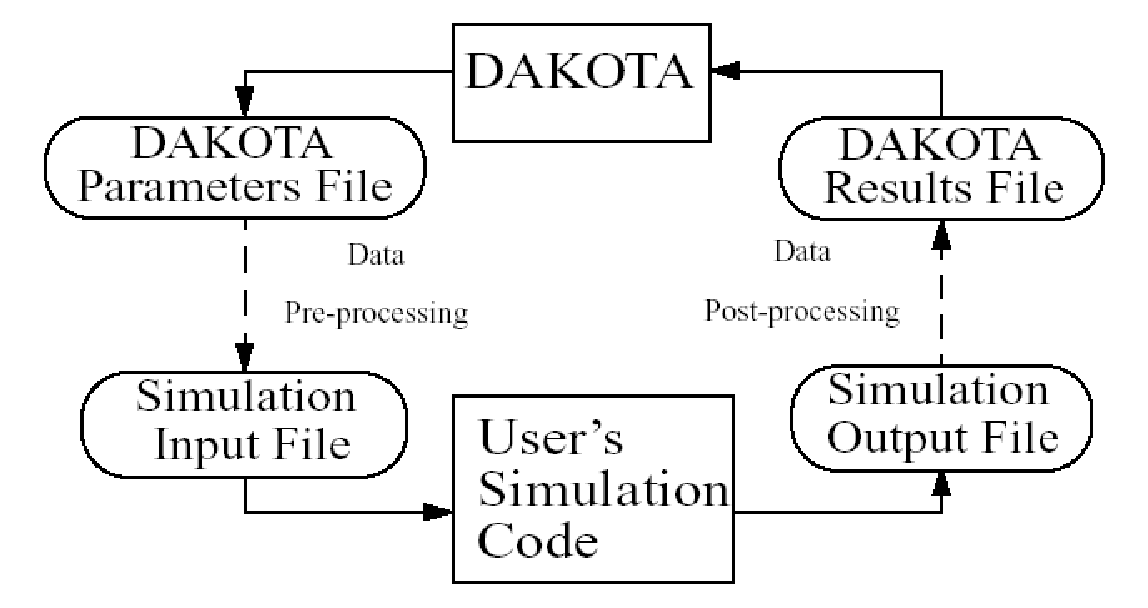
\includegraphics[scale=0.60]{images/dakota_flowchart}
  \caption{The loosely-coupled or ``black-box'' interface between
    Dakota and a user-supplied simulation code.}
  \label{intro:bbinterface}
\end{figure}

The solid lines in Figure~\ref{intro:bbinterface} denote file
input/output (I/O) operations inherent to Dakota or the user's
simulation code. The dotted lines indicate passing or converting
information that must be implemented by the user. As Dakota runs, it
writes out a parameters file containing the current variable values.
Dakota then starts the user's simulation code (or, often, a short
driver script wrapping it), and when the simulation completes, reads
the response data from a results file. This process is repeated until
all of the simulations required by the iterative study are complete.

In some cases it is advantageous to have a close coupling between
Dakota and the simulation code. This close coupling is an advanced
feature of Dakota and is accomplished through either a direct
interface or a SAND (simultaneous analysis and design) interface. For
the direct interface, the user's simulation code is modified to behave
as a function or subroutine under Dakota. This interface can be
considered to be ``semi-intrusive'' in that it requires relatively
minor modifications to the simulation code. Its major advantage is the
elimination of the overhead resulting from file I/O and process
creation. It can also be a useful tool for parallel processing, by
encapsulating all computation in a single executable. For details on
direct interfacing, see Section~\ref{advint:direct}. A SAND interface
approach is ``fully intrusive'' in that it requires further
modifications to the simulation code so that an optimizer has access
to the internal residual vector and Jacobian matrices computed by the
simulation code. In a SAND approach, both the optimization method and
a nonlinear simulation code are converged simultaneously. While this
approach can greatly reduce the computational expense of optimization,
considerable software development effort must be expended to achieve
this intrusive coupling between SAND optimization methods and the
simulation code. SAND may be supported in future Dakota releases.


\section{User's Manual Organization}\label{intro:organization}

The Dakota User's Manual is organized into the following major
categories. New users should consult the Tutorial to get started,
then likely the Method Tour and Interfacing to select a Dakota method
and build an interface to your code. 

\begin{itemize}

\item {\bf Tutorial} (Chapter~\ref{tutorial}): How to obtain, install,
  and use Dakota, with a few introductory examples.

\item {\bf Method Tour} (Chapters~\ref{ps} through~\ref{nls}): Survey
  of the major classes of iterative methods included in Dakota, with
  background, mathematical formulations, usage guidelines, and summary
  of supporting third-party software.

\item {\bf Models} (Chapters~\ref{models} through~\ref{responses}):
  Explanation of Dakota models, which manage the mapping from
  variables through interfaces to responses, as well as details on
  parameter and response file formats for simulation code interfacing.

\item {\bf Input/Output} (Chapters~\ref{input} and~\ref{output}):
  Summary of input to Dakota, including tabular data, and outputs
  generated by Dakota.

\item {\bf Advanced Topics:}
  \begin{itemize}

  \item {\bf Recursion with Components:} Chapter~\ref{adv_meth}
    addresses component-based method recursions, and
    Chapter~\ref{adv_models} addresses component-based model recursions.

  \item {\bf Interfacing:} Chapter~\ref{advint} describes interfacing
    Dakota with engineering simulation codes in both loose- and
    tightly-coupled modes.

  \item {\bf Parallelism:} Chapter~\ref{parallel} describes Dakota's
    parallel computing capabilities, with a summary of major
    application parallel modes in Section~\ref{parallel:application}.

  \item {\bf Fault Tolerance:} Chapter~\ref{restart} describes restart
    capabilities and utilities, and Chapter~\ref{failure} explains ways
    to detect and mitigate simulation failures.

  \end{itemize}

\item {\bf Additional Examples} (Chapter~\ref{additional}):
  Supplemental example analysis problems and discussion.

\end{itemize}

\section{Files Referenced in this Manual}\label{intro:files}
Dakota input files are shown in figures throughout the Manual. 
The filename is specified in the comments
and unless specified otherwise, these
files are available in the {\tt Dakota/examples/users} directory,
where {\tt Dakota} refers to the directory where Dakota was installed. Some
of the input files have associated files, such as output or tabular data,
with the same base filename, and {\tt .sav} appended to the names.

Additional files are referenced, and if the location differs then it will
be specified in the text.
A small number of examples refer to files included only in the source
directory, which is labeled {\tt Dakota\_Source}. You will need a copy of
the source to view these files - see Section~\ref{tutorial:quickstart:installation}.

\section{Summary}\label{intro:summary}

Dakota is both a production tool for engineering design and analysis
activities and a research tool for the development of new algorithms
in optimization, uncertainty quantification, and related areas.
Because of the extensible, object-oriented design of Dakota, it is
relatively easy to add new iterative methods, meta-algorithms,
simulation interfacing approaches, surface fitting methods, etc. In
addition, Dakota can serve as a rapid prototyping tool for algorithm
development. That is, by having a broad range of building blocks
available (i.e., parallel computing, surrogate models, simulation
interfaces, fundamental algorithms, etc.), new capabilities can be
assembled rapidly which leverage the previous software investments.
For additional discussion on framework extensibility, refer to the
Dakota Developers Manual~\cite{DevMan}.

The capabilities of Dakota have been used to solve engineering design
and optimization problems at Sandia Labs, at other Department of
Energy labs, and by our industrial and academic collaborators. Often,
this real-world experience has provided motivation for research into
new areas of optimization. The Dakota development team welcomes
feedback on the capabilities of this software toolkit, as well as
suggestions for new areas of research.

% LocalWords:  UQ nondeterministic epistemic nonlinearity hypercube Behnken
% LocalWords:  multi multifidelity Jacobian

\chapter{Dakota Tutorial}\label{tutorial}

\section {Quickstart}\label{tutorial:installation:quickstart}

This section provides an overview of acquiring and installing Dakota, 
running a simple example, and looking at the basic output available. 
More detailed information about downloads and installation can be found 
on the Dakota website \url{http://dakota.sandia.gov}.

\subsection {Acquiring and Installing Dakota}\label{tutorial:quickstart:installation}

Dakota operates on most systems running Unix or Linux operating
systems as well as on Windows, natively in a Command Prompt window,
and (optionally) with the help of a Cygwin emulation layer. Dakota
is developed and most extensively tested on Redhat Enterprise Linux
with GNU compilers, but additional operating systems
/ compiler combinations are tested nightly as well. See the Dakota
website for more information on supported platforms for particular
Dakota versions.

Department of Energy users: Dakota may already be available on your
target system. Sandia users should visit
\url{http://dakota.sandia.gov/} for information on supported Dakota
installations on engineering networks and cluster computers, as well
as for Sandia-specific downloads. At other DOE institutions, contact
your system administrator about Dakota availability. If Dakota is not
available for your target platform, you may still download Dakota as
described below.

New users should visit \url{https://dakota.sandia.gov/quickstart.html} to
get started with Dakota. This typically involves the following steps:

\begin{enumerate}
  \item Download Dakota. \\
    You may download binary executables for your preferred platforms or 
    you can compile Dakota from source code. Downloads are available from 
    \url{http://dakota.sandia.gov/download.html}.
    
  \item Install Dakota. \\
    Instructions are available from 
    \url{http://dakota.sandia.gov/content/install-dakota}. Guidance is also 
    included in the Dakota source files, including
    \texttt{Dakota\_Source/INSTALL}. Further platform/operating system-specific
    guidance can be found in {\tt Dakota\_Source/examples/platforms}.

  \item Verify that Dakota runs. \\
    To perform a quick check that your Dakota executable runs, open a 
    terminal window (in Windows, cmd.exe), and type: \\
    \vspace{-2em}
    \begin{small}
    \begin{verbatim}
    dakota -v
    \end{verbatim}
      \end{small}
    \vspace{-2em}
    Dakota version information should display in your terminal window.
    For a more detailed description of Dakota command line options, see
    Section~\ref{tutorial:installation:running}.

  \item Participate in Dakota user communities. \\
    Join Dakota mail lists to get the most up-to-date guidance for
    downloading, compiling, installing, or running. For information about
    mail lists, getting help, and other available help resources, see \\
    \url{http://dakota.sandia.gov/content/get-help}.

\end{enumerate}

\subsection{Running Dakota with a simple input file}\label{tutorial:quickstart:running}
This section is intended for users who are new to Dakota, to demonstrate the basics 
of running a simple example. 

{\bf First Steps}
\begin{enumerate}
  \item Make sure Dakota runs. You should see Dakota version information
   when you type: \texttt{dakota -v}
  \item Create a working directory 
  \item Copy \texttt{rosen\_multidim.in} from the \texttt{Dakota/examples/users/}
    directory to the working directory -- see Section~\ref{intro:files} for help.
  \item From the working directory, run \texttt{dakota -i 
    rosen\_multidim.in -o rosen\_multidim.out > rosen\_multidim.stdout}
\end{enumerate}

{\bf What should happen} \\
Dakota outputs a large amount of information to help users track  progress. 
Four files should have been created:
\begin{enumerate}
  \item The screen output has been redirected to the file 
\texttt{rosen\_multidim.stdout}. \\
  The contents are messages from Dakota and notes about the 
progress of the iterator (i.e. method/algorithm).
  \item The output file \texttt{rosen\_multidim.out} 
contains information about the function evaluations.
  \item \texttt{rosen\_multidim.dat} is created due to the 
specification of \texttt{tabular\_graphics\_data} and \\
\texttt{tabular\_graphics\_file}. This summarizes 
the variables and responses for each function evaluation.
  \item \texttt{dakota.rst} is a restart file. If a Dakota 
analysis is interrupted, it can be often be restarted without 
losing all progress.
\end{enumerate}
In addition to the files, some plots are created due to the specification
of \texttt{graphics}. These can be helpful when processing the data or
diagnosing unexpected results.  If your particular installation or build
of Dakota does not support graphics, you will instead get a warning to
this effect.

Dakota has some data processing capabilities for output analysis. 
The output file will contain the relevant results. 
In this case, the output file has details
about each of the 81 function evaluations. 
For more advanced or customized data 
processing or visualization, the tabular data file can be imported into 
another analysis tool. 

{\bf What now?}
\begin{itemize}
  \item Assuming Dakota ran successfully, skim the three text files (restart files are in a binary format). These are described further in 
Section~\ref{tutorial:quickstart:output}.
  \item This example used a parameter study method, and the 
\texttt{rosenbrock} test problem. More details about the example are in
Section~\ref{tutorial:examples:param_study} and the test problem is 
described in Sections~\ref{tutorial:examples:rosenbrock} and~\ref{additional:rosenbrock}.
  \item Explore the many methods available in Dakota in
    Chapters~\ref{ps}--~\ref{nls}.
  \item Try running the other examples in the same directory. These are mentioned
    throughout the manual and are listed in Table~\ref{tutorial:examples:table} 
    for convenience.
  \item Learn the syntax needed to use these methods. For help running Dakota, 
see Section~\ref{tutorial:installation:running} and for input file 
information, see Section~\ref{tutorial:dakota}. 
  \item Learn how to use your own analysis code with Dakota in Chapter~\ref{advint}.
\end{itemize}


\subsection {Examples of Dakota output}\label{tutorial:quickstart:output}
Beyond numerical results, all output files provide information that
allows the user to check that the actual analysis was the intended
analysis. More details on all outputs can be found in Chapter \ref{output}.

{\textbf{Screen output saved to a file}}

Whenever an output file is specified for a Dakota run, the screen
output itself becomes quite minimal consisting of version statements,
environment statements and execution times.

{\textbf{Output file}}

The output file is much more extensive, because it
contains information on every function evaluation (See Figure
\ref{tutorial:quickstart:rosenbrock_multidim:output}). It is 
organized into three basic parts:
\begin{enumerate}
\item Information on the problem
\begin{quote}
For this example, we see that a new restart file is being created
and Dakota has carried out a multidim\_parameter\_study with
8 partitions for each of two variables.
\end{quote}
\item Information on each function evaluation 
\begin{quote}
Each function evaluation is numbered. Details for function evaluation
1 show that at input variable values $x1= -2.0$ and $x2=-2.0$, 
the direct rosenbrock function is being evaluated.  There is one response
with a value of 3.609e+03.
\end{quote}
\item Summary statistics
\begin{quote}
The function evaluation summary is preceded by $<<<<<$. For this
example 81 total evaluations were assessed; all were new, none were
read in from the restart file. Correlation matrices complete the statistics
and output for this problem. Successful runs will finish with
$<<<<<$ Iterator {\it study\_type} completed.
\end{quote}
\end{enumerate}

{\textbf{Tabular output file}}

For this example, the default name for the tabular output file 
\texttt{dakota\_tabular.dat} was changed in the input file to
\texttt{rosen\_multidim.dat}. This tab-delimited text file
(Figure \ref{tutorial:quickstart:rosenbrock_multidim:dat})
summarizes the inputs and outputs to the function evaluator.
The first line contains the names of the variables and responses,
as well as headers for the evaluation id and interface columns.
\begin{verbatim}
   %eval_id   interface   x1   x2   response_fn_1 
\end{verbatim}
The number of function evaluations will match the number of 
evaluations listed in the summary part of the output file for
single method approaches; the names of inputs and outputs will match 
the descriptors specified in the input file. The \texttt{interface} 
column is useful when a Dakota input file contains more than one 
simulation interface. In this instance, there is only one, and
it has no \texttt{id\_interface} specified, so Dakota has supplied
a default value of \texttt{NO\_ID}. This file is ideal for import into
other data analysis packages.


\begin{figure}[ht!]
  \centering
  \begin{bigbox}
    \begin{small}
      \begin{verbatim}
{Writing new restart file dakota.rst
methodName = multidim_parameter_study
gradientType = none
hessianType = none

>>>>> Running multidim_parameter_study iterator.

Multidimensional parameter study for variable partitions of
                                     8
                                     8


------------------------------
Begin Function Evaluation    1
------------------------------
Parameters for function evaluation 1:
                     -2.0000000000e+00 x1
                     -2.0000000000e+00 x2

Direct function: invoking rosenbrock 

Active response data for function evaluation 1:
Active set vector = { 1 }
                      3.6090000000e+03 response_fn_1
.
.
.
<<<<< Function evaluation summary: 81 total (81 new, 0 duplicate)

Simple Correlation Matrix among all inputs and outputs:
                       x1           x2 response_fn_1 
          x1  1.00000e+00 
          x2  1.73472e-17  1.00000e+00 
response_fn_1 -3.00705e-03 -5.01176e-01  1.00000e+00 
. 
.
.
<<<<< Iterator multidim_parameter_study completed.}
\end{verbatim}
    \end{small}
  \end{bigbox}
\caption{Rosenbrock 2-D parameter study example: excerpt from output file}
\label{tutorial:quickstart:rosenbrock_multidim:output}
\end{figure}


\begin{figure}[ht!]
  \centering
  \begin{bigbox}
    \begin{small}
      \begin{verbatim}
%eval_id          interface               x1             x2  response_fn_1 
       1              NO_ID               -2             -2           3609 
       2              NO_ID             -1.5             -2         1812.5 
       3              NO_ID               -1             -2            904 
       4              NO_ID             -0.5             -2          508.5 
\end{verbatim}
    \end{small}
  \end{bigbox}
\label{tutorial:quickstart:rosenbrock_multidim:dat}
\caption{Rosenbrock 2-D parameter study example: excerpt from tabular data file}
\end{figure}


\section{Dakota Input File Format}\label{tutorial:dakota}

See Section~\ref{intro:files} for location of all files referenced in this
manual.

There are six specification blocks that may appear in Dakota input
files. These are identified in the input file using the following
keywords: variables, interface, responses, model, method, and
environment. While, these keyword blocks can appear in any order in a
Dakota input file, there is an inherent relationship that ties them
together. The simplest form of that relationship is shown in
Figure~\ref{tutorial:inputfile_block_layout} and can be summarized as
follows: In each iteration of its algorithm, a \emph{method} block
requests a \emph{variables}-to-\emph{responses} mapping from its
\emph{model}, which the model fulfills through an \emph{interface}.
While most Dakota analyses satisfy this relationship, where a single
method runs a single model, advanced cases are possible and are
discussed in Chapter~\ref{adv_meth}.

\begin{figure}[ht!]
  \centering
  \includegraphics[height=2.5in]{images/InputBlocks}
  \caption{Relationship between the six blocks, for a simple study.}
  \label{tutorial:inputfile_block_layout}
\end{figure}

As a concrete example, a simple Dakota input file,
\texttt{rosen\_multidim.in}, is shown in
Figure~\ref{tutorial:rosenbrock_multidim} for a two-dimensional
parameter study on Rosenbrock's function.  This input file will be
used to describe the basic format and syntax used in all Dakota input
files.  The results are shown later, in
Section~\ref{tutorial:examples:param_study}.

\begin{figure}[ht!]
  \centering
  \begin{bigbox}
    \begin{small}
      \verbatimtabinput[8]{rosen_multidim.in}
    \end{small}
  \end{bigbox}
  \caption{Rosenbrock 2-D parameter study example: the Dakota input
    file.}
  \label{tutorial:rosenbrock_multidim}
\end{figure}

The first block of the input file shown in
Figure~\ref{tutorial:rosenbrock_multidim} is the \emph{environment}
block.  This keyword block is used to specify the general Dakota
settings such as Dakota's graphical output (via the \texttt{graphics}
flag) and the tabular data output (via the
\texttt{tabular\_graphics\_data} keyword).  In advanced cases, it also
identifies the \texttt{top\_method\_pointer} that will control the
Dakota study.  The \emph{environment} block is optional, and at most
one such block can appear in a Dakota input file.

The \emph{method} block of the input file specifies which iterative
method Dakota will employ and associated method options.
The keyword \texttt{multidim\_parameter\_study} in
Figure~\ref{tutorial:rosenbrock_multidim} calls for a multidimensional
parameter study, while the keyword \texttt{partitions} specifies the
number of intervals per variable (a method option). In this case,
there will be eight intervals (nine data points) evaluated between the
lower and upper bounds of both variables (bounds provided subsequently
in the \emph{variables} section), for a total of 81 response function
evaluations.  At least one \emph{method} block is required, and
multiple blocks may appear in Dakota input files for advanced studies.

The \emph{model} block of the input file specifies the model that
Dakota will use. A model provides the logical unit for determining how
a set of variables is mapped through an interface into a set of
responses when needed by an iterative method. In the default case, the
model allows one to specify a single set of variables, interface, and
responses.  The \emph{model} block is optional in this simple case.
Alternatively, it can be explicitly defined as in
Figure~\ref{tutorial:rosenbrock_multidim}, where the keyword
\texttt{single} specifies the use of a single model in the parameter
study.  If one wishes to perform more sophisticated studies such as
surrogate-based analysis or optimization under uncertainty, the
logical organization specified in the \emph{model} block becomes
critical in informing Dakota on how to manage the different components
of such studies, and multiple \emph{model} blocks are likely needed.
See Chapter~\ref{models} for relevant advanced model specification
details.

The \emph{variables} block of the input file specifies the number,
type, and characteristics of the parameters that will be varied by
Dakota. The variables can be classified as design variables, uncertain
variables, or state variables.  Design variables are typically used in
optimization and calibration, uncertain variables are used in UQ and
sensitivity studies, and state variables are usually fixed.  In all
three cases, variables can be continuous or discrete, with discrete
having real, integer, and string subtypes. See Chapter~\ref{variables}
for more information on the types of variables supported by
Dakota. The \emph{variables} section shown in
Figure~\ref{tutorial:rosenbrock_multidim} specifies that there are two
continuous design variables. The sub-specifications for continuous
design variables provide the descriptors ``x1'' and ``x2'' as well as
lower and upper bounds for these variables. The information about the
variables is organized in column format for readability. So, both
variables $x_1$ and $x_2$ have a lower bound of -2.0 and an upper
bound of 2.0. At least one \emph{variables} block is required, and
multiple blocks may appear in Dakota input files for advanced studies.

The \emph{interface} block of the input file specifies the simulation
code that will be used to map variables into responses as well as
details on how Dakota will pass data to and from that code.  In this
example, the keyword \texttt{direct} is used to indicate the use of a
function linked directly into Dakota, and data is passed directly
between the two.  The name of the function is identified by the
\texttt{analysis\_driver} keyword.  Alternatively, \texttt{fork} or
\texttt{system} executions can be used to invoke instances of a
simulation code that is external to Dakota as explained in Section
\ref{tutorial:examples:user_supply:optimization2} and
Chapter~\ref{advint}.  In this case, data is passed between Dakota and
the simulation via text files. At least one \emph{interface} block is
required, and multiple blocks may appear in Dakota input files for
advanced studies.

The \emph{responses} block of the input file specifies the types of
data that the interface will return to Dakota.  They are categorized
primarily according to usage.  Objective functions are used in
optimization, calibration terms in calibration, and response functions
in sensitivity analysis and UQ. For the example shown in
Figure~\ref{tutorial:rosenbrock_multidim}, the assignment
\texttt{response\_functions = 1} indicates that there is only one
response function. The \emph{responses} block can include additional
information returned by the interface.  That includes constraints and
derivative information, both discussed in Chapter~\ref{responses}.  In
this example, there are no constraints associated with Rosenbrock's
function, so the keywords for constraint specifications are
omitted. The keywords \texttt{no\_gradients} and \texttt{no\_hessians}
indicate that no derivatives will be provided to the method; none are
needed for a parameter study.  At least one \emph{responses} block is
required, and multiple blocks may appear in Dakota input files for
advanced studies.

We close this section with a list of rules regarding the formatting of
the Dakota input file.
\begin{itemize}
\item ``Flat'' text only.
\item Whitespace is ignored.
\item Comments begin with \# and continue to the end of the line.
\item Keyword order is largely unimportant as long as major sections
  are respected and there is no ambiguity.
\item Equal signs are optional.
\item Strings can be surrounded by single or double quotes (but not
  ``fancy'' quotes).
\item Scientific notation is fine.
\end{itemize}
Please see the Dakota Reference Manual~\cite{RefMan} for additional
details on this input file syntax.

\section{Examples}\label{tutorial:examples}

This section serves to familiarize users with how to perform parameter 
studies, optimization, and uncertainty quantification through their common
Dakota interface. The initial examples utilize simple built in driver 
functions; later we show how to utilize Dakota to drive the evaluation of 
user supplied black box code. The examples presented in this chapter 
are intended to show the simplest use of Dakota for methods of 
each type. More advanced examples of using Dakota for specific purposes 
are provided in subsequent, topic-based, chapters.

\subsection{Rosenbrock Test Problem}\label{tutorial:examples:rosenbrock}

The examples shown later in this chapter use the Rosenbrock
function \cite{Rosenbrock60} (also described in \cite{Gil81}, among
other places), which has the form:

\begin{equation}
f(x_1,x_2)=100(x_2-x_1^2)^2+(1-x_1)^2 \label{tutorial:rosen}
\end{equation}

A three-dimensional plot of this function is shown in
Figure~\ref{tutorial:rosenbrock_prob}(a), where both $x_1$ and
$x_2$ range in value from $-2$ to $2$.
Figure~\ref{tutorial:rosenbrock_prob}(b) shows a contour plot
for Rosenbrock's function. An optimization problem using Rosenbrock's
function is formulated as follows:

\begin{eqnarray}
\texttt{minimize }   & & f(x_1,x_2)          \nonumber\\
                     & & \mathbf{x} \in \Re^2\nonumber\\
\texttt{subject to } & & -2 \le x_1 \le 2    \\
                     & & -2 \le x_2 \le 2    \nonumber
\end{eqnarray}

\begin{figure}[htp!]
  \centering
  \begin{tabular}{cc}
  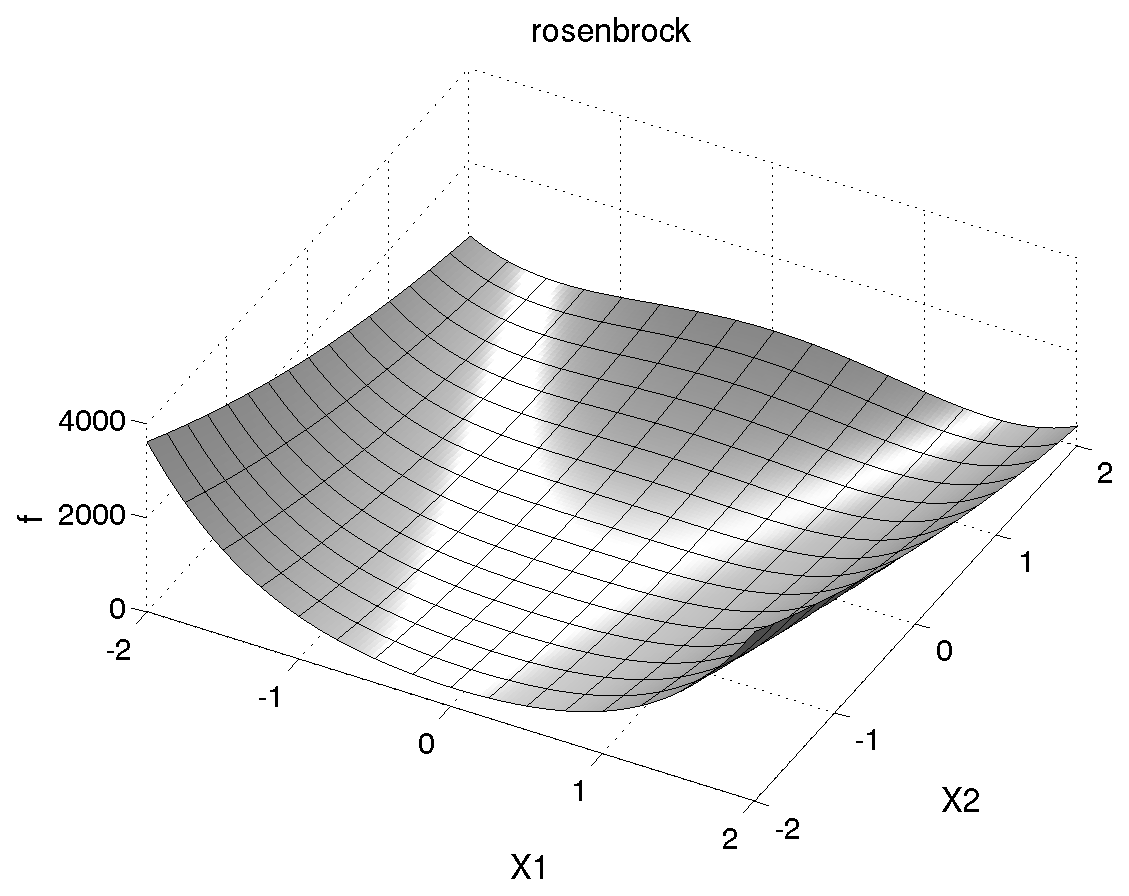
\includegraphics[height=2.5in]{images/rosen_3d_surf} &
  \includegraphics[height=2.5in]{images/rosen_2d_surf} \\
  (a) & (b) \\
  \end{tabular}
  \caption{Rosenbrock's function: (a) 3-D plot and (b) contours with
  $x_1$ on the bottom axis.}
  \label{tutorial:rosenbrock_prob}
\end{figure}

Note that there are no linear or nonlinear constraints in this
formulation, so this is a bound constrained optimization problem. The
unique solution to this problem lies at the point
$(x_1,x_2) = (1,1)$, where the function value is zero.

Several other test problems are available. See
Chapter~\ref{additional} for a description of these test problems
as well as further discussion of the Rosenbrock test problem.


\subsection{Two-Dimensional Grid Parameter Study}\label{tutorial:examples:param_study}

Parameter study methods in the Dakota toolkit involve the computation 
of response data sets at a selection of points in the parameter space. 
These response data sets are not linked to any specific interpretation,
so they may consist of any allowable specification from the responses 
keyword block, i.e., objective and constraint functions, least squares 
terms and constraints, or generic response functions. This allows the 
use of parameter studies in direct coordination with optimization, least 
squares, and uncertainty quantification studies without significant
modification to the input file. 

An example of a parameter study is the 2-D parameter study example problem 
listed in Figure~\ref{tutorial:rosenbrock_multidim}. This is 
executed by Dakota using the command noted in the comments:
\begin{small}
\begin{verbatim}
    dakota -i rosen_multidim.in -o rosen_multidim.out > rosen_multidim.stdout
\end{verbatim}
\end{small}

The output of the Dakota run is written to the file named
\texttt{rosen\_multidim.out} while the screen output, or
standard output, is redirect to \texttt{rosen\_multidim.stdout}.
For comparison, files named \texttt{rosen\_multidim.out.sav}
and \texttt{rosen\_multidim.stdout.sav} are included in the
\texttt{Dakota/examples/users} directory. As for many of the examples,
Dakota provides a report on the best design point located during the
study at the end of these output files.

This 2-D parameter study produces the grid of data samples shown in
Figure~\ref{tutorial:rosenbrock_multidim_graphics}. In general, a multidimensional 
parameter study lets one generate a grid in multiple dimensions. 
The keyword \texttt{multidim\_parameter\_study} indicates that 
a grid will be generated over all variables. The keyword 
\texttt{partitions} indicates the number of grid partitions in 
each dimension. For this example, the number of the grid partitions 
are the same in each dimension (8 partitions) but it would be possible 
to specify (partitions = 8 2), and have only two partitions 
over the second input variable.  Note that the
\texttt{graphics} flag in the \emph{environment} block of the input
file could be commented out since, for this example, the iteration
history plots created by Dakota are not particularly instructive. More
interesting visualizations can be created by importing Dakota's
tabular data into an external graphics/plotting package. Common
graphics and plotting packages include Mathematica, Matlab, Microsoft
Excel, Origin, Tecplot, Gnuplot and many others. (Sandia National Laboratories
and the Dakota developers do not endorse any of these commercial
products.)

\begin{figure}[htb!]
  \centering
  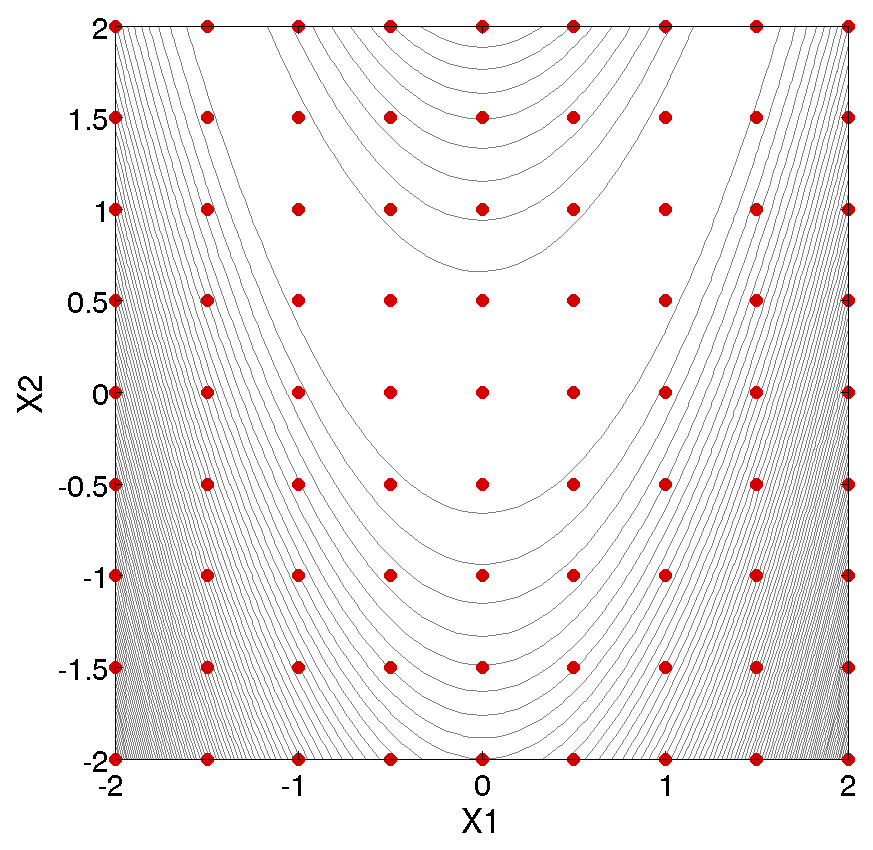
\includegraphics[height=2.5in]{images/rosen_2d_pts}
  \caption{Rosenbrock 2-D parameter study example:
  location of the design points (dots) evaluated.}
  \label{tutorial:rosenbrock_multidim_graphics}
\end{figure}


\subsection{Gradient-based Unconstrained Optimization}\label{tutorial:examples:optimization}

Dakota's optimization capabilities include a variety of gradient-based 
and nongradient-based optimization methods. This subsection demonstrates
the use of one such method through the Dakota interface.

A Dakota input file for a gradient-based optimization of Rosenbrock's
function is listed in Figure~\ref{tutorial:rosenbrock_grad}. The
format of the input file is similar to that used for the parameter
studies, but there are some new keywords in the responses and method
sections. First, in the responses block of the input file, the
keyword block starting with \texttt{numerical\_gradients} specifies
that a finite difference method will be used to compute gradients for
the optimization algorithm. Note that the Rosenbrock function
evaluation code inside Dakota has the ability to give analytical
gradient values. (To switch from finite difference gradient estimates
to analytic gradients, uncomment the \texttt{analytic\_gradients}
keyword and comment out the four lines associated with the
\texttt{numerical\_gradients} specification.)
Next, in the method
block of the input file, several new keywords have been added. In
this block, the keyword \texttt{conmin\_frcg} indicates the use of
the Fletcher-Reeves conjugate gradient algorithm in the CONMIN
optimization software package~\cite{Van78} for bound-constrained
optimization. The keyword \texttt{max\_iterations} is used to
indicate the computational budget for this optimization (in this case,
a single iteration includes multiple evaluations of Rosenbrock's
function for the gradient computation steps and the line search
steps). The keyword \texttt{convergence\_tolerance} is used to specify
one of CONMIN's convergence criteria (under which CONMIN terminates if the
objective function value differs by less than the absolute value of
the convergence tolerance for three successive iterations).
% And, finally, the \texttt{output} verbosity is set to \texttt{quiet}.

\begin{figure}
  \centering
  \begin{bigbox}
    \begin{small}
      \verbatimtabinput[8]{rosen_grad_opt.in}
    \end{small}
  \end{bigbox}
  \caption{Rosenbrock gradient-based unconstrained optimization
  example: the Dakota input file.}
  \label{tutorial:rosenbrock_grad}
\end{figure}

The Dakota command is noted in the file, and copies of the outputs
are in the \texttt{Dakota/examples/users} directory, with \texttt{.sav}
appended to the name.  When this example problem is executed using
Dakota with graphics support enabled, Dakota creates some iteration
history graphics similar to the screen capture shown in Figure~
\ref{tutorial:rosenbrock_grad_graphics}(a). These plots show how the
objective function and design parameters change in value during the
optimization steps. The scaling of the horizontal and vertical axes
can be changed by moving the scroll knobs on each plot.  Also, the
``Options'' button allows the user to plot the vertical axes using a
logarithmic scale. Note that log-scaling is only allowed if the values
on the vertical axis are strictly greater than zero.

\begin{figure}[ht!]
  \centering
  \begin{tabular}{c}
  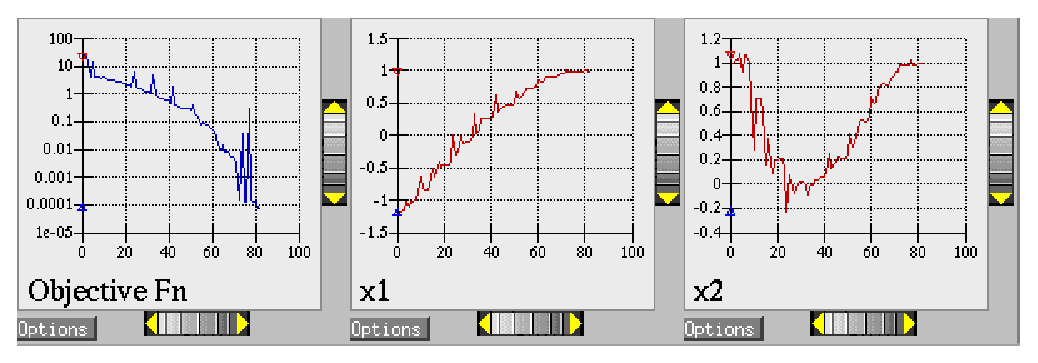
\includegraphics[width=\textwidth]{images/dak_graphics_grad_opt}\\
  (a)\\
  \qquad\\
  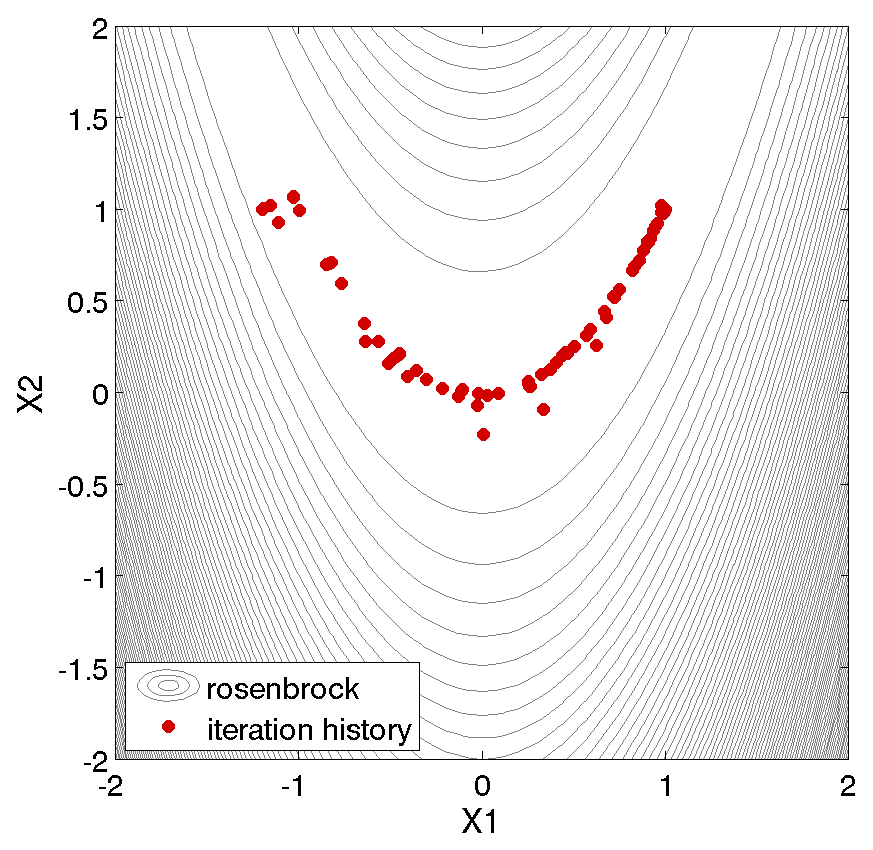
\includegraphics[height=2.5in]{images/rosen_grad_opt_pts} \\
  (b)
  \end{tabular}
  \caption{Rosenbrock gradient-based unconstrained optimization
    example: (a) screen capture of the Dakota graphics and (b)
    sequence of design points (dots) evaluated (line search points
    omitted).}
  \label{tutorial:rosenbrock_grad_graphics}
\end{figure}

Figure~\ref{tutorial:rosenbrock_grad_graphics}(b) shows the
iteration history of the optimization algorithm. The optimization
starts at the point $(x_1,x_2) = (-1.2,1.0)$ as given in the
Dakota input file. Subsequent iterations follow the banana-shaped
valley that curves around toward the minimum point at $(x_1,x_2) =
(1.0,1.0)$. Note that the function evaluations associated with the
line search phase of each CONMIN iteration are not shown on the plot.
At the end of the Dakota run, information is written to the output
file to provide data on the optimal design point. These data include
the optimum design point parameter values, the optimum objective and
constraint function values (if any), plus the number of function
evaluations that occurred and the amount of time that elapsed during
the optimization study.

\subsection{Uncertainty Quantification with Monte Carlo Sampling}\label{tutorial:examples:uncert_quant}

Uncertainty quantification (UQ) is the process of determining the
effect of input uncertainties on response metrics of interest. These
input uncertainties may be characterized as either aleatory
uncertainties, which are irreducible variabilities inherent in nature,
or epistemic uncertainties, which are reducible uncertainties
resulting from a lack of knowledge. Since sufficient data is
generally available for aleatory uncertainties, probabilistic methods
are commonly used for computing response distribution statistics based
on input probability distribution specifications. Conversely, for
epistemic uncertainties, data is generally sparse, making the use of
probability theory questionable and leading to nonprobabilistic
methods based on interval specifications.

The subsection demonstrates the use of Monte Carlo random sampling
for Uncertainty Quantification.

Figure~\ref{tutorial:rosenbrock_mc} shows the Dakota input file for
an example problem that demonstrates some of the random sampling
capabilities available in Dakota. In this example, the design
parameters, x1 and x2, will be treated as uncertain parameters that
have uniform distributions over the interval [-2, 2]. This is
specified in the variables block of the input file, beginning with
the keyword \texttt{uniform\_uncertain}.
% Not true: For comparison, the keywords
% from the previous examples are retained, but have been commented out.
Another difference from earlier input files such as
Figure~\ref{tutorial:rosenbrock_grad}
occurs in the responses block, where
the keyword \texttt{response\_functions} is used in place of
\texttt{objective\_functions}. The final changes to the input
file occur in the method block, where the keyword
\texttt{sampling} is used.

The other keywords in the methods block of the input file
specify the number of samples (200), the seed for the random number
generator (17), the sampling method (random), and the response
threshold (100.0). The \texttt{seed} specification allows a user to
obtain repeatable results from multiple runs. If a seed value is not
specified, then Dakota's sampling methods are designed to generate
nonrepeatable behavior (by initializing the seed using a system
clock). The keyword \texttt{response\_levels} allows the user to
specify threshold values for which Dakota will compute statistics on
the response function output. Note that a unique threshold value can
be specified for each response function.

In this example, Dakota will select 200 design points from within the
parameter space, evaluate the value of Rosenbrock's function at all
200 points, and then perform some basic statistical calculations on
the 200 response values.

The Dakota command is noted in the file, and copies of the outputs
are in the \texttt{Dakota/examples/users} directory, with \texttt{.sav} 
appended to the name.  
Figure~\ref{tutorial:results_mc} shows example results from this 
sampling method. 
Note that your results will differ from those in
this file if your \texttt{seed} value differs or if no \texttt{seed}
is specified.

As shown in Figure~\ref{tutorial:results_mc}, 
the statistical data on the 200 Monte Carlo samples is printed at the
end of the output file in the section that starts with ``Statistics
based on 200 samples.'' In this section summarizing 
moment-based statistics, Dakota outputs the
mean, standard deviation, skewness, and kurtosis estimates 
for each of the response functions. For example, 
the mean of the Rosenbrock function given uniform input uncertainties 
on the input variables is 455.4 and the standard deviation is 536.8. 
This is a very large standard deviation, due to the fact that the 
Rosenbrock function varies by three orders of magnitude over the input 
domain. The skewness is positive, meaning this is a right-tailed distribution, 
not a symmetric distribution. Finally, the kurtosis (a measure of the 
``peakedness'' of the distribution) indicates that 
this is a strongly peaked distribution (note that we use a central, 
standardized kurtosis so that the kurtosis of a normal is zero). 
After the moment-related statistics, the 95\% confidence intervals on the 
mean and standard deviations are printed. This is followed by
the fractions (``Probability Level'') of the response function values 
that are below the response threshold values specified in the input file. 
For example, 34 percent of the sample inputs resulted in a Rosenbrock 
function value that was less than or equal to 100, as shown in the line 
listing the cumulative distribution function values. 
Finally, there are several 
correlation matrices printed at the end, showing simple and partial 
raw and rank correlation matrices. Correlations provide an indication 
of the strength of a monotonic relationship between input and outputs. 
More detail on correlation coefficients and their interpretation can be 
found in Section~\ref{uq:uncertainty1}. 
More detail about sampling methods in general can be found in 
Section~\ref{uq:sampling}. Finally,  
Figure~\ref{tutorial:rosenbrock_mc_points} shows the locations
of the 200 sample sites within the parameter space of the Rosenbrock
function for this example.

\begin{figure}[ht!]
  \centering
  \begin{bigbox}
    \begin{small}
      \verbatimtabinput[8]{rosen_sampling.in}
    \end{small}
  \end{bigbox}
  \caption{Monte Carlo sampling example: the Dakota input file.}
  \label{tutorial:rosenbrock_mc}
\end{figure}

\begin{figure}
\centering
\begin{bigbox}
\begin{footnotesize}
\begin{verbatim}
Statistics based on 200 samples:

Moment-based statistics for each response function:
                            Mean           Std Dev          Skewness          Kurtosis
 response_fn_1  4.5540183516e+02  5.3682678089e+02  1.6661798252e+00  2.7925726822e+00

95% confidence intervals for each response function:
                    LowerCI_Mean      UpperCI_Mean    LowerCI_StdDev    UpperCI_StdDev
 response_fn_1  3.8054757609e+02  5.3025609422e+02  4.8886795789e+02  5.9530059589e+02

Level mappings for each response function:
Cumulative Distribution Function (CDF) for response_fn_1:
     Response Level  Probability Level  Reliability Index  General Rel Index
     --------------  -----------------  -----------------  -----------------
   1.0000000000e+02   3.4000000000e-01

Probability Density Function (PDF) histograms for each response function:
PDF for response_fn_1:
          Bin Lower          Bin Upper      Density Value
          ---------          ---------      -------------
   1.1623549854e-01   1.0000000000e+02   3.4039566059e-03
   1.0000000000e+02   2.7101710856e+03   2.5285698843e-04

Simple Correlation Matrix among all inputs and outputs:
                       x1           x2 response_fn_1 
          x1  1.00000e+00 
          x2 -5.85097e-03  1.00000e+00 
response_fn_1 -9.57746e-02 -5.08193e-01  1.00000e+00 

Partial Correlation Matrix between input and output:
             response_fn_1 
          x1 -1.14659e-01 
          x2 -5.11111e-01 

Simple Rank Correlation Matrix among all inputs and outputs:
                       x1           x2 response_fn_1 
          x1  1.00000e+00 
          x2 -6.03315e-03  1.00000e+00 
response_fn_1 -1.15360e-01 -5.04661e-01  1.00000e+00 

Partial Rank Correlation Matrix between input and output:
             response_fn_1 
          x1 -1.37154e-01 
          x2 -5.08762e-01 
\end{verbatim}
\end{footnotesize}
\end{bigbox}
\caption{Results of Monte Carlo Sampling on the Rosenbrock Function}
\label{tutorial:results_mc}
\end{figure}


\begin{figure}[ht!]
  \centering
  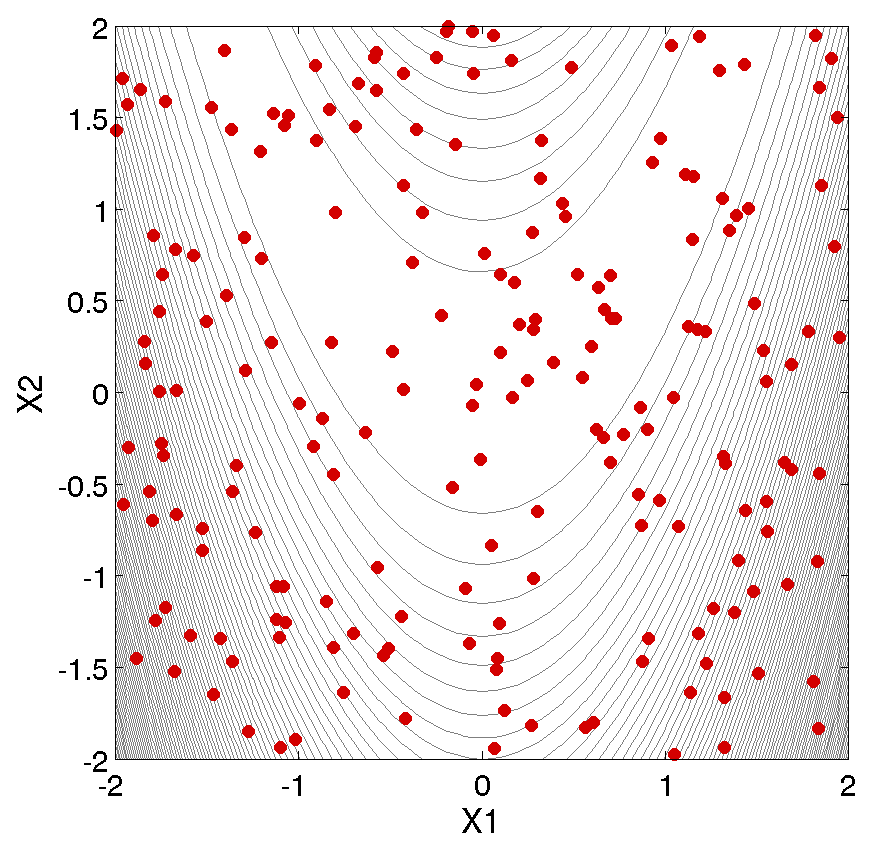
\includegraphics[height=2.5in]{images/rosen_nond_pts}
  \caption{Monte Carlo sampling example: locations in the parameter
    space of the 200 Monte Carlo samples using a uniform distribution
    for both $x_1$ and $x_2$.}
  \label{tutorial:rosenbrock_mc_points}
\end{figure}

\subsection{User Supplied Simulation Code Examples}\label{tutorial:examples:user_supply}
This subsection provides examples of how to use Dakota to drive user 
supplied black box code.

\subsubsection{Optimization with a User-Supplied Simulation Code - Case 1}\label{tutorial:examples:user_supply:optimization1}

Many of the previous examples made use of the direct interface to
access the Rosenbrock and textbook test functions that are compiled
into Dakota. In engineering applications, it is much more common to
use the \texttt{fork} interface approach within
Dakota to manage external simulation codes. In both of these cases,
the communication between Dakota and the external code is conducted
through the reading and writing of short text files. For this example,
the C++ program \texttt{rosenbrock.cpp} in \texttt{Dakota\_Source/test} is used
as the simulation code. This file is compiled to create the
stand-alone \texttt{rosenbrock} executable that is referenced as the
\texttt{analysis\_driver} in Figure~\ref{tutorial:rosenbrock_user}.
This stand-alone program performs the same function evaluations as
Dakota's internal Rosenbrock test function.

Figure~\ref{tutorial:rosenbrock_user} shows the text of the Dakota
input file named \texttt{rosen\_syscall.in} that is
provided in the directory \texttt{Dakota/examples/users}.
The only differences between this input file and the one in Figure~
\ref{tutorial:rosenbrock_grad} occur in the \emph{interface} keyword
section. The keyword \texttt{fork} indicates that Dakota will use
fork calls to create separate Unix processes for executions of the
user-supplied simulation code. The name of the simulation code, and
the names for Dakota's parameters and results file are specified using
the \texttt{analysis\_driver}, \texttt{parameters\_file}, and
\texttt{results\_file} keywords, respectively.

The Dakota command is noted in the file, and copies of the outputs
are in the \texttt{Dakota/examples/users} directory, with \texttt{.sav} 
appended to the name.  

This run of Dakota takes longer to complete than the previous
gradient-based optimization example since the \texttt{fork}
interface method has additional process creation and file I/O
overhead, as compared to the internal communication that occurs when
the \texttt{direct} interface method is used. 

To gain a better understanding of what exactly Dakota is doing with
the \texttt{fork} interface approach, add the keywords
\texttt{file\_tag} and \texttt{file\_save} to the interface
specification and re-run Dakota. Check the listing of the local
directory and you will see many new files with names such as
\texttt{params.in.1}, \texttt{params.in.2}, etc., and
\texttt{results.out.1}, \texttt{results.out.2}, etc. There is one
\texttt{params.in.X} file and one \texttt{results.out.X} file for each
of the function evaluations performed by Dakota. This is the file
listing for \texttt{params.in.1}:
%\newpage
\begin{small}
\begin{verbatim}
                                          2 variables
                     -1.200000000000000e+00 x1
                      1.000000000000000e+00 x2
                                          1 functions
                                          1 ASV_1:obj_fn
                                          2 derivative_variables
                                          1 DVV_1:x1
                                          2 DVV_2:x2
                                          0 analysis_components
\end{verbatim}
\end{small}

\begin{figure}[b!]
  \begin{bigbox}
    \begin{small}
      \verbatimtabinput[8]{rosen_syscall.in}
    \end{small}
  \end{bigbox}
  \caption{Dakota input file for gradient-based optimization using the
    fork call interface to an external rosenbrock simulator.}
  \label{tutorial:rosenbrock_user}
\end{figure}

The basic pattern is that of array lengths and string identifiers
followed by listings of the array entries, where the arrays consist of
the variables, the active set vector (ASV), the derivative values
vector (DVV), and the analysis components (AC). For the variables
array, the first line gives the total number of variables (2) and the
``variables'' string identifier, and the subsequent two lines provide
the array listing for the two variable values (-1.2 and 1.0) and
descriptor tags (``x1'' and ``x2'' from the Dakota input file). The
next array conveys the ASV, which indicates what
simulator outputs are needed. The first line of the array gives the total number
of response functions (1) and the ``functions'' string identifier,
followed by one ASV code and descriptor tag
(``ASV\_1'') for each function. In this case, the ASV value of 1 indicates that Dakota
is requesting that the simulation code return the response function
value in the file \texttt{results.out.X}. (Possible ASV values: 1 = value of
response function value, 2 = response function gradient, 4 = response
function Hessian, and any sum of these for combinations up to
7 = response function value, gradient, and Hessian; see ~\ref{variables:asv} for
more detail.)  The next array provides the DVV, which defines the
variable identifiers used in computing derivatives. The first line of
the array gives the number of derivative variables (2) and the
``derivative\_variables'' string identifier, followed by the listing of
the two DVV variable identifiers (the first and second variables) and
descriptor tags (``DVV\_1'' and ``DVV\_2''). The final array provides
the AC array used to provide additional strings for use by the
simulator (e.g., to provide the name of a particular mesh file). The
first line of the array gives the total number of analysis components
(0) and the ``analysis\_components'' string identifier, followed by the
listing of the array, which is empty in this case.

The executable program rosenbrock reads in the \texttt{params.in.X}
file and evaluates the objective function at the given values for
$x_1$ and $x_2$. Then, rosenbrock writes out
the objective function data to the \texttt{results.out.X} file. Here
is the listing for the file \texttt{results.out.1}:
\begin{small}
\begin{verbatim}
                     2.420000000000000e+01 f
\end{verbatim}
\end{small}

The value shown above is the value of the objective function, and the
descriptor `f' is an optional tag returned by the simulation code.
When the fork call has completed, Dakota reads in the data from the
\texttt{results.in.X} file and processes the results. Dakota then
continues with additional executions of the rosenbrock program until
the optimization process is complete.

\subsubsection{Optimization with a User-Supplied Simulation Code - Case 2}\label{tutorial:examples:user_supply:optimization2}

In many situations the user-supplied simulation code cannot be
modified to read and write the \texttt{params.in.X file} and the
\texttt{results.out.X} file, as described above. Typically, this
occurs when the simulation code is a commercial or proprietary
software product that has specific input file and output file formats.
In such cases, it is common to replace the executable program name in
the Dakota input file with the name of a Unix shell script containing
a sequence of commands that read and write the necessary files and run
the simulation code. For example, the executable program named
\texttt{rosenbrock} listed in Figure~\ref{tutorial:rosenbrock_user}
could be replaced by a Unix Bourne or C-shell script named
\texttt{simulator\_script}, with the script containing a sequence of
commands to perform the following steps: insert the data from the
\texttt{parameters.in.X} file into the input file of the simulation
code, execute the simulation code, post-process the files generated by
the simulation code to compute response data, and return the response
data to Dakota in the \texttt{results.out.X} file. The steps that are
typically used in constructing and using a Unix shell script are
described in Section~\ref{interfaces:building}.

\section{Dakota Command-Line Options}\label{tutorial:installation:running}

The Dakota executable file is named {\tt dakota} ({\tt dakota.exe} on
Windows). If this command is entered at the command prompt without any
arguments, a usage message similar to the following appears:
\begin{small}
\begin{verbatim}
usage: dakota [options and <args>]
        -help (Print this summary)
        -version (Print Dakota version number)
        -input <$val> (REQUIRED Dakota input file $val)
        -output <$val> (Redirect Dakota standard output to file $val)
        -error <$val> (Redirect Dakota standard error to file $val)
        -parser <$val> (Parsing technology: nidr[strict][:dumpfile])
        -no_input_echo (Do not echo Dakota input file)
        -check (Perform input checks)
        -pre_run [$val] (Perform pre-run (variables generation) phase)
        -run [$val] (Perform run (model evaluation) phase)
        -post_run [$val] (Perform post-run (final results) phase)
        -read_restart [$val] (Read an existing Dakota restart file $val)
        -stop_restart <$val> (Stop restart file processing at evaluation $val)
        -write_restart [$val] (Write a new Dakota restart file $val)
\end{verbatim}
\end{small}
%$ this comment is here to trick xemacs into highlighting syntax correctly

Of these available command line inputs, only the ``\texttt{-input}''
option is required, and ``\texttt{-input}'' can be omitted if the
input file name is the final item on the command line; all other
command-line inputs are optional. The ``\texttt{-help}'' option prints
the usage message above. The ``\texttt{-version}'' option prints the
version number of the executable. The ``\texttt{-check}'' option
invokes a dry-run mode in which the input file is processed and
checked for errors, but the study is not performed. The
``\texttt{-input}'' option provides the name of the Dakota input file.
The ``\texttt{-output}'' and ``\texttt{-error}'' options provide file
names for redirection of the Dakota standard output (stdout) and
standard error (stderr), respectively. By default, Dakota will echo
the input file to the output stream, but ``\texttt{-no\_input\_echo}''
can override this behavior.

The ``\texttt{-parser}'' input is for debugging and will not
be further described here. The ``\texttt{-read\_restart}''
and ``\texttt{-write\_restart}'' options provide the names of
restart databases to read from and write to, respectively. The
``\texttt{-stop\_restart}'' option limits the number of
function evaluations read from the restart database (the default is all
the evaluations) for those cases in which some evaluations were erroneous
or corrupted. Restart management is an important technique for retaining
data from expensive engineering applications. This advanced topic is
discussed in detail in Chapter~\ref{restart}. Note that these command
line options can be abbreviated so long as the abbreviation is unique.
Accordingly, the following are valid, unambiguous specifications: ``\texttt{-h}'',
``\texttt{-v}'', ``\texttt{-c}'', ``\texttt{-i}'', ``\texttt{-o}'',
``\texttt{-e}'', ``\texttt{-re}'', ``\texttt{-s}'', ``\texttt{-w}'',
``\texttt{-pr}'', ``\texttt{-ru}'', and ``\texttt{-po}'' and can be used
in place of the longer forms of the command line options.

To run Dakota with a particular input file, the following syntax can
be used:
\begin{small}
\begin{verbatim}
    dakota -i dakota.in
\end{verbatim}
\end{small}
or more simply
\begin{small}
\begin{verbatim}
    dakota dakota.in
\end{verbatim}
\end{small}

This will echo the standard output (stdout) and standard error
(stderr) messages to the terminal. To redirect stdout and stderr to
separate files, the \texttt{-o} and \texttt{-e} command line options
may be used:
\begin{small}
\begin{verbatim}
    dakota -i dakota.in -o dakota.out -e dakota.err
\end{verbatim}
\end{small}
or
\begin{small}
\begin{verbatim}
    dakota -o dakota.out -e dakota.err dakota.in
\end{verbatim}
\end{small}

Alternatively, any of a variety of Unix redirection variants can be
used. The simplest of these redirects stdout to another file:
\begin{small}
\begin{verbatim}
    dakota dakota.in > dakota.out
\end{verbatim}
\end{small}

% this is not a linux tutorial.
% To append to a file rather than overwrite it, ``\texttt{>>}'' is used
% in place of ``\texttt{>}''. The syntax to redirect stderr as well as stdout
% to the same file depends on the shell you are using. With csh, simply append
% ``\texttt{\&}'' with no embedded space, i.e.,
% ``\texttt{>\&}'' or ``\texttt{>>\&}''. With the Bourne shell (sh or bash) use
% ``\texttt{>dakota.out 2>\&1}'' or ``\texttt{>>dakota.out 2>\&1}''.
% With csh, if you have the noclobber environment variable set but
% wish either to overwrite an existing output file or to append to a file that
% does not yet exist, append ``\texttt{!}'' to the redirection operators
% (with no intervening spaces), i.e.,
% ``\texttt{>!}'', ``\texttt{>\&!}'', ``\texttt{>>!}'', or
% ``\texttt{>>\&!}''.

To run the dakota process in the background, append an ampersand
symbol (\&) to the command with an embedded space, e.g.,
\begin{small}
\begin{verbatim}
    dakota dakota.in > dakota.out &
\end{verbatim}
\end{small}

Refer to~\cite{And86} for more information on Unix redirection and
background commands.

The ``\texttt{-pre\_run}'', ``\texttt{-run}'', and
``\texttt{-post\_run}'' options instruct Dakota to run one or more
execution phases, excluding others. For example pre-run might
generate variable sets, run (core run) might invoke the simulation to
evaluate variables and produce responses, and post-run might accept
variable/response sets and analyzes the results (for example,
calculate correlations from a set of samples). Currently only two
modes are supported and only for sampling, parameter study, and DACE
methods: (1) pre-run only with optional tabular output of variables:
\begin{small}
\begin{verbatim}
    dakota -i dakota.in -pre_run [::myvariables.dat]
\end{verbatim}
\end{small}
and (2) post-run only with required tabular input of variables/responses:
\begin{small}
\begin{verbatim}
    dakota -i dakota.in -post_run myvarsresponses.dat::
\end{verbatim}
\end{small}


\section{Next Steps}\label{tutorial:nextsteps}

After reading this chapter, you should understand the mechanics of
acquiring, installing, and executing Dakota to perform simple studies.
You should have a high-level appreciation for what inputs Dakota
requires, how it behaves during interfacing and operation for a few
kinds of studies, and what representative output is obtained.  To
effectively use Dakota, you will need to understand the character of
your problem, select a Dakota method to help you meet your analysis
goals, and develop an interface to your computational model.

\subsection{Problem Exploration and Method Selection}\label{tutorial:exploration}

Section~\ref{intro:capabilities} provides a high-level overview of the
analysis techniques available in Dakota, with references to more
details and usage guidelines in the following chapters.  Selecting an
appropriate method to meet your analysis goals requires understanding
problem characteristics.  For example, in optimization, typical
questions that should be addressed include: Are the design variables
continuous, discrete, or mixed? Is the problem constrained or
unconstrained? How expensive are the response functions to evaluate?
Will the response functions behave smoothly as the design variables
change or will there be nonsmoothness and/or discontinuities? Are the
response functions likely to be multimodal, such that global
optimization may be warranted? Is analytic gradient data available,
and if not, can gradients be calculated accurately and cheaply?
Questions pertinent for uncertainty quantification may include: Can I
accurately model the probabilistic distributions of my uncertain
variables? Are the response functions relatively linear? Am I
interested in a full random process characterization of the response
functions, or just statistical results?

If there is not sufficient information from the problem description
and prior knowledge to answer these questions, then additional problem
characterization activities may be warranted. Dakota parameter studies
and design of experiments methods can help answer these questions by
systematically interrogating the model.  The resulting trends in the
response functions can be evaluated to determine if these trends are
noisy or smooth, unimodal or multimodal, relatively linear or highly
nonlinear, etc. In addition, the parameter studies may reveal that one
or more of the parameters do not significantly affect the results and
can be omitted from the problem formulation. This can yield a
potentially large savings in computational expense for the subsequent
studies. Refer to Chapters~\ref{ps} and~\ref{dace} for additional
information on parameter studies and design of experiments methods.

For a list of all the example Dakota input files, see 
Table~\ref{tutorial:examples:table}. All of these input files 
can be found in \\ \texttt{Dakota/examples/users}. 

\begin{table}[hbp]
\centering
\caption{List of Example Input Files}
\label{tutorial:examples:table}\vspace{2mm}
\begin{tabular}{|c|c|c|c|}
\hline
\textbf{Method Category} & \textbf{Specific Method} & 
\textbf{Input File Name} & \textbf{Reference}\\
\hline
parameter study & multidimensional parameter study & rosen\_multidim.in &~\ref{tutorial:rosenbrock_multidim} \\
parameter study & vector parameter study & rosen\_ps\_vector.in & ~\ref{additional:rosenbrock_vector} \\
design of comp exp & moat (Morris) & morris\_ps\_moat.in & ~\ref{FIG:moat:out_preamble} \\
uncertainty quantification & random sampling & rosen\_sampling.in & ~\ref{tutorial:rosenbrock_mc}\\
uncertainty quantification & LHS sampling & textbook\_uq\_sampling.in & ~\ref{uq:figure01}\\
uncertainty quantification & polynomial chaos expansion & rosen\_uq\_pce.in & ~\ref{uq:examples:pce_input} \\
uncertainty quantification & stochastic collocation & rosen\_uq\_sc.in & ~\ref{uq:figure11} \\
uncertainty quantification & reliability Mean Value & textbook\_uq\_meanvalue.in & ~\ref{uq:examples:mv_input} \\
uncertainty quantification & reliability FORM & logratio\_uq\_reliability.in & ~\ref{uq:rel_input_form} \\
uncertainty quantification & global interval analysis & cantilever\_uq\_global\_interval.in & ~\ref{uq:examples:interval_input} \\
uncertainty quantification & global evidence analysis & textbook\_uq\_glob\_evidence.in & ~\ref{uq:figure16} \\
optimization & gradient-based, unconstrained & rosen\_grad\_opt.in & ~\ref{tutorial:rosenbrock_grad} \\
optimization & gradient-based, unconstrained & rosen\_syscall.in  & ~\ref{tutorial:rosenbrock_user} \\
optimization & gradient-based, constrained & textbook\_opt\_conmin.in & ~\ref{additional:textbook_grad_constr} \\
optimization & gradient-based, constrained & cantilever\_opt\_npsol.in & ~\ref{additional:cant_opt_npsol} \\
optimization & gradient-based, constrained & container\_opt\_npsol.in & ~\ref{output:incont} \\
optimization & evolutionary algorithm & rosen\_opt\_ea.in  & ~\ref{opt:methods:gradientfree:global:example:rosenbrock_ea} \\
optimization & pattern search & rosen\_opt\_patternsearch.in  & ~\ref{opt:methods:gradientfree:local:example:ps} \\
optimization & efficient global optimization (EGO) & rosen\_opt\_ego.in  & ~\ref{opt:methods:gradientfree:global:example:egm_rosen}\\
optimization & efficient global optimization (EGO) & herbie\_shubert\_opt\_ego.in  & ~\ref{additional:herbie_shubert_ego}\\
optimization & multiobjective  & textbook\_opt\_multiobj1.in  & ~\ref{opt:additional:multiobjective:example1:figure01}\\
optimization & Pareto opt., moga  & mogatest1.in  & ~\ref{opt:additional:multiobjective:example2:moga1inp}\\
optimization & Pareto opt., moga  & mogatest2.in  & ~\ref{additional:moga2inp}\\
optimization & Pareto opt., moga  & mogatest3.in  & ~\ref{additional:moga3inp}\\
optimization & optimization with scaling  & rosen\_opt\_scaled.in  & ~\ref{opt:additional:scaling:example:figure01}\\
calibration & nonlinear least squares  & rosen\_opt\_nls.in  & ~\ref{additional:rosenbrock_nls}\\
calibration & NLS with datafile  & textbook\_nls\_datafile.in  & \\
advanced methods & hybrid minimization & textbook\_hybrid\_strat.in  & ~\ref{adv_meth:figure01}\\
advanced methods & Pareto minimization & textbook\_pareto\_strat.in  & ~\ref{adv_meth:figure04}\\
advanced methods & multistart minimization & qsf\_multistart\_strat.in  & ~\ref{adv_meth:figure02}\\
advanced methods & surrogate based global & mogatest1\_opt\_sbo.in  & ~\ref{sbm:sbgm_moga}\\
advanced methods & surrogate based local  & rosen\_opt\_sbo.in  & ~\ref{sbm:sblm_rosen}\\
advanced models  & opt. under uncertainty (OUU) & textbook\_opt\_ouu1.in  & ~\ref{adv_models:figure09}\\
advanced models  & second order probability & cantilever\_uq\_sop\_rel.in & ~\ref{adv_models:2ndprob} \\
advanced models  & sampling on a surrogate model & textbook\_uq\_surrogate.in & \\
\hline
\end{tabular}
\end{table}

 
\subsection{Key Getting Started References}\label{tutorial:keyrefs}

The following references address many of the most common questions
raised by new Dakota users:
\begin{itemize}
\item Dakota documentation and training materials are available from
  the Dakota website \url{http://dakota.sandia.gov}.

\item Dakota input file syntax (valid keywords and settings) is
  described in the Dakota Reference Manual~\cite{RefMan}.

\item Example input files are included throughout this manual, and
  are included in Dakota distributions and installations. See
  Section~\ref{intro:files} for help finding these files.

\item Detailed method descriptions appear in the Method Tour in
  Chapters~\ref{ps} through~\ref{nls}.

\item Building an interface to a simulation code:
  Section~\ref{interfaces:building}, and related information on parameters
  file formats (Section~\ref{variables:parameters}) and results file
  format (Section~\ref{responses:results}).

\item Chapter~\ref{output} describes the different Dakota output file
  formats, including commonly encountered error messages.

\item Chapter~\ref{restart} describes the file restart and data re-use
  capabilities of Dakota.

\item Documentation for getting started with the Dakota Graphical
User Interface  may be found here:  
\url{https://dakota.sandia.gov/content/dakota-gui-user-manual}.

\end{itemize}

%\input{Users_Environment} % needed?
\chapter{Parameter Study Capabilities}\label{ps}

\section{Overview}\label{ps:overview}

Dakota parameter studies explore the effect of parametric changes
within simulation models by computing response data sets at a
selection of points in the parameter space, yielding one type of
sensitivity analysis. (For a comparison with DACE-based sensitivity
analysis, see Section~\ref{dace:sa}.) The selection of points is
deterministic and structured, or user-specified, in each of the four
available parameter study methods:
\begin{itemize}
\item \textbf{Vector}: Performs a parameter study along a line between
  any two points in an $n$-dimensional parameter space, where the user
  specifies the number of steps used in the study.

\item \textbf{List}: The user supplies a list of points in an
  $n$-dimensional space where Dakota will evaluate response data from
  the simulation code.

\item \textbf{Centered}: Given a point in an $n$-dimensional parameter
  space, this method evaluates nearby points along the coordinate axes
  of the parameter space. The user selects the number of steps and the
  step size.

\item \textbf{Multidimensional}: Forms a regular lattice or hypergrid
  in an $n$-dimensional parameter space, where the user specifies the
  number of intervals used for each parameter.
\end{itemize}
More detail on these parameter studies is found in
Sections~\ref{ps:vector} through~\ref{ps:multidimensional} below.

When used in parameter studies, the response data sets are not linked
to any specific interpretation, so they may consist of any allowable
specification from the responses keyword block, i.e., objective and
constraint functions, least squares terms and constraints, or generic
response functions. This allows the use of parameter studies in
alternation with optimization, least squares, and uncertainty
quantification studies with only minor modification to the input
file. In addition, the response data sets may include gradients and
Hessians of the response functions, which will be catalogued by the
parameter study.  This allows for several different approaches to
``sensitivity analysis'': (1) the variation of function values over
parameter ranges provides a global assessment as to the sensitivity of
the functions to the parameters, (2) derivative information can be
computed numerically, provided analytically by the simulator, or both
(mixed gradients) in directly determining local sensitivity
information at a point in parameter space, and (3) the global and
local assessments can be combined to investigate the variation of
derivative quantities through the parameter space by computing
sensitivity information at multiple points.

In addition to sensitivity analysis applications, parameter studies
can be used for investigating nonsmoothness in simulation response
variations (so that models can be refined or finite difference step
sizes can be selected for computing numerical gradients),
interrogating problem areas in the parameter space, or performing
simulation code verification (verifying simulation robustness) through
parameter ranges of interest. A parameter study can also be used in
coordination with minimization methods as either a pre-processor (to
identify a good starting point) or a post-processor (for
post-optimality analysis).

Parameter study methods will iterate any combination of design,
uncertain, and state variables defined over continuous and discrete
domains into any set of responses (any function, gradient, and Hessian
definition). Parameter studies draw no distinction among the different
types of continuous variables (design, uncertain, or state) or among
the different types of response functions. They simply pass all of the
variables defined in the variables specification into the interface,
from which they expect to retrieve all of the responses defined in the
responses specification. As described in
Section~\ref{responses:active}, when gradient and/or Hessian
information is being catalogued in the parameter study, it is assumed
that derivative components will be computed with respect to all of the
\emph{continuous} variables (continuous design, continuous uncertain,
and continuous state variables) specified, since derivatives with
respect to discrete variables are assumed to be undefined.  The
specification of initial values or bounds is important for parameter
studies.

\subsection{Initial Values}\label{ps:overview:initial}

The vector and centered parameter studies use the initial values of
the variables from the \texttt{variables} keyword block as the
starting point and the central point of the parameter studies,
respectively. In the case of design variables, the
\texttt{initial\_point} is used, and in the case of state variables, 
the \texttt{initial\_state} is used (see the Dakota Reference
Manual~\cite{RefMan} for default values when \texttt{initial\_point} or
\texttt{initial\_state} are unspecified). In the case of uncertain
variables, initial values are inferred from the distribution
specification: all uncertain initial values are set to their means,
where mean values for bounded normal and bounded lognormal are
repaired of needed to satisfy the specified distribution bounds, mean
values for discrete integer range distributions are rounded down to
the nearest integer, and mean values for discrete set distributions
are rounded to the nearest set value.  These parameter study starting
values for design, uncertain, and state variables are referenced in
the following sections using the identifier ``Initial Values.''

\subsection{Bounds}\label{ps:overview:bounds}

The multidimensional parameter study uses the bounds of the variables
from the \texttt{variables} keyword block to define the range of
parameter values to study. In the case of design and state variables,
the \texttt{lower\_bounds} and \texttt{upper\_bounds} specifications
are used (see the Dakota Reference Manual~\cite{RefMan} for default
values when \texttt{lower\_bounds} or \texttt{upper\_bounds} are
unspecified). In the case of uncertain variables, these values are
either drawn or inferred from the distribution specification.
Distribution lower and upper bounds can be drawn directly from
required bounds specifications for uniform, loguniform, triangular,
and beta distributions, as well as from optional bounds specifications
for normal and lognormal.  Distribution bounds are implicitly defined
for histogram bin, histogram point, and interval variables (from the
extreme values within the bin/point/interval specifications) as well
as for binomial (0 to \texttt{num\_trials}) and hypergeometric (0 to
min(\texttt{num\_drawn},\texttt{num\_selected})) variables.  Finally,
distribution bounds are inferred for normal and lognormal if optional
bounds are unspecified, as well as for exponential, gamma, gumbel,
frechet, weibull, poisson, negative binomial, and geometric (which
have no bounds specifications); these bounds are [0, $\mu + 3 \sigma$]
for exponential, gamma, frechet, weibull, poisson, negative binomial,
geometric, and unspecified lognormal, and [$\mu - 3\sigma$, 
$\mu + 3\sigma$] for gumbel and unspecified normal.


\section{Vector Parameter Study}\label{ps:vector}

The vector parameter study computes response data sets at selected
intervals along an $n$-dimensional vector in parameter space. This
capability encompasses both single-coordinate parameter studies (to
study the effect of a single variable on a response set) as well as
multiple coordinate vector studies (to investigate the response
variations along some arbitrary vector; e.g., to investigate a
search direction failure).

Dakota's vector parameter study includes two possible specification
formulations which are used in conjunction with the Initial Values
(see Section~\ref{ps:overview:initial}) to define the vector and steps
of the parameter study:
\begin{small}
\begin{verbatim}
    final_point (vector of reals) and num_steps (integer)
    step_vector (vector of reals) and num_steps (integer)
\end{verbatim}
\end{small}

In both of these cases, the Initial Values are used as the parameter
study starting point and the specification selection above defines the
orientation of the vector and the increments to be evaluated along the
vector. In the former case, the vector from initial to final point is
partitioned by \texttt{num\_steps}, and in the latter case, the 
\texttt{step\_vector} is added \texttt{num\_steps} times.  In the case
of discrete range variables, both \texttt{final\_point} and 
\texttt{step\_vector} are specified in the actual values; and in the
case of discrete sets (integer or real), \texttt{final\_point} is
specified in the actual values but \texttt{step\_vector} must instead
specify index offsets for the (ordered, unique) set.  In all cases,
the number of evaluations is \texttt{num\_steps}+1. Two examples are
included below:

Three continuous parameters with initial values of (1.0, 1.0, 1.0), 
\texttt{num\_steps} = 4, and either \texttt{final\_point} = 
(1.0, 2.0, 1.0) or \texttt{step\_vector} = (0, .25, 0):
\begin{small}
\begin{verbatim}
    Parameters for function evaluation 1:
                          1.0000000000e+00 c1   
                          1.0000000000e+00 c2   
                          1.0000000000e+00 c3   
    Parameters for function evaluation 2:
                          1.0000000000e+00 c1   
                          1.2500000000e+00 c2   
                          1.0000000000e+00 c3   
    Parameters for function evaluation 3:
                          1.0000000000e+00 c1   
                          1.5000000000e+00 c2   
                          1.0000000000e+00 c3   
    Parameters for function evaluation 4:
                          1.0000000000e+00 c1   
                          1.7500000000e+00 c2   
                          1.0000000000e+00 c3   
    Parameters for function evaluation 5:
                          1.0000000000e+00 c1   
                          2.0000000000e+00 c2   
                          1.0000000000e+00 c3   
\end{verbatim}
\end{small}

Two continuous parameters with initial values of (1.0, 1.0), one
discrete range parameter with initial value of 5, one discrete real
set parameter with set values of (10., 12., 18., 30., 50.) and initial
value of 10., \texttt{num\_steps} = 4, and either \texttt{final\_point}
= (2.0, 1.4, 13, 50.) or \texttt{step\_vector} = (.25, .1, 2, 1):
\begin{small}
\begin{verbatim}
    Parameters for function evaluation 1:
                          1.0000000000e+00 c1
                          1.0000000000e+00 c2
                                         5 di1
                          1.0000000000e+01 dr1
    Parameters for function evaluation 2:
                          1.2500000000e+00 c1   
                          1.1000000000e+00 c2   
                                         7 di1
                          1.2000000000e+01 dr1
    Parameters for function evaluation 3:
                          1.5000000000e+00 c1   
                          1.2000000000e+00 c2   
                                         9 di1
                          1.8000000000e+01 dr1
    Parameters for function evaluation 4:
                          1.7500000000e+00 c1   
                          1.3000000000e+00 c2   
                                        11 di1
                          3.0000000000e+01 dr1
    Parameters for function evaluation 5:
                          2.0000000000e+00 c1   
                          1.4000000000e+00 c2   
                                        13 di1
                          5.0000000000e+01 dr1
\end{verbatim}
\end{small}

An example using a vector parameter study is described in 
Section~\ref{ps:example:vector}.

\section{List Parameter Study}\label{ps:list}

The list parameter study computes response data sets at selected
points in parameter space. These points are explicitly specified by
the user and are not confined to lie on any line or surface. Thus,
this parameter study provides a general facility that supports the
case where the desired set of points to evaluate does not fit the
prescribed structure of the vector, centered, or multidimensional
parameter studies.

The user input consists of a \texttt{list\_of\_points} specification
which lists the requested parameter sets in succession. The list
parameter study simply performs a simulation for the first parameter
set (the first $n$ entries in the list), followed by a simulation for
the next parameter set (the next $n$ entries), and so on, until the
list of points has been exhausted. Since the Initial Values will not
be used, they need not be specified.  In the case of discrete range or
discrete set variables, list values are specified using the actual
values (not set indices).

An example specification that would result in the same parameter sets
as in the second example in Section~\ref{ps:vector} would be:
\begin{small}
\begin{verbatim}
    list_of_points = 1.0  1.0  5 10.
                     1.25 1.1  7 12.
                     1.5  1.2  9 18.
                     1.75 1.3 11 30.
                     2.0  1.4 13 50.
\end{verbatim}
\end{small}

For convenience, the points for evaluation in a list parameter study
may instead be specified via the {\tt import\_points\_file}
specification, e.g., {\tt 'import\_points\_file listpstudy.dat'},
where the file {\tt listpstudy.dat} may be in freeform or annotated
format~\ref{input:tabularformat}.  The ordering of the points is in
input specification order, with both active and inactive variables by
default.

\section{Centered Parameter Study}\label{ps:centered}

The centered parameter study executes multiple coordinate-based
parameter studies, one per parameter, centered about the specified
Initial Values. This is useful for investigation of function contours
in the vicinity of a specific point. For example, after computing an
optimum design, this capability could be used for post-optimality
analysis in verifying that the computed solution is actually at a
minimum or constraint boundary and in investigating the shape of this
minimum or constraint boundary.

This method requires \texttt{step\_vector} (list of reals) and
\texttt{steps\_per\_variable} (list of integers) specifications, where 
the former specifies the size of the increments per variable (employed
sequentially, not all at once as for the vector study in
Section~\ref{ps:vector}) and the latter specifies the number of
increments per variable (employed sequentially, not all at once) for
each of the positive and negative step directions.  As for the vector
study described in Section~\ref{ps:vector}, \texttt{step\_vector}
includes actual variable steps for continuous and discrete range
variables, but employs index offsets for discrete set variables
(integer or real).

For example, with Initial Values of (1.0, 1.0), a \texttt{step\_vector} 
of (0.1, 0.1), and a \texttt{steps\_per\_variable} of (2, 2), the 
center point is evaluated followed by four function evaluations (two 
negative deltas and two positive deltas) per variable:
\begin{small}
\begin{verbatim}
    Parameters for function evaluation 1:
                          1.0000000000e+00 d1
                          1.0000000000e+00 d2
    Parameters for function evaluation 2:
                          8.0000000000e-01 d1
                          1.0000000000e+00 d2
    Parameters for function evaluation 3:
                          9.0000000000e-01 d1
                          1.0000000000e+00 d2
    Parameters for function evaluation 4:
                          1.1000000000e+00 d1
                          1.0000000000e+00 d2
    Parameters for function evaluation 5:
                          1.2000000000e+00 d1
                          1.0000000000e+00 d2
    Parameters for function evaluation 6:
                          1.0000000000e+00 d1
                          8.0000000000e-01 d2
    Parameters for function evaluation 7:
                          1.0000000000e+00 d1
                          9.0000000000e-01 d2
    Parameters for function evaluation 8:
                          1.0000000000e+00 d1
                          1.1000000000e+00 d2
    Parameters for function evaluation 9:
                          1.0000000000e+00 d1
                          1.2000000000e+00 d2
\end{verbatim}
\end{small}

This set of points in parameter space is depicted in Figure~\ref{ps:figure01}.
\begin{figure}
  \centering
  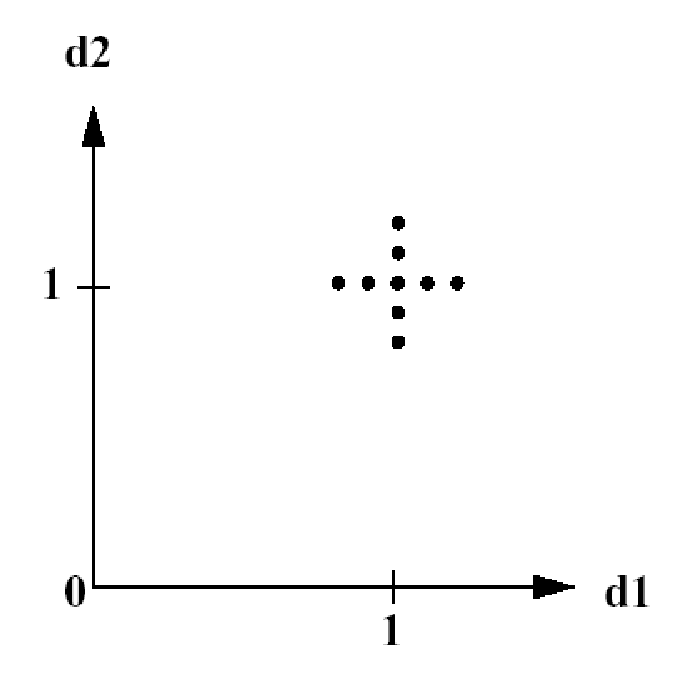
\includegraphics[scale=0.5]{images/centered_pstudy}
  \caption{Example centered parameter study.}
  \label{ps:figure01}
\end{figure}


\section{Multidimensional Parameter Study}\label{ps:multidimensional}

The multidimensional parameter study computes response data sets for
an $n$-dimensional hypergrid of points. Each variable is partitioned
into equally spaced intervals between its upper and lower bounds (see
Section~\ref{ps:overview:bounds}), and each combination of the values
defined by these partitions is evaluated.  As for the vector and
centered studies described in Sections~\ref{ps:vector}
and~\ref{ps:centered}, partitioning occurs using the actual variable
values for continuous and discrete range variables, but occurs within
the space of valid indices for discrete set variables (integer or
real).  The number of function evaluations performed in the study is:
\begin{equation}
  \prod_{i=1}^{n}(\hbox{\texttt{partitions}}_{i}+1)
  \label{ps:equation01}
\end{equation}

The partitions information is specified using the \texttt{partitions}
specification, which provides an integer list of the number of
partitions for each variable (i.e., \texttt{partitions}$_{i}$). Since
the Initial Values will not be used, they need not be specified.

In a two variable example problem with \texttt{d1} $\in$ [0,2] and 
\texttt{d2} $\in$ [0,3] (as defined by the upper and lower bounds 
from the variables specification) and with \texttt{partitions} =
(2,3), the interval [0,2] is divided into two equal-sized partitions
and the interval [0,3] is divided into three equal-sized partitions. 
This two-dimensional grid, shown in Figure~\ref{ps:figure02}, would 
result in the following twelve function evaluations:
\begin{figure}
  \centering
  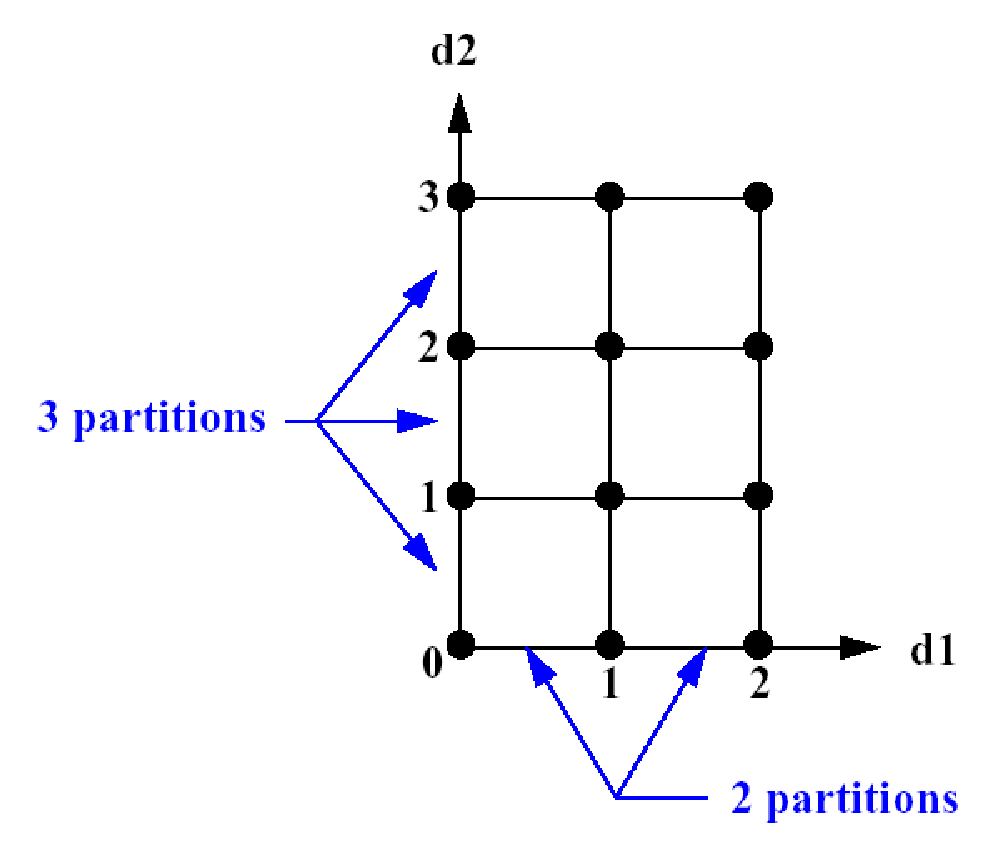
\includegraphics[scale=0.5]{images/multi_d_pstudy}
  \caption{Example multidimensional parameter study}
  \label{ps:figure02}
\end{figure}

\begin{small}
\begin{verbatim}
    Parameters for function evaluation 1:
                          0.0000000000e+00 d1   
                          0.0000000000e+00 d2   
    Parameters for function evaluation 2:
                          1.0000000000e+00 d1   
                          0.0000000000e+00 d2   
    Parameters for function evaluation 3:
                          2.0000000000e+00 d1   
                          0.0000000000e+00 d2   
    Parameters for function evaluation 4:
                          0.0000000000e+00 d1   
                          1.0000000000e+00 d2   
    Parameters for function evaluation 5:
                          1.0000000000e+00 d1   
                          1.0000000000e+00 d2   
    Parameters for function evaluation 6:
                          2.0000000000e+00 d1   
                          1.0000000000e+00 d2   
    Parameters for function evaluation 7:
                          0.0000000000e+00 d1   
                          2.0000000000e+00 d2   
    Parameters for function evaluation 8:
                          1.0000000000e+00 d1   
                          2.0000000000e+00 d2   
    Parameters for function evaluation 9:
                          2.0000000000e+00 d1   
                          2.0000000000e+00 d2   
    Parameters for function evaluation 10:
                          0.0000000000e+00 d1   
                          3.0000000000e+00 d2   
    Parameters for function evaluation 11:
                          1.0000000000e+00 d1   
                          3.0000000000e+00 d2   
    Parameters for function evaluation 12:
                          2.0000000000e+00 d1   
                          3.0000000000e+00 d2
\end{verbatim}
\end{small}

The first example shown in this User's Manual is a multi-dimensional
parameter study. See Section~\ref{tutorial:examples:param_study}.

\section{Parameter Study Usage Guidelines}\label{ps:usage}

Parameter studies, classical design of experiments (DOE),
design/analysis of computer experiments (DACE), and sampling methods
share the purpose of exploring the parameter space.  Parameter Studies
are recommended for simple studies with defined, repetitive structure.
A local sensitivity analysis or an assessment of the
smoothness of a response function is best addressed with a vector or
centered parameter study. A multi-dimensional parameter 
study may be used to generate grid points for plotting response surfaces.
For guidance on DACE and sampling methods, in contrast to parameter 
studies, see Section~\ref{dace:usage} and especially Table~\ref{dace:usage:table},
which clarifies the different purposes of the method types.
 
\section{Example: Vector Parameter Study with Rosenbrock}\label{ps:example:vector}

This section demonstrates a vector parameter study on the Rosenbrock 
test function described in Section~\ref{tutorial:examples:rosenbrock}.  
An example of multidimensional parameter study is shown in 
Section~\ref{tutorial:examples:param_study}.

A vector parameter study is a study between any 
two design points in an \emph{n}-dimensional parameter space.
An input file for the vector parameter study is shown in Figure~
\ref{additional:rosenbrock_vector}. The primary differences
between this input file and the input file for the multidimensional
parameter study are found in the
\emph{variables} and \emph{method} sections. In the variables section,
the keywords for the bounds are removed and replaced with the keyword
\texttt{initial\_point} that specifies the starting point for the
parameter study. In the method section, the
\texttt{vector\_parameter\_study} keyword is used. The
\texttt{final\_point} keyword indicates the stopping point for the
parameter study, and \texttt{num\_steps} specifies the number of steps
taken between the initial and final points in the parameter study.

\begin{figure}[ht!]
  \centering
  \begin{bigbox}
    \begin{small}
      \verbatimtabinput[8]{rosen_ps_vector.in}
    \end{small}
  \end{bigbox}
  \caption{Rosenbrock vector parameter study example: the Dakota input
  file --
see \texttt{Dakota/examples/users/rosen\_ps\_vector.in} }
  \label{additional:rosenbrock_vector}
\end{figure}

Figure~\ref{additional:rosenbrock_vector_graphics}(a) shows the
graphics output created by Dakota. For this study, the simple Dakota
graphics are more useful for visualizing the
results. Figure~\ref{additional:rosenbrock_vector_graphics}(b)
shows the locations of the 11 sample points generated in this study.
It is evident from these figures that the parameter study starts
within the banana-shaped valley, marches up the side of the hill, and
then returns to the valley.

\begin{figure}[htp!]
  \centering
  \begin{tabular}{c}
  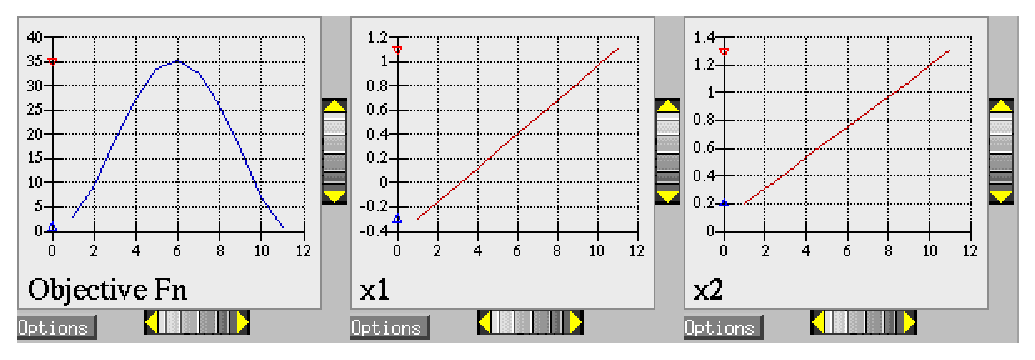
\includegraphics[width=\textwidth]{images/dak_graphics_vector}\\
  (a)\\
  \qquad\\
  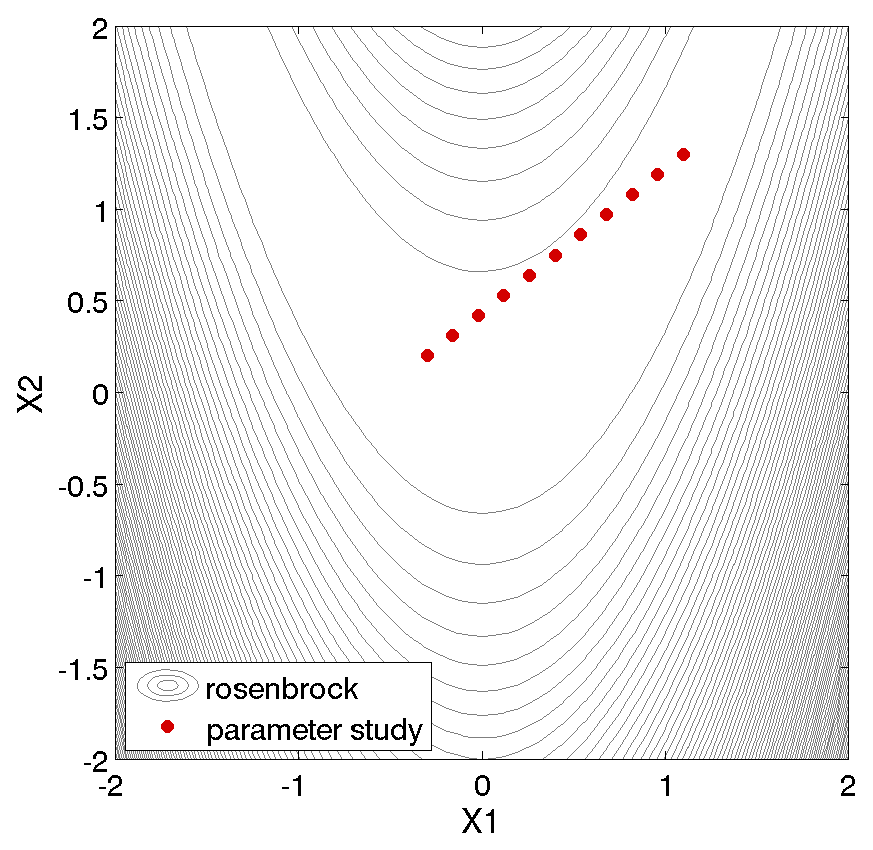
\includegraphics[height=2.5in]{images/rosen_vect_pts} \\
  (b)
  \end{tabular}
  \caption{Rosenbrock vector parameter study example: (a) screen
    capture of the Dakota graphics and (b) location of the design
    points (dots) evaluated.}
  \label{additional:rosenbrock_vector_graphics}
\end{figure}

\chapter{Design of Experiments Capabilities}\label{dace}

\section{Overview}\label{dace:overview}

Classical design of experiments (DoE) methods and the more modern
design and analysis of computer experiments (DACE) methods are both
techniques which seek to extract as much trend data from a parameter
space as possible using a limited number of sample points. Classical
DoE techniques arose from technical disciplines that assumed some
randomness and nonrepeatability in field experiments (e.g.,
agricultural yield, experimental chemistry). DoE approaches such as
central composite design, Box-Behnken design, and full and fractional
factorial design generally put sample points at the extremes of the
parameter space, since these designs offer more reliable trend
extraction in the presence of nonrepeatability. DACE methods are
distinguished from DoE methods in that the nonrepeatability component
can be omitted since computer simulations are involved. In these
cases, space filling designs such as orthogonal array sampling and
Latin hypercube sampling are more commonly employed in order to
accurately extract trend information. Quasi-Monte Carlo sampling
techniques which are constructed to fill the unit hypercube with good
uniformity of coverage can also be used for DACE.

Dakota supports both DoE and DACE techniques. In common usage, only
parameter bounds are used in selecting the samples within the
parameter space. Thus, DoE and DACE can be viewed as special cases of
the more general probabilistic sampling for uncertainty quantification
(see following section), in which the DoE/DACE parameters are treated
as having uniform probability distributions. The DoE/DACE techniques
are commonly used for investigation of global response trends,
identification of significant parameters (e.g., main effects), and as
data generation methods for building response surface approximations.

Dakota includes several approaches sampling and design of experiments,
all implemented in included third-party software libraries. LHS
(Latin hypercube sampling)~\cite{Swi04} is a general-purpose sampling
package developed at Sandia that has been used by the DOE national
labs for several decades. DDACE (distributed design and analysis for
computer experiments) is a more recent package for computer
experiments developed at Sandia Labs~\cite{TonXX}. DDACE provides the
capability for generating orthogonal arrays, Box-Behnken designs,
Central Composite designs, and random designs. The FSUDace (Florida
State University's Design and Analysis of Computer Experiments)
package provides the following sampling techniques: quasi-Monte Carlo
sampling based on Halton or Hammersley sequences, and Centroidal
Voronoi Tessellation. Lawrence Livermore National Lab's PSUADE
(Problem Solving Environment for Uncertainty Analysis and Design
Exploration)~\cite{Ton05} includes several methods for model
exploration, but only the Morris screening method is exposed in
Dakota.

This chapter describes DDACE, FSUDace, and PSUADE, with a focus on
designing computer experiments. Latin Hypercube Sampling, also used in
uncertainty quantification, is discussed in Section~\ref{uq:sampling}.
\begin{comment}
The differences between sampling used in design of experiments and
sampling used in uncertainty quantification is discussed in more
detail in the following paragraphs. In brief, we consider design of
experiment methods to generate sets of uniform random variables on the
interval $[0,1]$. These sets are mapped to the lower/upper bounds of
the problem variables and then the response functions are evaluated at
the sample input points with the goal of characterizing the behavior
of the response functions over the input parameter ranges of
interest. Uncertainty quantification via LHS sampling, in contrast,
involves characterizing the uncertain input variables with probability
distributions such as normal, Weibull, triangular, etc., sampling from
the input distributions, and propagating the input uncertainties to
obtain a cumulative distribution function on the output. There is
significant overlap between design of experiments and sampling. Often,
both techniques can be used to obtain similar results about the
behavior of the response functions and about the relative importance
of the input variables.
\end{comment}

\section{Design of Computer Experiments}\label{dace:background}

What distinguishes design of {\em computer} experiments?  Computer
experiments are often different from physical experiments, such as
those performed in agriculture, manufacturing, or biology. In
physical experiments, one often applies the same \emph{treatment} or
\emph{factor level} in an experiment several times to get an
understanding of the variability of the output when that treatment is
applied. For example, in an agricultural experiment, several fields
(e.g., 8) may be subject to a low level of fertilizer and the same
number of fields may be subject to a high level of fertilizer to see
if the amount of fertilizer has a significant effect on crop
output. In addition, one is often interested in the variability of the
output within a treatment group: is the variability of the crop yields
in the low fertilizer group much higher than that in the high
fertilizer group, or not?

In physical experiments, the process we are trying to examine is stochastic:  
that is, the same treatment may result in different outcomes. 
By contrast, in computer experiments, often we have a deterministic code. 
If we run the code with a particular set of input parameters, the code 
will always produce the same output. There certainly are stochastic codes, 
but the main focus of computer experimentation has been on deterministic codes. 
Thus, in computer experiments we often do not have the need to do replicates 
(running the code with the exact same input parameters several times to see 
differences in outputs). Instead, a major concern in computer experiments is 
to create an experimental design which can sample a high-dimensional space 
in a representative way with a minimum number of samples. 
The number of factors or parameters that we wish to explore in computer 
experiments is usually much higher than physical experiments. 
In physical experiments, one may be interested in varying a few parameters, 
usually five or less, while in computer experiments we often have 
dozens of parameters of interest. Choosing the levels of these parameters 
so that the samples adequately explore the input space is a challenging 
problem. There are many experimental designs and sampling methods 
which address the issue of adequate and representative sample selection. 
%Classical experimental designs which are often used in physical experiments 
%include Central Composite designs and Box-Behnken designs.

There are many goals of running a computer experiment: one may want to 
explore the input domain or the design space and get a better understanding 
of the range in the outputs for a particular domain. Another objective is 
to determine which inputs have the most influence on the output, or how 
changes in the inputs change the output. This is usually called 
\emph{sensitivity analysis}. 
%Another goal is to compare the relative 
%importance of model input uncertainties on the uncertainty in the model 
%outputs, \emph{uncertainty analysis}. 
Another goal is to use the 
sampled input points and their corresponding output to create a 
\emph{response surface approximation} for the computer code. The response 
surface approximation (e.g., a polynomial regression model, a 
Gaussian-process/Kriging model, a neural net) can then be used to emulate 
the computer code. 
Constructing a response surface approximation is particularly important 
for applications where running a computational model is extremely expensive:  
the computer model may take 10 or 20 hours to run on a high performance 
machine, whereas the response surface model may only take a few seconds. 
Thus, one often optimizes the response surface model or uses it within a 
framework such as surrogate-based optimization. Response surface models 
are also valuable in cases where the gradient (first derivative) and/or 
Hessian (second derivative) information required by optimization techniques 
are either not available, expensive to compute, or inaccurate because the 
derivatives are poorly approximated or the function evaluation is itself 
noisy due to roundoff errors. Furthermore, many optimization methods 
require a good initial point to ensure fast convergence or to converge to 
good solutions (e.g. for problems with multiple local minima). Under these 
circumstances, a good design of computer experiment framework coupled with 
response surface approximations can offer great advantages. 

In addition to the sensitivity analysis and response 
surface modeling mentioned above, we also may want to do 
\emph{uncertainty quantification} on a computer model. 
Uncertainty quantification (UQ) refers to taking a particular set of 
distributions on the inputs, and propagating them through the model to 
obtain a distribution on the outputs. For example, if input parameter A 
follows a normal with mean 5 and variance 1, the computer produces a random 
draw from that distribution. If input parameter B follows a weibull 
distribution with alpha = 0.5 and beta = 1, the computer produces a random 
draw from that distribution. When all of the uncertain variables have 
samples drawn from their input distributions, we run the model with the 
sampled values as inputs. We do this repeatedly to build up a distribution 
of outputs. We can then use the cumulative distribution function of the 
output to ask questions such as:  what is the probability that the output is 
greater than 10?   What is the 99th percentile of the output?  

Note that sampling-based uncertainty quantification and design of
computer experiments are very similar. \emph{There is significant
overlap} in the purpose and methods used for UQ and for DACE. We have
attempted to delineate the differences within Dakota as follows: we
use the methods DDACE, FSUDACE, and PSUADE primarily for design of
experiments, where we are interested in understanding the main effects
of parameters and where we want to sample over an input domain to
obtain values for constructing a response surface. We use the
nondeterministic sampling methods \texttt{(sampling)} for
uncertainty quantification, where we are propagating specific input
distributions and interested in obtaining (for example) a cumulative
distribution function on the output. If one has a problem with no
distributional information, we recommend starting with a design of
experiments approach. Note that DDACE, FSUDACE, and PSUADE currently
do \emph{not} support distributional information: they take an upper
and lower bound for each uncertain input variable and sample within
that. The uncertainty quantification methods in
\texttt{sampling} (primarily Latin Hypercube sampling) offer the
capability to sample from many distributional types. The distinction
between UQ and DACE is somewhat arbitrary: both approaches often can
yield insight about important parameters and both can determine sample
points for response surface approximations.

Three software packages are available in Dakota for design of computer
experiments, DDACE (developed at Sandia Labs), FSUDACE (developed at
Florida State University), and PSUADE (LLNL).

\section{DDACE}\label{dace:ddace}

The Distributed Design and Analysis of Computer Experiments (DDACE)
package includes both classical design of experiments
methods~\cite{TonXX} and stochastic sampling methods. The classical
design of experiments methods in DDACE are central composite design
(CCD) and Box-Behnken (BB) sampling. A grid-based sampling
(full-factorial) method is also available. The stochastic methods are
orthogonal array sampling~\cite{Koe96} (which permits main effects
calculations), Monte Carlo (random) sampling, Latin hypercube
sampling, and orthogonal array-Latin hypercube sampling. While DDACE
LHS supports variables with normal or uniform distributions, only
uniform are supported through Dakota. Also DDACE does not allow
enforcement of user-specified correlation structure among the
variables.

The sampling methods in DDACE can be used alone or in conjunction with
other methods. For example, DDACE sampling can be used with both
surrogate-based optimization and optimization under uncertainty
advanced methods. See Figure~\ref{adv_models:figure09} for an example
of how the DDACE settings are used in Dakota.

%More information on DDACE is available on the web at:
%\url{http://csmr.ca.sandia.gov/projects/ddace}

The following sections provide more detail about the sampling 
methods available for design of experiments in DDACE. 

\subsection{Central Composite Design}\label{dace:ccd}

A Box-Wilson Central Composite Design, commonly called a central
composite design (CCD), contains an embedded factorial or fractional
factorial design with center points that is augmented with a group of
'star points' that allow estimation of curvature. If the distance
from the center of the design space to a factorial point is $\pm$1
unit for each factor, the distance from the center of the design space
to a star point is $\pm\alpha$ with $\mid\alpha\mid > 1$. The precise
value of $\alpha$ depends on certain properties desired for the design and on
the number of factors involved. The CCD design is specified in Dakota
with the method command \texttt{dace central\_composite}.

As an example, with two input variables or factors, each having two 
levels, the factorial design is shown in Table~\ref{dace:table01} . 

\begin{table}[ht]
 \caption{Simple Factorial Design}
 \label{dace:table01}	
 \begin{center}
  \begin{tabular}{c|c}
  \hline
  Input 1            & Input 2         \\ \hline \hline 
  -1                 & -1             \\ \hline 
  -1                 & +1           \\ \hline
  +1                 & -1      \\ \hline
  +1                 & +1        \\ \hline
  \end{tabular}
\end{center}
\end{table}


With a CCD, the design in Table~\ref{dace:table01} would be augmented 
with the following points shown in Table~\ref{dace:table02} 
if $\alpha$ = 1.3. These points define a circle around the original  
factorial design.

\begin{table}[ht]
 \caption{Additional Points to make the factorial design a CCD}
 \label{dace:table02}
 \begin{center}
  \begin{tabular}{c|c}
  \hline
  Input 1            & Input 2         \\ \hline \hline 
  0                 & +1.3             \\ \hline 
  0                 & -1.3           \\ \hline
  1.3                 & 0     \\ \hline
  -1.3                 & 0       \\ \hline
  0                  & 0          \\ \hline
  \end{tabular}
\end{center}
\end{table}

Note that the number of sample points specified in a CCD,\texttt{samples},
is a function of the number of variables in the problem: 

\[
samples = 1 + 2*NumVar + 2^{NumVar}
\]

\subsection{Box-Behnken Design}\label{dace:bb}

The Box-Behnken design is similar to a Central Composite design, with
some differences. The Box-Behnken design is a quadratic design in
that it does not contain an embedded factorial or fractional factorial
design. In this design the treatment combinations are at the midpoints
of edges of the process space and at the center, as compared with CCD
designs where the extra points are placed at 'star points' on a circle
outside of the process space. Box-Behken designs are rotatable (or
near rotatable) and require 3 levels of each factor. The designs have
limited capability for orthogonal blocking compared to the central
composite designs. Box-Behnken requires fewer runs than CCD for 3
factors, but this advantage goes away as the number of factors
increases. The Box-Behnken design is specified in Dakota with the
method command \texttt{dace box\_behnken}.

Note that the number of sample points specified in a Box-Behnken design,
\texttt{samples}, is a function of the number of variables in the problem: 

\[
samples = 1 + 4*NumVar + (NumVar-1)/2
\]

\subsection{Orthogonal Array Designs}\label{dace:oas}

Orthogonal array (OA) sampling is a widely used technique for 
running experiments and systematically testing factor effects~\cite{Hed99}. 
An orthogonal array sample can be described as a 4-tuple $(m,n,s,r)$,
where $m$ is the number of sample points, $n$ is the number of input variables, 
$s$ is the number of symbols, and $r$ is the strength of the orthogonal array. 
The number of sample points, $m$, must be a multiple of the number of symbols, 
$s$. The number of symbols refers to the number of levels per input variable. 
The strength refers to the number of columns where we are guaranteed to 
see all the possibilities an equal number of times.

For example, Table~\ref{dace:table03} shows an orthogonal array of strength 2 for $m$ = 8, with 7 variables:

\begin{table}[ht]
 \caption{Orthogonal Array for Seven Variables}
 \label{dace:table03}
 \begin{center}
  \begin{tabular}{c|c|c|c|c|c|c}
  \hline
  Input 1 & Input 2 & Input 3 & Input 4 & Input 5 & Input 6 & Input 7\\ \hline \hline 
0 & 	0 &	0 &	0 & 	0 &	0 &	0  \\ \hline
0 &	0 &	0 &	1 &	1 &	1 &	1   \\ \hline
0 &	1 & 	1 & 	0 & 	0 &	1 &	1   \\ \hline
0 &	1 &	1 &	1 &	1 &	0 &	0    \\ \hline
1 &	0 &	1 &	0 &	1 &	0 &	1   \\ \hline
1 &	0 &	1 &	1 &	0 &	1 &	0 \\ \hline
1 &	1 &	0 &	0 &	1 &	1 &	0 \\ \hline
1 &	1 &	0 &	1 &	0 &	0 &	1 \\ \hline

  \end{tabular}
\end{center}
\end{table}


If one picks any two columns, say the first and the third, note that 
each of the four possible rows we might see there,
0 0,       0 1,       1 0,       1 1,
appears exactly the same number of times, twice in this case.

DDACE creates orthogonal arrays of strength 2. Further, 
the OAs generated by DDACE do not treat the factor levels as one 
fixed value (0 or 1 in the above example). Instead, once a level 
for a variable is determined in the array,  DDACE 
samples a random variable from within that level.
The orthogonal array design is specified in 
Dakota with the method command \texttt{dace oas}. 

The orthogonal array method in DDACE is the only method that 
allows for the calculation of main effects, specified with the 
command \texttt{main\_effects}. Main effects is a sensitivity analysis 
method which identifies the input variables that have the most 
influence on the output. In main effects, the idea is to look 
at the mean of the response function when variable A (for example) 
is at level 1 vs. when variable A is at level 2 or level 3. 
If these mean responses of the output are statistically significantly 
different at different levels of variable A, this is an indication that 
variable A has a significant effect on the response. 
The orthogonality of the columns is critical in performing 
main effects analysis, since the column orthogonality means 
that the effects of the other variables 'cancel out' when 
looking at the overall effect from one variable at its different 
levels. There are ways of developing orthogonal arrays to calculate 
higher order interactions, such as two-way interactions (what 
is the influence of Variable A * Variable B on the output?), but this is 
not available in DDACE currently. At present, one way interactions 
are supported in the calculation of orthogonal array main effects within DDACE.
The main effects are presented as a series of ANOVA tables. 
For each objective function and constraint, the decomposition of variance 
of that objective or constraint is presented as a function of the 
input variables. The p-value in the ANOVA table is used to indicate 
if the input factor is significant. The p-value is the probability that 
you would have obtained samples more extreme than you did if the input 
factor has no effect on the response. For example, if you set a level 
of significance at 0.05 for your p-value, and the actual p-value is 0.03, 
then the input factor has a significant effect on the response. 

\subsection{Grid Design}\label{dace:grid}

In a grid design, a grid is placed over the input variable space. 
This is very similar to a multi-dimensional parameter study where 
the samples are taken over a set of partitions on each variable 
(see Section~\ref{ps:multidimensional}). The main difference is 
that in grid sampling, a small random perturbation is added 
to each sample value so that the grid points are not on a perfect grid. 
This is done to help capture certain features in the output such as periodic
functions. A purely structured grid, with the samples exactly on the grid 
points, has the disadvantage of not being able to capture important features 
such as periodic functions with relatively high frequency (due to aliasing). 
Adding a random perturbation to the grid samples helps remedy this problem.

Another disadvantage with grid sampling is that the number of sample points 
required depends exponentially on the input dimensions. In grid sampling, 
the number of samples is the number of symbols (grid partitions) raised 
to the number of variables. For example, if there are 2 variables, each 
with 5 partitions, the number of samples would be $5^2$. In this 
case, doubling the number of variables squares the sample size. 
The grid design is specified in 
Dakota with the method command \texttt{dace grid}.

\subsection{Monte Carlo Design}\label{dace:mc}

Monte Carlo designs simply involve pure Monte-Carlo random sampling 
from uniform distributions between the lower and upper bounds on each 
of the input variables. Monte Carlo designs, specified by 
\texttt{dace random}, are a way to generate a set of random samples 
over an input domain.

\subsection{LHS Design}\label{dace:lhs}

DDACE offers the capability to generate Latin Hypercube designs. 
For more information on Latin Hypercube sampling, see 
Section~\ref{uq:sampling}. Note that the version of LHS in DDACE 
generates uniform samples (uniform between the variable bounds). 
The version of LHS offered with nondeterministic sampling can generate 
LHS samples according to a number of distribution types, including 
normal, lognormal, weibull, beta, etc. To specify the DDACE version 
of LHS, use the method command \texttt{dace lhs}.

\subsection{OA-LHS Design}\label{dace:oalhs}

DDACE offers a hybrid design which is combination of an orthogonal
array and a Latin Hypercube sample. This design is specified with the
method command \texttt{dace oa\_lhs}. This design has the advantages
of both orthogonality of the inputs as well as stratification of the
samples (see~\cite{Owe92}).

\section{FSUDace}\label{dace:fsudace}

The Florida State University Design and Analysis of Computer
Experiments (FSUDace) package provides quasi-Monte Carlo sampling
(Halton and Hammersley) and Centroidal Voronoi Tessellation (CVT)
methods. All three methods natively generate sets of uniform random
variables on the interval $[0,1]$ (or in Dakota, on user-specified
uniform intervals).

The quasi-Monte Carlo and CVT methods are designed with the goal of
low discrepancy. Discrepancy refers to the nonuniformity of the sample
points within the unit hypercube. Low discrepancy sequences tend to
cover the unit hypercube reasonably uniformly. Quasi-Monte Carlo
methods produce low discrepancy sequences, especially if one is
interested in the uniformity of projections of the point sets onto
lower dimensional faces of the hypercube (usually 1-D: how well do the
marginal distributions approximate a uniform?) CVT does very well
volumetrically: it spaces the points fairly equally throughout the
space, so that the points cover the region and are isotropically
distributed with no directional bias in the point placement. There are
various measures of volumetric uniformity which take into account the
distances between pairs of points, regularity measures, etc. Note that
CVT does not produce low-discrepancy sequences in lower dimensions,
however: the lower-dimension (such as 1-D) projections of CVT can have
high discrepancy.

The quasi-Monte Carlo sequences of Halton and Hammersley are
deterministic sequences determined by a set of prime bases.
A Halton design is specified in Dakota with the method command 
\texttt{fsu\_quasi\_mc halton}, and the Hammersley design is 
specified with the command \texttt{fsu\_quasi\_mc hammersley}.
For more details about the input specification, see the Reference Manual.
CVT points tend to arrange themselves in a pattern
of cells that are roughly the same shape. To produce CVT
points, an almost arbitrary set of initial points is chosen, and then
an internal set of iterations is carried out. These iterations
repeatedly replace the current set of sample points by an estimate of
the centroids of the corresponding Voronoi subregions~\cite{Du99}.
A CVT design is specified in Dakota with the method command
\texttt{fsu\_cvt}.

The methods in FSUDace are useful for design of experiments because 
they provide good coverage of the input space, thus allowing global 
sensitivity analysis. 

\section{PSUADE MOAT}\label{dace:psuade}

PSUADE (Problem Solving Environment for Uncertainty Analysis and
Design Exploration) is a Lawrence Livermore National Laboratory tool
for metamodeling, sensitivity analysis, uncertainty quantification,
and optimization. Its features include non-intrusive and parallel
function evaluations, sampling and analysis methods, an integrated
design and analysis framework, global optimization, numerical
integration, response surfaces (MARS and higher order regressions),
graphical output with Pgplot or Matlab, and fault
tolerance~\cite{Ton05}. Dakota includes a prototype interface to its
Morris One-At-A-Time (MOAT) screening method, a valuable tool for
global sensitivity (including interaction) analysis.

The Morris One-At-A-Time method, originally proposed by
M.~D. Morris~\cite{Mor91}, is a screening method, designed to explore
a computational model to distinguish between input variables that have
negligible, linear and additive, or nonlinear or interaction effects
on the output. The computer experiments performed consist of
individually randomized designs which vary one input factor at a time
to create a sample of its elementary effects.

With MOAT, each dimension of a $k-$dimensional input space is
uniformly partitioned into $p$ levels, creating a grid of $p^k$ points
${\bf x} \in \mathbb{R}^k$ at which evaluations of the model $y({\bf
x})$ might take place. An elementary effect corresponding to input
$i$ is computed by a forward difference
\begin{equation}
d_i({\bf x}) = \frac{y({\bf x} + \Delta {\bf e}_i) - y({\bf x})}{\Delta},
\end{equation}
where $e_i$ is the $i^{\mbox{\scriptsize th}}$ coordinate vector, and
the step $\Delta$ is typically taken to be large (this is not intended
to be a local derivative approximation). In the present
implementation of MOAT, for an input variable scaled to $[0,1]$,
$\Delta = \frac{p}{2(p-1)}$, so the step used to find elementary
effects is slightly larger than half the input range.

The distribution of elementary effects $d_i$ over the input space
characterizes the effect of input $i$ on the output of interest.
After generating $r$ samples from this distribution, their mean,
\begin{equation}
\mu_i = \frac{1}{r}\sum_{j=1}^{r}{d_i^{(j)}},
\end{equation}
modified mean
\begin{equation}
\mu_i^* = \frac{1}{r}\sum_{j=1}^{r}{|d_i^{(j)}|},
\end{equation}
(using absolute value) and standard deviation
\begin{equation}
\sigma_i = \sqrt{ \frac{1}{r}\sum_{j=1}^{r}{ \left(d_i^{(j)} - \mu_i
\right)^2} }
\end{equation}
are computed for each input $i$. The mean and modified mean give an
indication of the overall effect of an input on the output. Standard
deviation indicates nonlinear effects or interactions, since it is an
indicator of elementary effects varying throughout the input space.

The MOAT method is selected with method keyword {\tt psuade\_moat} as
shown in the sample Dakota input deck in Figure~\ref{FIG:moat_input}.
The number of samples ({\tt samples}) must be a positive integer
multiple of (number of continuous design variables $k$ + 1) and will
be automatically adjusted if misspecified. The number of partitions
({\tt partitions}) applies to each variable being studied and must be
odd (the number of MOAT levels $p$ per variable is partitions + 1,
similar to Dakota multidimensional parameter studies). This will also
be adjusted at runtime as necessary. Finite user-specified lower and
upper bounds are required and will be scaled as needed by the method.
For more information on use of MOAT sampling, see the Morris example
in Section~\ref{additional:morris}, or Saltelli, et al.~\cite{Sal04}.

\begin{figure}
  \centering \begin{bigbox} \begin{small}
  \verbatimtabinput[8]{morris_ps_moat.in} \end{small} \end{bigbox}
\caption{Dakota input file showing the Morris One-at-a-Time method --
see {\tt Dakota/examples/users/morris\_ps\_moat.in} }
\label{FIG:moat_input}
\end{figure}

\section{Sensitivity Analysis}\label{dace:sa}

\subsection{Sensitivity Analysis Overview}\label{dace:sa:overview}

In many engineering design applications, sensitivity analysis
techniques and parameter study methods are useful in identifying which
of the design parameters have the most influence on the response
quantities. This information is helpful prior to an optimization study
as it can be used to remove design parameters that do not strongly
influence the responses. In addition, these techniques can provide
assessments as to the behavior of the response functions (smooth or
nonsmooth, unimodal or multimodal) which can be invaluable in
algorithm selection for optimization, uncertainty quantification, and
related methods. In a post-optimization role, sensitivity information
is useful is determining whether or not the response functions are
robust with respect to small changes in the optimum design point.

In some instances, the term sensitivity analysis is used in a local
sense to denote the computation of response derivatives at a point.
These derivatives are then used in a simple analysis to make design
decisions. Dakota supports this type of study through numerical
finite-differencing or retrieval of analytic gradients computed within
the analysis code. The desired gradient data is specified in the
responses section of the Dakota input file and the collection of this
data at a single point is accomplished through a parameter study
method with no steps. This approach to sensitivity analysis should be
distinguished from the activity of augmenting analysis codes to
internally compute derivatives using techniques such as direct or
adjoint differentiation, automatic differentiation (e.g., ADIFOR), or
complex step modifications. These sensitivity augmentation activities
are completely separate from Dakota and are outside the scope of this
manual. However, once completed, Dakota can utilize these analytic
gradients to perform optimization, uncertainty quantification, and
related studies more reliably and efficiently.

In other instances, the term sensitivity analysis is used in a more
global sense to denote the investigation of variability in the
response functions. Dakota supports this type of study through
computation of response data sets (typically function values only, but
all data sets are supported) at a series of points in the parameter
space. The series of points is defined using either a vector, list,
centered, or multidimensional parameter study method. For example, a
set of closely-spaced points in a vector parameter study could be used
to assess the smoothness of the response functions in order to select
a finite difference step size, and a set of more widely-spaced points
in a centered or multidimensional parameter study could be used to
determine whether the response function variation is likely to be
unimodal or multimodal. See Chapter~\ref{ps} for additional
information on these methods. These more global approaches to
sensitivity analysis can be used to obtain trend data even in
situations when gradients are unavailable or unreliable, and they are
conceptually similar to the design of experiments methods and sampling
approaches to uncertainty quantification described in the following
sections.

\subsection{Assessing Sensitivity with DACE}\label{dace:sa:assessing}

Like parameter studies (see Chapter~\ref{ps}), the DACE techniques are
useful for characterizing the behavior of the response functions of
interest through the parameter ranges of interest. In addition to
direct interrogation and visualization of the sampling results, a
number of techniques have been developed for assessing the parameters
which are most influential in the observed variability in the response
functions. One example of this is the well-known technique of scatter
plots, in which the set of samples is projected down and plotted
against one parameter dimension, for each parameter in turn. Scatter
plots with a uniformly distributed cloud of points indicate parameters
with little influence on the results, whereas scatter plots with a
defined shape to the cloud indicate parameters which are more
significant. Related techniques include analysis of variance
(ANOVA)~\cite{Mye95} and main effects analysis, in which the parameters
which have the greatest influence on the results are identified from
sampling results. Scatter plots and ANOVA may be accessed through
import of Dakota tabular results (see Section~\ref{output:tabular})
into external statistical analysis programs such as S-plus, Minitab,
etc.

Running any of the design of experiments or sampling methods allows
the user to save the results in a tabular data file, which then can be
read into a spreadsheet or statistical package for further analysis.
In addition, we have provided some functions to help determine the
most important variables.

We take the definition of uncertainty analysis from~\cite{Sal04}: 
``The study of how uncertainty in the output of a model can be 
apportioned to different sources of uncertainty in the model input.''

As a default, Dakota provides correlation analyses when running LHS.
Correlation tables are printed with the simple, partial, and rank
correlations between inputs and outputs. These can be useful to get a
quick sense of how correlated the inputs are to each other, and how
correlated various outputs are to inputs. The correlation analyses are
explained further in Chapter~\ref{uq:sampling}.

We also have the capability to calculate sensitivity indices through
Variance-based Decomposition (VBD). Variance-based decomposition 
is a global sensitivity method that summarizes how the uncertainty 
in model output can be apportioned to uncertainty in individual 
input variables. VBD uses two primary measures, the main effect 
sensitivity index $S_{i}$ and the total effect index $T_{i}$. The 
main effect sensitivity 
index corresponds to the fraction of the uncertainty in the output, $Y$, 
that can be attributed to input $x_{i}$ alone. The total effects index 
corresponds to the fraction of the uncertainty in 
the output, $Y$, that can be attributed to input $x_{i}$ and its 
interactions with other variables. The main effect sensitivity index
compares the variance of the conditional expectation
$Var_{x_{i}}[E(Y|x_{i})]$ against the total variance $Var(Y)$.
Formulas for the indices are: 

\begin{equation}
S_{i}=\frac{Var_{x_{i}}[E(Y|x_{i})]}{Var(Y)} \label{eq:VBD_Si}
\end{equation}

and 
\begin{equation}
T_{i}=\frac{E(Var(Y|x_{-i}))}{Var(Y)}=\frac{Var(Y)-Var(E[Y|x_{-i}])}{Var(Y)} \label{eq:VBD_Ti}
\end{equation}

where $Y=f({\bf x})$ and ${x_{-i}=(x_{1},...,x_{i-1},x_{i+1},...,x_{m})}$.

The calculation of $S_{i}$ and $T_{i}$ requires the evaluation of 
m-dimensional integrals which are typically approximated by Monte-Carlo 
sampling. More details on the
calculations and interpretation of the sensitivity indices can be
found in~\cite{Sal04}. In Dakota version 5.1, we have 
improved calculations for the calculation of the $S_{i}$ and $T_{i}$ 
indices when using sampling. The implementation details of these 
calculatiosn are provided in~\cite{Weirs10}. 
VBD can be specified for any of the sampling or DACE methods using the 
command \texttt{variance\_based\_decomposition}.
Note that VBD is extremely computationally intensive when using sampling 
since replicated sets of sample values are evaluated. If the
user specified a number of samples, $N$, and a number of
nondeterministic variables, $M$, variance-based decomposition
requires the evaluation of $N(M+2)$ samples. To obtain
sensitivity indices that are reasonably accurate, we recommend that
$N$, the number of samples, be at least one hundred and
preferably several hundred or thousands. Because of the computational
cost, variance-based decomposition is turned off as a default
for sampling or DACE. Another alternative, however, is to obtain 
these indices using one of the stochastic expansion methods 
described in Section~\ref{uq:expansion}. The calculation 
of the indices using expansion methods is much more efficient 
since the VBD indices are analytic functions of the coefficients 
in the stochastic expansion. The paper by Weirs et al.~\cite{Weirs10}
compares different methods for calculating the sensitivity 
indices for nonlinear problems with significant interaction effects.

In terms of interpretation of the sensitivity indices, a larger value of
the sensitivity index, $S_{i}$,
means that the uncertainty in the input variable $i$ has a
larger effect on the variance of the output. Note that the 
sum of the main effect indices will be less than or equal to one. 
If the sum of the main effect indices is much less than one, 
it indicates that there are significant two-way, three-way, or higher
order interactions that contribute significantly to the variance. 
There is no requirement that the sum of the total effect indices 
is one:  in most cases, the sum of the total effect indices will be 
greater than one. An example of the Main and Total effects 
indices as calculated by Dakota using sampling is shown 
in Figure~\ref{fig:dace:vbd}

\begin{figure}[ht!]
\centering
\begin{bigbox}
\begin{small}
\begin{verbatim}
Global sensitivity indices for each response function:
response_fn_1 Sobol indices:
                                  Main             Total
                      4.7508913283e-01  5.3242162037e-01 uuv_1
                      3.8112392892e-01  4.9912486515e-01 uuv_2
\end{verbatim}
\end{small}
\end{bigbox}
\caption{Dakota output for Variance-based Decomposition} 
\label{fig:dace:vbd}
\end{figure}

Finally, we have the capability to calculate a set of quality metrics 
for a particular input sample. These quality metrics measure 
various aspects relating to the volumetric spacing of the samples: 
are the points equally spaced, do they cover the region, are they 
isotropically distributed, do they have directional bias, etc.? 
The quality metrics are explained in more detail in the Reference Manual.

\section{DOE Usage Guidelines}\label{dace:usage}

Parameter studies, classical design of experiments (DOE),
design/analysis of computer experiments (DACE), and sampling methods
share the purpose of exploring the parameter space. When a global
space-filling set of samples is desired, then the DOE, DACE, and
sampling methods are recommended. These techniques are useful for
scatter plot and variance analysis as well as surrogate model
construction. 

The distinction between DOE and DACE methods is that the
former are intended for physical experiments containing an element of
nonrepeatability (and therefore tend to place samples at the extreme
parameter vertices), whereas the latter are intended for repeatable
computer experiments and are more space-filling in nature. 

The distinction between DOE/DACE and sampling is drawn based on the
distributions of the parameters. DOE/DACE methods typically assume
uniform distributions, whereas the sampling approaches in Dakota
support a broad range of probability distributions. 

To use \texttt{sampling} in design of experiments mode (as opposed to
uncertainty quantification mode), an active view override (e.g.,
\texttt{active all}) can be included in the variables specification
(see Section~\ref{variables:mixedview}) of the Dakota input file.

Design of experiments method selection recommendations are summarized
in Table~\ref{dace:usage:table}.

\begin{table}[hbp]
\centering
\caption{Guidelines for selection of parameter study, DOE, DACE, and
sampling methods.}
\label{dace:usage:table}\vspace{2mm}
\begin{tabular}{|c|c|c|}
\hline
\textbf{Method} & \textbf{Applications} & \textbf{Applicable Methods} \\
\textbf{Classification} & & \\
\hline
parameter study & sensitivity analysis,                       & centered\_parameter\_study, \\
                & directed parameter space investigations     & list\_parameter\_study, \\
                &                                             & multidim\_parameter\_study, \\
                &                                             & vector\_parameter\_study \\
                   &                                             & \\
\hline
classical design & physical experiments                       & dace (box\_behnken, \\
of experiments   & (parameters are uniformly distributed)     & central\_composite) \\
                   &                                             & \\
\hline
design of computer & variance analysis,                       & dace (grid, random,
                                                                oas, lhs, oa\_lhs), \\
experiments        & space filling designs                    & fsu\_quasi\_mc (halton, 
                                                                hammersley), \\
                   & (parameters are uniformly distributed)   & fsu\_cvt, psuade\_moat \\
                   &                                             & \\
\hline
sampling           & space filling designs                    & sampling (Monte Carlo or LHS) \\
                   & (parameters have general probability distributions) & with optional active view override \\
                   &                                             & \\
\hline
\end{tabular}
\end{table}

\chapter{Uncertainty Quantification Capabilities}\label{uq}

\section{Overview}\label{uq:overview}

Uncertainty quantification (UQ) is the process of determining the
effect of input uncertainties on response metrics of interest.  These
input uncertainties may be characterized as either aleatory
uncertainties, which are irreducible variabilities inherent in nature,
or epistemic uncertainties, which are reducible uncertainties
resulting from a lack of knowledge.  Since sufficient data is
generally available for aleatory uncertainties, probabilistic methods
are commonly used for computing response distribution statistics based
on input probability distribution specifications.  Conversely, for
epistemic uncertainties, data is generally sparse, making the use of
probability distribution assertions questionable and typically leading
to nonprobabilistic methods based on interval specifications.

DAKOTA contains capabilities for performing nondeterministic analysis.  
The methods for uncertainty quantification in DAKOTA have been developed 
by a group of researchers at Sandia Labs, in conjunction with collaborators in
academia~\cite{Gha99,Gha91,Eld05,Tang10a}. 
%In addition, future extensions to the DDACE package will make it 
%applicable to general UQ problems, which will augment the DAKOTA/UQ 
%capabilities.
%Uncertainty quantification methods (also referred to as
%nondeterministic analysis methods) in the DAKOTA/UQ system involve the
%computation of probabilistic information about response functions
%based on sets of simulations taken from the specified probability
%distributions for uncertain parameters. That is, 
These methods perform a forward uncertainty propagation in which
probability or interval information for input parameters is mapped to
probability or interval information for output response functions. The
$m$ functions in the DAKOTA response data set are interpreted as $m$
general response functions by the DAKOTA methods (with no specific
interpretation of the functions as for optimization and least squares).

Within the variables specification, uncertain variable descriptions
are employed to define the parameter probability distributions (see
Section~\ref{variables:uncertain}). The continuous aleatory
distribution types include: normal (Gaussian), lognormal, uniform,
loguniform, triangular, exponential, beta, gamma, gumbel, frechet,
weibull, and histogram bin.  The discrete aleatory distribution types
include: poisson, binomial, negative binomial, geometric,
hypergeometric, and histogram point.  The epistemic distribution type
is interval.  When gradient and/or Hessian information is used in an
uncertainty assessment, derivative components are normally computed
with respect to the active continuous variables, or in this case, the
\emph{continuous uncertain variables} (aleatory, epistemic, 
or both, excluding \texttt{all\_variables} mode; see 
Section~\ref{responses:active}).

\section{Sampling Methods}\label{uq:sampling}

Sampling techniques are selected using the \texttt{sampling}
method selection. This method generates sets of samples according to
the probability distributions of the uncertain variables and maps them
into corresponding sets of response functions, where the number of
samples is specified by the \texttt{samples} integer specification.
Means, standard deviations, coefficients of variation (COVs), and 95\%
confidence intervals are computed for the response functions.
Probabilities and reliabilities may be computed for 
\texttt{response\_levels} specifications, and response levels may be
computed for either \texttt{probability\_levels} or
\texttt{reliability\_levels} specifications (refer to the Method
Commands chapter in the DAKOTA Reference Manual~\cite{RefMan} for
additional information).

Currently, traditional Monte Carlo (MC) and Latin hypercube sampling
(LHS) are supported by DAKOTA and are chosen by specifying
\texttt{sample\_type} as \texttt{random} or \texttt{lhs}. In Monte
Carlo sampling, the samples are selected randomly according to the
user-specified probability distributions. Latin hypercube sampling is
a stratified sampling technique for which the range of each uncertain
variable is divided into $N_{s}$ segments of equal probability, where
$N_{s}$ is the number of samples requested. The relative lengths of
the segments are determined by the nature of the specified probability
distribution (e.g., uniform has segments of equal width, normal has
small segments near the mean and larger segments in the tails). For
each of the uncertain variables, a sample is selected randomly from
each of these equal probability segments.  These $N_{s}$ values for
each of the individual parameters are then combined in a shuffling
operation to create a set of $N_{s}$ parameter vectors with a
specified correlation structure. A feature of the resulting sample set
is that 
\emph{every row and column in the hypercube of partitions has exactly one sample}.
Since the total number of samples is exactly equal
to the number of partitions used for each uncertain variable, an
arbitrary number of desired samples is easily accommodated (as
compared to less flexible approaches in which the total number of
samples is a product or exponential function of the number of
intervals for each variable, i.e., many classical design of
experiments methods).

Advantages of sampling-based methods include their relatively simple
implementation and their independence from the scientific disciplines
involved in the analysis. The main drawback of these techniques is the
large number of function evaluations needed to generate converged
statistics, which can render such an analysis computationally very
expensive, if not intractable, for real-world engineering
applications. LHS techniques, in general, require fewer samples than
traditional Monte Carlo for the same accuracy in statistics, but they
still can be prohibitively expensive. For further information on the
method and its relationship to other sampling techniques, one is
referred to the works by McKay, et al.~\cite{Mck79}, Iman and
Shortencarier~\cite{Ima84}, and Helton and Davis~\cite{Hel00}.
Note that under certain separability conditions associated with the 
function to be sampled,
Latin hypercube sampling provides a more accurate estimate of the mean
value than does random sampling. That is, given an equal number of
samples, the LHS estimate of the mean will have less variance than the
mean value obtained through random sampling.

Figure~\ref{dace:figure01} demonstrates Latin hypercube sampling on a
two-variable parameter space. Here, the range of both parameters,
$x_1$ and $x_2$, is $[0,1]$. Also, for this example both $x_1$
and $x_2$ have uniform statistical distributions.  For Latin
hypercube sampling, the range of each parameter is divided into $p$
``bins'' of equal probability. For parameters with uniform
distributions, this corresponds to partitions of equal size. For $n$
design parameters, this partitioning yields a total of $p^{n}$ bins in
the parameter space.  Next, $p$ samples are randomly selected in the
parameter space, with the following restrictions: (a) each sample is
randomly placed inside a bin, and (b) for all one-dimensional
projections of the $p$ samples and bins, there will be one and only
one sample in each bin.  In a two-dimensional example such as that
shown in Figure~\ref{dace:figure01}, these LHS rules guarantee that
only one bin can be selected in each row and column. For $p=4$, there
are four partitions in both $x_1$ and $x_2$. This gives a total of
16 bins, of which four will be chosen according to the criteria
described above. Note that there is more than one possible arrangement
of bins that meet the LHS criteria.  The dots in
Figure~\ref{dace:figure01} represent the four sample sites in this
example, where each sample is randomly located in its bin.  There is
no restriction on the number of bins in the range of each parameter,
however, all parameters must have the same number of bins.

\begin{figure}
  \centering
  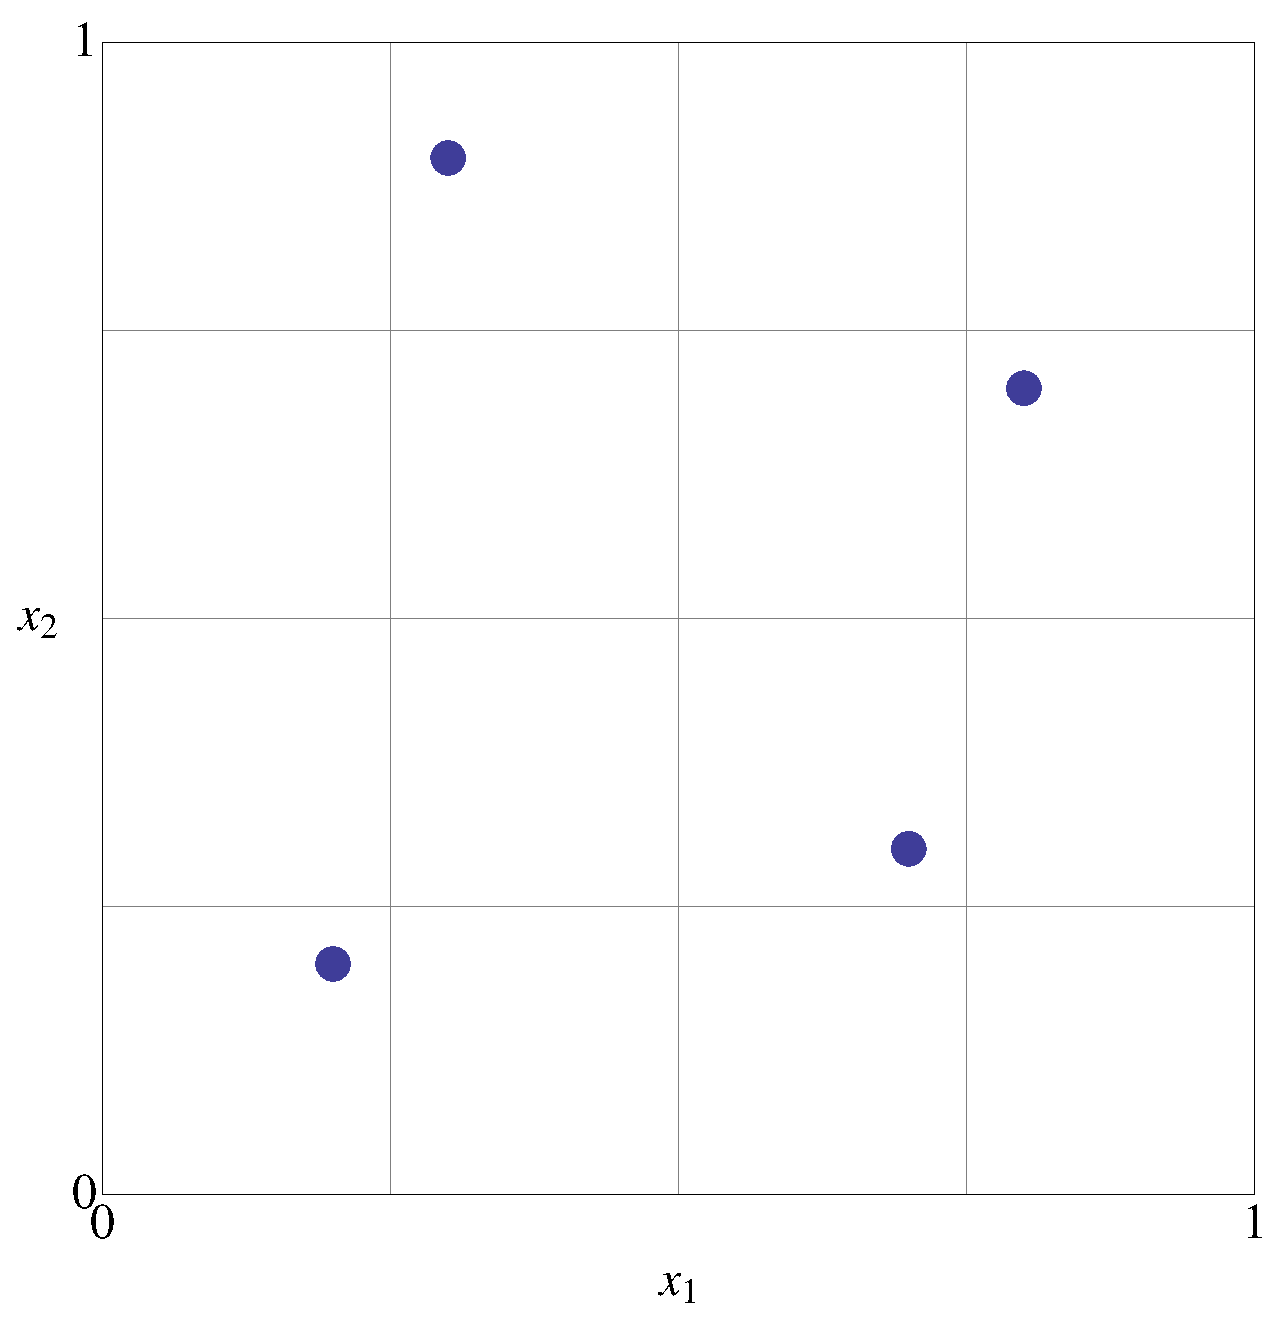
\includegraphics[scale=0.35]{images/lhs_graphic}
  \caption{An example of Latin hypercube sampling with four bins in
    design parameters $x_1$ and $x_2$. The dots
    are the sample sites.}
  \label{dace:figure01}
\end{figure}

The actual algorithm for generating Latin hypercube samples is more
complex than indicated by the description given above. For example,
the Latin hypercube sampling method implemented in the LHS
code~\cite{Swi04} takes into account a user-specified correlation
structure when selecting the sample sites. For more details on the
implementation of the LHS algorithm, see Reference~\cite{Swi04}.

\subsection{Uncertainty Quantification Example using Sampling Methods}\label{uq:uncertainty1}

The two-variable Textbook example problem (see
Equation~\ref{tutorial:textbook_f}) will be used to demonstrate
the application of sampling methods for uncertainty quantification
where it is assumed that $x_1$ and $x_2$ are uniform uncertain
variables on the interval $[0,1]$. The DAKOTA input file for this
problem is shown in Figure~\ref{uq:figure01}. The number of samples to
perform is controlled with the \texttt{samples} specification, the
type of sampling algorithm to use is controlled with the
\texttt{sample\_type} specification, the levels used for computing
statistics on the response functions is specified with the
\texttt{response\_levels} input, and the \texttt{seed} specification
controls the sequence of the pseudo-random numbers generated by the
sampling algorithms. The input samples generated are shown in
Figure~\ref{uq:figure02} for the case where \texttt{samples} = 5 and
\texttt{samples} = 10 for both \texttt{random} ($\circ$) and 
\texttt{lhs} ($+$) sample types.

\begin{figure}
  \centering \begin{bigbox} \begin{small}
  \verbatimtabinput[8]{dakota_uq_sampling.in} \end{small} \end{bigbox}
\caption{DAKOTA input file for UQ example using LHS sampling.}
\label{uq:figure01}
\end{figure}

\begin{figure}
  \centering
  \subfigure{\includegraphics[scale=0.35]{images/input_samples5}}
  \subfigure{\includegraphics[scale=0.35]{images/input_samples10}}
  \caption{Distribution of input sample points for random ($\triangle$)
    and lhs ($+$) sampling for \texttt{samples=5} and \texttt{10}.}
  \label{uq:figure02}
\end{figure}

Latin hypercube sampling ensures full coverage of the range of the
input variables, which is often a problem with Monte Carlo sampling
when the number of samples is small. In the case of \texttt{samples =
5}, poor stratification is evident in $x_1$ as four out of the five
Monte Carlo samples are clustered in the range $0.35 < x_1 < 0.55$,
and the regions $x_1 < 0.3$ and $0.6 < x_1 < 0.9$ are completely
missed. For the case where \texttt{samples = 10}, some clustering in
the Monte Carlo samples is again evident with \texttt{4} samples in
the range $0.5 < x_1 < 0.55$. In both cases, the stratification with
LHS is superior.  The response function statistics returned by DAKOTA
are shown in Figure~\ref{uq:figure03}.  The first two blocks of output
specify the response sample means and sample standard deviations and
confidence intervals for these statistics, as well as coefficients of
variation.  The last section of the output defines CDF pairs
(\texttt{distribution cumulative} was specified) for the response
functions by presenting the probability levels corresponding to the
specified response levels (\texttt{response\_levels} were set and the
default \texttt{compute probabilities} was used).  Alternatively,
DAKOTA could have provided CCDF pairings, reliability levels
corresponding to prescribed response levels, or response levels
corresponding to prescribed probability or reliability levels.

\begin{figure}
\centering
\begin{bigbox}
\begin{small}
\begin{verbatim}
Statistics based on 10 samples:

Moments for each response function:
response_fn_1:  Mean = 3.83840e-01  Std. Dev. = 4.02815e-01
                Coeff. of Variation = 1.04944e+00
response_fn_2:  Mean = 7.47987e-02  Std. Dev. = 3.46861e-01
                Coeff. of Variation = 4.63726e+00
response_fn_3:  Mean = 7.09462e-02  Std. Dev. = 3.41532e-01
                Coeff. of Variation = 4.81397e+00

95% confidence intervals for each response function:
response_fn_1:  Mean = (  9.56831e-02, 6.71997e-01 ),
             Std Dev = (  2.77071e-01, 7.35384e-01 )
response_fn_2:  Mean = ( -1.73331e-01, 3.22928e-01 ),
             Std Dev = (  2.38583e-01, 6.33233e-01 )
response_fn_3:  Mean = ( -1.73371e-01, 3.15264e-01 ),
             Std Dev = (  2.34918e-01, 6.23505e-01 )

Probabilities for each response function:
Cumulative Distribution Function (CDF) for response_fn_1:
     Response Level  Probability Level  Reliability Index
     --------------  -----------------  -----------------
   1.0000000000e-01   3.0000000000e-01
   2.0000000000e-01   5.0000000000e-01
   6.0000000000e-01   7.0000000000e-01
Cumulative Distribution Function (CDF) for response_fn_2:
     Response Level  Probability Level  Reliability Index
     --------------  -----------------  -----------------
   1.0000000000e-01   5.0000000000e-01
   2.0000000000e-01   7.0000000000e-01
   6.0000000000e-01   9.0000000000e-01
Cumulative Distribution Function (CDF) for response_fn_3:
     Response Level  Probability Level  Reliability Index
     --------------  -----------------  -----------------
   1.0000000000e-01   6.0000000000e-01
   2.0000000000e-01   6.0000000000e-01
   6.0000000000e-01   9.0000000000e-01
\end{verbatim}
\end{small}
\end{bigbox}
\caption{DAKOTA response function statistics from UQ sampling example.}
\label{uq:figure03}
\end{figure}

In addition to obtaining statistical summary information of the type
shown in Figure~\ref{uq:figure03}, the results of LHS sampling also
include correlations.  Four types of correlations are returned in the
output: simple and partial ``raw'' correlations, and simple and
partial ``rank'' correlations.  The raw correlations refer to
correlations performed on the actual input and output data.  Rank
correlations refer to correlations performed on the ranks of the data.
Ranks are obtained by replacing the actual data by the ranked values,
which are obtained by ordering the data in ascending order.  For
example, the smallest value in a set of input samples would be given a
rank 1, the next smallest value a rank 2, etc.  Rank correlations are
useful when some of the inputs and outputs differ greatly in
magnitude: then it is easier to compare if the smallest ranked input
sample is correlated with the smallest ranked output, for example.

Correlations are always calculated between two sets of sample data.
One can calculate correlation coefficients between two input
variables, between an input and an output variable (probably the most
useful), or between two output variables.  The simple correlation
coefficients presented in the output tables are Pearson's correlation
coefficient, which is defined for two variables $x$ and $y$ as:
$\mathtt{Corr}(x,y) = \frac{\sum_{i}(x_{i}-\bar{x})(y_{i}-\bar{y})}
{\sqrt{\sum_{i}(x_{i}-\bar{x})^2\sum_{i}(y_{i}-\bar{y})^2}}$.
Partial correlation coefficients are similar to simple correlations,
but a partial correlation coefficient between two variables measures
their correlation while adjusting for the effects of the other
variables.  For example, say one has a problem with two inputs and one
output; and the two inputs are highly correlated.  Then the
correlation of the second input and the output may be very low after
accounting for the effect of the first input.  The rank correlations
in DAKOTA are obtained using Spearman's rank correlation.  Spearman's
rank is the same as the Pearson correlation coefficient except that it
is calculated on the rank data.

Figure~\ref{uq:figure04} shows an example of the correlation output
provided by DAKOTA for the input file in Figure~\ref{uq:figure01}.
Note that these correlations are presently only available when one
specifies \texttt{lhs} as the sampling method under \texttt{sampling}.
Also note that the simple and partial correlations should be similar in most
cases (in terms of values of correlation coefficients).  This is
because we use a default ``restricted pairing'' method in the LHS
routine which forces near-zero correlation amongst uncorrelated
inputs.

\begin{figure}
\centering
\begin{bigbox}
\begin{small}
\begin{verbatim}
Simple Correlation Matrix between input and output:
                       x1           x2 response_fn_1 response_fn_2 response_fn_3
          x1  1.00000e+00
          x2 -7.22482e-02  1.00000e+00
response_fn_1 -7.04965e-01 -6.27351e-01  1.00000e+00
response_fn_2  8.61628e-01 -5.31298e-01 -2.60486e-01  1.00000e+00
response_fn_3 -5.83075e-01  8.33989e-01 -1.23374e-01 -8.92771e-01  1.00000e+00

Partial Correlation Matrix between input and output:
             response_fn_1 response_fn_2 response_fn_3
          x1 -9.65994e-01  9.74285e-01 -9.49997e-01
          x2 -9.58854e-01 -9.26578e-01  9.77252e-01

Simple Rank Correlation Matrix between input and output:
                       x1           x2 response_fn_1 response_fn_2 response_fn_3
          x1  1.00000e+00
          x2 -6.66667e-02  1.00000e+00
response_fn_1 -6.60606e-01 -5.27273e-01  1.00000e+00
response_fn_2  8.18182e-01 -6.00000e-01 -2.36364e-01  1.00000e+00
response_fn_3 -6.24242e-01  7.93939e-01 -5.45455e-02 -9.27273e-01  1.00000e+00

Partial Rank Correlation Matrix between input and output:
             response_fn_1 response_fn_2 response_fn_3
          x1 -8.20657e-01  9.74896e-01 -9.41760e-01
          x2 -7.62704e-01 -9.50799e-01  9.65145e-01
\end{verbatim}
\end{small}
\end{bigbox}
\caption{Correlation results using LHS Sampling.}
\label{uq:figure04}
\end{figure}

Finally, note that the LHS package can be used for design of
experiments over design and state variables by including the
\texttt{all\_variables} flag in the method specification section of
the DAKOTA input file. Then, instead of iterating on only the
uncertain variables, the LHS package will sample over all of the
variables.  In \texttt{all\_variables} mode, continuous design and
continuous state variables are treated as having uniform probability
distributions within their upper and lower bounds, discrete values are
sampled uniformly from within their sets or ranges, and any uncertain
variables are sampled within their specified probability distributions.

\subsection{Incremental Sampling}\label{uq:incremental}

In many situations, one may run an initial sample set and then need to
perform further sampling to get better estimates of the mean,
variance, and percentiles, and to obtain more comprehensive sample
coverage.  We call this capability incremental sampling. Currently,
the LHS incremental sampling capability we have in DAKOTA requires that
the incremental samples are double the sample size of the previous
sample.  That is, if one starts with a very small sample size of 10,
then one can use the incremental sampling capability to generate
sample sizes of 20, 40, 80, etc. Also, a DAKOTA restart file
(dakota.rst) must be available from the original sample. There are two
cases, random incremental and Latin Hypercube incremental sampling.
We assume that LHS incremental will be most frequently used.  One
major advantage of LHS incremental sampling is that it maintains the
stratification and correlation structure of the original LHS sample.
That is, if one generated 2 independent LHS samples and just merged
them, the calculation of the accuracy of statistical measures such as
the mean and the variance would be slightly incorrect.  However, in
the incremental case, the full sample (double the original size) is a
Latin Hypercube sample itself and statistical measures and their
accuracy can be properly calculated.  The incremental sampling
capability is most useful when one is starting off with very small
samples. Once the sample size is more than a few hundred, the benefit
of incremental sampling diminishes.

\begin{enumerate}

\item Incremental Random Sampling.  With incremental random sampling, 
the original sample set with N samples must be 
generated using \texttt{sample\_type} as \texttt{random}.
Then, the user can create a new DAKOTA input file that is very similar to the 
original one except the \texttt{sample\_type} should be defined to be 
\texttt{incremental\_random}.  Random incremental sampling does not 
require a doubling of samples each time.  Thus, the user 
can specify the number of samples (\texttt{samples}) to be a desired 
number (it can range from an additional one sample to a large integer), 
and the \texttt{previous\_samples} should be specified as N.  For example, if
the first sample has 50 samples, and 10 more samples are desired, 
in the second DAKOTA run, the number
of samples should be set to 60 and the number of previous samples set
to 50.  In this situation, only 10 new samples will be generated and
the final statistics will be reported on the full sample of 60. The
command line syntax for running the second sample is \texttt{dakota -i
input2.in -r dakota.rst} where input2.in is the input file with the
incremental sampling specification and dakota.rst is the restart file.
Note that if the restart file has a different name, that is fine; the
correct restart file name should be used.

\item Incremental Latin Hypercube Sampling. With incremental LHS sampling, 
the original sample set with N samples must be 
generated using \texttt{sample\_type} as \texttt{lhs}.
Then, the user can create a new DAKOTA input file that is very similar to the 
original one except the \texttt{sample\_type} should be defined to be 
\texttt{incremental\_lhs}, the number of samples (\texttt{samples}) should 
be 2N (twice the number of original samples), and
\texttt{previous\_samples} should be specified as N.  For example, if
the first sample has 50 samples, in the second DAKOTA run, the number
of samples should be set to 100 and the number of previous samples set
to 50.  In this situation, only 50 new samples will be generated and
the final statistics will be reported on the full sample of 100. The
command line syntax for running the second sample is \texttt{dakota -i
input2.in -r dakota.rst}, where input2.in is the input file with the
incremental sampling specification and dakota.rst is the restart file.
Note that if the restart file has a different name, that is fine; the
correct restart file name should be used.

\end{enumerate}

\section{Reliability Methods}\label{uq:reliability}

Reliability methods provide an alternative approach to uncertainty
quantification which can be less computationally demanding than
sampling techniques.  Reliability methods for uncertainty
quantification are based on probabilistic approaches that compute
approximate response function distribution statistics based on
specified uncertain variable distributions.  These response statistics
include response mean, response standard deviation, and cumulative or
complementary cumulative distribution functions (CDF/CCDF).  These
methods are often more efficient at computing statistics in the tails
of the response distributions (events with low probability) than
sampling based approaches since the number of samples required to
resolve a low probability can be prohibitive.

The methods all answer the fundamental question: ``Given a set of
uncertain input variables, $\mathbf{X}$, and a scalar response
function, $g$, what is the probability that the response function is
below or above a certain level, $\bar{z}$?'' The former can be written
as $P[g(\mathbf{X}) \le \bar{z}] = \mathit{F}_{g}(\bar{z})$ where
$\mathit{F}_{g}(\bar{z})$ is the cumulative distribution function
(CDF) of the uncertain response $g(\mathbf{X})$ over a set of response
levels.  The latter can be written as $P[g(\mathbf{X}) > \bar{z}]$ and
defines the complementary cumulative distribution function (CCDF).

This probability calculation involves a multi-dimensional integral
over an irregularly shaped domain of interest, $\mathbf{D}$, where
$g(\mathbf{X}) < z$ as displayed in Figure~\ref{uq:figure05} for the
case of two variables.  The reliability methods all involve the
transformation of the user-specified uncertain variables,
$\mathbf{X}$, with probability density function, $p(x_1,x_2)$, which
can be non-normal and correlated, to a space of independent Gaussian
random variables, $\mathbf{u}$, possessing a mean value of zero and
unit variance (i.e., standard normal variables). The region of
interest, $\mathbf{D}$, is also mapped to the transformed space to
yield, $\mathbf{D_{u}}$ , where $g(\mathbf{U}) < z$ as shown in
Figure~\ref{uq:figure06}.  The Nataf transformation~\cite{Der86},
which is identical to the Rosenblatt transformation~\cite{Ros52} in
the case of independent random variables, is used in DAKOTA to
accomplish this mapping. This transformation is performed to make the
probability calculation more tractable. In the transformed space,
probability contours are circular in nature as shown in
Figure~\ref{uq:figure06} unlike in the original uncertain variable
space, Figure~\ref{uq:figure05}. Also, the multi-dimensional integrals
can be approximated by simple functions of a single parameter,
$\beta$, called the reliability index.  $\beta$ is the minimum
Euclidean distance from the origin in the transformed space to the
response surface. This point is also known as the most probable point
(MPP) of failure. Note, however, the methodology is equally applicable
for generic functions, not simply those corresponding to failure
criteria; this nomenclature is due to the origin of these methods
within the disciplines of structural safety and reliability.
Note that there are local and global reliability methods.  The majority 
of the methods available are local, meaning that a local optimization 
formulation is used to locate one MPP.  In contrast, global methods
can find multiple MPPs if they exist.
\begin{figure}
  \centering
  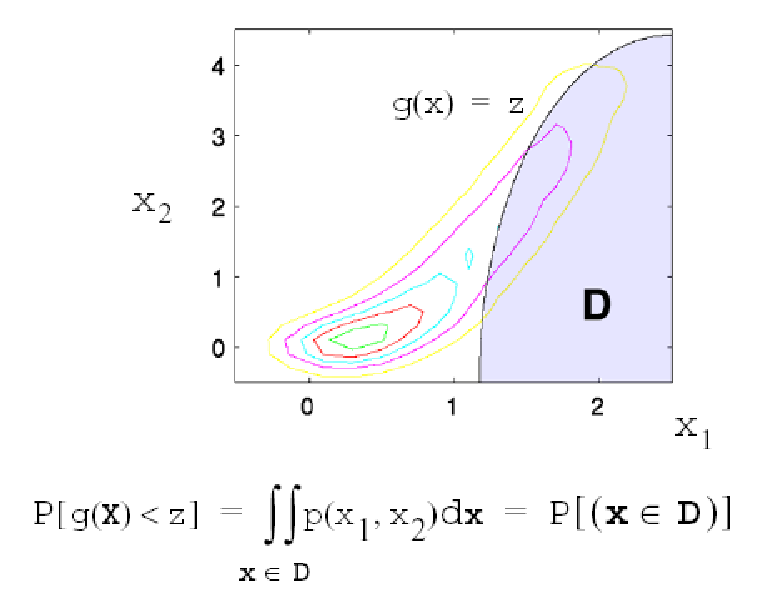
\includegraphics[scale=0.75]{images/cdf_orig_graphic}
  \caption{Graphical depiction of calculation of cumulative
    distribution function in the original uncertain variable space.}
  \label{uq:figure05}
\end{figure}

\begin{figure}
  \centering
  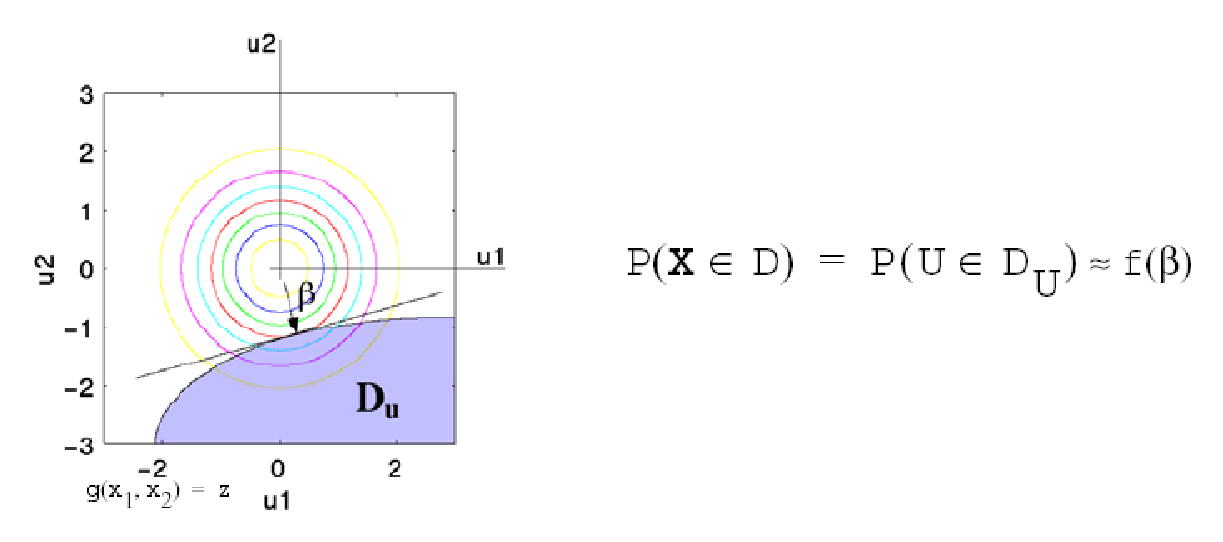
\includegraphics[scale=0.75]{images/cdf_tran_graphic}
  \caption{Graphical depiction of integration for the calculation of
    cumulative distribution function in the transformed uncertain
    variable space.}
  \label{uq:figure06}
\end{figure}

\subsection{Mean Value}\label{uq:reliability:mv}

The Mean Value method (MV, also known as MVFOSM in \cite{Hal00}) is
the simplest, least-expensive reliability method because it estimates
the response means, response standard deviations, and all CDF/CCDF
response-probability-reliability levels from a single evaluation of
response functions and their gradients at the uncertain variable
means.  This approximation can have acceptable accuracy when the
response functions are nearly linear and their distributions are
approximately Gaussian, but can have poor accuracy in other
situations.  The expressions for approximate response mean $\mu_g$,
approximate response variance $\sigma^2_g$, response target to
approximate probability/reliability level mapping ($\bar{z} \to p,\beta$),
and probability/reliability target to approximate response level mapping
($\bar{p},\bar{\beta} \to z$) are

\begin{eqnarray}
\mu_g      & = & g(\mu_{\bf x})  \label{eq:mv_mean1} \\
\sigma^2_g & = & \sum_i \sum_j Cov(i,j) \frac{dg}{dx_i}(\mu_{\bf x})
                 \frac{dg}{dx_j}(\mu_{\bf x}) \label{eq:mv_std_dev} \\
\beta_{cdf}  & = & \frac{\mu_g - \bar{z}}{\sigma_g} \label{eq:mv_ria_cdf} \\
\beta_{ccdf} & = & \frac{\bar{z} - \mu_g}{\sigma_g} \label{eq:mv_ria_ccdf} \\
z        & = & \mu_g - \sigma_g \bar{\beta}_{cdf} \label{eq:mv_pma_cdf} \\
z        & = & \mu_g + \sigma_g \bar{\beta}_{ccdf} \label{eq:mv_pma_ccdf}
\end{eqnarray}

respectively, where ${\bf x}$ are the uncertain values in the 
space of the original uncertain variables (``x-space''), $g({\bf x})$
is the limit state function (the response function for which
probability-response level pairs are needed), and $\beta_{cdf}$ and
$\beta_{ccdf}$ are the CDF and CCDF reliability indices, respectively.

With the introduction of second-order limit state information, MVSOSM
calculates a second-order mean as

\begin{equation}
\mu_g = g(\mu_{\bf x}) + \frac{1}{2} \sum_i \sum_j Cov(i,j) 
\frac{d^2g}{dx_i dx_j}(\mu_{\bf x}) \label{eq:mv_mean2}
\end{equation}

This is commonly combined with a first-order variance
(Equation~\ref{eq:mv_std_dev}), since second-order variance involves
higher order distribution moments (skewness, kurtosis)~\cite{Hal00}
which are often unavailable.

The first-order CDF probability $p(g \le z)$, first-order 
CCDF probability $p(g > z)$, $\beta_{cdf}$, and $\beta_{ccdf}$ are
related to one another through

\begin{eqnarray}
p(g \le z)   & = & \Phi(-\beta_{cdf})     \label{eq:p_cdf} \\
p(g > z)     & = & \Phi(-\beta_{ccdf})    \label{eq:p_ccdf} \\
\beta_{cdf}  & = & -\Phi^{-1}(p(g \le z)) \label{eq:beta_cdf} \\
\beta_{ccdf} & = & -\Phi^{-1}(p(g > z))   \label{eq:beta_ccdf} \\
\beta_{cdf}  & = & -\beta_{ccdf}          \label{eq:beta_cdf_ccdf} \\
p(g \le z)   & = & 1 - p(g > z)           \label{eq:p_cdf_ccdf}
\end{eqnarray}

where $\Phi()$ is the standard normal cumulative distribution
function.  A common convention in the literature is to define $g$ in
such a way that the CDF probability for a response level $z$ of zero
(i.e., $p(g \le 0)$) is the response metric of interest.  DAKOTA is
not restricted to this convention and is designed to support CDF or
CCDF mappings for general response, probability, and reliability level
sequences.

With the Mean Value method, it is possible to obtain 
importance factors indicating the relative importance of 
input variables.  The importance factors can be viewed
as an extension of linear sensitivity analysis combining deterministic
gradient information with input uncertainty information,
\emph{i.e}. input variable standard deviations. The accuracy of the
importance factors is contingent of the validity of the linear
approximation used to approximate the true response functions.
The importance factors are determined as: 

\begin{equation}
ImpFactor_i  = ({\frac{\sigma_{x_{i}}}{\sigma_g}}{\frac{dg}{dx_i}(\mu_{\bf x})})^2
\end{equation}


\subsection{MPP Search Methods}\label{uq:reliability:mpp}

All other local reliability methods solve an equality-constrained nonlinear
optimization problem to compute a most probable point (MPP) and then
integrate about this point to compute probabilities.  The MPP search
is performed in uncorrelated standard normal space (``u-space'') since
it simplifies the probability integration: the distance of the MPP
from the origin has the meaning of the number of input standard
deviations separating the mean response from a particular response
threshold.  The transformation from correlated non-normal
distributions (x-space) to uncorrelated standard normal distributions
(u-space) is denoted as ${\bf u} = T({\bf x})$ with the reverse
transformation denoted as ${\bf x} = T^{-1}({\bf u})$.  These
transformations are nonlinear in general, and possible approaches
include the Rosenblatt~\cite{Ros52}, Nataf~\cite{Der86}, and
Box-Cox~\cite{Box64} transformations.  The nonlinear transformations
may also be linearized, and common approaches for this include the
Rackwitz-Fiessler~\cite{Rac78} two-parameter equivalent normal and the
Chen-Lind~\cite{Che83} and Wu-Wirsching~\cite{Wu87} three-parameter
equivalent normals.  DAKOTA employs the Nataf nonlinear transformation
which is suitable for the common case when marginal distributions and
a correlation matrix are provided, but full joint distributions are
not known\footnote{If joint distributions are known, then the
Rosenblatt transformation is preferred.}.  This transformation occurs 
in the following two steps.  To transform between the
original correlated x-space variables and correlated standard normals
(``z-space''), a CDF matching condition is applied for each of the
marginal distributions:
\begin{equation}
\Phi(z_i) = F(x_i) \label{eq:trans_zx}
\end{equation}
where $F()$ is the cumulative distribution function of the original
probability distribution.  Then, to transform between correlated
z-space variables and uncorrelated u-space variables, the Cholesky 
factor ${\bf L}$ of a modified correlation matrix is used:
\begin{equation}
{\bf z} = {\bf L} {\bf u} \label{eq:trans_zu}
\end{equation}
where the original correlation matrix for non-normals in x-space has
been modified to represent the corresponding ``warped'' correlation in 
z-space~\cite{Der86}.

The forward reliability analysis algorithm of computing CDF/CCDF
probability/reliability levels for specified response levels is called
the reliability index approach (RIA), and the inverse reliability
analysis algorithm of computing response levels for specified CDF/CCDF
probability/reliability levels is called the performance measure
approach (PMA)~\cite{Tu99}.  The differences between the RIA and PMA
formulations appear in the objective function and equality constraint
formulations used in the MPP searches.  For RIA, the MPP search for
achieving the specified response level $\bar{z}$ is formulated as
computing the minimum distance in u-space from the origin to the
$\bar{z}$ contour of the limit state response function:
\begin{eqnarray}
{\rm minimize}     & {\bf u}^T {\bf u} \nonumber \\
{\rm subject \ to} & G({\bf u}) = \bar{z} \label{eq:ria_opt}
\end{eqnarray}

and for PMA, the MPP search for achieving the specified
reliability/probability level $\bar{\beta},\bar{p}$ is formulated as
computing the minimum/maximum response function value corresponding
to a prescribed distance from the origin in u-space:
\begin{eqnarray}
{\rm minimize}     & \pm G({\bf u}) \nonumber \\
{\rm subject \ to} & {\bf u}^T {\bf u} = \bar{\beta}^2 \label{eq:pma_opt}
\end{eqnarray}

where ${\bf u}$ is a vector centered at the origin in 
u-space and $g({\bf x}) \equiv G({\bf u})$ by definition.  In the RIA
case, the optimal MPP solution ${\bf u}^*$ defines the reliability 
index from $\beta = \pm \|{\bf u}^*\|_2$, which in turn defines the 
CDF/CCDF probabilities (using Equations~\ref{eq:p_cdf}-\ref{eq:p_ccdf} in 
the case of first-order integration).  The sign of $\beta$ is defined by
\begin{eqnarray}
G({\bf u}^*) > G({\bf 0}): \beta_{cdf} < 0, \beta_{ccdf} > 0 \\
G({\bf u}^*) < G({\bf 0}): \beta_{cdf} > 0, \beta_{ccdf} < 0
\end{eqnarray}
\noindent where $G({\bf 0})$ is the median limit state response computed 
at the origin in u-space\footnote{It is not necessary to explicitly compute
the median response since the sign of the inner product 
$\langle {\bf u}^*, \nabla_{\bf u} G \rangle$
can be used to determine the orientation of the optimal response with 
respect to the median response.} (where $\beta_{cdf}$ = $\beta_{ccdf}$ = 0 
and first-order $p(g \le z)$ = $p(g > z)$ = 0.5).  In the PMA case, the 
sign applied to $G({\bf u})$ (equivalent to minimizing or maximizing 
$G({\bf u})$) is similarly defined by $\bar{\beta}$
\begin{eqnarray}
\bar{\beta}_{cdf} < 0, \bar{\beta}_{ccdf} > 0: {\rm maximize \ } G({\bf u}) \\
\bar{\beta}_{cdf} > 0, \bar{\beta}_{ccdf} < 0: {\rm minimize \ } G({\bf u})
\end{eqnarray}
and the limit state at the MPP ($G({\bf u}^*)$) defines the desired
response level result.

\subsubsection{Limit state approximations} \label{uq:reliability:mpp:approx}

There are a variety of algorithmic variations that are available for
use within RIA/PMA reliability analyses.  First, one may select among
several different limit state approximations that can be used to
reduce computational expense during the MPP searches.  Local,
multipoint, and global approximations of the limit state are possible.
\cite{Eld05} investigated local first-order limit state 
approximations, and \cite{Eld06a} investigated local second-order
and multipoint approximations.  These techniques include:

\begin{enumerate}
\item a single Taylor series per response/reliability/probability level 
in x-space centered at the uncertain variable means.  The first-order 
approach is commonly known as the Advanced Mean Value (AMV) method:
\begin{equation}
g({\bf x}) \cong g(\mu_{\bf x}) + \nabla_x g(\mu_{\bf x})^T 
({\bf x} - \mu_{\bf x}) \label{eq:linear_x_mean}
\end{equation}
and the second-order approach has been named AMV$^2$:
\begin{equation}
g({\bf x}) \cong g(\mu_{\bf x}) + \nabla_{\bf x} g(\mu_{\bf x})^T 
({\bf x} - \mu_{\bf x}) + \frac{1}{2} ({\bf x} - \mu_{\bf x})^T 
\nabla^2_{\bf x} g(\mu_{\bf x}) ({\bf x} - \mu_{\bf x})
\label{eq:taylor2_x_mean}
\end{equation}

\item same as AMV/AMV$^2$, except that the Taylor series is expanded 
in u-space.  The first-order option has been termed the u-space AMV 
method:
\begin{equation}
G({\bf u}) \cong G(\mu_{\bf u}) + \nabla_u G(\mu_{\bf u})^T 
({\bf u} - \mu_{\bf u}) \label{eq:linear_u_mean}
\end{equation}
where $\mu_{\bf u} = T(\mu_{\bf x})$ and is nonzero in general, and 
the second-order option has been named the u-space AMV$^2$ method:
\begin{equation}
G({\bf u}) \cong G(\mu_{\bf u}) + \nabla_{\bf u} G(\mu_{\bf u})^T 
({\bf u} - \mu_{\bf u}) + \frac{1}{2} ({\bf u} - \mu_{\bf u})^T 
\nabla^2_{\bf u} G(\mu_{\bf u}) ({\bf u} - \mu_{\bf u}) 
\label{eq:taylor2_u_mean}
\end{equation}

\item an initial Taylor series approximation in x-space at the uncertain 
variable means, with iterative expansion updates at each MPP estimate
(${\bf x}^*$) until the MPP converges.  The first-order option is
commonly known as AMV+:
\begin{equation}
g({\bf x}) \cong g({\bf x}^*) + \nabla_x g({\bf x}^*)^T ({\bf x} - {\bf x}^*)
\label{eq:linear_x_mpp}
\end{equation}
and the second-order option has been named AMV$^2$+:
\begin{equation}
g({\bf x}) \cong g({\bf x}^*) + \nabla_{\bf x} g({\bf x}^*)^T 
({\bf x} - {\bf x}^*) + \frac{1}{2} ({\bf x} - {\bf x}^*)^T 
\nabla^2_{\bf x} g({\bf x}^*) ({\bf x} - {\bf x}^*) \label{eq:taylor2_x_mpp}
\end{equation}

\item same as AMV+/AMV$^2$+, except that the expansions are performed in 
u-space.  The first-order option has been termed the u-space AMV+ method.
\begin{equation}
G({\bf u}) \cong G({\bf u}^*) + \nabla_u G({\bf u}^*)^T ({\bf u} - {\bf u}^*)
\label{eq:linear_u_mpp}
\end{equation}
and the second-order option has been named the u-space AMV$^2$+ method:
\begin{equation}
G({\bf u}) \cong G({\bf u}^*) + \nabla_{\bf u} G({\bf u}^*)^T 
({\bf u} - {\bf u}^*) + \frac{1}{2} ({\bf u} - {\bf u}^*)^T 
\nabla^2_{\bf u} G({\bf u}^*) ({\bf u} - {\bf u}^*) \label{eq:taylor2_u_mpp}
\end{equation}

\item a multipoint approximation in x-space. This approach involves a 
Taylor series approximation in intermediate variables where the powers
used for the intermediate variables are selected to match information at
the current and previous expansion points.  Based on the 
two-point exponential approximation concept (TPEA, \cite{Fad90}), the 
two-point adaptive nonlinearity approximation (TANA-3, \cite{Xu98})
approximates the limit state as:
\begin{equation}
g({\bf x}) \cong g({\bf x}_2) + \sum_{i=1}^n 
\frac{\partial g}{\partial x_i}({\bf x}_2) \frac{x_{i,2}^{1-p_i}}{p_i} 
(x_i^{p_i} - x_{i,2}^{p_i}) + \frac{1}{2} \epsilon({\bf x}) \sum_{i=1}^n 
(x_i^{p_i} - x_{i,2}^{p_i})^2 \label{eq:tana_g}
\end{equation}

\noindent where $n$ is the number of uncertain variables and:
\begin{eqnarray}
p_i & = & 1 + \ln \left[ \frac{\frac{\partial g}{\partial x_i}({\bf x}_1)}
{\frac{\partial g}{\partial x_i}({\bf x}_2)} \right] \left/ 
\ln \left[ \frac{x_{i,1}}{x_{i,2}} \right] \right. \label{eq:tana_pi_x} \\
\epsilon({\bf x}) & = & \frac{H}{\sum_{i=1}^n (x_i^{p_i} - x_{i,1}^{p_i})^2 + 
\sum_{i=1}^n (x_i^{p_i} - x_{i,2}^{p_i})^2} \label{eq:tana_eps_x} \\
H & = & 2 \left[ g({\bf x}_1) - g({\bf x}_2) - \sum_{i=1}^n 
\frac{\partial g}{\partial x_i}({\bf x}_2) \frac{x_{i,2}^{1-p_i}}{p_i} 
(x_{i,1}^{p_i} - x_{i,2}^{p_i}) \right] \label{eq:tana_H_x}
\end{eqnarray}
\noindent and ${\bf x}_2$ and ${\bf x}_1$ are the current and previous
MPP estimates in x-space, respectively.  Prior to the availability of
two MPP estimates, x-space AMV+ is used.

\item a multipoint approximation in u-space. The u-space TANA-3
approximates the limit state as:
\begin{equation}
G({\bf u}) \cong G({\bf u}_2) + \sum_{i=1}^n 
\frac{\partial G}{\partial u_i}({\bf u}_2) \frac{u_{i,2}^{1-p_i}}{p_i} 
(u_i^{p_i} - u_{i,2}^{p_i}) + \frac{1}{2} \epsilon({\bf u}) \sum_{i=1}^n 
(u_i^{p_i} - u_{i,2}^{p_i})^2 \label{eq:tana_G}
\end{equation}

\noindent where:
\begin{eqnarray}
p_i & = & 1 + \ln \left[ \frac{\frac{\partial G}{\partial u_i}({\bf u}_1)}
{\frac{\partial G}{\partial u_i}({\bf u}_2)} \right] \left/ 
\ln \left[ \frac{u_{i,1}}{u_{i,2}} \right] \right. \label{eq:tana_pi_u} \\
\epsilon({\bf u}) & = & \frac{H}{\sum_{i=1}^n (u_i^{p_i} - u_{i,1}^{p_i})^2 + 
\sum_{i=1}^n (u_i^{p_i} - u_{i,2}^{p_i})^2} \label{eq:tana_eps_u} \\
H & = & 2 \left[ G({\bf u}_1) - G({\bf u}_2) - \sum_{i=1}^n 
\frac{\partial G}{\partial u_i}({\bf u}_2) \frac{u_{i,2}^{1-p_i}}{p_i} 
(u_{i,1}^{p_i} - u_{i,2}^{p_i}) \right] \label{eq:tana_H_u}
\end{eqnarray}
\noindent and ${\bf u}_2$ and ${\bf u}_1$ are the current and previous
MPP estimates in u-space, respectively.  Prior to the availability of
two MPP estimates, u-space AMV+ is used.

\item the MPP search on the original response functions without the 
use of any approximations.  Combining this option with first-order and
second-order integration approaches (see next section) results in the
traditional first-order and second-order reliability methods (FORM and
SORM).
\end{enumerate}

The Hessian matrices in AMV$^2$ and AMV$^2$+ may be available
analytically, estimated numerically, or approximated through
quasi-Newton updates.  The selection between x-space or u-space for
performing approximations depends on where the approximation will be
more accurate, since this will result in more accurate MPP estimates
(AMV, AMV$^2$) or faster convergence (AMV+, AMV$^2$+, TANA).  Since
this relative accuracy depends on the forms of the limit state $g(x)$
and the transformation $T(x)$ and is therefore application dependent
in general, DAKOTA supports both options.  A concern with
approximation-based iterative search methods (i.e., AMV+, AMV$^2$+ and
TANA) is the robustness of their convergence to the MPP.  It is
possible for the MPP iterates to oscillate or even diverge.  However,
to date, this occurrence has been relatively rare, and DAKOTA contains
checks that monitor for this behavior.  Another concern with TANA is
numerical safeguarding (e.g., the possibility of raising negative
$x_i$ or $u_i$ values to nonintegral $p_i$ exponents in
Equations~\ref{eq:tana_g}, \ref{eq:tana_eps_x}-\ref{eq:tana_G},
and~\ref{eq:tana_eps_u}-\ref{eq:tana_H_u}).  Safeguarding involves
offseting negative $x_i$ or $u_i$ and, for potential numerical
difficulties with the logarithm ratios in Equations~\ref{eq:tana_pi_x}
and~\ref{eq:tana_pi_u}, reverting to either the linear ($p_i = 1$) or
reciprocal ($p_i = -1$) approximation based on which approximation has
lower error in $\frac{\partial g}{\partial x_i}({\bf x}_1)$ or
$\frac{\partial G}{\partial u_i}({\bf u}_1)$.

\subsubsection{Probability integrations} \label{uq:reliability:mpp:int}

The second algorithmic variation involves the integration approach for
computing probabilities at the MPP, which can be selected to be
first-order (Equations~\ref{eq:p_cdf}-\ref{eq:p_ccdf}) or second-order
integration.  Second-order integration involves applying a curvature
correction~\cite{Bre84,Hoh88,Hon99}.  Breitung applies a correction
based on asymptotic analysis~\cite{Bre84}:
\begin{equation}
p = \Phi(-\beta_p) \prod_{i=1}^{n-1} \frac{1}{\sqrt{1 + \beta_p \kappa_i}}
\label{eq:p_2nd_breit}
\end{equation}
where $\kappa_i$ are the principal curvatures of the limit state
function (the eigenvalues of an orthonormal transformation of
$\nabla^2_{\bf u} G$, taken positive for a convex limit state) and
$\beta_p \ge 0$ (a CDF or CCDF probability correction is selected to
obtain the correct sign for $\beta_p$).  An alternate correction in
\cite{Hoh88} is consistent in the asymptotic regime ($\beta_p \to \infty$) 
but does not collapse to first-order integration for $\beta_p = 0$:
\begin{equation}
p = \Phi(-\beta_p) \prod_{i=1}^{n-1} 
\frac{1}{\sqrt{1 + \psi(-\beta_p) \kappa_i}} \label{eq:p_2nd_hr}
\end{equation}
where $\psi() = \frac{\phi()}{\Phi()}$ and $\phi()$ is the standard
normal density function.  \cite{Hon99} applies further corrections to
Equation~\ref{eq:p_2nd_hr} based on point concentration methods.  At
this time, all three approaches are available within the code, but the
Hohenbichler-Rackwitz correction is used by default (switching the 
correction is a compile-time option in the source code and has not
not currently been exposed in the input specification).

\subsubsection{Method mapping} \label{uq:reliability:mpp:map}

Given settings for limit state approximation, approximation order,
integration approach, and other details presented to this point, it is
evident that the number of algorithmic combinations is high.
Table~\ref{tab:rel_meth_map} provides a succinct mapping for some of
these combinations to common method names from the reliability
literature, where blue indicates the most well-known combinations and
gray indicates other supported combinations.
\begin{table}
\centering
\caption{Mapping from DAKOTA options to standard reliability methods.}
\label{tab:rel_meth_map}
\begin{tabular}{|c|c|c|}
\hline
& \multicolumn{2}{c|}{Order of approximation and integration} \\ \cline{2-3}
MPP search      & First order & Second order                        \\ \hline
none            & \cellcolor{blue}\textcolor{white}{MVFOSM}
                & \cellcolor[gray]{0.5}\textcolor{black}{MVSOSM}   \\ \hline
x\_taylor\_mean & \cellcolor{blue}\textcolor{white}{AMV}
                & \cellcolor[gray]{0.5}\textcolor{black}{AMV$^2$}  \\ \hline
u\_taylor\_mean & \cellcolor[gray]{0.5}\textcolor{black}{u-space AMV}
                & \cellcolor[gray]{0.5}\textcolor{black}{u-space AMV$^2$} \\
\hline
x\_taylor\_mpp  & \cellcolor{blue}\textcolor{white}{AMV+}
                & \cellcolor[gray]{0.5}\textcolor{black}{AMV$^2$+} \\ \hline
u\_taylor\_mpp  & \cellcolor[gray]{0.5}\textcolor{black}{u-space AMV+}
                & \cellcolor[gray]{0.5}\textcolor{black}{u-space AMV$^2$+} \\
\hline
x\_two\_point   & \cellcolor{blue}\textcolor{white}{TANA}
                & \cellcolor[gray]{0.5}                             \\ \hline
u\_two\_point   & \cellcolor[gray]{0.5}\textcolor{black}{u-space TANA}
                & \cellcolor[gray]{0.5}                             \\ \hline
no\_approx      & \cellcolor{blue}\textcolor{white}{FORM}
                & \cellcolor{blue}\textcolor{white}{SORM}           \\ \hline
\end{tabular}
\end{table}

Within the DAKOTA specification (refer to the Method Commands chapter
within the Reference Manual), the MPP search and integration order
selections are explicit in the method specification, but the order of
the approximation is inferred from the associated response
specification (as is done with local taylor series approximations
described in Section~\ref{models:surf:taylor}).  Thus, reliability
methods do not have to be synchronized in order as shown in the table;
however, it is often desirable to do so.


\subsection{Global Reliability Methods}\label{uq:reliability:global}

Global reliability methods are designed to handle nonsmooth and
multimodal failure surfaces, by creating global approximations based
on Gaussian process models. They accurately resolve a particular
contour of a response function and then estimate probabilities using
multimodal adaptive importance sampling.

The global reliability method in DAKOTA is called 
Efficient Global Reliability Analysis (EGRA) ~\cite{Bic07}.  
The name is due to its 
roots in efficient global optimization (EGO) ~\cite{Jon98,Hua06}.
The main idea in EGO-type optimization methods is that a global 
approximation is made of the underlying function.  This approximation, 
which is a Gaussian process model, is used to guide the search by finding 
points which maximize the expected improvement function (EIF). 
The EIF is used to select the location at which a new training point should be
added to the Gaussian process model by maximizing the amount of improvement 
in the objective function that can be expected by adding that point.
A point could be expected to produce an improvement in the objective function 
if its predicted value is better than the current best solution, or if the 
uncertainty in its prediction is such that the probability of it producing
a better solution is high.
Because the uncertainty is higher in regions of the design space with fewer
observations, this provides a balance between exploiting areas of the
design space that predict good solutions, and exploring areas where more
information is needed.

The general procedure of these EGO-type methods is:
\begin{enumerate}
\item Build an initial Gaussian process model of the objective function.
%\item Use cross validation to ensure that the GP model is satisfactory.
\item Find the point that maximizes the EIF.
      If the EIF value at this point is sufficiently small, stop.
\item Evaluate the objective function at the point where the EIF is maximized.
      Update the Gaussian process model using this new point.
      Go to Step 2.
\end{enumerate}

Gaussian process (GP) models are used because
they provide not just a predicted value at an unsampled point, but also an
estimate of the prediction variance.
This variance gives an indication of the uncertainty in the GP model, which
results from the construction of the covariance function.
This function is based on the idea that when input points are near one another,
the correlation between their corresponding outputs will be high.
As a result, the uncertainty associated with the model's predictions will be
small for input points which are near the points used to train the model,
and will increase as one moves further from the training points.

The expected improvement function is used in EGO algorithms 
to select the location at which a new training point should be added.
The EIF is defined as the expectation that any point in the search
space will provide a better solution than the current best solution
based on the expected values and variances predicted by the GP model.
It is important to understand how the use of this EIF leads to optimal
solutions.  The EIF indicates how much the objective function value at 
a new potential location 
is expected to be less than the predicted value at the current best solution.
Because the GP model provides a Gaussian distribution at each predicted
point, expectations can be calculated.
Points with good expected values and even a small variance will
have a significant expectation of producing a better solution (exploitation),
but so will points that have relatively poor expected values and greater
variance (exploration).
 
The application of EGO to reliability analysis, however, is made more
complicated due to the inclusion of equality constraints.
In forward reliability analysis, the response function appears as a 
constraint rather than the objective.  That is, we want to satisfy 
the constraint that the response equals a threshold value 
and is on the limit state:  $G({\bf u})\!=\!\bar{z}$.
Therefore, the EIF function was modified to focus on feasibility, 
and instead of using an expected improvement function, we use an 
expected feasibility function (EFF) ~\cite{Bic07}. 
The EFF provides an indication of how well the response is expected 
to satisfy the equality constraint.  
Points where the expected value is close to the threshold
($\mu_G\!\approx\!\bar{z}$) and points with a large uncertainty in the
prediction will have large expected feasibility values.

The general outline of the EGRA algorithm is as follows:  LHS sampling 
is used to generate a small number of samples from the true response 
function.  Then, an initial Gaussian process model is constructed. 
Based on the EFF, the point with maximum EFF is found using 
the global optimizer DIRECT.  The true response function is then 
evaluated at this new point, and this point is added to the sample set 
and the process of building a new GP model and maximizing the EFF is 
repeated until the maximum EFF is small.  At this stage, the GP model 
is accurate in the vicinity of the limit state.  The GP model 
is then used to calculate the probability of failure 
using multimodal importance sampling, which is explained below. 

One method to calculate the probability of failure is 
to directly perform the probability 
integration numerically by sampling the response function.
Sampling methods can be 
prohibitively expensive because they generally require a large 
number of response function evaluations.
Importance sampling methods reduce this expense by focusing the samples in 
the important regions of the uncertain space.
They do this by centering the sampling density function at the MPP rather
than at the mean.
This ensures the samples will lie the region of interest, 
thus increasing the efficiency of the sampling method.
Adaptive importance sampling (AIS) further improves the efficiency by 
adaptively updating the sampling density function.
Multimodal adaptive importance sampling~\cite{Dey98} is a 
variation of AIS that allows for the use of multiple sampling densities 
making it better suited for cases where multiple sections of the limit state 
are highly probable.

Note that importance sampling methods require that the location of at least 
one MPP be known because it is used to center the initial sampling density.
However, current gradient-based, local search methods used in MPP search may 
fail to converge or may converge to poor solutions for 
highly nonlinear problems, possibly making these methods inapplicable.
The EGRA algorithm described above does 
not depend on the availability of accurate gradient information, making
convergence more reliable for nonsmooth response functions.
Moreover, EGRA has the ability to locate multiple failure points, which 
can provide multiple starting points and thus a good multimodal sampling density for the initial steps of multimodal AIS.  The probability assessment 
using multimodal AIS thus incorporates probability of failure at 
multiple points.

\subsection{Uncertainty Quantification Example using Reliability Analysis} \label{uq:reliability:ex}

In summary, the user can choose to perform either forward (RIA) or
inverse (PMA) mappings when performing a reliability analysis.  With
either approach, there are a variety of methods from which to choose
in terms of limit state approximations (MVFOSM, MVSOSM, x-/u-space
AMV, x-/u-space AMV$^2$, x-/u-space AMV+, x-/u-space AMV$^2$+,
x-/u-space TANA, and FORM/SORM), probability integrations
(first-order or second-order), limit state Hessian selection
(analytic, finite difference, BFGS, or SR1), and MPP optimization
algorithm (SQP or NIP) selections.

All reliability methods output approximate values of the CDF/CCDF
response-probability-reliability levels for prescribed response levels
(RIA) or prescribed probability or reliability levels (PMA).  In
addition, the MV methods additionally output estimates of the mean and
standard deviation of the response functions along with importance
factors for each of the uncertain variables in the case of independent
random variables.

This example quantifies the uncertainty in the ``log ratio'' response
function:
\begin{equation}
g(x_1,x_2) = \frac{x_1}{x_2}
\end{equation}
by computing approximate response statistics using reliability
analysis to determine the response cumulative distribution function:
\begin{equation}
P[g(x_1,x_2) < \bar{z}]
\end{equation}
where $X_1$ and $X_2$ are identically distributed lognormal random
variables with means of \texttt{1}, standard deviations of
\texttt{0.5}, and correlation coefficient of \texttt{0.3}.

A DAKOTA input file showing RIA using FORM (option 7 in limit state
approximations combined with first-order integration) is listed in
Figure~\ref{uq:rel_input_form}.  The user first specifies the 
\texttt{local\_reliability} method, followed by the MPP search 
approach and integration order.  In this example, we specify
\texttt{mpp\_search no\_approx} and utilize the default first-order
integration to select FORM.  Finally, the user specifies response
levels or probability/reliability levels to determine if the problem
will be solved using an RIA approach or a PMA approach.  In the
example figure of~\ref{uq:rel_input_form}, we use RIA by specifying a range
of \texttt{response\_levels} for the problem.  The resulting output
for this input is shown in Figure~\ref{uq:rel_output_form}, with probability
and reliability levels listed for each response level.
Figure~\ref{uq:rel_form_compare} shows that FORM compares favorably to an
exact analytic solution for this problem.  Also note that FORM does have 
some error in the calculation of CDF values for this problem, but it is 
a very small error (on the order of e-11), much smaller than the 
error obtained when using a Mean Value method, which will be discussed next.


\begin{figure}
  \centering
  \begin{bigbox}
    \begin{small}
      \verbatimtabinput[8]{dakota_uq_reliability.in}
    \end{small}
  \end{bigbox}
\caption{DAKOTA input file for Reliability UQ example using FORM.}
\label{uq:rel_input_form}
\end{figure}

\begin{figure}
\centering
\begin{bigbox}
\begin{small}
\begin{verbatim}
Cumulative Distribution Function (CDF) for response_fn_1:
     Response Level  Probability Level  Reliability Index
     --------------  -----------------  -----------------
   4.0000000000e-01   4.7624085962e-02   1.6683404020e+00
   5.0000000000e-01   1.0346525475e-01   1.2620507942e+00
   5.5000000000e-01   1.3818404972e-01   1.0885143628e+00
   6.0000000000e-01   1.7616275822e-01   9.3008801339e-01
   6.5000000000e-01   2.1641741368e-01   7.8434989943e-01
   7.0000000000e-01   2.5803428381e-01   6.4941748143e-01
   7.5000000000e-01   3.0020938124e-01   5.2379840558e-01
   8.0000000000e-01   3.4226491013e-01   4.0628960782e-01
   8.5000000000e-01   3.8365052982e-01   2.9590705956e-01
   9.0000000000e-01   4.2393548232e-01   1.9183562480e-01
   1.0000000000e+00   5.0000000000e-01   6.8682233460e-12
   1.0500000000e+00   5.3539344228e-01  -8.8834907167e-02
   1.1500000000e+00   6.0043460094e-01  -2.5447217462e-01
   1.2000000000e+00   6.3004131827e-01  -3.3196278078e-01
   1.2500000000e+00   6.5773508987e-01  -4.0628960782e-01
   1.3000000000e+00   6.8356844630e-01  -4.7770089473e-01
   1.3500000000e+00   7.0761025532e-01  -5.4641676380e-01
   1.4000000000e+00   7.2994058691e-01  -6.1263331274e-01
   1.5000000000e+00   7.6981945355e-01  -7.3825238860e-01
   1.5500000000e+00   7.8755158269e-01  -7.9795460350e-01
   1.6000000000e+00   8.0393505584e-01  -8.5576118635e-01
   1.6500000000e+00   8.1906005158e-01  -9.1178881995e-01
   1.7000000000e+00   8.3301386860e-01  -9.6614373461e-01
   1.7500000000e+00   8.4588021938e-01  -1.0189229206e+00
\end{verbatim}
\end{small}
\end{bigbox}
\caption{Output from Reliability UQ example using FORM.}
\label{uq:rel_output_form}
\end{figure}

\begin{figure}
  \centering
  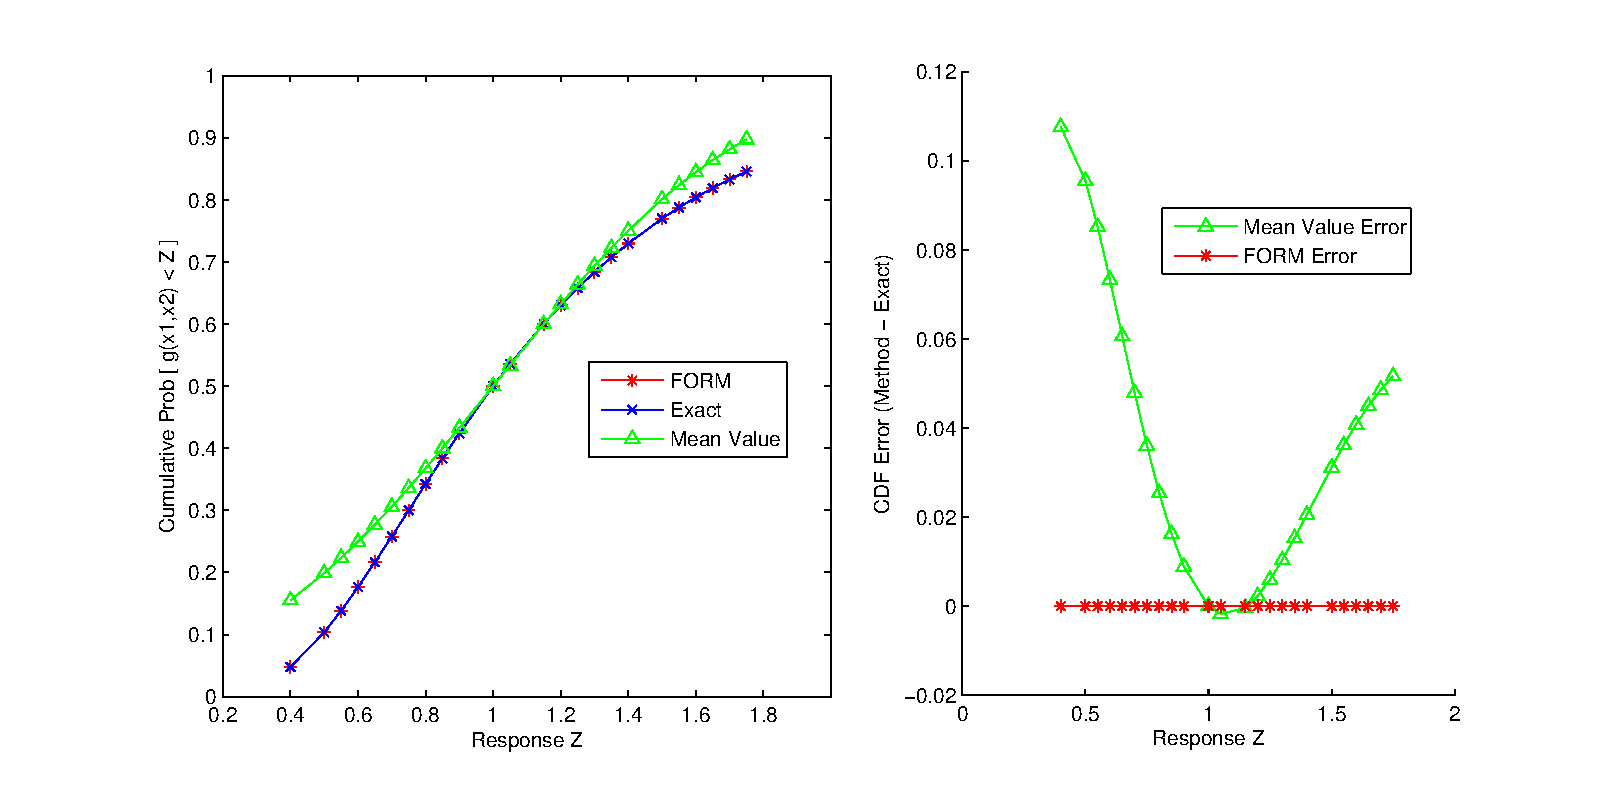
\includegraphics[scale=0.5]{images/cdf_form}
\caption{Comparison of the cumulative distribution function (CDF) computed by
FORM, the Mean Value method, and the exact CDF for $g(x_1,x_2)=\frac{x_1}{x_2}$}
\label{uq:rel_form_compare}
\end{figure}

If the user specifies \texttt{local\_reliability} as a method 
with no additional specification on how to do the MPP search, then no 
MPP search is done: the Mean Value method is used.  The MV results are
shown in Figure~\ref{uq:rel_output_mv} and consist of approximate mean
and standard deviation of the response, the importance factors for
each uncertain variable, and approximate probability/reliability
levels for the prescribed response levels that have been inferred from
the approximate mean and standard deviation (using
Equations~\ref{eq:mv_ria_cdf} and~\ref{eq:p_cdf}). It is evident that
the statistics are considerably different from the fully converged
FORM results; however, these rough approximations are also much less
expensive to calculate. The importance factors are a measure of the
sensitivity of the response function(s) to the uncertain input
variables, but in this case, are not separable due to the presence of
input correlation coefficients. A comparison of the mean value results 
with the FORM results is shown in Figure~\ref{uq:rel_form_compare}. 
The mean value results are not accurate near the tail values of the CDF, 
and can differ from the exact solution by as much as 0.11 in CDF estimates.
A comprehensive comparison of
various reliability methods applied to the logratio problem 
is provided in ~\cite{Eld06a}.

\begin{figure} % Imp factors only if uncorrelated
\begin{bigbox}
\begin{small}
\begin{verbatim}
MV Statistics for response_fn_1:
  Approximate Mean Response                  =  1.0000000000e+00
  Approximate Standard Deviation of Response =  5.9160798127e-01
  Importance Factors not available.
Cumulative Distribution Function (CDF) for response_fn_1:
     Response Level  Probability Level  Reliability Index
     --------------  -----------------  -----------------
   4.0000000000e-01   1.5524721837e-01   1.0141851006e+00
   5.0000000000e-01   1.9901236093e-01   8.4515425050e-01
   5.5000000000e-01   2.2343641149e-01   7.6063882545e-01
   6.0000000000e-01   2.4948115037e-01   6.7612340040e-01
   6.5000000000e-01   2.7705656603e-01   5.9160797535e-01
   7.0000000000e-01   3.0604494093e-01   5.0709255030e-01
   7.5000000000e-01   3.3630190949e-01   4.2257712525e-01
   8.0000000000e-01   3.6765834596e-01   3.3806170020e-01
   8.5000000000e-01   3.9992305332e-01   2.5354627515e-01
   9.0000000000e-01   4.3288618783e-01   1.6903085010e-01
   1.0000000000e+00   5.0000000000e-01   0.0000000000e+00
   1.0500000000e+00   5.3367668035e-01  -8.4515425050e-02
   1.1500000000e+00   6.0007694668e-01  -2.5354627515e-01
   1.2000000000e+00   6.3234165404e-01  -3.3806170020e-01
   1.2500000000e+00   6.6369809051e-01  -4.2257712525e-01
   1.3000000000e+00   6.9395505907e-01  -5.0709255030e-01
   1.3500000000e+00   7.2294343397e-01  -5.9160797535e-01
   1.4000000000e+00   7.5051884963e-01  -6.7612340040e-01
   1.5000000000e+00   8.0098763907e-01  -8.4515425050e-01
   1.5500000000e+00   8.2372893005e-01  -9.2966967555e-01
   1.6000000000e+00   8.4475278163e-01  -1.0141851006e+00
   1.6500000000e+00   8.6405064339e-01  -1.0987005257e+00
   1.7000000000e+00   8.8163821351e-01  -1.1832159507e+00
   1.7500000000e+00   8.9755305196e-01  -1.2677313758e+00
\end{verbatim}
\end{small}
\end{bigbox}
\caption{Output from Reliability UQ example using MV.}
\label{uq:rel_output_mv}
\end{figure}

Additional reliability analysis and design results are provided in 
Sections~\ref{additional:logratio}-\ref{additional:steel_column}.


\section{Stochastic Expansion Methods}\label{uq:expansion}


The objective of these techniques is to characterize the response of
systems whose governing equations involve stochastic coefficients. The
development of these techniques mirrors that of deterministic finite
element analysis through the utilization of the concepts of
projection, orthogonality, and weak convergence. The polynomial chaos
expansion is based on a multidimensional orthogonal polynomial
approximation in standardized random variables, and the stochastic
collocation approach is based on a multidimensional Lagrange
interpolation in standardized random variables.  A distinguishing
feature of these methodologies is that the final solution is expressed as
a random process, and not merely as a set of statistics as is the case
for many nondeterministic methodologies.  This makes these techniques
particularly attractive for use in multi-physics applications which
link different analysis packages.

The first stochastic expansion method is the polynomial chaos
expansion (PCE) described in Ghanem, et
al.~\cite{Gha99},~\cite{Gha91}.  For smooth functions (i.e., analytic,
infinitely-differentiable) in $L^2$ (i.e., possessing finite
variance), exponential convergence rates can be obtained under order
refinement for integrated statistical quantities of interest such as
mean, variance, and probability.  DAKOTA implements the generalized
polynomial chaos approach using the Wiener-Askey
scheme~\cite{XiuKarn02}, in which Hermite, Legendre, Laguerre, Jacobi,
and generalized Laguerre orthogonal polynomials are used for modeling
the effect of continuous random variables described by normal,
uniform, exponential, beta, and gamma probability distributions,
respectively\footnote{Orthogonal polynomial selections also exist for
discrete probability distributions, but are not yet supported in
DAKOTA.}.  These orthogonal polynomial selections are optimal for
these distribution types since the inner product weighting function
corresponds\footnote{Identical support range; weight
differs by at most a constant factor.} to the probability
density functions for these continuous distributions.  Orthogonal polynomials
can be computed for any positive weight function, so these five
classical orthogonal polynomials may be augmented with
numerically-generated polynomials for other probability distributions
(e.g., for lognormal, extreme value, and histogram distributions).
When independent standard random variables are used (or computed
through transformation), the variable expansions are uncoupled,
allowing the polynomial orthogonality properties to be applied on a
per-dimension basis.  This allows one to mix and match the polynomial
basis used for each variable without interference with the spectral
projection scheme for the response.  

In non-intrusive PCE, simulations are used as black boxes and the
calculation of chaos expansion coefficients for response metrics of
interest is based on a set of simulation response evaluations.  To
calculate these response PCE coefficients, two primary classes of
approaches have been proposed: spectral projection and linear
regression.  The spectral projection approach projects the response
against each basis function using inner products and employs the
polynomial orthogonality properties to extract each coefficient.  Each
inner product involves a multidimensional integral over the support
range of the weighting function, which can be evaluated numerically
using sampling, tensor-product quadrature, Smolyak sparse
grid~\cite{Smolyak_63}, or cubature~\cite{stroud} approaches.  The
linear regression approach uses a single linear least squares solution
to solve for the set of PCE coefficients which best match a set of
response values obtained from either a design of computer experiments
(``point collocation''~\cite{pt_colloc1}) or from the subset of tensor
Gauss points with highest product weight (``probabilistic
collocation''~\cite{Tat95}).

Stochastic collocation (SC) is another stochastic expansion technique
for UQ that is closely related to PCE.  As for PCE,
exponential convergence rates can be obtained under order refinement
for integrated statistical quantities of interest, provided that the
response functions are smooth with finite variance.  The primary
distinction is that, whereas PCE estimates coefficients for known
orthogonal polynomial basis functions, SC forms Lagrange interpolation
functions for known coefficients.  
Interpolation is performed on structured grids such as tensor-product
or sparse grids.  Starting from a tensor-product multidimensional
Lagrange interpolant, we have the feature that the $i^{th}$
interpolation polynomial is 1 at collocation point $i$ and 0 for all
other collocation points, leading to the use of expansion coefficients
that are just the response values at each of the collocation points.
Sparse interpolants are weighted sums of these tensor interpolants;
%and retain the use of response values as expansion coefficients;
however, they are only interpolatory for sparse grids based on fully 
nested rules and will exhibit some interpolation error at the 
collocation points for sparse grids based on non-nested rules.
A key to maximizing performance with SC is performing collocation
using the Gauss points and weights from the same optimal orthogonal
polynomials used in PCE.  
For use of standard Gauss integration rules (not nested variants such
as Gauss-Patterson or Genz-Keister) within tensor-product quadrature,
tensor PCE expansions and tensor SC interpolants are equivalent in
that identical polynomial approximations are
generated~\cite{ConstTPQ}.  Moreover, this equivalence can be extended
to sparse grids based on standard Gauss rules, provided that a sparse
PCE is formed based on a weighted sum of tensor expansions~\cite{ConstSSG}.


\subsection{Orthogonal polynomials in the Askey scheme} \label{uq:expansion:askey}

Table~\ref{TAB:askey} shows the set of classical orthogonal
polynomials which provide an optimal basis for different continuous
probability distribution types.  It is derived from the family of
hypergeometric orthogonal polynomials known as the Askey
scheme~\cite{askey}, for which the Hermite polynomials originally
employed by Wiener~\cite{wiener} are a subset.  The optimality of
these basis selections derives from their orthogonality with respect
to weighting functions that correspond to the probability density
functions (PDFs) of the continuous distributions when placed in a
standard form.  The density and weighting functions differ by a
constant factor due to the requirement that the integral of the PDF
over the support range is one.

\begin{table}[h]
  \centering
  \caption{Linkage between standard forms of continuous probability distributions and Askey scheme of continuous hyper-geometric polynomials.}
  \label{TAB:askey} 
  \begin{tabular}{ccccc} \hline
   Distribution & Density function & Polynomial & Weight function & Support range \\ \hline \hline
   Normal      & $\frac{1}{\sqrt{2\pi}} e^{\frac{-x^2}{2}}$ & Hermite  $He_n(x)$ & $e^{\frac{-x^2}{2}}$ & $[-\infty, \infty]$ \\ \hline
   Uniform     & $\frac{1}{2}$ & Legendre $P_n(x)$ & $1$ & $[-1,1]$ \\ \hline
   Beta        & $ \frac{(1-x)^{\alpha}(1+x)^{\beta}}{2^{\alpha+\beta+1} B(\alpha+1,\beta+1)}$ & Jacobi   $P^{(\alpha,\beta)}_n(x)$ & $(1-x)^{\alpha}(1+x)^{\beta}$ & $[-1,1]$ \\ \hline
   Exponential & $e^{-x}$ & Laguerre $L_n(x)$ & $e^{-x}$ & $[0, \infty]$ \\ \hline
   Gamma       & $\frac{x^{\alpha} e^{-x}}{\Gamma(\alpha+1)}$ & Generalized Laguerre $L^{(\alpha)}_n(x)$ & $x^{\alpha} e^{-x}$ & $[0, \infty]$ \\ \hline \hline
  \end{tabular}
\end{table}

Note that Legendre is a special case of Jacobi for 
$\alpha = \beta = 0$, Laguerre is a special case of generalized 
Laguerre for $\alpha = 0$, $\Gamma(a)$ is the Gamma function which 
extends the factorial function to continuous values, and $B(a,b)$ is the 
Beta function defined as $B(a,b) = \frac{\Gamma(a)\Gamma(b)}{\Gamma(a+b)}$.
Some care is necessary when specifying the $\alpha$ and $\beta$
parameters for the Jacobi and generalized Laguerre polynomials since
the orthogonal polynomial conventions~\cite{abram_stegun} differ from
the common statistical PDF conventions.  The former conventions are
used in Table~\ref{TAB:askey}.

\subsection{Numerically generated orthogonal polynomials} 
\label{uq:expansion:beyond_askey}

If all random inputs can be described using independent normal, 
uniform, exponential, beta, and gamma distributions, then Askey 
polynomials can be directly applied.  If correlation or other distribution
types are present, then additional techniques are required.  One
solution is to employ nonlinear variable transformations as described
in Section~\ref{uq:expansion:trans} such that an Askey basis can be 
applied in the transformed space.  This can be effective as shown
in~\cite{Eld07}, but convergence rates are typically degraded.  In
addition, correlation coefficients are warped by the nonlinear
transformation~\cite{Der86}, and simple expressions for these
transformed correlation values are not always readily available.  An
alternative is to numerically generate the orthogonal polynomials
(using Gauss-Wigert~\cite{simpson_gw}, discretized
Stieltjes~\cite{gautschi_book}, Chebyshev~\cite{gautschi_book}, or
Gramm-Schmidt~\cite{WillBijl06} approaches) and then compute their
Gauss points and weights (using the Golub-Welsch~\cite{GolubWelsch69}
tridiagonal eigensolution).  These solutions are optimal for given
random variable sets having arbitrary probability density functions and 
%preserve the exponential convergence rates for general UQ applications,
%and also eliminates the need to calculate correlation warping.
eliminate the need to induce additional nonlinearity through variable
transformations, but performing this process for general joint density
functions with correlation is a topic of ongoing research (refer to
Section~\ref{uq:expansion:trans} for additional details).

\subsection{Interpolation polynomials} \label{uq:expansion:interp}

Lagrange polynomials interpolate a set of points in a single dimension
using the functional form
\begin{equation}
L_j = \prod_{\stackrel{\scriptstyle k=1}{k \ne j}}^m 
\frac{\xi - \xi_k}{\xi_j - \xi_k} \label{eq:lagrange_poly_1d}
\end{equation}
where it is evident that $L_j$ is 1 at $\xi = \xi_j$, is 0 for each of
the points $\xi = \xi_k$, and has order $m - 1$.

For interpolation of a response function $R$ in one dimension over $m$
points, the expression
\begin{equation}
R(\xi) \cong \sum_{j=1}^m r(\xi_j)\,L_j(\xi) \label{eq:lagrange_interp_1d}
\end{equation}
reproduces the response values $r(\xi_j)$ at the interpolation points
and smoothly interpolates between these values at other points.  For
interpolation in multiple dimensions, a tensor-product approach is
used wherein
\begin{equation}
R(\boldsymbol{\xi}) \cong \sum_{j_1=1}^{m_{i_1}}\cdots\sum_{j_n=1}^{m_{i_n}}
r\left(\xi^{i_1}_{j_1},\dots , \xi^{i_n}_{j_n}\right)\,
\left(L^{i_1}_{j_1}\otimes\cdots\otimes L^{i_n}_{j_n}\right)
= \sum_{j=1}^{N_p} r_j(\boldsymbol{\xi}) \boldsymbol{L}_j(\boldsymbol{\xi})
\label{eq:lagrange_interp_nd}
\end{equation}
where $\boldsymbol{i} = (m_1, m_2, \cdots, m_n)$ are the number of
nodes used in the $n$-dimensional interpolation and $\xi^i_j$ is the
$j$-th point in the $i$-th direction.  As will be seen later,
interpolation on sparse grids involves a summation of these tensor
products with varying $\boldsymbol{i}$ levels.


\subsection{Generalized Polynomial Chaos} \label{uq:expansion:pce}

The set of polynomials from \ref{uq:expansion:askey}
and~\ref{uq:expansion:beyond_askey} are used as an orthogonal basis to
approximate the functional form between the stochastic response output
and each of its random inputs.  The chaos expansion for a response $R$
takes the form
\begin{equation}
R = a_0 B_0 + \sum_{i_1=1}^{\infty} a_{i_1} B_1(\xi_{i_1}) + 
\sum_{i_1=1}^{\infty} \sum_{i_2=1}^{i_1} a_{i_1i_2} B_2(\xi_{i_1},\xi_{i_2}) +
\sum_{i_1=1}^{\infty} \sum_{i_2=1}^{i_1} \sum_{i_3=1}^{i_2} a_{i_1i_2i_3}
B_3(\xi_{i_1},\xi_{i_2},\xi_{i_3}) + ...\label{eq:expansion_long}
\end{equation}
where the random vector dimension is unbounded and each additional set
of nested summations indicates an additional order of polynomials in
the expansion.  This expression can be simplified by replacing the
order-based indexing with a term-based indexing
\begin{equation}
R = \sum_{j=0}^{\infty} \alpha_j \Psi_j(\boldsymbol{\xi})
\label{eq:expansion_short}
\end{equation}
where there is a one-to-one correspondence between $a_{i_1i_2...i_n}$
and $\alpha_j$ and between
$B_n(\xi_{i_1},\xi_{i_2},...,\xi_{i_n})$ and
$\Psi_j(\boldsymbol{\xi})$.  Each of the
$\Psi_j(\boldsymbol{\xi})$ are multivariate polynomials
which involve products of the one-dimensional polynomials.  For
example, a multivariate Hermite polynomial
$B(\boldsymbol{\xi})$ of order $n$ is defined from
\begin{equation}
B_n(\xi_{i_1}, ..., \xi_{i_n}) = 
e^{\frac{1}{2}\boldsymbol{\xi}^T\boldsymbol{\xi}} (-1)^n 
\frac{\partial^n}{\partial \xi_{i_1} ... \partial \xi_{i_n}} 
e^{-\frac{1}{2}\boldsymbol{\xi}^T\boldsymbol{\xi}} \label{eq:multivar_gen}
\end{equation}
which can be shown to be a product of one-dimensional Hermite polynomials
involving a multi-index $m_i^j$:
\begin{equation}
B_n(\xi_{i_1}, ..., \xi_{i_n}) = 
\Psi_j(\boldsymbol{\xi}) = 
\prod_{i=1}^{n} \psi_{m_i^j}(\xi_i) \label{eq:multivar_prod}
\end{equation}
%which provides a convenient form for sensitivity analysis as described
%in \ref{uq:expansion:rvsa}.
In the case of a mixed basis, the same multi-index definition is
employed although the one-dimensional polynomials $\psi_{m_i^j}$ are
heterogeneous in type.

\subsubsection{Expansion truncation and tailoring} \label{uq:expansion:pce:exp_tnt}

In practice, one truncates the infinite expansion at a finite number
of random variables and a finite expansion order
\begin{equation}
R \cong \sum_{j=0}^P \alpha_j \Psi_j(\boldsymbol{\xi})
\label{eq:pc_exp_trunc}
\end{equation}
Traditionally, the polynomial chaos expansion includes a complete
basis of polynomials up to a fixed total-order specification.  That is,
for an expansion of total order $p$ involving $n$ random variables, the 
multi-index defining the set of $\Psi_j$ is constrained by
\begin{equation}
\sum_{i=1}^{n} m_i^j \leq p \label{eq:to_multi_index}
\end{equation}
For example, the multidimensional basis polynomials for a second-order
expansion over two random dimensions are
\begin{eqnarray}
\Psi_0(\boldsymbol{\xi}) & = & \psi_0(\xi_1) ~ \psi_0(\xi_2) ~~=~~ 1 
\nonumber \\
\Psi_1(\boldsymbol{\xi}) & = & \psi_1(\xi_1) ~ \psi_0(\xi_2) ~~=~~ \xi_1 
\nonumber \\
\Psi_2(\boldsymbol{\xi}) & = & \psi_0(\xi_1) ~ \psi_1(\xi_2) ~~=~~ \xi_2 
\nonumber \\
\Psi_3(\boldsymbol{\xi}) & = & \psi_2(\xi_1) ~ \psi_0(\xi_2) ~~=~~ \xi_1^2 - 1 
\nonumber \\
\Psi_4(\boldsymbol{\xi}) & = & \psi_1(\xi_1) ~ \psi_1(\xi_2) ~~=~~ \xi_1 \xi_2 
\nonumber \\
\Psi_5(\boldsymbol{\xi}) & = & \psi_0(\xi_1) ~ \psi_2(\xi_2) ~~=~~ \xi_2^2 - 1 
\nonumber 
\end{eqnarray}
The total number of terms $N_t$ in an expansion of total order
$p$ involving $n$ random variables is given by
\begin{equation}
N_t ~=~ 1 + P ~=~ 1 + \sum_{s=1}^{p} {\frac{1}{s!}} \prod_{r=0}^{s-1} (n+r)
    ~=~ \frac{(n+p)!}{n!p!} \label{eq:num_to_terms}
\end{equation}
This traditional approach will be referred to as a ``total-order
expansion.''

An important alternative approach is to employ a ``tensor-product
expansion,'' in which polynomial order bounds are applied on a
per-dimension basis (no total-order bound is enforced) and all
combinations of the one-dimensional polynomials are included.  That 
is, the multi-index defining the set of $\Psi_j$ is constrained by
\begin{equation}
m_i^j \leq p_i \label{eq:tp_multi_index}
\end{equation}
where $p_i$ is the polynomial order bound for the $i$-th dimension.
In this case, the example basis for $p = 2, n = 2$ is
\begin{eqnarray}
\Psi_0(\boldsymbol{\xi}) & = & \psi_0(\xi_1) ~ \psi_0(\xi_2) ~~=~~ 1 
\nonumber \\
\Psi_1(\boldsymbol{\xi}) & = & \psi_1(\xi_1) ~ \psi_0(\xi_2) ~~=~~ \xi_1 
\nonumber \\
\Psi_2(\boldsymbol{\xi}) & = & \psi_2(\xi_1) ~ \psi_0(\xi_2) ~~=~~ \xi_1^2 - 1
\nonumber \\
\Psi_3(\boldsymbol{\xi}) & = & \psi_0(\xi_1) ~ \psi_1(\xi_2) ~~=~~ \xi_2
\nonumber \\
\Psi_4(\boldsymbol{\xi}) & = & \psi_1(\xi_1) ~ \psi_1(\xi_2) ~~=~~ \xi_1 \xi_2 
\nonumber \\
\Psi_5(\boldsymbol{\xi}) & = & \psi_2(\xi_1) ~ \psi_1(\xi_2) ~~=~~ 
(\xi_1^2 - 1) \xi_2 \nonumber \\
\Psi_6(\boldsymbol{\xi}) & = & \psi_0(\xi_1) ~ \psi_2(\xi_2) ~~=~~ \xi_2^2 - 1 
\nonumber \\
\Psi_7(\boldsymbol{\xi}) & = & \psi_1(\xi_1) ~ \psi_2(\xi_2) ~~=~~ 
\xi_1 (\xi_2^2 - 1) \nonumber \\
\Psi_8(\boldsymbol{\xi}) & = & \psi_2(\xi_1) ~ \psi_2(\xi_2) ~~=~~ 
(\xi_1^2 - 1) (\xi_2^2 - 1) \nonumber
\end{eqnarray}
and the total number of terms $N_t$ is
\begin{equation}
N_t ~=~ 1 + P ~=~ \prod_{i=1}^{n} (p_i + 1) \label{eq:num_tp_terms}
\end{equation}

It is apparent from Eq.~\ref{eq:num_tp_terms} that the tensor-product
expansion readily supports anisotropy in polynomial order for each
dimension, since the polynomial order bounds for each dimension can be
specified independently.  It is also feasible to support anisotropy
with total-order expansions, through pruning polynomials that satisfy 
the total-order bound 
%(potentially defined from the maximum of the per-dimension bounds)
but violate individual per-dimension bounds (the number of these
pruned polynomials would then be subtracted from
Eq.~\ref{eq:num_to_terms}).  Finally, custom tailoring of the
expansion form can also be explored, e.g. to closely synchronize with
monomial coverage in sparse grids through use of a summation of tensor
expansions (see Section~\ref{uq:expansion:spectral_sparse}).
%Of particular interest is the tailoring of expansion form to target
%specific monomial coverage as motivated by the integration process
%employed for evaluating chaos coefficients.  If the specific monomial
%set that can be resolved by a particular integration approach is known
%or can be approximated, then the chaos expansion can be tailored to
%synchonize with this set.  Tensor-product and total-order expansions
%can be seen as special cases of this general approach (corresponding
%to tensor-product quadrature and Smolyak sparse grids with linear
%growth rules, respectively), whereas, for example, Smolyak sparse
%grids with nonlinear growth rules could generate synchonized expansion
%forms that are neither tensor-product nor total-order (to be discussed
%later in association with Figure~\ref{fig:pascal_sparse_lev4_Gauss}).
In all cases, the specifics of the expansion are codified in the
multi-index, and subsequent machinery for estimating response values
and statistics from the expansion
%(estimating response values at particular $\boldsymbol{\xi}$, evaluating
%response statistics by integrating over $\boldsymbol{\xi}$, etc.)
can be performed in a manner that is agnostic to the specific 
expansion form.


\subsection{Stochastic Collocation} \label{uq:expansion:sc}

The SC expansion is formed as a sum of a set of multidimensional
Lagrange interpolation polynomials, one polynomial per unique
collocation point.  Since these polynomials have the feature of being
equal to 1 at their particular collocation point and 0 at all other
points\footnote{for tensor interpolants and sparse interpolants based
on fully nested rules (e.g., Clenshaw-Curtis, Gauss-Patterson,
Genz-Keister); sparse interpolants based on non-nested rules will
exhibit some interpolation error at the collocation points}, the
coefficients of the expansion are just the response values at each of
the collocation points.  This can be written as:
\begin{equation}
R \cong \sum_{j=1}^{N_p} r_j \boldsymbol{L}_j(\boldsymbol{\xi}) 
\label{eq:sc_exp_short}
\end{equation}
where the set of $N_p$ collocation points involves a structured
multidimensional grid (a tensor-product grid as in
Eq.~\ref{eq:lagrange_interp_nd} or a Smolyak sparse grid).  There is
no need for tailoring of the expansion form as there is for PCE (i.e.,
to synchronize the expansion polynomials with the set of integrable
monomials) since the polynomials that appear in the expansion are
determined by the Lagrange construction
(Eq.~\ref{eq:lagrange_poly_1d}).  That is, any tailoring or refinement
of the expansion occurs through the selection of points in the
interpolation grid and the polynomial orders of the basis are adapted
implicitly.


\subsection{Transformations to uncorrelated standard variables} \label{uq:expansion:trans}

Polynomial chaos and stochastic collocation are expanded using
polynomials that are functions of independent standard random
variables $\boldsymbol{\xi}$.  Thus, a key component of either
approach is performing a transformation of variables from the original
random variables $\boldsymbol{x}$ to independent standard random
variables $\boldsymbol{\xi}$ and then applying the stochastic
expansion in the transformed space.  %The dimension of
%$\boldsymbol{\xi}$ is typically chosen to correspond to the dimension
%of $\boldsymbol{x}$, although this is not required.  In fact, the
%dimension of $\boldsymbol{\xi}$ should be chosen to represent the
%number of distinct sources of randomness in a particular problem, and
%if individual $x_i$ mask multiple random inputs, then the dimension of
%$\boldsymbol{\xi}$ can be expanded to accommodate~\cite{ghanem_private}.
%For simplicity, all subsequent discussion will assume a one-to-one 
%correspondence between $\boldsymbol{\xi}$ and $\boldsymbol{x}$.
This notion of independent standard space is extended over the notion
of ``u-space'' used in reliability methods (see
Section~\ref{uq:reliability:mpp}) 
in that it extends the standardized set beyond standard normals.
%includes not just independent standard normals, but also independent 
%standard uniforms, exponentials, betas, and gammas.
%For problems directly involving independent input distributions of
%these five types, conversion to standard form involves a simple linear
%scaling transformation (to the form of the density functions in
%Table~\ref{TAB:askey}) and then the corresponding chaos/collocation
%points can be employed.  For correlated normal,
%uniform, exponential, beta, and gamma distributions, the same linear
%scaling transformation can be applied followed by application of the
%inverse Cholesky factor of the correlation matrix (similar to
%Eq.~\ref{eq:trans_zu} below, but the correlation matrix requires no
%modification for linear transformations).  As described previously,
%the subsequent independence assumption is valid for uncorrelated
%standard normals but may introduce significant error for other random
%variable types (this is currently a topic of ongoing research).  
For distributions that are already independent, three different 
approaches are of interest:
%one has a choice of up to three different approaches, depending on
%the types of distributions that are present:
\begin{enumerate}
\item {\it Extended basis:} For each Askey distribution type, employ
  the corresponding Askey basis (Table~\ref{TAB:askey}).  For
  non-Askey types, numerically generate an optimal polynomial basis
  for each independent distribution as described in
  Section~\ref{uq:expansion:beyond_askey}.
  % text below moved downstream from Intro:
  With usage of the optimal basis corresponding to each of the random
  variable types, we can exploit basis orthogonality under expectation
  (e.g., Eq.~\ref{eq:coeff_extract}) without requiring a transformation
  of variables, thereby avoiding inducing additional nonlinearity that
  could slow convergence.
\item {\it Askey basis:} For non-Askey types, perform a nonlinear
  variable transformation from a given input distribution to the most
  similar Askey basis.  For example, lognormal distributions might
  employ a Hermite basis in a transformed standard normal space and
  loguniform, triangular, and histogram distributions might employ a
  Legendre basis in a transformed standard uniform space.  All
  distributions then employ the Askey orthogonal polynomials and
  their associated Gauss points/weights.
\item {\it Wiener basis:} For non-normal distributions, employ a
  nonlinear variable transformation to standard normal distributions. All
  distributions then employ the Hermite orthogonal polynomials and
  their associated Gauss points/weights.
\end{enumerate}
For dependent distributions, we must first perform a nonlinear
variable transformation to uncorrelated standard normal distributions,
due to the independence of decorrelated standard normals.  This
involves the Nataf transformation, described in the following
paragraph.  We then have the following choices:
\begin{enumerate}
%\setcounter{enumi}{2}
\item {\it Single transformation:} Following the Nataf transformation
  to independent standard normal distributions, employ the Wiener
  basis in the transformed space.
\item {\it Double transformation:} From independent standard normal
  space, transform back to either the original marginal distributions
  or the desired Askey marginal distributions and employ an extended
  or Askey basis, respectively, in the transformed space. Independence
  is maintained, but the nonlinearity of the Nataf transformation is
  at least partially mitigated.
  % Note: no secondary warping since no correlation.
\end{enumerate}
DAKOTA currently supports single transformations for dependent
variables in combination with an Askey basis for independent variables.

The transformation from correlated non-normal distributions to
uncorrelated standard normal distributions is denoted as
$\boldsymbol{\xi} = T({\bf x})$ with the reverse transformation denoted as
${\bf x} = T^{-1}(\boldsymbol{\xi})$.  These transformations are nonlinear in
general, and possible approaches include the Rosenblatt~\cite{Ros52},
Nataf~\cite{Der86}, and Box-Cox~\cite{Box64} transformations.
%The nonlinear transformations may also be linearized, and common
%approaches for this include the Rackwitz-Fiessler~\cite{rf}
%two-parameter equivalent normal and the Chen-Lind~\cite{cl} and
%Wu-Wirsching~\cite{ww} three-parameter equivalent normals.
The results in this paper employ the Nataf transformation,
which is suitable for the common case when marginal distributions and
a correlation matrix are provided, but full joint distributions are
not known\footnote{If joint distributions are known, then the
Rosenblatt transformation is preferred.}.  The Nataf transformation
occurs in the following two steps.  To transform between the original
correlated x-space variables and correlated standard normals
(``z-space''), a CDF matching condition is applied for each of the
marginal distributions:
\begin{equation}
\Phi(z_i) = F(x_i) \label{eq:trans_zx}
\end{equation}
where $\Phi()$ is the standard normal cumulative distribution function
and $F()$ is the cumulative distribution function of the original
probability distribution.  Then, to transform between correlated
z-space variables and uncorrelated $\xi$-space variables, the Cholesky
factor ${\bf L}$ of a modified correlation matrix is used:
\begin{equation}
{\bf z} = {\bf L} \boldsymbol{\xi} \label{eq:trans_zu}
\end{equation}
where the original correlation matrix for non-normals in x-space has
been modified to represent the corresponding ``warped'' correlation in
z-space~\cite{Der86}.


\subsection{Spectral projection} \label{uq:expansion:spectral}

The major practical difference between PCE and SC is that, in PCE, one
must estimate the coefficients for known basis functions, whereas in
SC, one must form the interpolants for known coefficients.  PCE
estimates its coefficients using either spectral projection or linear
regression, where the former approach involves numerical integration
based on random sampling, tensor-product quadrature, Smolyak sparse
grids, or cubature methods.  In SC, the multidimensional interpolants
need to be formed over structured data sets, such as point sets from
quadrature or sparse grids; approaches based on random sampling may
not be used.  

The spectral projection approach
%(which justifies the term stochastic finite elements)
projects the response against each basis function using inner products
and employs the polynomial orthogonality properties to extract each
coefficient.  Similar to a Galerkin projection, the residual error
from the approximation is rendered orthogonal to the selected basis.
From Eq.~\ref{eq:pc_exp_trunc}, taking the inner product of both sides
with respect to $\Psi_j$ and enforcing orthogonality yields:
\begin{equation}
\alpha_j ~=~ \frac{\langle R, \Psi_j \rangle}{\langle \Psi^2_j \rangle}
~=~ {1\over {\langle \Psi^2_j \rangle}}
 \int_{\Omega} R\, \Psi_j\, \varrho(\boldsymbol{\xi}) \,d\boldsymbol{\xi},
\label{eq:coeff_extract}
\end{equation}
where each inner product involves a multidimensional integral over
the support range of the weighting function.  In particular, 
$\Omega = \Omega_1\otimes\dots\otimes\Omega_n$, with possibly
unbounded intervals $\Omega_j\subset\mathbb{R}$ and the tensor product 
form $\varrho(\boldsymbol{\xi}) = \prod_{i=1}^n \varrho_i(\xi_i)$ 
of the joint probability density (weight) function.  The denominator 
in Eq.~\ref{eq:coeff_extract} is the norm squared of the multivariate
orthogonal polynomial, which can be computed analytically using the
product of univariate norms squared
\begin{equation}
\langle \Psi^2_j \rangle ~=~ \prod_{i=1}^{n} \langle \psi_{m_i^j}^2 \rangle
\label{eq:norm_squared}
\end{equation}
where the univariate inner products have simple closed form
expressions for each polynomial in the Askey
scheme~\cite{abram_stegun} and are readily computed as part of the
numerically-generated solution procedures described in
Section~\ref{uq:expansion:beyond_askey}. Thus, the primary
computational effort resides in evaluating the numerator, which is
evaluated numerically using sampling, quadrature, cubature, or sparse
grid approaches (and this numerical approximation leads to use of the
term ``pseudo-spectral'' by some investigators).


\subsubsection{Sampling} \label{uq:expansion:spectral_samp}

In the sampling approach, the integral evaluation is equivalent to
computing the expectation (mean) of the response-basis function
product (the numerator in Eq.~\ref{eq:coeff_extract}) for each term in
the expansion when sampling within the density of the weighting
function.  This approach is only valid for PCE and since sampling does
not provide any particular monomial coverage guarantee, it is common
to combine this coefficient estimation approach with a total-order
chaos expansion.

In computational practice, coefficient estimations based on sampling
benefit from first estimating the response mean (the first PCE
coefficient) and then removing the mean from the expectation
evaluations for all subsequent coefficients.  While this has no effect
for quadrature/sparse grid methods (see following two sections) and
little effect for fully-resolved sampling, it does have a small but
noticeable beneficial effect for under-resolved sampling.


\subsubsection{Tensor product quadrature} \label{uq:expansion:spectral_quad}

In quadrature-based approaches, the simplest general technique for
approximating multidimensional integrals, as in
Eq.~\ref{eq:coeff_extract}, is to employ a tensor product of
one-dimensional quadrature rules.  %In the case where $\Omega$ is a
%hypercube, i.e. $\Omega=[-1,1]^n$, there are several choices of nested
%abscissas, included Clenshaw-Curtis, Gauss-Patterson,
%etc.~\cite{webster1, webster2, gerstner_griebel_98}.  
Since there is little benefit to the use of nested quadrature rules in
the tensor-product case\footnote{Unless a refinement procedure is in
  use.}, we choose Gaussian abscissas, i.e. the zeros of polynomials
that are orthogonal with respect to a density function weighting,
e.g. Gauss-Hermite, Gauss-Legendre, Gauss-Laguerre, generalized
Gauss-Laguerre, Gauss-Jacobi, or numerically-generated Gauss rules.

We first introduce an index $i\in\mathbb{N}_+$, $i\ge1$. Then, for
each value of $i$, let $\{\xi_1^i, \ldots,\xi_{m_i}^i\}\subset \Omega_i$ 
be a sequence of abscissas for quadrature on $\Omega_i$.  For 
$f\in C^0(\Omega_i)$ and $n=1$ we introduce a sequence of
one-dimensional quadrature operators
%$\mathscr{U}^i:\, C^0(\Gamma^1; W(D))\rightarrow V_{m_i}(\Gamma^1; W(D))$
\begin{equation}\label{eq:1d_quad}
\mathscr{U}^i(f)(\xi)=\sum_{j=1}^{m_i}f(\xi_j^i)\, w^i_j, 
%\quad\forall u\in C^0(\Gamma^1; W(D)),
\end{equation}
with $m_i\in\mathbb{N}$ given.  When utilizing Gaussian quadrature,
Eq.~\ref{eq:1d_quad} integrates exactly all polynomials of degree less
than $2m_i -1$, for each $i=1,\ldots, n$.  Given an expansion order
$p$, the highest order coefficient evaluations
(Eq.~\ref{eq:coeff_extract}) can be assumed to involve integrands of
at least polynomial order $2p$ ($\Psi$ of order $p$ and $R$ modeled to
order $p$) in each dimension such that a minimal Gaussian quadrature
order of $p+1$ will be required to obtain good accuracy in these
coefficients.

Now, in the multivariate case $n>1$, for each $f\in C^0(\Omega)$ and
the multi-index $\mathbf{i}=(i_1,\dots,i_n)\in\mathbb{N}_+^n$ we
define the full tensor product quadrature formulas
%
\begin{equation}\label{eq:multi_tensor}
\mathcal{Q}_{\mathbf{i}}^n f(\xi)=\left(\mathscr{U}^{i_1}\otimes\cdots\otimes\mathscr{U}^{i_n}\right)(f)(\boldsymbol{\xi})=
\sum_{j_1=1}^{m_{i_1}}\cdots\sum_{j_n=1}^{m_{i_n}}
f\left(\xi^{i_1}_{j_1},\dots , \xi^{i_n}_{j_n}\right)\,\left(w^{i_1}_{j_1}\otimes\cdots\otimes w^{i_n}_{j_n}\right).
\end{equation}
Clearly, the above product needs $\prod_{j=1}^n m_{i_j}$ function
evaluations.  Therefore, when the number of input random variables is
small, full tensor product quadrature is a very effective numerical
tool.  On the other hand, approximations based on tensor product grids
suffer from the \emph{curse of dimensionality} since the number of
collocation points in a tensor grid grows exponentially fast in the
number of input random variables.  For example, if
Eq.~\ref{eq:multi_tensor} employs the same order for all random dimensions,
$m_{i_j} = m$, then Eq.~\ref{eq:multi_tensor} requires $m^n$ function
evaluations.

%Figure~\ref{fig:pascal_tensor_quad5_Gauss} depicts the monomial
%coverage in Pascal's triangle for an integrand evaluated using an
%isotropic Gaussian quadrature rules in two dimensions ($m_1 = m_2 =
%5$).  Given this type of coverage, the traditional approach of
%exploying a total-order PCE (involving integrands indicated by the red
%horizontal line) neglects a significant portion of the monomial
%coverage and one would expect a tensor-product PCE to provide improved
%synchronization and more effective usage of the Gauss point
%evaluations.  In fact, use of a tensor-expansion improves PCE
%performance significantly and has been shown to result in identical
%polynomial forms to SC~\cite{ConstTPQ}, eliminating a performance gap
%that exists in the total-order expansion case.  Note that the
%integrand monomial coverage must resolve $2p$, such that $p_1 = p_2 =
%4$ would be selected in this example (preferring slight
%over-integration to under-integration) for either the tensor or
%total-order expansion cases.
%\begin{figure}[h!]
%\begin{center}
%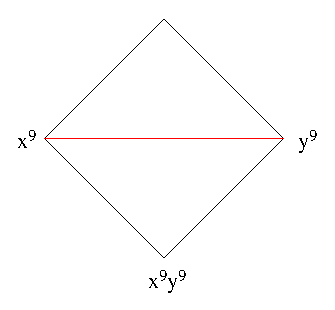
\includegraphics[width=2.5in]{TensorQuad5_Gauss}
%\caption{Pascal's triangle depiction of integrand monomial coverage 
%for two dimensions and Gaussian tensor-product quadrature order = 5.
%Red line depicts maximal total-order integrand coverage.}
%\label{fig:pascal_tensor_quad5_Gauss}
%\end{center}
%\end{figure} 

In~\cite{Eld09a}, it is demonstrated that close synchronization of
expansion form with the monomial resolution of a particular numerical
integration technique can result in significant performance
improvements.  In particular, the traditional approach of exploying a
total-order PCE (Eqs.~\ref{eq:to_multi_index}--\ref{eq:num_to_terms})
neglects a significant portion of the monomial coverage for a
tensor-product quadrature approach, and one should rather employ a
tensor-product PCE (Eqs.~\ref{eq:tp_multi_index}--\ref{eq:num_tp_terms}) 
to provide improved synchronization and more effective usage of the
Gauss point evaluations.  When the quadrature points are standard
Gauss rules (i.e., no Clenshaw-Curtis, Gauss-Patterson, or
Genz-Keister nested rules), it has been shown that tensor-product PCE
and SC result in identical polynomial forms~\cite{ConstTPQ},
completely eliminating a performance gap that exists between
total-order PCE and SC~\cite{Eld09a}.


\subsubsection{Smolyak sparse grids} \label{uq:expansion:spectral_sparse}

% For m = max points per dim, w = level:
%   Gaussian Smolyak: m = 2^(w+1) - 1  -->  m = 1, 3, 7, 15, 31, 63, 127
%   Clenshaw-Curtis:  m = 2^w     + 1  -->  m = 1, 3, 5,  9, 17, 33,  65
% TP logic would use:
%   Gaussian Smolyak: 2p <= 2m-1
%   Clenshaw-Curtis:  2p <=  m+1
% SG order selection instead using 2p <= m,
% as this is what has been observed thus far.

If the number of random variables is moderately large, one should rather
consider sparse tensor product spaces as first proposed by Smolyak
\cite{Smolyak_63} and further investigated by Refs.~\cite{gerstner_griebel_98,barth_novak_ritter_00,Fran_Schwab_Todor_04,Xiu_Hesthaven_05, webster1, webster2}
that reduce dramatically the number of collocation points, while
preserving a high level of accuracy.

Here we follow the notation and extend the description in
Ref.~\cite{webster1} to describe the Smolyak {\it isotropic} formulas
$\mathscr{A}({\rm w},n)$, where ${\rm w}$ is a level that is independent of
dimension\footnote{Other common formulations use a dimension-dependent
level $q$ where $q \geq n$.  We use $w = q - n$, where $w \geq 0$ for
all $n$.}.  The Smolyak formulas are just linear combinations of the
product formulas in Eq.~\ref{eq:multi_tensor} with the following key
property: only products with a relatively small number of points are
used.  With $\mathscr{U}^0 = 0$ and for $i \geq 1$ define
%
\begin{equation}\label{eq:delta}
\Delta^i = \mathscr{U}^i-\mathscr{U}^{i-1}.
\end{equation}
%

and we set $|\mathbf{i}| = i_1+\cdots + i_n$.
Then the isotropic Smolyak quadrature formula is given by
%
\begin{equation}\label{eq:smolyak1}
\mathscr{A}({\rm w},n) = \sum_{|\mathbf{i}| \leq {\rm w}+n}\left(\Delta^{i_1}\otimes\cdots\otimes\Delta^{i_n}\right).
\end{equation}
%
Equivalently, formula Eq.~\ref{eq:smolyak1} can be written as~\cite{was_woz}
%
\begin{equation}\label{eq:smolyak2}
\mathscr{A}({\rm w},n) = \sum_{{\rm w}+1 \leq |\mathbf{i}| \leq {\rm w}+n}(-1)^{{\rm w}+n-|\mathbf{i}|}
{n-1 \choose {\rm w}+n-|\mathbf{i}|}\cdot
\left(\mathscr{U}^{i_1}\otimes\cdots\otimes\mathscr{U}^{i_n}\right).
\end{equation}

For each index set $\mathbf{i}$ of levels, linear or nonlinear growth
rules are used to define the corresponding one-dimensional quadrature
orders.  The following growth rules are employed for indices $i \geq
1$, where closed and open refer to the inclusion and exclusion of the
bounds within an interval, respectively:
% The following is more precisely presented by replacing w with i-1
%\begin{eqnarray}
%{\rm Clenshaw-Curtis:}~~m &=& 
%\left\{ \begin{array}{ll}
%         1       & w=0 \\
%         2^w + 1 & w \geq 1 
%        \end{array} \right.        \label{eq:growth_CC_nonlin} \\
%{\rm Gaussian:}~~m &=& 2^{w+1} - 1 \label{eq:growth_Gauss_nonlin}
%\end{eqnarray}
\begin{eqnarray}
{\rm closed~nonlinear:}~~m &=& 
\left\{ \begin{array}{ll}
         1       & i=1 \\
         2^{i-1} + 1 & i > 1 
        \end{array} \right.    \label{eq:growth_CC_nonlin} \\
{\rm open~nonlinear:}~~m &=& 2^i - 1 \label{eq:growth_Gauss_nonlin} \\
{\rm open~linear:}   ~~m &=& 2 i - 1 \label{eq:growth_Gauss_lin}
\end{eqnarray}
Nonlinear growth rules are used for fully nested rules (e.g.,
Clenshaw-Curtis is closed fully nested and Gauss-Patterson is open
fully nested), and linear growth rules are best for standard Gauss
rules that take advantage of, at most, ``weak'' nesting (e.g., reuse
of the center point).
%For fully nested quadrature rules such as Clenshaw-Curtis and
%%Gauss-Patterson, nonlinear growth rules are strongly preferred
%(Eq.~\ref{eq:growth_CC_nonlin} for the former and
%Eq.~\ref{eq:growth_Gauss_nonlin} for the latter).  For at most weakly
%nested Gaussian quadrature rules, either linear or nonlinear rules may
%be selected, with the former motivated by finer granularity of control
%and uniform integrand coverage and the latter motivated by consistency
%with Clenshaw-Curtis and Gauss-Patterson.  The $m = 2i - 1$ linear
%rule takes advantage of weak nesting (e.g., Gauss-Hermite and
%Gauss-Legendre), whereas non-nested rules (e.g., Gauss-Laguerre) could
%alternatively employ an $m = i$ linear rule without any loss of reuse.
%In the experiments to follow, Clenshaw-Curtis employs nonlinear growth
%via Eq.~\ref{eq:growth_CC_nonlin}, and all Gaussian rules employ
%either nonlinear growth from Eq.~\ref{eq:growth_Gauss_nonlin} or
%linear growth from Eq.~\ref{eq:growth_Gauss_lin}.

Examples of isotropic sparse grids, constructed from the fully nested 
Clenshaw-Curtis abscissas %described in Section \ref{sub:cc}, 
and the weakly-nested Gaussian abscissas %in Section \ref{sub:cc_gauss}, 
are shown in Figure \ref{fig:isogrid_N2_q7}, where $\Omega=[-1,1]^2$
and both Clenshaw-Curtis and Gauss-Legendre employ nonlinear
growth\footnote{We prefer linear growth for Gauss-Legendre, but employ
nonlinear growth here for purposes of comparison.} from
Eqs.~\ref{eq:growth_CC_nonlin} and~\ref{eq:growth_Gauss_nonlin},
respectively.  There, we consider a two-dimensional parameter space
and a maximum level ${\rm w}=5$ (sparse grid $\mathscr{A}(5,2)$).  To
see the reduction in function evaluations with respect to full tensor
product grids, we also include a plot of the corresponding
Clenshaw-Curtis isotropic full tensor grid having the same maximum
number of points in each direction, namely $2^{\rm w}+1 = 33$.
%Whereas an isotropic tensor-product quadrature scales as $m^n$, an
%isotropic sparse grid scales as $m^{{\rm log}~n}$, significantly
%mitigating the curse of dimensionality.
%
\begin{figure}[h!]
%\vspace{-2cm}
\begin{center}
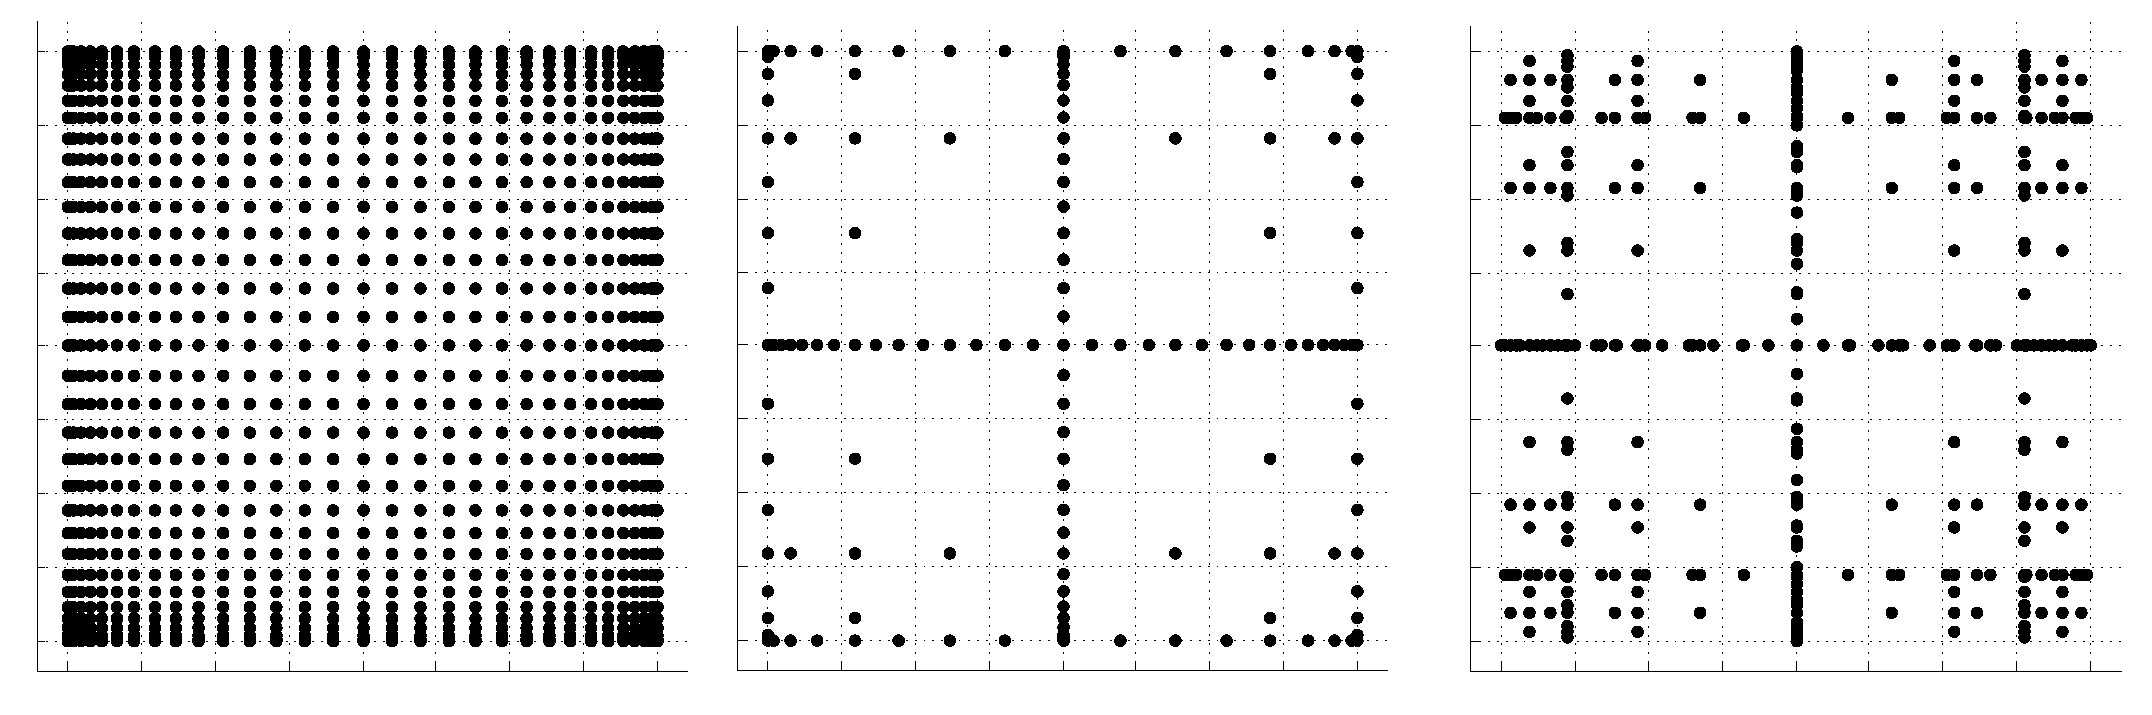
\includegraphics[width=6.5in]{images/isogrid_N2_q6}
\caption{Two-dimensional grid comparison with a tensor product grid
  using Clenshaw-Curtis points (left) and sparse grids
  $\mathscr{A}(5,2)$ utilizing Clenshaw-Curtis (middle) and
  Gauss-Legendre (right) points with nonlinear growth. }
\label{fig:isogrid_N2_q7}
\end{center}
\end{figure}

%Figure~\ref{fig:pascal_sparse_lev4_Gauss} depicts the monomial
%coverage in Pascal's triangle for two-dimensional level 4 isotropic
%sparse grids ($\mathscr{A}(4,2)$) employing the same one-dimensional
%Gaussian integration rule, where
%Figure~\ref{fig:pascal_sparse_lev4_Gauss}(a) shows the application of
%a nonlinear growth rule as given in Eq.~\ref{eq:growth_Gauss_nonlin}
%and Figure~\ref{fig:pascal_sparse_lev4_Gauss}(b) shows the use of a
%linear growth rule as given in Eq.~\ref{eq:growth_Gauss_lin}.  Using
%this geometric interpretation, subtracted tensor-product grids from
%Eqs.~\ref{eq:delta} and \ref{eq:smolyak2} can be interpreted as
%regions of overlap where only a single contribution to the integral
%should be retained.  And for these monomial coverage patterns, the
%traditional approach of exploying a total-order PCE (maximal
%resolvable total-order integrand depicted with red horizontal line)
%can be seen to be well synchronized for the case of linear growth
%rules (since only a few small ``teeth'' protrude beyond the maximal
%total-order basis) and to be somewhat conservative for nonlinear
%growth rules due to the ``hyperbolic cross'' shape (since the maximal
%total-order basis is dictated by the concave interior, neglecting the
%extended coverage along the axes).
%
%However, the inclusion of additional terms beyond the
%total-order basis in the nonlinear growth rule case, as motivated by
%the legs in Figure~\ref{fig:pascal_sparse_lev4_Gauss}(a), would be
%error-prone, since the order of the unknown response function will
%tend to push the product integrand (Eq.~\ref{eq:coeff_extract}) out
%into the concave interior, resulting in product polynomials that are
%not resolvable by the sparse integration.
%\begin{figure}[htbp]
%  \begin{subfigmatrix}{2}
%  \subfigure[Nonlinear growth rule.]{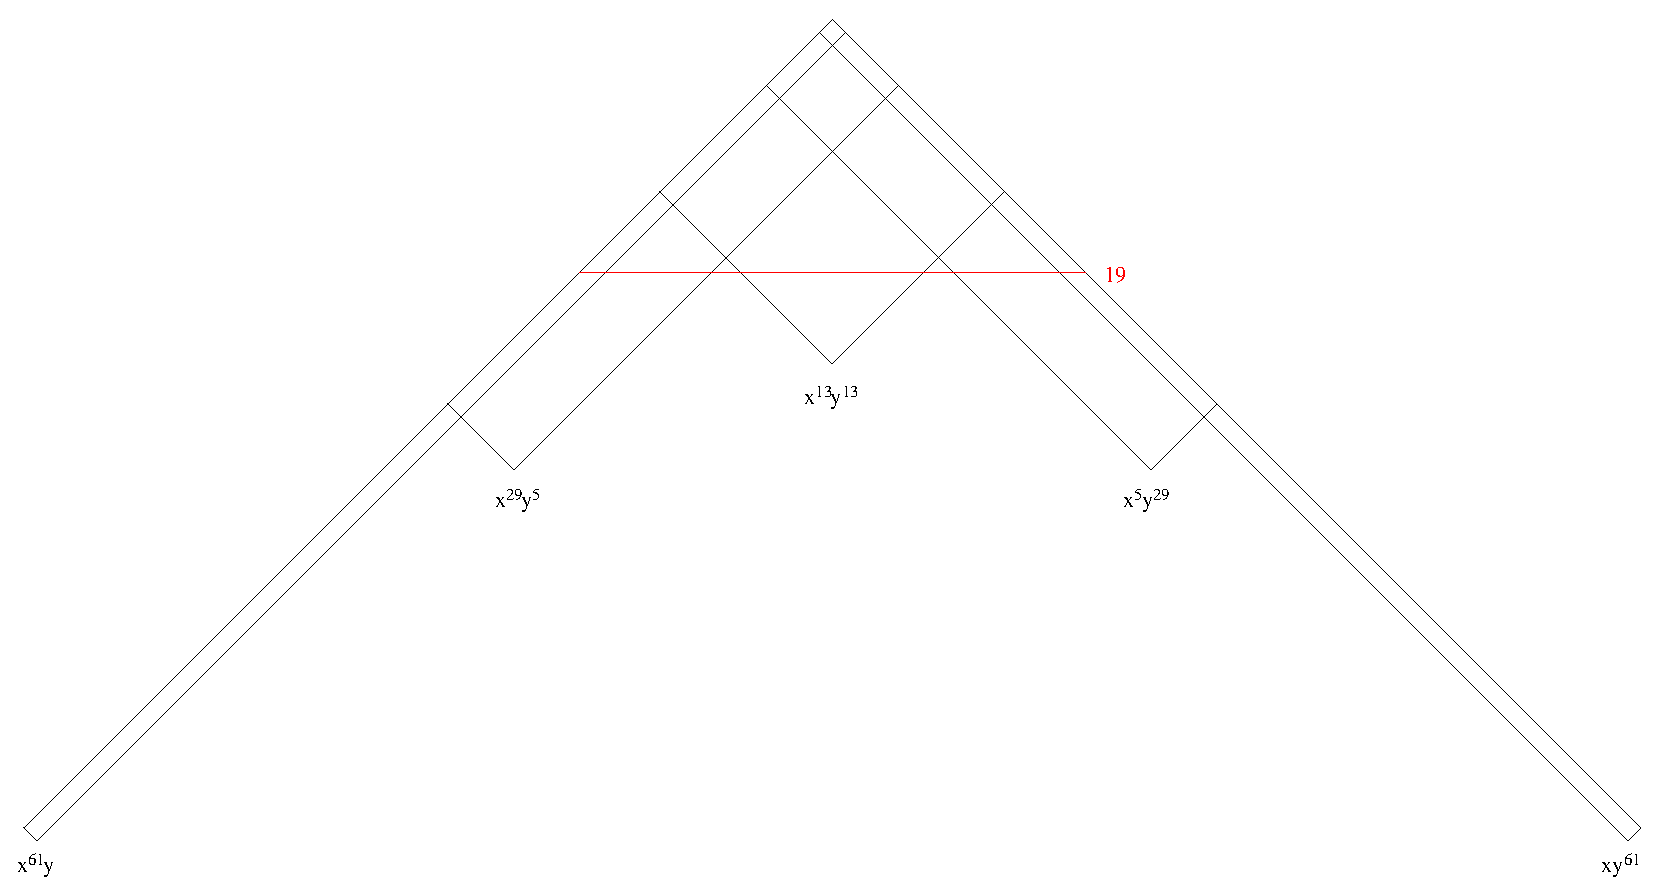
\includegraphics{SparseLevel4_NonlinGauss}}
%  \subfigure[Linear growth rule.]{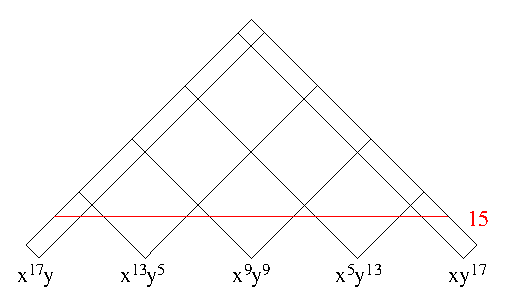
\includegraphics{SparseLevel4_LinGauss}}
%  \end{subfigmatrix}
%  \caption{Pascal's triangle depiction of integrand monomial coverage 
%for two dimensions and Gaussian sparse grid level = 4.  Red line depicts 
%maximal total-order integrand coverage.}
%\label{fig:pascal_sparse_lev4_Gauss}
%\end{figure}
%For the total-order PCE basis, the integrand monomial coverage must
%again resolve $2p$, such that $p = 9$ would be selected in this
%nonlinear growth rule example and $p = 7$ would be selected in the
%linear growth rule example.

In~\cite{Eld09a}, it is demonstrated that the synchronization of
total-order PCE with the monomial resolution of a sparse grid is
imperfect, and that sparse grid SC consistently outperforms sparse
grid PCE when employing the sparse grid to directly evaluate the
integrals in Eq.~\ref{eq:coeff_extract}.  In our DAKOTA implementation, we 
depart from the use of sparse integration of total-order expansions, and 
instead employ a linear combination of tensor expansions~\cite{ConstSSG}.
%That is, instead of employing the sparse grid as a separate numerical
%integration scheme for evaluations of Eq.~\ref{eq:coeff_extract} (for 
%which expansion synchronization is a challenge), we instead 
That is, we compute separate tensor polynomial chaos expansions for
each of the underlying tensor quadrature grids (for which there is no
synchronization issue) and then sum them using the Smolyak
combinatorial coefficient (from Eq.~\ref{eq:smolyak2} in the isotropic
case).  This improves accuracy, preserves the PCE/SC consistency
property described in Section~\ref{uq:expansion:spectral_quad}, and also
simplifies PCE for the case of anisotropic sparse grids described next.

For anisotropic Smolyak sparse grids, a dimension preference vector is
used to emphasize important stochastic dimensions.  
%A natural mechanism for quantifying
%dimension importance is through the global sensitivity analysis
%procedure described in Section~\ref{sec:ssa:global}, as the
%attribution of output variance among input sources provides an
%intuitive measure of importance in the stochastic setting.
Given a mechanism for defining anisotropy, we can extend the
definition of the sparse grid from that of Eq.~\ref{eq:smolyak2} to
weight the contributions of different index set components.  First,
the sparse grid index set constraint becomes
\begin{equation}
{\rm w}\underline{\gamma} < \mathbf{i} \cdot \mathbf{\gamma} \leq 
{\rm w}\underline{\gamma}+|\mathbf{\gamma}|
\label{eq:aniso_smolyak_constr}
\end{equation}
where $\underline{\gamma}$ is the minimum of the dimension weights
$\gamma_k$, $k$ = 1 to $n$.  The dimension weighting vector
$\mathbf{\gamma}$ amplifies the contribution of a particular dimension
index within the constraint, and is therefore inversely related to the
dimension preference (higher weighting produces lower index set
levels).  For the isotropic case of all $\gamma_k = 1$, it is evident
that you reproduce the isotropic index constraint ${\rm w}+1 \leq
|\mathbf{i}| \leq {\rm w}+n$ (note the change from $<$ to $\leq$).
Second, the combinatorial coefficient for adding the contribution from
each of these index sets is modified as described in~\cite{Burk09}.
%Given the modified index sets and combinatorial coefficients defined
%from the dimension preference vector, interpolation (SC) on
%anisotropic sparse grids proceeds as for the isotropic case.  PCE,
%however, again has the challenge of expansion tailoring.  Fortunately,
%in the anistropic case, we can assume that more is known about the
%form of the response function (especially if the dimension preference
%was based on variance-based decomposition).  This allows us to abandon
%the safe total-order basis approach in favor of a tightly-synchronized
%expansion formulation that applies the $2p$ logic to all of the
%protruding ``legs'' in the monomial resolution structure.


\subsubsection{Cubature} \label{uq:expansion:cubature}

Cubature rules~\cite{stroud,xiu_cubature} are specifically optimized
for multidimensional integration and are distinct from tensor-products 
and sparse grids in that they are not based on combinations of 
one-dimensional Gauss quadrature rules.  They have the advantage of 
improved scalability to large numbers of random variables, but are 
restricted in integrand order and require homogeneous random variable 
sets (achieved via transformation).  For example, optimal rules for
integrands of 2, 3, and 5 and either Gaussian or uniform densities 
allow low-order polynomial chaos expansions ($p=1$ or $2$) that are 
useful for global sensitivity analysis including main effects and, 
for $p=2$, all two-way interactions.


\subsection{Linear regression} \label{uq:expansion:regress}

The linear regression approach uses a
single linear least squares solution of the form:
\begin{equation}
\boldsymbol{\Psi} \boldsymbol{\alpha} = \boldsymbol{R} \label{eq:regression}
\end{equation}
to solve for the complete set of PCE coefficients
$\boldsymbol{\alpha}$ that best match a set of response values
$\boldsymbol{R}$.  The set of response values is obtained either by
performing a design of computer experiments within the density
function of $\boldsymbol{\xi}$ (point
collocation~\cite{pt_colloc1,pt_colloc2}) or from a subset of tensor
quadrature points with highest product weight (probabilistic
collocation~\cite{Tat95}).  In either case, each row of the matrix
$\boldsymbol{\Psi}$ contains the $N_t$ multivariate polynomial terms
$\Psi_j$ evaluated at a particular $\boldsymbol{\xi}$ sample.  An
over-sampling is recommended in the case of random samples
(\cite{pt_colloc2} recommends $2N_t$ samples), resulting in a least
squares solution for the over-determined system.  As for
sampling-based coefficient estimation, this approach is only valid for
PCE and does not require synchronization with monomial coverage; thus
it is common to combine this coefficient estimation approach with a
traditional total-order chaos expansion in order to keep sampling
requirements low.  In this case, simulation requirements for this
approach scale as $\frac{r(n+p)!}{n!p!}$ ($r$ is an over-sampling
factor with typical values $1 \leq r \leq 2$), which can be
significantly more affordable than isotropic tensor-product quadrature
(scales as $(p+1)^n$ for standard Gauss rules) for larger problems.
%A closely related technique is known as the ``probabilistic
%collocation'' approach.  Rather than employing random over-sampling,
%this technique uses a selected subset of $N_t$ Gaussian quadrature
%points (those with highest tensor-product weighting), which provides
%more optimal collocation locations and preserves interpolation
%properties.
Finally, additional regression equations can be obtained through the
use of derivative information (gradients and Hessians) from each
collocation point, which can aid in scaling with respect to the number
of random variables, particularly for adjoint-based derivative
approaches.


\subsection{Analytic moments} \label{uq:expansion:moment}

Mean and covariance of polynomial chaos expansions are available
in simple closed form:
\begin{eqnarray}
\mu_i      &=& \langle R_i \rangle ~~\cong~~ \sum_{k=0}^P \alpha_{ik} \langle 
\Psi_k(\boldsymbol{\xi}) \rangle ~=~ \alpha_{i0} \label{eq:mean_pce} \\
\Sigma_{ij} &=& \langle (R_i - \mu_i)(R_j - \mu_j) \rangle ~~\cong~~ 
%\langle (\sum_{j=1}^P \alpha_j \Psi_j(\boldsymbol{\xi}))^2 \rangle ~=~ 
\sum_{k=1}^P \sum_{l=1}^P \alpha_{ik} \alpha_{jl}
\langle \Psi_k(\boldsymbol{\xi}) \Psi_l(\boldsymbol{\xi}) \rangle ~=~
\sum_{k=1}^P \alpha_{ik}\alpha_{jk} \langle \Psi^2_k \rangle~~~~~~~~ \label{eq:covar_pce} 
\end{eqnarray}
where the norm squared of each multivariate polynomial is computed
from Eq.~\ref{eq:norm_squared}.  These expressions provide exact moments 
of the expansions, which converge under refinement to moments of the 
true response functions.
%Higher moments are also available
%analytically and could be employed in moment fitting approaches (i.e.,
%Pearson and Johnson models) in order to approximate a response PDF,
%although this is outside the scope of the current paper.

Similar expressions can be derived for stochastic collocation:
\begin{eqnarray}
\mu_i      &=& \langle R_i \rangle ~~\cong~~ \sum_{k=1}^{N_p} r_{ik} \langle 
\boldsymbol{L}_k(\boldsymbol{\xi}) \rangle ~=~ \sum_{k=1}^{N_p} r_{ik} w_k 
\label{eq:mean_sc} \\
\Sigma_{ij} &=& \langle R_i R_j \rangle - \mu_i \mu_j
~~\cong~~ \sum_{k=1}^{N_p} \sum_{l=1}^{N_p} r_{ik} r_{jl} \langle
\boldsymbol{L}_k(\boldsymbol{\xi}) \boldsymbol{L}_l(\boldsymbol{\xi}) \rangle
- \mu_i \mu_j ~=~ \sum_{k=1}^{N_p} r_{ik} r_{jk} w_k - \mu_i \mu_j~~~~~~~~~ \label{eq:covar_sc} 
\end{eqnarray}
where we have simplified the expectation of Lagrange polynomials
constructed at Gauss points and then integrated at these same Gauss
points.  For tensor grids and sparse grids with fully nested rules,
these expectations leave only the weight corresponding to the point
for which the interpolation value is one, such that the final
equalities in Eqs.~\ref{eq:mean_sc}--\ref{eq:covar_sc} hold precisely.
For sparse grids with non-nested rules, however, interpolation error
exists at the collocation points, such that these final equalities
hold only approximately.  In this case, we have the choice of
computing the moments based on sparse numerical integration or based
on the moments of the (imperfect) sparse interpolant, where small
differences may exist prior to numerical convergence.  In DAKOTA, we
employ the former approach; i.e., the right-most expressions in
Eqs.~\ref{eq:mean_sc}--\ref{eq:covar_sc} are employed for all tensor
and sparse cases irregardless of nesting.  Skewness and kurtosis
calculations as well as sensitivity derivations in the following
sections are also based on this choice.
%Similarly, moment $k$ for stochastic collocation is just 
%$\sum_{j=1}^{N_p} r^k_j w_j$ minus previously computed moments.
The expressions for skewness and (excess) kurtosis from direct numerical 
integration of the response function are as follows:
\begin{eqnarray}
\gamma_{1_i} &=& \left\langle \left(\frac{R_i - \mu_i}{\sigma_i}\right)^3 \right\rangle
~~\cong~~ \frac{1}{\sigma_i^3} \left[ \sum_{k=1}^{N_p} (r_{ik}-\mu_i)^3 w_k \right] \label{eq:skewness} \\
\gamma_{2_i} &=& \left\langle \left(\frac{R_i - \mu_i}{\sigma_i}\right)^4 \right\rangle - 3 
~~\cong~~ \frac{1}{\sigma_i^4} \left[ \sum_{k=1}^{N_p} (r_{ik}-\mu_i)^4 w_k \right] - 3\label{eq:kurtosis} 
\end{eqnarray}


\subsection{Local sensitivity analysis: derivatives with respect to expansion variables} \label{uq:expansion:rvsa}

Polynomial chaos expansions are easily differentiated with respect to
the random variables~\cite{reagan_sens}.  First, using
Eq.~\ref{eq:pc_exp_trunc},
\begin{equation}
\frac{dR}{d\xi_i} = \sum_{j=0}^P \alpha_j 
\frac{d\Psi_j(\boldsymbol{\xi})}{d\xi_i}\label{eq:dR_dxi_pce}
\end{equation}
and then using Eq.~\ref{eq:multivar_prod}, 
\begin{equation}
\frac{d\Psi_j(\boldsymbol{\xi})}{d\xi_i} = \frac{d\psi_i}{d\xi_i}
\prod_{\stackrel{\scriptstyle k=1}{k \ne i}}^n \psi_{m_k^j}(\xi_k)
\label{eq:deriv_prod_pce}
\end{equation}
where the univariate polynomial derivatives $\frac{d\psi_i}{d\xi_i}$
have simple closed form expressions for each polynomial in the Askey
scheme~\cite{abram_stegun}.  Finally, using the Jacobian of the
(extended) Nataf variable transformation,
\begin{equation}
\frac{dR}{dx_i} = \frac{dR}{d\boldsymbol{\xi}} 
\frac{d\boldsymbol{\xi}}{dx_i} \label{eq:dR_dx}
\end{equation}
which simplifies to $\frac{dR}{d\xi_i} \frac{d\xi_i}{dx_i}$ in the
case of uncorrelated $x_i$.  

Similar expressions may be derived for stochastic collocation, starting
from Eq.~\ref{eq:sc_exp_short}:
\begin{equation}
\frac{dR}{d\xi_i} = \sum_{j=1}^{N_p} r_j 
\frac{d\boldsymbol{L}_j(\boldsymbol{\xi})}{d\xi_i}\label{eq:dR_dxi_sc}
\end{equation}
where the multidimensional interpolant $\boldsymbol{L}_j$ is formed
over either tensor-product quadrature points or a Smolyak sparse grid.
For the former case, the derivative of the multidimensional
interpolant $\boldsymbol{L}_j$ involves a product rule of the
one-dimensional interpolants $L_k$:
\begin{equation}
\frac{d\boldsymbol{L}_j(\boldsymbol{\xi})}{d\xi_i} = \frac{dL_i}{d\xi_i}
\prod_{\stackrel{\scriptstyle k=1}{k \ne i}}^n L_k(\xi_k)
\label{eq:deriv_prod_sc}
\end{equation}
and for the latter case, the derivative involves a linear combination
of these product rules, as dictated by the Smolyak recursion shown in
Eq.~\ref{eq:smolyak2}.  Finally, calculation of $\frac{dR}{dx_i}$
involves the same Jacobian application shown in Eq.~\ref{eq:dR_dx}.

\subsection{Global sensitivity analysis: variance-based decomposition}\label{uq:expansion:vbd}

In addition to obtaining derivatives of stochastic expansions with 
respect to the random variables, it is possible to obtain 
variance-based sensitivity indices from the stochastic expansions. 
Variance-based sensitivity indices are explained in 
Section~\ref{dace:sensitivity}.  The concepts are summarized here 
as well.  Variance-based decomposition 
is a global sensitivity method that summarizes how the uncertainty 
in model output can be apportioned to uncertainty in individual 
input variables.  VBD uses two primary measures, the main effect 
sensitivity index $S_{i}$ and the total effect index $T_{i}$.  These 
indices are also called the Sobol' indices. The main effect sensitivity 
index corresponds to the fraction of the uncertainty in the output, $Y$, 
that can be attributed to input $x_{i}$ alone.  The total effects index 
corresponds to the fraction of the uncertainty in 
the output, $Y$, that can be attributed to input $x_{i}$ and its 
interactions with other variables. The main effect sensitivity index
compares the variance of the conditional expectation
$Var_{x_{i}}[E(Y|x_{i})]$ against the total variance $Var(Y)$.
Formulas for the indices are: 

\begin{equation}
S_{i}=\frac{Var_{x_{i}}[E(Y|x_{i})]}{Var(Y)} \label{eq:sobol}
\end{equation}

and 
\begin{equation}
T_{i}=\frac{E(Var(Y|x_{-i}))}{Var(Y)}=\frac{Var(Y)-Var(E[Y|x_{-i}])}{Var(Y)}
\label{eq:total_sobol}
\end{equation}

where $Y=f({\bf x})$ and ${x_{-i}=(x_{1},...,x_{i-1},x_{i+1},...,x_{m})}$.

The calculation of $S_{i}$ and $T_{i}$ requires the evaluation of 
m-dimensional integrals which are typically approximated by Monte-Carlo 
sampling. However, in stochastic expansion methods, it is possible to 
obtain the sensitivity indices as analytic functions of the 
coefficients in the stochastic expansion.  The derivation 
of these results is presented in ~\cite{Tang10b}. The sensitivity 
indices are printed as a default when running either 
polynomial chaos or stochastic collocation in DAKOTA. 
Note that in addition to the first-order main effects, $S_{i}$, 
we are able to calculate the sensitivity indices for higher order 
interactions such as the two-way interaction  $S_{i,j}$.   

\subsection{Automated Refinement}\label{uq:expansion:refine}

Several approaches for refinement of stochastic expansions are
presented here: uniform p-refinement, adaptive p-refinement using
anisotropic sparse and tensor grids, and goal-oriented adaptive
p-refinement using generalized sparse grids.  %Each involves
%incrementing the grid upon which the expansions are based, using a
%variety of criteria.

\subsubsection{Uniform p-refinement}

Uniform p-refinement involves ramping the order of a tensor-product
quadrature grid or the level of a Smolyak sparse grid isotropically,
that is, with no dimension preference.  In this case, Sobol' indices
are not employed, and the only algorithmic requirements are:
\begin{itemize}
\item With the usage of nested integration rules and ``restricted growth''
  schemes that attempt to reduce inefficiency due to the hyperbolic
  cross phenomenon, one must ensure that a change in level results in
  an adequate change in the grid.  If it does not, continue
  incrementing the order/level (without grid evaluation) until
  sufficient change is obtained.  An insufficient grid change is 
  likely to cause premature convergence in the refinement process.
\item A convergence criterion is required.  One useful general-purpose
  metric is the $L^2$ norm of the change in the response covariance matrix.
\end{itemize}


\subsubsection{Adaptive p-refinement}

Adaptive p-refinement involves ramping the order of a tensor-product
quadrature grid or the level of a Smolyak sparse grid anisotropically,
that is, using a defined dimension preference.  This dimension
preference may be computed from local sensitivity analysis, global
sensitivity analysis, a posteriori error estimation, or decay rate
estimation.  Herein, we focus on global sensitivity analysis
from low order isotropic expansions where dimension preference is
defined from total Sobol' indices (Eq.~\ref{eq:total_sobol}) and is
updated on every iteration.  These main effects admit anisotropic
sparse grids based on a linear index-set constraint
(Eq.~\ref{eq:aniso_smolyak_constr}).%; with the introduction of
%interaction effects, nonlinear index-set constraints can also be
%considered.


\subsubsection{Goal-oriented p-refinement}

If the objectives and constraints of a design under uncertainty
problem are focused on variance (e.g., robust design), then the
general-purpose formulations described above are sufficiently
goal-oriented.  However, for other classes of problems (e.g.,
reliability-based design or stochastic inverse problems), we may
prefer to employ refinement approaches guided by assessments of
accuracy in other statistical quantities of interest.  %A particular
%focus in this effort is to refine adaptively with the goal of accuracy
%in tail probability estimates.  There are two parts to this effort:
%goal-oriented p-refinement using generalized sparse grids and
%efficient tail probability estimation.

%Since probability levels are not available analytically from
%stochastic expansions, they must be evaluated numerically using some
%form of sampling on the expansion.  For tail probability estimates,
%standard sampling approaches (e.g., LHS) can become expensive even for
%this surrogate-based sampling and we require a more directed
%probability estimation procedure, in particular the importance
%sampling procedure described previously in Section~\ref{sec:imp_samp}.

Given a capability to estimate alternative goals, we must then employ
an adaptive refinement procedure that flexibly accommodates these
goals.  The generalized sparse grid
algorithm~\cite{Gerstner_Griebel_2003}, originally intended for
adaptive numerical integration, is readily adapted to the adaptive
refinement of PCE and SC expansions.  Customizations of the DAKOTA 
approach from that of~\cite{Gerstner_Griebel_2003} include:
\begin{itemize}
\item In addition to hierarchical interpolants in SC, we employ
  independent polynomial chaos expansions for each active and accepted
  index set.  Pushing and popping index sets then involves increments
  of tensor chaos expansions (as described in
  Section~\ref{uq:expansion:spectral_sparse}) along with corresponding
  increments to the Smolyak combinatorial coefficients.
\item Since we support bases for more than uniform and normal random
  variables, we exploit rule nesting when possible (i.e.,
  Gauss-Patterson for uniform or transformed uniform variables, and
  Genz-Keister for normal or transformed normal variables), but we do
  not require it.  This implies a loss of some algorithmic 
  simplifications that occur when grids are strictly hierarchical.
\item In the evaluation of the effect of a trial index set, the goal
  in~\cite{Gerstner_Griebel_2003} is numerical integration and the 
  metric is the size of the increment
  induced by the trial set on the expectation of the function of
  interest.  It is straightforward to instead measure the effect of a
  trial index set on response covariance, numerical probability, or
  other statistical quantities of interest (QOI) computed by
  post-processing the resulting PCE or SC expansion (it is much 
  less straightforward to embed QOI in the calculation of dimension
  preference for anisotropic tensor/sparse grids).
\end{itemize}

Given these customizations, the algorithmic steps can be summarized as:
\begin{enumerate}
\item {\em Initialization:} Starting from an initial isotropic or
  anisotropic reference grid (often the $w=0$ grid corresponding to a
  single collocation point), accept the reference index sets as the
  old set and define active index sets using the admissible forward
  neighbors of all old index sets.
\item {\em Trial set evaluation:} Evaluate the tensor grid
  corresponding to each trial active index set, form the tensor
  polynomial chaos expansion corresponding to it, update the Smolyak
  combinatorial coefficients, and combine the trial expansion with the
  reference expansion.  Perform necessary bookkeeping to allow
  efficient restoration of previously evaluated tensor polynomial
  chaos expansions.
\item {\em Trial set selection:} Select the trial index set that
  induces the largest change in the statistical quantity of interest.
  In our studies, we employ an $L^2$ norm of change in
  probaility/reliability/response level mappings, when level mappings
  are present, or $L^2$ norm of change in response covariance, when
  level mappings are not present.
\item {\em Update sets:} If the largest change induced by the trial
  sets exceeds a specified convergence tolerance, then promote the
  selected trial set from the active set to the old set and update the
  active sets with new admissible forward neighbors; return to step 2.
  If the convergence tolerance is satisfied, advance to step 5.
\item {\em Finalization:} Promote all remaining active sets to the old
  set, update the Smolyak combinatorial coefficients, and perform a
  final combination of tensor expansions to arrive at the final result
  for the statistical quantity of interest.
\end{enumerate}


\subsection{Uncertainty Quantification Example using Stochastic Collocation}\label{uq:uncertainty2}

A typical DAKOTA input file for performing an uncertainty
quantification using polynomial chaos expansions is shown in the
Tutorial Chapter,
Section~\ref{tutorial:example:uncert_quant:poly_chaos}.  The example
in the Tutorial Chapter illustrates PCE built on anisotropic tensor
product quadrature.  The uncertain variables are uniforms, so the
expansion is built using classical Legendre polynomials. This section
presents a more sophisticated example, where we use stochastic
collocation built on an anisotropic sparse grid defined from
numerically-generated orthogonal polynomials.  The uncertain variables
are lognormal in this example and the orthogonal polynomials are
generated from Gauss-Wigert recursion coefficients~\cite{simpson_gw}
in combination with the Golub-Welsch procedure~\cite{GolubWelsch69}.
The input file is shown in Figure~\ref{uq:figure11}. Note that the
dimension preference of $(2,1)$ is inverted to define a $\gamma$
weighting vector of $(0.5,1)$ (and $\underline{\gamma}$ of $0.5$) for
use in Eq.~\ref{eq:aniso_smolyak_constr}.  In this example, we compute
CDF probabilities for six response levels of Rosenbrock's function.
This example requires 19 function evaluations to calculate the
interpolating polynomials in stochastic collocation and the resulting
expansion exactly reproduces Rosenbrock's function.  The placement of
the points generated by the sparse grid is shown in
Figure~\ref{uq:figure11b}.

\begin{figure}
  \centering
  \begin{bigbox}
    \begin{small}
      \verbatimtabinput[8]{dakota_sc.in}
    \end{small}
  \end{bigbox}
\caption{DAKOTA input file for performing UQ using stochastic collocation.}
\label{uq:figure11}
\end{figure}

\begin{figure}[ht!]
  \centering
  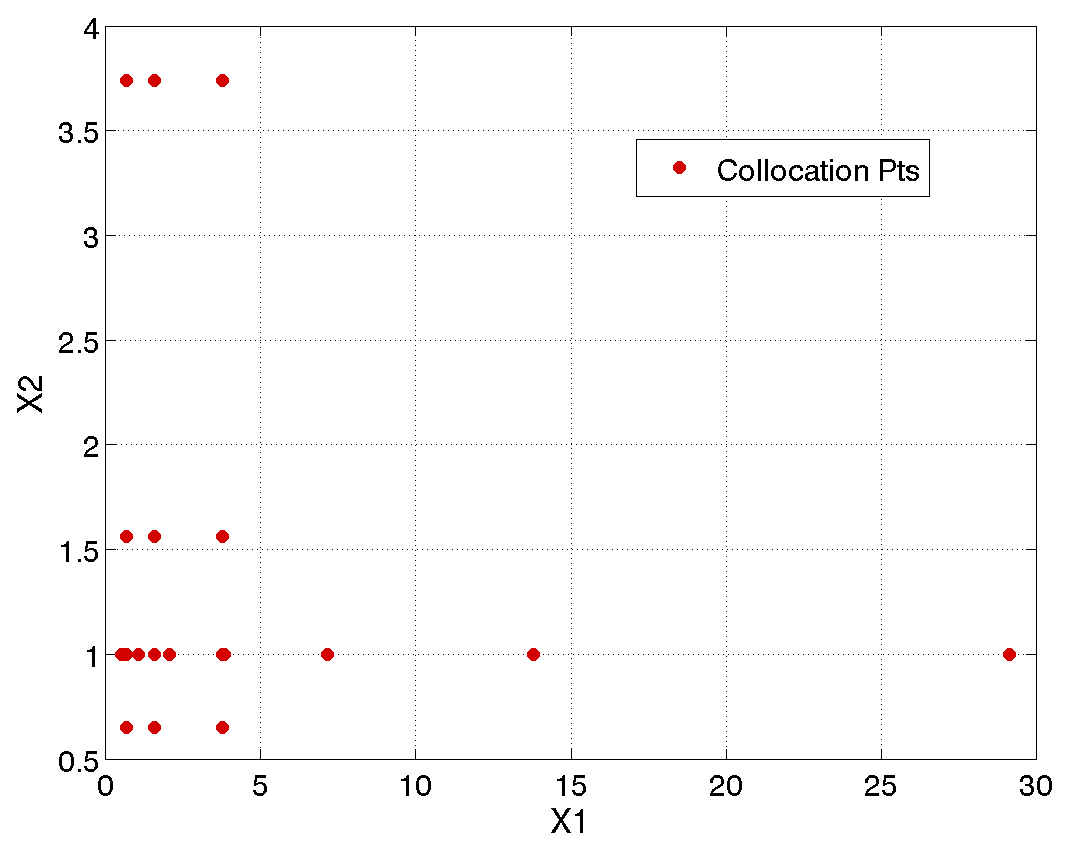
\includegraphics[height=2.5in]{images/rosen_sc_pts}
  \caption{Rosenbrock stochastic collocation example: sparse grid points.}
  \label{uq:figure11b}
\end{figure}

Once the expansion coefficients have been calculated, some statistics
are available analytically and others must be evaluated numerically.
For the numerical portion, the input file specifies the use of 10000
samples, which will be evaluated on the expansion to compute the CDF
probabilities.  In Figure~\ref{uq:figure12}, excerpts from the results
summary are presented.  We first see the analytic statistics for 
mean and standard deviation as computed from 
Eqs.~\ref{eq:mean_sc}-\ref{eq:var_sc} as well as skewness, and kurtosis.  
The response covariance (collapsing to a single variance value for 
one response function) and global sensitivity indices
(Sobol' indices) are presented next. This example shows that variable 
x1 has the largest main effect (0.99) as compared with variable 
x2 (0.0007) or the interaction between x1 and x2 (0.005). 
%After the global sensitivity indices, the local, analytic random 
%variable sensitivities are presented, as computed from
%Eqs.~\ref{eq:dR_dx}-\ref{eq:dR_dxi_sc}, evaluated at the mean values.
Finally, we see the numerical results for the CDF probabilities based
on 10000 samples performed on the expansion.  For example, the probability 
that the Rosenbrock function is less than 100 is 0.7233.  Note that these 
results are significantly different than the ones presented in 
Section~\ref{tutorial:example:uncert_quant:poly_chaos} because of 
the different assumptions about the inputs: uniform[-2,2] versus
lognormals with means of 1.0 and standard deviations of 0.5. 
\begin{figure}
\centering
\begin{bigbox}
\begin{small}
\begin{verbatim}
Statistics derived analytically from polynomial expansion:

Moment-based statistics for each response function:
                            Mean           Std Dev          Skewness          Kurtosis
 response_fn_1  2.5671972656e+02  2.0484189184e+03  2.7419241630e+02  1.9594567379e+06

Covariance among response functions:
[[  4.1960200651e+06 ]] 

Global sensitivity indices for each response function:
response_fn_1 Sobol indices:
                                  Main             Total
                      9.9391978710e-01  9.9928724777e-01 x1
                      7.1275222945e-04  6.0802128961e-03 x2
                           Interaction
                      5.3674606667e-03 x1 x2 

Statistics based on 10000 samples performed on polynomial expansion:

Level mappings for each response function:
Cumulative Distribution Function (CDF) for response_fn_1:
     Response Level  Probability Level  Reliability Index  General Rel Index
     --------------  -----------------  -----------------  -----------------
   1.0000000000e-01   1.8100000000e-02
   1.0000000000e+00   8.7800000000e-02
   5.0000000000e+01   5.8410000000e-01
   1.0000000000e+02   7.2330000000e-01
   5.0000000000e+02   9.2010000000e-01
   1.0000000000e+03   9.5660000000e-01
\end{verbatim}
\end{small}
\end{bigbox}
\caption{Excerpt of UQ output for stochastic collocation example.}
\label{uq:figure12}
\end{figure}

\section{Epistemic Nondeterministic Methods}\label{uq:epistemic}

Uncertainty quantification is often used as part of the risk
assessment of performance, reliability, and safety of engineered
systems.  Increasingly, uncertainty is separated into two categories
for analysis purposes: aleatory and epistemic
uncertainty~\cite{Obe03,Hel07}. Aleatory uncertainty is also referred to as
variability, irreducible or inherent uncertainty, or uncertainty due
to chance. Examples of aleatory uncertainty include the height of
individuals in a population, or the temperature in a processing
environment.  Aleatory uncertainty is usually modeled with probability
distributions, and sampling methods such as Latin Hypercube sampling
in DAKOTA can be used to model aleatory uncertainty. In contrast,
epistemic uncertainty refers to lack of knowledge or lack of
information about a particular aspect of the simulation model,
including the system and environment being modeled. An increase in
knowledge or information relating to epistemic uncertainty will lead
to a reduction in the predicted uncertainty of the system response or
performance. For epistemic uncertain variables, typically one does not
know enough to specify a probability distribution on a variable.
Epistemic uncertainty is referred to as subjective, reducible, or lack
of knowledge uncertainty. Examples of epistemic uncertainty include
little or no experimental data for a fixed but unknown physical
parameter, incomplete understanding of complex physical phenomena,
uncertainty about the correct model form to use, etc.

There are many approaches which have been developed to model epistemic
uncertainty, including fuzzy set theory, possibility theory, and
evidence theory. It is also possible to use simple interval analysis in 
an epistemic context.  Interval analysis and evidence theory are 
described in more detail below.

\subsection{Interval Methods for Epistemic Analysis}\label{uq:interval}
In interval analysis, one assumes that nothing is known about 
an epistemic uncertain variable except that its value lies 
somewhere within an interval.  In this situation, it is NOT 
assumed that the value has a uniform probability of occuring 
within the interval.  Instead, the interpretation is that 
any value within the interval is a possible value or a potential 
realization of that variable.  In interval analysis, the 
uncertainty quantification problem is one of determining the 
resulting bounds on the output (defining the output interval) 
given interval bounds on the inputs. Again, any output response 
that falls within the output interval is a possible output 
with no frequency information assigned to it.

We have the capability to perform interval analysis using either
\texttt{global\_interval\_est} or \texttt{local\_interval\_est}.
In the global approach, one uses either a global optimization 
method or a sampling method to assess the bounds. 
\texttt{global\_interval\_est}
allows the user to specify either \texttt{lhs}, which performs 
Latin Hypercube Sampling and takes the minimum and maximum of 
the samples as the bounds (no optimization is 
performed) or \texttt{ego}.  In the case of \texttt{ego}, 
the efficient global optimization method is used to calculate 
bounds.  The ego method is described in Section~\ref{sbm:egm}.
If the problem is amenable to local optimization 
methods (e.g. can provide derivatives or use finite difference 
method to calculate derivatives), then one can use local
methods to calculate these bounds.  \texttt{local\_interval\_est}
allows the user to specify either \texttt{sqp} which is sequential 
quadratic programming, or \texttt{nip} which is a nonlinear interior point 
method. 

Note that when performing interval analysis, it is necessary to 
define interval uncertain variables as described in 
Section~\ref{variables:uncertain}.  For interval analysis, 
one must define only one interval per input variable, in 
contrast with Dempster-Shafer evidence theory, where 
an input can have several possible intervals.  Interval 
analysis can be considered a subset of Dempster-Shafer
evidence theory where each input is defined by one 
input interval with a basic probability assignment of one. 
If you are performing a pure interval analysis, we 
recommend using either \texttt{global\_interval\_est} or 
\texttt{local\_interval\_est}.  An example of interval estimation 
is found in the test file \texttt{dakota\_uq\_cantilever\_interval.in}, 
and also in the Tutorial, Section~\ref{tutorial:example:uncert_quant:interval}. 
Note that we have kept separate 
implementations of interval analysis and Dempster-Shafer 
evidence theory because our users often want to couple 
interval analysis on an ``outer loop'' with an aleatory, 
probabilistic analysis on an ``inner loop'' for nested, 
second-order probability calculations.  See Section~\ref{models:ex:sop} 
for more details on nested approaches.


\subsection{Dempster-Shafer Theory of Evidence}\label{uq:dempshaf}
We have chosen to pursue evidence theory at Sandia as a way to 
model epistemic uncertainty, in part because evidence theory is
a generalization of probability theory.  Evidence theory is also
referred to as Dempster-Shafer theory or the theory of random
sets~\cite{Obe03}.  In evidence theory, there are two complementary
measures of uncertainty: belief and plausibility.  Together, belief
and plausibility can be thought of as defining lower and upper bounds,
respectively, on probabilities.  Belief and plausibility define the
lower and upper limits or intervals on probability values. 
Typical plots of cumulative and complementary cumulative 
belief and plausibility functions are shown in 
Figure~\ref{uq:figure15}~\cite{Hel07}.  
In evidence theory, it is not possible to specify one probability value.
Instead, there is a range of values that is consistent with the
evidence. The range of values is defined by belief and
plausibility. Note that no statement or claim is made about one value
within an interval being more or less likely than any other value.

This section focuses on Dempster-Shafer evidence theory.  We also 
use a technique called second-order probability to perform 
uncertainty quantification when there is both epistemic and 
aleatory uncertainty present.  Second-order probability is a nested 
technique with two levels of uncertainty quantification.  
The outer level UQ is typically linked 
to epistemic uncertainties and the inner level UQ is commonly associated 
with aleatory uncertainties.  A common approach used is to sample 
possible realizations of epistemic variables in the outer loop, 
then send these to the inner loop for additional sampling over the aleatory 
variables.  In this way one generates ``families'' or ensembles of 
cumulative distribution functions, where each individual CDF is based on 
aleatory uncertainty, and the ensemble is based on epistemic uncertainty. 
See Section~\ref{models:ex:sop} for more details.

\begin{figure}
  \centering 
  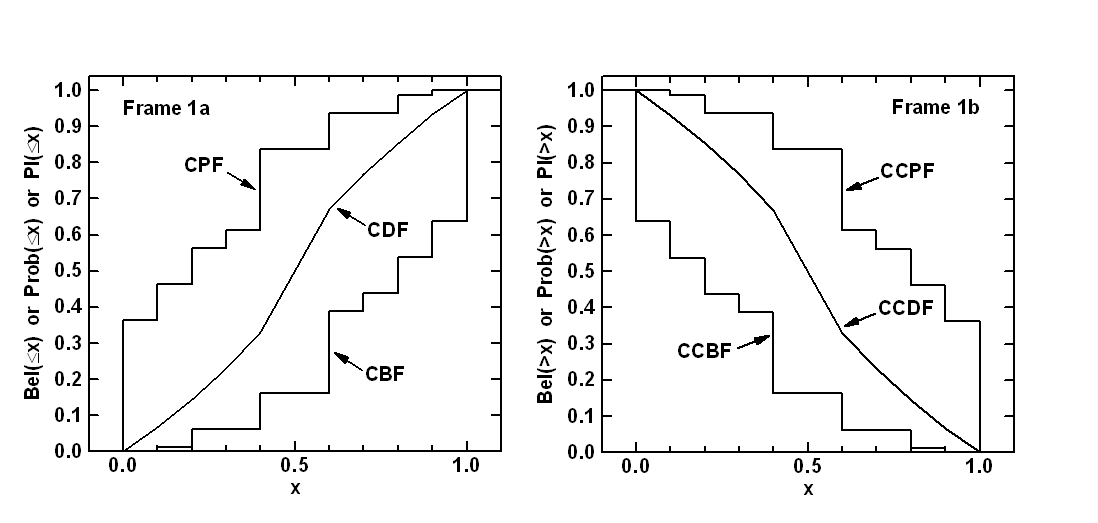
\includegraphics[scale=0.8]{images/belief_plaus} 
  \caption{Example cumulative belief and plausibility distribution functions on left; complementary cumulative belief and plausibility distribution functions on right}
  \label{uq:figure15}
\end{figure}

In Dempster-Shafer evidence theory, the uncertain input variables are
modeled as sets of intervals.  The user assigns a basic probability
assignment (BPA) to each interval, indicating how likely it is that
the uncertain input falls within the interval.  The BPAs for a
particular uncertain input variable must sum to one.  The intervals
may be overlapping, contiguous, or have gaps. In DAKOTA, an interval
uncertain variable is specified as \texttt{interval\_uncertain}.  When
one defines an interval type variable in DAKOTA, it is also necessary
to specify the number of intervals defined for each variable with
\texttt{iuv\_num\_intervals} as well the basic probability assignments
per interval, \texttt{iuv\_interval\_probs}, and the associated bounds
per each interval, \texttt{iuv\_interval\_bounds}. 
Figure~\ref{uq:figure16} shows the input specification for interval
uncertain variables.  The example shown in Figure~\ref{uq:figure16}
has two epistemic uncertain interval variables.  The first uncertain
variable has three intervals and the second has two. The basic
probability assignments for the first variable are 0.5, 0.1, and 0.4,
while the BPAs for the second variable are 0.7 and 0.3. Note that it
is possible (and often the case) to define an interval uncertain
variable with only ONE interval.  This means that you only know that
the possible value of that variable falls within the interval, and the
BPA for that interval would be 1.0.  In the case we have shown, the
interval bounds on the first interval for the first variable are 0.6
and 0.9, and the bounds for the second interval for the first variable
are 0.1 to 0.5, etc.

\begin{figure}
  \centering
  \begin{bigbox}
    \begin{small}
      \verbatimtabinput[8]{dakota_uq_textbook_dste.in}
    \end{small}
  \end{bigbox}
\caption{DAKOTA input file for UQ example using Evidence Theory.}
\label{uq:figure16}
\end{figure}

Once the intervals, the BPAs, and the interval bounds are defined, 
the user can run an epistemic analysis by specifying the method as 
either \texttt{global\_evidence} or 
\texttt{local\_evidence} in the DAKOTA input file.  
Both of these methods perform Dempster-Shafer calculations:  
the difference is that the local method uses a local optimization 
algorithm to calculate the interval bounds and the global 
method uses either sampling or a global optimization approach to 
calculate an interval bound.  These differences are discussed in 
more detail below. 
The intervals and their associated BPAs are then propagated through
the simulation to obtain cumulative distribution functions on belief
and plausibility.  As mentioned above, belief is the lower bound on a
probability estimate that is consistent with the evidence, and
plausibility is the upper bound on a probability estimate that is
consistent with the evidence.  

Figure~\ref{uq:figure17} shows
results for the first response function obtained when running the
example in Figure~\ref{uq:figure16}.  In this example, there are 6
output intervals (as a result of the 2 interval input variables with 3
and 2 intervals, respectively). 
The output intervals are ordered to obtain cumulative
bound functions for both belief and plausibility.  The
cumulative distribution function is presented for both belief (CBF) and
plausibility (CPF).  The CBF value is the cumulative belief
corresponding to a certain output value.  For example, the belief that
the output value is less than or equal to 0.2 for response 1 is 0.27, 
and the plausibility that the output is less than
or equal to 0.2 is 1 for response 1.  The belief that the 
output value is less than 0.6217 is 0.75, while the plausbility that 
the output is less than  0.0806 is 0.75.  
The CBF and CPF may be plotted on a graph and
interpreted as bounding the cumulative distribution
function (CDF), which is the probability that the output is less than or equal
to a certain value. The interval bounds on probability values show
the value of epistemic uncertainty analysis: the intervals are usually
much larger than expected, giving one a truer picture of the total
output uncertainty caused by lack of knowledge or information about
the epistemic input quantities.

\begin{figure}
\centering
\begin{bigbox}
\begin{small}
\begin{verbatim}
Belief and Plausibility for each response function:
Cumulative Belief/Plausibility Functions (CBF/CPF) for response_fn_1:
     Response Level  Belief Prob Level   Plaus Prob Level
     --------------  -----------------   ----------------
   1.0000000000e-03   0.0000000000e+00   0.0000000000e+00
   3.0000000000e-02   0.0000000000e+00   2.7000000000e-01
   2.0000000000e-01   2.7000000000e-01   1.0000000000e+00
   8.0000000000e-01   9.3000000000e-01   1.0000000000e+00
  Probability Level  Belief Resp Level   Plaus Resp Level
  -----------------  -----------------   ----------------
   2.5000000000e-01   2.6187288772e-01   6.2609206069e-02
   5.0000000000e-01   2.9829775860e-01   6.3736734971e-02
   7.5000000000e-01   6.2173551556e-01   8.0596931719e-02
\end{verbatim}
\end{small}
\end{bigbox}
\caption{Results of an Epistemic Uncertainty Quantification using Evidence Theory.}
\label{uq:figure17}
\end{figure}

As in other nondeterministic methods, with \texttt{local\_evidence}
or \texttt{global\_evidence},
one can specify probability levels and response levels. 
If response levels are specified, the belief and plausibility 
function values corresponding to those response levels are calculated 
(see Belief Prob Level and Plaus Prob Level in the tables shown in 
Figure~\ref{uq:figure17}).  Similarly, if probability levels are 
specified, these are first interpreted to be belief values, and the 
corresponding response levels are calculated (see Belief Resp Level); 
then they are interpreted to be plausibility values and the 
corresponding response levels are calculated (see Plaus Resp Level in 
the table in Figure~\ref{uq:figure17}).  We have recently added the 
capability to support generalized reliability mappings in 
the evidence methods.  If the user specifies a generalized 
reliability level, it will be first converted to a probability, 
then interpreted as a belief and plausibility and the corresponding 
response levels will be calculated. Likewise, if response levels 
are specified, the corresponding belief and plausibility values 
will be mapped to bounds on the generalized reliability levels. 

To elaborate on the differences between \texttt{global\_evidence}
and \texttt{local\_evidence}: both of these methods
take the Dempster-Shafer structures specified on the inputs 
and calculate a resulting Dempster-Shafer structure on the 
outputs (e.g. a cumulative belief and plausibility function). 
To calculate the belief and plausibility measures, it is 
necessary to calculate the minimum and maximum of the response function 
in each ``interval cell combination.''  For example, in a two variable 
problem, if the first variable had three intervals and associated BPAs 
assigned and the second variable had two intervals and associated 
BPAs assigned, there would be 6 interval cells in total. 
In each of these six cells, one needs to identify a minimum and 
maximum value of the response function.  This is easy to do if 
the function is monotonic in both variables, but in general 
it is not.  We offer the capability to use local optimization 
methods to calculate these bounds: \texttt{local\_evidence}
allows the user to specify either \texttt{sqp} which is sequential 
quadratic programming, or \texttt{nip} which is a nonlinear interior point 
method.  We also offer the capability to use global methods to 
assess these interval cell bounds. \texttt{global\_evidence}
allows the user to specify either \texttt{lhs}, which performs 
Latin Hypercube Sampling and takes the minimum and maximum of 
the samples within each cell as the bounds (no optimization is 
performed) or \texttt{ego}.  In the case of \texttt{ego}, 
the efficient global optimization method is used to calculate 
bounds.  The ego method is described in Section~\ref{sbm:egm}.
Note that for a situation with many uncertain variables, 
each with a fairly complicated Dempster-Shafer structure 
described by many intervals, there will be a huge number 
of interval calls, and the overall process of performing 
Dempster-Shafer analysis will be extremely expensive. 
Reference~\cite{Tang10b} provides more details about 
the implementation of the optimization methods to perform 
Dempster-Shafer calculations, as well as comparisons on test problems.

\begin{comment}
\section{Bayesian Calibration Methods}\label{uq:bayesian}
We are currently investigating Bayesian methods,specifically focusing on 
Bayesian calibration, where a ``prior distribution'' on a parameter is 
updated through a Bayesian framework involving experimental data and 
a likelihood function. The first DAKOTA implementation of a Bayesian 
calibration capability uses the GPMSA code developed at 
Los Alamos National Laboratory.

GPMSA is a code that provides the capability for Bayesian calibration:  
given a computational simulation model with unknown parameters and 
prior distributions on those parameters, along with observational data 
(e.g. from experiments),  GPMSA uses a Monte Carlo Markov Chain (MCMC) 
algorithm to produce posterior distributions on the parameters.  
When the computational simulation is then executed using samples from 
the posterior distributions of the parameters, the simulation model results 
that are produced are consistent with (``agree with'') the experimental data.  
A key part of GPMSA is the construction of an emulator from simulation runs 
collected at various settings of input parameters.  The emulator is a 
statistical model of the system response, and it is used to incorporate 
the observational data to improve system predictions and constrain or 
calibrate the unknown parameters. The GPMSA code draws heavily 
on the theory developed in the seminal Bayesian calibration paper 
by Kennedy and O'Hagan~\cite{Kenn01}. The particular approach developed 
by the Los Alamos group is provided in~\cite{Hig08}.  Note that there are two 
manuals that are provided in the directory where gpmsa is located 
(e.g. /DAKOTA/packages/gpmsa).  These manuals are a Commands manual and 
a User's Example manual.  They were written for the Matlab version of 
GPMSA, but provide much useful information about the code and its 
capabilities.
 
At this point, the GPMSA library is a standalone C++ library which has 
its own methods to create Gaussian process models, perform MCMC updating, 
etc. The GPMSA C++ library is an alpha-version and undergoing development, 
so a user is cautioned to obtain the latest version (e.g. Version-of-the-Day)
to have the latest updates.  We expect that future DAKOTA-GPMSA integration 
will involve more interoperability and sharing of optimization 
algorithms and surrogate models between DAKOTA and GPMSA, for example. 

The process of running GPMSA from DAKOTA is as follows.  The user will create 
a DAKOTA input file such as the one shown in~\ref{uq:figure18}. 
Note that the method is \texttt{bayes\_calibration gpmsa}, 
specifying the GPMSA algorithm. The number of 
samples indicates the number of Latin Hypercube samples (LHS) that 
DAKOTA will perform on the user's simulation.  Three input files must be 
specified, the 
\texttt{x\_obs\_data\_file} 
(file containing observed data for the x inputs), 
\texttt{y\_obs\_data\_file} 
(file containing observed data for the y outputs), and 
\texttt{y\_std\_data\_file}
(file containing the standard deviations of each observation).   
This particular input file and the associated data files can be found in 
the DAKOTA/test/gpmsa directory.

\begin{figure}
\centering
\begin{bigbox}
\begin{small}
\begin{verbatim}

strategy,
        single_method
        tabular_graphics_data

method,
        bayes_calibration gpmsa,
        x_obs_data_file = 'x.dat'
        y_obs_data_file = 'y.dat'
        y_std_data_file = 'ystd.dat'
        output verbose
          samples = 25 seed = 1833

variables,
         uniform_uncertain = 2
         lower_bounds = 0. 0.
         upper_bounds = 2. 2.

interface,
          system
           analysis_driver = 'text_book'

responses,
        num_response_functions = 1
        no_gradients
        no_hessians
\end{verbatim}
\end{small}
\end{bigbox}
\caption{DAKOTA input file for UQ example using Bayesian Calibration}
\label{uq:figure18}
\end{figure}

When the input file shown in~\ref{uq:figure18} is run, 
DAKOTA will generate an LHS sample of the specified size and run the 
simulation at the sample points.  DAKOTA will then collect the simulation 
results, and pass the simulation inputs and outputs, the observed data 
inputs, outputs, and standard deviations (as specified in the observed 
data files), and some other necessary information 
to GPMSA.  GPMSA then sets up the model,and performs the Markov Chain Monte 
Carlo sampling to generate the posterior samples on the calibration parameters 
and compute the log likelihood calculations. The posterior sample values of 
the parameters are written to a file called ``gpmsa.pvals.out'' in the 
working directory from which the user is running DAKOTA.
\end{comment}

\section{Future Nondeterministic Methods}\label{uq:future}

Uncertainty analysis methods under investigation for future inclusion
into the DAKOTA framework include extensions to the stochastic
expansion methods and sampling capabilities currently supported.
Advanced ``smart sampling'' techniques such as bootstrap sampling (BS)
and Markov chain Monte Carlo simulation (McMC) are being considered.
We also have an active research focus on adaptive sparse grid methods,
to more efficiently construct stochastic expansions.  Efforts have
been initiated to allow for the possibility of non-traditional
representations of uncertainty.  We have implemented Dempster-Shafer
theory of evidence.  We are currently pursuing Bayesian methods,
specifically focusing on Bayesian calibration, where a ``prior
distribution'' on a parameter is updated through a Bayesian framework
involving experimental data and a likelihood function.
Finally, the tractability and efficacy of the more intrusive
variant of stochastic finite element/polynomial chaos expansion
methods, previously mentioned, is being assessed for possible
implementation in DAKOTA.

\chapter{Optimization Capabilities}\label{opt}

Optimization algorithms work to minimize (or maximize) an objective
function, typically calculated by the user simulation code, subject to
constraints on design variables and responses.  Available approaches
in Dakota include well-tested, proven gradient-based, derivative-free
local, and global methods, for use in science and engineering design
applications.  Dakota also offers more advanced algorithm, e.g., to
manage multi-objective optimization or perform surrogate-based minimization.
This chapter summarizes optimization problem formulation, standard
algorithms available in Dakota (mostly through included third-party
libraries), some advanced capabilities, and offers usage guidelines.

\section{Optimization Formulations}\label{opt:formulations}

This section provides a basic introduction to the mathematical
formulation of optimization, nonlinear least squares, sensitivity
analysis, design of experiments, and uncertainty quantification
problems. The primary goal of this section is to introduce terms
relating to these topics, and is not intended to be a description of
theory or numerical algorithms. For further details,
consult~\cite{Aro89},~\cite{Gil81},~\cite{Haf92},~\cite{Noc99}, and
~\cite{Van84}.

A general optimization problem is formulated as follows:

\begin{eqnarray}
  \hbox{minimize:} & & f(\mathbf{x})\nonumber\\
  & & \mathbf{x} \in \Re^{n}\nonumber\\
  \hbox{subject to:} & &
  \mathbf{g}_{L} \leq \mathbf{g(x)} \leq \mathbf{g}_U\nonumber\\
  & & \mathbf{h(x)}=\mathbf{h}_{t}\label{opt:equation01}\\
  & & \mathbf{a}_{L} \leq \mathbf{A}_i\mathbf{x} \leq
  \mathbf{a}_U\nonumber\\
  & & \mathbf{A}_{e}\mathbf{x}=\mathbf{a}_{t}\nonumber\\
  & & \mathbf{x}_{L} \leq \mathbf{x} \leq \mathbf{x}_U\nonumber
\end{eqnarray}

where vector and matrix terms are marked in bold typeface. In this
formulation, $\mathbf{x}=[x_{1},x_{2},\ldots,x_{n}]$ is an
n-dimensional vector of real-valued \emph{design variables} or
\emph{design parameters}. The n-dimensional vectors, $\mathbf{x}_{L}$
and $\mathbf{x}_U$, are the lower and upper bounds, respectively, on
the design parameters. These bounds define the allowable values for
the elements of $\mathbf{x}$, and the set of all allowable values is
termed the \emph{design space} or the \emph{parameter space}. A
\emph{design point} or a \emph{sample point} is a particular set of 
values within the parameter space.

The optimization goal is to minimize the \emph{objective function},
$f(\mathbf{x})$, while satisfying the constraints.  Constraints can be
categorized as either linear or nonlinear and as either inequality or
equality. The \emph{nonlinear inequality constraints},
$\mathbf{g(x)}$, are ``2-sided,'' in that they have both lower and
upper bounds, $\mathbf{g}_L$ and $\mathbf{g}_U$, respectively. The
\emph{nonlinear equality constraints}, $\mathbf{h(x)}$, have target
values specified by $\mathbf{h}_{t}$.  The linear inequality
constraints create a linear system $\mathbf{A}_i\mathbf{x}$, where
$\mathbf{A}_i$ is the coefficient matrix for the linear system.  These
constraints are also 2-sided as they have lower and upper bounds,
$\mathbf{a}_L$ and $\mathbf{a}_U$, respectively. The linear equality
constraints create a linear system $\mathbf{A}_e\mathbf{x}$, where
$\mathbf{A}_e$ is the coefficient matrix for the linear system and
$\mathbf{a}_{t}$ are the target values.  The constraints partition the
parameter space into feasible and infeasible regions. A design point
is said to be \emph{feasible} if and only if it satisfies all of the
constraints. Correspondingly, a design point is said to be
\emph{infeasible} if it violates one or more of the constraints.

Many different methods exist to solve the optimization problem given
by Equation~\ref{opt:equation01}, all of which iterate on
$\mathbf{x}$ in some manner.  That is, an initial value for each
parameter in $\mathbf{x}$ is chosen, the \emph{response quantities},
$f(\mathbf{x})$, $\mathbf{g(x)}$, $\mathbf{h(x)}$, are computed, often
by running a simulation, and some algorithm is applied to generate a
new $\mathbf{x}$ that will either reduce the objective function,
reduce the amount of infeasibility, or both.  To facilitate a general
presentation of these methods, three criteria will be used in the
following discussion to differentiate them: optimization problem type,
search goal, and search method.

The {\bf optimization problem type} can be characterized both by
the types of constraints present in the problem and by the linearity
or nonlinearity of the objective and constraint functions. For
constraint categorization, a hierarchy of complexity exists for
optimization algorithms, ranging from simple bound constraints,
through linear constraints, to full nonlinear constraints. By the
nature of this increasing complexity, optimization problem
categorizations are inclusive of all constraint types up to a
particular level of complexity. That is, an \emph{unconstrained
  problem} has no constraints, a \emph{bound-constrained problem} has
only lower and upper bounds on the design parameters, a
\emph{linearly-constrained problem} has both linear and bound
constraints, and a \emph{nonlinearly-constrained problem} may contain
the full range of nonlinear, linear, and bound constraints. If all of
the linear and nonlinear constraints are equality constraints, then
this is referred to as an \emph{equality-constrained problem}, and if
all of the linear and nonlinear constraints are inequality
constraints, then this is referred to as an
\emph{inequality-constrained problem}. Further categorizations can be
made based on the linearity of the objective and constraint functions.
A problem where the objective function and all constraints are linear
is called a \emph{linear programming (LP) problem}. These types of
problems commonly arise in scheduling, logistics, and resource
allocation applications. Likewise, a problem where at least some of
the objective and constraint functions are nonlinear is called a
\emph{nonlinear programming (NLP) problem}. These NLP problems
predominate in engineering applications and are the primary focus of
Dakota.

The {\bf search goal} refers to the ultimate objective of the
optimization algorithm, i.e., either global or local optimization. In
\emph{global optimization}, the goal is to find the design point that
gives the lowest feasible objective function value over the entire
parameter space. In contrast, in \emph{local optimization}, the goal
is to find a design point that is lowest relative to a ``nearby''
region of the parameter space. In almost all cases, global
optimization will be more computationally expensive than local
optimization. Thus, the user must choose an optimization algorithm
with an appropriate search scope that best fits the problem goals and
the computational budget.

The {\bf search method} refers to the approach taken in the
optimization algorithm to locate a new design point that has a lower
objective function or is more feasible than the current design point.
The search method can be classified as either \emph{gradient-based} or
\emph{nongradient-based}. In a gradient-based algorithm, gradients of
the response functions are computed to find the direction of
improvement.  Gradient-based optimization is the search method that
underlies many efficient local optimization methods. However, a
drawback to this approach is that gradients can be computationally
expensive, inaccurate, or even nonexistent. In such situations,
nongradient-based search methods may be useful. There are numerous
approaches to nongradient-based optimization. Some of the more well
known of these include pattern search methods (nongradient-based local
techniques) and genetic algorithms (nongradient-based global
techniques).  Because of the computational cost of running simulation
models, surrogate-based optimization (SBO) methods are often used to
reduce the number of actual simulation runs. In SBO, a surrogate or
approximate model is constructed based on a limited number of
simulation runs.  The optimization is then performed on the surrogate
model.  Dakota has an extensive framework for managing a variety of
local, multipoint, global, and hierarchical surrogates for use in
optimization.

This overview of optimization approaches underscores that no single
optimization method or algorithm works best for all types of
optimization problems. Section~\ref{opt:usage} offers guidelines for
choosing a Dakota optimization algorithm best matched to your specific
optimization problem.

TODO: Consider discussing multi-objective here at a high level, then
the algorithms later?

\section{Optimizing with Dakota}\label{opt:dakota}

Dakota's input commands permit the user to specify two-sided nonlinear
inequality constraints of the form $g_{L_{i}} \leq g_{i}(\mathbf{x})
\leq g_{U_{i}}$, as well as nonlinear equality constraints of the form
$h_{j}(\mathbf{x}) = h_{t_{j}}$ (see also
Section~\ref{opt:formulations}). Some optimizers
(e.g., NPSOL, OPT++, JEGA) can handle these constraint forms directly,
whereas other optimizers (e.g., HOPSPACK, DOT, CONMIN) require Dakota
to perform an internal conversion of all constraints to one-sided
inequality constraints of the form $g_{i}(\mathbf{x}) \leq 0$. In the
latter case, the two-sided inequality constraints are treated as
$g_{i}(\mathbf{x}) - g_{U_{i}} \leq 0$ and $g_{L_{i}} -
g_{i}(\mathbf{x}) \leq 0$ and the equality constraints are treated as
$h_{j}(\mathbf{x}) - h_{t_{j}} \leq 0$ and $h_{t_{j}} -
h_{j}(\mathbf{x}) \leq 0$. The situation is similar for linear
constraints: HOPSPACK, NPSOL, OPT++, and JEGA support them directly,
whereas DOT and CONMIN do not.  For linear inequalities of the form
$a_{L_{i}} \leq \mathbf{a}_{i}^{T}\mathbf{x} \leq a_{U_{i}}$ and
linear equalities of the form $\mathbf{a}_{i}^{T}\mathbf{x} =
a_{t_{j}}$, the nonlinear constraint arrays in DOT and CONMIN are
further augmented to include $\mathbf{a}_{i}^{T}\mathbf{x} - a_{U_{i}}
\leq 0$ and $a_{L_{i}} - \mathbf{a}_{i}^{T}\mathbf{x} \leq 0$ in the
inequality case and $\mathbf{a}_{i}^{T}\mathbf{x} - a_{t_{j}} \leq 0$
and $a_{t_{j}} - \mathbf{a}_{i}^{T}\mathbf{x} \leq 0$ in the equality
case. Awareness of these constraint augmentation procedures can be
important for understanding the diagnostic data returned from the DOT
and CONMIN algorithms.  Other optimizers fall somewhere in between.
NLPQL supports nonlinear equality constraints $h_{j}(\mathbf{x}) = 0$
and nonlinear one-sided inequalities $g_{i}(\mathbf{x}) \geq 0$, but
does not natively support linear constraints.  Constraint mappings are
used with NLPQL for both linear and nonlinear cases.  Most SCOLIB
methods now support two-sided nonlinear inequality constraints and
nonlinear constraints with targets, but do not natively support linear
constraints.  Constraint augmentation is not currently used with
SCOLIB since linear constraints will soon be supported natively.

When gradient and Hessian information is used in the optimization,
derivative components are most commonly computed with respect to the
active continuous variables, which in this case are the
\emph{continuous design variables}. This differs from parameter study
methods (for which all continuous variables are active) and from
nondeterministic analysis methods (for which the uncertain variables
are active).  Refer to Section~\ref{responses:active} for additional
information on derivative components and active continuous variables.

\section{Optimization Software Packages}\label{opt:software}

This section summarizes the optimization packages available in Dakota,
which offers gradient-based local as well as derivative-free
approaches.  For guidance selecting from the available packages, see
Section~\ref{opt:usage}.  {\em Note that the DOT, NLPQL, and NPSOL
  packages are commercially licensed and not included in the open
  source version of Dakota.  However a user of open source Dakota may
  obtain a software license and source code for them separately and
  then compile them into Dakota.}  The remainder of the packages
discussed here have licenses compatible with Dakota's and are
distributed in all Dakota releases.

\subsection{HOPSPACK}\label{opt:software:hopspack}

\textbf{HOPSPACK}: is a library that enables the implementation of
hybrid optimization algorithms~\cite{Plantenga2009}.  Currently the
only method exposed is an asynchronous implementation of generating
set search known as asynchronous parallel pattern search
(APPS)~\cite{GrKo06}, available as method
\texttt{asynch\_pattern\_search}.  APPS can handle unconstrained
problems as well as those with bound constraints, linear
constraints~\cite{GrKoLe08}, and general nonlinear
constraints~\cite{GrKo07}.  APPS is best suited for simulation-based
problems with less than 100 variables.  It has significant advantages
over gradient-based methods when the function is noisy and/or
discontinuous.  APPS and HOPSPACK leverage the cddlib
software~\cite{Fu05} to handle degeneracy in linear constraints.  {\em
  APPS was previously integrated with Dakota via the APPSPACK
  software, but is now integrated through it's HOPSPACK successor.}
License: LGPL; web page: \url{https://software.sandia.gov/trac/hopspack}.

An example specification for APPS with nonlinear constraints is:
\begin{small}
\begin{verbatim}
    method,
          asynch_pattern_search
             initial_delta = .5
             contraction_factor = 0.25
             threshold_delta = 1.e-4
             merit_function merit_max
             smoothing_factor = 10.0
\end{verbatim}
\end{small} % Could instead extract dakota_apps.in:5 to get most of this.

See the Dakota Reference Manual~\cite{RefMan} for additional detail on
the APPS commands and sample input specifications in {\tt
Dakota/test/dakota\_apps.in}.

\subsection{SCOLIB}\label{opt:software:coliny}

\textbf{SCOLIB}: The SCOLIB (formerly COLINY) library~\cite{Har06}
includes methods for derivative-free local and global optimization
which utilize the Common Optimization Library INterface (COLIN) of
ACRO (A Common Repository for Optimizers).  License: BSD; web page:
\url{http://software.sandia.gov/trac/acro}.

SCOLIB optimizers currently available in Dakota include:
\begin{itemize}

\item {\bf Global Optimization Methods}
  \begin{itemize}
  \item Several evolutionary algorithms, including genetic algorithms
    (\texttt{coliny\_ea})
  \item DIRECT~\cite{Per93} (\texttt{coliny\_direct})
  \end{itemize}

\item {\bf Local Optimization Methods}
  \begin{itemize}
  \item Solis-Wets (\texttt{coliny\_solis\_wets})
  \item Pattern Search (\texttt{coliny\_pattern\_search})
  \end{itemize}

\item {\bf Interfaces to Third-Party Local Optimization Methods}
  \begin{itemize}
  \item COBYLA2 (\texttt{coliny\_cobyla})
  \end{itemize}

\end{itemize}
In addition, SCOLIB has capabilities for evolutionary pattern search
and Monte Carlo sampling, which are not available through Dakota.

For expensive optimization problems, SCOLIB's global optimizers are
best suited for identifying promising regions in the global design
space. In multimodal design spaces, the combination of global
identification (from SCOLIB) with efficient local convergence (from
CONMIN, DOT, NLPQL, NPSOL, or OPT++) can be highly effective. None of
the SCOLIB methods are gradient-based, which makes them appropriate
for problems for which gradient information is unavailable or is of
questionable accuracy due to numerical noise. The SCOLIB methods
support bound constraints and nonlinear constraints, but not linear
constraints.  The nonlinear constraints in SCOLIB are currently
satisfied using penalty function formulations~\cite{Pon96}. Support
for methods which manage constraints internally is currently being
developed and will be incorporated into future versions of Dakota.
\emph{Note that one observed drawback to \texttt{coliny\_solis\_wets}
is that it does a poor job solving problems with nonlinear
constraints}.  Refer to Table 17.1 for additional method
classification information.

An example specification for a simplex-based pattern search algorithm
from SCOLIB is:
\begin{small}
\begin{verbatim}
    method,
          coliny_pattern_search
            max_function_evaluations = 2000
            solution_accuracy = 1.0e-4
            initial_delta = 0.05
            threshold_delta = 1.0e-8
            pattern_basis simplex
            exploratory_moves adaptive_pattern
            contraction_factor = 0.75
\end{verbatim}
\end{small}

The Dakota Reference Manual~\cite{RefMan} contains additional information
on the SCOLIB options and settings and examples are shown in 
Section~\ref{opt:examples:ps} (pattern search) and
Section~\ref{opt:examples:ea} (evolutionary algorithm).

\subsection{Constrained Minimization (CONMIN)}\label{opt:software:conmin}

CONMIN~\cite{Van78} contains two methods for gradient-based nonlinear
optimization. For constrained optimization, the Method of Feasible
Directions (Dakota's \texttt{conmin\_mfd} method selection) is
available, while for unconstrained optimization, the Fletcher-Reeves
conjugate gradient method (Dakota's \texttt{conmin\_frcg} method
selection) is available. Both of these methods are most efficient at
finding a local minimum in the vicinity of the starting point. The
methods in CONMIN can be applied to global optimization problems, but
there is no guarantee that they will find the globally optimal design
point.  License: Public Domain (NASA).

\emph{One observed drawback to CONMIN's Method of Feasible Directions
is that it does a poor job handling equality constraints}. This is the
case even if the equality constraint is formulated as two inequality
constraints. This problem is what motivates the modifications to MFD
that are present in DOT's MMFD algorithm. For problems with equality
constraints, it is better to use the OPT++ nonlinear interior point
methods, NPSOL, NLPQL, or one of DOT's constrained optimization
methods (see below).

An example specification for CONMIN's Method of Feasible Directions
algorithm is:
\begin{small}
\begin{verbatim}
    method,
          conmin_mfd
            convergence_tolerance = 1.0e-4
            max_iterations = 100
            output quiet
\end{verbatim}
\end{small}

Refer to the Dakota Reference Manual~\cite{RefMan} for more information on
the settings that can be used with CONMIN methods. An example using this method
is included in Section~\ref{additional:textbook:examples:gradient2}.

\subsection{Design Optimization Tools (DOT)}\label{opt:software:dot}

DOT has methods for gradient-based optimization for constrained and
unconstrained nonlinear optimization problems ~\cite{Van95}.  For
unconstrained optimization, Dakota exposes the
Broyden-Fletcher-Goldfarb-Shanno (Dakota's \texttt{dot\_bfgs} method
selection) and Fletcher-Reeves conjugate gradient (Dakota's
\texttt{dot\_frcg} method selection) method.  For constrained
optimization, we have the modified method of feasible directions
(Dakota's \texttt{dot\_mmfd} method selection), sequential linear
programming (Dakota's \texttt{dot\_slp} method selection), and
sequential quadratic programming (Dakota's \texttt{dot\_sqp} method
selection).  License: commercial; website: Vanderplaats Research and
Development, \url{http://www.vrand.com}.  {\em Sandia National
  Laboratories and Los Alamos National Laboratory have limited seats
  for DOT. Other users may obtain their own copy of DOT and compile it
  with the Dakota source code.}

All DOT methods are local gradient-based optimizers which are best
suited for efficient navigation to a local minimum in the vicinity of
the initial point. Global optima in nonconvex design spaces may be
missed. Other gradient based optimizers for constrained optimization
include the NPSOL, NLPQL, CONMIN, and OPT++ libraries.

Through the \texttt{optimization\_type} specification, DOT can be used
to solve either minimization or maximization problems. For all other
optimizer libraries, it is up to the user to reformulate a
maximization problem as a minimization problem by negating the
objective function (i.e., maximize $f(x)$ is equivalent to minimize
$-f(x)$). An example specification for DOT's BFGS quasi-Newton
algorithm is:
\begin{small}
\begin{verbatim}
    method,
          dot_bfgs
            optimization_type maximize
            convergence_tolerance = 1.0e-4
            max_iterations = 100
            output quiet
\end{verbatim}
\end{small}

\emph{We here provide a caution regarding \texttt{dot\_frcg}.  In DOT
Version 4.20, we have noticed inconsistent behavior of this algorithm
across different versions of Linux.  Our best assessment is that it is
due to different treatments of uninitialized variables.  As we do not
know the intention of the code authors and maintaining DOT source code
is outside of the Dakota project scope, we have not made nor are we
recommending any code changes to address this.  However, all users who
use \texttt{dot\_frcg} in DOT Version 4.20 should be aware that
results may not be reliable.}

See the Dakota
Reference Manual~\cite{RefMan} for additional detail on the DOT
commands. 

\subsection{dl\_solver --- Solvers via Shared Libraries}\label{opt:software:dlsolver}

On computer systems that permit use of shared libraries (most modern systems),
Dakota can avail itself of optimization solvers contained in shared libraries.
This is a first step toward allowing optional parts of Dakota, such as
proprietary solvers, to be accessed from shared libraries.  For example,
the Dakota source distributions illustrate making
a sample shared-library interface to SNOPT~\cite{GilMS05},
whose use would be specified by
\begin{small}
\begin{verbatim}
    method,
          dl_solver = 'dl_snopt.dll'
\end{verbatim}
\end{small}
The quoted string contains the name of the shared library, optionally
followed by keyword assignments known to the library, such as
\begin{small}
\begin{verbatim}
    method,
          dl_solver = 'dl_snopt.dll outlev = 1'
\end{verbatim}
\end{small}
which would turn on some diagnostic printing in the SNOPT example.

\subsection{JEGA}\label{opt:software:jega}

% BMA: Text to consider integrating with below

% The MOGA package allows for the formulation of multiobjective
% optimization problems without the need to specify weights on the
% various objective function values. The MOGA method directly identifies
% non-dominated design points that lie on the Pareto front through
% tailoring of its genetic search operators.  The advantage of the MOGA
% method versus conventional multiobjective optimization with weight
% factors, is that MOGA finds points along the entire Pareto front
% whereas the multiobjective optimization method produces only a single
% point on the Pareto front. The advantage of the MOGA method versus the
% Pareto-set optimization strategy is that MOGA is better able to find
% points on the Pareto front when the Pareto front is
% nonconvex. However, the use of a GA search method in MOGA causes the
% MOGA method to be much more computationally expensive than
% conventional multiobjective optimization using weight factors.

The JEGA (John Eddy's Genetic Algorithms) library contains two global
optimization methods. The first is a Multi-objective Genetic Algorithm
(MOGA) which performs Pareto optimization. The second is a
Single-objective Genetic Algorithm (SOGA, Dakota method \texttt{soga})
which performs optimization on a single objective function, using many
of the same software features as MOGA .  License: LGPL.

The Dakota \texttt{moga} algorithm directly creates a population of
Pareto optimal solutions.  Over time, the selection operators of a
genetic algorithm act to efficiently select non-dominated solutions
along the Pareto front.  Because a GA involves a population of
solutions, many points along the Pareto front can be computed in a
single study. Thus, although GAs are computationally expensive when
compared to gradient-based methods, the advantage in the
multiobjective setting is that one can obtain an entire Pareto set at
the end of one genetic algorithm run, as compared with having to run
the ``weighted sum'' single objective problem multiple times with
different weights (Section~\ref{opt:additional:multiobjective}).

The Dakota Reference Manual~\cite{RefMan} contains additional
information on the JEGA options and settings.
Section~\ref{opt:additional} discusses additional multiobjective
optimization capabilities, and there are MOGA examples in
Chapters~\ref{tutorial} and~\ref{additional}.

%\subsection{MOOCHO Library}\label{opt:software:moocho}

%\textbf{MOOCHO (Multifunctional Object-Oriented arCHitecture for
%Optimization)}: formerly known as rSQP++, MOOCHO provides both
%general-purpose gradient-based algorithms for nested analysis and
%design (NAND) and large-scale gradient-based optimization algorithms
%for simultaneous analysis and design (SAND). This software is not yet
%distributed with Dakota.

%The MOOCHO (Multifunctional Object-Oriented arCHitecture for
%Optimization) library, formerly known as rSQP++, is a new addition to
%Dakota that is not yet publicly available. It provides both
%general-purpose sequential quadratic programming (SQP) algorithms for
%nested analysis and design (NAND) as well as reduced-space SQP
%algorithms for simultaneous analysis and design (SAND). Additional
%information on SAND is provided in Section~\ref{opt:additional:sand}.
%MOOCHO algorithm capabilities are available using the
%\texttt{reduced\_sqp} method selection.

\subsection{NCSU DIRECT}\label{opt:software:ncsu}

Dakota includes an NCSU implementation of the derivative-free global
optimization method called DIRECT (DIviding RECTangles algorithm),
detailed in~\cite{Gab01}. DIRECT is a derivative free global
optimization method that balances local search in promising regions of
the design space with global search in unexplored regions.  DIRECT
adaptively subdivides the space of feasible design points to guarantee
that iterates are generated in the neighborhood of a global minimum in
finitely many iterations.  In practice, DIRECT has proven an effective
heuristic for many applications, and for some problems, the NCSU
implementation has outperformed the SCOLIB version.  License: MIT;
website: \url{http://www4.ncsu.edu/~ctk/matlab_darts.html}

NCSU DIRECT is specified with \texttt{ncsu\_direct}. One of the
controls is \texttt{volume\_boxsize\_limit}, which terminates the
optimization when the volume of the particular rectangle which contains
the minimum function value found thus far
is less than a certain percentage (given by the volume boxsize limit) of
the whole volume of the hyperrectangle defined by the variable bounds.
An example specification is given below:
\begin{small}
\begin{verbatim}
    method,
          ncsu_direct
          volume_boxsize_limit = 1.e-8
\end{verbatim}
\end{small}

The Dakota Reference Manual~\cite{RefMan} contains additional
information on the NCSU DIRECT options and settings.

\subsection{NLPQL}\label{opt:software:nlpql}

The NLPQL library for gradient-based constrained and unconstrained
optimization contains a sequential quadratic programming (SQP)
implementation (Dakota's \texttt{nlpql\_sqp} method selection).  The
particular implementation used is NLPQLP~\cite{Sch04}, a variant with
distributed and non-monotone line search.  SQP is a nonlinear
programming approach for constrained minimization which solves a
series of quadratic programming (QP) subproblems, where each QP
minimizes a quadratic approximation to the Lagrangian subject to
linearized constraints. It uses an augmented Lagrangian merit function
and a BFGS approximation to the Hessian of the Lagrangian. It is an
infeasible method in that constraints will be satisfied at the final
solution, but not necessarily during the solution process.  The
non-monotone line search used in NLPQLP is designed to be more robust
in the presence of inaccurate or noisy gradients common in many
engineering applications.  License: commercial; website: Prof. Klaus
Schittkowski,
\url{http://www.uni-bayreuth.de/departments/math/~kschittkowski/nlpqlp20.htm}).
\emph{Users may obtain their own copy of NLPQLP and compile it with
  the Dakota source code.}

NLPQL's gradient-based approach is best suited for efficient
navigation to a local minimum in the vicinity of the initial point.
Global optima in nonconvex design spaces may be missed. Other gradient
based optimizers for constrained optimization include the DOT, CONMIN,
NPSOL, and OPT++ libraries.

See the Dakota Reference Manual~\cite{RefMan} for additional detail on
the NLPQL commands. 

\subsection{NPSOL}\label{opt:software:npsol}

The NPSOL library~\cite{Gil86} for gradient-based constrained and
unconstrained optimization problems also contains a sequential
quadratic programming (SQP) implementation (Dakota's
\texttt{npsol\_sqp} method selection).  Like NLPQL, it solves a series
of QP subproblems, uses an augmented Lagrangian merit function and a
BFGS approximation to the Hessian of the Lagrangian, and will not
necessarily satisfy the constraints until the final solution.  It uses
a sufficient-decrease line search approach, which is a gradient-based
line search for analytic, mixed, or Dakota-supplied numerical
gradients and is a value-based line search in the vendor numerical
case.  License: commercial; website: Stanford Business Software
\url{http://www.sbsi-sol-optimize.com}.  {\em Sandia National
  Laboratories, Lawrence Livermore National Laboratory, and Los Alamos
  National Laboratory all have site licenses for NPSOL. Other users
  may obtain their own copy of NPSOL and compile it with the Dakota
  source code.}

NPSOL's gradient-based approach is best suited for efficient
navigation to a local minimum in the vicinity of the initial point.
Global optima in nonconvex design spaces may be missed. Other gradient
based optimizers for constrained optimization include the DOT, CONMIN,
NLPQL, and OPT++ libraries. For least squares methods based on NPSOL,
refer to Section~\ref{nls:solution:nlssol}.

An example of an NPSOL specification is:
\begin{small}
\begin{verbatim}
    method,
          npsol_sqp
            convergence_tolerance = 1.0e-6
            max_iterations = 100
            output quiet
\end{verbatim}
\end{small}

See the Dakota Reference Manual~\cite{RefMan} for additional detail on the
NPSOL commands. 

The NPSOL library generates diagnostics in addition to those appearing
in the Dakota output stream. These diagnostics are written to the
default FORTRAN device 9 file (e.g., \texttt{ftn09} or \texttt{fort.9},
depending on the architecture) in the working directory.

\subsection{OPT++ Library}\label{opt:software:optpp}

The OPT++ library~\cite{MeOlHoWi07} contains primarily gradient-based
nonlinear programming optimizers for unconstrained, bound constrained,
and nonlinearly constrained minimization.  OPT++ contains a nonlinear
interior point algorithm for handling general constraints.  Dakota
includes Polak-Ribiere conjugate gradient (Dakota's \texttt{optpp\_cg}
method selection), quasi-Newton (Dakota's \texttt{optpp\_q\_newton}
method selection), finite difference Newton (Dakota's
\texttt{optpp\_fd\_newton} method selection), and full Newton
(Dakota's \texttt{optpp\_newton} method selection). The library also
contains the parallel direct search nongradient-based
method~\cite{Den94b} (specified as Dakota's \texttt{optpp\_pds} method
selection).  License: LGPL; website:
\url{http://csmr.ca.sandia.gov/opt++}.

OPT++'s gradient-based optimizers are best suited for efficient
navigation to a local minimum in the vicinity of the initial point.
Global optima in nonconvex design spaces may be missed. OPT++'s PDS
method does not use gradients and has some limited global
identification abilities; it is best suited for problems for which
gradient information is unavailable or is of questionable accuracy due
to numerical noise. Some OPT++ methods are strictly unconstrained
(\texttt{optpp\_cg}) and some support bound constraints
(\texttt{optpp\_pds}), whereas the Newton-based methods
(\texttt{optpp\_q\_newton}, \texttt{optpp\_fd\_newton}, and
\texttt{optpp\_newton}) all support general linear and nonlinear
constraints (refer to Table~\ref{usage:guideopt}). Other
gradient-based optimizers include the DOT, CONMIN, NLPQL, and NPSOL
libraries. For least squares methods based on OPT++, refer to
Section~\ref{nls:solution:gauss}.

An example specification for the OPT++ quasi-Newton algorithm is:
\begin{small}
\begin{verbatim}
    method,
          optpp_q_newton
            max_iterations = 50
            convergence_tolerance = 1e-4
            output debug
\end{verbatim}
\end{small}

See the Dakota Reference Manual~\cite{RefMan} for additional detail on the
OPT++ commands.

The OPT++ library generates diagnostics in addition to those appearing
in the Dakota output stream. These diagnostics are written to the file
\texttt{OPT\_DEFAULT.out} in the working directory.

%\textbf{PICO (Parallel Integer Combinatorial Optimization)}: PICO's
%branch-and-bound algorithm can be applied to nonlinear optimization
%problems involving discrete variables or a combination of continuous
%and discrete variables~\cite{Eck01}. The discrete variables must be
%noncategorical (see Section~\ref{variables:design:ddv}).  PICO is
%available to the public under the GNU LGPL (web page:
%\url{http://software.sandia.gov/trac/acro/wiki/Packages}) and the
%source code is included with Dakota as part of the Acro package.
%\emph{Notes: (1) PICO's linear programming solvers are not included
%  with Dakota, (2) PICO is not currently active in Dakota.}

%\subsection{Parallel Integer Combinatorial Optimization (PICO)}\label{opt:software:pico}

%\emph{Branch and bound is inoperative in Dakota since its
%  incorporation into COLINY.  This will be supported again in future
%  releases.}

%Dakota employs the branch and bound capabilities of the PICO library
%for solving discrete and mixed continuous/discrete constrained
%nonlinear optimization problems. This capability is implemented in
%Dakota as a strategy and is discussed further in
%Section~\ref{strat:minlp}.

\section{Additional Optimization Capabilities}\label{opt:additional}

Dakota provides several capabilities which extend the services
provided by the optimization software packages described in
Section~\ref{opt:software}. Those described in this section include:
\begin{itemize}
\item {\bf Multiobjective optimization}: There are three capabilities
  for multiobjective optimization in Dakota.  The first is MOGA,
  described above in Section~\ref{opt:software:jega}.  The second is
  the Pareto-set strategy, described in Chapter~\ref{strat}.  The
  third is a weighting factor approach for multiobjective reduction,
  in which a composite objective function is constructed from a set of
  individual objective functions using a user-specified set of
  weighting factors.  These latter two approaches work with any of the
  above single objective algorithms.  Future multiobjective response
  data transformations for goal programming, normal boundary
  intersection, etc. are planned.
  % \item Second, large-scale optimization algorithms (e.g., MOOCHO)
  %   can be used for simultaneous analysis and design through the use
  %   of a fully-intrusive interface to internal simulation residual
  %   vectors and Jacobian matrices.
\item {\bf Scaling,} where any optimizer (or least squares solver
  described in Section~\ref{nls:solution}), can accept user-specified
  (and in some cases automatic or logarithmic) scaling of continuous
  design variables, objective functions (or least squares terms), and
  constraints.  Some optimization algorithms are sensitive to the
  relative scaling of problem inputs and outputs, and this feature can
  help.
\end{itemize}
The Strategy Chapter~\ref{strat} offers details on the following
approaches:
\begin{itemize}
\item \textbf{Multilevel Hybrid Optimization}: This strategy allows
  the user to specify a sequence of optimization methods, with the
  results from one method providing the starting point for the next
  method in the sequence. An example which is useful in many
  engineering design problems involves the use of a nongradient-based
  global optimization method (e.g., genetic algorithm) to identify a
  promising region of the parameter space, which feeds its results
  into a gradient-based method (quasi-Newton, SQP, etc.) to perform an
  efficient local search for the optimum point.

\item \textbf{Multistart Local Optimization}: This strategy uses many
  local optimization runs (often gradient-based), each of which is
  started from a different initial point in the parameter space. This
  is an attractive strategy in situations where multiple local optima
  are known to exist or may potentially exist in the parameter
  space. This approach combines the efficiency of local optimization
  methods with the parameter space coverage of a global stratification
  technique.

\item \textbf{Pareto-Set Optimization}: The Pareto-set optimization
  strategy allows the user to specify different sets of weights for
  the individual objective functions in a multiobjective optimization
  problem. Dakota executes each of these weighting sets as a separate
  optimization problem, serially or in parallel, and then outputs the
  set of optimal designs which define the Pareto set. Pareto set
  information can be useful in making trade-off decisions in
  engineering design problems.
\end{itemize}

% Additional Opt:
%\textbf{Simultaneous Analysis and Design (SAND)}: In SAND, one
%converges the optimization process at the same time as converging a
%nonlinear simulation code. In this approach, the solution of the
%simulation code (often a system of ordinary or partial differential
%equations) is posed as a set of equality constraints in the
%optimization problem and these equality constraints are only satisfied
%by the optimizer in the limit. This formulation necessitates a close
%coupling between Dakota and the simulation code so that the internal
%vectors and matrices from the simulation code (in particular, the
%residual vector and its state and design Jacobian matrices) are
%available to the SAND optimizer. This approach has the potential to
%reduce the cost of optimization significantly since the nonlinear
%simulation is only converged once, instead of on every function
%evaluation. The drawback is that this approach requires substantial
%software modifications to the simulation code; something that can be
%impractical in some cases and impossible in others. A new SAND
%capability employing the MOOCHO library is under development that will
%intrusively couple Dakota with multiphysics simulation frameworks
%under development at Sandia.

% Additional Strategy
%\textbf{Mixed Integer Nonlinear Programming (MINLP)}: This strategy
%uses the branch and bound capabilities of the PICO package to perform
%optimization on problems that have both discrete and continuous design
%variables. PICO provides a branch and bound engine targeted at mixed
%integer linear programs (MILP), which when combined with Dakota's
%nonlinear optimization methods, results in a MINLP capability. In
%addition, the multiple NLPs solved within MINLP provide an opportunity
%for concurrent execution of multiple optimizations.  \emph{Branch and
%  bound is inoperative in Dakota since its incorporation into COLINY.
%  This will be supported again in future releases.}

\subsection{Multiobjective Optimization}\label{opt:additional:multiobjective}

Multiobjective optimization means that there are two or more objective
functions that you wish to optimize simultaneously.  Often these are
conflicting objectives, such as cost and performance.  The answer to a
multi-objective problem is usually not a single point.  Rather, it is
a set of points called the Pareto front.  Each point on the Pareto
front satisfies the Pareto optimality criterion, which is stated as
follows: a feasible vector $X^{*}$ is Pareto optimal if there
exists no other feasible vector $X$ which would improve some
objective without causing a simultaneous worsening in at least one
other objective.  Thus, if a feasible point $X'$ exists that
CAN be improved on one or more objectives simultaneously, it is not
Pareto optimal: it is said to be ``dominated'' and the points along
the Pareto front are said to be ``non-dominated.''

There are three capabilities for multiobjective optimization in
Dakota.  First, there is the MOGA capability described previously in
Section~\ref{opt:software:jega}.  This is a specialized algorithm
capability.  The second capability involves the use of response data
transformations to recast a multiobjective problem as a
single-objective problem.  Currently, Dakota supports the simple
weighted sum approach for this transformation, in which a composite
objective function is constructed from a set of individual objective
functions using a user-specified set of weighting factors.  This
approach is optimization algorithm independent, in that it works with
any of the optimization methods listed previously in this chapter.
The third capability is the Pareto-set optimization strategy described
in Section~\ref{strat:pareto}.  This capability also utilizes the
multiobjective response data transformations to allow optimization
algorithm independence; however, it builds upon the basic approach by
computing sets of optima in order to generate a Pareto trade-off
surface.

In the multiobjective transformation approach in which multiple
objectives are combined into one, an appropriate single-objective
optimization technique is used to solve the problem.  The advantage of
this approach is that one can use any number of optimization methods
that are especially suited for the particular problem class. One
disadvantage of the weighted sum transformation approach is that a
linear weighted sum objective cannot locate all optimal solutions in
the Pareto set if the Pareto front is nonconvex.  Also, if one wants
to understand the effects of changing weights, this method can become
computationally expensive.  Since each optimization of a single
weighted objective will find only one point near or on the Pareto
front, many optimizations need to be performed to get a good
parametric understanding of the influence of the weights.

The selection of a multiobjective optimization problem is made through
the specification of multiple objective functions in the responses
keyword block (i.e., the \texttt{num\_objective\_functions}
specification is greater than \texttt{1}). The weighting factors on
these objective functions can be optionally specified using the
\texttt{multi\_objective\_weights} keyword (the default is equal
weightings). The composite objective function for this optimization
problem, $F$, is formed using these weights as follows:
$F=\sum_{k=1}^{R}w_{k}f_{k}$, where the $f_{k}$ terms are the
individual objective function values, the $w_{k}$ terms are the
weights, and $R$ is the number of objective functions. The weighting
factors stipulate the relative importance of the design concerns
represented by the individual objective functions; the higher the
weighting factor, the more dominant a particular objective function
will be in the optimization process.  Constraints are not affected by
the weighting factor mapping; therefore, both constrained and
unconstrained multiobjective optimization problems can be formulated
and solved with Dakota, assuming selection of an appropriate
constrained or unconstrained single-objective optimization algorithm.
Future multiobjective response data transformations for goal
programming, normal boundary intersection, etc. are planned.

Figure~\ref{opt:figure01} shows a Dakota input file for a
multiobjective optimization problem based on the ``textbook'' test
problem. This input file is named \texttt{dakota\_multiobj1.in} in the
\texttt{Dakota/test} directory. In the standard textbook formulation,
there is one objective function and two constraints. In the
multiobjective textbook formulation, all three of these functions are
treated as objective functions (\texttt{num\_objective\_functions =
  3}), with weights given by the \texttt{multi\_objective\_weights}
keyword.  Note that it is not required that the weights sum to a value
of one.  The multiobjective optimization capability also allows any
number of constraints, although none are included in this example.

\begin{figure}
\centering
\begin{bigbox}
\begin{small}
\verbatimtabinput[8]{dakota_multiobj1.in}
\end{small}
\end{bigbox}
\caption{Example Dakota input file for multiobjective optimization.}
\label{opt:figure01}
\end{figure}

Figure~\ref{opt:figure02} shows an excerpt of the results for this
multiobjective optimization problem, with output in verbose mode. The
data for function evaluation 9 show that the simulator is returning
the values and gradients of the three objective functions and that
this data is being combined by Dakota into the value and gradient of
the composite objective function, as identified by the header
``\texttt{Multiobjective transformation:}''. This combination of value
and gradient data from the individual objective functions employs the
user-specified weightings of \texttt{.7}, \texttt{.2}, and
\texttt{.1}. Convergence to the optimum of the multiobjective problem
is indicated in this case by the gradient of the composite objective
function going to zero (no constraints are active).

\begin{figure}
\centering
\begin{bigbox}
\begin{small}
\begin{verbatim}
   ------------------------------
   Begin Function Evaluation    9
   ------------------------------
   Parameters for function evaluation 9:
                         5.9388064483e-01 x1
                         7.4158741198e-01 x2

   (text_book /tmp/fileFNNH3v /tmp/fileRktLe9)
   Removing /tmp/fileFNNH3v and /tmp/fileRktLe9

   Active response data for function evaluation 9:
   Active set vector = { 3 3 3 } Deriv vars vector = { 1 2 }
                         3.1662048106e-02 obj_fn_1
                        -1.8099485683e-02 obj_fn_2
                         2.5301156719e-01 obj_fn_3
    [ -2.6792982175e-01 -6.9024137415e-02 ] obj_fn_1 gradient
    [  1.1877612897e+00 -5.0000000000e-01 ] obj_fn_2 gradient
    [ -5.0000000000e-01  1.4831748240e+00 ] obj_fn_3 gradient



   -----------------------------------
   Post-processing Function Evaluation
   -----------------------------------
   Multiobjective transformation:
                         4.3844693257e-02 obj_fn
    [  1.3827084219e-06  5.8620632776e-07  ] obj_fn gradient

       7    1 1.0E+00    9  4.38446933E-02 1.5E-06    2 T TT     

    Exit NPSOL - Optimal solution found.

    Final nonlinear objective value =   0.4384469E-01
\end{verbatim}
\end{small}
\end{bigbox}
\caption{Dakota results for the multiobjective optimization example.}
\label{opt:figure02}
\end{figure}

By performing multiple optimizations for different sets of weights, a
family of optimal solutions can be generated which define the
trade-offs that result when managing competing design concerns. This
set of solutions is referred to as the Pareto set.
Section~\ref{strat:pareto} describes a solution strategy used for
directly generating the Pareto set in order to investigate the
trade-offs in multiobjective optimization problems.

%\subsection{Simultaneous Analysis and Design (SAND) Optimization}\label{opt:additional:sand}

%Dakota was originally developed as a ``black box'' optimization tool
%that employs non-intrusive interfaces with simulation codes. While
%this approach is useful for many engineering design applications, it
%can become prohibitively expensive when there is a large design space
%(i.e., $O(10^{2}-10^{6})$ design parameters) and when the
%computational simulation is highly nonlinear. Current research and
%development activities are investigating simultaneous analysis and
%design (SAND) methods, and these algorithms may be supported in Dakota
%in future releases. These ``all at once'' approaches are considerably
%more intrusive to a simulation code than any current interfacing
%capability in Dakota. But in some large-scale applications, the SAND
%method may be the only viable alternative for optimization.

%The basic idea behind SAND is to converge a nonlinear simulation code
%at the same time that the optimality conditions are being converged.
%This amounts to applying the nonlinear simulation residual equations
%as equality constraints in the optimization problem and then using an
%infeasible optimization method (e.g., sequential quadratic
%programming) which only satisfies these equality constraints in the
%limit (i.e., at the final optimal solution). This can result in a
%significant computational savings over black-box optimization
%approaches which require a nonlinear simulation to be fully-converged
%on every function evaluation.

%To implement a SAND technique, modifications to the simulation package
%are necessary so that the optimization software may have access to the
%internal residual vector and state Jacobian matrix used by the
%simulation solver. The SAND techniques can then leverage the internal
%linear algebra of the simulation package as appropriate in performing
%the search direction calculations. A SAND-type optimization does make
%certain assumptions about the simulation package, such as there is
%access to the state Jacobian matrix (although matrix free methods can
%be interfaced as well), exact values are used in the state Jacobian,
%an implicit numerical solution scheme is used, there are no
%discontinuities in the system, and steady state solutions are to be
%obtained (although SAND transient solution capabilities are under
%development). Many single physics, PDE-based simulation codes fall in
%this category. SAND approaches can be applied to more complex
%simulation codes, such as multi-physics packages, but substantial
%modifications are often needed to make SAND feasible in these cases.

%Details on SAND-type optimization approaches may be found
%in~\cite{Bar01a,Bir00}.  Additional details on the SAND implementation
%in Dakota will appear in future releases of this Users Manual.

\subsection{Optimization with User-specified or Automatic Scaling}\label{opt:additional:scaling}

Some optimization problems involving design variables, objective
functions, or constraints on vastly different scales may be solved
more efficiently if these quantities are adjusted to a common scale
(typically on the order of unity).  With any optimizer (or least
squares solver described in Section~\ref{nls:solution}),
user-specified characteristic value scaling may be applied to any of
continuous design variables, functions/residuals, nonlinear inequality
and equality constraints, and linear inequality and equality
constraints.  Automatic scaling is available for variables or
responses with one- or two-sided bounds or equalities and may be
combined with user-specified scaling values.  Logarithmic
($\log_{10}$) scaling is available and may also be combined with
characteristic values.  Log scaling is not available for linear
constraints.  Moreover, when continuous design variables are log
scaled, linear constraints are not permitted in the problem
formulation.  Discrete variable scaling is not supported.

Scaling is enabled on a per-method basis for optimizers and least
squares minimizers by including the {\tt scaling} keyword in the
relevant {\tt method} specification in the Dakota input deck.  When
scaling is enabled, variables, functions, gradients, Hessians, etc.,
are transformed such that the optimizer iterates in scaled variable
space, whereas evaluations of the computational model as specified in
the interface are performed on the original problem scale.  Therefore
using scaling does not require rewriting the interface to the
simulation code.  When the {\tt scaling} keyword is omitted, all {\tt
*\_scale\_types} and {\tt *\_scales} specifications described below
are ignored in the corresponding method, variables, and responses
sections. When the method {\tt output\_level} is set above normal,
scaling initialization and diagnostic information will be printed.

Scaling for a particular variable or response type is enabled through
the {\tt *\_scale\_types} specification (see the Reference Manual
method section and references contained therein for a complete keyword
list).  Valid options for this string specification include {\tt
'none'} (default), {\tt 'value'}, {\tt 'auto'}, or {\tt 'log'}, for
no, characteristic value, automatic, or logarithmic scaling,
respectively (although not all types are valid for scaling all
entities).  If a single string is specified with any of these keywords
it will apply to each component of the relevant vector, e.g., {\tt
cdv\_scale\_types = 'value'} will enable characteristic value scaling
for each continuous design variable.

The user may additionally specify no, one, or a vector of
characteristic scale values through the {\tt *\_scales} specification.
These characteristic values are ignored for scaling type {\tt 'none'},
required for {\tt 'value'}, and optional for {\tt 'auto'} and {\tt
'log'}. If a single value is specified with any of these keywords it
will apply to each component of the relevant vector, e.g., {\tt
cdv\_scales = 3.0} will apply a characteristic scaling value of 3.0 to
each continuous design variable.

When scaling is enabled, the following procedures determine the
transformations used to scale each component of a variables or
response vector. A warning is issued if scaling would result in
division by a value smaller in magnitude than {\tt 1.0e10*DBL\_MIN}.
User-provided values violating this lower bound are accepted
unaltered, whereas for automatically calculated scaling, the lower
bound is enforced.


\begin{itemize}

\item None ({\tt 'none'}): no scaling performed ({\tt *\_scales}
ignored) on this component.

\item Characteristic value ({\tt 'value'}): the corresponding quantity
      is scaled (divided) by the required characteristic value
      provided in the {\tt *\_scales} specification, and bounds are
      adjusted as necessary. If the value is negative, the sense of
      inequalities are changed accordingly.

\item Automatic ({\tt 'auto'}): First, any characteristic values from
      the optional {\tt *\_scales} specification are applied. Then,
      automatic scaling will be attempted according to the following
      scheme:

  \begin{itemize}
  
  \item two-sided bounds scaled into the interval [0,1];
	
  \item one-sided bounds or targets are scaled by a characteristic
    value to move the bound or target to 1, and the sense of
    inequalities are changed if necessary;

  \item no bounds or targets: no automatic scaling possible for this component
    
  \end{itemize}

  Automatic scaling is not available for objective functions nor least
  squares terms since they lack bound constraints. Further, when
  automatically scaled, linear constraints are scaled by
  characteristic values only, not affinely scaled into [0,1].

\item Logarithmic ({\tt 'log'}): First, any characteristic values from
the optional {\tt *\_scales} specification are applied. Then,
$\log_{10}$ scaling is applied. Logarithmic scaling is not available
for linear constraints. Further, when continuous design variables are
log scaled, linear constraints are not allowed.

\end{itemize}

Scaling for linear constraints specified through {\tt
linear\_inequality\_scales} or {\tt linear\_equality\_scales} is
applied {\em after} any (user-specified or automatic) continuous
variable scaling.  For example, for scaling mapping unscaled
continuous design variables $x$ to scaled variables $\tilde{x}$:
\[ \tilde{x}^j = \frac{x^j - x^j_O}{x^j_M}, \]
where $x^j_M$ is the final component multiplier and $x^j_O$ the
offset, we have the following matrix system for linear inequality
constraints
\begin{eqnarray*}
& a_L \leq A_i x \leq a_U \\
& a_L \leq A_i \left( \mathrm{diag}(x_M) \tilde{x} + x_O \right) \leq a_U \\
& a_L - A_i x_O \leq A_i \mathrm{diag}(x_M) \tilde{x} \leq a_U - A_i x_O \\
& \tilde{a}_L \leq \tilde{A}_i \tilde{x} \leq \tilde{a}_U,
\end{eqnarray*}
and user-specified or automatically computed scaling multipliers are
applied to this final transformed system, which accounts for any
continuous design variable scaling.  When automatic scaling is in use
for linear constraints they are linearly scaled by characteristic
values only, not affinely scaled into the interval $[0,1]$.

Figure~\ref{opt:additional:scaling:figure01} demonstrates the use of
several scaling keywords for the textbook optimization problem.This input file is \texttt{dakota\_rosenbrock\_scaled.in} 
in the \texttt{Dakota/examples/methods} directory.  The
continuous design variable {\tt x1} is scaled by a characteristic
value of 4.0, whereas {\tt x2} is scaled automatically into $[0,1]$
based on its bounds.  The objective function will be scaled by a
factor of 50.0, then logarithmically, the first nonlinear constraint
by a factor of 15.0, and the second nonlinear constraint is not
scaled.

\begin{figure}
\centering
\begin{bigbox}
\begin{small}
\verbatimtabinput[8]{dakota_rosenbrock_scaled.in}
\end{small}
\end{bigbox}
\caption{Sample usage of scaling keywords in Dakota input specification.}
\label{opt:additional:scaling:figure01}
\end{figure}


\section{Optimization Method Selection}\label{opt:usage}

In selecting an optimization method, important considerations include
the type of variables in the problem (continuous, discrete, mixed),
whether a global search is needed or a local search is sufficient, and
the required constraint support (unconstrained, bound constrained,
or generally constrained). Less obvious, but equally important,
considerations include the efficiency of convergence to an optimum
(i.e., convergence rate) and the robustness of the method in the
presence of challenging design space features (e.g., nonsmoothness).

Gradient-based optimization methods are highly efficient, with the
best convergence rates of all of the optimization methods. If analytic
gradient and Hessian information can be provided by an application
code, a full Newton method will provide quadratic convergence rates
near the solution. More commonly, only gradient information is
available and a quasi-Newton method is chosen in which the Hessian
information is approximated from an accumulation of gradient data. In
this case, superlinear convergence rates can be obtained. These
characteristics make gradient-based optimization methods the methods
of choice when the problem is smooth, unimodal, and
well-behaved. However, when the problem exhibits nonsmooth,
discontinuous, or multimodal behavior, these methods can also be the
least robust since inaccurate gradients will lead to bad search
directions, failed line searches, and early termination, and the
presence of multiple minima will be missed.

Thus, for gradient-based optimization, a critical factor is the
gradient accuracy. Analytic gradients are ideal, but are often
unavailable. For many engineering applications, a finite difference
method will be used by the optimization algorithm to estimate gradient
values. Dakota allows the user to select the step size for these
calculations, as well as choose between forward-difference and
central-difference algorithms. The finite difference step size should
be selected as small as possible, to allow for local accuracy and
convergence, but not so small that the steps are ``in the noise.'' 
This requires an assessment of the local smoothness of the response
functions using, for example, a parameter study method.  Central
differencing, in general, will produce more reliable gradients than
forward differencing, but at roughly twice the expense.

Nongradient-based methods exhibit much slower convergence rates for
finding an optimum, and as a result, tend to be much more
computationally demanding than gradient-based methods. Nongradient
local optimization methods, such as pattern search algorithms, often
require from several hundred to a thousand or more function
evaluations, depending on the number of variables, and nongradient
global optimization methods such as genetic algorithms may require
from thousands to tens-of-thousands of function evaluations. Clearly,
for nongradient optimization studies, the computational cost of the
function evaluation must be relatively small in order to obtain an
optimal solution in a reasonable amount of time. In addition,
nonlinear constraint support in nongradient methods is an open area of
research and, while supported by many nongradient methods in Dakota,
is not as refined as constraint support in gradient-based
methods. However, nongradient methods can be more robust and more
inherently parallel than gradient-based approaches. They can be
applied in situations were gradient calculations are too expensive or
unreliable. In addition, some nongradient-based methods can be used
for global optimization which gradient-based techniques, by
themselves, cannot. For these reasons, nongradient-based methods
deserve consideration when the problem may be nonsmooth, multimodal,
or poorly behaved.

Approaches that seek to improve the effectiveness or efficiency of
optimizers and least squares methods through the use of surrogate
models include the surrogate-based local, surrogate-based global, and
efficient global methods.  Chapter~\ref{sbm} provides further
information on these approaches.  The surrogate-based local approach
(see Section~\ref{sbm:sblm}) brings the efficiency of gradient-based
optimization/least squares methods to nonsmooth or poorly behaved
problems by smoothing noisy or discontinuous response results with a
data fit surrogate model (e.g., a quadratic polynomial) and then
minimizing on the smooth surrogate using efficient gradient-based
techniques.  The surrogate-based global approach (see
Section~\ref{sbm:sbgm}) similarly employs optimizers/least squares
methods with surrogate models, but rather than localizing through the
use of trust regions, seeks global solutions using global methods.
And the efficient global approach (see Section~\ref{sbm:egm}) uses the
specific combination of Gaussian process surrogate models in
combination with the DIRECT global optimizer.  Similar to these
surrogate-based approaches, the hybrid and multistart optimization
strategies seek to bring the efficiency of gradient-based optimization
methods to global optimization problems.  In the former case, a global
optimization method can be used for a few cycles to locate promising
regions and then local gradient-based optimization is used to
efficiently converge on one or more optima. In the latter case, a
stratification technique is used to disperse a series of local
gradient-based optimization runs through parameter space.  Without
surrogate data smoothing, however, these strategies are best for
smooth multimodal problems. Section~\ref{strat:hybrid} and
Section~\ref{strat:multistart} provide more information on these
approaches.

Table~\ref{usage:guideopt} provides a convenient reference for
choosing an optimization method or strategy to match the
characteristics of the user's problem, where blank fields inherit the
value from above. With respect to constraint support, it should be
understood that the methods with more advanced constraint support are
also applicable to the lower constraint support levels; they are
listed only at their highest level of constraint support for brevity.

\begin{table}
\centering
\caption{Guidelines for optimization method selection.}
\label{usage:guideopt}\vspace{2mm}
\begin{tabular}{|c|c|c|c|c|}
\hline
\textbf{Variable} & \textbf{Function} & \textbf{Solution} &
\textbf{Constraints} & \textbf{Applicable Methods} \\
\textbf{Type} & \textbf{Surface} & \textbf{Type} & & \\

\hline
continuous & smooth & local opt & none & optpp\_cg \\
\hline
      & & & bounds   & dot\_bfgs, dot\_frcg, conmin\_frcg \\
\hline
      & & & general  & npsol\_sqp, nlpql\_sqp, dot\_mmfd, dot\_slp, \\
      & & &          & dot\_sqp, conmin\_mfd, optpp\_newton, \\
      & & &          & optpp\_q\_newton, optpp\_fd\_newton \\
\hline
      & & local least sq & bounds  & nl2sol \\
\hline
      & &                & general & nlssol\_sqp, optpp\_g\_newton \\
\hline
      & & local multiobjective & general & weighted sums (one soln), \\
      & &                      &      & pareto\_set strategy (multiple solns) \\
%\hline
%     & & local large- & general & (planned: reduced\_sqp) \\
%     & & scale opt    &         &                         \\
\hline
      & & global opt      & general & hybrid strategy, multi\_start strategy \\
\hline
      & & global least sq & general & hybrid strategy, multi\_start strategy \\
%\hline
%      & nonsmooth & local opt & none & \\
\hline
      & nonsmooth & local opt & bounds & optpp\_pds \\
\hline
      & & & general & asynch\_pattern\_search, coliny\_cobyla, \\
      & & &         & coliny\_pattern\_search, coliny\_solis\_wets \\
\hline
      & & local/global opt      & general & surrogate\_based\_local \\
\hline
      & & local/global least sq & general & surrogate\_based\_local \\
\hline
      & & global opt            & bounds  & ncsu\_direct \\
\hline
      & &          & general & coliny\_ea, coliny\_direct, efficient\_global, \\
      & &          &         & soga, surrogate\_based\_global \\
\hline
  & & global least sq & general & efficient\_global, surrogate\_based\_global \\
\hline
      & & global multiobjective & general & moga (multiple solns) \\
\hline
discrete       & n/a & global opt & general  & soga, coliny\_ea \\
categorical    &     &            &          & \\
\hline
               &     & global multiobjective & general & moga (multiple solns)\\
\hline
discrete       & n/a & local opt  & general  & branch\_and\_bound strategy \\
noncategorical &     &            &          & \\
\hline
mixed          & nonsmooth & global opt & general & soga, coliny\_ea\\
categorical    &           &            &         & \\
\hline
               & & global multiobjective & general & moga (multiple solns) \\
\hline
mixed          & smooth  & local opt & general & branch\_and\_bound strategy \\
noncategorical &         &           &         & \\
\hline
\end{tabular}
\end{table}

\section{Additional Examples}\label{opt:examples}

\subsection{Nongradient-based Optimization via Pattern Search}\label{opt:examples:ps}

In addition to gradient-based optimization algorithms, Dakota also
contains a variety of nongradient-based algorithms. One particular
nongradient-based algorithm for local optimization is known as pattern
search (see Chapter~\ref{intro} for a discussion of local
versus global optimization). The Dakota input file shown in
Figure~\ref{opt:examples:psfig} applies a pattern
search method to minimize the Rosenbrock function. While this
provides for an interesting comparison to the previous example
problems in this chapter, the Rosenbrock function is not the best test
case for a pattern search method. That is, pattern search methods are
better suited to problems where the gradients are too expensive to
evaluate, inaccurate, or nonexistent --- situations common among many
engineering optimization problems. It also should be noted that
nongradient-based algorithms generally are applicable only to
unconstrained or bound-constrained optimization problems, although the
inclusion of general linear and nonlinear constraints in
nongradient-based algorithms is an active area of research in the
optimization community. For most users who wish to use
nongradient-based algorithms on constrained optimization problems, the
easiest route is to create a penalty function, i.e., a composite
function that contains the objective function and the constraints,
external to Dakota and then optimize on this penalty function. Most
optimization textbooks will provide guidance on selecting and using
penalty functions.

The Dakota input file shown in Figure~\ref{opt:examples:ps} is similar
to the input file for the gradient-based optimization, except it has a
different set of keywords in the method block of the input file, and
the gradient specification in the responses block has been changed to
\texttt{no\_gradients}. The pattern search optimization algorithm used
is part of the SCOLIB library~\cite{Har06}. See the Dakota Reference
Manual~\cite{RefMan} for more information on the \emph{methods} block
commands that can be used with SCOLIB algorithms.

\begin{figure}[ht!]
  \centering
  \begin{bigbox}
    \begin{small}
      \verbatimtabinput[8]{dakota_rosenbrock_ps_opt.in}
    \end{small}
  \end{bigbox}
  \caption{Rosenbrock pattern search optimization example: the Dakota input file.}
  \label{opt:examples:psfig}
\end{figure}

This Dakota input file is executed using the following command:
\begin{small}
\begin{verbatim}
    dakota dakota_rosenbrock_ps_opt.in > ps_opt.out
\end{verbatim}
\end{small}

The file \texttt{ps\_opt.out.sav} is included in the
\texttt{Dakota/examples/tutorial} directory. For this run, the
optimizer was given an initial design point of $(x_1,x_2)
  = (0.0,0.0)$ and was limited to 2000 function evaluations. In this
case, the pattern search algorithm stopped short of the optimum at
$(x_1,x_2) = (1.0,1,0)$, although it was making progress
in that direction when it was terminated. (It would have
reached the minimum point eventually.)

The iteration history is provided in Figures~
\ref{opt:examples:ps_graphics}(a) and (b), which show
the locations of the function evaluations used in the pattern search
algorithm.
Figure~\ref{opt:examples:ps_graphics}(c)
provides a close-up view of the pattern search function evaluations
used at the start of the algorithm. The coordinate pattern is clearly
visible at the start of the iteration history, and the decreasing size
of the coordinate pattern is evident at the design points move toward
$(x_1,x_2) = (1.0,1.0)$.

\begin{figure}[ht!]
  \centering
  \begin{tabular}{cc}
  \multicolumn{2}{c}
	      {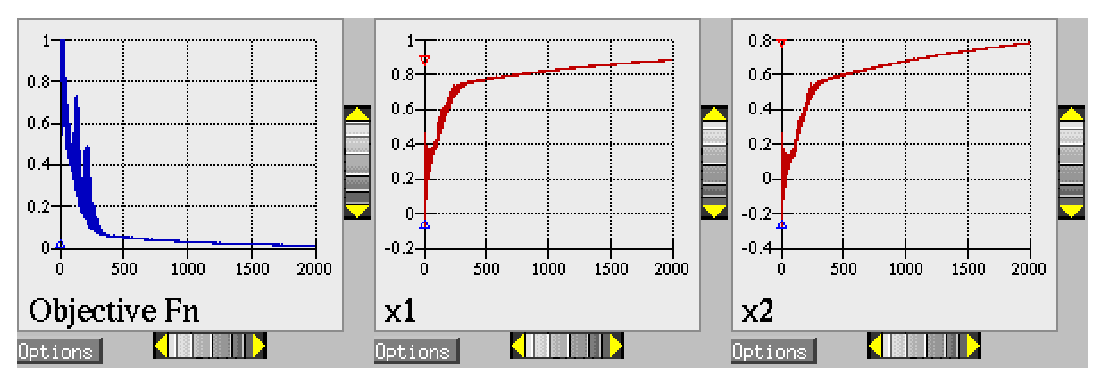
\includegraphics[width=\textwidth]{images/dak_graphics_ps_opt}}\\
  \multicolumn{2}{c}{(a)}\\
  \qquad\\
  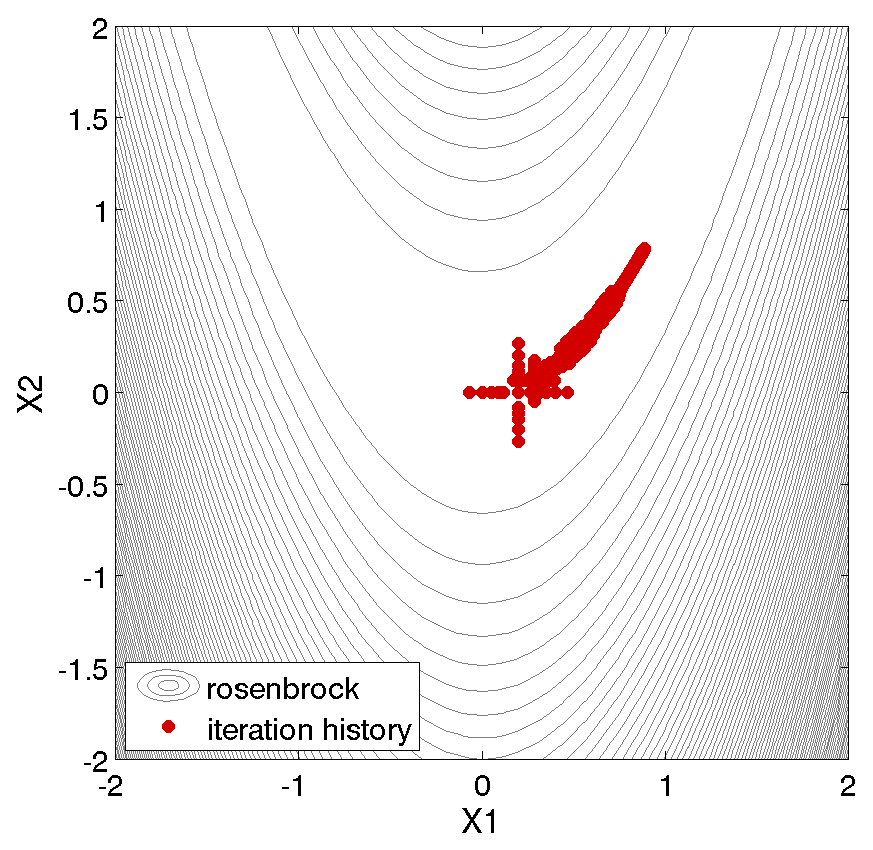
\includegraphics[height=2.5in]{images/rosen_ps_opt_pts} &
  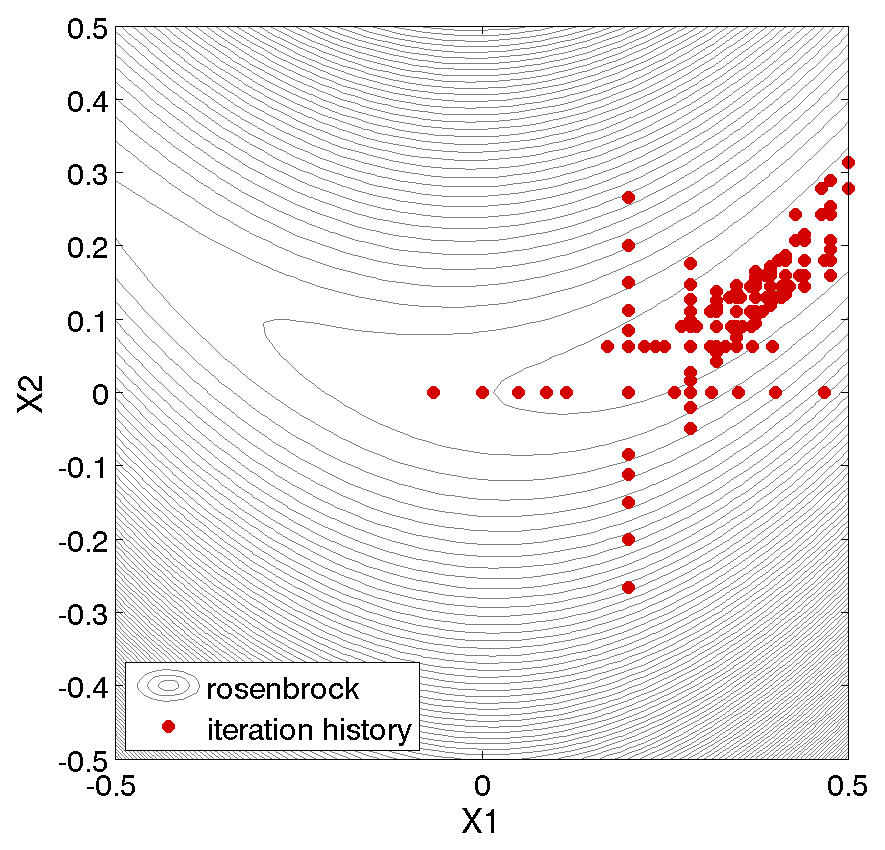
\includegraphics[height=2.5in]{images/rosen_ps_opt_pts2} \\
  (b) & (c)
  \end{tabular}
  \caption{Rosenbrock pattern search optimization example: (a) screen
    capture of the Dakota graphics, (b) sequence of design points
    (dots) evaluated and (c) close-up view illustrating the shape of
    the coordinate pattern used. }
  \label{opt:examples:ps_graphics}
\end{figure}

While pattern search algorithms are useful in many optimization
problems, this example shows some of the drawbacks to this algorithm.
While a pattern search method may make good initial progress towards
an optimum, it is often slow to converge. On a smooth, differentiable
function such as Rosenbrock's function, a nongradient-based method
will not be as efficient as a gradient-based method. However, there
are many engineering design applications where gradient information is
inaccurate or unavailable, which renders gradient-based optimizers
ineffective. Thus, pattern search algorithms (and other
nongradient-based algorithms such as genetic algorithms as discussed in the
next section) are often good choices in complex engineering applications
when the quality of gradient data is suspect.

\subsection{Nongradient-based Optimization via Evolutionary Algorithm}\label{opt:examples:ea}

In contrast to pattern search algorithms, which are local optimization
methods, evolutionary algorithms (EA) are global optimization
methods. As was described above for the pattern search algorithm, the
Rosenbrock function is not an ideal test problem for showcasing the
capabilities of evolutionary algorithms. Rather, EAs are best suited
to optimization problems that have multiple local optima, and where
gradients are either too expensive to compute or are not readily available.

Evolutionary algorithms are based on Darwin's theory of survival of
the fittest. The EA algorithm starts with a randomly selected
population of design points in the parameter space, where the values
of the design parameters form a ``genetic string,'' analogous
to DNA in a biological system, that uniquely represents each design
point in the population. The EA then follows a sequence of
generations, where the best design points in the population (i.e.,
those having low objective function values) are considered to be the
most ``fit'' and are allowed to survive and reproduce. The EA
simulates the evolutionary process by employing the mathematical
analogs of processes such as natural selection, breeding, and
mutation. Ultimately, the EA identifies a design point (or a family of
design points) that minimizes the objective function of the
optimization problem. An extensive discussion of EAs is beyond the
scope of this text, but may be found in a variety of sources (cf.,
~\cite{Haf92} pp. 149-158;~\cite{Gol89}). Currently, the EAs available
in Dakota include a genetic algorithm for problems involving discrete
variables and an evolution strategy with self-adaptation for problems
with continuous variables. Details of these algorithms are given in
the Dakota Reference Manual~\cite{RefMan}. The SCOLIB library, which
provides the EA software that has been linked into Dakota, is
described in~\cite{Har06}.

\begin{figure}[ht!]
  \centering
  \begin{bigbox}
    \begin{small}
      \verbatimtabinput[8]{dakota_rosenbrock_ea_opt.in}
    \end{small}
  \end{bigbox}
  \caption{Rosenbrock evolutionary algorithm optimization example: the
  Dakota input file.}
  \label{opt:examples:rosenbrock_ea}
\end{figure}

Figure~\ref{opt:examples:rosenbrock_ea} shows a Dakota input file that
uses an EA to minimize the Rosenbrock function. For this
example the EA has a population size of 50. At the start of the first
generation, a random number generator is used to select 50 design
points that will comprise the initial population. \emph{[A specific
  seed value is used in this example to generate repeatable results,
  although, in general, one should use the default setting which
  allows the EA to choose a random seed.]} A two-point crossover
technique is used to exchange genetic string values between the
members of the population during the EA breeding process. The result
of the breeding process is a population comprised of the 10 best
``parent'' design points (elitist strategy) plus 40 new ``child''
design points. The EA optimization process will be terminated after
either 100 iterations (generations of the EA) or 2,000 function
evaluations. The EA software available in Dakota provides the user
with much flexibility in choosing the settings used in the
optimization process. See~\cite{RefMan} and~\cite{Har06} for details on these
settings.

The following command runs Dakota on the input file:
\begin{small}
\begin{verbatim}
    dakota dakota_rosenbrock_ea_opt.in > ea_opt.out
\end{verbatim}
\end{small}

A corresponding output file named \texttt{ea\_opt.out.sav} appears in
\texttt{Dakota/examples/tutorial}. The EA optimization results
printed at the end of this file show that the best design point found
was $(x_1,x_2) = (0.98,0.95)$. The file
\texttt{ea\_tabular.dat.sav} provides a listing of the design
parameter values and objective function values for all 2,000 design
points evaluated during the running of the EA. Figure~
\ref{opt:examples:rosenbrock_ea_graphics}(a) shows the population of
50 randomly selected design points that comprise the first generation
of the EA, and Figure~\ref{opt:examples:rosenbrock_ea_graphics}(b)
shows the final population of 50 design points, where most of the 50
points are clustered near $(x_1,x_2) = (0.98,0.95)$.

\begin{figure}[hbt!]
  \centering
  \begin{tabular}{cc}
  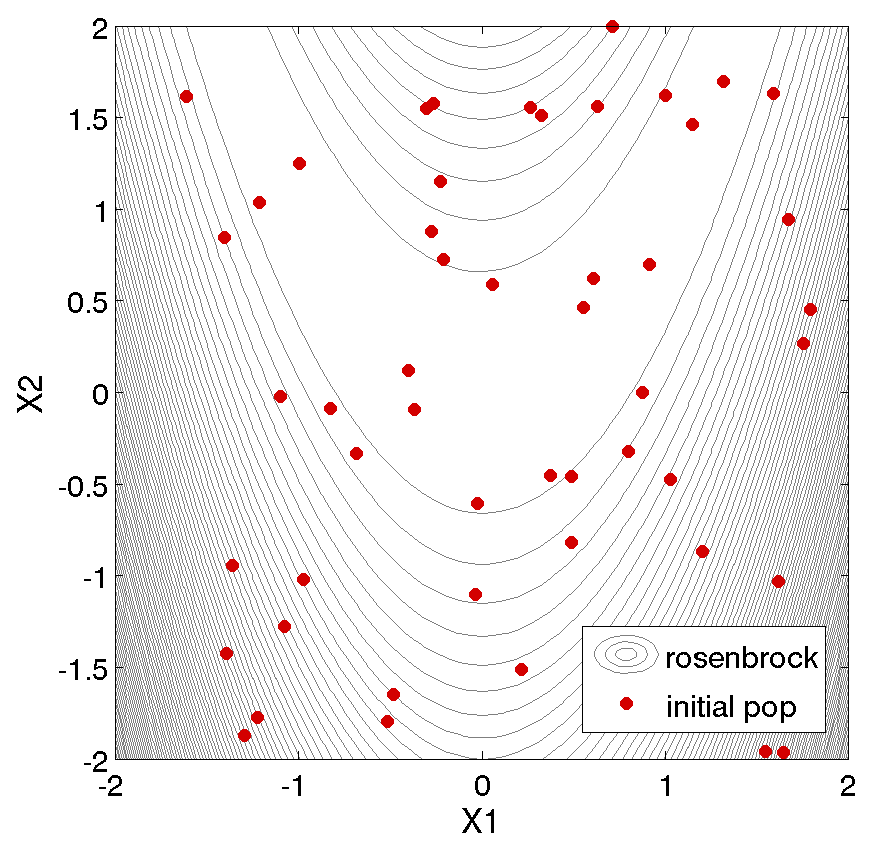
\includegraphics[height=2.5in]{images/rosen_ea_init} &
  \includegraphics[height=2.5in]{images/rosen_ea_final} \\
  (a) & (b)
  \end{tabular}
  \caption{Rosenbrock evolutionary algorithm optimization example: 50
    design points in the (a) initial and (b) final populations
    selected by the evolutionary algorithm. }
  \label{opt:examples:rosenbrock_ea_graphics}
\end{figure}

As described above, an EA is not well-suited to an optimization
problem involving a smooth, differentiable objective such as the
Rosenbrock function. Rather, EAs are better suited to optimization
problems where conventional gradient-based optimization fails, such as
situations where there are multiple local optima and/or gradients are
not available. In such cases, the computational expense of an EA is
warranted since other optimization methods are not applicable or
impractical. In many optimization problems, EAs often quickly identify
promising regions of the design space where the global minimum may be
located. However, an EA can be slow to converge to the optimum. For
this reason, it can be an effective approach to combine the global
search capabilities of a EA with the efficient local search of a
gradient-based algorithm in a \emph{hybrid optimization} strategy. In
this approach, the optimization starts by using a few iterations of a
EA to provide the initial search for a good region of the parameter
space (low objective function and/or feasible constraints), and then
it switches to a gradient-based algorithm (using the best design point
found by the EA as its starting point) to perform an efficient local
search for an optimum design point. More information on this hybrid
approach is provided in Chapter~\ref{strat}.

In addition to the evolutionary algorithm capabilities in the
\texttt{coliny\_ea} method, there is a single-objective genetic algorithm
method called \texttt{soga}.
%The major differences are that
%\texttt{soga} allows a warm start (e.g., you can read in starting
%solutions from a file), and it allows one to specify a mix of
%continuous and discrete design variables.
For more information on \texttt{soga}, see Chapter~\ref{opt}.

\chapter{Nonlinear Least Squares Capabilities}\label{nls}

\section{Overview}\label{nls:overview}

Nonlinear least-squares methods are optimization algorithms that
exploit the special structure of a sum of the squares objective
function~\cite{Gil81}. These problems commonly arise in parameter
estimation, system identification, and test/analysis reconciliation.
To exploit the problem structure, more granularity is needed
in the response data than is required for a typical optimization
problem.  That is, rather than using the sum-of-squares objective
function and its gradient, least-squares iterators require each term
used in the sum-of-squares formulation along with its gradient. This
means that the $m$ functions in the Dakota response data set consist
of the individual least-squares terms along with any nonlinear
inequality and equality constraints. These individual terms are often
called \emph{residuals} when they denote differences of
observed quantities from values computed by the model whose parameters
are being estimated.

The enhanced granularity needed for nonlinear least-squares algorithms
allows for simplified computation of an approximate Hessian matrix.
In Gauss-Newton-based methods for example, the true Hessian matrix is
approximated by neglecting terms in which residuals multiply
Hessians (matrices of second
partial derivatives) of residuals,
under the assumption that the residuals tend towards zero at
the solution. As a result, residual function value and gradient
information (first-order information) is sufficient to define the
value, gradient, and approximate Hessian of the sum-of-squares
objective function (second-order information). See
Section~\ref{introduction:background:nonlinear} for additional details
on this approximation.

In practice, least-squares solvers will tend to be significantly more
efficient than general-purpose optimization algorithms when the
Hessian approximation is a good one, e.g., when the residuals tend
towards zero at the solution. Specifically, they can exhibit the
quadratic convergence rates of full Newton methods, even though only
first-order information is used. Gauss-Newton-based least-squares
solvers may experience difficulty when the residuals at the solution
are significant.

In order to specify a least-squares problem, the responses section of
the Dakota input should be configured using
\texttt{calibration\_terms} (as opposed to
\texttt{num\_objective\_functions} in the case of optimization). 
The calibration terms refer to the residuals (e.g. typically the differences between 
the simulation model and the data).  Note that Dakota expects the residuals and 
not the square of the residuals.  Any
linear or nonlinear constraints are handled in an identical way to
that of optimization (see Section~\ref{opt:overview}; note that
neither Gauss-Newton nor NLSSOL require any constraint augmentation
and NL2SOL supports neither linear nor nonlinear constraints).
Gradients of the least-squares terms and nonlinear constraints are
required and should be specified using either
\texttt{numerical\_gradients}, \texttt{analytic\_gradients}, or
\texttt{mixed\_gradients}. Since explicit second derivatives
are not used by the least-squares methods,
the \texttt{no\_hessians} specification should be used.  Dakota's
scaling options, described in Section~\ref{opt:additional:scaling} can
be used on least-squares problems, using the
\texttt{calibration\_term\_scales} keyword to scale least-squares
residuals, if desired.

\section{Solution Techniques}\label{nls:solution}

Nonlinear least-squares problems can be solved using the Gauss-Newton
algorithm, which leverages the full Newton method from OPT++, the
NLSSOL algorithm, which is closely related to NPSOL, or the NL2SOL
algorithm, which uses a secant-based algorithm. Details for each are
provided below.

\subsection{Gauss-Newton}\label{nls:solution:gauss}

Dakota's Gauss-Newton algorithm consists of combining an
implementation of the Gauss-Newton Hessian approximation (see
Section~\ref{introduction:background:nonlinear}) with full Newton
optimization algorithms from the OPT++ package~\cite{MeOlHoWi07} (see
Section~\ref{opt:software:optpp}). This approach can be selected using
the \texttt{optpp\_g\_newton} method specification. An example
specification follows:
\begin{small}
\begin{verbatim}
    method,
          optpp_g_newton
            max_iterations = 50
            convergence_tolerance = 1e-4
            output debug
\end{verbatim}
\end{small}

Refer to the Dakota Reference Manual~\cite{RefMan} for more detail on the
input commands for the Gauss-Newton algorithm.

The Gauss-Newton algorithm is gradient-based and is best suited for
efficient navigation to a local least-squares solution in the vicinity
of the initial point. Global optima in multimodal design spaces may be
missed. Gauss-Newton supports bound, linear, and nonlinear
constraints. For the nonlinearly-constrained case, constraint Hessians
(required for full-Newton nonlinear interior point optimization
algorithms) are approximated using quasi-Newton secant updates.  Thus,
both the objective and constraint Hessians are approximated using
first-order information.

\subsection{NLSSOL}\label{nls:solution:nlssol}

The NLSSOL algorithm is a commercial software product of Stanford
University that is bundled with current versions of the NPSOL library
(see Section~\ref{opt:software:npsol}).  It uses an SQP-based approach
to solve generally-constrained nonlinear least-squares problems. It
periodically employs the Gauss-Newton Hessian approximation to
accelerate the search. Like the Gauss-Newton algorithm of
Section~\ref{nls:solution:gauss}, its derivative order is balanced in
that it requires only first-order information for the least-squares
terms and nonlinear constraints. This approach can be selected using
the \texttt{nlssol\_sqp} method specification. An example
specification follows:
\begin{small}
\begin{verbatim}
    method,
          nlssol_sqp
            convergence_tolerance = 1e-8
\end{verbatim}
\end{small}

Refer to the Dakota Reference Manual~\cite{RefMan} for more detail on the
input commands for NLSSOL.

\subsection{NL2SOL}\label{nls:solution:nl2sol}

The NL2SOL algorithm~\cite{Den81} is a secant-based least-squares
algorithm that is $q$-superlinearly convergent.  It adaptively chooses
between the Gauss-Newton Hessian approximation and this approximation
augmented by a correction term from a secant update.
NL2SOL is appropriate
for ``large residual'' problems, i.e., least-squares problems for
which the residuals do not tend towards zero at the solution.

\subsection{Additional Features and Future plans}\label{nls:solution:future}

Dakota can calculate confidence intervals on estimated parameters.
These are determined for individual parameters; they are not joint
confidence intervals.  The intervals reported are 95\% intervals
around the estimated parameters, and are calculated as the optimal
value of the estimated parameters $+/-$ a t-test statistic times the
standard error (SE) of the estimated parameter vector.  The SE is
based on a linearization approximation involving the matrix of the
derivatives of the model with respect to the derivatives of the
estimated parameters.  In the case where these gradients are extremely
inaccurate or the model is very nonlinear, the confidence intervals
reported are likely to be inaccurate as well.  Future work on
generating confidence intervals on the estimated parameters for
nonlinear least-squares methods will involve adding Bonferroni
confidence intervals and one or two methods for calculating joint
confidence intervals (such as a linear approximation and the F-test
method). See~\cite{Seb03} and~\cite{Vug07} for more details about
confidence intervals. Note that confidence intervals are not
calculated when scaling is used, when the number of least-squares
terms is less than the number of parameters to be estimated, or when
using numerical gradients.

Dakota also allows a form of weighted least squares.  The user can
specify a set of weights that are used to weight each residual term
using the keyword \texttt{calibration\_weights}.  Note that these
weights must be pre-determined by the user and entered in the Dakota
input file: they are not calculated on-the-fly.  The user can also
specify scaling for the least-squares terms.  Scaling is applied
before weighting; usually one or the other would be applied but not
both.  The Responses section in the Dakota Reference
Manual~\cite{RefMan} has more detail about weighting and scaling of
the residual terms.

The least-squares branch in Dakota is an area of continuing
enhancements, particularly through the addition of new least-squares
algorithms. One potential future addition is the orthogonal distance
regression (ODR) algorithms which estimate values for both independent
and dependent parameters.

\section{Examples}\label{nls:examples}

Both the Rosenbrock and textbook example problems can be formulated as
nonlinear least-squares problems. Refer to Chapter~\ref{additional}
for more information on these formulations.
%Figure~\ref{nls:figure01}
%shows an excerpt from output for the Rosenbrock example solved by
%the Gauss-Newton method.
%
%\begin{figure}
%\begin{bigbox}
%\begin{small}
%\begin{verbatim}
%     Active response data for function evaluation 1:
%     Active set vector = { 3 3 } Deriv vars vector = { 1 2 }
%                          -4.4000000000e+00 least_sq_term_1
%                           2.2000000000e+00 least_sq_term_2
%      [  2.4000000000e+01  1.0000000000e+01 ] least_sq_term_1 gradient
%      [ -1.0000000000e+00  0.0000000000e+00 ] least_sq_term_2 gradient
%\end{verbatim}
%\end{small}
%\end{bigbox}
%\caption{Example of intermediate output from a Gauss-Newton method.}
%\label{nls:figure01}
%\end{figure}

Figure~\ref{nls:figure02} shows an excerpt from the output 
obtained when running NL2SOL on a five-dimensional problem. 
This input file is named \texttt{dakota\_nl2test.in} found 
in the \texttt{Dakota/test} directory. 
Note that the optimal parameter estimates are printed, 
followed by the residual norm and values of the individual 
residual terms, followed by the confidence intervals on the parameters. 

\begin{figure}
\begin{bigbox}
\begin{small}
\begin{verbatim}
<<<<< Iterator nl2sol completed.
<<<<< Function evaluation summary: 27 total (26 new, 1 duplicate)
<<<<< Best parameters          =
                      3.7541004764e-01 x1
                      1.9358463401e+00 x2
                     -1.4646865611e+00 x3
                      1.2867533504e-02 x4
                      2.2122702030e-02 x5
<<<<< Best residual norm =  7.3924926090e-03; 0.5 * norm^2 =  2.7324473487e-05
<<<<< Best residual terms      =
                     -2.5698266189e-03
                      4.4759880011e-03
                      9.9223430643e-04
                     -1.0634409194e-03

...

Confidence Interval for x1 is [  3.7116510206e-01,  3.7965499323e-01 ]
Confidence Interval for x2 is [  1.4845485507e+00,  2.3871441295e+00 ]
Confidence Interval for x3 is [ -1.9189348458e+00, -1.0104382765e+00 ]
Confidence Interval for x4 is [  1.1948590669e-02,  1.3786476338e-02 ]
Confidence Interval for x5 is [  2.0289951664e-02,  2.3955452397e-02 ]

\end{verbatim}
\end{small}
\end{bigbox}
\caption{Example of confidence intervals on optimal parameters}
\label{nls:figure02}
\end{figure}

The analysis driver script (the script being driven by Dakota) 
has to perform several tasks in the case of parameter estimation 
using nonlinear least-squares methods.  The analysis driver script 
must: (1) read in the values of the parameters supplied by Dakota;
(2) run the computer simulation with these parameter values;
(3) retrieve the results from the computer simulation;
(4) compute the difference between each computed simulation value
and the corresponding experimental or measured value; and 
(5) write these residuals (differences)
to an external file that gets passed back to Dakota.  Note there 
will be one line per residual term, specified with 
\texttt{num\_least\_squares\_terms}
in the Dakota input file.   It is the last two steps which are different from 
most other Dakota applications.  

To simplify specifying a least squares problem, a user may specify a
data file containing experimental results or other calibration data.
This file may be specified with \texttt{calibration\_data\_file}. 
In this case, Dakota will calculate the residuals (that is, the
simulation model results minus the experimental results), and the
user-provided script can omit this step: the script can just return
the simulation outputs of interest.  An example of this can be found
in the file named \texttt{dakota\_nls\_datafile.in} in the
\texttt{Dakota/examples/methods} directory.  In this example, there
are 3 residual terms.  The data file of experimental results
associated with this example is \texttt{least\_squares\_test.dat}.
These three values are subtracted from the least-squares terms to
produce residuals for the nonlinear least-squares problem.
Note that the file may be annotated (specified by \texttt{annotated}) or 
freeform (specified by \texttt{freeform}). The number of experiments in the 
calibration data file may be specified with \texttt{num\_experiments}, 
with one row of data per experiment.
Finally, this data file may contain additional information than just the observed 
experimental responses.  If the observed data has measurement error associated with it, 
this can be specified in columns of such error data after the response data. 
The number of calibration terms which have associated error in the data 
set is given by \texttt{num\_std\_deviations}.  Additionally, there is sometimes the 
need to specify configuration variables.  These are often used in Bayesian calibration 
analysis.  These are specified as \texttt{num\_config\_variables}.  If the user 
specifies a positive number of configuration variables, it is expected that they will 
occur in the text file before the responses. 

%\chapter{Surrogate-Based Minimization}\label{sbm}

\section{Overview}\label{sbm:overview}

Surrogate models approximate an original, high fidelity ``truth''
model, typically at reduced computational cost.  In Dakota, several
surrogate model selections are possible, which are categorized as data
fits, multifidelity models, and reduced-order models, as described in
Section~\ref{models:surrogate}.  In the context of minimization
(optimization or calibration), surrogate models can speed convergence
by reducing function evaluation cost or smoothing noisy response
functions.  Three categories of surrogate-based minimization are
discussed in this chapter:
\begin{itemize}
\item Trust region-managed surrogate-based local minimization, with
  data fit surrogate, multifidelity models, or reduced-order models.

\item Surrogate-based global minimization, where a single surrogate is
  built (and optionally iteratively updated) over the whole design
  space.

\item Efficient global minimization: nongradient-based constrained and
  unconstrained optimization and nonlinear least squares based on
  Gaussian process models, guided by an expected improvement function.
\end{itemize}

\section{Surrogate-Based Local Minimization}\label{sbm:sblm}

In the surrogate-based local minimization method (keyword:
\texttt{surrogate\_based\_local}) the minimization algorithm operates
on a surrogate model instead of directly operating on the
computationally expensive simulation model. The surrogate model can be
based on data fits, multifidelity models, or reduced-order models, as
described in Section~\ref{models:surrogate}. Since the surrogate will
generally have a limited range of accuracy, the surrogate-based local
algorithm periodically checks the accuracy of the surrogate model
against the original simulation model and adaptively manages the
extent of the approximate optimization cycles using a trust region
approach.

%The surrogate-based local method in
%Dakota can be implemented using heuristic rules (less expensive) or
%provably-convergent rules (more expensive). The heuristic approach
%is particularly effective on real-world engineering design problems
%that contain nonsmooth features (e.g., slope discontinuities,
%numerical noise) where gradient-based optimization methods often have
%trouble, and where the computational expense of the simulation
%precludes the use of nongradient-based methods.

Refer to the Dakota Theory Manual~\cite{TheoMan} for algorithmic
details on iterate acceptance, merit function formulations,
convergence assessment, and constraint relaxation.


\subsection{SBO with Data Fits}\label{sbm:sblm:surface}

When performing SBO with local, multipoint, and global data fit
surrogates, it is necessary to regenerate or update the data fit for
each new trust region.  In the global data fit case, this can mean
performing a new design of experiments on the original high-fidelity
model for each trust region, which can effectively limit the approach
to use on problems with, at most, tens of variables.
Figure~\ref{fig:sbo_df} displays this case.  However, an important
benefit of the global sampling is that the global data fits can tame
poorly-behaved, nonsmooth, discontinuous response variations within
the original model into smooth, differentiable, easily navigated
surrogates.  This allows SBO with global data fits to extract the
relevant global design trends from noisy simulation data.

\begin{wrapfigure}{r}{.3\textwidth}
  \centering
  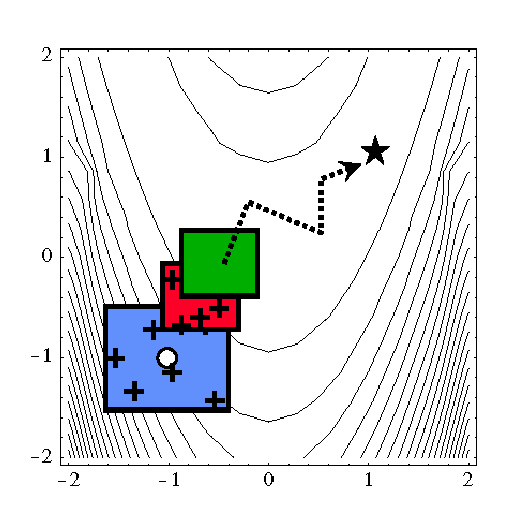
\includegraphics[width=.3\textwidth]{images/sbo_df}
  \caption{SBO iteration progression for global data fits.}
  \label{fig:sbo_df}
\end{wrapfigure}
When enforcing local consistency between a global data fit surrogate
and a high-fidelity model at a point, care must be taken to balance
this local consistency requirement with the global accuracy of the
surrogate.  In particular, performing a correction on an existing
global data fit in order to enforce local consistency can skew the
data fit and destroy its global accuracy.  One approach for achieving
this balance is to include the consistency requirement within the data
fit process by constraining the global data fit calculation (e.g.,
using constrained linear least squares).  This allows the data fit to
satisfy the consistency requirement while still addressing global
accuracy with its remaining degrees of freedom.
% Use figure from Theresa's paper?  Use equations from notes?
Embedding the consistency within the data fit also reduces the
sampling requirements.  For example, a quadratic polynomial normally
requires at least $(n+1)(n+2)/2$ samples for $n$ variables to perform
the fit.  However, with an embedded first-order consistency constraint
at a single point, the minimum number of samples is reduced by $n+1$ 
to $(n^2+n)/2$.
% With gradient information in each sample, this can be further
% reduced to ceil(n+2/2) samples.
%This corresponds to defining the terms of a symmetric Hessian matrix
%and points to an alternate approach.  Rather than enforcing
%consistency through constrained least squares, one can embed
%consistency directly by employing a Taylor series centered at the
%point of local consistency enforcement and globally estimating the
%higher order terms.  In the quadratic polynomial example, a
%second-order Taylor series with globally estimated Hessian terms
%requires the same $(n^2+n)/2$ samples and directly satisfies
%first-order consistency.  To further reduce sampling requirements in
%this case, one can choose to perform only partial updates (e.g., the
%diagonal) of the Hessian matrix~\cite{Per02}.

% Additional research area: Exploiting variance estimators to guide
% global search (e.g., kriging)

In the local and multipoint data fit cases, the iteration progression
will appear as in Fig.~\ref{fig:sbo_mh}.  Both cases involve a single
new evaluation of the original high-fidelity model per trust region,
with the distinction that multipoint approximations reuse information
from previous SBO iterates.  Like model hierarchy surrogates, these
techniques scale to larger numbers of design variables.  Unlike model
hierarchy surrogates, they generally do not require surrogate
corrections, since the matching conditions are embedded in the
surrogate form (as discussed for the global Taylor series approach
above).  The primary disadvantage to these surrogates is that the
region of accuracy tends to be smaller than for global data fits and
multifidelity surrogates, requiring more SBO cycles with smaller trust
regions.
%In SBO with surface fit functions, a sequence of optimization
%subproblems are evaluated, each of which is confined to a subset of
%the parameter space known as a ``trust region.'' Inside each trust
%region, Dakota's data sampling methods are used to evaluate the
%response quantities at a small number (order $10^{1}$ to $10^{2}$) of
%design points. Next, multidimensional surface fitting is performed to
%create a surrogate function for each of the response quantities.
%Finally, optimization is performed using the surrogate functions in
%lieu of the actual response quantities, and the optimizer's search is
%limited to the region inside the trust region bounds. A validation
%procedure is then applied to compare the predicted improvement in the
%response quantities to the actual improvement in the response
%quantities. Based on the results of this validation, the optimum
%design point is either accepted or rejected and the size of the trust
%region is either expanded, contracted, or left unchanged. The sequence
%of optimization subproblems continues until the SBO strategy
%convergence criteria are satisfied
More information on the design of experiments methods is available in
Chapter~\ref{dace}, and the data fit surrogates are described in
Section~\ref{models:surrogate:datafit}.

Figure~\ref{sbm:sblm_rosen} shows a Dakota input file that implements
surrogate-based optimization on Rosenbrock's function. This input file
is named \texttt{dakota\_sbo\_rosen.in} in the \texttt{Dakota/test}
directory.  The first method keyword block contains the SBO 
keyword \texttt{surrogate\_based\_local}, plus the commands for
specifying the trust region size and scaling factors. The optimization
portion of SBO, using the CONMIN Fletcher-Reeves conjugate gradient method,
is specified in the following keyword blocks for
\texttt{method}, \texttt{model}, \texttt{variables}, and
\texttt{responses}.  The model used by the optimization method 
specifies that a global surrogate will be used to map variables into
responses (no \texttt{interface} specification is used by the
surrogate model). The global surrogate is constructed using a DACE
method which is identified with the \texttt{`SAMPLING'} identifier.
This data sampling portion of SBO is specified in the final set of
keyword blocks for \texttt{method}, \texttt{model},
\texttt{interface}, and \texttt{responses} (the earlier 
\texttt{variables} specification is reused). This example problem uses 
the Latin hypercube sampling method in the LHS software to select 10
design points in each trust region. A single surrogate model is
constructed for the objective function using a quadratic polynomial.
The initial trust region is centered at the design point
$(x_1,x_2)=(-1.2,1.0)$, and extends $\pm 0.4$ (10\% of the global
bounds) from this point in the $x_1$ and $x_2$ coordinate directions.
\begin{figure}
  \begin{bigbox}
    \begin{tiny}
      \verbatimtabinput[8]{dakota_sbo_rosen.in}
    \end{tiny}
  \end{bigbox}
  \caption{Dakota input file for the surrogate-based local optimization
    example.}
  \label{sbm:sblm_rosen}
\end{figure}

If this input file is executed in Dakota, it will converge to the
optimal design point at $(x_{1},x_{2})=(1,1)$ in approximately 800
function evaluations. While this solution is correct, it is obtained
at a much higher cost than a traditional gradient-based optimizer
(e.g., see the results obtained from \texttt{dakota\_rosenbrock.in}).
This demonstrates that the SBO method with global data fits is not
really intended for use with smooth continuous optimization problems;
direct gradient-based optimization can be more efficient for such
applications. Rather, SBO with global data fits is best-suited for the
types of problems that occur in engineering design where the response
quantities may be discontinuous, nonsmooth, or may have multiple local
optima~\cite{Giu02}. In these types of engineering design problems,
traditional gradient-based optimizers often are ineffective, whereas
global data fits can extract the global trends of interest despite the
presence of local nonsmoothness (for an example problem with multiple
local optima, look in \texttt{Dakota/test} for the file
\texttt{dakota\_sbo\_sine\_fcn.in}~\cite{Giu00}).

The surrogate-based local minimizer is only mathematically
guaranteed to find a local minimum. However, in practice, SBO can often find 
the global minimum.  Due to the random sampling method used within the
SBO algorithm, the SBO method will solve a given problem a little differently 
each time it is run (unless the user specifies a particular random
number seed in the dakota input file as is shown in Figure~\ref{sbm:sblm_rosen}). 
Our experience on the quasi-sine function mentioned above is that if 
you run this problem 10 times with the same starting conditions but different 
seeds, then you will find the global minimum in about 70-80\% of the trials.
This is good performance for what is mathematically only a local optimization method.

\subsection{SBO with Multifidelity Models}\label{sbm:sblm:multifidelity}

When performing SBO with model hierarchies, the low-fidelity model is
normally fixed, requiring only a single high-fidelity evaluation to
compute a new correction for each new trust region.
Figure~\ref{fig:sbo_mh} displays this case.  This renders the
multifidelity SBO technique more scalable to larger numbers of design
variables since the number of high-fidelity evaluations per iteration
(assuming no finite differencing for derivatives) is independent of
the scale of the design problem.  However, the ability to smooth
poorly-behaved response variations in the high-fidelity model is lost,
and the technique becomes dependent on having a well-behaved
low-fidelity model\footnote{It is also possible to use a hybrid data
fit/multifidelity approach in which a smooth data fit of a noisy low
fidelity model is used in combination with a high fidelity model}.  In
addition, the parameterizations for the low and high-fidelity models
may differ, requiring the use of a mapping between these
parameterizations.  Space mapping, corrected space mapping, POD
mapping, and hybrid POD space mapping are being explored for this
purpose~\cite{Rob06a,Rob06b}.

\begin{wrapfigure}{r}{.3\textwidth}
  \centering
  \includegraphics[width=.3\textwidth]{images/sbo_mh}
  \caption{SBO iteration progression for model hierarchies.}
  \label{fig:sbo_mh}
\end{wrapfigure}
%\begin{figure}
%\epsfxsize 3in
%\centerline{\epsfbox{sbo_mh.eps}}
%\caption{SBO iteration progression for model hierarchies.}
%\label{fig:sbo_mh}
%\end{figure}

When applying corrections to the low-fidelity model, there is no
concern for balancing global accuracy with the local consistency
requirements.  However, with only a single high-fidelity model evaluation
at the center of each trust region, it is critical to use the best
correction possible on the low-fidelity model in order to achieve
rapid convergence rates to the optimum of the high-fidelity
model~\cite{Eld04}.

%SBO can also be applied with multifidelity, or hierarchical, models,
%i.e., where one has available both a high-fidelity computational model
%and a low-fidelity computational model. This situation can occur when
%the low-fidelity model neglects some physical phenomena (e.g.,
%viscosity, heat transfer, etc.) that are included in the high-fidelity
%model, or when the low-fidelity model has a lower resolution
%computational mesh than the high-fidelity model. In many cases, the
%low-fidelity model can serve as a surrogate for the high-fidelity
%model during the optimization process. Thus, the low-fidelity model
%can be used in SBO in a manner similar to the use of surface fit
%models described in Section~\ref{sbm:sblm:surface}. A key difference
%in SBO with hierarchical surrogates is that a design of experiments
%using the high-fidelity model is not required; rather high-fidelity
%evaluations are only needed at the center of the current trust-region
%and the predicted optimum point in order to correct the low-fidelity
%model and verify improvement, respectively. Another difference is that
%one of the four types of correction described in
%Section~\ref{sbm:sblm:surface} is required for SBO with multifidelity
%models.

A multifidelity test problem named
\texttt{dakota\_sbo\_hierarchical.in} is available in
\texttt{Dakota/test} to demonstrate this SBO approach. This test
problem uses the Rosenbrock function as the high fidelity model and a
function named ``lf\_rosenbrock'' as the low fidelity model. Here,
lf\_rosenbrock is a variant of the Rosenbrock function (see
\texttt{Dakota/test/lf\_rosenbrock.C} for formulation) with the
minimum point at $(x_1,x_2)=(0.80,0.44)$, whereas the minimum of the
original Rosenbrock function is $(x_1,x_2)=(1,1)$. Multifidelity SBO
locates the high-fidelity minimum in 11 high fidelity evaluations for
additive second-order corrections and in 208 high fidelity evaluations
for additive first-order corrections, but fails for zeroth-order
additive corrections by converging to the low-fidelity minimum.

\subsection{SBO with Reduced Order Models}\label{sbm:sblm:rom}

When performing SBO with reduced-order models (ROMs), the ROM is
mathematically generated from the high-fidelity model.  A critical
issue in this ROM generation is the ability to capture the effect of
parametric changes within the ROM.  Two approaches to parametric ROM
are extended ROM (E-ROM) and spanning ROM (S-ROM)
techniques~\cite{Wei06}.  Closely related techniques include tensor
singular value decomposition (SVD) methods~\cite{Lat00}.  In the
single-point and multipoint E-ROM cases, the SBO iteration can appear
as in Fig.~\ref{fig:sbo_mh}, whereas in the S-ROM, global E-ROM, and
tensor SVD cases, the SBO iteration will appear as in
Fig.~\ref{fig:sbo_df}.  In addition to the high-fidelity model
analysis requirements, procedures for updating the system matrices and
basis vectors are also required.

Relative to data fits and multifidelity models, ROMs have some
attractive advantages.  Compared to data fits such as regression-based
polynomial models, they are more physics-based and would be expected
to be more predictive (e.g., in extrapolating away from the immediate
data).  Compared to multifidelity models, ROMS may be more practical
in that they do not require multiple computational models or meshes
which are not always available.  The primary disadvantage is potential
invasiveness to the simulation code for projecting the system using
the reduced basis.


\section{Surrogate-Based Global Minimization}\label{sbm:sbgm}

Surrogate-based global minimization differs from the surrogate-based
local minimization approach discussed in the previous section in
several ways: it is not a trust-region approach; initially there is
one global surrogate constructed over a set of sample points and the
optimizer operates on that surrogate (as opposed to adaptively
selecting points and re-building a surrogate in each trust region);
and there is no guarantee of convergence.

The \texttt{surrogate\_based\_global} method was developed to address
two needs.  The first is the case where a user wishes to use existing
function evaluations or a fixed sample size (perhaps based on
computational cost and allocation of resources) to build a surrogate
once and optimize on it.  In this case (a single global optimization
on a surrogate model), the set of surrogate building points is
determined in advance as opposed to the trust-region local surrogate
optimization in which the number of ``true'' function evaluations
depends on the location and size of the trust region, the goodness of
the surrogate within the trust-region, and problem characteristics.

In the second \texttt{surrogate\_based\_global} use case, we want to
update the surrogate, but globally.  That is, we add points to the
sample set used to create the surrogate, rebuild the surrogate, and
then perform another global optimization on the new surrogate.  Thus,
surrogate-based global optimization can be used in an iterative
scheme.  In one iteration, minimizers of the surrogate model are
found, and a selected subset of these are passed to the next
iteration.  In the next iteration, these surrogate points are
evaluated with the ``truth'' model, and then added to the set of
points upon which the next surrogate is constructed.  This presents a
more accurate surrogate to the minimizer at each subsequent iteration,
presumably driving to optimality quickly.  Note that a global
surrogate is constructed using the same bounds in each iteration.
This approach has no guarantee of convergence.

The surrogate-based global method was originally designed for MOGA (a
multi-objective genetic algorithm).  Since genetic algorithms often
need thousands or tens of thousands of points to produce optimal or
near-optimal solutions, surrogates can help by reducing the necessary
truth model evaluations.  Instead of creating one set of surrogates
for the individual objectives and running the optimization algorithm
on the surrogate once, the idea is to select points along the
(surrogate) Pareto frontier, which can be used to supplement the
existing points.  In this way, one does not need to use many points
initially to get a very accurate surrogate.  The surrogate becomes
more accurate as the iterations progress.

Most single objective optimization methods will return only a single
optimal point.  In that case, only one point from the surrogate model
will be evaluated with the ``true'' function and added to the pointset
upon which the surrogate is based.  In this case, it will take many
iterations of the surrogate-based global optimization for the approach
to converge, and its utility may not be as great as for the
multi-objective case when multiple optimal solutions are passed from
one iteration to the next to supplement the surrogate.  Note that the
user has the option of appending the optimal points from the surrogate
model to the current set of truth points or using the optimal points
from the surrogate model to replace the optimal set of points from the
previous iteration.  Although appending to the set is the default
behavior, at this time we strongly recommend using the option
\texttt{replace\_points} because it appears to be more accurate and
robust.

When using the surrogate-based global method, we first recommend
running one optimization on a single surrogate model. That is, set
\texttt{max\_iterations} to 1.  This will allow one to get a sense of
where the optima are located and also what surrogate types are the
most accurate to use for the problem.  Note that by fixing the seed of
the sample on which the surrogate is built, one can take a Dakota
input file, change the surrogate type, and re-run the problem without
any additional function evaluations by specifying the use of the
dakota restart file which will pick up the existing function
evaluations, create the new surrogate type, and run the optimization
on that new surrogate.  Also note that one can specify that surrogates
be built for all primary functions and constraints or for only a
subset of these functions and constraints.  This allows one to use a
"truth" model directly for some of the response functions, perhaps due
to them being much less expensive than other functions.  Finally, a
diagnostic threshold can be used to stop the method if the surrogate
is so poor that it is unlikely to provide useful points.  If the
goodness-of-fit has an R-squared value less than 0.5, meaning that
less than half the variance of the output can be explained or
accounted for by the surrogate model, the surrogate-based global
optimization stops and outputs an error message.  This is an arbitrary
threshold, but generally one would want to have an R-squared value as
close to 1.0 as possible, and an R-squared value below 0.5 indicates a
very poor fit.

For the surrogate-based global method, we initially recommend a small
number of maximum iterations, such as 3--5, to get a sense of how the
optimization is evolving as the surrogate gets updated globally.  If
it appears to be changing significantly, then a larger number (used in
combination with restart) may be needed.

Figure~\ref{sbm:sbgm_moga} shows a Dakota input file that implements
surrogate-based global optimization on a multi-objective test function. 
This input file
is named \texttt{dakota\_su\_mogatest1.in} in the \texttt{Dakota/test}
directory.  The first method keyword block contains the
keyword \texttt{surrogate\_based\_global}, plus the commands for
specifying five as the maximum iterations and the option to replace 
points in the global surrogate construction. The method block identified 
as MOGA specifies a multi-objective genetic algorithm optimizer and its 
controls.  The model keyword block specifies a surrogate model.  
In this case, a \texttt{gaussian\_process} model is used as a surrogate. 
The \texttt{dace\_method\_pointer} specifies that the surrogate will be 
build on 100 Latin Hypercube samples with a seed = 531.
The remainder of the input specification deals with the interface 
to the actual analysis driver and the 2 responses being returned 
as objective functions from that driver. 

\begin{figure}
  \begin{bigbox}
    \begin{tiny}
      \verbatimtabinput[8]{dakota_su_mogatest1.in}
    \end{tiny}
  \end{bigbox}
  \caption{Dakota input file for the surrogate-based global optimization
    example.}
  \label{sbm:sbgm_moga}
\end{figure}
 
\section{Efficient Global Minimization}\label{sbm:egm}

Efficient Global Optimization (EGO) is a global optimization technique
that employs response surface surrogates~\cite{Jon98,Hua06}.  In each
EGO iteration, a Gaussian process (GP) approximation for the objective
function is constructed based on sample points of the true simulation.
The GP allows one to specify the prediction at a new input location as
well as the uncertainty associated with that prediction.  The key idea
in EGO is to maximize an Expected Improvement Function (EIF), defined
as the expectation that any point in the search space will provide a
better solution than the current best solution, based on the expected
values and variances predicted by the GP model.  It is important to
understand how the use of this EIF leads to optimal solutions.  The
EIF indicates how much the objective function value at a new potential
location is expected to be less than the predicted value at the
current best solution.  Because the GP model provides a Gaussian
distribution at each predicted point, expectations can be calculated.
Points with good expected values and even a small variance will have a
significant expectation of producing a better solution (exploitation),
but so will points that have relatively poor expected values and
greater variance (exploration).  The EIF incorporates both the idea of
choosing points which minimize the objective and choosing points about
which there is large prediction uncertainty (e.g., there are few or no
samples in that area of the space, and thus the probability may be
high that a sample value is potentially lower than other values).
Because the uncertainty is higher in regions of the design space with
few observations, this provides a balance between exploiting areas of
the design space that predict good solutions, and exploring areas
where more information is needed.

There are two major differences between our implementation and that of
~\cite{Jon98}: we do not use a branch and bound method to find points
which maximize the EIF.  Rather, we use the DIRECT algorithm.  Second,
we allow for multiobjective optimization and nonlinear least squares
including general nonlinear constraints.  Constraints are handled
through an augmented Lagrangian merit function approach (see
Surrogate-Based Minimization chapter in Dakota Theory
Manual~\cite{TheoMan}).

The method is specified as \texttt{efficient\_global}.  Currently we
do not expose any specification controls for the underlying Gaussian
process model used or for the optimization of the expected improvement
function, which is currently performed by the NCSU DIRECT
algorithm. The only item the user can specify is a seed which is 
used in the Latin Hypercube Sampling to generate the initial 
set of points which is used to construct the initial Gaussian process. 
An example specification for the EGO algorithm is shown in
Figure~\ref{sbm:egm_rosen}.  This can be found in the 
\texttt{dakota\_rosenbrock\_ego.in} file in the 
\texttt{Dakota/test} directory.
\begin{figure}
  \begin{bigbox}
    \begin{small}
      \verbatimtabinput[8]{dakota_rosenbrock_ego.in}
    \end{small}
  \end{bigbox}
  \caption{Dakota input file for the efficient global optimization example.}
  \label{sbm:egm_rosen}
\end{figure}

 % moved to Users_Advanced_Methods
\chapter{Models}\label{models}

\section{Overview}\label{models:overview}

Chapters~\ref{ps} through~\ref{nls} have presented the different
``iterators'' available in DAKOTA.  An iterator iterates on a model in
order to map a set of variables into a set of responses.  This model
may involve a simple mapping involving a single interface, or it may
involve recursions using sub-iterator and sub-models.  These recursion
capabilities were developed in order to provide mechanisms for
``nesting,'' ``layering,'' and ``recasting'' of software components,
which allows the use of these components as building blocks to
accomplish more sophisticated studies, such as surrogate-based
optimization or optimization under uncertainty.  In a nested
relationship, a sub-iterator is executed using its sub-model for every
evaluation of the nested model.  In a layered relationship, on the
other hand, sub-iterators and sub-models are used only for periodic
updates and verifications.  And in a recast relationship, the input
variable and output response definitions in a sub-model are
reformulated in order to support new problem definitions.  In each of
these cases, the sub-model is of arbitrary type, such that model
recursions can be chained together in as long of a sequence as needed
(e.g., layered containing nested contained layered containing single
in Section~\ref{models:ex:ouu:sb}).  Figure~\ref{model:hier} displays
the model class hierarchy from the DAKOTA Developers
Manual~\cite{DevMan}, with derived classes for single models, nested
models, recast models, and two types of surrogate models: data fit and
hierarchical/multifidelity.  A third type of derived surrogate model
supporting reduced-order models (ROM) is planned for future releases.

\begin{figure}
  \centering 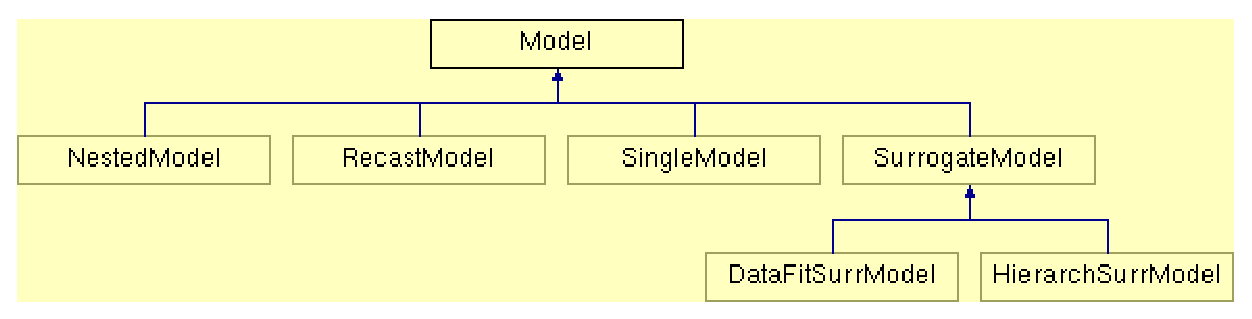
\includegraphics[scale=0.65]{images/classDakota_1_1Model}
  \caption{The DAKOTA model class hierarchy.}  \label{model:hier}
\end{figure}

Section~\ref{models:single} describes single models;
Section~\ref{models:recast} describes recast models;
Section~\ref{models:surrogate} describes surrogate models of the data
fit, multifidelity, and ROM type; and Section~\ref{models:nested}
describes nested models.  Finally, Section~\ref{models:ex} presents
a number of advanced examples demonstrating model recursion.

\section{Single Models}\label{models:single}

The single model is the simplest model type.  It uses a single
interface instance (see Chapter~\ref{interfaces}) to map variables
(see Chapter~\ref{variables}) into responses (see
Chapter~\ref{responses}).  There is no recursion in this case.  Refer
to the Models chapter in the DAKOTA Reference Manual~\cite{RefMan} for
additional information on the single model specification.

\section{Recast Models}\label{models:recast}

The recast model is not directly visible to the user within the input
specification.  Rather, it is used ``behind the scenes'' to recast the
inputs and outputs of a sub-model for the purposes of reformulating
the problem posed to an iterator.  Examples include variable and
response scaling (see Section~\ref{opt:additional:scaling}),
transformations of uncertain variables and associated response
derivatives to employ standardized random variables (see
Sections~\ref{uq:reliability:mpp} and~\ref{uq:expansion:pce}),
multiobjective optimization (see
Section~\ref{opt:additional:multiobjective}), merit functions (see
Section~\ref{sbm:sblm}), and expected improvement/feasibility (see
Sections~\ref{sbm:egm} and~\ref{uq:reliability:global}).  Refer to the
DAKOTA Developers Manual~\cite{DevMan} for additional details on the
mechanics of recasting problem formulations.

\section{Surrogate Models}\label{models:surrogate}

Surrogate models provide an approximation to an original, high
fidelity ``truth'' model.  A number of surrogate model selections are
possible, which are categorized as data fits, multifidelity models,
and reduced-order models.

Each of the surrogate model types supports the use of correction
factors that improve the local accuracy of the surrogate models. The
correction factors force the surrogate models to match the true
function values and possibly true function derivatives at the center
point of each trust region. Currently, DAKOTA supports either zeroth-,
first-, or second-order accurate correction methods, each of which can
be applied using either an additive, multiplicative, or combined
correction function. For each of these correction approaches, the
correction is applied to the surrogate model and the corrected model
is then interfaced with whatever algorithm is being employed.  The
default behavior is that no correction factor is applied.

The simplest correction approaches are those that enforce consistency
in function values between the surrogate and original models at a
single point in parameter space through use of a simple scalar offset
or scaling applied to the surrogate model.  First-order corrections
such as the first-order multiplicative correction (also known as beta
correction~\cite{Cha93}) and the first-order additive
correction~\cite{Lew00} also enforce consistency in the gradients and
provide a much more substantial correction capability that is
sufficient for ensuring provable convergence in SBO algorithms (see
Section~\ref{sbm:sblm}).  SBO convergence rates can be further
accelerated through the use of second-order corrections which also
enforce consistency in the Hessians~\cite{Eld04}, where the
second-order information may involve analytic, finite-difference, or
quasi-Newton Hessians.

Correcting surrogate models with additive corrections involves
\begin{equation}
\hat{f_{hi_{\alpha}}}({\bf x}) = f_{lo}({\bf x}) + \alpha({\bf x}) 
\label{eq:correct_val_add}
\end{equation}
where multifidelity notation has been adopted for clarity.  For
multiplicative approaches, corrections take the form
\begin{equation}
\hat{f_{hi_{\beta}}}({\bf x}) = f_{lo}({\bf x}) \beta({\bf x})
\label{eq:correct_val_mult}
\end{equation}
where, for local corrections, $\alpha({\bf x})$ and $\beta({\bf x})$
are first or second-order Taylor series approximations to the exact
correction functions:
\begin{eqnarray}
\alpha({\bf x}) & = & A({\bf x_c}) + \nabla A({\bf x_c})^T 
({\bf x} - {\bf x_c}) + \frac{1}{2} ({\bf x} - {\bf x_c})^T 
\nabla^2 A({\bf x_c}) ({\bf x} - {\bf x_c}) \label{eq:taylor_a} \\
\beta({\bf x})  & = & B({\bf x_c}) + \nabla B({\bf x_c})^T 
({\bf x} - {\bf x_c}) + \frac{1}{2} ({\bf x} - {\bf x_c})^T \nabla^2 
B({\bf x_c}) ({\bf x} - {\bf x_c}) \label{eq:taylor_b}
\end{eqnarray}
where the exact correction functions are
\begin{eqnarray}
A({\bf x}) & = & f_{hi}({\bf x}) - f_{lo}({\bf x})       \label{eq:exact_A} \\
B({\bf x}) & = & \frac{f_{hi}({\bf x})}{f_{lo}({\bf x})} \label{eq:exact_B}
\end{eqnarray}
Refer to \cite{Eld04} for additional details on the derivations.

A combination of additive and multiplicative corrections can provide
for additional flexibility in minimizing the impact of the correction
away from the trust region center.  In other words, both additive and
multiplicative corrections can satisfy local consistency, but through
the combination, global accuracy can be addressed as well.  This
involves a convex combination of the additive and multiplicative
corrections:
\begin{equation}
\hat{f_{hi_{\gamma}}}({\bf x}) = \gamma \hat{f_{hi_{\alpha}}}({\bf x}) +
(1 - \gamma) \hat{f_{hi_{\beta}}}({\bf x}) \label{eq:combined_form}
\end{equation}
where $\gamma$ is calculated to satisfy an additional matching
condition, such as matching values at the previous design iterate.

%It should be noted that in both first order correction methods, the
%function $\hat{f}(x)$ matches the function value and gradients of
%$f_{t}(x)$ at $x=x_{c}$. This property is necessary in proving that
%the first order-corrected SBO algorithms are provably convergent to a
%local minimum of $f_{t}(x)$.  However, the first order correction
%methods are significantly more expensive than the zeroth order
%correction methods, since the first order methods require computing
%both $\nabla f_{t}(x_{c})$ and $\nabla f_{s}(x_{c})$.  When the SBO
%strategy is used with either of the zeroth order correction methods,
%or with no correction method, convergence is not guaranteed to a local
%minimum of $f_{t}(x)$. That is, the SBO strategy becomes a heuristic
%optimization algorithm. From a mathematical point of view this is
%undesirable, but as a practical matter, the heuristic variants of SBO
%are often effective in finding local minima.

%\emph{Usage guidelines:}
%\begin{itemize}
%\item Both the \texttt{additive zeroth\_order} and
%  \texttt{multiplicative zeroth\_order} correction methods are
%  ``free'' since they use values of $f_{t}(x_{c})$ that are normally
%  computed by the SBO strategy.
%
%\item The use of either the \texttt{additive first\_order} method or
%  the \texttt{multiplicative first\_order} method does not necessarily
%  improve the rate of convergence of the SBO algorithm.
%
%\item When using the first order correction methods, the
%  \texttt{TRUE\_FCN\_GRAD} response keywords must be modified (see
%  bottom of Figure~\ref{sbm:sblm_rosen}) to allow either analytic or
%  numerical gradients to be computed. This provides the gradient data
%  needed to compute the correction function.
%
%\item For many computationally expensive engineering optimization
%  problems, gradients often are too expensive to obtain or are
%  discontinuous (or may not exist at all). In such cases the heuristic
%  SBO algorithm has been an effective approach at identifying optimal
%  designs~\cite{Giu02}.
%\end{itemize}

\subsection{Data Fit Surrogate Models}\label{models:surrogate:datafit}

A surrogate of the {\em data fit} type is a non-physics-based
approximation typically involving interpolation or regression of a set
of data generated from the original model.  Data fit surrogates can be
further characterized by the number of data points used in the fit,
where a local approximation (e.g., first or second-order Taylor
series) uses data from a single point, a multipoint approximation
(e.g., two-point exponential approximations (TPEA) or two-point
adaptive nonlinearity approximations (TANA)) uses a small number of
data points often drawn from the previous iterates of a particular
algorithm, and a global approximation (e.g., polynomial response
surfaces, kriging, neural networks, radial basis functions, splines)
uses a set of data points distributed over the domain of interest,
often generated using a design of computer experiments.

DAKOTA contains several types of surface fitting methods that can be
used with optimization and uncertainty quantification methods and
strategies such as surrogate-based optimization and optimization under
uncertainty. These are: polynomial models (linear, quadratic, and
cubic), first-order Taylor series expansion, kriging spatial
interpolation, artificial neural networks, multivariate adaptive
regression splines, radial basis functions, and moving least squares. 
With the exception of Taylor series methods, all of the above methods 
listed in the previous sentence are accessed in DAKOTA through the 
Surfpack library.  All of these surface fitting methods can be
applied to problems having an arbitrary number of design parameters.
However, surface fitting methods usually are practical only for
problems where there are a small number of parameters (e.g., a maximum
of somewhere in the range of 30-50 design parameters). The
mathematical models created by surface fitting methods have a variety
of names in the engineering community. These include surrogate models,
meta-models, approximation models, and response surfaces. For this
manual, the terms surface fit model and surrogate model are used.

The data fitting methods in DAKOTA include software developed by
Sandia researchers and by various researchers in the academic
community.

\subsubsection{Procedures for Surface Fitting}\label{models:surf:procedures}

The surface fitting process consists of three steps: (1) selection of
a set of design points, (2) evaluation of the true response quantities
(e.g., from a user-supplied simulation code) at these design points,
and (3) using the response data to solve for the unknown coefficients
(e.g., polynomial coefficients, neural network weights, kriging
correlation factors) in the surface fit model. In cases where there is
more than one response quantity (e.g., an objective function plus one
or more constraints), then a separate surface is built for each
response quantity. Currently, the surface fit models are built using
only 0$^{\mathrm{th}}$-order information (function values only), although
extensions to using higher-order information (gradients and Hessians)
are possible. Each surface fitting method employs a different
numerical method for computing its internal coefficients. For example,
the polynomial surface uses a least-squares approach that employs a
singular value decomposition to compute the polynomial coefficients,
whereas the kriging surface uses Maximum Likelihood Estimation to
compute its correlation coefficients. More information on the
numerical methods used in the surface fitting codes is provided in the
DAKOTA Developers Manual~\cite{DevMan}.

The set of design points that is used to construct a surface fit model
is generated using either the DDACE software package~\cite{TonXX} or the
LHS software package~\cite{Ima84}. These packages provide a variety of
sampling methods including Monte Carlo (random) sampling, Latin
hypercube sampling, orthogonal array sampling, central composite
design sampling, and Box-Behnken sampling. More information on these
software packages is provided in Chapter~\ref{dace}.

\subsubsection{Taylor Series}\label{models:surf:taylor}

The Taylor series model is purely a local approximation method. That
is, it provides local trends in the vicinity of a single point in
parameter space. The first-order Taylor series expansion is:
\begin{equation}
\hat{f}({\bf x}) \approx f({\bf x}_0) + \nabla_{\bf x} f({\bf x}_0)^T 
({\bf x} - {\bf x}_0) \label{eq:taylor1}
\end{equation}
and the second-order expansion is:
\begin{equation}
\hat{f}({\bf x}) \approx f({\bf x}_0) + \nabla_{\bf x} f({\bf x}_0)^T 
({\bf x} - {\bf x}_0) + \frac{1}{2} ({\bf x} - {\bf x}_0)^T 
\nabla^2_{\bf x} f({\bf x}_0) ({\bf x} - {\bf x}_0) \label{eq:taylor2}
\end{equation}

where ${\bf x}_0$ is the expansion point in $n$-dimensional parameter
space and $f({\bf x}_0)$, $\nabla_{\bf x} f({\bf x}_0)$, and
$\nabla^2_{\bf x} f({\bf x}_0)$ are the computed response value,
gradient, and Hessian at the expansion point, respectively.  As
dictated by the responses specification used in building the local
surrogate, the gradient may be analytic or numerical and the Hessian
may be analytic, numerical, or based on quasi-Newton secant updates.

In general, the Taylor series model is accurate only in the region of
parameter space that is close to ${\bf x}_0$ . While the accuracy is
limited, the first-order Taylor series model reproduces the correct
value and gradient at the point $\mathbf{x}_{0}$, and the second-order
Taylor series model reproduces the correct value, gradient, and
Hessian. This consistency is useful in provably-convergent
surrogate-based optimization. The other surface fitting methods do not
use gradient information directly in their models, and these methods
rely on an external correction procedure in order to satisfy the
consistency requirements of provably-convergent SBO.

\subsubsection{Two Point Adaptive Nonlinearity Approximation}\label{models:surf:tana}

The TANA-3 method~\cite{Xu98} is a multipoint approximation method
based on the two point exponential approximation~\cite{Fad90}. This
approach involves a Taylor series approximation in intermediate
variables where the powers used for the intermediate variables are
selected to match information at the current and previous expansion
points.  The form of the TANA model is:

\begin{equation}
\hat{f}({\bf x}) \approx f({\bf x}_2) + \sum_{i=1}^n 
\frac{\partial f}{\partial x_i}({\bf x}_2) \frac{x_{i,2}^{1-p_i}}{p_i} 
(x_i^{p_i} - x_{i,2}^{p_i}) + \frac{1}{2} \epsilon({\bf x}) \sum_{i=1}^n 
(x_i^{p_i} - x_{i,2}^{p_i})^2 \label{eq:tana_f}
\end{equation}

where $n$ is the number of variables and:

\begin{eqnarray}
p_i & = & 1 + \ln \left[ \frac{\frac{\partial f}{\partial x_i}({\bf x}_1)}
{\frac{\partial f}{\partial x_i}({\bf x}_2)} \right] \left/ 
\ln \left[ \frac{x_{i,1}}{x_{i,2}} \right] \right. \label{eq:tana_pi} \\
\epsilon({\bf x}) & = & \frac{H}{\sum_{i=1}^n (x_i^{p_i} - x_{i,1}^{p_i})^2 + 
\sum_{i=1}^n (x_i^{p_i} - x_{i,2}^{p_i})^2} \label{eq:tana_eps} \\
H & = & 2 \left[ f({\bf x}_1) - f({\bf x}_2) - \sum_{i=1}^n 
\frac{\partial f}{\partial x_i}({\bf x}_2) \frac{x_{i,2}^{1-p_i}}{p_i} 
(x_{i,1}^{p_i} - x_{i,2}^{p_i}) \right] \label{eq:tana_H}
\end{eqnarray}

and ${\bf x}_2$ and ${\bf x}_1$ are the current and previous expansion
points.  Prior to the availability of two expansion points, a
first-order Taylor series is used.

\subsubsection{Linear, Quadratic, and Cubic Polynomial Models}\label{models:surf:polynomial}

Linear, quadratic, and cubic polynomial models are available in
DAKOTA. The form of the linear polynomial model is

\begin{equation}
  \hat{f}(\mathbf{x}) \approx c_{0}+\sum_{i=1}^{n}c_{i}x_{i}
  \label{models:surf:equation01}
\end{equation}

the form of the quadratic polynomial model is:

\begin{equation}
  \hat{f}(\mathbf{x}) \approx c_{0}+\sum_{i=1}^{n}c_{i}x_{i}
  +\sum_{i=1}^{n}\sum_{j \ge i}^{n}c_{ij}x_{i}x_{j}
  \label{models:surf:equation02}
\end{equation}

and the form of the cubic polynomial model is:

\begin{equation}
  \hat{f}(\mathbf{x}) \approx c_{0}+\sum_{i=1}^{n}c_{i}x_{i}
  +\sum_{i=1}^{n}\sum_{j \ge i}^{n}c_{ij}x_{i}x_{j}
  +\sum_{i=1}^{n}\sum_{j \ge i}^{n}\sum_{k \ge j}^{n}
  c_{ijk}x_{i}x_{j}x_{k}
  \label{models:surf:equation03}
\end{equation}

In all of the polynomial models, $\hat{f}(\mathbf{x})$ is the response
of the polynomial model; the $x_{i},x_{j},x_{k}$ terms are the
components of the $n$-dimensional design parameter values; the $c_{0}$
, $c_{i}$ , $c_{ij}$ , $c_{ijk} $ terms are the polynomial
coefficients, and $n$ is the number of design parameters.  The number
of coefficients, $n_{c}$, depends on the order of polynomial model and
the number of design parameters. For the linear polynomial:

\begin{equation}
  n_{c_{linear}}=n+1
  \label{models:surf:equation04}
\end{equation}

for the quadratic polynomial:

\begin{equation}
  n_{c_{quad}}=\frac{(n+1)(n+2)}{2}
  \label{models:surf:equation05}
\end{equation}

and for the cubic polynomial:

\begin{equation}
  n_{c_{cubic}}=\frac{(n^{3}+6 n^{2}+11 n+6)}{6}
  \label{models:surf:equation06}
\end{equation}

There must be at least $n_{c}$ data samples in order to form a fully
determined linear system and solve for the polynomial coefficients. In
DAKOTA, a least-squares approach involving a singular value
decomposition numerical method is applied to solve the linear system.

The utility of the polynomial models stems from two sources: (1) over
a small portion of the parameter space, a low-order polynomial model
is often an accurate approximation to the true data trends, and (2)
the least-squares procedure provides a surface fit that smooths out
noise in the data. For this reason, the surrogate-based optimization
strategy often is successful when using polynomial models,
particularly quadratic models. However, a polynomial surface fit may
not be the best choice for modeling data trends over the entire
parameter space, unless it is known a priori that the true data trends
are close to linear, quadratic, or cubic. See~\cite{Mye95} for more
information on polynomial models.

\subsubsection{Kriging Spatial Interpolation Models}\label{models:surf:kriging}

In DAKOTA 4.2, we have 2 versions of spatial interpolation models.
They are denoted by \texttt{kriging} and \texttt{gaussian\_process},
respectively.  We are in the process of migrating from the \texttt{kriging}
model to the \texttt{gaussian\_process} model.  For now, both are supported.
They are very similar:  the differences are explained in more detail below.

The kriging method uses techniques developed in the geostatistics and
spatial statistics communities (~\cite{Cre91},~\cite{Koe96}) to produce
smooth, $C^{2}$-continuous surface fit models of the response values
from a set of data points. The form of the kriging model is

\begin{equation}
  \hat{f}(\mathbf{x}) \approx \beta +
  \mathbf{r}^{T}\mathbf{R}^{-1}(\mathbf{f}-\beta\mathbf{e})
  \label{models:surf:equation08}
\end{equation}

where $\mathbf{x}$ is the current point in $n$-dimensional parameter
space; $\beta$ is the estimate of the mean response value, $r$ is the
correlation vector of terms between $\mathbf{x}$ and the data points,
$\mathbf{R}$ is the correlation matrix for all of the data points,
$\mathbf{f}$ is the vector of response values, and $\mathbf{e}$ is a
vector with all values set to one. The terms in the correlation vector
and matrix are computed using a Gaussian correlation function and are
dependent on an $n$-dimensional vector of correlation parameters,
$\Theta = \{\theta_{1},\ldots,\theta_{n}\}$.  In DAKOTA, a Maximum
Likelihood Estimation procedure is performed to compute the
correlation parameters for the kriging model. More detail on this
kriging approach may be found in~\cite{Giu98}.

The kriging interpolation model is a nonparametric surface fitting
approach. That is, the kriging surface does not assume that there is
an underlying trend in the response data. This is in contrast to the
quadratic polynomial model and the linear Taylor series model. Since
the kriging model is nonparametric, it can be used to model surfaces
with slope discontinuities along with multiple local minima and
maxima. Kriging interpolation is useful for both SBO and OUU, as well
as for studying the global response value trends in the parameter
space. This surface fitting method can be constructed using a minimum
of $n_{c_{linear}}$ design points, but it is recommended to use at
least $n_{c_{quad}}$ design points when possible (refer to
Section~\ref{models:surf:polynomial} for $n_{c}$ definitions).

The kriging model is guaranteed to pass through all of the response
data values that are used to construct the model. Generally, this is a
desirable feature. However, if there is considerable numerical noise
in the response data, then a surface fitting method that provides some
data smoothing (e.g., quadratic polynomial, MARS) may be a better
choice for SBO and OUU applications. Another feature of the kriging
model is that the predicted response values, $\hat{f}(\mathbf{x})$,
decay to the mean value, $\beta$, when $\mathbf{x}$ is far from any of
the data points from which the kriging model was constructed (i.e.,
when the model is used for extrapolation). This is neither a positive
nor a negative aspect of kriging, but rather a different behavior than
is exhibited by the other surface fitting methods. One drawback to the
kriging model is that data points in close proximity lead to
ill-conditioning in the numerical procedure and the kriging software
will terminate if such a situation occurs. For this reason, the user
is advised to avoid sample reuse (\texttt{reuse\_samples = region} and
\texttt{reuse\_samples = all} specifications) when performing
surrogate-based optimization.

As mentioned above, there are two surrogate models in DAKOTA 4.2 
which provide Gaussian process surrogates, the \texttt{kriging} 
model and the \texttt{gaussian\_process} model.  More details on 
the \texttt{gaussian\_process} model can be found in~\cite{McF08}. 
The differences between these models are as follows: 

\begin{itemize}

\item Trend Function:  In general, a GP model may incorporate a parametric
trend function whose purpose is to capture large-scale variations. 
The trend function in the \texttt{kriging} model is a constant, 
whereas the trend function in the \texttt{gaussian\_process} model 
can be specified as a constant, linear,or quadratic trend function.  
This is specified by the keyword \texttt{trend}
followed by one of \texttt{constant}, \texttt{linear}, or \texttt{quadratic}.

\item Correlation Parameter Determination: Both the kriging and 
Gaussian process model use a Maximum Likelihood Estimation (MLE) approach 
to find the optimal values of the hyper-parameters governing the 
mean and correlation functions. The \texttt{kriging} model using a 
CONMIN local optimizer while the \texttt{gaussian\_process} model uses 
a global optimization method called DIRECT.
Also, the \texttt{gaussian\_process} model has an iterative solution approach
where the coefficients defining the trend function and the process variance
are determined, then these values are used when determining the optimal values
for the correlation coefficients, and the process iterates.  
We have found the optimization of the
correlation parameters to be more robust in the \texttt{gaussian\_process}
model. Note that one can pre-define the correlation parameters in 
\texttt{kriging} but not in the \texttt{gaussian\_process}.  

\item Ill-conditioning.  One of the major problems in determining 
the governing values for a Gaussian process or kriging model is the fact 
that the correlation matrix can easily become ill-conditioned when there 
are too many input points close together.  Since the predictions from 
the Gaussian process model involve inverting the correlation matrix, 
ill-conditioning can lead to poor predictive capability and should be avoided. 
The \texttt{gaussian\_process} model has two features to overcome
ill-conditioning.  The first is that the algorithm will add a small amount 
of noise to the diagonal elements of the matrix (this is often referred to 
as a ``nugget'') and sometimes this is enough to improve the conditioning. 
The second is that the user can specify to build the GP based only on a subset 
of points.  The algorithm chooses an optimal subset of points (with 
respect to predictive capability on the remaining unchosen points) using a 
greedy heuristic. This option is specified with the keyword 
\texttt{point\_selection} in the input file.  
The \texttt{kriging} model does not have provisions 
to deal with ill-conditioning:  it stops if the problem is too ill-conditioned.

\end{itemize}

\subsubsection{Artificial Neural Network (ANN) Models}\label{models:surf:ann}

The ANN surface fitting method in DAKOTA employs a stochastic layered
perceptron (SLP) artificial neural network based on the direct
training approach of Zimmerman~\cite{Zim96}. The SLP ANN method is
designed to have a lower training cost than traditional ANNs. This is
a useful feature for SBO and OUU where new ANNs are constructed many
times during the optimization process (i.e., one ANN for each response
function, and new ANNs for each optimization iteration). The form of
the SLP ANN model is

\begin{equation}
  \hat{f}(\mathbf{x}) \approx
  \tanh(\tanh((\mathbf{x A}_{0}+\theta_{0})\mathbf{A}_{1}+\theta_{1}))
  \label{models:surf:equation09}
\end{equation}

where $\mathbf{x}$ is the current point in $n$-dimensional parameter
space, and the terms
$\mathbf{A}_{0},\theta_{0},\mathbf{A}_{1},\theta_{1}$ are the matrices
and vectors that correspond to the neuron weights and offset values in
the ANN model. These terms are computed during the ANN training
process, and are analogous to the polynomial coefficients in a
quadratic surface fit. A singular value decomposition method is used
in the numerical methods that are employed to solve for the weights
and offsets.

The SLP ANN is a non parametric surface fitting method. Thus, along
with kriging and MARS, it can be used to model data trends that have
slope discontinuities as well as multiple maxima and minima. However,
unlike kriging, the ANN surface is not guaranteed to exactly match the
response values of the data points from which it was constructed. This
ANN can be used with SBO and OUU strategies. As with kriging, this ANN
can be constructed from fewer than $n_{c_{quad}}$ data points,
however, it is a good rule of thumb to use at least $n_{c_{quad}}$
data points when possible.

\subsubsection{Multivariate Adaptive Regression Spline (MARS) Models}\label{models:surf:mars}

This surface fitting method uses multivariate adaptive regression
splines from the MARS3.5 package~\cite{Fri91} developed at Stanford
University. 

The form of the MARS model is based on the following expression:

\begin{equation}
  \hat{f}(\mathbf{x})=\sum_{m=1}^{M}a_{m}B_{m}(\mathbf{x})
  \label{models:surf:equation10}  
\end{equation}

where the $a_{m}$ are the coefficients of the truncated power basis
functions $B_{m}$, and $M$ is the number of basis functions. The MARS
software partitions the parameter space into subregions, and then
applies forward and backward regression methods to create a local
surface model in each subregion. The result is that each subregion
contains its own basis functions and coefficients, and the subregions
are joined together to produce a smooth, $C^{2}$-continuous surface
model.

MARS is a nonparametric surface fitting method and can represent
complex multimodal data trends. The regression component of MARS
generates a surface model that is not guaranteed to pass through all
of the response data values. Thus, like the quadratic polynomial
model, it provides some smoothing of the data. The MARS reference
material does not indicate the minimum number of data points that are
needed to create a MARS surface model. However, in practice it has
been found that at least $n_{c_{quad}}$, and sometimes as many as 2 to
4 times $n_{c_{quad}}$, data points are needed to keep the MARS
software from terminating.  Provided that sufficient data samples can
be obtained, MARS surface models can be useful in SBO and OUU
applications, as well as in the prediction of global trends throughout
the parameter space.

\subsubsection{Radial Basis Functions}\label{models:surf:rbf}

Radial basis functions are functions whose value typically depends on the 
distance from a center point, called the centroid, ${\bf c}$. 
The surrogate model approximation is then built up as the sum of K 
weighted radial basis functions: 

\begin{equation}
  \hat{f}({\bf x})=\sum_{k=1}^{K}w_{k}\phi({\parallel {\bf x} - {\bf c_{k}} \parallel})
  \label{models:surf:equation11}  
\end{equation}

where the $\phi$ are the individual radial basis functions.  
These functions can be of any form, but often a Gaussian bell-shaped 
function or splines are used.  
Our implementation uses a Gaussian radial basis function. 
The weights are determined via a linear least squares solution approach.
See~\cite{Orr96} for more details.

\subsubsection{Moving Least Squares}\label{models:surf:mls}

Moving Least Squares can be considered a more specialized 
version of linear regression models.  In linear regression, 
one usually attempts to minimize the sum of the squared residuals, 
where the residual is defined as the difference between the 
surrogate model and the true model at a fixed number of points. 
In weighted least squares, the residual terms are weighted so the 
determination of the optimal coefficients governing the polynomial 
regression function, denoted by $\hat{f}({\bf x})$, are obtained by 
minimizing the weighted sum of squares at N data points: 

\begin{equation}
  \sum_{n=1}^{N}w_{n}({\parallel \hat{f}({\bf x_{n}})-f({\bf x_{n}})\parallel})
  \label{models:surf:equation12}  
\end{equation}

Moving least squares is a further generalization of weighted least squares
where the weighting is ``moved'' or recalculated for every new point where 
a prediction is desired.~\cite{Nea04}  The implementation of 
moving least squares 
is still under development.  We have found that it works well 
in trust region methods where the surrogate model is constructed in 
a constrained region over a few points.  It does not appear to be working 
as well globally, at least at this point in time.

\subsection{Multifidelity Surrogate Models} \label{models:surrogate:multifid}

A second type of surrogate is the {\em model hierarchy} type (also
called multifidelity, variable fidelity, variable complexity, etc.).
In this case, a model that is still physics-based but is of lower
fidelity (e.g., coarser discretization, reduced element order, looser
convergence tolerances, omitted physics) is used as the surrogate in
place of the high-fidelity model.  For example, an inviscid,
incompressible Euler CFD model on a coarse discretization could be
used as a low-fidelity surrogate for a high-fidelity Navier-Stokes
model on a fine discretization.

\subsection{Reduced Order Models} \label{models:surrogate:rom}

A third type of surrogate model involves {\em reduced-order modeling}
techniques such as proper orthogonal decomposition (POD) in
computational fluid dynamics (also known as principal components
analysis or Karhunen-Loeve in other fields) or spectral decomposition
(also known as modal analysis) in structural dynamics.  These
surrogate models are generated directly from a high-fidelity model
through the use of a reduced basis (e.g., eigenmodes for modal
analysis or left singular vectors for POD) and projection of the
original high-dimensional system down to a small number of generalized
coordinates.  These surrogates are still physics-based (and may
therefore have better predictive qualities than data fits), but do not
require multiple system models of varying fidelity (as required for
model hierarchy surrogates).

\section{Nested Models} \label{models:nested}

Nested models utilize a sub-iterator and a sub-model to perform a
complete iterative study as part of every evaluation of the model.
This sub-iteration accepts variables from the outer level, performs
the sub-level analysis, and computes a set of sub-level responses
which are passed back up to the outer level.  As described in the
Models chapter of the Reference Manual~\cite{RefMan}, mappings are
employed for both the variable inputs to the sub-model and the
response outputs from the sub-model.

In the variable mapping case, primary and secondary variable
mapping specifications are used to map from the top-level variables
into the sub-model variables.  These mappings support three
possibilities in any combination: (1) insertion of an active top-level
variable value into an identified sub-model distribution parameter for
an identified active sub-model variable, (2) insertion of an active
top-level variable value into an identified active sub-model variable
value, and (3) addition of an active top-level variable value as an
inactive sub-model variable, augmenting the active sub-model
variables.

In the response mapping case, primary and secondary response
mapping specifications are used to map from the sub-model responses
back to the top-level responses.  These specifications provide
real-valued multipliers that are applied to the sub-iterator response
results to define the outer level response set.  These nested data
results may be combined with non-nested data through use of the 
``optional interface'' component within nested models.

Several examples of nested model usage are provided in the following
section.


\section{Advanced Examples} \label{models:ex}


The surrogate and nested model constructs admit a wide variety of
multi-iterator, multi-model solution approaches.  For example,
optimization within optimization (for hierarchical multidisciplinary
optimization), uncertainty quantification within uncertainty
quantification (for interval-valued or second-order probability), uncertainty
quantification within optimization (for optimization under
uncertainty), and optimization within uncertainty quantification (for
uncertainty of optima) are all supported, with and without surrogate
model indirection.  Three important examples are highlighted:
second-order probability, optimization under uncertainty, and surrogate-based
uncertainty quantification.


\subsection{Interval-valued probability} \label{models:ex:sop}

Interval valued probability approaches employ nested models to embed one
uncertainty quantification (UQ) within another.  The outer level UQ is
commonly linked to epistemic uncertainties (also known as reducible
uncertainties) resulting from a lack of knowledge, and the inner UQ is
commonly linked to aleatory uncertainties (also known as irreducible
uncertainties) that are inherent in nature. The outer level generates
sets of realizations, typically from sampling within interval
distributions.  These realizations define values for epistemic 
parameters used in a probabilistic analysis for the inner level UQ.
These approaches can be considered to be a special case of imprecise
probability theory.

A sample input file is shown in Figure~\ref{models:ex:2ndprob}, in
which the outer epistemic level variables are defined as intervals. 
Samples will be generated from these intervals to select means for
$X$ and $Y$ that are employed in an inner level reliability analysis
of the cantilever problem (see Section~\ref{additional:cantilever}).
Figure~\ref{models:ex:2ndprob_res} shows excerpts from the resulting
output.  In this particular example, the outer loop generates 50 
possible realizations of epistemic variables, which are then 
sent to the inner loop to calculate statistics such as 
the mean weight, 
and cumulative distribution function for the stress and displacement
reliability indices.  Thus, the outer loop has 50 possible values for the mean 
weight but there is no distribution structure on these 50 samples.  So, 
only the minimum and maximum value are reported.  Similarly, the 
minimum and maximum values of the CCDF for the stress and 
displacement reliability indices are reported. 

When performing an epistemic analysis, response levels and 
probability levels should only be defined in the inner loop. 
For example, if one wants to generate an interval around possible 
CDFs or CCDFS, we suggest defining a number of probability levels 
in the inner loop (0.1, 0.2, 0.3, etc).  For each epistemic instance, 
these will be calculated during the inner loop and reported back to the 
outer loop.  In this way, there will be an ensemble of CDF percentiles 
(for example) and one will have interval bounds for each of these 
percentile levels defined.  

Also note that it is possible to define the epistemic outer 
loop using uniform variables instead of interval variables.  The 
process of generating the epistemic values is essentially the 
same in both cases.  However, if the outer loop variables are 
defined to be uniform, the outer loop results will be reported as 
statistics (such as mean and standard deviation) and not merely intervals. 
This case is called second-order probability. 
The term ``second-order'' derives from this use of distributions on
distributions and the generation of statistics on statistics. 
It is important to note that these outer level
statistics are only meaningful to the extent that the outer level
probabilities are meaningful (which would not be the case for sampling
from epistemic intervals, since the actual probabilities would not be
known to be uniform).  Finally, although the epistemic variables are 
often values defining distribution parameters for the inner loop, 
they are not required to be: they can just be separate uncertain variables 
in the problem. 
\begin{figure}
  \centering
  \begin{bigbox}
    \begin{tiny}
      \verbatimtabinput[8]{dakota_uq_cantilever_sop_rel.in}
    \end{tiny}
  \end{bigbox}
  \caption{DAKOTA input file for the interval-valued probability example.}
  \label{models:ex:2ndprob}
\end{figure}

\begin{figure}
\centering
\begin{bigbox}
\begin{small}
\begin{verbatim}
Statistics based on 50 samples:

Min and Max values for each response function:
mean_wt:  Min = 9.5209117200e+00  Max = 9.5209117200e+00
ccdf_beta_s:  Min = 1.7627715524e+00  Max = 4.2949468386e+00
ccdf_beta_d:  Min = 2.0125192955e+00  Max = 3.9385559339e+00

\end{verbatim}
\end{small}
\end{bigbox}
\caption{Second-order statistics on reliability indices for cantilever problem.}
\label{models:ex:2ndprob_res}
\end{figure}

\subsection{Optimization Under Uncertainty (OUU)} \label{models:ex:ouu}

Optimization under uncertainty (OUU) approaches incorporate an
uncertainty quantification method within the optimization
process. This is often needed in engineering design problems when one
must include the effect of input parameter uncertainties on the
response functions of interest. A typical engineering example of OUU
would minimize the probability of failure of a structure for a set of
applied loads, where there is uncertainty in the loads and/or material
properties of the structural components.

In OUU, a nondeterministic method is used to evaluate the effect of
uncertain variable distributions on response functions of interest
(refer to Chapter~\ref{uq} for additional information on
nondeterministic analysis). Statistics on these response functions are
then included in the objective and constraint functions of an
optimization process.  Different UQ methods can have very different
features from an optimization perspective, leading to the tailoring of
optimization under uncertainty approaches to particular underlying UQ
methodologies.

If the UQ method is sampling based, then three approaches are
currently supported: nested OUU, surrogate-based OUU, and trust-region
surrogate-based OUU.  Additional details and computational results are
provided in~\cite{Eld02}.

Another class of OUU algorithms is called reliability-based design
optimization (RBDO).  RBDO methods are used to perform design
optimization accounting for reliability metrics.  The reliability
analysis capabilities described in Section~\ref{uq:reliability}
provide a rich foundation for exploring a variety of RBDO
formulations.  \cite{Eld05} investigated bi-level, fully-analytic
bi-level, and first-order sequential RBDO approaches employing
underlying first-order reliability assessments.
\cite{Eld06a} investigated fully-analytic bi-level and 
second-order sequential RBDO approaches employing underlying
second-order reliability assessments.  

When using stochastic expansions for UQ, analytic moments and
analytic design sensitivities can be exploited as described
in~\cite{Eld07}.  Several approaches for obtaining design
sensitivities of statistical metrics are discussed in 
Section~\ref{models:ex:ouu:sebdo}.

Finally, when employing epistemic methods for UQ, the set of
statistics available for use within optimization are interval-based.
Robustness metrics typically involve the width of the intervals, and
reliability metrics typically involve the worst case upper or lower
bound of the interval.

Each of these OUU methods is overviewed in the following sections.

\subsubsection{Nested OUU}\label{models:ex:ouu:nested}

In the case of a nested approach, the optimization loop is the outer
loop which seeks to optimize a nondeterministic quantity (e.g.,
minimize probability of failure). The uncertainty quantification (UQ)
inner loop evaluates this nondeterministic quantity (e.g., computes
the probability of failure) for each optimization function evaluation.
Figure~\ref{models:ex:figure08} depicts the nested OUU iteration where
$\mathit{\mathbf{d}}$ are the design variables, $\mathit{\mathbf{u}}$
are the uncertain variables characterized by probability
distributions, $\mathit{\mathbf{r_{u}(d,u)}}$ are the response
functions from the simulation, and $\mathit{\mathbf{s_{u}(d)}}$ are
the statistics generated from the uncertainty quantification on these
response functions.

\begin{figure}
  \centering
  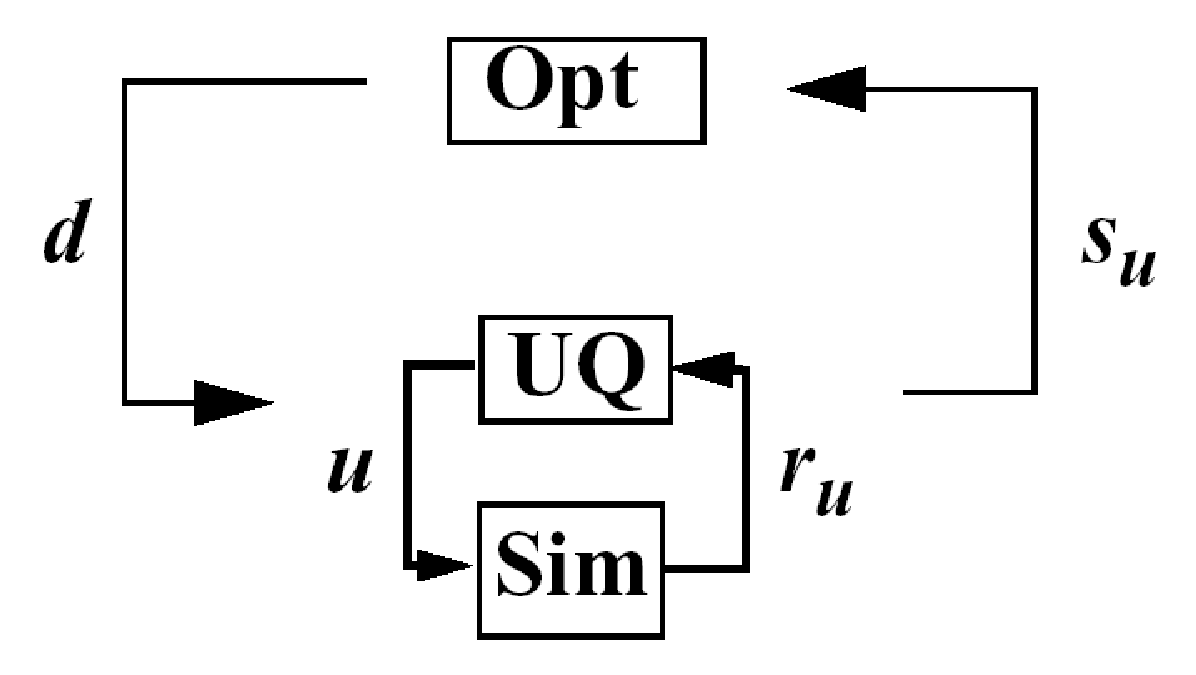
\includegraphics[scale=0.33]{images/nested_ouu}
  \caption{Formulation 1: Nested OUU.}
  \label{models:ex:figure08}
\end{figure}

Figure~\ref{models:ex:figure09} shows a DAKOTA input file for a nested
OUU example problem that is based on the textbook test problem. This
input file is named \texttt{dakota\_ouu1\_tb.in} in the
\texttt{Dakota/test} directory.  In this example, the objective
function contains two probability of failure estimates, and an
inequality constraint contains another probability of failure
estimate. For this example, failure is defined to occur when one of
the textbook response functions exceeds its threshold value. The
strategy keyword block at the top of the input file identifies this as
an OUU problem. The strategy keyword block is followed by the
optimization specification, consisting of the optimization method, the
continuous design variables, and the response quantities that will be
used by the optimizer. The mapping matrices used for incorporating UQ
statistics into the optimization response data are described in the
DAKOTA Reference Manual~\cite{RefMan}. The uncertainty quantification
specification includes the UQ method, the uncertain variable
probability distributions, the interface to the simulation code, and
the UQ response attributes. As with other complex DAKOTA input files,
the identification tags given in each keyword block can be used to
follow the relationships among the different keyword blocks.

\begin{figure}
  \centering
  \begin{bigbox}
    \begin{tiny}
      \verbatimtabinput[8]{dakota_ouu1_tb.in}
    \end{tiny}
  \end{bigbox}
  \caption{DAKOTA input file for the nested OUU example.}
  \label{models:ex:figure09}
\end{figure}

Latin hypercube sampling is used as the UQ method in this example
problem. Thus, each evaluation of the response functions by the
optimizer entails 50 Latin hypercube samples. In general, nested OUU
studies can easily generate several thousand function evaluations and
gradient-based optimizers may not perform well due to noisy or
insensitive statistics resulting from under-resolved sampling. These
observations motivate the use of surrogate-based approaches to OUU.

Other nested OUU examples in the \texttt{Dakota/test} directory
include \texttt{dakota\_ouu1\_tbch.in}, which adds an additional
interface for including deterministic data in the textbook OUU
problem, and\\ \texttt{dakota\_ouu1\_cantilever.in}, which solves the
cantilever OUU problem (see Section~\ref{additional:cantilever}) with
a nested approach. For each of these files, the ``\texttt{1}''
identifies formulation 1, which is short-hand for the nested approach.

% TO DO: combine with TR-SBOUU discussion?
\subsubsection{Surrogate-Based OUU (SBOUU)}\label{models:ex:ouu:sb}

Surrogate-based optimization under uncertainty strategies can be
effective in reducing the expense of OUU studies. Possible
formulations include use of a surrogate model at the optimization
level, at the uncertainty quantification level, or at both levels.
These surrogate models encompass both data fit surrogates (at the
optimization or UQ level) and model hierarchy surrogates (at the UQ
level only). Figure~\ref{models:ex:figure10} depicts the different
surrogate-based formulations where $\mathbf{\hat{r}_{u}}$ and
$\mathbf{\hat{s}_{u}}$ are approximate response functions and
approximate response statistics, respectively, generated from the
surrogate models.

\begin{figure}
  \centering
  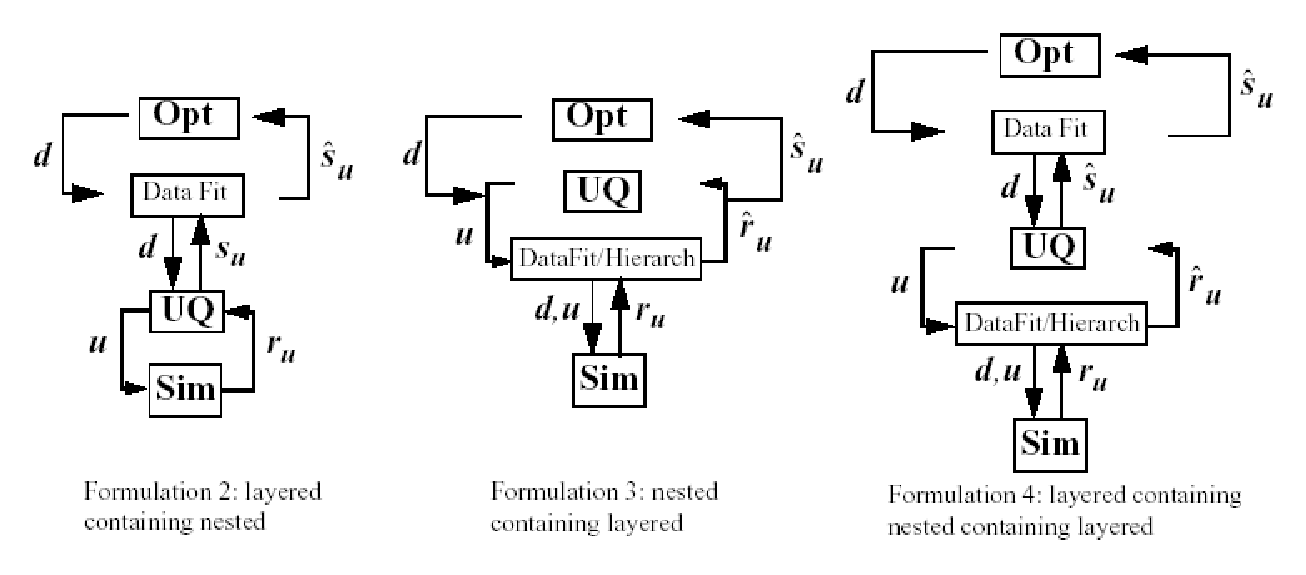
\includegraphics[scale=0.65]{images/sbouu}
  \caption{Formulations 2, 3, and 4 for Surrogate-based OUU.}
  \label{models:ex:figure10}
\end{figure}

SBOUU examples in the \texttt{Dakota/test} directory include
\texttt{dakota\_sbouu2\_tbch.in},\\ \texttt{dakota\_sbouu3\_tbch.in},
and \texttt{dakota\_sbouu4\_tbch.in}, which solve the textbook OUU
problem, and \texttt{dakota\_sbouu2\_cantilever.in},
\texttt{dakota\_sbouu3\_cantilever.in}, and\\
\texttt{dakota\_sbouu4\_cantilever.in}, which solve the cantilever OUU
problem (see Section~\ref{additional:cantilever}). For each of these
files, the ``\texttt{2},'' ``\texttt{3},'' and ``\texttt{4}'' identify
formulations 2, 3, and 4, which are short-hand for the ``layered
containing nested,'' ``nested containing layered,'' and ``layered
containing nested containing layered'' surrogate-based formulations,
respectively. In general, the use of surrogates greatly reduces the
computational expense of these OUU study. However, without restricting
and verifying the steps in the approximate optimization cycles,
weaknesses in the data fits can be exploited and poor solutions may be
obtained. The need to maintain accuracy of results leads to the use of
trust-region surrogate-based approaches.

\subsubsection{Trust-Region Surrogate-Based OUU (TR-SBOUU)}\label{models:ex:ouu:trsb}

The TR-SBOUU approach applies the trust region logic of deterministic
SBO (see Section~\ref{sbm:sblm}) to SBOUU. Trust-region verifications
are applicable when surrogates are used at the optimization level,
i.e., formulations 2 and 4. As a result of periodic verifications and
surrogate rebuilds, these techniques are more expensive than SBOUU;
however they are more reliable in that they maintain the accuracy of
results. Relative to nested OUU (formulation 1), TR-SBOUU tends to be
less expensive and less sensitive to initial seed and starting point.

TR-SBOUU examples in the \texttt{Dakota/test} directory include
\texttt{dakota\_trsbouu2\_tbch.in} and\\
\texttt{dakota\_trsbouu4\_tbch.in}, which solve the textbook OUU
problem, and\\ \texttt{dakota\_trsbouu2\_cantilever.in} and
\texttt{dakota\_trsbouu4\_cantilever.in}, which solve the cantilever
OUU problem (see Section~\ref{additional:cantilever}).

Computational results for several example problems are available
in~\cite{Eld02}.

\subsubsection{Bi-level RBDO} \label{models:ex:ouu:bilev_rbdo}

The simplest and most direct RBDO approach is the bi-level approach in
which a full reliability analysis is performed for every optimization
function evaluation.  This involves a nesting of two distinct levels
of optimization within each other, one at the design level and one at
the MPP search level.

Since an RBDO problem will typically specify both the $\bar{z}$ level
and the $\bar{p}/\bar{\beta}$ level, one can use either the RIA or the
PMA formulation for the UQ portion and then constrain the result in
the design optimization portion.  In particular, RIA reliability
analysis maps $\bar{z}$ to $p/\beta$, so RIA RBDO constrains $p/\beta$:
\begin{eqnarray}
  {\rm minimize }     & f \nonumber \\
  {\rm subject \ to } & \beta \ge \bar{\beta} \nonumber \\
  {\rm or }           & p \le \bar{p} \label{eq:rbdo_ria}
\end{eqnarray}

\noindent And PMA reliability analysis maps $\bar{p}/\bar{\beta}$ to 
$z$, so PMA RBDO constrains $z$:
\begin{eqnarray}
  {\rm minimize }     & f \nonumber \\
  {\rm subject \ to } & z \ge \bar{z} \label{eq:rbdo_pma}
\end{eqnarray}

\noindent where $z \ge \bar{z}$ is used as the RBDO constraint for 
a cumulative failure probability (failure defined as $z \le \bar{z}$)
but $z \le \bar{z}$ would be used as the RBDO constraint for a
complementary cumulative failure probability (failure defined as $z
\ge \bar{z}$).  It is worth noting that DAKOTA is not limited to these
types of inequality-constrained RBDO formulations; rather, they are
convenient examples.  DAKOTA supports general optimization under
uncertainty mappings~\cite{Eld02} which allow flexible use of
statistics within multiple objectives, inequality constraints, and
equality constraints.

In \texttt{Dakota/test}, the \texttt{dakota\_rbdo\_cantilever.in},
\texttt{dakota\_rbdo\_short\_column.in}, and\\
\texttt{dakota\_rbdo\_steel\_column.in} input files solve 
the cantilever (see Section~\ref{additional:cantilever}), short column
(see Section~\ref{additional:short_column}), and steel column (see
Section~\ref{additional:steel_column}) OUU problems using a bi-level
RBDO approach employing numerical design gradients.

An important performance enhancement for bi-level methods is the use
of sensitivity analysis to analytically compute the design gradients
of probability, reliability, and response levels.  When design
variables are separate from the uncertain variables (i.e., they are
not distribution parameters), then the following first-order 
expressions may be used~\cite{Hoh86,Kar92,All04}:
\begin{eqnarray}
\nabla_{\bf d} z           & = & \nabla_{\bf d} g \label{eq:deriv_z} \\
\nabla_{\bf d} \beta_{cdf} & = & \frac{1}{{\parallel \nabla_{\bf u} G 
\parallel}} \nabla_{\bf d} g \label{eq:deriv_beta} \\
\nabla_{\bf d} p_{cdf}     & = & -\phi(-\beta_{cdf}) \nabla_{\bf d} \beta_{cdf}
\label{eq:deriv_p}
\end{eqnarray}
where it is evident from Eqs.~\ref{eq:beta_cdf_ccdf}-\ref{eq:p_cdf_ccdf} 
that $\nabla_{\bf d} \beta_{ccdf} = -\nabla_{\bf d} \beta_{cdf}$ and 
$\nabla_{\bf d} p_{ccdf} = -\nabla_{\bf d} p_{cdf}$.  In the case of 
second-order integrations, Eq.~\ref{eq:deriv_p} must be expanded to 
include the curvature correction.  For Breitung's correction 
(Eq.~\ref{eq:p_2nd_breit}),
\begin{equation}
\nabla_{\bf d} p_{cdf} = \left[ \Phi(-\beta_p) \sum_{i=1}^{n-1} 
\left( \frac{-\kappa_i}{2 (1 + \beta_p \kappa_i)^{\frac{3}{2}}}
\prod_{\stackrel{\scriptstyle j=1}{j \ne i}}^{n-1} 
\frac{1}{\sqrt{1 + \beta_p \kappa_j}} \right) - 
\phi(-\beta_p) \prod_{i=1}^{n-1} \frac{1}{\sqrt{1 + \beta_p \kappa_i}} 
\right] \nabla_{\bf d} \beta_{cdf} \label{eq:deriv_p_breit}
\end{equation}
where $\nabla_{\bf d} \kappa_i$ has been neglected and $\beta_p \ge 0$
(see Section~\ref{uq:reliability:mpp:int}).  Other approaches assume
the curvature correction is nearly independent of the design
variables~\cite{Rac02}, which is equivalent to neglecting the first
term in Eq.~\ref{eq:deriv_p_breit}.

To capture second-order probability estimates within an RIA RBDO
formulation using well-behaved $\beta$ constraints, a generalized 
reliability index can be introduced where, similar to Eq.~\ref{eq:beta_cdf},
\begin{equation}
\beta^*_{cdf} = -\Phi^{-1}(p_{cdf}) \label{eq:gen_beta}
\end{equation}
for second-order $p_{cdf}$.  This reliability index is no longer
equivalent to the magnitude of ${\bf u}$, but rather is a convenience
metric for capturing the effect of more accurate probability
estimates.  The corresponding generalized reliability index
sensitivity, similar to Eq.~\ref{eq:deriv_p}, is
\begin{equation}
\nabla_{\bf d} \beta^*_{cdf} = -\frac{1}{\phi(-\beta^*_{cdf})}
\nabla_{\bf d} p_{cdf} \label{eq:deriv_gen_beta}
\end{equation}
where $\nabla_{\bf d} p_{cdf}$ is defined from Eq.~\ref{eq:deriv_p_breit}.
Even when $\nabla_{\bf d} g$ is estimated numerically,
Eqs.~\ref{eq:deriv_z}-\ref{eq:deriv_gen_beta} can be used to avoid
numerical differencing across full reliability analyses.

When the design variables are distribution parameters of the uncertain
variables, $\nabla_{\bf d} g$ is expanded with the chain rule and
Eqs.~\ref{eq:deriv_z} and~\ref{eq:deriv_beta} become
\begin{eqnarray}
\nabla_{\bf d} z           & = & \nabla_{\bf d} {\bf x} \nabla_{\bf x} g
\label{eq:deriv_z_ds} \\
\nabla_{\bf d} \beta_{cdf} & = & \frac{1}{{\parallel \nabla_{\bf u} G 
\parallel}} \nabla_{\bf d} {\bf x} \nabla_{\bf x} g \label{eq:deriv_beta_ds}
\end{eqnarray}
where the design Jacobian of the transformation ($\nabla_{\bf d} {\bf x}$)
may be obtained analytically for uncorrelated ${\bf x}$ or 
semi-analytically for correlated ${\bf x}$ ($\nabla_{\bf d} {\bf L}$
is evaluated numerically) by differentiating Eqs.~\ref{eq:trans_zx} 
and~\ref{eq:trans_zu} with respect to the distribution parameters.
Eqs.~\ref{eq:deriv_p}-\ref{eq:deriv_gen_beta} remain the same as
before.  For this design variable case, all required information for 
the sensitivities is available from the MPP search.

Since Eqs.~\ref{eq:deriv_z}-\ref{eq:deriv_beta_ds} are derived using
the Karush-Kuhn-Tucker optimality conditions for a converged MPP, they
are appropriate for RBDO using AMV+, AMV$^2$+, TANA, FORM, and SORM,
but not for RBDO using MVFOSM, MVSOSM, AMV, or AMV$^2$.

In \texttt{Dakota/test}, the
\texttt{dakota\_rbdo\_cantilever\_analytic.in} and\\
\texttt{dakota\_rbdo\_short\_column\_analytic.in} input files solve 
the cantilever and short column OUU problems using a bi-level RBDO
approach with analytic design gradients and first-order limit state
approximations.  The \texttt{dakota\_rbdo\_cantilever\_analytic2.in},
\texttt{dakota\_rbdo\_short\_column\_analytic2.in}, and 
\texttt{dakota\_rbdo\_steel\_column\_analytic2.in} input files 
also employ analytic design gradients, but are extended to employ
second-order limit state approximations and integrations.

\subsubsection{Sequential/Surrogate-based RBDO} \label{models:ex:ouu:surr_rbdo}

An alternative RBDO approach is the sequential approach, in which
additional efficiency is sought through breaking the nested
relationship of the MPP and design searches.  The general concept is
to iterate between optimization and uncertainty quantification,
updating the optimization goals based on the most recent probabilistic
assessment results.  This update may be based on safety
factors~\cite{Wu01} or other approximations~\cite{Du04}.

A particularly effective approach for updating the optimization goals
is to use the $p/\beta/z$ sensitivity analysis of
Eqs.~\ref{eq:deriv_z}-\ref{eq:deriv_beta_ds} in combination with local
surrogate models~\cite{Zou04}.  In \cite{Eld05} and~\cite{Eld06a},
first-order and second-order Taylor series approximations were
employed within a trust-region model management framework~\cite{Giu00}
in order to adaptively manage the extent of the approximations and
ensure convergence of the RBDO process.  Surrogate models were used
for both the objective function and the constraints, although the use
of constraint surrogates alone is sufficient to remove the nesting.

In particular, RIA trust-region surrogate-based RBDO employs surrogate
models of $f$ and $p/\beta$ within a trust region $\Delta^k$ centered
at ${\bf d}_c$.  For first-order surrogates:
\begin{eqnarray}
  {\rm minimize }     & f({\bf d}_c) + \nabla_d f({\bf d}_c)^T
({\bf d} - {\bf d}_c) \nonumber \\
  {\rm subject \ to } & \beta({\bf d}_c) + \nabla_d \beta({\bf d}_c)^T
({\bf d} - {\bf d}_c) \ge \bar{\beta} \nonumber \\
  {\rm or }           & p ({\bf d}_c) + \nabla_d p({\bf d}_c)^T 
({\bf d} - {\bf d}_c) \le \bar{p} \nonumber \\
& {\parallel {\bf d} - {\bf d}_c \parallel}_\infty \le \Delta^k
\label{eq:rbdo_surr1_ria}
\end{eqnarray}
and for second-order surrogates:
\begin{eqnarray}
  {\rm minimize }     & f({\bf d}_c) + \nabla_{\bf d} f({\bf d}_c)^T
({\bf d} - {\bf d}_c)  + \frac{1}{2} ({\bf d} - {\bf d}_c)^T 
\nabla^2_{\bf d} f({\bf d}_c) ({\bf d} - {\bf d}_c) \nonumber \\
  {\rm subject \ to } & \beta({\bf d}_c) + \nabla_{\bf d} \beta({\bf d}_c)^T
({\bf d} - {\bf d}_c) + \frac{1}{2} ({\bf d} - {\bf d}_c)^T 
\nabla^2_{\bf d} \beta({\bf d}_c) ({\bf d} - {\bf d}_c) \ge \bar{\beta}
\nonumber \\
  {\rm or }           & p ({\bf d}_c) + \nabla_{\bf d} p({\bf d}_c)^T 
({\bf d} - {\bf d}_c) + \frac{1}{2} ({\bf d} - {\bf d}_c)^T 
\nabla^2_{\bf d} p({\bf d}_c) ({\bf d} - {\bf d}_c) \le \bar{p} \nonumber \\
& {\parallel {\bf d} - {\bf d}_c \parallel}_\infty \le \Delta^k
\label{eq:rbdo_surr2_ria}
\end{eqnarray}
For PMA trust-region surrogate-based RBDO, surrogate models of
$f$ and $z$ are employed within a trust region $\Delta^k$ centered 
at ${\bf d}_c$.  For first-order surrogates:
\begin{eqnarray}
  {\rm minimize }     & f({\bf d}_c) + \nabla_d f({\bf d}_c)^T
({\bf d} - {\bf d}_c) \nonumber \\
  {\rm subject \ to } & z({\bf d}_c) + \nabla_d z({\bf d}_c)^T ({\bf d} - {\bf d}_c) 
\ge \bar{z} \nonumber \\
& {\parallel {\bf d} - {\bf d}_c \parallel}_\infty \le \Delta^k
\label{eq:rbdo_surr1_pma}
\end{eqnarray}
and for second-order surrogates:
\begin{eqnarray}
  {\rm minimize }     & f({\bf d}_c) + \nabla_{\bf d} f({\bf d}_c)^T
({\bf d} - {\bf d}_c) + \frac{1}{2} ({\bf d} - {\bf d}_c)^T 
\nabla^2_{\bf d} f({\bf d}_c) ({\bf d} - {\bf d}_c) \nonumber \\
  {\rm subject \ to } & z({\bf d}_c) + \nabla_{\bf d} z({\bf d}_c)^T ({\bf d} - {\bf d}_c)
 + \frac{1}{2} ({\bf d} - {\bf d}_c)^T \nabla^2_{\bf d} z({\bf d}_c) 
({\bf d} - {\bf d}_c) \ge \bar{z} \nonumber \\
& {\parallel {\bf d} - {\bf d}_c \parallel}_\infty \le \Delta^k
\label{eq:rbdo_surr2_pma}
\end{eqnarray}
where the sense of the $z$ constraint may vary as described
previously.  The second-order information in
Eqs.~\ref{eq:rbdo_surr2_ria} and \ref{eq:rbdo_surr2_pma} will
typically be approximated with quasi-Newton updates.

In \texttt{Dakota/test}, the
\texttt{dakota\_rbdo\_cantilever\_trsb.in} and\\
\texttt{dakota\_rbdo\_short\_column\_trsb.in} input files solve 
the cantilever and short column OUU problems using a first-order
sequential RBDO approach with analytic design gradients and
first-order limit state approximations.  The
\texttt{dakota\_rbdo\_cantilever\_trsb2.in},
\texttt{dakota\_rbdo\_short\_column\_trsb2.in}, and 
\texttt{dakota\_rbdo\_steel\_column\_trsb2.in} input files 
utilize second-order sequential RBDO approaches that employ
second-order limit state approximations and integrations (from
analytic limit state Hessians with respect to the uncertain variables)
and quasi-Newton approximations to the reliability metric Hessians
with respect to design variables.

\subsubsection{Stochastic Expansion-Based Design Optimization} \label{models:ex:ouu:sebdo}

Section~\ref{uq:expansion:rvsa} describes sensitivity analysis of the
polynomial chaos expansion with respect to the random variables.  Here
we extend this analysis to include sensitivity analysis with respect
to design variables.  With the introduction of design variables
$\boldsymbol{s}$, a polynomial chaos expansion only over the random
variables $\boldsymbol{\xi}$ has the functional relationship:
\begin{equation}
R(\boldsymbol{\xi}, \boldsymbol{s}) \cong \sum_{j=0}^P \alpha_j(\boldsymbol{s}) 
\Psi_j(\boldsymbol{\xi}) \label{eq:R_alpha_s_psi_xi}
\end{equation}

\noindent In this case, design sensitivities for the mean and variance 
in Eqs.~\ref{eq:mean_pce} and~\ref{eq:var_pce} are as follows:
\begin{eqnarray}
\frac{d\mu_R}{ds} &=& \frac{d\alpha_0}{ds} 
~~=~~ \frac{d}{ds} \langle R \rangle 
~~=~~ \langle \frac{dR}{ds} \rangle \label{eq:dmuR_ds_unc_pce} \\
\frac{d\sigma^2_R}{ds} &=& \sum_{j=1}^P \langle \Psi_j^2 \rangle 
\frac{d\alpha_j^2}{ds}
~~=~~ 2 \sum_{j=1}^P \alpha_j \langle \frac{dR}{ds}, \Psi_j \rangle 
\label{eq:dsigR_ds_unc_pce}
%2 \sigma_R \frac{d\sigma_R}{ds} &=& 2 
%\sum_{j=1}^P \alpha_j \frac{d\alpha_j}{ds} \langle \Psi_j^2 \rangle \\
%\frac{d\sigma_R}{ds} &=& \frac{1}{\sigma_R} 
%\sum_{j=1}^P \alpha_j \frac{d}{ds} \langle R, \Psi_j \rangle 
%\label{eq:dsigR_ds_unc_pce}
\end{eqnarray}
since
\begin{equation}
\frac{d\alpha_j}{ds} = \frac{\langle \frac{dR}{ds}, \Psi_j \rangle}
{\langle \Psi^2_j \rangle} \label{eq:dalpha_j_ds}
\end{equation}
The coefficients calculated in Eq.~\ref{eq:dalpha_j_ds} may be
interpreted as either the design sensitivities of the chaos
coefficients for the response expansion or the chaos coefficients of
an expansion for the response design sensitivities.  The evaluation of
integrals involving $\frac{dR}{ds}$ extends the data requirements for
the PCE approach to include response sensitivities at each of the
sampling points for the quadrature, sparse grid, sampling, or point
collocation coefficient estimation approaches.  The resulting
expansions are valid only for a particular set of design variables and
must be recalculated each time the design variables are modified.

Similarly for stochastic collocation,
\begin{equation}
R(\boldsymbol{\xi}, \boldsymbol{s}) \cong \sum_{j=1}^{N_p} r_j(\boldsymbol{s}) 
\boldsymbol{L}_j(\boldsymbol{\xi}) \label{eq:R_r_s_L_xi}
\end{equation}
leads to
\begin{eqnarray}
\frac{d\mu_R}{ds} &=& \frac{d}{ds} \langle R \rangle 
~~=~~ \sum_{j=1}^{N_p} \frac{dr_j}{ds} \langle \boldsymbol{L}_j \rangle 
~~=~~ \sum_{j=1}^{N_p} w_j \frac{dr_j}{ds} \label{eq:dmuR_ds_xi_sc} \\
\frac{d\sigma^2_R}{ds} &=& \sum_{j=1}^{N_p} 2 w_j r_j \frac{dr_j}{ds}
- 2 \mu_R \frac{d\mu_R}{ds} 
~~=~~ \sum_{j=1}^{N_p} 2 w_j (r_j - \mu_R) \frac{dr_j}{ds}
\label{eq:dsigR_ds_xi_sc}
\end{eqnarray}
based on differentiation of Eqs.~\ref{eq:mean_sc}-\ref{eq:var_sc}.

Alternatively, a stochastic expansion can be formed over both
$\boldsymbol{\xi}$ and $\boldsymbol{s}$.  Assuming a bounded
design domain $\boldsymbol{s}_L \le \boldsymbol{s} \le
\boldsymbol{s}_U$ (with no implied probability content), a Legendre 
chaos basis would be appropriate for each of the dimensions in 
$\boldsymbol{s}$ within a polynomial chaos expansion.
\begin{equation}
R(\boldsymbol{\xi}, \boldsymbol{s}) \cong \sum_{j=0}^P \alpha_j 
\Psi_j(\boldsymbol{\xi}, \boldsymbol{s}) \label{eq:R_alpha_psi_xi_s}
\end{equation}

\noindent In this case, design sensitivities for the mean and variance 
do not require response sensitivity data, but this comes at the cost
of forming the PCE over additional dimensions.  For this combined
variable expansion, the mean and variance are evaluated by evaluating
the expectations over only the random variables, which eliminates the
polynomial dependence on $\boldsymbol{\xi}$, leaving behind the
desired polynomial dependence on $\boldsymbol{s}$:
\begin{eqnarray}
\mu_R(\boldsymbol{s}) &=& \sum_{j=0}^P \alpha_j \langle \Psi_j(\boldsymbol{\xi},
\boldsymbol{s}) \rangle_{\boldsymbol{\xi}} \label{eq:muR_comb_pce} \\
\sigma^2_R(\boldsymbol{s}) &=& \sum_{j=0}^P \sum_{k=0}^P \alpha_j \alpha_k 
\langle \Psi_j(\boldsymbol{\xi}, \boldsymbol{s}) \Psi_k(\boldsymbol{\xi},
\boldsymbol{s}) \rangle_{\boldsymbol{\xi}} ~-~ \mu^2_R(\boldsymbol{s})
\label{eq:sigR_comb_pce}
\end{eqnarray}
The remaining polynomials may then be differentiated with respect to
$\boldsymbol{s}$. % as in Eqs.~\ref{eq:dR_dxi_pce}-\ref{eq:deriv_prod_pce}.
In this approach, the combined PCE is valid for the full design
variable range ($\boldsymbol{s}_L \le \boldsymbol{s} \le \boldsymbol{s}_U$)
and does not need to be updated for each change in design variables,
although adaptive localization techniques (i.e., trust region model
management approaches) can be employed when improved local accuracy of
the sensitivities is required.
% Q: how is TR ratio formed if exact soln can't be evaluated?
% A: if objective is accuracy over a design range, then truth is PCE/SC
%    at a single design point!  -->>  Can use first-order corrections based
%    on the 2 different SSA approaches!  This is a multifidelity SBO using
%    HF = Uncertain expansion, LF = Combined expansion. Should get data reuse.

Similarly for stochastic collocation,
\begin{equation}
R(\boldsymbol{\xi}, \boldsymbol{s}) \cong \sum_{j=1}^{N_p} r_j 
\boldsymbol{L}_j(\boldsymbol{\xi}, \boldsymbol{s}) \label{eq:R_r_L_xi_s}
\end{equation}
leads to
\begin{eqnarray}
\mu_R(\boldsymbol{s}) &=& \sum_{j=1}^{N_p} r_j \langle 
\boldsymbol{L}_j(\boldsymbol{\xi}, \boldsymbol{s}) \rangle_{\boldsymbol{\xi}} 
\label{eq:muR_both_sc} \\
\sigma^2_R(\boldsymbol{s}) &=& \sum_{j=1}^{N_p} \sum_{k=1}^{N_p} r_j r_k 
\langle \boldsymbol{L}_j(\boldsymbol{\xi}, \boldsymbol{s}) 
\boldsymbol{L}_k(\boldsymbol{\xi}, \boldsymbol{s}) \rangle_{\boldsymbol{\xi}}
~-~ \mu^2_R(\boldsymbol{s}) \label{eq:sigR_both_sc}
\end{eqnarray}
where the remaining polynomials not eliminated by the expectation over
$\boldsymbol{\xi}$ are again differentiated with respect to $\boldsymbol{s}$.

Given the capability to compute analytic statistics of the response
along with design sensitivities of these statistics, DAKOTA supports
bi-level, sequential, and multifidelity approaches for optimization
under uncertainty (OUU). %for reliability-based design and robust design.
The latter two approaches apply surrogate modeling approaches (data 
fits and multifidelity modeling) to the uncertainty analysis and then 
apply trust region model management to the optimization process.

The simplest and most direct approach is to employ these analytic
statistics and their design derivatives directly within an
optimization loop.  This approach is known as bi-level OUU, since
there is an inner level uncertainty analysis nested within an outer
level optimization.

Consider the common reliability-based design example of a deterministic 
objective function with a reliability constraint:
\begin{eqnarray}
  {\rm minimize }     & f \nonumber \\
  {\rm subject \ to } & \beta \ge \bar{\beta} \label{eq:rbdo}
\end{eqnarray}
where $\beta$ is computed relative to a prescribed threshold response
value $\bar{z}$ and is constrained by a prescribed reliability level
$\bar{\beta}$.  Another common example is robust design in which the
constraint enforcing a reliability lower-bound has been replaced with
a constraint enforcing a variance upper-bound:
\begin{eqnarray}
  {\rm minimize }     & f \nonumber \\
  {\rm subject \ to } & \sigma^2 \le \bar{\sigma}^2 \label{eq:rdo}
\end{eqnarray}
%It is worth noting that DAKOTA is not limited to these
%types of inequality-constrained OUU formulations; rather, they are
%convenient examples.  DAKOTA supports general optimization under
%uncertainty mappings~\cite{sbouu} which allow flexible use of
%statistics within multiple objectives, inequality constraints, and
%equality constraints.

Solving these problems using a bi-level approach involves computing
$\beta(\boldsymbol{s})$ and $\frac{d\beta}{d\boldsymbol{s}}$ for
Eq.~\ref{eq:rbdo} or $\sigma^2$ and $\frac{d\sigma^2}{d\boldsymbol{s}}$
for Eq.~\ref{eq:rdo} for each set of design variables $\boldsymbol{s}$
passed from the optimizer.  This approach is supported for both 
Uncertain and Combined expansions using PCE and SC.

An alternative OUU approach is the sequential approach, in which
additional efficiency is sought through breaking the nested
relationship of the UQ and optimization loops.  The general concept is
to iterate between optimization and uncertainty quantification,
updating the optimization goals based on the most recent uncertainty
assessment results.  This approach is common with the reliability
methods community, for which the updating strategy may be based on
safety factors~\cite{Wu01} or other approximations~\cite{Du04}.

A particularly effective approach for updating the optimization goals
is to use data fit surrogate models, and in particular, local Taylor
series models allow direct insertion of stochastic sensitivity
analysis capabilities.  In Ref.~\cite{Eld05}, first-order Taylor
series approximations were explored, and in Ref.~\cite{Eld06a},
second-order Taylor series approximations are investigated.  In both
cases, a trust-region model management framework~\cite{Eld06b} is
used to adaptively manage the extent of the approximations and ensure
convergence of the OUU process.  Surrogate models are used for both
the objective and the constraint functions, although the use of
surrogates is only required for the functions containing statistical
results; deterministic functions may remain explicit is desired.

In particular, trust-region surrogate-based optimization for
reliability-based design employs surrogate models of $f$ and $\beta$
within a trust region $\Delta^k$ centered at ${\bf s}_c$:
\begin{eqnarray}
  {\rm minimize }     & f({\bf s}_c) + \nabla_s f({\bf s}_c)^T
({\bf s} - {\bf s}_c) \nonumber \\
  {\rm subject \ to } & \beta({\bf s}_c) + \nabla_s \beta({\bf s}_c)^T
({\bf s} - {\bf s}_c) \ge \bar{\beta} \\
& {\parallel {\bf s} - {\bf s}_c \parallel}_\infty \le \Delta^k \nonumber
\label{eq:rbdo_surr}
\end{eqnarray}
and trust-region surrogate-based optimization for robust design
employs surrogate models of $f$ and $\sigma^2$ within a trust region
$\Delta^k$ centered at ${\bf s}_c$:
\begin{eqnarray}
  {\rm minimize }     & f({\bf s}_c) + \nabla_s f({\bf s}_c)^T
({\bf s} - {\bf s}_c) \nonumber \\
  {\rm subject \ to } & \sigma^2({\bf s}_c) + \nabla_s \sigma^2({\bf s}_c)^T 
({\bf s} - {\bf s}_c) \le \bar{\sigma}^2 \\
& {\parallel {\bf s} - {\bf s}_c \parallel}_\infty \le \Delta^k \nonumber
\label{eq:rdo_surr}
\end{eqnarray}
Second-order local surrogates may also be employed, where the Hessians
are typically approximated with quasi-Newton updates.  The sequential
approach is available for Uncertain expansions using PCE and SC.

The multifidelity OUU approach is another trust-region surrogate-based
approach.  Instead of the surrogate UQ model being a simple data fit
(in particular, first-/second-order Taylor series model) of the truth
UQ model results, we now employ distinct UQ models of differing
fidelity.  This differing UQ fidelity could stem from the fidelity of
the underlying simulation model, the fidelity of the UQ algorithm, or
both.  In this paper, we focus on the fidelity of the UQ algorithm.
For reliability methods, this could entail varying fidelity in
approximating assumptions (e.g., Mean Value for low fidelity, SORM for
high fidelity), and for stochastic expansion methods, it could involve
differences in selected levels of $p$ and $k$ refinement.

%Here we will explore multifidelity stochastic models and employ
%first-order additive corrections, where the meaning of multiple
%fidelities is expanded to imply the quality of multiple UQ analyses,
%not necessarily the fidelity of the underlying simulation model.  For
%example, taking an example from the reliability method family, one
%might employ the simple Mean Value method as a ``low fidelity'' UQ
%model and take SORM as a ``high fidelity'' UQ model.  In this case,
%the models do not differ in their ability to span a range of design
%parameters; rather, they differ in their sets of approximating
%assumptions about the characteristics of the response function.

Here, we define UQ fidelity as point-wise accuracy in the
design space and take the low fidelity model, whose validity over the
design space will be adaptively controlled, to be the Combined
expansion PCE/SC model, and the high fidelity truth model to be the
Uncertain expansion PCE/SC model, with validity only at a single
design point.  This will allow us to take advantage of the design
space spanning and lower cost of the Combined expansion approach to
the extent possible, with fallback to the greater accuracy and higher
expense of the Uncertain expansion approach when needed.  The Combined
expansion approach will span only the current trust region of the
design space and will need to be reconstructed for each new trust region.  
%While conceptually different, in the end, this approach is
%similar to the use of a global data fit surrogate-based optimization
%at the top level in combination with the Uncertain expansion PCE/SC at
%the lower level, with the distinction that the multifidelity approach
%embeds the design space spanning within a modified PCE/SC process
%whereas the data fit approach performs the design space spanning
%outside of the UQ (using data from a single unmodified PCE/SC process,
%which may now remain zeroth-order).
The design derivatives of each model provide the necessary data
to correct the low fidelity model to first-order consistency with the
high fidelity model at the center of each trust region.

Multifidelity optimization for reliability-based design can be
formulated as:
\begin{eqnarray}
  {\rm minimize }     & f({\bf s}) \nonumber \\
  {\rm subject \ to } & \hat{\beta_{hi}}({\bf s}) \ge \bar{\beta} \\
& {\parallel {\bf s} - {\bf s}_c \parallel}_\infty \le \Delta^k \nonumber
\label{eq:rbdo_mf}
\end{eqnarray}
and multifidelity optimization for robust design can be formulated as:
\begin{eqnarray}
  {\rm minimize }     & f({\bf s}) \nonumber \\
  {\rm subject \ to } & \hat{\sigma_{hi}}^2({\bf s}) \le \bar{\sigma}^2 \\
& {\parallel {\bf s} - {\bf s}_c \parallel}_\infty \le \Delta^k \nonumber
\label{eq:rdo_mf}
\end{eqnarray}
where the deterministic objective function is not approximated and 
$\hat{\beta_{hi}}$ and $\hat{\sigma_{hi}}^2$ are the approximated
high-fidelity UQ results resulting from correction of the low-fidelity 
UQ results.  In the case of an additive correction function:
\begin{eqnarray}
\hat{\beta_{hi}}({\bf s})    &=& \beta_{lo}({\bf s}) + 
\alpha_{\beta}({\bf s})  \label{eq:corr_lf_beta} \\
\hat{\sigma_{hi}}^2({\bf s}) &=& \sigma_{lo}^2({\bf s}) + 
\alpha_{\sigma^2}({\bf s}) \label{eq:corr_lf_sigma}
\end{eqnarray}
where correction functions $\alpha({\bf s})$ enforcing first-order
%and quasi-second-order 
consistency~\cite{Eld04} are typically employed.

In \texttt{Dakota/test}, the \texttt{dakota\_pcbdo\_cantilever.in},
\texttt{dakota\_pcbdo\_rosenbrock.in},\\
\texttt{dakota\_pcbdo\_short\_column.in}, and
\texttt{dakota\_pcbdo\_steel\_column.in} input files solve 
cantilever (see Section~\ref{additional:cantilever}), Rosenbrock,
short column (see Section~\ref{additional:short_column}), and steel
column (see Section~\ref{additional:steel_column}) OUU problems using
a bi-level polynomial chaos-based approach, where the statistical
design metrics are reliability indices based on moment projection
(i.e., Eqs.~\ref{eq:mv_ria_cdf}-\ref{eq:mv_ria_ccdf}).  The test
matrix in the former three input files evaluate design gradients of
these reliability indices using several different approaches: analytic
design gradients based on a PCE formed over only over the random
variables (Eqs.~\ref{eq:dmuR_ds_unc_pce}-\ref{eq:dsigR_ds_unc_pce}),
analytic design gradients based on a PCE formed over all variables
(differentiation of
Eqs.~\ref{eq:muR_comb_pce}-\ref{eq:sigR_comb_pce}), numerical design
gradients based on a PCE formed only over the random variables, and
numerical design gradients based on a PCE formed over all variables.
In the cases where the expansion is formed over all variables, only a
single PCE construction is required for the complete PCBDO process,
whereas the expansions only over the random variables must be
recomputed for each change in design variables.  Sensitivities for
``augmented'' design variables (which are separate from and augment
the random variables) may be handled using either analytic approach;
however, sensitivities for ``inserted'' design variables (which define
distribution parameters for the random variables) must be handled
using Eqs.~\ref{eq:dmuR_ds_unc_pce}-\ref{eq:dsigR_ds_unc_pce} where
$\frac{dR}{ds}$ is calculated as $\frac{dR}{dx} \frac{dx}{ds}$.
Additional test input files include:
\begin{itemize}
\item \texttt{dakota\_scbdo\_cantilever.in}, 
\texttt{dakota\_scbdo\_rosenbrock.in}, \\
\texttt{dakota\_scbdo\_short\_column.in}, and
\texttt{dakota\_scbdo\_steel\_column.in} input files solve 
cantilever, Rosenbrock, short column, and steel column OUU problems
using a bi-level stochastic collocation-based approach.

\item \texttt{dakota\_pcbdo\_cantilever\_trsb.in},
\texttt{dakota\_pcbdo\_rosenbrock\_trsb.in}, \\
\texttt{dakota\_pcbdo\_short\_column\_trsb.in}, 
\texttt{dakota\_pcbdo\_steel\_column\_trsb.in},\\
\texttt{dakota\_scbdo\_cantilever\_trsb.in}, 
\texttt{dakota\_scbdo\_rosenbrock\_trsb.in}, \\
\texttt{dakota\_scbdo\_short\_column\_trsb.in}, and
\texttt{dakota\_scbdo\_steel\_column\_trsb.in} input files solve 
cantilever, Rosenbrock, short column, and steel column OUU problems
using sequential polynomial chaos-based and stochastic
collocation-based approaches.

\item \texttt{dakota\_pcbdo\_cantilever\_mf.in},
\texttt{dakota\_pcbdo\_rosenbrock\_mf.in}, \\
\texttt{dakota\_pcbdo\_short\_column\_mf.in}, 
\texttt{dakota\_scbdo\_cantilever\_mf.in}, \\
\texttt{dakota\_scbdo\_rosenbrock\_mf.in}, and
\texttt{dakota\_scbdo\_short\_column\_mf.in} input files solve 
cantilever, Rosenbrock, and short column OUU problems
using multifidelity polynomial chaos-based and stochastic
collocation-based approaches.
\end{itemize}


\subsubsection{Epistemic OUU} \label{models:ex:ouu:epistemic}

An emerging capability is optimization under epistemic uncertainty.
As described in the Nested Model section of the Reference
Manual~\cite{RefMan}, epistemic and mixed aleatory/epistemic
uncertainty quantification methods generate lower and upper interval
bounds for all requested response, probability, reliability, and
generalized reliability level mappings.  Design for robustness in the
presence of epistemic uncertainty could simply involve minimizing the
range of these intervals (subtracting lower from upper using the
nested model response mappings), and design for reliability in the
presence of epistemic uncertainty could involve controlling the worst
case upper or lower bound of the interval.

We now have the capability to perform epistemic analysis by 
using interval optimization on the ``outer loop'' to calculate bounding 
statistics of the aleatory uncertainty on the ``inner loop.''  
Preliminary studies~\cite{Eldred09} have shown this approach is more efficient 
and accurate than nested sampling (which was described in 
Section~\ref{models:ex:sop}.  This approach uses 
an efficient global optimization method for the outer loop and 
stochastic expansion methods (e.g. polynomial chaos or stochastic 
collocation on the inner loop).  The interval optimization is described in 
Section~\ref{uq:interval}.  Example input files demonstrating 
the use of interval estimation for epistemic analysis, 
specifically in epistemic-aleatory nesting, are: 
\texttt{dakota\_uq\_cantilever\_sop\_exp.in}, and
\texttt{dakota\_short\_column\_sop\_exp.in}. 

\subsection{Surrogate-Based Uncertainty Quantification} \label{models:ex:sbuq}

Many uncertainty quantification (UQ) methods are computationally costly. 
For example, sampling often requires many function evaluations to obtain 
accurate estimates of moments or percentile values of an output distribution.  
One approach to overcome the computational cost of sampling is to 
evaluate the true function (e.g. run the analysis driver) on a fixed, small
set of samples, use these sample evaluations to 
create a response surface approximation (e.g. a surrogate model or meta-model)
of the underlying ``true'' function, then perform random sampling (using 
thousands or millions of samples) on the approximation to obtain estimates 
of the mean, variance, and percentiles of the response. 

This approach, called ``surrogate-based uncertainty quantification'' 
is easy to do in DAKOTA, and one can set up input files to compare the 
results using no approximation (e.g. determine the mean, variance, and 
percentiles of the output directly based on the initial sample values) 
with the results obtained by sampling a variety of surrogate approximations.  
Example input files of a standard UQ analysis based on sampling alone vs. 
sampling a surrogate are shown in the \texttt{dakota\_uq\_sampling.in} and 
\texttt{dakota\_surr\_uq.in} in the \texttt{Dakota/examples/methods}
directory. 

Note that one must exercise some caution when using surrogate-based methods 
for uncertainty quantification. In general, there is not a single, 
straightforward approach to incorporate the error of the surrogate fit 
into the uncertainty estimates of the output produced by sampling the surrogate.
Two references which discuss some of the related 
issues are~\cite{Giu06} and~\cite{Swi06}. The first reference shows that 
statistics of a response based on a surrogate model were less accurate, and 
sometimes biased, for surrogates constructed on very small sample sizes.  
In many cases, however,~\cite{Giu06} shows that surrogate-based UQ performs 
well and sometimes generates more accurate estimates of statistical
quantities on the output.  The second reference goes into more detail 
about the interaction between sample type and response surface type (e.g., 
are some response surfaces more accurate when constructed on a particular 
sample type such as LHS vs. an orthogonal array?) In general, there is not 
a strong dependence of the surrogate performance with respect to sample type, 
but some sample types perform better with respect to some metrics and not 
others (for example, a Hammersley sample may do well at lowering root mean 
square error of the surrogate fit but perform poorly at lowering the maximum 
absolute deviation of the error).  Much of this work is empirical and 
application dependent.  If you choose to use surrogates in uncertainty 
quantification, we strongly recommend trying a variety of surrogates 
and examining diagnostic goodness-of-fit metrics. 

\chapter{Variables}\label{variables}

\section{Overview}\label{variables:overview}

The \texttt{variables} specification in a Dakota input file specifies
the parameter set to be iterated by a particular method. In the case
of an optimization study, these variables are adjusted in order to
locate an optimal design; in the case of parameter studies/sensitivity
analysis/design of experiments, these parameters are perturbed to
explore the parameter space; and in the case of uncertainty analysis,
the variables are associated with distribution/interval
characterizations which are used to compute corresponding
distribution/interval characterizations for response functions. To
accommodate these and other types of studies, Dakota supports design,
uncertain, and state variable types for continuous and discrete
variable domains.  Uncertain types can be further categorized as
either aleatory or epistemic, and discrete domains can include
discrete range, discrete integer set, discrete string set, and
discrete real set.

This chapter will present a brief overview of the main types of
variables and their uses, as well as cover some user issues relating
to file formats and the active set vector.  For a detailed description
of variables section syntax and example specifications, refer to the
variables keywords in the Dakota Reference Manual~\cite{RefMan}.


\section{Design Variables}\label{variables:design}

Design variables are those variables which are modified in the course
of determining an optimal design. These variables may be continuous
(real-valued between bounds), discrete range (integer-valued between
bounds), discrete set of integers (integer-valued from finite set),
discrete set of strings (string-valued from finite set), and discrete
set of reals (real-valued from finite set).

\subsection{Continuous Design Variables}\label{variables:design:cdv}

The most common type of design variables encountered in engineering
applications are of the continuous type. These variables may assume
any real value (e.g., \texttt{12.34}, \texttt{-1.735e+07}) within
their bounds. All but a handful of the optimization algorithms in
Dakota support continuous design variables exclusively.

\subsection{Discrete Design Variables}\label{variables:design:ddv}

Engineering design problems may contain discrete variables such as
material types, feature counts, stock gauge selections, etc. These
variables may assume only a fixed number of values, as compared to a
continuous variable which has an uncountable number of possible values
within its range.  Discrete variables may involve a range of
consecutive integers ($x$ can be any integer between \texttt{1} and
\texttt{10}), a set of integer values ($x$ can be \texttt{101},
\texttt{212}, or \texttt{355}), a set of string values ($x$ can be
\texttt{'direct'}, \texttt{'gmres'}, or \texttt{'jacobi'}), or a set
of real values (e.g., $x$ can be identically \texttt{4.2},
\texttt{6.4}, or \texttt{8.5}).

Discrete variables may be classified as either ``categorical'' or
``noncategorical.''  In the latter noncategorical case, the discrete
requirement can be relaxed during the solution process since the model
can still compute meaningful response functions for values outside the
allowed discrete range or set. For example, a discrete variable
representing the thickness of a structure is generally a
noncategorical variable since it can assume a continuous range of
values during the algorithm iterations, even if it is desired to have
a stock gauge thickness in the end. In the former categorical case,
the discrete requirement cannot be relaxed since the model cannot
obtain a solution for values outside the range or set. For example,
feature counts are generally categorical discrete variables, since
most computational models will not support a non-integer value for the
number of instances of some feature (e.g., number of support
brackets).  Dakota supports a \texttt{categorical} specification to
indicate which discrete real and discrete integer variables are
restricted vs. relaxable.  String variables cannot be relaxed.
  
Gradient-based optimization methods cannot be directly applied to
problems with discrete variables since derivatives only exist for a
variable continuum. For problems with noncategorical variables, the
experimental branch and bound capability (\texttt{branch\_and\_bound})
can be used to relax the discrete requirements and apply
gradient-based methods to a series of generated subproblems. For
problems with categorical variables, nongradient-based methods (e.g.,
\texttt{coliny\_ea}) are commonly used; however, most of those methods
do not take advantage of any structure that may be associated with the
categorical variables.  The exception is
\texttt{mesh\_adaptive\_search}.  If it is possible to define a
subjective relationship between the different values a given
categorical variable can take on, the user can communicate that
relationship in the form of an adjacency matrix.  The
\texttt{mesh\_adaptive\_search} will take that relationship into
consideration.  Further documentation can be found in~\cite{RefMan}
under the keywords \texttt{adjacency\_matrix} and
\texttt{neighbor\_order}.  Branch and bound techniques are discussed
in Section~\ref{adv_meth:minlp} and nongradient-based methods are
further described in Chapter~\ref{opt}.

In addition to engineering applications, many non-engineering
applications in the fields of scheduling, logistics, and resource
allocation contain discrete design parameters. Within the Department
of Energy, solution techniques for these problems impact programs in
stockpile evaluation and management, production planning,
nonproliferation, transportation (routing, packing, logistics),
infrastructure analysis and design, energy production, environmental
remediation, and tools for massively parallel computing such as domain
decomposition and meshing.

\subsubsection{Discrete Design Integer Variables}\label{variables:design:ddiv}

There are two types of discrete design integer variables supported by
Dakota.
\begin{itemize}

\item  The \texttt{discrete\_design\_range} specification supports a
range of consecutive integers between specified \texttt{lower\_bounds}
and \texttt{upper\_bounds}.

\item The \texttt{discrete\_design\_set integer} specification supports 
a set of enumerated integer values through the \texttt{elements} 
specification.  The set of values specified is stored internally as an 
STL set container, which enforces an ordered, unique representation of 
the integer data.  Underlying this set of ordered, unique integers is a 
set of indices that run from 0 to one less than the number of set values.
These indices are used by some iterative algorithms (e.g., parameter 
studies, SCOLIB iterators) for simplicity in discrete value enumeration 
when the actual corresponding set values are immaterial.  In the case of 
parameter studies, this index representation is exposed through certain 
step and partition control specifications (see Chapter~\ref{ps}).

\end{itemize}

\subsubsection{Discrete Design String Variables}\label{variables:design:ddsv}

There is one type of discrete design string variable supported by
Dakota.
\begin{itemize}

\item The \texttt{discrete\_design\_set string} specification
supports a set of enumerated string values through the
\texttt{elements} specification.  As for the discrete integer
set variables described in Section~\ref{variables:design:ddiv},
internal storage of the set values is ordered and unique and an
underlying index representation is exposed for the specification of
some iterative algorithms.

\end{itemize}
Each string element value must be quoted in the Dakota input file and
may contain alphanumeric, dash, underscore, and colon. White space,
quote characters, and backslash/meta-characters are not permitted.

\subsubsection{Discrete Design Real Variables}\label{variables:design:ddrv}

There is one type of discrete design real variable supported by
Dakota.
\begin{itemize}

\item The \texttt{discrete\_design\_set real} specification
specification supports a set of enumerated real values through the
\texttt{set\_values} specification.  As for the discrete integer
set variables described in Section~\ref{variables:design:ddiv},
internal storage of the set values is ordered and unique and an
underlying index representation is exposed for the specification of
some iterative algorithms.

\end{itemize}


\section{Uncertain Variables}\label{variables:uncertain}


Deterministic variables (i.e., those with a single known value) do not
capture the behavior of the input variables in all situations. In many
cases, the exact value of a model parameter is not precisely known. An
example of such an input variable is the thickness of a heat treatment
coating on a structural steel I-beam used in building construction.
Due to variability and tolerances in the coating process, the
thickness of the layer is known to follow a normal distribution with a
certain mean and standard deviation as determined from experimental
data. The inclusion of the uncertainty in the coating thickness is
essential to accurately represent the resulting uncertainty in the
response of the building.

\subsection{Aleatory Uncertain Variables}\label{variables:uncertain:auv}

Aleatory uncertainties are irreducible variabilities inherent in
nature.  They are characterized by having a sufficiently rich set of
data as to allow modeling using probability distributions, and
probabilistic methods are commonly used for propagating input aleatory
uncertainties described by probability distribution specifications.
The two following sections describe the continuous and discrete
aleatory uncertain variables supported by Dakota.

For aleatory random variables, Dakota supports a user-supplied
correlation matrix to provide correlations among the input
variables. By default, the correlation matrix is set to the identity
matrix, i.e., no correlation among the uncertain variables.

For additional information on random variable probability
distributions, refer to~\cite{Hal00} and~\cite{Swi04}. Refer to the Dakota
Reference Manual~\cite{RefMan} for more detail on the uncertain variable
specifications and to Chapter~\ref{uq} for a description of methods
available to quantify the uncertainty in the response.

\subsubsection{Continuous Aleatory Uncertain Variables}\label{variables:uncertain:cauv}

\begin{itemize}

\item Normal: a probability distribution characterized by a mean and 
  standard deviation. Also referred to as Gaussian. Bounded normal is
  also supported by some methods with an additional specification of
  lower and upper bounds.

\item Lognormal: a probability distribution characterized by a mean 
  and either a standard deviation or an error factor. The natural
  logarithm of a lognormal variable has a normal distribution. Bounded
  lognormal is also supported by some methods with an additional
  specification of lower and upper bounds.

\item Uniform: a probability distribution characterized by a lower bound 
  and an upper bound.  Probability is constant between the bounds.

\item Loguniform: a probability distribution characterized by a lower 
  bound and an upper bound.  The natural logarithm of a loguniform
  variable has a uniform distribution.

\item Triangular: a probability distribution characterized by a mode, a 
  lower bound, and an upper bound.

\item Exponential: a probability distribution characterized by a beta parameter.

\item Beta: a flexible probability distribution characterized by a lower 
  bound and an upper bound and alpha and beta parameters.  The uniform 
  distribution is a special case.

\item Gamma: a flexible probability distribution characterized by alpha 
  and beta parameters.  The exponential distribution is a special case.

\item Gumbel: the Type I Largest Extreme Value probability distribution.  
  Characterized by alpha and beta parameters.

\item Frechet: the Type II Largest Extreme Value probability distribution.  
  Characterized by alpha and beta parameters.

\item Weibull: the Type III Smallest Extreme Value probability distribution.  
  Characterized by alpha and beta parameters.

\item Histogram Bin: an empirically-based probability distribution 
  characterized by a set of $(x,y)$ pairs that map out
  histogram bins (a continuous interval with associated bin count).

\end{itemize}

\subsubsection{Discrete Aleatory Uncertain Variables}\label{variables:uncertain:dauv}

The following types of discrete aleatory uncertain variables are available:

\begin{itemize}

\item Poisson: integer-valued distribution used to predict the number of 
  discrete events that happen in a given time interval.

\item Binomial: integer-valued distribution used to predict 
  the number of failures in a number of independent tests or trials.

\item Negative Binomial: integer-valued distribution used to predict the
  number of times to perform a test to have a target number of successes.

\item Geometric: integer-valued distribution used to model the number of 
  successful trials that might occur before a failure is observed.

\item Hypergeometric: integer-valued distribution used to model the number 
  of failures observed in a set of tests that has a known proportion of 
  failures.

\item Histogram Point (integer, string, real): an empirically-based
  probability distribution characterized by a set of integer-valued
  $(i,c)$, string-valued $(s,c)$, and/or real-valued ${r,c}$ pairs
  that map out histogram points (each a discrete point value $i$, $s$,
  or $r$, with associated count $c$).

\end{itemize}


\subsection{Epistemic Uncertain Variables}\label{variables:uncertain:euv}

Epistemic uncertainties are reducible uncertainties resulting from a
lack of knowledge.  For epistemic uncertainties, data is generally
sparse, making the use of probability theory questionable and leading
to nonprobabilistic methods based on interval or fuzzy specifications.  Dakota
currently supports the following epistemic uncertain variable types.

\subsubsection{Continuous Epistemic Uncertain Variables}\label{variables:uncertain:ceuv}

\begin{itemize}

\item Continuous Interval: a real-valued interval-based specification
  characterized by sets of lower and upper bounds and Basic
  Probability Assignments (BPAs) associated with each interval.  The
  intervals may be overlapping, contiguous, or disjoint, and a single
  interval (with probability = 1) per variable is an important special
  case.  The interval distribution is not a probability distribution,
  as the exact structure of the probabilities within each interval is
  not known.  It is commonly used with epistemic uncertainty methods.

\end{itemize}


\subsubsection{Discrete Epistemic Uncertain Variables}\label{variables:uncertain:deuv}

\begin{itemize}

\item Discrete Interval: an integer-valued variant of the Continuous
  Interval described above (~\ref{variables:uncertain:ceuv}).

\item Discrete Set (integer, string, and real): Similar to discrete
  design set variables~\ref{variables:design:ddv}, these epistemic
  variables admit a finite number of values (elements) for type
  integer, string, or real, each with an associated probability.

\end{itemize}


\section{State Variables}\label{variables:state}

State variables consist of ``other'' variables which are to be mapped
through the simulation interface, in that they are not to be used for
design and they are not modeled as being uncertain. State variables
provide a convenient mechanism for parameterizing additional model
inputs which, in the case of a numerical simulator, might include
solver convergence tolerances, time step controls, or mesh fidelity
parameters. For additional model parameterizations involving strings
(e.g., ``mesh1.exo''), refer to the analysis components specification
described in Section~\ref{variables:parameters:standard} and in the
Interface Commands chapter of the Dakota Reference
Manual~\cite{RefMan}.  Similar to the design variables discussed in
Section~\ref{variables:design}, state variables can be specified with
a continuous range (real-valued between bounds), a discrete range
(integer-valued between bounds), a discrete integer-valued set, a
discrete string-valued set, or a discrete real-valued set.

State variables, as with other types of variables, are viewed
differently depending on the method in use. Since these variables are
neither design nor uncertain variables, algorithms for optimization,
least squares, and uncertainty quantification do not iterate on these
variables; i.e., they are not active and are hidden from the
algorithm. However, Dakota still maps these variables through the
user's interface where they affect the computational model in use.
This allows optimization, least squares, and uncertainty
quantification studies to be executed under different simulation
conditions (which will result, in general, in different results).
Parameter studies and design of experiments methods, on the other
hand, are general-purpose iterative techniques which do not draw a
distinction between variable types. They include state variables in
the set of variables to be iterated, which allows these studies to
explore the effect of state variable values on the response data of
interest.

In the future, state variables might be used in direct coordination
with an optimization, least squares, or uncertainty quantification
algorithm. For example, state variables could be used to enact model
adaptivity through the use of a coarse mesh or loose solver tolerances
in the initial stages of an optimization with continuous model
refinement as the algorithm nears the optimal solution.

\section{Management of Mixed Variables by Iterator}\label{variables:mixed}

\subsection{View}\label{variables:mixedview}
As alluded to in the previous section, the iterative method selected
for use in Dakota partially determines what subset, or view, 
of the variables data is active in the iteration. 
(Section~\ref{variables:precedence} contains a discussion of
how user overrides, response function type, and method are used to determine 
active variable view.) The general case of having 
a mixture of various different types of variables is supported 
within all of the Dakota methods even though certain methods will 
only modify certain types of variables (e.g., optimizers and least squares 
methods only modify design variables, and uncertainty quantification methods 
typically only utilize uncertain variables).  This implies that variables 
which are not under the direct control of a particular iterator will be 
mapped through the interface in an unmodified state. This allows for a 
variety of parameterizations within the model in addition to those which are
being used by a particular iterator, which can provide the convenience
of consolidating the control over various modeling parameters in a
single file (the Dakota input file). An important related point is
that the variable set that is active with a particular iterator is the
same variable set for which derivatives are typically computed (see
Section~\ref{responses:active}).

There are certain situations where the user may want to explicitly 
control the subset of variables that is considered active for a 
certain Dakota method.  This is done by specifying the keyword 
\texttt{active} in the variables specification block, followed by 
one of the following:  \texttt{all}, \texttt{design}, \texttt{uncertain},
\texttt{aleatory}, \texttt{epistemic}, or \texttt{state}.  
Specifying one of these subsets of variables will allow the 
Dakota method to operate on the specified variable types and override 
the defaults.  For example, the default behavior for a 
nondeterministic sampling method is to sample the uncertain 
variables.  However, if the user specified \texttt{active}  \texttt{all} 
in the variables specification block, the sampling would be performed 
over all variables (e.g. design and state variables as well as 
uncertain variables).  This may be desired in situations such as 
surrogate based optimization under uncertainty, where a surrogate may 
be built over both design and uncertain variables.  
Another situation where one may want the fine-grained control 
available by specifying one of these variable types is when one 
has state variables but only wants to sample over the design 
variables when constructing a surrogate model.  Finally, 
more sophisticated uncertainty studies may involve various 
combinations of epistemic vs. aleatory variables being active 
in nested models.

\subsection{Domain}\label{variables:domain}
Another control that the user can specify in the variables
specification block controls the domain type.  We have two domains
currently: mixed and relaxed.  Both domain types can have design,
uncertain, and state variables.  The domain specifies how the discrete
variables are treated. If the user specifies \texttt{mixed} in the
variable specification block, the continuous and discrete variables
are treated separately.  If the user specifies \texttt{relaxed} in the
variable specification block, the discrete variables are relaxed and
treated as continuous variables.  This may be useful in optimization
problems involving both continuous and discrete variables when a user
would like to use an optimization method that is designed for
continuous variable optimization.  All Dakota methods have a default
value of mixed for the domain type except for the branch-and-bound
method which has a default domain type of relaxed.  Note that the
branch-and-bound method is experimental and still under development at
this time.

\subsection{Precedence}\label{variables:precedence}
If the user does not specify any explicit override of the active view 
of the variables, Dakota then considers the response function 
specification.  If the user specifies objective functions or calibration 
terms in the response specification block, the active variables will 
be the design variables.  If the user specifies the more generic 
response type, \texttt{response\_functions}, general response 
functions do not have a specific interpretation the way 
\texttt{objective\_functions} or \texttt{calibration\_terms} do. 
In the case of generic response functions, Dakota then tries to 
infer the active view from the method.  If the method is a parameter 
study, or any of the methods available under dace, psuade, or fsu methods, 
the active view is set to all variables.  For uncertainty quantification 
methods, if the method is sampling, 
then the view is set to aleatory if only aleatory variables are present, 
epistemic if only epistemic variables are present, or uncertain (covering
both aleatory and epistemic) if both are present.  If the uncertainty method 
involves interval estimation or evidence calculations, the view is set 
to epistemic. For other uncertainty quantification methods not mentioned 
in the previous sentences (e.g., reliability methods or stochastic 
expansion methods), the view is set to aleatory. 
Finally, for verification studies using the Richardson extrapolation 
method, the active view is set to state.   
Note that in surrogate-based optimization, where the surrogate 
is built on points defined by the method defined by the 
\texttt{dace\_method\_pointer}, the sampling used to generate the points 
is performed only over the design variables as a default unless 
otherwise specified (e.g. state variables will not be sampled 
for surrogate construction). 

With respect to domain type, if the user does not specify an 
explicit override of \texttt{mixed} or \texttt{relaxed}, Dakota infers
the domain type from the method.  As mentioned above, 
all methods currently use a mixed domain as a default, except 
the branch-and-bound method which is under development.
  
\section{Dakota Parameters File Data Format}\label{variables:parameters}

Simulation interfaces which employ system calls and forks to create
separate simulation processes must communicate with the simulation
code through the file system. This is accomplished through the reading
and writing of parameters and results files. Dakota uses a particular
format for this data input/output. Depending on the user's interface
specification, Dakota will write the parameters file in either
standard or APREPRO format (future XML formats are planned). The
former option uses a simple ``\texttt{value tag}'' format, whereas the
latter option uses a ``\texttt{\{ tag = value \}}'' format for
compatibility with the APREPRO utility~\cite{Sja92} (as well as
DPrePro, BPREPRO, and JPrePost variants).

\subsection{Parameters file format (standard)}\label{variables:parameters:standard}

Prior to invoking a simulation, Dakota creates a parameters file which
contains the current parameter values and a set of function requests.
The standard format for this parameters file is shown in
Figure~\ref{variables:figure01}.

\begin{figure}
  \centering
  \begin{bigbox}
  \begin{alltt}
    <int>    variables
    <double> <label_cdv\(\sb{i}\)>         (i = 1 to n\(\sb{cdv}\))
    <int>    <label_ddiv\(\sb{i}\)>        (i = 1 to n\(\sb{ddiv}\))
    <string> <label_ddsv\(\sb{i}\)>        (i = 1 to n\(\sb{ddsv}\))
    <double> <label_ddrv\(\sb{i}\)>        (i = 1 to n\(\sb{ddrv}\))
    <double> <label_cauv\(\sb{i}\)>        (i = 1 to n\(\sb{cauv}\))
    <int>    <label_dauiv\(\sb{i}\)>       (i = 1 to n\(\sb{dauiv}\))
    <string> <label_dausv\(\sb{i}\)>       (i = 1 to n\(\sb{dausv}\))
    <double> <label_daurv\(\sb{i}\)>       (i = 1 to n\(\sb{daurv}\))
    <double> <label_ceuv\(\sb{i}\)>        (i = 1 to n\(\sb{ceuv}\))
    <int>    <label_deuiv\(\sb{i}\)>       (i = 1 to n\(\sb{deuiv}\))
    <string> <label_deusv\(\sb{i}\)>       (i = 1 to n\(\sb{deusv}\))
    <double> <label_deurv\(\sb{i}\)>       (i = 1 to n\(\sb{deurv}\))
    <double> <label_csv\(\sb{i}\)>         (i = 1 to n\(\sb{csv}\))
    <int>    <label_dsiv\(\sb{i}\)>        (i = 1 to n\(\sb{dsiv}\))
    <string> <label_dssv\(\sb{i}\)>        (i = 1 to n\(\sb{dssv}\))
    <double> <label_dsrv\(\sb{i}\)>        (i = 1 to n\(\sb{dsrv}\)) \color{blue}
    <int>    functions
    <int>    ASV_i:label_response\(\sb{i}\)       (i = 1 to m) \color{red}
    <int>    derivative_variables
    <int>    DVV_i:label_cdv\(\sb{i}\)            (i = 1 to p) \color{green}
    <int>    analysis_components
    <string> AC_i:analysis_driver_name\(\sb{i}\)  (i = 1 to q)
    <string> eval_id
  \end{alltt}
  \end{bigbox}
  \caption{Parameters file data format - standard option.}
  \label{variables:figure01}
\end{figure}

Integer values are denoted by ``\texttt{<int>}'',
``\texttt{<double>}'' denotes a double precision value, and
``\texttt{<string>}'' denotes a string value. Each of the colored
blocks (black for variables, blue for active set vector, red for
derivative variables vector, and green for analysis components)
denotes an array which begins with an array length and a descriptive
tag.  These array lengths are useful for dynamic memory allocation
within a simulator or filter program.

The first array for variables begins with the total number of
variables (\texttt{n}) with its identifier string
``\texttt{variables}.''  The next \texttt{n} lines specify the current
values and descriptors of all of the variables within the parameter
set \emph{in the following order}: continuous design, discrete integer
design (integer range, integer set), discrete string design (string
set), discrete real design (real set), continuous aleatory uncertain
(normal, lognormal, uniform, loguniform, triangular, exponential,
beta, gamma, gumbel, frechet, weibull, histogram bin), discrete
integer aleatory uncertain (poisson, binomial, negative binomial,
geometric, hypergeometric, histogram point integer), discrete string
aleatory uncertain (histogram point string), discrete real aleatory
uncertain (histogram point real), continuous epistemic uncertain (real
interval), discrete integer epistemic uncertain (interval, then set),
discrete string epistemic uncertain (set), discrete real epistemic
uncertain (set), continuous state, discrete integer state (integer
range, integer set), discrete string state, and discrete real state
(real set) variables. This ordering is consistent with the lists in
Sections~\ref{variables:design:ddiv}, \ref{variables:uncertain:cauv}
and~\ref{variables:uncertain:dauv} and the specification order in
dakota.input.summary.  The lengths of these vectors add to a total of
$n$ (that is, $n = n_{cdv} + n_{ddiv} + n_{ddsv} + n_{ddrv} + n_{cauv}
+ n_{dauiv} + n_{dausv} + n_{daurv} + n_{ceuv} + n_{deuiv} + n_{deusv}
+ n_{deurv} + n_{csv} + n_{dsiv} + n_{dssv} + n_{dsrv}$).  If any of
the variable types are not present in the problem, then its block is
omitted entirely from the parameters file.  The tags are the variable
descriptors specified in the user's Dakota input file, or if no
descriptors have been specified, default descriptors are used.

The second array for the active set vector (ASV) begins with the total
number of functions (\texttt{m}) and its identifier string
``\texttt{functions}.'' The next \texttt{m} lines specify the request
vector for each of the \texttt{m} functions in the response data set
followed by the tags ``\texttt{ASV\_i:label\_response}'', where the
label is either a user-provided response descriptor or a
default-generated one. These integer codes indicate what data is
required on the current function evaluation and are described further
in Section~\ref{variables:asv}.

The third array for the derivative variables vector (DVV) begins with
the number of derivative variables (\texttt{p}) and its identifier
string ``\texttt{derivative\_variables}.'' The next \texttt{p} lines
specify integer variable identifiers followed by the tags
``\texttt{DVV\_i:label\_cdv}''.  These integer identifiers are used to
identify the subset of variables that are active for the calculation
of derivatives (gradient vectors and Hessian matrices), and correspond
to the list of variables in the first array (e.g., an identifier of 2
indicates that the second variable in the list is active for
derivatives).  The labels are again taken from user-provided or
default variable descriptors.

The final array for the analysis components (AC) begins with the
number of analysis components (\texttt{q}) and its identifier string
``\texttt{analysis\_components}.'' The next \texttt{q} lines provide
additional strings for use in specializing a simulation interface
followed by the tags ``\texttt{AC\_i:analysis\_driver\_name}'', where
\texttt{analysis\_driver\_name} indicates the driver associated with
this component.  These strings are specified in a user's input file
for a set of \texttt{analysis\_drivers} using the
\texttt{analysis\_components} specification.  The subset of the
analysis components used for a particular analysis driver is the set
passed in a particular parameters file.

The final entry {\tt eval\_id} in the parameters file is the
evaluation ID, by default an integer indicating interface evaluation
ID number.  When hierarchical tagging is enabled as described
in~\ref{interfaces:file:tagging1}, the identifier will be a
colon-separated string, e.g., 4:9:2.  Several standard-format
parameters file examples are shown in
Section~\ref{interfaces:mappings}.

\subsection{Parameters file format (APREPRO)}\label{variables:parameters:aprepro}

For the APREPRO format option, the same data is present and the same
ordering is used as in the standard format. The only difference is
that values are associated with their tags within ``\texttt{\{ tag =
value \}}'' constructs as shown in Figure~\ref{variables:figure02}.
An APREPRO-format parameters file example is shown in
Section~\ref{interfaces:mappings}.

The use of the APREPRO format option allows direct usage of these
parameters files by the APREPRO utility, which is a file pre-processor
that can significantly simplify model parameterization.  Similar
pre-processors include DPrePro, BPREPRO, and JPrePost.  \emph{[Note:
APREPRO is a Sandia-developed pre-processor that is not currently
distributed with Dakota.  DPrePro is a Perl script distributed with
Dakota that performs many of the same functions as APREPRO, and is
optimized for use with Dakota parameters files in either format.
BPREPRO and JPrePost are additional Perl and JAVA tools, respectively,
in use at other sites.]}  When a parameters file in APREPRO format is
included within a template file (using an include directive), the
APREPRO utility recognizes these constructs as variable definitions
which can then be used to populate targets throughout the template
file~\cite{Sja92}.  DPrePro, conversely, does not require the use of
includes since it processes the Dakota parameters file and template
simulation file separately to create a simulation input file populated
with the variables data.

\begin{figure}
  \begin{bigbox}
  \centering
  \begin{alltt}
    \{ DAKOTA_VARS = <int> \}
    \{ <label_cdv\(\sb{i}\)> = <double> \}         (i = 1 to n\(\sb{cdv}\))
    \{ <label_ddiv\(\sb{i}\)> = <int> \}           (i = 1 to n\(\sb{ddiv}\))
    \{ <label_ddsv\(\sb{i}\)> = <string> \}        (i = 1 to n\(\sb{ddsv}\))
    \{ <label_ddrv\(\sb{i}\)> = <double> \}        (i = 1 to n\(\sb{ddrv}\))
    \{ <label_cauv\(\sb{i}\)> = <double> \}        (i = 1 to n\(\sb{cauv}\))
    \{ <label_dauiv\(\sb{i}\)> = <int> \}          (i = 1 to n\(\sb{dauiv}\))
    \{ <label_dausv\(\sb{i}\)> = <string> \}       (i = 1 to n\(\sb{dausv}\))
    \{ <label_daurv\(\sb{i}\)> = <double> \}       (i = 1 to n\(\sb{daurv}\))
    \{ <label_ceuv\(\sb{i}\)> = <double> \}        (i = 1 to n\(\sb{ceuv}\))
    \{ <label_deuiv\(\sb{i}\)> = <int> \}          (i = 1 to n\(\sb{deuiv}\))
    \{ <label_deusv\(\sb{i}\)> = <string> \}       (i = 1 to n\(\sb{deusv}\))
    \{ <label_deurv\(\sb{i}\)> = <double> \}       (i = 1 to n\(\sb{deurv}\))
    \{ <label_csv\(\sb{i}\)> = <double> \}         (i = 1 to n\(\sb{csv}\))
    \{ <label_dsiv\(\sb{i}\)> = <int> \}           (i = 1 to n\(\sb{dsiv}\))
    \{ <label_dssv\(\sb{i}\)> = <string> \}        (i = 1 to n\(\sb{dssv}\))
    \{ <label_dsrv\(\sb{i}\)> = <double> \}        (i = 1 to n\(\sb{dsrv}\)) \color{blue}
    \{ DAKOTA_FNS = <int> \}
    \{ ASV_i:label_response\(\sb{i}\) = <int> \}              (i = 1 to m) \color{red}
    \{ DAKOTA_DER_VARS = <int> \}
    \{ DVV_i:label_cdv\(\sb{i}\) = <int> \}                   (i = 1 to p) \color{green}
    \{ DAKOTA_AN_COMPS = <int> \}
    \{ AC_i:analysis_driver_name\(\sb{i}\) = <string> \}      (i = 1 to q)
    \{ DAKOTA_EVAL_ID = <string> \}
  \end{alltt}
  \end{bigbox}
  \caption{Parameters file data format - APREPRO option.}
  \label{variables:figure02}
\end{figure}

\section{The Active Set Vector}\label{variables:asv}

The active set vector contains a set of integer codes, one per
response function, which describe the data needed on a particular
execution of an interface. Integer values of 0 through 7 denote a
3-bit binary representation of all possible combinations of value,
gradient, and Hessian requests for a particular function, with the
most significant bit denoting the Hessian, the middle bit denoting the
gradient, and the least significant bit denoting the value. The
specific translations are shown in Table~\ref{variables:table01}.

\begin{table}
  \centering
  \caption{Active set vector integer codes.}
  \label{variables:table01}\vspace{2mm}
  \begin{tabular}{|c|c|l|}
    \hline
    Integer Code & Binary representation & Meaning \\
    \hline
    7 & 111 & Get Hessian, gradient, and value \\
    6 & 110 & Get Hessian and gradient \\
    5 & 101 & Get Hessian and value \\
    4 & 100 & Get Hessian \\
    3 & 011 & Get gradient and value \\
    2 & 010 & Get gradient \\
    1 & 001 & Get value \\
    0 & 000 & No data required, function is inactive \\
    \hline
  \end{tabular}
\end{table}

The active set vector in Dakota gets its name from managing the active
set, i.e., the set of functions that are active on a particular
function evaluation. However, it also manages the type of data that is
needed for functions that are active, and in that sense, has an
extended meaning beyond that typically used in the optimization
literature.

\subsection{Active set vector control}\label{variables:asv:control}

Active set vector control may be turned off to allow the user to
simplify the supplied interface by removing the need to check the
content of the active set vector on each evaluation. The Interface
Commands chapter in the Dakota Reference Manual~\cite{RefMan} provides
additional information on this option (\texttt{deactivate
active\_set\_vector}).  Of course, this option trades some efficiency
for simplicity and is most appropriate for those cases in which only a
relatively small penalty occurs when computing and returning more data
than may be needed on a particular function evaluation.

% LocalWords:  epistemic 735e gmres jacobi noncategorical relaxable subproblems
% LocalWords:  nongradient coliny STL indices SCOLIB variabilities Lognormal
% LocalWords:  lognormal Loguniform loguniform Frechet Weibull Hypergeometric
% LocalWords:  nonprobabilistic BPAs parameterizing parameterizations mesh1 exo
% LocalWords:  adaptivity optimizers nondeterministic combinations psuade fsu
% LocalWords:  APREPRO DPrePro BPREPRO JPrePost cdv ddiv ddrv cauv dauiv daurv
% LocalWords:  ceuv deuiv deurv csv dsiv dsrv ASV DVV eval gumbel frechet pre
% LocalWords:  weibull poisson hypergeometric parameterization Sandia FNS DER

\chapter{Interfaces}\label{interfaces}


\section{Overview}\label{interfaces:overview}

The \texttt{interface} specification in a Dakota input file controls
details of function evaluations. The mechanisms currently in place for
function evaluations involve interfacing with one or more
computational simulation codes, computing algebraic mappings (refer to
Section~\ref{advint:algebraic}), or a combination of the two.

%In the case of use of an approximation in place of an expensive
%simulation code, an \texttt{approximation} interface can be selected
%to make use of surrogate modeling capabilities available within
%Dakota.  Surrogate models are discussed further in Chapter~\ref{models}.

This chapter will focus on mechanisms for simulation code invocation,
starting with interface types in Section~\ref{interfaces:sim} and
followed by a guide to constructing simulation-based interfaces in
Section~\ref{interfaces:building}.  This chapter also provides an
overview of simulation interface components, covers issues relating to
file management, and presents a number of example data mappings.

For a detailed description of interface specification syntax, refer to
the interface commands chapter in the Dakota Reference Manual~\cite{RefMan}.


\section{Simulation Interfaces}\label{interfaces:sim}

The invocation of a simulation code is performed using either system
calls or forks or via direct linkage. In the system call and fork
cases, a separate process is created for the simulation and
communication between Dakota and the simulation occurs through
parameter and response files. For system call and fork interfaces, the
interface section must specify the details of this data transfer.  In
the direct case, a separate process is not created and communication
occurs in memory through a prescribed API.
Sections~\ref{interfaces:direct} through \ref{interfaces:which}
provide information on the simulation interfacing approaches.

\subsection{Direct Simulation Interface}\label{interfaces:direct}

The direct interface may be used to invoke
simulations that are linked into the Dakota executable. This
interface eliminates overhead from process creation and file I/O and
can simplify operations on massively parallel computers. These
advantages are balanced with the practicality of converting an
existing simulation code into a library with a subroutine
interface. Sandia codes for structural dynamics (Salinas),
computational fluid dynamics (Sage), and circuit simulation (Xyce) and
external codes such as Phoenix Integration's ModelCenter framework and
The Mathworks' Matlab have been linked in this way, and a direct
interface to Sandia's SIERRA multiphysics framework is under
development. In the latter case, the additional effort is particularly
justified since SIERRA unifies an entire suite of physics codes.
[\emph{Note: the ``sandwich implementation'' of combining a direct
interface plug-in with Dakota's library mode is discussed in the
Dakota Developers Manual~\cite{DevMan}}].

In addition to direct linking with simulation codes, the direct
interface also provides access to internal polynomial test functions
that are used for algorithm performance and regression testing. The
following test functions are available: \texttt{cantilever},
\texttt{cyl\_head}, \texttt{log\_ratio}, \texttt{rosenbrock},
\texttt{short\_column}, and \texttt{text\_book} (including
\texttt{text\_book1}, \texttt{text\_book2}, \texttt{text\_book3}, and
\texttt{text\_book\_ouu}). While these functions are also available
as external programs in the \texttt{Dakota/test} directory,
maintaining internally linked versions allows more rapid testing. See
Chapter~\ref{additional} for additional information on several of
these test problems. An example input specification for a direct
interface follows:
\begin{small}
\begin{verbatim}
    interface,
            direct
              analysis_driver = 'rosenbrock'
\end{verbatim}
\end{small}

Additional specification examples are provided in
Section~\ref{tutorial:examples} and additional information on
asynchronous usage of the direct function interface is provided in
Section~\ref{parallel:SLP:local:direct}.  Guidance for usage of some
particular direct simulation interfaces is in
Section~\ref{advint:existingdirect} and the details of adding a
simulation code to the direct interface are provided in
Section~\ref{advint:direct}.

\subsection{System Call Simulation Interface}\label{interfaces:system}

{\bf Users are strongly encouraged to use the fork simulation
  interface if possible, though the system interface is still
  supported for portability and backward compatibility.}  The system
call approach invokes a simulation code or simulation driver by using
the \texttt{system} function from the standard C
library~\cite{Ker88}. In this approach, the system call creates a new
process that communicates with Dakota through parameter and response
files.  The system call approach allows the simulation to be initiated
via its standard invocation procedure (as a ``black box'') and then
coordinated with a variety of tools for pre- and post-processing.
This approach has been widely used in previous
studies~\cite{Eld96a,Eld96b,Eld98b}. The system call approach involves
more process creation and file I/O overhead than the direct function
approach, but this extra overhead is usually insignificant compared
with the cost of a simulation.  An example of a system call interface
specification follows:
\begin{small}
\begin{verbatim}
    interface,
            system
              analysis_driver = 'text_book'
              parameters_file = 'text_book.in'
              results_file    = 'text_book.out'
              file_tag file_save
\end{verbatim}
\end{small}

Information on asynchronous usage of the system interface is provided in
Section~\ref{parallel:SLP:local:system}.

\subsection{Fork Simulation Interface}\label{interfaces:fork}

The fork simulation interface uses the \texttt{fork}, \texttt{exec},
and \texttt{wait} families of functions to manage simulation codes or
simulation drivers. (In a native MS Windows version of Dakota, similar
Win32 functions, such as \texttt{\_spawnvp()}, are used instead.)
Calls to \texttt{fork} or \texttt{vfork} create a
copy of the Dakota process, \texttt{execvp} replaces this copy with
the simulation code or driver process, and then Dakota uses the
\texttt{wait} or \texttt{waitpid} functions to wait for completion of
the new process. Transfer of variables and response data between
Dakota and the simulator code or driver occurs through the file system
in exactly the same manner as for the system call interface. An
example of a fork interface specification follows:
\begin{small}
\begin{verbatim}
    interface,
            fork
              input_filter    = 'test_3pc_if'
              output_filter   = 'test_3pc_of'
              analysis_driver = 'test_3pc_ac'
              parameters_file = 'tb.in'
              results_file    = 'tb.out'
              file_tag
\end{verbatim}
\end{small}

More detailed examples of using the fork call interface are provided
in Section~\ref{tutorial:examples:user_supply:optimization1} and in
Section~\ref{interfaces:building}, and information on asynchronous usage
of the fork call interface is provided in
Section~\ref{parallel:SLP:local:fork}.


\subsection{Syntax for Filter and Driver Strings}\label{interfaces:syntax}

With the fork interface, and on most systems, with the system interface
as well, the string values supplied for \texttt{input\_filter}, \texttt{output\_filter},
and \texttt{analysis\_driver} can involve simple Bourne-shell
syntax for specifying environment values that the filter or driver will see.
For example,
\begin{verbatim}
    analysis_driver = 'opfile=myspec outlev=2 mydriver'
\end{verbatim}
would cause \texttt{mydriver} to be invoked with environment
variables \texttt{opfile} and \texttt{outlev} having the
values ``myspec" and ``2", respectively.  If the driver is a
shell script, it can access these values as \texttt{\$opfile} and
\texttt{\$outlev}; a compiled driver can obtain these values
from a function; drivers written in C or C++ can use the standard
\texttt{getenv} function (e.g., invoking \verb@getenv("opfile")@).

Both the values assigned to environment variables and name of the
file invoked as filter or driver can contain spaces, provided that the values
in question are quoted.  Within strings delimited by single quotes,
you can use double quotes for quoting, and vice versa.  For instance,
\begin{verbatim}
    analysis_driver = 'opfile="my spec" "my driver"'
\end{verbatim}
and
\begin{verbatim}
    analysis_driver = "opfile='my spec' 'my driver'"
\end{verbatim}
both specify a driver named ``\texttt{my driver}" and value ``\texttt{my spec}"
for \texttt{\$opfile}.



\subsection{Fork or System Call: Which to Use?}\label{interfaces:which}

The primary operational difference between the fork and system call
simulation interfaces is that, in the fork interface, the
\texttt{fork}/\texttt{exec} functions return a process identifier
that the \texttt{wait}/\texttt{waitpid} functions can use
to detect the completion of a simulation for either synchronous or
asynchronous operations.  The system call simulation interface, on the
other hand, must use a response file detection scheme for this purpose
in the asynchronous case. Thus, an important advantage of the fork
interface over the system call interface is that it avoids the
potential of a file race condition when employing asynchronous local
parallelism (refer to Section~\ref{parallel:SLP:local}). This condition
can occur when the responses file has been created but the writing of
the response data set to this file has not been completed (see
Section~\ref{parallel:SLP:local:system}). While significant care has been
taken to manage this file race condition in the system call case, the
fork interface still has the potential to be more robust when
performing function evaluations asynchronously.

Another advantage of the fork interface is that it has additional
asynchronous capabilities when a function evaluation involves multiple
analyses. As shown in Table~\ref{parallel:table01}, the fork interface
supports asynchronous local and hybrid parallelism modes for managing
concurrent analyses within function evaluations, whereas the system
call interface does not. These additional capabilities again stem from
the ability to track child processes by their process
identifiers.

The only disadvantage to the fork interface compared with
the system interface is that the
\texttt{fork}/\texttt{exec}/\texttt{wait} functions are not part of
the standard C library, whereas the \texttt{system} function is. As a
result, support for implementations of the
\texttt{fork}/\texttt{exec}/\texttt{wait} functions can vary from
platform to platform. At one time, these commands were not available
on some of Sandia's massively parallel computers. However, in the more
mainstream UNIX environments, availability of
\texttt{fork}/\texttt{exec}/\texttt{wait} should not be an issue.

In summary, the system call interface has been a workhorse for many
years and is well tested and proven, but the fork interface
supports additional capabilities and is recommended when managing
asynchronous simulation code executions. Having both interfaces
available has proven to be useful on a number of occasions and they
will both continue to be supported for the foreseeable future.


\section{Building a Black-Box Interface to a Simulation Code}\label{interfaces:building}

To interface a simulation code to Dakota using one of the black-box
interfaces (system call or fork), pre- and post-processing
functionality typically needs to be supplied (or developed) in order
to transfer the parameters from Dakota to the simulator input file and
to extract the response values of interest from the simulator's output
file for return to Dakota (see Figures~\ref{intro:bbinterface}
and~\ref{interfaces:bbinterfacecomp}). This is often managed through
the use of scripting languages, such as C-shell~\cite{And86}, Bourne
shell~\cite{Bli96}, Perl~\cite{Wal96}, or Python~\cite{Mar03}. While
these are common and convenient choices for simulation
drivers/filters, it is important to recognize that any executable file
can be used. If the user prefers, the desired pre- and post-processing
functionality may also be compiled or interpreted from any number of
programming languages (C, C++, F77, F95, JAVA, Basic, etc.).

In the \texttt{Dakota/examples/script\_interfaces/generic} directory,
a simple example uses the Rosenbrock test function as a mock
engineering simulation code. Several scripts have been included to
demonstrate ways to accomplish the pre- and post-processing
needs. Actual simulation codes will, of course, have different pre-
and post-processing requirements, and as such, this example serves
only to demonstrate the issues associated with interfacing a
simulator. Modifications will almost surely be required for new
applications.

\subsection{Generic Script Interface Files}\label{interfaces:generic}

The {\tt Dakota/examples/script\_interfaces/generic} directory contains four important files:
\texttt{dakota\_rosenbrock.in} (the Dakota input file),
\texttt{simulator\_script} (the simulation driver script),
\texttt{dprepro} (a pre-processing utility), and \\
\texttt{templatedir/ros.template} (a template simulation input file).

The file \texttt{dakota\_rosenbrock.in} specifies the study that
Dakota will perform and, in the interface section, describes the
components to be used in performing function evaluations. In
particular, it identifies \\ \texttt{simulator\_script} as its
\texttt{analysis\_driver}, as shown in Figure~\ref{advint:figure01}.
\begin{figure}
  \centering
  \begin{bigbox}
    \begin{small}
      \verbatimtabinput[8]{dakota_rosenbrock.in}
    \end{small}
  \end{bigbox}
  \caption{The \texttt{dakota\_rosenbrock.in} input file.}
  \label{advint:figure01}
\end{figure}

The \texttt{simulator\_script} listed in Figure~\ref{advint:figure02}
is a short driver shell script that Dakota executes to perform each
function evaluation. The names of the parameters and results files are
passed to the script on its command line; they are
referenced in the script by \texttt{\$1}
and \texttt{\$2}, respectively. The \texttt{simulator\_script}
is divided into three parts: pre-processing, analysis, and post-processing.
% is divided into five parts: set up, pre-processing, analysis,
% post-processing, and clean up.

\begin{figure}
  \centering
  \begin{bigbox}
    \begin{small}
      \verbatimtabinput[8]{simulator_script}
    \end{small}
  \end{bigbox}
  \caption{The \texttt{simulator\_script} sample driver script.}
  \label{advint:figure02}
\end{figure}

% The set up portion strips the function evaluation number from
% \texttt{\$argv[1]}and assigns it to the shell variable \texttt{\$num},
% which is then used to create a tagged working directory for a
% particular evaluation. For example, on the first evaluation,
% ``\texttt{1}'' is stripped from ``\texttt{params.in.1}'' in order to
% create ``\texttt{workdir.1}''. The primary reason for creating
% separate working directories is so that the files associated with one
% simulation do not conflict with those for another simulation. This is
% particularly important when executing concurrent simulations in
% parallel (to actually execute function evaluations concurrently,
% uncomment the \texttt{asynchronous} line in \texttt{dakota\_rosenbrock.in}).
% %Once executing within the confines of the working directory, tags on the 
% %files are no longer necessary, and for this reason, the tagged parameters
% %file is moved to a more convenient name of ``\texttt{dakota\_vars}''.

In the pre-processing portion, the \texttt{simulator\_script} uses
\texttt{dprepro}, a parsing utility, to extract the
current variable values from a parameters file (\texttt{\$1})
and combine them with the simulator template input file
(\texttt{ros.template}) to create a new input file (\texttt{ros.in})
for the simulator. Internal to Sandia, the APREPRO utility is often
used for this purpose. For external sites where APREPRO is not
available, the DPrePro utility mentioned above is an alternative with
many of the capabilities of APREPRO that is specifically tailored for
use with Dakota and is distributed with it (in
\\ \texttt{Dakota/examples/script\_interfaces/generic/dprepro}, or {\tt
Dakota/bin} in a binary distribution). Additionally, the BPREPRO
utility is another alternative to APREPRO (see~\cite{WalXX}), and at
Lockheed Martin sites, the JPrePost utility is available as a JAVA
pre- and post-processor~\cite{Fla}. The \texttt{dprepro} script
(usage shown in Figure~\ref{advint:figure03}) will be used here for
simplicity of discussion. It can use either Dakota's \texttt{aprepro}
parameters file format (see
Section~\ref{variables:parameters:aprepro}) or Dakota's standard
format (see Section~\ref{variables:parameters:standard}), so either
option may be selected in the interface section of the Dakota input
file. The \texttt{ros.template} file listed in
Figure~\ref{advint:figure04} is a template simulation input file which
contains targets for the incoming variable values, identified by the
strings ``\texttt{\{x1\}}'' and ``\texttt{\{x2\}}''. These
identifiers match the variable descriptors specified in
\texttt{dakota\_rosenbrock.in}. The template input file is contrived
as Rosenbrock has nothing to do with finite element analysis; it only
mimics a finite element code to demonstrate the simulator
template process. The \texttt{dprepro} script will search the
simulator template input file for fields marked with curly
brackets and then create a new file (\texttt{ros.in}) by replacing
these targets with the corresponding numerical values for the
variables. As noted in the usage information for \texttt{dprepro} and
shown in \texttt{simulator\_script}, the names for the Dakota
parameters file (\texttt{\$1}), template file
(\texttt{ros.template}), and generated input file (\texttt{ros.in})
must be specified in the \texttt{dprepro} command line arguments.

\begin{figure}
  \centering
  \begin{bigbox}
    \begin{small}
      \verbatimtabinput[8]{dprepro_usage}
    \end{small}
  \end{bigbox}
  \caption{Partial listing of the \texttt{dprepro} script.}
  \label{advint:figure03}
\end{figure}

\begin{figure}
  \centering
  \begin{bigbox}
    \begin{small}
      \verbatimtabinput[8]{ros.template}
    \end{small}
  \end{bigbox}
  \caption{Listing of the \texttt{ros.template} file}
  \label{advint:figure04}
\end{figure}

The second part of the script executes the \texttt{rosenbrock\_bb}
simulator. The input and output file names, \texttt{ros.in} and
\texttt{ros.out}, respectively, are hard-coded into the FORTRAN 77
program \texttt{rosenbrock\_bb.f}. When the \texttt{rosenbrock\_bb}
simulator is executed, the values for \texttt{x1} and \texttt{x2} are
read in from \texttt{ros.in}, the Rosenbrock function is evaluated,
and the function value is written out to \texttt{ros.out}.

The third part performs the post-processing and writes the response
results to a file for Dakota to read. Using the UNIX ``\texttt{grep}'' utility, the
particular response values of interest are extracted from the raw
simulator output and saved to a temporary file (\texttt{results.tmp}).
When complete, this file is renamed \texttt{\$2}, which in this
example is always ``\texttt{results.out}''.
Note that moving or renaming the completed results file
avoids any problems with read race
conditions (see Section~\ref{parallel:SLP:local:system}).

% Finally, in the clean up phase, the working directory is removed to
% reduce the amount of disk storage required to execute the study. If
% data from each simulation needs to be saved, this step can be
% commented out by inserting a ``\texttt{\#}'' character before
% ``\texttt{$\backslash$rm -rf}''.

Because the Dakota input file \texttt{dakota\_rosenbrock.in}
(Figure~\ref{advint:figure01}) specifies
\texttt{work\_directory} and \texttt{directory\_tag} in its interface
section, each invocation of \texttt{simulator\_script} wakes up in
its own temporary directory, which Dakota has populated with the
contents of directory \texttt{templatedir}. Having a separate directory
for each invocation of \texttt{simulator\_script} simplifies the script
when the Dakota input file specifies \texttt{asynchronous} (so
several instances of \texttt{simulator\_script} might run simultaneously),
as fixed names such as \texttt{ros.in}, \texttt{ros.out}, and \texttt{results.tmp}
can be used for intermediate files. If neither \texttt{asynchronous} nor
\texttt{file\_tag} is specified, and if there is no need (e.g., for debugging)
to retain intermediate files having fixed names, then \texttt{directory\_tag}
offers no benefit and can be omitted. An alternative to \texttt{directory\_tag}
is to proceed as earlier versions of this chapter --- prior to Dakota 5.0's
introduction of \texttt{work\_directory} --- recommended:  add two more
steps to the \texttt{simulator\_script},
an initial one to create a temporary directory explicitly and
copy \texttt{templatedir} to it if needed, and a final step to remove the temporary
directory and any files in it.

When \texttt{work\_directory} is specified, Dakota adjusts the \texttt{\$PATH} seen
by \texttt{simulator\_script} so that simple program names
%in the \texttt{simulator\_script}
(i.e., names not containing a slash) that
are visible in Dakota's directory will also be visible in the work directory.
Relative path names ---
involving an intermediate slash but not an initial one,
such as \texttt{./rosenbrock\_bb} or \texttt{a/bc/rosenbrock\_bb} ---
will only be visible in the work directory if a \texttt{link\_files}
or \texttt{copy\_files} specification (see \S\ref{interfaces:workdir})
has made them visible there.

As an example of the data flow on a particular function evaluation,
consider evaluation 60. The parameters file for this evaluation consists of:
\begin{small}
\begin{verbatim}
    { DAKOTA_VARS     =                      2 }
    { x1              =  1.638247697999295e-01 }
    { x2              =  2.197298209103481e-02 }
    { DAKOTA_FNS      =                      1 }
    { ASV_1           =                      1 }
    { DAKOTA_DER_VARS =                      2 }
    { DVV_1           =                      1 }
    { DVV_2           =                      2 }
    { DAKOTA_AN_COMPS =                      0 }
\end{verbatim}
\end{small}

This file is called \texttt{workdir/workdir.60/params.in} if the line
\begin{small}
\begin{verbatim}
 	  named 'workdir' file_save  directory_save
\end{verbatim}
\end{small}
in Figure~\ref{advint:figure01} is uncommented.
The first portion of the file indicates that there are two variables,
followed by new values for variables \texttt{x1} and \texttt{x2}, and
one response function (an objective function), followed by an active
set vector (ASV) value of \texttt{1}. The ASV indicates the need to
return the value of the objective function for these parameters (see
Section~\ref{variables:asv}). The \texttt{dprepro} script reads the
variable values from this file, namely \texttt{1.638247697999295e-01}
and \texttt{2.197298209103481e-02} for \texttt{x1} and \texttt{x2}
respectively, and substitutes them in the \texttt{\{x1\}} and
\texttt{\{x2\}} fields of the \texttt{ros.template} file. The final
three lines of the resulting input file (\texttt{ros.in}) then appear
as follows:
\begin{small}
\begin{verbatim}
    variable 1 1.638247697999295e-01
    variable 2 2.197298209103481e-02
    end
\end{verbatim}
\end{small}

where all other lines are identical to the template file. The
\texttt{rosenbrock\_bb} simulator accepts \texttt{ros.in} as its input
file and generates the following output to the file \texttt{ros.out}:
\begin{small}
\begin{verbatim}
    Beginning execution of model: Rosenbrock black box
    Set up complete.
    Reading nodes.
    Reading elements.
    Reading materials.
    Checking connectivity...OK
    *****************************************************

    Input value for x1 =  0.1638247697999295E+00
    Input value for x2 =  0.2197298209103481E-01

    Computing solution...Done
    *****************************************************
    Function value =  0.7015563957680092E+00
    Function gradient = [ -0.1353509902591768E+01 -0.9731146217930163E+00 ]
\end{verbatim}
\end{small}

Next, the appropriate values are extracted from the raw simulator output
and returned in the results file. This post-processing is relatively
trivial in this case, and the \texttt{simulator\_script} uses the
\texttt{grep} and \texttt{cut} utilities to extract the value from the
``\texttt{Function value}" line of the \texttt{ros.out} output file and save it to
\texttt{\$2}, which is the \texttt{results.out} file for this
evaluation. This single value provides the objective function value
requested by the ASV.

After 132 of these function evaluations, the following Dakota output
shows the final solution using the \\ \texttt{rosenbrock\_bb} simulator:
\begin{small}
\begin{verbatim}
    Exit NPSOL - Optimal solution found.

    Final nonlinear objective value =   0.1165704E-06

   NPSOL exits with INFORM code = 0 (see "Interpretation of output" section in NPSOL manual)

   NOTE: see Fortran device 9 file (fort.9 or ftn09)
         for complete NPSOL iteration history.

   <<<<< Iterator npsol_sqp completed.
   <<<<< Function evaluation summary: 132 total (132 new, 0 duplicate)
   <<<<< Best parameters          =
                         9.9965861667e-01 x1
                         9.9931682203e-01 x2
   <<<<< Best objective function  =
                      1.1657044253e-07
   <<<<< Best data captured at function evaluation 130

   <<<<< Iterator npsol_sqp completed.
   <<<<< Single Method Strategy completed.
   Dakota execution time in seconds:
     Total CPU        =       0.12 [parent =   0.116982, child =   0.003018]
     Total wall clock =    1.47497
\end{verbatim}
\end{small}

\subsection{Adapting These Scripts to Another Simulation}

To adapt this approach for use with another simulator, several steps
need to be performed:

\begin{enumerate}
\item Create a template simulation input file by identifying the fields
  in an existing input file that correspond to the variables of
  interest and then replacing them with \texttt{\{\}} identifiers
  (e.g. \texttt{\{cdv\_1\}}, \texttt{\{cdv\_2\}}, etc.) which match
  the Dakota variable descriptors. Copy this template input file to a
  templatedir that will be used to create working directories for the
  simulation.

\item Modify the \texttt{dprepro} arguments in
  \texttt{simulator\_script} to reflect names of the Dakota parameters
  file (previously ``\texttt{\$1}''), template file name
  (previously ``\texttt{ros.template}'') and generated input file
  (previously ``\texttt{ros.in}''). Alternatively, use APREPRO,
  BPREPRO, or JPrePost to perform this step (and adapt the syntax
  accordingly).

\item Modify the analysis section of \texttt{simulator\_script} to
  replace the \texttt{rosenbrock\_bb} function call with the new
  simulator name and command line syntax (typically including the
  input and output file names).

\item Change the post-processing section in \texttt{simulator\_script}
  to reflect the revised extraction process. At a minimum, this would
  involve changing the \texttt{grep} command to reflect the name of
  the output file, the string to search for, and the characters to cut
  out of the captured output line. For more involved post-processing
  tasks, invocation of additional tools may have to be added to the
  script.

\item Modify the \texttt{dakota\_rosenbrock.in} input file to reflect,
  at a minimum, updated variables and responses specifications.
\end{enumerate}

These nonintrusive interfacing approaches can be used to rapidly
interface with simulation codes. While generally custom for each new
application, typical interface development time is on the order of an
hour or two. Thus, this approach is scalable when dealing with many
different application codes. Weaknesses of this approach include the
potential for loss of data precision (if care is not taken to preserve
precision in pre- and post-processing file I/O), a lack of robustness
in post-processing (if the data capture is too simplistic), and
scripting overhead (only noticeable if the simulation time is on the
order of a second or less).

If the application scope at a particular site is more focused and only
a small number of simulation codes are of interest, then more
sophisticated interfaces may be warranted. For example, the economy of
scale afforded by a common simulation framework justifies additional
effort in the development of a high quality Dakota interface. In these
cases, more sophisticated interfacing approaches could involve a more
thoroughly developed black box interface with robust support of a
variety of inputs and outputs, or it might involve intrusive
interfaces such as the direct simulation interface discussed below in
Section~\ref{advint:direct} or the SAND interface described in
Section~\ref{intro:coupling}.

\subsection{Additional Examples}

A variety of additional examples of black-box interfaces to simulation
codes are maintained in the\\
\texttt{Dakota/examples/script\_interfaces} directory in the source
code distribution.


\section{Simulation Interface Components}\label{interfaces:components}


Figure~\ref{interfaces:bbinterfacecomp} is an extension of
Figure~\ref{intro:bbinterface} that adds details of the
components that make up each of the simulation interfaces (system
call, fork, and direct).  These components include an
\texttt{input\_filter} (``IFilter''), one or more
\texttt{analysis\_drivers} (``Analysis Code/Driver''), and an
\texttt{output\_filter} (``OFilter''). The input and output filters
provide optional facilities for managing simulation pre- and
post-processing, respectively. More specifically, the input filter can
be used to insert the Dakota parameters into the input files required
by the simulator program, and the output filter can be used to recover
the raw data from the simulation results and compute the desired
response data set. If there is a single analysis code, it is often
convenient to combine these pre- and post-processing functions into a
single simulation driver script, and the separate input and output
filter facilities are rarely used in this case. If there are multiple
analysis drivers, however, the input and output filter facilities
provide a convenient means for managing \emph{non-repeated} portions of
the pre- and post-processing for multiple analyses. That is, pre- and
post-processing tasks that must be performed for each analysis can be
performed within the individual analysis drivers, and shared pre- and
post-processing tasks that are only performed once for the set of
analyses can be performed within the input and output filters.

\begin{figure}
  \centering
  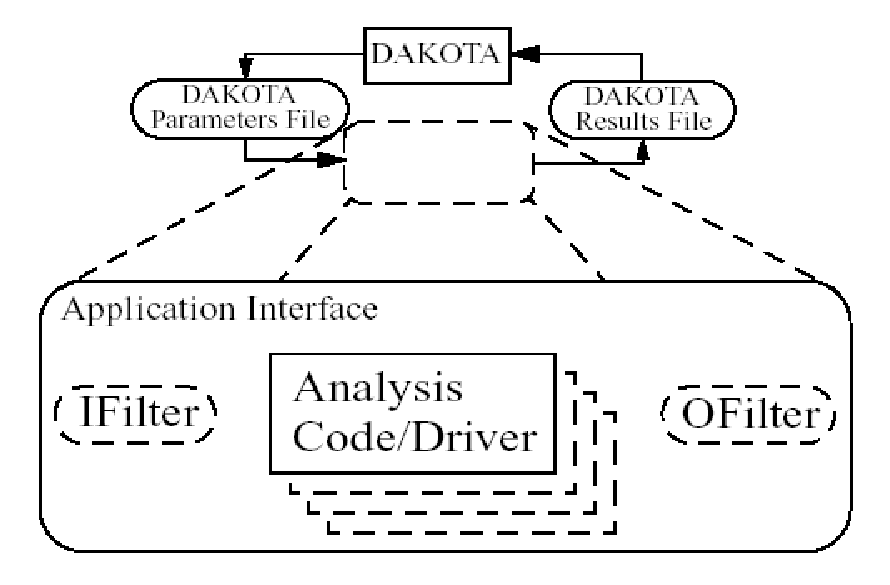
\includegraphics[scale=0.8]{images/dakota_components}
  \caption{Components of the simulation interface}
  \label{interfaces:bbinterfacecomp}
\end{figure}

When spawning function evaluations using system calls or forks, Dakota
must communicate parameter and response data with the analysis drivers
and filters through use of the file system. This is accomplished by
passing the names of the parameters and results files on the command
line when executing an analysis driver or filter. The input filter or
analysis driver read data from the parameters file and the output
filter or analysis driver write the appropriate data to the responses
file. While not essential when the file names are fixed, the file
names must be retrieved from the command line when Dakota is changing
the file names from one function evaluation to the next (i.e., using
temporary files or root names tagged with numerical identifiers).
In the case of a UNIX C-shell script, the two command line arguments
are retrieved using \texttt{\$argv[1]} and \texttt{\$argv[2]}
(see~\cite{And86}).  Similarly, Bourne shell scripts retrieve the two
command line arguments using \texttt{\$1} and \texttt{\$2}, and Perl
scripts retrieve the two command line arguments using
\texttt{@ARGV[0]} and \texttt{@ARGV[1]}.  In the case of a C or C++
program, command line arguments are retrieved using \texttt{argc}
(argument count) and \texttt{argv} (argument vector)~\cite{Ker88}, and
for Fortran 77, the \texttt{iargc} function returns the argument count
and the \texttt{getarg} subroutine returns command line arguments.

\subsection{Single analysis driver without filters}\label{interfaces:components:single1}

If a single \texttt{analysis\_driver} is selected in the interface
specification and filters are not needed (as indicated by omission of
the \texttt{input\_filter} and \texttt{output\_filter}
specifications), then only one process will appear in the execution
syntax of the simulation interface. An example of this syntax in the
system call case is:
\begin{small}
\begin{verbatim}
    driver params.in results.out
\end{verbatim}
\end{small}

where ``\texttt{driver}'' is the user-specified analysis driver and
``\texttt{params.in}'' and ``\texttt{results.out}'' are the names of the
parameters and results files, respectively, passed on the command
line. In this case, the user need not retrieve the command line
arguments since the same file names will be used each time.

For the same mapping, the fork simulation interface echoes the
following syntax:
\begin{small}
\begin{verbatim}
    blocking fork: driver params.in results.out
\end{verbatim}
\end{small}

for which only a single blocking fork is needed to perform the
evaluation.

Executing the same mapping with the direct simulation interface
results in an echo of the following syntax:
\begin{small}
\begin{verbatim}
    Direct function: invoking driver
\end{verbatim}
\end{small}

where this analysis driver must be linked as a function within
Dakota's direct interface (see Section~\ref{advint:direct}). Note that
no parameter or response files are involved, since such values
are passed directly through the function argument lists.

Both the system call and fork interfaces support asynchronous
operations. The asynchronous system call execution syntax involves
executing the system call in the background:
\begin{small}
\begin{verbatim}
    driver params.in.1 results.out.1 &
\end{verbatim}
\end{small}

and the asynchronous fork execution syntax involves use of a
nonblocking fork:
\begin{small}
\begin{verbatim}
    nonblocking fork: driver params.in.1 results.out.1
\end{verbatim}
\end{small}

where file tagging (see Section~\ref{interfaces:file:tagging1}) has
been user-specified in both cases to prevent conflicts between
concurrent analysis drivers. In these cases, the user must retrieve
the command line arguments since the file names change on each
evaluation.  Execution of the direct interface must currently be
performed synchronously since multithreading is not yet supported
(see Section~\ref{parallel:SLP:local:direct}).

\subsection{Single analysis driver with filters}\label{interfaces:components:single2}

When filters are used, the syntax of the system call that Dakota
performs is:
\begin{small}
\begin{verbatim}
    ifilter params.in results.out; driver params.in results.out;
         ofilter params.in results.out
\end{verbatim}
\end{small}

in which the input filter (``\texttt{ifilter}''), analysis driver
(``\texttt{driver}''), and output filter (``\texttt{ofilter}'')
processes are combined into a single system call through the use of
semi-colons (see~\cite{And86}). All three portions are
passed the names of the parameters and results files on the command
line.

For the same mapping, the fork simulation interface echoes the
following syntax:
\begin{small}
\begin{verbatim}
    blocking fork: ifilter params.in results.out;
         driver params.in results.out; ofilter params.in results.out
\end{verbatim}
\end{small}

where a series of three blocking forks is used to perform the
evaluation.

Executing the same mapping with the direct simulation interface
results in an echo of the following syntax:
\begin{small}
\begin{verbatim}
    Direct function: invoking { ifilter driver ofilter }
\end{verbatim}
\end{small}

where each of the three components must be linked as a function within
Dakota's direct interface. Since asynchronous operations are not yet
supported, execution simply involves invocation of each of the three
linked functions in succession. Again, no files are involved since
parameter and response data are passed directly through the function
argument lists.

Asynchronous executions would appear as follows for the system call
interface:
\begin{small}
\begin{verbatim}
    (ifilter params.in.1 results.out.1; driver params.in.1 results.out.1;
         ofilter params.in.1 results.out.1) &
\end{verbatim}
\end{small}

and, for the fork interface, as:
\begin{small}
\begin{verbatim}
    nonblocking fork: ifilter params.in.1 results.out.1;
         driver params.in.1 results.out.1; ofilter params.in.1 results.out.1
\end{verbatim}
\end{small}

where file tagging of evaluations has again been user-specified in
both cases. For the system call simulation interface, use of
parentheses and semi-colons to bind the three processes into a single
system call simplifies asynchronous process management compared to an
approach using separate system calls. The fork simulation interface,
on the other hand, does not rely on parentheses and accomplishes
asynchronous operations by first forking an intermediate process. This
intermediate process is then reforked for the execution of the input
filter, analysis driver, and output filter. The intermediate process
can be blocking or nonblocking (nonblocking in this case), and the
second level of forks can be blocking or nonblocking (blocking in this
case). The fact that forks can be reforked multiple times using either
blocking or nonblocking approaches provides the enhanced flexibility
to support a variety of local parallelism approaches (see
Chapter~\ref{parallel}).

\subsection{Multiple analysis drivers without filters}\label{interfaces:components:multiple1}

If a list of \texttt{analysis\_drivers} is specified and filters are
not needed (i.e., neither \texttt{input\_filter} nor
\texttt{output\_filter} appears), then the system call syntax
would appear as:
\begin{small}
\begin{verbatim}
    driver1 params.in results.out.1; driver2 params.in results.out.2;
         driver3 params.in results.out.3
\end{verbatim}
\end{small}

where ``\texttt{driver1}'', ``\texttt{driver2}'', and
``\texttt{driver3}'' are the user-specified analysis drivers and
``\texttt{params.in}'' and ``\texttt{results.out}'' are the
user-selected names of the parameters and results files. Note that the
results files for the different analysis drivers have been
automatically tagged to prevent overwriting. This automatic tagging of
\emph{analyses} (see Section~\ref{interfaces:file:tagging2}) is a
separate operation from user-selected tagging of \emph{evaluations}
(see Section~\ref{interfaces:file:tagging1}).

For the same mapping, the fork simulation interface echoes the
following syntax:
\begin{small}
\begin{verbatim}
    blocking fork: driver1 params.in results.out.1;
         driver2 params.in results.out.2; driver3 params.in results.out.3
\end{verbatim}
\end{small}

for which a series of three blocking forks is needed (no reforking of
an intermediate process is required).

Executing the same mapping with the direct simulation interface
results in an echo of the following syntax:
\begin{small}
\begin{verbatim}
    Direct function: invoking { driver1 driver2 driver3 }
\end{verbatim}
\end{small}

where, again, each of these components must be linked within Dakota's
direct interface and no files are involved for parameter and response
data transfer.

Both the system call and fork interfaces support asynchronous function
evaluations. The asynchronous system call execution syntax would be
reported as
\begin{small}
\begin{verbatim}
    (driver1 params.in.1 results.out.1.1; driver2 params.in.1 results.out.1.2;
         driver3 params.in.1 results.out.1.3) &
\end{verbatim}
\end{small}

and the nonblocking fork execution syntax would be reported as
\begin{small}
\begin{verbatim}
    nonblocking fork: driver1 params.in.1 results.out.1.1;
         driver2 params.in.1 results.out.1.2; driver3 params.in.1 results.out.1.3
\end{verbatim}
\end{small}

where, in both cases, file tagging of evaluations has been
user-specified to prevent conflicts between concurrent analysis
drivers and file tagging of the results files for multiple analyses is
automatically used. In the fork interface case, an intermediate
process is forked to allow a non-blocking function evaluation, and
this intermediate process is then reforked for the execution of each
of the analysis drivers.

\subsection{Multiple analysis drivers with filters}\label{interfaces:components:multiple2}

Finally, when combining filters with multiple
\texttt{analysis\_drivers}, the syntax of the system call that Dakota
performs is:
\begin{small}
\begin{verbatim}
    ifilter params.in.1 results.out.1;
         driver1 params.in.1 results.out.1.1;
         driver2 params.in.1 results.out.1.2;
         driver3 params.in.1 results.out.1.3;
         ofilter params.in.1 results.out.1
\end{verbatim}
\end{small}

in which all processes have again been combined into a single system
call through the use of semi-colons and parentheses. Note that the
secondary file tagging for the results files is only used for the
analysis drivers and not for the filters. This is consistent with the
filters' defined purpose of managing the non-repeated portions of
analysis pre- and post-processing (e.g., overlay of response results
from individual analyses; see Section~\ref{interfaces:file:tagging2}
for additional information).

For the same mapping, the fork simulation interface echoes the
following syntax:
\begin{small}
\begin{verbatim}
    blocking fork: ifilter params.in.1 results.out.1;
         driver1 params.in.1 results.out.1.1;
         driver2 params.in.1 results.out.1.2;
         driver3 params.in.1 results.out.1.3;
         ofilter params.in.1 results.out.1
\end{verbatim}
\end{small}

for which a series of five blocking forks is used (no reforking of an
intermediate process is required).

Executing the same mapping with the direct simulation interface
results in an echo of the following syntax:
\begin{small}
\begin{verbatim}
    Direct function: invoking { ifilter driver1 driver2 driver3 ofilter }
\end{verbatim}
\end{small}

where each of these components must be linked as a function within
Dakota's direct interface. Since asynchronous operations are not
supported, execution simply involves invocation of each of the five
linked functions in succession. Again, no files are involved for
parameter and response data transfer since this data is passed
directly through the function argument lists.

Asynchronous executions would appear as follows for the system call
interface:
\begin{small}
\begin{verbatim}
    (ifilter params.in.1 results.out.1;
         driver1 params.in.1 results.out.1.1;
         driver2 params.in.1 results.out.1.2;
         driver3 params.in.1 results.out.1.3;
         ofilter params.in.1 results.out.1) &
\end{verbatim}
\end{small}

and for the fork interface:
\begin{small}
\begin{verbatim}
    nonblocking fork: ifilter params.in.1 results.out.1;
         driver1 params.in.1 results.out.1.1;
         driver2 params.in.1 results.out.1.2;
         driver3 params.in.1 results.out.1.3;
         ofilter params.in.1 results.out.1
\end{verbatim}
\end{small}

where, again, user-selected file tagging of evaluations is combined
with automatic file tagging of analyses. In the fork interface case,
an intermediate process is forked to allow a non-blocking function
evaluation, and this intermediate process is then reforked for the
execution of the input filter, each of the analysis drivers, and the
output filter.

A complete example of these filters and multi-part drivers can be
found in \texttt{Dakota/test/dakota\_3pc/dakota\_3pc.in}.

\section{Simulation File Management}\label{interfaces:file}

This section describes some management features used for files that
transfer data between Dakota and simulation codes
(i.e., when the system call or fork interfaces are used). These
features can generate unique filenames when
Dakota executes programs in parallel and can help one debug
the interface between Dakota and a simulation code.

\subsection{File Saving}\label{interfaces:file:saving}

{\bf Before driver execution:} In Dakota 5.0 and newer, an existing
results file will be removed immediately prior to executing the
analysis driver.  This new behavior addresses a common user problem
resulting from starting Dakota with stale results files in the run
directory.  To override this default behavior and preserve any
existing results files, specify \texttt{allow\_existing\_results}.

{\bf After driver execution:} The \texttt{file\_save} option in the
interface specification allows the user to control whether parameters
and results files are retained or removed from the working directory
after the analysis completes. Dakota's default behavior is to remove
files once their use is complete to reduce clutter. If the method
output setting is verbose, a file remove notification will follow the
function evaluation echo, e.g.,
\begin{small}
\begin{verbatim}
    driver /usr/tmp/aaaa20305 /usr/tmp/baaa20305
    Removing /usr/tmp/aaaa20305 and /usr/tmp/baaa20305
\end{verbatim}
\end{small}

However, if \texttt{file\_save} appears in the interface
specification, these files will not be removed. This latter behavior
is often useful for debugging communication between Dakota and
simulator programs. An example of a \texttt{file\_save} specification
is shown in the file tagging example below.

\subsection{File Tagging for Evaluations}\label{interfaces:file:tagging1}

When a user provides \texttt{parameters\_file} and
\texttt{results\_file} specifications, the \texttt{file\_tag} option
in the interface specification causes Dakota to make the names of
these files unique by appending the function
evaluation number to the root file names. Default behavior is to not
tag these files, which has the advantage of allowing the user to
ignore command line argument passing and always read to and write from
the same file names. However, it has the disadvantage that files may
be overwritten from one function evaluation to the next. When
\texttt{file\_tag} appears in the interface specification, the file names
are made unique by the appended evaluation number. This uniqueness
requires the user's interface to get the names of
these files from the command line. The file tagging feature is most
often used when concurrent simulations are running in a common disk
space, since it can prevent conflicts between the simulations. An
example specification of \texttt{file\_tag} and \texttt{file\_save} is
shown below:
\begin{small}
\begin{verbatim}
    interface,
            system
              analysis_driver = 'text_book'
              parameters_file = 'text_book.in'
              results_file    = 'text_book.out'
              file_tag file_save
\end{verbatim}
\end{small}

\emph{Special case:} When a user specifies names for the parameters
and results files and \texttt{file\_save} is used without
\texttt{file\_tag}, untagged files are used in the function evaluation
but are then moved to tagged files after the function evaluation is
complete, to prevent overwriting files for which a
\texttt{file\_save} request has been given. If the output control is
set to verbose, then a notification similar to the following will
follow the function evaluation echo:
\begin{small}
\begin{verbatim}
    driver params.in results.out
    Files with non-unique names will be tagged to enable file_save:
    Moving params.in to params.in.1
    Moving results.out to results.out.1
\end{verbatim}
\end{small}

\textbf{Hierarchical tagging:} When a model's specification includes
the {\tt hierarchical\_tagging} keyword, the tag applied to parameter
and results file names of any subordinate interfaces will reflect any
model hierarchy present.  This option is useful for studies involving
multiple models with a nested or hierarchical relationship.  For
example a nested model has a sub-method, which itself likely operates
on a sub-model, or a hierarchical approximation involves coordination
of low and high fidelity models.  Specifying {\tt
  hierarchical\_tagging} will yield function evaluation identifiers
(``tags'') composed of the evaluation IDs of the models involved,
e.g., outermodel.innermodel.interfaceid = 4.9.2.  This communicates
the outer contexts to the analysis driver when performing a function
evaluation.  For an example of using hierarhical tagging in a nested
model context, see {\tt
  dakota/test/dakota\_uq\_timeseries\_*\_optinterf.in}.

\subsection{Temporary Files}\label{interfaces:file:temporary}

If \texttt{parameters\_file} and \texttt{results\_file} are not
specified by the user, temporary files having generated names are
used.  For example, a system call to a single analysis driver might
appear as:
\begin{small}
\begin{verbatim}
    driver /tmp/dakota_params_aaaa2035 /tmp/dakota_results_baaa2030
\end{verbatim}
\end{small}

and a system call to an analysis driver with filter programs might appear as:
\begin{small}
\begin{verbatim}
    ifilter /tmp/dakota_params_aaaa2490 /tmp/dakota_results_baaa2490;
         driver /tmp/dakota_params_aaaa2490 tmp/dakota_results_baaa2490;
         ofilter /tmp/dakota_params_aaaa2490 /tmp/dakota_results_baa22490
\end{verbatim}
\end{small}

These files have unique names created by Boost filesystem
utilities. This uniqueness requires the user's interface to get the
names of these files from the command line. File tagging with
evaluation number is unnecessary with temporary files, but can be
helpful for the user workflow to identify the evaluation number.  Thus
\texttt{file\_tag} requests will be honored. A \texttt{file\_save}
request will be honored, but it should be used with care since the
temporary file directory could easily become cluttered without the
user noticing.

\subsection{File Tagging for Analysis Drivers}\label{interfaces:file:tagging2}

When multiple analysis drivers are involved in performing a function
evaluation with either the system call or fork simulation interface,
a secondary file tagging is \emph{automatically} used to
distinguish the results files used for the individual analyses. This
applies to both the case of user-specified names for the parameters
and results files and the default temporary file case. Examples
for the former case were shown previously in
Section~\ref{interfaces:components:multiple1} and
Section~\ref{interfaces:components:multiple2}.  The following examples
demonstrate the latter temporary file case. Even though Unix
temporary files have unique names for a particular function
evaluation, tagging is still needed to manage the individual
contributions of the different analysis drivers to the response
results, since the same root results filename is used for each
component. For the system call interface, the syntax would be similar
to the following:
\begin{small}
\begin{verbatim}
    ifilter /var/tmp/aaawkaOKZ /var/tmp/baaxkaOKZ;
         driver1 /var/tmp/aaawkaOKZ /var/tmp/baaxkaOKZ.1;
         driver2 /var/tmp/aaawkaOKZ /var/tmp/baaxkaOKZ.2;
         driver3 /var/tmp/aaawkaOKZ /var/tmp/baaxkaOKZ.3;
         ofilter /var/tmp/aaawkaOKZ /var/tmp/baaxkaOKZ
\end{verbatim}
\end{small}

and, for the fork interface, similar to:
\begin{small}
\begin{verbatim}
    blocking fork:
         ifilter /var/tmp/aaawkaOKZ /var/tmp/baaxkaOKZ;
         driver1 /var/tmp/aaawkaOKZ /var/tmp/baaxkaOKZ.1;
         driver2 /var/tmp/aaawkaOKZ /var/tmp/baaxkaOKZ.2;
         driver3 /var/tmp/aaawkaOKZ /var/tmp/baaxkaOKZ.3;
         ofilter /var/tmp/aaawkaOKZ /var/tmp/baaxkaOKZ
\end{verbatim}
\end{small}

Tagging of results files with an analysis identifier is needed
since each analysis driver must contribute a
user-defined subset of the total response results for the evaluation.
If an output filter is not supplied, Dakota will combine these
portions through a simple overlaying of the individual contributions
(i.e., summing the results in \texttt{/var/tmp/baaxkaOKZ.1},
\texttt{/var/tmp/baaxkaOKZ.2}, and \texttt{/var/tmp/baaxkaOKZ.3}). If
this simple approach is inadequate, then an output filter should be
supplied to perform the combination. This is the reason why the
results file for the output filter does not use analysis tagging; it
is responsible for the results combination (i.e., combining
\texttt{/var/tmp/baaxkaOKZ.1}, \texttt{/var/tmp/baaxkaOKZ.2}, and
\texttt{/var/tmp/baaxkaOKZ.3} into \texttt{/var/tmp/baaxkaOKZ}). In
this case, Dakota will read only the results file from the output
filter (i.e., \texttt{/var/tmp/baaxkaOKZ}) and interpret it as the
total response set for the evaluation.

Parameters files are not currently tagged with an analysis identifier.
This reflects the fact that Dakota does not attempt to subdivide the
requests in the active set vector for different analysis portions.
Rather, the total active set vector is passed to each analysis driver
and the appropriate subdivision of work \emph{must be defined by the
  user}. This allows the division of labor to be very flexible. In
some cases, this division might occur across response functions, with
different analysis drivers managing the data requests for different
response functions. And in other cases, the subdivision might occur
within response functions, with different analysis drivers
contributing portions to each of the response functions. The only
restriction is that each of the analysis drivers must follow the
response format dictated by the total active set vector. For response
data for which an analysis driver has no contribution, 0's must be
used as placeholders.

\subsection{Work Directories}\label{interfaces:workdir}

Sometimes it is convenient for simulators and filters to run in a
directory different from the one where Dakota is invoked.  For instance,
when performing concurrent evaluations and/or analyses, it is often
necessary to cloister input and output files in separate directories to
avoid conflicts.  A simulator script used as an \texttt{analysis\_driver}
can of course include commands to change to a different directory if
desired (while still arranging to write a results file in the original
directory), but Dakota has facilities that may simplify the creation of
simulator scripts.  When the \texttt{work\_directory} feature is enabled,
Dakota will create a directory for each evaluation/analysis (with
optional tagging and saving as with files).  To enable the
\texttt{work\_directory} feature an interface specification includes
the keyword
\begin{small}
\begin{verbatim}
       work_directory
\end{verbatim}
\end{small}
then Dakota will arrange for the simulator and any filters to
wake up in the work directory, with \$PATH adjusted (if necessary)
so programs that could be invoked without a relative
path to them (i.e., by a name not involving any slashes) from
Dakota's directory can also be invoked from the simulator's (and filter's)
directory.  On occasion, it is convenient for the simulator to have
various files, e.g., data files, available in the directory where it
runs.  If, say, \texttt{my/special/directory} is such a directory
(as seen from Dakota's directory), the interface specification
\begin{small}
\begin{verbatim}
       work_directory named 'my/special/directory'
\end{verbatim}
\end{small}
would cause Dakota to start the simulator and any filters in that
directory.  If the directory did not already exist, Dakota would
create it and would remove it after the simulator (or output filter,
if specifed) finished, unless instructed not to do so by the
appearance of \texttt{directory\_save} (or its deprecated synonym
\texttt{dir\_save}) in the interface specification.  If \texttt{named
  '$...$'} does not appear, then \texttt{directory\_save} cannot
appear either, and Dakota creates a temporary directory (using the
\texttt{tmpnam} function to determine its name) for use by the
simulator and any filters.  If you specify \texttt{directory\_tag} (or
the deprecated \texttt{dir\_tag}), Dakota causes each invocation of
the simulator and any filters to start in a a subdirectory of the work
directory with a name composed of the work directory's name followed
by a period and the invocation number (1, 2, $...$); this might be
useful in debugging.

Sometimes it can be helpful for the simulator and filters to start in a
new directory populated with some files.  Adding
\begin{small}
\begin{verbatim}
       link_files 'templatedir/*'
\end{verbatim}
\end{small}
to the work directory specification would cause the
contents of directory \texttt{templatedir} to be linked
into the work directory.  Linking makes sense if files are large,
but when practical, it is far more reliable to have
copies of the files; adding \texttt{copy\_files} to the specification
would cause the contents of the template directory to be copied
to the work directory.  The linking or copying does
not overwrite existing files unless \texttt{replace} also appears
in the specification.

Here is a summary of possibilities for a work directory specification,
with {\tt\verb=[=$...$\verb=]=} denoting that $...$ is optional:
\begin{small}
\begin{verbatim}
  work_directory [ named '...' ]
    [ directory_tag ]     # (or dir_tag)
    [ directory_save ]    # (or dir_save)
    [ link_files '...' '...' ]
    [ copy_files '...' '...' ]
    [ replace ]
\end{verbatim}
\end{small}

\section{Parameter to Response Mapping Examples}\label{interfaces:mappings}

In this section, interface mapping examples are presented through the
discussion of several parameters files and their corresponding results
files. A typical input file for 2 variables ($n=2$) and 3 functions
($m=3$) using the standard parameters file format (see
Section~\ref{variables:parameters:standard}) is as follows:
\begin{small}
\begin{verbatim}
                        2 variables
    1.500000000000000e+00 cdv_1
    1.500000000000000e+00 cdv_2
                        3 functions
                        1 ASV_1
                        1 ASV_2
                        1 ASV_3
                        2 derivative_variables
                        1 DVV_1
                        2 DVV_2
                        0 analysis_components
\end{verbatim}
\end{small}
where numerical values are associated with their tags within
``\texttt{value tag}'' constructs. The number of design variables
($n$) and the string ``\texttt{variables}'' are followed by the values
of the design variables and their tags, the number of functions ($m$)
and the string ``\texttt{functions}'', the active set vector (ASV) and
its tags, the number of derivative variables and the string
``\texttt{derivative\_variables}'', the derivative variables vector
(DVV) and its tags, the number of analysis components and the string
``\texttt{analysis\_components}'', and the analysis components array
and its tags.  The descriptive tags for the variables are always
present and they are either the descriptors in the user's variables
specification, if given there, or are default descriptors.  The length
of the active set vector is equal to the number
of functions ($m$). In the case of an optimization data set with an
objective function and two nonlinear constraints (three response
functions total), the first ASV value is associated with the objective
function and the remaining two are associated with the constraints (in
whatever consistent constraint order has been defined by the user).
The DVV defines a subset of the variables used for computing
derivatives.  Its identifiers are 1-based and correspond to the full
set of variables listed in the first array.  Finally, the analysis
components pass additional strings from the user's
\texttt{analysis\_components} specification in a Dakota input file
through to the simulator.  They allow the development of simulation
drivers that are more flexible, by allowing them to be passed
additional specifics at run time, e.g., the names of model files such
as a particular mesh to use.

For the APREPRO format option (see
Section~\ref{variables:parameters:aprepro}), the same set of data
appears as follows:
\begin{small}
\begin{verbatim}
    { DAKOTA_VARS     =                      2 }
    { cdv_1           =  1.500000000000000e+00 }
    { cdv_2           =  1.500000000000000e+00 }
    { DAKOTA_FNS      =                      3 }
    { ASV_1           =                      1 }
    { ASV_2           =                      1 }
    { ASV_3           =                      1 }
    { DAKOTA_DER_VARS =                      2 }
    { DVV_1           =                      1 }
    { DVV_2           =                      2 }
    { DAKOTA_AN_COMPS =                      0 }
\end{verbatim}
\end{small}

where the numerical values are associated with their tags within
``\texttt{\{ tag = value \}}'' constructs.

The user-supplied simulation interface, comprised of a simulator
program or driver and (optionally) filter programs, is responsible for
reading the parameters file and creating a results file that contains
the response data requested in the ASV. This response data is written
in the format described in Section~\ref{responses:results}. Since the
ASV contains all ones in this case, the response file corresponding to
the above input file would contain values for the three functions:
\begin{small}
\begin{verbatim}
    1.250000000000000e-01 f
    1.500000000000000e+00 c1
    1.500000000000000e+00 c2
\end{verbatim}
\end{small}

Since function tags are optional, the following would be equally
acceptable:
\begin{small}
\begin{verbatim}
    1.250000000000000e-01
    1.500000000000000e+00
    1.500000000000000e+00
\end{verbatim}
\end{small}

For the same parameters with different ASV components,
\begin{small}
\begin{verbatim}
                        2 variables
    1.500000000000000e+00 cdv_1
    1.500000000000000e+00 cdv_2
                        3 functions
                        3 ASV_1
                        3 ASV_2
                        3 ASV_3
                        2 derivative_variables
                        1 DVV_1
                        2 DVV_2
                        0 analysis_components
\end{verbatim}
\end{small}

the following response data is required:
\begin{small}
\begin{verbatim}
    1.250000000000000e-01 f
    1.500000000000000e+00 c1
    1.500000000000000e+00 c2
    [ 5.000000000000000e-01 5.000000000000000e-01 ]
    [ 3.000000000000000e+00 -5.000000000000000e-01 ]
    [ -5.000000000000000e-01 3.000000000000000e+00 ]
\end{verbatim}
\end{small}
Here, we need not only the function values, but also each of their
gradients. The derivatives are computed with respect to \texttt{cdv\_1}
and \texttt{cdv\_2} as indicated by the DVV values. Another modification
to the ASV components yields the following parameters file:
\begin{small}
\begin{verbatim}
                        2 variables
    1.500000000000000e+00 cdv_1
    1.500000000000000e+00 cdv_2
                        3 functions
                        2 ASV_1
                        0 ASV_2
                        2 ASV_3
                        2 derivative_variables
                        1 DVV_1
                        2 DVV_2
                        0 analysis_components
\end{verbatim}
\end{small}

for which the following results file is needed:
\begin{small}
\begin{verbatim}
    [ 5.000000000000000e-01 5.000000000000000e-01 ]
    [ -5.000000000000000e-01 3.000000000000000e+00 ]
\end{verbatim}
\end{small}
Here, we need gradients for functions \texttt{f} and \texttt{c2}, but
not for \texttt{c1}, presumably since this constraint is inactive.

A full Newton optimizer might make the following request:
\begin{small}
\begin{verbatim}
                        2 variables
    1.500000000000000e+00 cdv_1
    1.500000000000000e+00 cdv_2
                        1 functions
                        7 ASV_1
                        2 derivative_variables
                        1 DVV_1
                        2 DVV_2
                        0 analysis_components
\end{verbatim}
\end{small}

for which the following results file,
\begin{small}
\begin{verbatim}
    1.250000000000000e-01 f
    [ 5.000000000000000e-01 5.000000000000000e-01 ]
    [[ 3.000000000000000e+00 0.000000000000000e+00
       0.000000000000000e+00 3.000000000000000e+00 ]]
\end{verbatim}
\end{small}
containing the objective function, its gradient vector, and its
Hessian matrix, is needed.  Again, the derivatives (gradient vector
and Hessian matrix) are computed with respect to \texttt{cdv\_1} and
\texttt{cdv\_2} as indicated by the DVV values.

Lastly, a more advanced example could have multiple types of variables
present; in this example, 2 continuous design and 3 discrete design
range, 2 normal uncertain, and 3 continuous state and 2 discrete state
range variables.  When a mixture of variable types is present, the
content of the DVV (and therefore the required length of gradient
vectors and Hessian matrices) depends upon the type of study being
performed (see Section~\ref{responses:active}).  For a reliability
analysis problem, the uncertain variables are the active continuous
variables and the following parameters file would be typical:
\begin{small}
\begin{verbatim}
                       12 variables
    1.500000000000000e+00 cdv_1
    1.500000000000000e+00 cdv_2
                        2 ddriv_1
                        2 ddriv_2
                        2 ddriv_3
    5.000000000000000e+00 nuv_1
    5.000000000000000e+00 nuv_2
    3.500000000000000e+00 csv_1
    3.500000000000000e+00 csv_2
    3.500000000000000e+00 csv_3
                        4 dsriv_1
                        4 dsriv_2
                        3 functions
                        3 ASV_1
                        3 ASV_2
                        3 ASV_3
                        2 derivative_variables
                        6 DVV_1
                        7 DVV_2
                        2 analysis_components
                mesh1.exo AC_1
                  db1.xml AC_2
\end{verbatim}
\end{small}

Gradients are requested with respect to variable entries 6 and 7,
which correspond to normal uncertain variables \texttt{nuv\_1} and
\texttt{nuv\_2}.  The following response data would be appropriate:
\begin{small}
\begin{verbatim}
    7.943125000000000e+02 f
    1.500000000000000e+00 c1
    1.500000000000000e+00 c2
    [ 2.560000000000000e+02 2.560000000000000e+02 ]
    [ 0.000000000000000e+00 0.000000000000000e+00 ]
    [ 0.000000000000000e+00 0.000000000000000e+00 ]
\end{verbatim}
\end{small}

In a parameter study, however, no distinction is drawn between
different types of continuous variables, and derivatives would be
needed with respect to all continuous variables ($n_{dvv}=7$ for the
continuous design variables \texttt{cdv\_1} and \texttt{cdv\_2}, the
normal uncertain variables \texttt{nuv\_1} and \texttt{nuv\_2}, and
the continuous state variables \texttt{csv\_1}, \texttt{csv\_2} and
\texttt{csv\_3}).  The parameters file would appear as
\begin{small}
\begin{verbatim}
                       12 variables
    1.500000000000000e+00 cdv_1
    1.500000000000000e+00 cdv_2
                        2 ddriv_1
                        2 ddriv_2
                        2 ddriv_3
    5.000000000000000e+00 nuv_1
    5.000000000000000e+00 nuv_2
    3.500000000000000e+00 csv_1
    3.500000000000000e+00 csv_2
    3.500000000000000e+00 csv_3
                        4 dsriv_1
                        4 dsriv_2
                        3 functions
                        3 ASV_1
                        3 ASV_2
                        3 ASV_3
                        7 derivative_variables
                        1 DVV_1
                        2 DVV_2
                        6 DVV_3
                        7 DVV_4
                        8 DVV_5
                        9 DVV_6
                       10 DVV_7
                        2 analysis_components
                mesh1.exo AC_1
                  db1.xml AC_2
\end{verbatim}
\end{small}

and the corresponding results would appear as
\begin{small}
\begin{verbatim}
    7.943125000000000e+02 f
    1.500000000000000e+00 c1
    1.500000000000000e+00 c2
    [  5.000000000000000e-01  5.000000000000000e-01  2.560000000000000e+02
       2.560000000000000e+02  6.250000000000000e+01  6.250000000000000e+01
       6.250000000000000e+01 ]
    [  3.000000000000000e+00 -5.000000000000000e-01  0.000000000000000e+00
       0.000000000000000e+00  0.000000000000000e+00  0.000000000000000e+00
       0.000000000000000e+00 ]
    [ -5.000000000000000e-01  3.000000000000000e+00  0.000000000000000e+00
       0.000000000000000e+00  0.000000000000000e+00  0.000000000000000e+00
       0.000000000000000e+00 ]
\end{verbatim}
\end{small}

\section{Parameters and Results Files with dakota.interfacing}\label{interfaces:dakota.interfacing}

The Python module {\tt dakota.interfacing} first was made available with Dakota 6.6. (It was released with Dakota 6.5 as the module {\tt dipy}.) By providing a Python interface to read and write, respectively, Dakota parameters and results files, {\tt dakota.interfacing} can greatly simplify development of black-box interfaces. The benefit may be greatest when one or more phases of the interface (pre-processing, execution, post-processing) is written in Python.

The following sections describe the components of {\tt dakota.interfacing}. These include a {\tt Parameters} class for making variable information available, a {\tt Results} class for collecting results and writing them to file, and a convenience function {\tt read\_parameters\_file}, the preferred way to construct {\tt Parameters} and {\tt Results} objects from a Dakota parameters file.

\subsection{Creating Parameters and Results objects}

{\tt dakota.interfacing} has one free function, {\tt read\_parameters\_file}, which creates {\tt Parameters} and {\tt Results} objects based on a Dakota parameters file. Its signature is:

\phantomsection\label{index:dakota.interfacing.read_parameters_file}\texttt{dakota.interfacing.}\textbf{\texttt{read\_parameters\_file}}({\emph{parameters\_file=None}, \emph{results\_file=None}, \emph{ignore\_asv=False}}){}

\emph{parameters\_file} and \emph{results\_file} are the names of the parameters file that is to be read and the results file that  ultimately is to be written. The names can be  absolute or relative filepaths or just filenames. If a parameters file or results file is not provided, it will be obtained from the command line arguments. (The results filename is assumed to be the last command line argument, and the parameters file the second to last.) Note that if the working directory has changed since script invocation, filenames provided as command line arguments by Dakota's {\tt fork} or {\tt system} interfaces may be incorrect.

If \emph{results\_file} is set to the constant {\tt dakota.interfacing.UNNAMED}, the {\tt Results} object is constructed without a results file name.  In this case, an output stream must be provided when {\tt Results.write()} is called. Unnamed results files are most helpful when no results file will be written, as with a script intended purely for pre-processing.

By default, the returned {\tt Results} object enforces the active set vector (see the {\tt Results} class section). This behavior can be overriden, allowing any property (function, gradient, Hessian) of a response to be set, by setting \emph{ignore\_asv} to True.


\subsection{Parameters objects}

{\tt Parameters} objects make the variables, analysis components, evaluation ID, and evaluation number read from a Dakota parameters file available through a combination of key-value access and object attributes. Although {\tt Parameters} objects may be constructed directly, it is advisable to use the {\tt read\_parameters\_file} function instead.

Variable values can be accessed by Dakota descriptor or by index using {[}{]} on the object itself. Variables types (integer, real, string) are inferred by first attempting to convert to {\tt int} and then, if this fails, to {\tt float}.

Analysis components are accessible by index only using the {\tt an\_comps} attribute. {\tt Parameters} objects support iteration over the variables, yielding the index, variable descriptor, and variable value.

{\tt Parameters} objects have the attributes:

\begin{itemize}

  \item\index{an\_comps (dakota.interfacing.Parameters attribute)} \phantomsection\label{index:dakota.interfacing.Parameters.an_comps}\textbf{\texttt{an\_comps}} List of the analysis components (strings).

  \item\index{eval\_id (dakota.interfacing.Parameters attribute)} \phantomsection\label{index:dakota.interfacing.Parameters.eval_id}\textbf{\texttt{eval\_id}} Evaluation id (string).

  \item\index{eval\_num (dakota.interfacing.Parameters attribute)} \phantomsection\label{index:dakota.interfacing.Parameters.eval_num}\textbf{\texttt{eval\_num}} Evaluation number (final token in eval\_id) (int).


  \item\index{aprepro\_format (dakota.interfacing.Parameters attribute)} \phantomsection\label{index:dakota.interfacing.Parameters.aprepro_format}\textbf{\texttt{aprepro\_format}} Boolean indicating whether the parameters file was in aprepro (True) or Dakota (False) format.

  \item\index{descriptors (dakota.interfacing.Parameters attribute)}\phantomsection\label{index:dakota.interfacing.Parameters.descriptors}\textbf{\texttt{descriptors}} List of the variable descriptors

  \item\index{num\_variables (dakota.interfacing.Parameters attribute)} \phantomsection\label{index:dakota.interfacing.Parameters.num_variables}\textbf{\texttt{num\_variables}} Number of variables

  \item\index{num\_an\_comps (dakota.interfacing.Parameters attribute)}\phantomsection\label{index:dakota.interfacing.Parameters.num_an_comps}\textbf{\texttt{num\_an\_comps}} Number of analysis components

\end{itemize}

\subsection{Results objects}

{\tt Results} objects:
\begin{itemize}

  \item communicate response requests from Dakota (active set vector and derivative variables)
  \item collect response data (function values, gradients, and Hessians)
  \item write Dakota results files
\end{itemize}

{\tt Results} objects are collections of {\tt Response} objects, which are documented in the following section. Each {\tt Response} can be accessed by name (Dakota descriptor) or by index using {[}{]} on the {\tt Results} object itself. {\tt Results} objects support iteration of the {\tt Response}s, yielding the index, response descriptor, and {\tt Response}. Although {\tt Results} objects may be constructed directly, it is advisable to use the {\tt read\_parameters\_file} function instead.

Results objects have the attributes:

\begin{itemize}

  \item\index{eval\_id (dakota.interfacing.Results attribute)} \phantomsection\label{index:dakota.interfacing.Results.eval_id}\textbf{\texttt{eval\_id}} Evaluation id (a string).

  \item\index{eval\_num (dakota.interfacing.Results attribute)} \phantomsection\label{index:dakota.interfacing.Results.eval_num}\textbf{\texttt{eval\_num}} Evaluation number (final token in eval\_id) (int).

  \item\index{aprepro\_format (dakota.interfacing.Results attribute)} \phantomsection\label{index:dakota.interfacing.Results.aprepro_format}\textbf{\texttt{aprepro\_format}} Boolean indicating whether the parameters file was in
aprepro (True) or Dakota (False) format.

  \item\index{descriptors (dakota.interfacing.Results attribute)} \phantomsection\label{index:dakota.interfacing.Results.descriptors}\textbf{\texttt{descriptors}} List of the response descriptors (strings)

  \item\index{num\_responses (dakota.interfacing.Results attribute)}  \phantomsection\label{index:dakota.interfacing.Results.num_responses}\textbf{\texttt{num\_responses}} Number of variables (read-only)

  \item\index{deriv\_vars (dakota.interfacing.Results attribute)} \phantomsection\label{index:dakota.interfacing.Results.deriv_vars}\textbf{\texttt{deriv\_vars}} List of the derivative variables (strings)

  \item\index{num\_deriv\_vars (dakota.interfacing.Results attribute)}\phantomsection\label{index:dakota.interfacing.Results.num_deriv_vars}\textbf{\texttt{num\_deriv\_vars}}Number of derivative variables (int)

\end{itemize}

Results objects have the methods:

\begin{itemize}
  \item\index{fail() (dakota.interfacing.Results method)}
	  \phantomsection\label{index:dakota.interfacing.Results.fail}\textbf{\texttt{fail}}{()}{}
	  Set the FAIL attribute. When the results file is written, it will contain only the word FAIL, triggering Dakota's failure capturing behavior (See Chapter~\ref{failure}).

\item \index{write() (dakota.interfacing.Results method)}
	\phantomsection\label{index:dakota.interfacing.Results.write}\textbf{\texttt{write}}({\emph{stream=None}, \emph{ignore\_asv=None}}){}
Write the results to the Dakota results file. If \emph{stream} is set, it overrides the results file name provided at construct time. It must be an open file-like object, rather than the name of a file. If \emph{ignore\_asv} is True, the file will be written even if information requested via the active set vector is missing.

\end{itemize}

\subsection{Response object}

{\tt Response} objects store response information. They typically are instantiated and accessed through a Results object by index or response descriptor using {[}{]}.

{\tt Response}s have the attributes:

\begin{itemize}
  \item \index{asv (dakota.interfacing.Response attribute)} \phantomsection\label{index:dakota.interfacing.Response.asv}\textbf{\texttt{asv}} a {\tt collections.namedtuple} with three members, \emph{function}, \emph{gradient}, and \emph{hessian}.
Each is a boolean indicating whether Dakota requested the
associated information for the response. {\tt namedtuples} can be
accessed by index or by member.

  \item \index{function (dakota.interfacing.Response attribute)} \phantomsection\label{index:dakota.interfacing.Response.function}\textbf{\texttt{function}} Function value for the response. A ResponseError
is raised if Dakota did not request the function value (and
ignore\_asv is False).
  \item\index{gradient (dakota.interfacing.Response attribute)} \phantomsection\label{index:dakota.interfacing.Response.gradient}\textbf{\texttt{gradient}} Gradient for the response. Gradients must be a 1D iterable of values that can be converted to floats, such as a {\tt list} or 1D {\tt numpy array}. A ResponseError is raised if Dakota did not request the gradient (and ignore\_asv is False), or if the number of elements does not equal the number of derivative variables.

  \item \index{hessian (dakota.interfacing.Response attribute)} \phantomsection\label{index:dakota.interfacing.Response.hessian}\textbf{\texttt{hessian}} Hessian value for the response. Hessians must be an iterable of iterables (e.g. a 2D {\tt numpy array} or list of lists). A ResponseError is raised if Dakota did not request the Hessian (and ignore\_asv is False), or if the dimension does not correspond correctly with the number of derivative variables.

\end{itemize}

\subsection{dakota.interfacing Examples}

In addition to those in this section, the {\tt Dakota/examples/script\_interfaces/Python} folder contains two runnable examples of Python analysis drivers. In one, {\tt rosenbrock\_bb.py}, parameters file parsing is performed manually. The other, {\tt rosenbrock\_bb\_di.py}, demonstrates the {\tt dakota.interfacing} module.

For most applications, using {\tt dakota.interfacing} is straightforward. The first example, in Figure~\ref{diexample:simple}, is a mock analysis driver. Two variables with the descriptors {\tt x1} and {\tt x2} are read from the Dakota parameters file and used to evaluate the fictitious user function {\tt applic\_module.run()}. The result, stored in {\tt f}, is assigned to the {\tt function} value of the appropriate response. (A common error is leaving off the {\tt function} attribute, which is needed to distinguish the function value of the response from its gradient and Hessian.)

\begin{figure}
\begin{bigbox}
\begin{small}
\begin{verbatim}
  import dakota.interfacing as di
  import applic_module 

  params, results = di.read_parameters_file()

  # parameters can be accessed by descriptor, as shown here, or by index
  x1 = params["x1"]
  x2 = params["x2"]

  f = applic_module.run(x1,x2)

  # Responses also can be accessed by descriptor or index
  results["f"].function = f
  results.write()
\end{verbatim}
\end{small}
\end{bigbox}
\caption{A simple analysis driver that uses {\tt dakota.interfacing}}
\label{diexample:simple}
\end{figure}

The {\tt Results} object exposes the active set vector read from the parameters file. When analytic gradients or Hessians are available for a response, the ASV should be queried to determine what Dakota has requested for an evaluation. If an attempt is made to addunrequested information to a response, a {\tt dakota.interface.ResponseError} is raised. The same exception results if a requested piece of information is missing when {\tt Results.write()} is called. The \emph{ignore\_asv} option to {\tt read\_parameters\_file} and {\tt Results.write()} overrides ASV checks.

In Figure~\ref{diexample:asv}, {\tt applic\_module.run()} has been modified to return not only the function value of {\tt f}, but also its gradient and Hessian. The {\tt asv} attribute is examined to determine which of these to add to {\tt results["f"]}.

\begin{figure}
\begin{bigbox}
\begin{small}
\begin{verbatim}
  import dakota.interfacing as di
  import applic_module # fictitious application

  params, results = di.read_parameters_file()

  x1 = params["x1"]
  x2 = params["x2"]

  f, df, df2 = applic_module.run(x1,x2)

  if Results.asv.function:
      results["f"].function = f
  if Results.asv.gradient:
      results["f"].gradient = df
  if Results.asv.hessian:
      results["f"] = df2

  results.write()
\end{verbatim}


\end{small}
\end{bigbox}
\caption{Examining the active set vector}
\label{diexample:asv}
\end{figure}



\chapter{Responses}\label{responses}

\section{Overview}\label{responses:overview}

The \texttt{responses} specification in a DAKOTA input file controls
the types of data that can be returned from an interface during
DAKOTA's execution. The specification includes the number and type of
response functions (objective functions, nonlinear constraints, least
squares terms, etc.) as well as availability of first and second
derivatives (gradient vectors and Hessian matrices) for these response
functions.

This chapter will present a brief overview of the response data sets
and their uses, as well as cover some user issues relating to file
formats and derivative vector and matrix sizing. For a detailed
description of responses section syntax and example specifications,
refer to the Responses Commands chapter in the DAKOTA Reference
Manual~\cite{RefMan}.

\subsection{Response function types}\label{responses:overview:types}

The types of response functions listed in the responses
specification should be consistent with the
iterative technique called for in the method specification:

\begin{itemize}

\item an optimization data set comprised of
  \texttt{num\_objective\_functions},\\
  \texttt{num\_nonlinear\_inequality\_constraints}, and
  \texttt{num\_nonlinear\_equality\_constraints}.  This data set is
  appropriate for use with optimization methods (e.g., the methods in
  Section~\ref{capabilities:optimization1}).
  
\item a least squares data set comprised of 
  \texttt{num\_least\_squares\_terms},\\
  \texttt{num\_nonlinear\_inequality\_constraints}, and
  \texttt{num\_nonlinear\_equality\_constraints}.  This data set is
  appropriate for use with nonlinear least squares algorithms
  (e.g., the methods in Section~\ref{capabilities:nonlinear}).
  
\item a generic data set comprised of \texttt{num\_response\_functions}.  
  This data set is appropriate for use with uncertainty quantification
  methods (e.g., the methods in Section~\ref{capabilities:uncertainty}).
  
\end{itemize}

Certain general-purpose iterative techniques, such as parameter
studies and design of experiments methods, can be used with any of
these data sets.

\subsection{Gradient availability}\label{responses:overview:gradient}

Gradient availability for these response functions may be described by:

\begin{itemize}

\item \texttt{no\_gradients}: gradients will not be used.

\item \texttt{numerical\_gradients}: gradients are needed and will
  be approximated by finite differences.

\item \texttt{analytic\_gradients}: gradients are needed and will be supplied
  by the simulation code (without any finite differencing by DAKOTA).

\item \texttt{mixed\_gradients}: the simulation will supply some gradient
  components and DAKOTA will approximate the others by finite
  differences.

\end{itemize}

The gradient specification also links back to the iterative method
used. Gradients commonly are needed when the iterative
study involves gradient-based optimization, reliability analysis for
uncertainty quantification, or local sensitivity analysis.

\subsection{Hessian availability}\label{responses:overview:hessian}

Hessian availability for the response functions is similar to the
gradient availability specifications, with the addition of support
for ``quasi-Hessians":

\begin{itemize}

\item \texttt{no\_hessians}: Hessians will not be used.

\item \texttt{numerical\_gradients}: Hessians are needed and will be
  approximated by finite differences.  These finite differences may be
  involve first-order differences of gradients (if analytic gradients
  are available for the response function of interest) or second-order 
  differences of function values (in all other cases).

\item \texttt{quasi\_hessians}: Hessians are needed and will be 
  approximated by secant updates (BFGS or SR1) from a series of 
  gradient evaluations.

\item \texttt{analytic\_hessians}: Hessians are needed and are
  available directly from the simulation code.

\item \texttt{mixed\_hessians}: Hessians are needed and will be 
  obtained from a mix of numerical, analytic, and ``quasi" sources.

\end{itemize}

The Hessian specification also links back to the iterative method in
use; Hessians commonly would be used in gradient-based
optimization by full Newton methods or in reliability analysis
with second-order limit state approximations or second-order
probability integrations.

\section{DAKOTA Results File Data Format}\label{responses:results}

Simulation interfaces using system calls and forks to create
separate simulation processes must communicate with the simulation
through the file system. This is done by reading and
writing files of parameters and results. DAKOTA uses its own format
for this data input/output. For the results file, only one format is
supported (versus the two parameter-file formats described in
Section~\ref{variables:parameters}). Ordering of response functions is
as listed in Section~\ref{responses:overview:types} (e.g., objective
functions or least squares terms are first, followed by nonlinear
inequality constraints, followed by nonlinear equality constraints).

After a simulation, DAKOTA expects to read a file
containing responses reflecting the current parameters and
corresponding to the function requests in the active
set vector. The response data must be in the format
shown in Figure \ref{responses:figure01}.

\begin{figure}
  \centering
  \begin{bigbox}
  \begin{alltt}
    <double> <fn_tag\(\sb{1}\)>
    <double> <fn_tag\(\sb{2}\)>
    ...
    <double> <fn_tag\(\sb{m}\)> \color{blue}
    [ <double> <double> .. <double> ]
    [ <double> <double> .. <double> ]
    ...
    [ <double> <double> .. <double> ] \color{red}
    [[ <double> <double> .. <double> ]]
    [[ <double> <double> .. <double> ]]
    ...
    [[ <double> <double> .. <double> ]]
  \end{alltt}
  \end{bigbox}
  \caption{Results file data format.}
  \label{responses:figure01}
\end{figure}

The first block of data (shown in black) conveys the requested function values
and is followed by a block of requested gradients
(shown in blue), followed by a block of requested Hessians (shown
in red). If the amount of data in the file does not match the function
request vector, DAKOTA will abort execution with an error message.

Function values have no bracket delimiters and \emph{optionally} one
character-string tag per function can be supplied.  These tags are not
used by
DAKOTA and are only included as an optional field for consistency with
the parameters file format and for backwards compatibility.  If
tags are used, they must be separated from
numeric function values by white space (one or more blanks, tabs, or newline
characters) and there must not
be any white space embedded within a character-string tag (e.g., use
``\texttt{variable1}'' or ``\texttt{variable\_1},'' but not
``\texttt{variable 1}'').

Gradient vectors are surrounded by single brackets
[\ldots$n_{dvv}$-vector of doubles\ldots]. Tags are not used and must
not be present. White space separating the brackets from the data is
optional.

Hessian matrices are surrounded by double brackets
[[\ldots$n_{dvv} \times n_{dvv}$ matrix of doubles\ldots]].  Hessian
components (numeric values for second partial derivatives) are
listed by rows and separated by white space; in particular, they
can be spread across multiple
lines for readability.  Tags are not used and must not be present.
White space after the initial double bracket and before the final one
is optional, but none can appear within the double brackets.

The format of the numeric fields may be floating point or scientific
notation. In the latter case, acceptable exponent characters are
``\texttt{E}'' or ``\texttt{e.}'' A common problem when dealing with
Fortran programs is that a C++ read of a numeric field using
``\texttt{D}'' or ``\texttt{d}'' as the exponent (i.e., a double
precision value from Fortran) may fail or be truncated. In this case,
the ``\texttt{D}'' exponent characters must be replaced either through
modifications to the Fortran source or compiler flags or through a
separate post-processing step (e.g., using the UNIX \texttt{sed}
utility).

\section{Active Variables for Derivatives}\label{responses:active}

An important question for proper management of both gradient and
Hessian data is: if several different types of variables are used,
\emph{for which variables are response function derivatives needed?}
That is, how is $n_{dvv}$ determined?  The short answer is that the
derivative variables vector (DVV) specifies the set of variables to be
used for computing derivatives, and $n_{dvv}$ is the length of this
vector.  The long answer is that, in most cases, the DVV is defined
directly from the set of active continuous variables for the iterative
method in use.

Since methods determine what subset, or view, of the variables is
active in the iteration, it is this same set of variables for which
derivatives are most commonly computed (see also
Section~\ref{variables:mixed}).  Derivatives are never needed with
respect to any discrete variables (since these derivatives do not in
general exist) and the active continuous variables depend on the type
of study being performed. For optimization and least-squares problems,
the active continuous variables are the \emph{continuous design
  variables} ($n_{dvv}=n_{cdv}$), since they are the variables the
minimizer manipulates.  Similarly, for uncertainty quantification
methods that use gradient and/or Hessian information, the active
continuous variables are the \emph{continuous uncertain variables}
($n_{dvv}=n_{cauv}$ for aleatory methods, $n_{dvv}=n_{ceuv}$ for
epistemic methods, $n_{dvv}=n_{cauv}+n_{ceuv}$ for methods that handle
both), with the exception of \texttt{all\_variables} mode.  And
lastly, parameter study methods that are cataloging gradient and/or
Hessian information do not draw a distinction among continuous
variables; therefore, the active continuous variables are defined from
\emph{all continuous variables} that are specified
($n_{dvv}=n_{cdv}+n_{cauv}+n_{ceuv}+n_{csv}$).  Additional detail on
these variables views is provided in Table~\ref{responses:active_tab}.

\begin{table}
\centering
\caption{Variable views for different iterators.}
\label{responses:active_tab}\vspace{2mm}
\begin{tabular}{|c|c|c|}
\hline
\textbf{Method} & \textbf{Active view} & \textbf{Derivative variables} \\
\hline
branch and bound         & Merged Design   & $n_{cdv}+n_{ddiv}+n_{ddrv}$ \\
\hline
optimization,            & Mixed Design    & $n_{cdv}$ \\
nonlinear least squares  &                 &           \\
\hline
sampling (standard mode) & Mixed Uncertain & $n_{cauv}+n_{ceuv}$ \\
\hline
local reliability,       & Mixed Aleatory Uncertain & $n_{cauv}$ \\
global reliability (standard mode),  &              &            \\
stochastic expansion (standard mode) &              &            \\
\hline
interval estimation,     & Mixed Epistemic Uncertain & $n_{ceuv}$ \\
evidence                 &                           &            \\
\hline
parameter studies,       & Mixed All & $n_{cdv}+n_{cauv}+n_{ceuv}+n_{csv}$\\
design of experiments,   &           & \\
uncertainty quantification (all\_variables mode) & & \\
\hline
\end{tabular}
\end{table}

In a few cases, derivatives are needed with respect to the
\emph{inactive} continuous variables.  This occurs for nested
iteration where a top-level iterator sets derivative requirements
(with respect to its active continuous variables) on the final
solution of the lower-level iterator (for which the top-level active
variables are inactive).  For example, in an uncertainty analysis
within a nested design under uncertainty algorithm, derivatives of the
lower-level response functions may be needed with respect to the
design variables, which are active continuous variables at the top
level but are inactive within the uncertainty quantification.  These
instances are the reason for the creation and inclusion of the DVV
vector --- to clearly indicate the variables whose partial derivatives
are needed.

In all cases, if the DVV is honored, then the correct derivative
components are returned.  In simple cases, such as optimization and
least squares studies that only specify design variables and for
nondeterministic analyses that only specify uncertain variables,
derivative component subsets are not an issue and the exact content of
the DVV may be safely ignored.

\chapter{Inputs to DAKOTA}\label{input}

\section{Overview of Inputs}\label{input:overview}

The DAKOTA executable supports a number of command line inputs, as
described in Section~\ref{tutorial:installation:running}.  Among
these are specifications for the DAKOTA input file and, optionally, a
restart file.  The syntax of the DAKOTA input file is described in detail 
in the DAKOTA Reference Manual~\cite{RefMan}, and the restart file is
described in Chapter~\ref{restart}.

The DAKOTA input file may be prepared manually (e.g., using a text
editor such as \texttt{xemacs} or \texttt{vi}), or it may be defined
graphically using the JAGUAR graphical user interface, as described in
Section~\ref{input:gui}.  Once prepared, the DAKOTA input file and/or
command line may identify additional files for data import as
described in Section~\ref{input:import}.

\section{JAGUAR 2.1}\label{input:gui}

JAGUAR (JAva GUi for Applied Research) is a Java software tool for
automatically rendering a graphical user interface (GUI) from a
structured input specification.  The dynamically-generated interface
enables users to create, edit, and externally execute analysis
application input files and then view the results.  JAGUAR is built on
top of the Eclipse Framework \cite{Eclipse} as an Eclipse Rich
Client Product, providing it the look, feel, and features of Eclipse
Applications.

JAGUAR serves as a GUI for DAKOTA.  It parses a DAKOTA NIDR input
specification and presents the user with linked graphical and plain
text representations of problem set-up and option specification for
DAKOTA studies. After the data have been input by the user, JAGUAR
generates one or more input files for DAKOTA; it can also execute
DAKOTA, capturing and (eventually) interpret the results.

JAGUAR 2.0 is available for Windows, Mac (Intel processors), and Linux
32- and 64-bit platforms.  While JAGUAR's core source is BSD licensed,
binary distributions of JAGUAR include Eclipse Workbench components
and are therefore subject to the terms of the Eclipse Public License.
A short description of the steps for downloading, installing, and
executing JAGUAR is provided below.

\subsection{Downloading and Installing JAGUAR}

A short description of the steps for downloading and installing JAGUAR
is provided here.

\begin{itemize}
\item \textbf{Install supporting JAVA software} (if needed).  JAGUAR
  requires a Java Runtime Environment (JRE) version 5.0 or above. (Sun
  has revised its 1.X.X versioning system, and version 5.0 is the same
  as 1.5.0 in the old numbering scheme.)  If a Java Runtime
  Environment is not already installed on your machine, you will need
  to download and install a 5.0 JRE from:

\url{http://java.sun.com/j2se/1.5.0/download.jsp} 
{\small [click on ``Java Runtime Environment (JRE) 5.0 ...'']}

\item \textbf{Install JAGUAR}.  As per the DAKOTA download process
  described in Section~\ref{tutorial:installation:how1}, the JAGUAR
  distribution is accessed by clicking on the download link available
  from:~\url{http://dakota.sandia.gov/download.html} and
  filling out the short online registration form.  Download the JAGUAR
  install for your platform (Windows, Mac, or Linux 32/64-bit).

The JAGUAR package is provided as a zipped archive file.  Windows and
Mac users should be able to double-click on the file's icon from a
file system browser to perform the extraction.  Linux users can use
the {\tt unzip} utility to unzip the archive from their command-line
console.  The JAGUAR installation package is self-contained, so JAGUAR
can be directly run immediately after extracting the archive. (See
Figure~\ref{fig:input:jag_package}.)  Take note of where you installed
as you may want to create a shortcut or link to the installed Jaguar
executable.
\begin{figure}
  \centering
  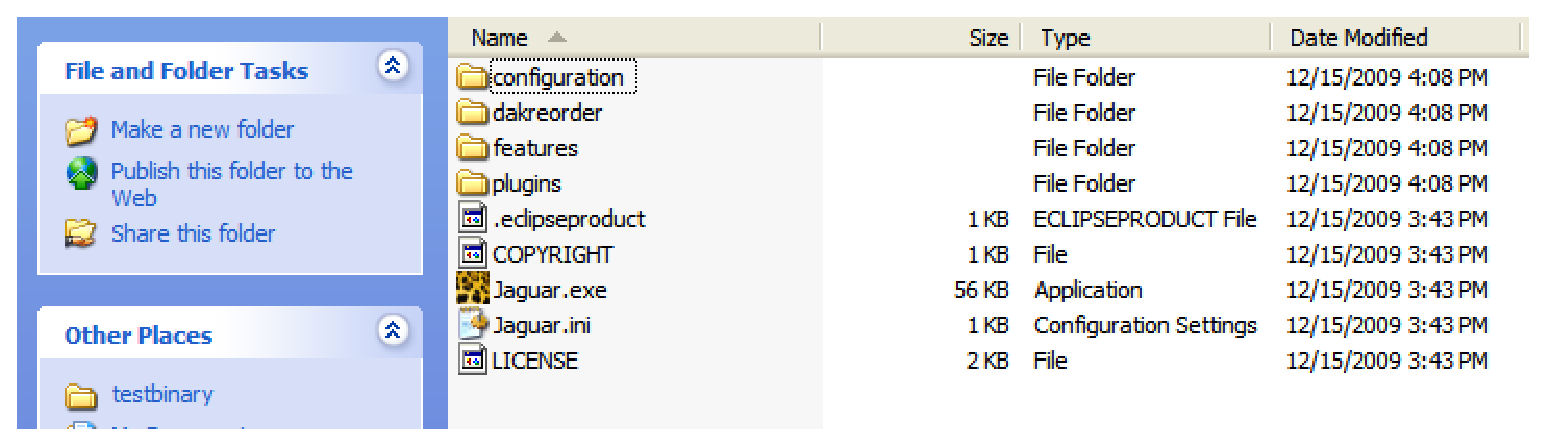
\includegraphics[scale=0.6]{images/jag_package}
  \caption{The JAGUAR installation package.}
  \label{fig:input:jag_package}
\end{figure}

\end{itemize}


\subsection{Running JAGUAR for the First Time}

When starting JAGUAR for the first time, you should see a ``Welcome''
screen.  As can be seen in Figure~\ref{fig:input:jag_welcome}, the
Welcome screen provides quick navigation to many JAGUAR features.
This screen can be closed at anytime by clicking on the ``X'' located
on the Welcome tab and returned to at anytime via the JAGUAR help menu
({\bf Help $\rightarrow$ Welcome}).
\begin{figure}
  \centering
  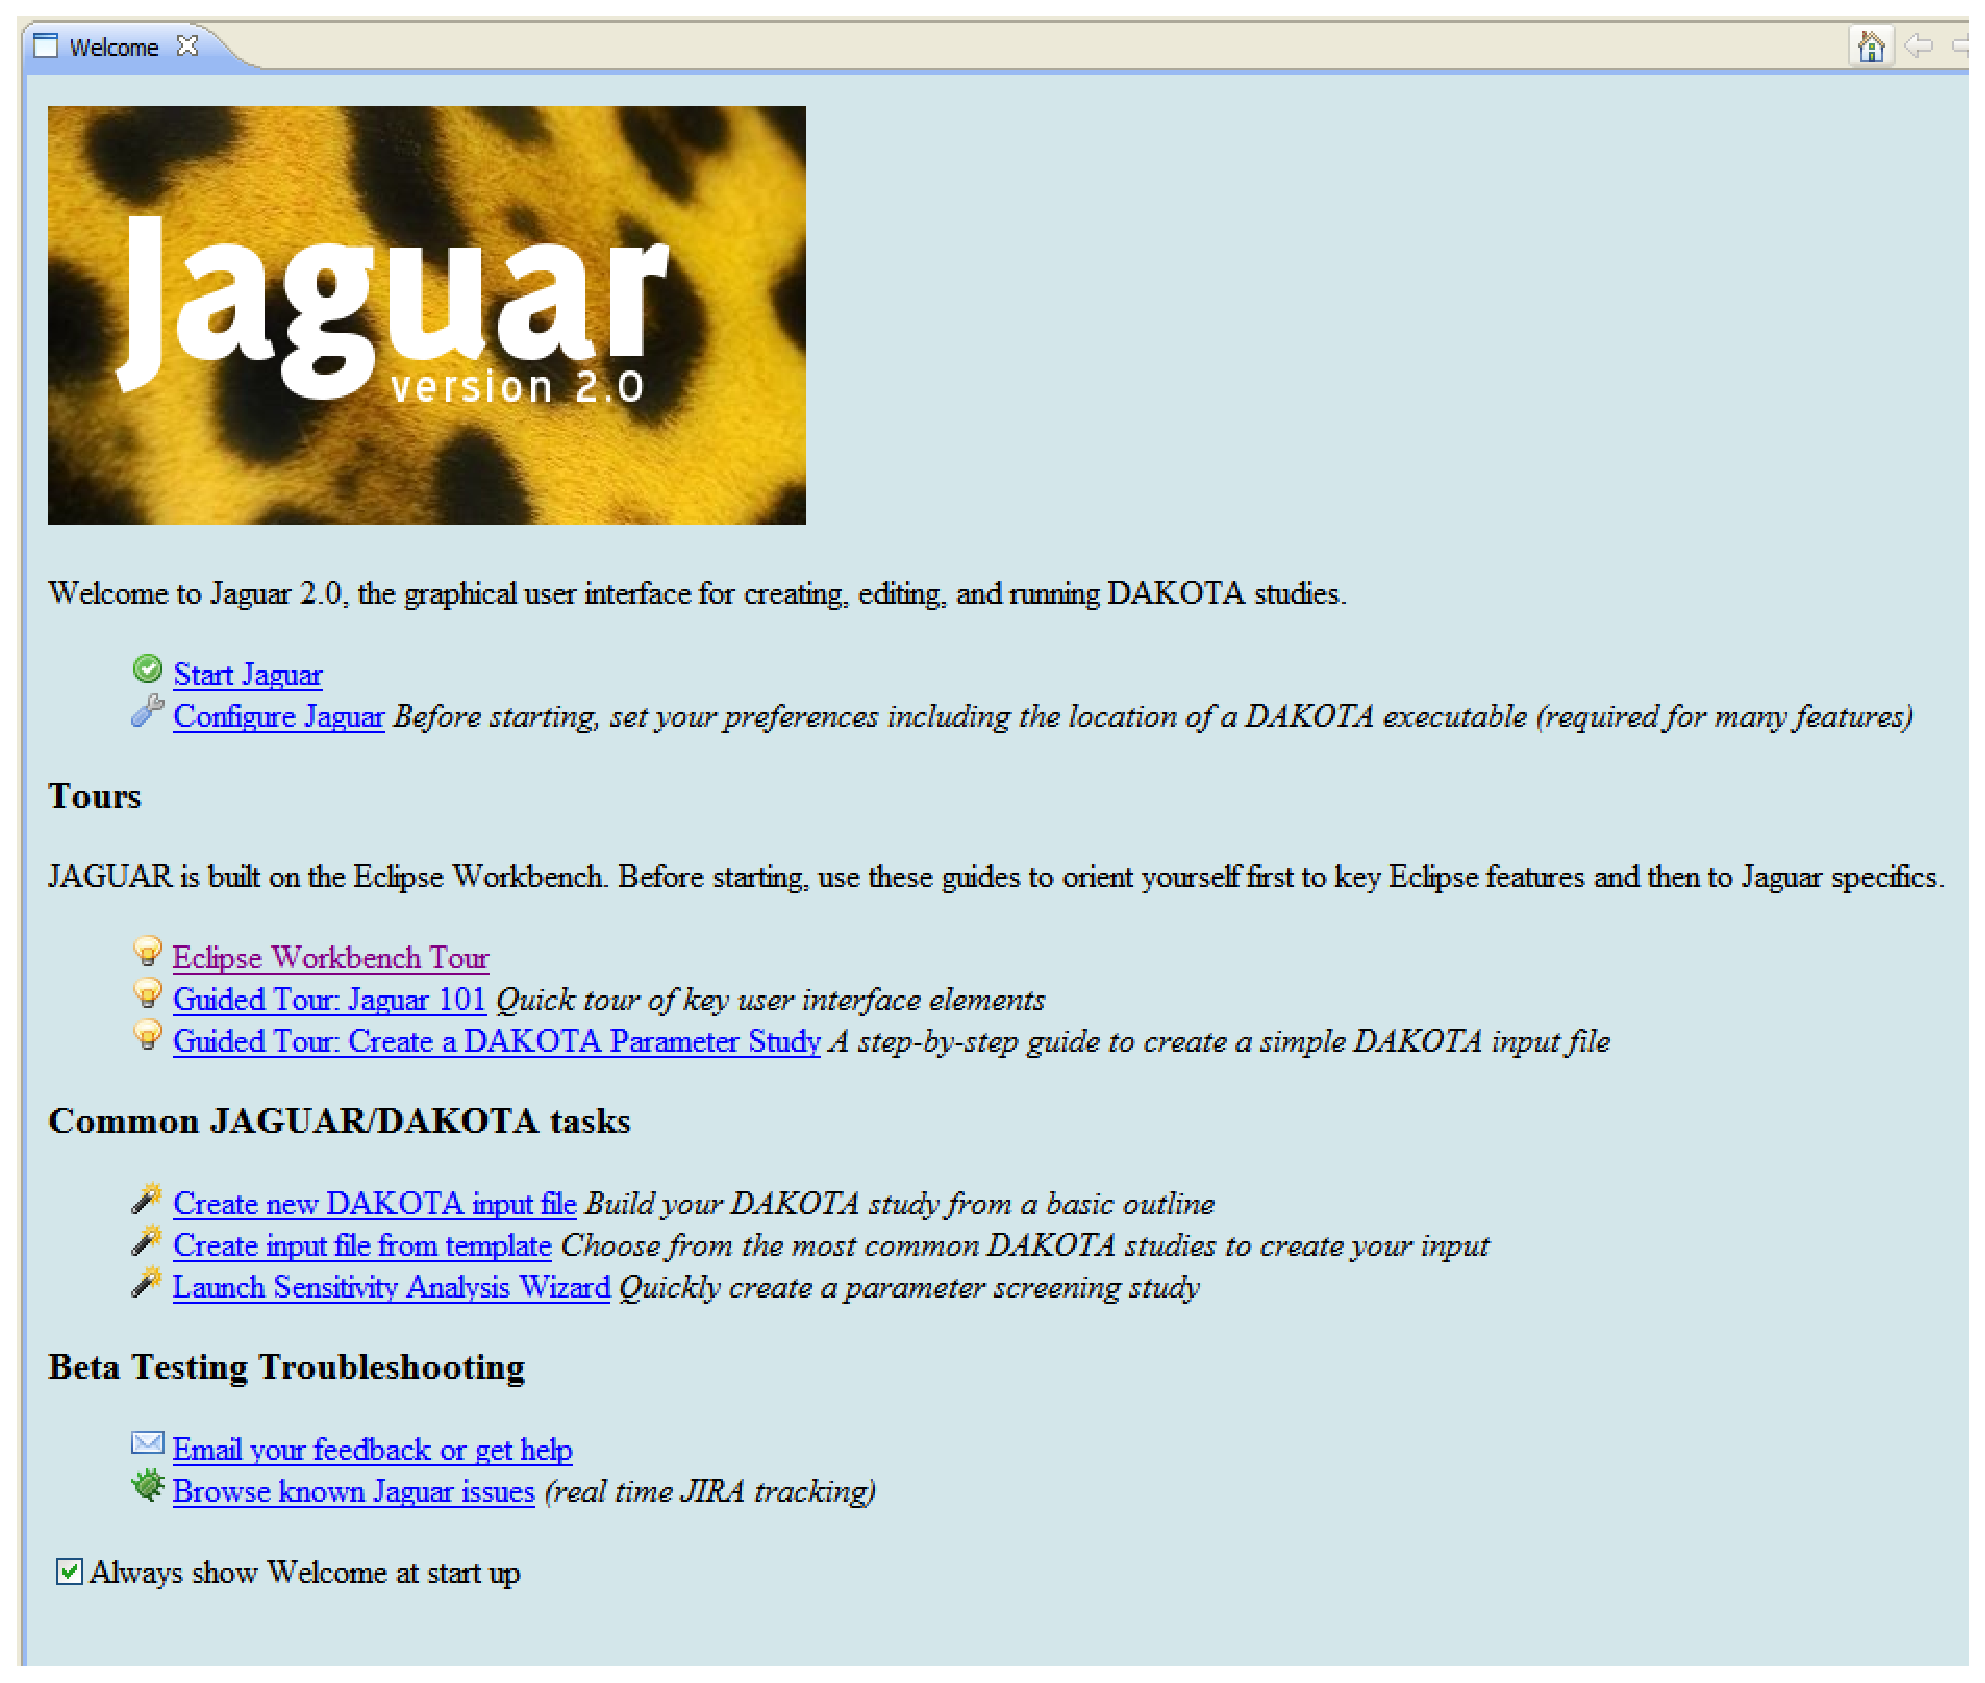
\includegraphics[scale=0.4]{images/jag_welcome}
  \caption{The JAGUAR ``Welcome'' screen.}
  \label{fig:input:jag_welcome}
\end{figure}

\begin{itemize}
\item {\bf Start Jaguar.}  The ``Start Jaguar'' link allows users to
  directly proceed to an empty JAGUAR interface.  

\item {\bf Tours.} The Tours section offers guides for beginning
users.  As JAGUAR is built on the Eclipse Workbench, new users will
benefit from the Eclipse Workbench Tour, a quick online reference for
Eclipse framework features like Views, Perspectives, etc.  The next
two links provides access to guided tours via JAGUAR Cheat Sheets
which are shown in Figure~\ref{fig:input:jag_cheatsheets}.
\begin{figure}
  \centering
  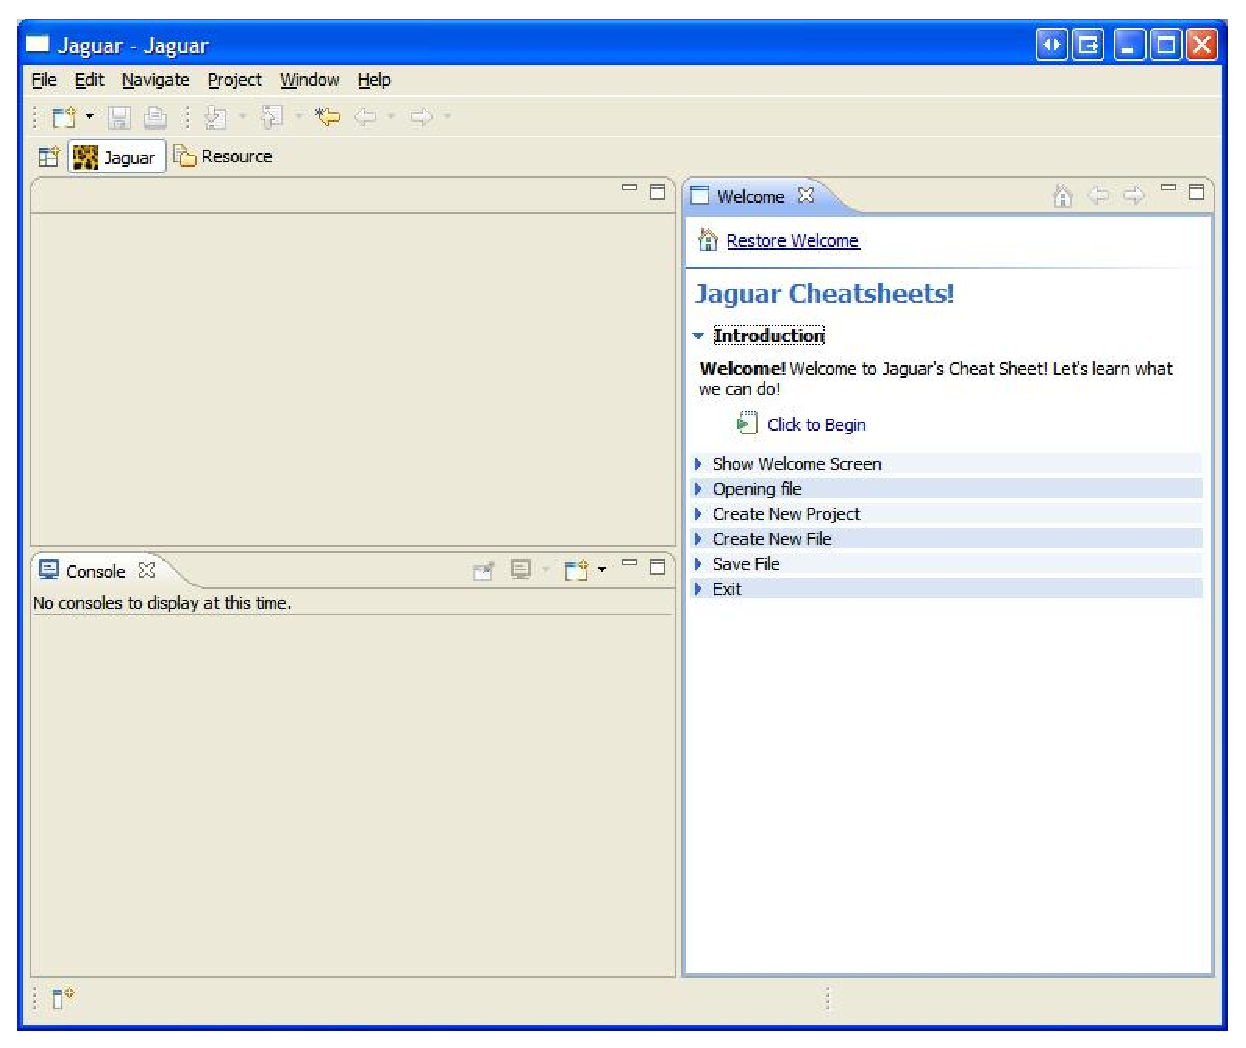
\includegraphics[scale=0.6]{images/jag_cheatsheets}
  \caption{A sample JAGUAR cheatsheet.}
  \label{fig:input:jag_cheatsheets}
\end{figure}
JAGUAR Cheat Sheets are a useful mechanism for quickly learning how to
perform important JAGUAR operations such as opening and saving files.
They utilize an interactive step-by-step approach to guide new users
through JAGUAR.  The Welcome screen is also accessible from Cheat
Sheets.  Cheat Sheets usually dock on the side of the application so
as to not obstruct user interactions, and can always be accessed from
the JAGUAR help menu ({\bf Help $\rightarrow$ Cheat Sheets}).

\item {\bf Create new input file.}  This link creates an empty DAKOTA
  input file.  New input files can also be accessed by selecting {\bf
    New $\rightarrow$ DAKOTA input file} from the File menu.  Users
  must enter a file name for newly-created input files when attempting
  to save them for the first time.

\item {\bf Create new input file from template.}  This links creates a
  new input file from existing DAKOTA templates.  Users must also
  enter a file name when saving these newly-created input files.  This
  action can also be accessed from the File menu by selecting {\bf New
  $\rightarrow$ DAKOTA input file from template}.

\end{itemize}

The remaining two links are used for sending an email to the JAGUAR
developers, and viewing existing JAGUAR bugs.


\subsection{Text Editors}

Figure \ref{fig:input:jag_texteditor} shows an example DAKOTA input
file in the JAGUAR text editor.  The text editor interface is the
first of two primary interfaces that JAGUAR contains for creating and
modifying DAKOTA input files.  For text-based editing, the ``Source''
tab toward the bottom of the JAGUAR window reveals the raw DAKOTA
input file text (likely only comfortable for experienced DAKOTA
users).
\begin{figure}
  \centering
  \includegraphics[scale=0.4]{images/jag_texteditor}
  \caption{The JAGUAR text editor.}
  \label{fig:input:jag_texteditor}
\end{figure}

This text editor supports simple syntax highlighting.  Additional text
editor features planned include syntax completion and
context-sensitive, on-demand tooltip help.


\subsection{Graphical Editors}

JAGUAR's graphical editors are the second primary interface for
creating and modifying DAKOTA input files.  A unique feature of JAGUAR
is that the graphical user interface of these editors is {\em
dynamically} generated from the NIDR input specification for DAKOTA.
When your locally installed version of DAKOTA is updated, you can
point JAGUAR to the new version and it will re-render to match.

Graphical-based editing is conveniently separated into ``Define
Problem'' and ``Define Flow/Iteration'' sections; see the appropriate
tabs toward the bottom of the JAGUAR window in Figure
\ref{fig:input:jag_graphical1}.  ``Define Problem'' is where the
problem to iterate on is defined in terms of models, which map
variables through interfaces to responses.  ``Define Flow/Iteration''
is where a method or methods and possibly a strategy are specified.
\begin{figure}
  \centering
  \includegraphics[scale=0.4]{images/jag_graphical1}
  \caption{The ``Define Problem'' portion of the JAGUAR graphical
    editor.}
  \label{fig:input:jag_graphical1}
\end{figure}

Each pane in the graphical view has two components.  On the left is
the tree hierarchy, which provides users with easy navigation across
the structured input file.  The right side of the view is where
content is displayed and selections may be made.  As an example, see
Figure \ref{fig:input:jag_graphical2}.
\begin{figure}
  \centering
  \includegraphics[scale=0.4]{images/jag_graphical2}
  \caption{Content selected from the left tree hierarchy is displayed
    on the right side of the view.}
  \label{fig:input:jag_graphical2}
\end{figure}

When a top-level element (i.e., Model, Variable Interface, Responses,
Strategy, or Method), represented by a multi-colored brick, is
selected by a user, the right pane will display a top-level overview
of the selection.  From this page, certain top-level elements will
show instance restrictions for a valid input file, allow the user to
create a new instance, and to go directly to or delete an existing
instance.

Within each top-level instance lie unique instances (represented by a
gray brick).  Each instance contains many possible configurable
settings, which are all organized according to their hierarchy as
shown in Figure \ref{fig:input:jag_graphical3}.  We call these
``elements.''
\begin{figure}
  \centering
  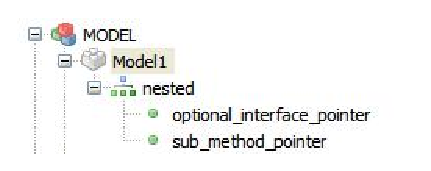
\includegraphics[scale=0.8]{images/jag_graphical3}
  \caption{An organized hierarchy of possible configurable settings.}
  \label{fig:input:jag_graphical3}
\end{figure}

When an instance is selected, its elements are displayed in the right
content pane. (See Figure \ref{fig:input:jag_graphical4}.)  Note that
certain elements have nested elements, which are not immediately
displayed in the content pane.  To view these child elements, select
the element in the left hierarchy tree.
\begin{figure}
  \centering
  \includegraphics[scale=0.4]{images/jag_graphical4}
  \caption{Display of elements from a selected instance.}
  \label{fig:input:jag_graphical4}
\end{figure}

There are five basic types of elements in JAGUAR.
\begin{enumerate}
\item The first is an element without a value.  In Figure
  \ref{fig:input:jag_graphical5}, notice the checkbox to the left of
  the element; this allows the user to enable and disable the element.
  Only enabled elements are represented in the input file, which of
  course can be viewed in the ``Source'' representation (i.e., the
  JAGUAR text editors).  Note that some elements are required, and
  thus cannot be disabled.
\begin{figure}
  \centering
  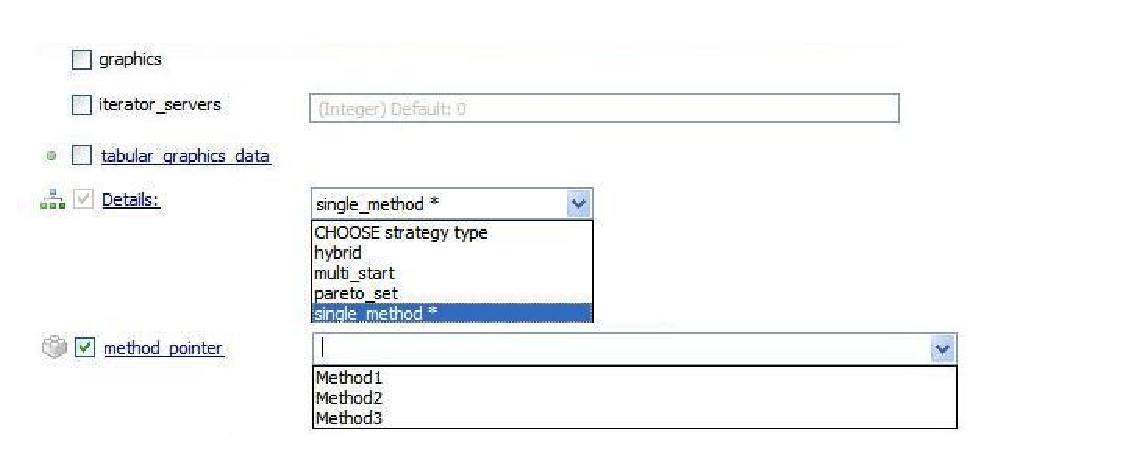
\includegraphics[scale=0.8]{images/jag_graphical5}
  \caption{Different element types in JAGUAR.}
  \label{fig:input:jag_graphical5}
\end{figure}

\item The second element type allows users to set values of type
  Integer, Real, String, or a space-delimited list.

\item Nested elements are supported in JAGUAR, and are indicated by a
  green bullet and the presence of a hyperlink.  Selecting a hyperlink
  is one way to view the nested element in the right-side content
  pane.  The up arrow allows quick return to a parent element in the
  problem specification.

\item Drop-down lists in JAGUAR are indicated by a choice icon.  When
  the list is selected, it behaves like one of the former three
  element types.  In terms of drop-down lists' contents, note that the
  first element functions as a header text whose purpose is to aid the
  user's selection of an appropriate element below.  Asterisks are
  also used to indicate the default element of the list.

\item The fifth and final element is a pointer element that allows the
  reference of other existing elements.  Hyperlinks allow users to
  quickly view that instance in the content pane.  In addition, when
  an unrecognized instance name is manually entered in a pointer
  element, JAGUAR automatically creates that new instance.

\end{enumerate}

Push-up elements allow sub-specifications to be displayed in the
current pane instead of requiring a dive in the tree to see them.
Figures~\ref{fig:input:jaguar_pushup_on}
and~\ref{fig:input:jaguar_pushup_off} show JAGUAR with push-up
elements on (default) and off, respectively.  Control behavior of
push-ups with the upward facing arrow on the top right of the editor
or in preferences.

\begin{figure}
  \centering
  \includegraphics[scale=0.4]{images/jaguar_pushup_on}
  \caption{JAGUAR with push-up elements enabled (default).}
  \label{fig:input:jaguar_pushup_on}
\end{figure}

\begin{figure}
  \centering
  \includegraphics[scale=0.4]{images/jaguar_pushup_off}
  \caption{JAGUAR with push-up elements disabled.}
  \label{fig:input:jaguar_pushup_off}
\end{figure}

The JAGUAR toolbar, shown in Figure~\ref{fig:input:jaguar_toolbar}
offers (from left to right) quick access for running DAKOTA input
files, displaying pretty names instead of keywords, toggling help
text, displaying comments, and toggling push-up elements.

\begin{figure}
  \centering
  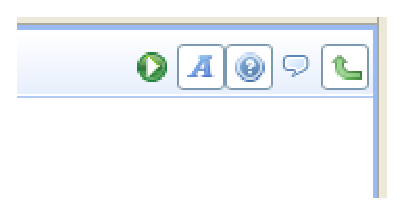
\includegraphics[scale=0.4]{images/jaguar_toolbar}
  \caption{JAGUAR toolbar for running DAKOTA or toggling many
  options.}
  \label{fig:input:jaguar_toolbar}
\end{figure}


\subsection{DAKOTA Execution}

The ``Execute Problem'' tab contains several options for executing
DAKOTA on the active input file, as shown in
Figure~\ref{fig:input:jag_execute}.
\begin{figure}
  \centering
  \includegraphics[scale=0.4]{images/jag_execute}
  \caption{The JAGUAR ``Execute Problem'' tab.}
  \label{fig:input:jag_execute}
\end{figure}
The execute options all rely on a locally installed copy of DAKOTA,
the path to which can be set via Window \textgreater Preferences
\textgreater Jaguar.

Currently four modes of DAKOTA execution are supported:
\begin{itemize}

\item {\bf Check:} While JAGUAR includes considerable input
validation, additional validation is managed solely by DAKOTA's input
parser.  To use DAKOTA to validate the active input file (via {\tt
dakota -check}), click the Check button and view the console output on
the Visualize tab.  You should see a message indicating that the check
completed and should see no errors:

\begin{small}
\begin{verbatim}
Input check completed: problem specification parsed and objects instantiated.
\end{verbatim}
\end{small}

\item {\bf Run:} The run feature supports running DAKOTA on the local
machine using the active input file.  Clicking Run will start DAKOTA
in the same directory as the input file, so any necessary driver
scripts or data files must be present.  View the output from DAKOTA in
the console window:

\begin{verbatim}
<<<<< Iterator multidim_parameter_study completed.
<<<<< Function evaluation summary: 25 total (25 new, 0 duplicate)
<<<<< Best data metrics not defined for generic response functions
<<<<< Single Method Strategy completed.
\end{verbatim}

\item {\bf Pre Run:} Pre-run is a component of the normal DAKOTA run
process.  For select analyzer methods only, e.g., parameter studies
and sampling methods, DAKOTA supports a pre-run mode ({\tt dakota
-pre\_run}), which will generate the set of points at which DAKOTA
will evaluate the model and optionally write them to a tabular file.
The optional checkbox permits saving this generated file.  A
successful pre-run will terminate with a message:

\begin{small}
\begin{verbatim}
Pre-run phase complete: variables written to tabular file my_vars.dat
\end{verbatim}
\end{small}

\item {\bf Post Run:} Post-process user-supplied variables and
function evaluation data, for example, to compute final statistics in
a screening study (the analysis counterpart complementing Pre Run).
Pre-run and post-run are central to the sensitivity analysis wizard.

\end{itemize}

Results from any execute option are displayed on the ``Visualize
Results'' tab as shown in Figure~\ref{fig:input:jaguar_visualize}.

\begin{figure}
  \centering
  \includegraphics[scale=0.4]{images/jaguar_visualize}
  \caption{JAGUAR Visualize Results tab.}
  \label{fig:input:jaguar_visualize}
\end{figure}

Two additional modes will be supported in future JAGUAR versions:
\begin{itemize} 
\item {\bf Core Run:} Perform only the model evaluation (invoke {\tt
analysis\_drivers}) to map variables to responses.  ({\tt dakota
-run})

\item {\bf Remote job submission:} Submit DAKOTA job on a remote
compute cluster and monitor job status.
\end{itemize}


\subsection{Sensitivity Analysis Wizard}

JAGUAR will ultimately provide wizards for creating customized DAKOTA
input files for a variety of common tasks such as optimization,
parameter estimation, and uncertainty quantification.  Presently, one
such wizard exists for creating a Latin hypercube sampling sensitivity
analysis (screening) study, and is accessible from the Welcome screen
and the main File menu ({\bf New $\rightarrow$ Sensitivity Analysis
Wizard}).

Upon launching, select either the variables definition (pre-run) phase
or analysis (post-run) phase (Figure~\ref{fig:input:jaguar_sa_wizard})
\begin{figure}
  \centering
  \includegraphics[scale=0.5]{images/jaguar_sa_wizard}
  \caption{The splash page for the JAGUAR Sensitivity Analysis
  Wizard.}
  \label{fig:input:jaguar_sa_wizard}
\end{figure}

Figure~\ref{fig:input:jag_wizard3} shows the second page of the
sensitivity analysis wizard.  The number of samples, uncertain
(uniformly-distributed) variables, and responses must be specified.
For each specified variable, lower and upper bounds are required;
there are also optional fields for specifying descriptors for each
variable.  After these fields have been complete, the user can
generate the LHS samples in the form of a run matrix using the
``Generate samples'' option, and/or save the input file for the LHS
study using the ``Save input file'' option and specifying a location
for the input file. (Selecting ``Save input file'' will end the
wizard.)
\begin{figure}
  \centering
  \includegraphics[scale=0.5]{images/jag_wizard3}
  \caption{The second page of the JAGUAR Sensitivity Analysis Wizard,
  pre-run phase.}
  \label{fig:input:jag_wizard3}
\end{figure}

Figure~\ref{fig:input:jag_wizard4} shows an example of the final page
of the wizard containing the generated run matrix if the ``Generate
samples'' option is selected.  Note that this option actually executes
the locally-installed version of DAKOTA (in ``pre-run'' mode) to
generate the run matrix.  The page also provides options for saving
both the input file and the generated run matrix.
\begin{figure}
  \centering
  \includegraphics[scale=0.5]{images/jag_wizard4}
  \caption{The final page of the Sensitivity Analysis Wizard, pre-run
  phase.}
  \label{fig:input:jag_wizard4}
\end{figure}

After creating a samples file (run matrix), a use may either add
columns for response data to the file, or run DAKOTA to perform
variable to response mappings, then return to the wizard's post-run
mode.  Figure~\ref{fig:input:jaguar_sa_post_run} shows specification
of the saved input deck from pre-run and the location of the data file
containing the variables and response data to analyze.
\begin{figure}
  \centering
  \includegraphics[scale=0.5]{images/jaguar_sa_post_run}
  \caption{The second page of the JAGUAR Sensitivity Analysis Wizard,
  post-run phase.}
  \label{fig:input:jaguar_sa_post_run}
\end{figure}

\subsection{Generating Input Files from Templates}

There exist many example input files for DAKOTA analysis and studies
that users can build on, customizing their own studies from these
templates.  JAGUAR provides easy access to these templates by allowing
users to generate new input files from a library of templates.  These
templates can be accessed from the Welcome screen, or from the main
File menu ({\bf New $\rightarrow$ DAKOTA input file from template}).

As shown in Figure~\ref{fig:input:jag_template1}, JAGUAR contains a
large library of pre-made input file templates that users can select
from.  After selecting a template upon which to base a new input file,
specify a location to save the new input file (see
Figure~\ref{fig:input:jag_template2}).
\begin{figure}
  \centering
  \includegraphics[scale=0.6]{images/jag_template1}
  \caption{A list of DAKOTA input file templates in JAGUAR}
  \label{fig:input:jag_template1}
\end{figure}
\begin{figure}
  \centering
  \includegraphics[scale=0.6]{images/jag_template2}
  \caption{Specifying a location for saving an input file generated
    from a template.}
  \label{fig:input:jag_template2}
\end{figure}

\newpage
\subsection{Brief tutorial on how to use Jaguar}

Here we provide a simple example originating from the legacy input file dakota\_rosebrock\_2d.in that can be found in the examples/tutorial
directory of the Dakota distributions. To familiarize with Jaguar's basics please follow the steps described below.

Start Jaguar

In the Welcome screen, select ``Configure Jaguar'' or select Window $\Rightarrow$ Preferences (see Figure~\ref{fig:input:0Preferences}).
\begin{itemize}
\item Under Jaguar options, provide your paths for ``DAKOTA executable'', ``Save path'' and ``Templates path''.
\item Select ``OK''.
\end{itemize}
\begin{figure}[htbp]
  \centering
  \includegraphics[scale=0.6]{images/0Preferences}
  \caption{Jaguar Preferences}
  \label{fig:input:0Preferences}
\end{figure}

File $\Rightarrow$ New $\Rightarrow$ DAKOTA input file from template
\begin{itemize}
\item Do either of the following:
\begin{enumerate}
\item Type ``tutorial'' in the quick search bar and select ``Tutorial Rosenbrock''
\item Navigate down and select ``Tutorial Rosenbrock''
\end{enumerate}
\item A preview of the template file should be visible, see Figure~\ref{fig:input:1tutorial}.
\item Select ``Next''
\item Specify a filename such as ``rosenbrock.i''
\item Select ``Finish''
\end{itemize}
\begin{figure}[htbp]
  \centering
  \includegraphics[scale=0.6]{images/1tutorial}
  \caption{DAKOTA input file templates}
  \label{fig:input:1tutorial}
\end{figure}


As in Figure~\ref{fig:input:2rosenbrockfile} notice the following:
\begin{itemize}      
\item Errors with \texttt{direct} and \texttt{analysis\_driver}. This is because the two keywords are out of place (often the case with legacy input files). We will fix this issue later.
\item Mouse over and see the tooltip errors.
\item Mouse over other keywords to see additional information.
\item To run the advanced parsing engine and to format the text, press Ctrl-Shift-F or Edit $\Rightarrow$ Format. Observe the updated rosenbrock\_2d template input file in Figure~\ref{fig:input:3fixed}. 
\item You can always Undo (Ctrl-Z or Edit $\Rightarrow$ ''Undo Typing'') and Redo (Ctrl-Y or Edit $\Rightarrow$ ''Redo Typing'') to compare.
\end{itemize}
\begin{figure}[htbp]
  \centering
  \includegraphics[scale=0.6]{images/2rosenbrockfile}
  \caption{rosenbrock\_2d legacy input file}
  \label{fig:input:2rosenbrockfile}
\end{figure}

In Figure~\ref{fig:input:3fixed} notice the following:
\begin{itemize}
\item cleaner look (unnecessary spaces and newlines removed)
\item \texttt{analysis\_driver} replaced with \texttt{analysis\_drivers} (legacy correction)
\item \texttt{direct} now a sub-element of \texttt{analysis\_drivers} (legacy correction)
\item double quoted ``x2'' replaced with single quoted 'x2' (uniform)
\end{itemize}
\begin{figure}[htbp]
  \centering
  \includegraphics[scale=0.6]{images/3fixed}
  \caption{``Fixed'' rosenbrock\_2d template input file after using the advanced parsing engine}
  \label{fig:input:3fixed}
\end{figure}      

 
To execute click the tab ``(3) Execute Problem'' at the bottom, as in Figure~\ref{fig:input:4ExecuteProblem}. 
\begin{itemize}
\item Click ``Check'' at the top of the page
\end{itemize}
\begin{figure}[htbp]
  \centering
  \includegraphics[scale=0.6]{images/4ExecuteProblem}
  \caption{``Execute Problem'' tab}
  \label{fig:input:4ExecuteProblem}
\end{figure}


In Figure~\ref{fig:input:5Visualize} notice:
\begin{itemize}
\item Actual DAKOTA command (in green) just ran.
\item Output of DAKOTA's check run below.
\end{itemize}
\begin{figure}[htbp]
  \centering
  \includegraphics[scale=0.6]{images/5Visualize}
  \caption{``Visualize Results'' tab}
  \label{fig:input:5Visualize}
\end{figure}


Now go back to the Source (1st tab):
\begin{itemize}
\item Find tabular\_graphics\_data (around line 5), create a new line below and press Ctrl-Space. Notice a list of keywords are listed in a dropdown, see Figure~\ref{fig:input:6Autocomplete}.
\item Press up or down arrows to navigate.
\item Navigate to ``output\_precision'' but DO NOT press Enter.
\begin{figure}[htbp]
  \centering
  \includegraphics[scale=0.6]{images/6Autocomplete}
  \caption{}
  \label{fig:input:6Autocomplete}
\end{figure}
\begin{itemize}
\item Notice that strategy is highlighted in the text, and also listed next to output\_precision. Auto-completing keywords are sorted backwards, meaning they keywords at the top are the closest matching keywords. This helps you discover relevant keywords.
\end{itemize}
\item Select output\_precision
\item Notice auto-complete types in an equal ``='' for you to remind you to enter a value.
\item Type in ``notinteger''.
\item Notice red underline shows an error has occurred.
\item Mouse over it (see Figure~\ref{fig:input:7texterror}).
\begin{figure}[htbp]
  \centering
  \includegraphics[scale=0.6]{images/7texterror}
  \caption{Text error detailed message}
  \label{fig:input:7texterror}
\end{figure}
\item Correct by replacing it with a valid integer
\item On the next line, type in ``iterato''.
\item Right after the ``o'' in ``iterato'', press Ctrl-Space.
\item Notice auto-completion can also finish off half completed keywords. Pick one (see Figure~\ref{fig:input:8iterato}).
\end{itemize}
\begin{figure}[htbp]
  \centering
  \includegraphics[scale=0.6]{images/8iterato}
  \caption{Auto-completion window}
  \label{fig:input:8iterato}
\end{figure}


Save this corrected rosenbrock file as your own template (Figure~\ref{fig:input:9SaveAsTemplate}):
\begin{itemize}
\item File $\Rightarrow$ Save As Template
\item Notice: this path is specified in the Jaguar Preferences you had set earlier.
\item Name it ``Rosenbrock Fixed''
\item Click ``Save''
\end{itemize} 
\begin{figure}[htbp]
  \centering
  \includegraphics[scale=0.6]{images/9SaveAsTemplate}
  \caption{Save As DAKOTA Template Window}
  \label{fig:input:9SaveAsTemplate}
\end{figure}


Close all files (Ctrl-Shift-W) or File $\Rightarrow$ ''Close All''. No need to save changes.


Click on File $\Rightarrow$ New $\Rightarrow$ DAKOTA input file from template 
\begin{itemize}
\item Do either of the following:
\begin{enumerate}
\item Type ``Fixed'' in the quick search bar and select ``Rosenbrock Fixed''
\item Navigate down and select ``Rosenbrock Fixed''
\end{enumerate}
\begin{figure}[htbp]
  \centering
  \includegraphics[scale=0.6]{images/10Template_Rosenbrock}
  \caption{Rosenbrock Fixed DAKOTA Template}
  \label{fig:input:10Template_Rosenbrock}
\end{figure}

\item Notice (see Figure~\ref{fig:input:10Template_Rosenbrock}) that:
\begin{enumerate}
\item This time we are creating an input file from a user-created template.
\item User-created templates do not have stars on them and are listed at the top.
\end{enumerate} 
\item A preview of the template file should be visible.
\item Select ``Next''
\item Specify a filename such as ``rosenbrock\_fixed.i'' 
\item Select ``Finish''
\end{itemize}


This completes the basic tutorial of Jaguar 2.1.

\subsection{Troubleshooting}

In case of errors, please try these options:
\begin{enumerate}
\item  Check if your Java version is supported: ``java-version''. You should have at least Java 1.5
\item  If it is a corrupted workspace, remove the workspace (<User\_folder>/Jaguar\_workspace)
\item  Enable Error Log: Window $\Rightarrow$ Show View $\Rightarrow$ Error Log (see Figure~\ref{fig:input:11ShowView}).
\end{enumerate}

\begin{figure}[htbp]
  \centering
  \includegraphics[scale=0.6]{images/11ShowView}
  \caption{Enabling Jaguar Error Log}
  \label{fig:input:11ShowView}
\end{figure}


Send any errors listed to our support email (jaguar-help@sandia.gov).

\newpage
\section{Data Imports}\label{input:import}

The DAKOTA input file and/or command line may identify additional
files used to import data into DAKOTA.

\subsection{AMPL algebraic mappings: stub.nl, stub.row, and stub.col}

As described in Section~\ref{interfaces:algebraic}, an AMPL
specification of algebraic input-to-output relationships may be
imported into DAKOTA and used to define or augment the mappings of a
particular interface.

\subsection{Genetic algorithm population import}

Genetic algorithms (GAs) from the JEGA and COLINY packages support a 
population import feature using the keywords 
\texttt{initialization\_type flat\_file = \emph{STRING}}.  This is 
useful for warm starting GAs from available data or previous runs.
Refer to the Method Specification chapter in the DAKOTA Reference
Manual~\cite{RefMan} for additional information on this specification.

\subsection{Least squares data import}

Least squares methods can read files of whitespace-separated
experimental data to difference with model results, with one
experimental data point given per model response returned to DAKOTA.
See~\ref{nls:examples} and the DAKOTA Reference Manual for further
details.

\subsection{PCE coefficient import}

Polynomial chaos expansion (PCE) methods compute coefficients for
response expansions which employ a basis of multivariate orthogonal
polynomials.  Normally, the \texttt{polynomial\_chaos} method
calculates these coefficients based either on a spectral projection or
a linear regression (see Section~\ref{uq:expansion}).  However,
DAKOTA also supports the option of importing a set of response PCE
coefficients based on the specification
\texttt{expansion\_import\_file = \emph{STRING}}.  This is useful for
evaluating moments analytically or computing probabilities numerically
from a known response expansion.  Refer to the Method Specification
chapter in the DAKOTA Reference Manual~\cite{RefMan} for additional
information on this specification.

\subsection{Surrogate construction from data files}

Global data fit surrogates may be constructed from a variety of
data sources.  One of these sources is an auxiliary data file,
as specified by the keywords 
\texttt{reuse\_samples samples\_file = \emph{STRING}}.  Refer to the 
Model Specification chapter in the DAKOTA Reference 
Manual~\cite{RefMan} for additional information on this specification.

\subsection{Variables/responses import to post-run}

The post-run mode (supported only for sampling, parameter study, and
DACE methods) requires specification of a file containing parameter
and response data in columnar format.  Columns for variables are
followed by those for responses, with an ignored header row of labels
and then one row per evaluation.  Typically this file would be
generated by executing \texttt{dakota -i dakota.in -pre\_run
::variables.dat} and then adding columns of response data to
variables.dat to make varsresponses.dat.  The file is specified as
follows at the command line:
\begin{small}
\begin{verbatim}
    dakota -i dakota.in -post_run varsresponses.dat::
\end{verbatim}
\end{small}

%PCE coefficients

\chapter{Output from Dakota}\label{output}

\section{Overview of Output Formats}\label{output:overview}

While Dakota primarily targets complex numerical simulation codes run
on massively parallel supercomputers, Dakota's output aims to provide
a succinct, text-based reporting of the progress of the iterations and
function evaluations performed by an algorithm. In addition, Dakota
provides a tabular output format that is useful for data visualization
with external tools and a basic graphical output capability that is
useful as a monitoring tool. The JAGUAR Dakota GUI is an emerging
capability that will provide more advanced visualization facilities in
time.  Dakota also has a number of export capabilities described in
the latter part of this chapter.

\section{Standard Output}\label{output:standard}

Dakota outputs basic information to standard out (screen, terminal,
or console) for each function evaluation, consisting of an evaluation
number, parameter values, execution syntax, the active set vector, and
the response data set. To describe the standard output of Dakota,
optimization of the ``container'' problem (see
Chapter~\ref{additional} for problem formulation) is used as an
example. The input file for this example is shown in
Figure~\ref{output:incont}. In this example, there is one equality
constraint, and Dakota's finite difference algorithm is used to
provide central difference numerical gradients to the NPSOL optimizer.
\begin{figure}
  \begin{small}
    \begin{bigbox}
      \verbatimtabinput[8]{container_opt_npsol.in}
    \end{bigbox}
  \end{small}
  \caption{Dakota input file for the ``container'' test problem --
see \texttt{Dakota/examples/users/container\_opt\_npsol.in} }
  \label{output:incont}
\end{figure}

\clearpage

A partial listing of the Dakota output for the container optimization
example follows:
\begin{small}
\begin{verbatim}
Dakota version 5.4+ (stable) released May  2 2014.
Subversion revision 2508 built May  2 2014 15:26:14.
Running MPI Dakota executable in serial mode.
Start time: Fri May  2 15:38:11 2014

----------------------------------------------------------------
Begin DAKOTA input file
/home/briadam/dakota/build/examples/users/container_opt_npsol.in
----------------------------------------------------------------
# Dakota Input File: container_opt_npsol.in
environment
  graphics

<SNIP>

---------------------
End DAKOTA input file
---------------------

Using Dakota input file '/home/briadam/dakota/build/examples/users/container_opt_npsol.in'
Writing new restart file dakota.rst

>>>>> Executing environment.

>>>>> Running npsol_sqp iterator.

------------------------------------------
Begin Dakota derivative estimation routine
------------------------------------------

>>>>> Initial map for analytic portion of response:

---------------------
Begin Evaluation    1
---------------------
Parameters for evaluation 1:
                      4.5000000000e+00 H
                      4.5000000000e+00 D

blocking fork: container container.in.1 container.out.1

Active response data for evaluation 1:
Active set vector = { 1 1 }
                      1.0713145108e+02 obj_fn
                      8.0444076396e+00 nln_eq_con_1


>>>>> Dakota finite difference gradient evaluation for x[1] + h:

---------------------
Begin Evaluation    2
---------------------
Parameters for evaluation 2:
                      4.5045000000e+00 H
                      4.5000000000e+00 D

blocking fork: container container.in.2 container.out.2

Active response data for evaluation 2:
Active set vector = { 1 1 }
                      1.0719761302e+02 obj_fn
                      8.1159770472e+00 nln_eq_con_1


>>>>> Dakota finite difference gradient evaluation for x[1] - h:

---------------------
Begin Evaluation    3
---------------------
Parameters for evaluation 3:
                      4.4955000000e+00 H
                      4.5000000000e+00 D

blocking fork: container container.in.3 container.out.3

Active response data for evaluation 3:
Active set vector = { 1 1 }
                      1.0706528914e+02 obj_fn
                      7.9728382320e+00 nln_eq_con_1


>>>>> Dakota finite difference gradient evaluation for x[2] + h:

---------------------
Begin Evaluation    4
---------------------
Parameters for evaluation 4:
                      4.5000000000e+00 H
                      4.5045000000e+00 D

blocking fork: container container.in.4 container.out.4

Active response data for evaluation 4:
Active set vector = { 1 1 }
                      1.0727959301e+02 obj_fn
                      8.1876180243e+00 nln_eq_con_1


>>>>> Dakota finite difference gradient evaluation for x[2] - h:

---------------------
Begin Evaluation    5
---------------------
Parameters for evaluation 5:
                      4.5000000000e+00 H
                      4.4955000000e+00 D

blocking fork: container container.in.5 container.out.5

Active response data for evaluation 5:
Active set vector = { 1 1 }
                      1.0698339109e+02 obj_fn
                      7.9013403937e+00 nln_eq_con_1


>>>>> Total response returned to iterator:

Active set vector = { 3 3 } Deriv vars vector = { 1 2 }
                      1.0713145108e+02 obj_fn
                      8.0444076396e+00 nln_eq_con_1
 [  1.4702653619e+01  3.2911324639e+01 ] obj_fn gradient
 [  1.5904312809e+01  3.1808625618e+01 ] nln_eq_con_1 gradient


<SNIP>


>>>>> Dakota finite difference gradient evaluation for x[2] - h:

---------------------
Begin Evaluation   40
---------------------
Parameters for evaluation 40:
                      4.9873894231e+00 H
                      4.0230575428e+00 D

blocking fork: container container.in.40 container.out.40

Active response data for evaluation 40:
Active set vector = { 1 1 }
                      9.8301287596e+01 obj_fn
                     -1.2698647501e-01 nln_eq_con_1


>>>>> Total response returned to iterator:

Active set vector = { 3 3 } Deriv vars vector = { 1 2 }
                      9.8432498116e+01 obj_fn
                     -9.6918029158e-12 nln_eq_con_1
 [  1.3157517860e+01  3.2590159623e+01 ] obj_fn gradient
 [  1.2737124497e+01  3.1548877601e+01 ] nln_eq_con_1 gradient



NPSOL exits with INFORM code = 0 (see "Interpretation of output" section in NPSOL manual)

NOTE: see Fortran device 9 file (fort.9 or ftn09)
      for complete NPSOL iteration history.
<<<<< Function evaluation summary: 40 total (40 new, 0 duplicate)
<<<<< Best parameters          =
                      4.9873894231e+00 H
                      4.0270846274e+00 D
<<<<< Best objective function  =
                      9.8432498116e+01
<<<<< Best constraint values   =
                     -9.6918029158e-12
<<<<< Best data captured at function evaluation 36


<<<<< Iterator npsol_sqp completed.
<<<<< Environment execution completed.
DAKOTA execution time in seconds:
  Total CPU        =       0.03 [parent =   0.023997, child =   0.006003]
  Total wall clock =   0.090703
Exit graphics window to terminate DAKOTA.
\end{verbatim}
\end{small}

The output begins with information on the Dakota version, compilation
date, and run mode.  It then echos the user input file before
proceeding to execution phase.  The lines following ``\texttt{>>>>>
  Running npsol\_sqp iterator.}''  show Dakota performing function
evaluations 1--5 that have been requested by NPSOL. Evaluations 6
through 39 have been omitted from the listing for brevity.

Immediately following the line ``\texttt{Begin Function Evaluation
  1}'', the initial values of the design variables, the syntax of the
blocking fork function evaluation, and the resulting objective and
constraint function values returned by the simulation are listed.  The
values of the design variables are labeled with the tags \texttt{H}
and \texttt{D}, respectively, according to the descriptors given in
the input file, Figure~\ref{output:incont}.  The values of the
objective function and volume constraint are labeled with the tags
\texttt{obj\_fn} and \texttt{nln\_eq\_con\_1}, respectively. Note that
the initial design parameters are infeasible since the equality
constraint is violated ($\ne 0$). However, by the end of the run, the
optimizer finds a design that is both feasible and optimal for this
example. Between the design variables and response values, the content
of the system call to the simulator is displayed as
``\texttt{(container container.in.1 container.out.1)}'', with
\texttt{container} being the name of the simulator and
\texttt{container.in.1} and \texttt{container.out.1} being the names
of the parameters and results files, respectively.

Just preceding the output of the objective and constraint function
values is the line ``\texttt{Active set vector = \{1 1\}}''. The
active set vector indicates the types of data that are required from
the simulator for the objective and constraint functions, and values
of ``\texttt{1}'' indicate that the simulator must return values for
these functions (gradient and Hessian data are not required). For more
information on the active set vector, see Section~\ref{variables:asv}.

Since finite difference gradients have been specified, Dakota computes
their values by making additional function evaluation requests to the
simulator at perturbed parameter values. Examples of the
gradient-related function evaluations have been included in the sample
output, beginning with the line that reads ``\texttt{>>>>> Dakota
  finite difference evaluation for x[1] + h:}''. The resulting finite
difference gradients are listed after function evaluation 5 beginning
with the line ``\texttt{>>>>> Total response returned to iterator:}''.
Here, another active set vector is displayed in the Dakota output
file. The line ``\texttt{Active set vector = \{ 3 3 \}}'' indicates
that the total response resulting from the finite differencing
contains function values and gradients.

The final lines of the Dakota output, beginning with the line
``\texttt{<<<<< Function evaluation summary:}'', summarize the
results of the optimization study. The best values of the optimization
parameters, objective function, and volume constraint are presented
along with the function evaluation number where they occurred, total
function evaluation counts, and a timing summary. In the end, the
objective function has been minimized and the equality constraint has
been satisfied (driven to zero within the constraint tolerance).

The Dakota results may be intermixed with iteration information from
the NPSOL library. For example lines with the heading ``\texttt{Majr
  Minr Step Fun Merit function Norm gZ Violtn nZ Penalty Conv}'' come
from Fortran write statements within NPSOL. The output is mixed since
both Dakota and NPSOL are writing to the same standard output
stream. The relative locations of these output contributions can vary
depending on the specifics of output buffering and flushing on a
particular platform and depending on whether or not the standard
output is being redirected to a file. In some cases, output from the
optimization library may appear on each iteration (as in this
example), and in other cases, it may appear at the end of the Dakota
output. Finally, a more detailed summary of the NPSOL iterations is
written to the Fortran device 9 file (e.g., \texttt{fort.9} or
\texttt{ftn09}).

\section{Tabular Output Data}\label{output:tabular}

Dakota has the capability to print the iteration history in tabular
form to a file. The keyword\\
\texttt{tabular\_graphics\_data} needs to be included in the
environment specification (see Figure~\ref{output:incont}). The
primary intent of this capability is to facilitate the transfer of
Dakota's iteration history data to an external mathematical analysis
and/or graphics plotting package (e.g., MATLAB, TECplot, Excel,
S-plus, Minitab). Any evaluations from Dakota's internal finite
differencing are suppressed, to facilitate rapid plotting of the most
critical data.  This suppression of lower level data is consistent
with the data that is sent to the graphics windows, as described in
Section~\ref{output:graphics}. If this data suppression is
undesirable, Section~\ref{restart:utility:tabular} describes an
approach where every function evaluation, even the ones from finite
differencing, can be saved to a file in tabular format.

The default file name for the tabular output data is
``\texttt{dakota\_tabular.dat}'' and the output from the ``container''
optimization problem is shown in Figure~\ref{output:tabcont}. This
annotated tabular format (see Section~\ref{input:tabularformat}) file
contains the complete history of data requests from NPSOL (8 requests
map into a total of 40 function evaluations when including the central
finite differencing). The first column is the data request number, the
second and third columns are the design parameter values (labeled in
the example as ``\texttt{H}'' and ``\texttt{D}''), the fourth column
is the objective function (labeled ``\texttt{obj\_fn}''), and the
fifth column is the nonlinear equality constraint (labeled
``\texttt{nln\_eq\_con\_1}'').

\begin{figure}
\begin{bigbox}
\begin{small}
\begin{verbatim}
%eval_id              H              D         obj_fn   nln_eq_con_1 
       1            4.5            4.5    107.1314511     8.04440764 
       2    5.801246882    3.596476363    94.33737399    -4.59103645 
       3    5.197920019    3.923577479     97.7797214  -0.6780884711 
       4    4.932877133    4.044776216    98.28930566  -0.1410680284 
       5    4.989328733    4.026133158     98.4270019 -0.005324671422 
       6    4.987494493    4.027041977    98.43249058 -7.307058453e-06 
       7    4.987391669     4.02708372    98.43249809 -2.032538049e-08 
       8    4.987389423    4.027084627    98.43249812 -9.691802916e-12 
\end{verbatim}
\end{small}
\end{bigbox}
\caption{Dakota's tabular output file showing the iteration history of
the ``container'' optimization problem.} \label{output:tabcont}
\end{figure}

\section{Graphics Output}\label{output:graphics}

Graphics capabilities are available for monitoring the progress of an
iterative study. The graphics option is invoked by adding the
\texttt{graphics} flag in the environment specification of the Dakota
input file (see Figure~\ref{output:incont}). The graphics display
the values of each response function (e.g., objective and constraint
functions) and each parameter for the function evaluations in the
study. As for the tabular output described in
Section~\ref{output:tabular}, internal finite difference evaluations
are suppressed in order to omit this clutter from the graphics.
Figure~\ref{output:2dcont} shows the optimization iteration history
for the container example.

If Dakota is executed on a remote machine, the DISPLAY variable in the
user's UNIX environment~\cite{Gil92} may need to be set to the local
machine in order to display the graphics window. 

\begin{figure}
\centering
\includegraphics[width=\textwidth]{images/container_graphic}
\caption{Dakota 2D graphics for ``container'' problem showing history of
an objective function, an equality constraint, and two variables.}
\label{output:2dcont}
\end{figure}

The scroll bars which are located on each graph below and to the right
of each plot may be operated by dragging on the bars or pressing the
arrows, both of which result in expansion/contraction of the axis
scale. Clicking on the ``Options'' button results in the window shown
in Figure~\ref{output:2dcontoptions}, which allows the user to include
min/max markers on the vertical axis, vertical and horizontal axis
labels, and a plot legend within the corresponding graphics plot.  In
addition, the values of either or both axes may be plotted using a
logarithmic scale (so long as all plot values are greater than zero)
and an encapsulated postscript (EPS) file, named 
\texttt{dakota\_graphic\_\emph{i}.eps} where \emph{i} is the plot 
window number, can be created using the ``Print'' button.
\begin{figure}
\centering
\includegraphics[scale=0.6]{images/container_graphic_options}
\caption{Options for Dakota 2D graphics.}
\label{output:2dcontoptions}
\end{figure}


\section{Error Messages Output}\label{output:error}

A variety of error messages are printed by Dakota in the event that an
error is detected in the input specification. Some of the more common
input errors, and the associated error messages, are described below.
See also the Common Specification Mistakes section in the Dakota
Reference Manual~\cite{RefMan}.

Incorrectly spelled specifications, such as 
\texttt{``numericl\_gradients''}, will result in error messages of the form:
\begin{small}
\begin{verbatim}
Input line 31: unrecognized identifier 'numericl_gradients'.
Input line 31: unrecognized identifier 'method_source'.
Input line 31: unrecognized identifier 'dakota'.
Input line 31: unrecognized identifier 'interval_type'.
Input line 31: unrecognized identifier 'central'.
Input line 31: unrecognized identifier 'fd_gradient_step_size'.
Input line 31: One of the following 4 entities
must be specified for responses...
	analytic_gradients
	mixed_gradients
	no_gradients
	numerical_gradients
\end{verbatim}
\end{small}
In this example the line numbers given are approximate, as all input
following an errant keywords is considered a single line through the
end of the block.

The input parser catches syntax errors, but not logic errors. The fact
that certain input combinations are erroneous must be detected after
parsing, at object construction time. For example, if a
\texttt{no\_gradients} specification for a response data set is
combined with selection of a gradient-based optimization method, then
this error must be detected during set-up of the optimizer (see last
line of listing):
\begin{small}
\begin{verbatim}
Error: gradient-based minimizers require a gradient specification.
\end{verbatim}
\end{small}
Many such errors can be detected earlier by running \texttt{dakota
  -check}.

Another common mistake involves a mismatch between the amount of data
expected on a function evaluation and the data returned by the user's
simulation code or driver. The available response data is specified in
the responses keyword block, and the subset of this data needed for a
particular evaluation is managed by the active set vector. For
example, if Dakota expects function values and gradients to be
returned (as indicated by an active set vector containing 3's), but
the user's simulation code only returns function values, then the
following error message is generated:
\begin{small}
\begin{verbatim}
    At EOF: insufficient data for functionGradient 1
\end{verbatim}
\end{small}

Unfortunately, descriptive error messages are not available for all
possible failure modes of Dakota. If you encounter core dumps,
segmentation faults, or other failures, please request help using the
support mechanisms described on the
\href{http://dakota.sandia.gov/}{Dakota website}.


\section{PCE coefficient export}\label{sec:output:pce}

Polynomial chaos expansion (PCE) methods compute coefficients for
response expansions which employ a basis of multivariate orthogonal
polynomials.  The \texttt{polynomial\_chaos} method calculates these
coefficients based on a number of approaches described in
Section~\ref{uq:expansion}).  One may output the PCE coefficients to a
file using the keyword \texttt{export\_expansion\_file =
  \emph{STRING}}.  Each row of the exported file will contain a
coefficient, followed by the multi-index indicating which basis terms
correspond to it.

\section{Surrogate Model Exports}

A number of Dakota surrogate models, including some stochastic
expansion approaches support the keyword \texttt{export\_points\_file
  = \emph{STRING}}.  When specified, any approximate evaluations
performed on the surrogate model will be output to the specified data
file.  This facilitates plotting or external diagnostics of the
surrogate model.

In addition the Surfpak family of global surrogate models supports
export (serialization) of surrogate models to text ({\tt .sps}) or
binary ({\tt .bsps}) model files.  These files are not human readable
(and don't contain an explicit algebraic form of the response surface
model).  Instead they may be imported into the {\tt surfpack}
executable or library API for evaluation, bypassing the reconstruction
of the surrogate model from build data.

\section{Variables Output from Pre-run}

The pre-run mode (supported only for select methods) permits
specification of an output file to which Dakota will write parameter
(variables) data in annotated format (see
Section~\ref{input:tabularformat}) with data columns corresponding to
each variable.  This file can be generated with sampling, parameter
study, and DACE methods by invoking
\begin{small}
\begin{verbatim}
    dakota -i dakota.in -pre_run ::variables.dat
\end{verbatim}
\end{small}
for example, to output the variables (samples) in an LHS study.

% LocalWords:  NPSOL npsol sqp fn nln eq infeasible differencing Majr Minr gZ
% LocalWords:  Violtn nZ Conv Fortran Fortran ftn09 MATLAB TECplot Minitab dat
% LocalWords:  dakota 2D EPS eps numericl combinations PCE multi Pre pre LHS

\chapter{Advanced Methods}\label{adv_meth}

\section{Overview}\label{adv_meth:overview}

A variety of ``meta-algorithm'' capabilities have been developed in 
order to provide a mechanism for employing individual iterators and 
models as reusable components within higher-level solution approaches. 
%It was driven by the observed need for ``meta-optimization'' and other 
%high level systems analysis procedures in real-world engineering 
%design problems. 
This capability allows the use of existing iterative algorithm and
computational model software components as building blocks to
accomplish more sophisticated studies, such as hybrid,
multistart, Pareto, or surrogate-based minimization.  Further
multi-component capabilities are enabled by the model recursion
capabilities described in Chapter~\ref{models} with specific examples
in Chapter~\ref{adv_models}.
%When these model recursion specifications are sufficient to completely
%describe a multi-iterator, multi-model solution approach, then a
%separate meta-iterator specification is not used (see
%Chapter~\ref{adv_models} for examples).

\section{Hybrid Minimization}\label{adv_meth:hybrid}

In the hybrid minimization method (keyword: \texttt{hybrid}), a
sequence of minimization methods are applied to find an optimal design
point. The goal of this method is to exploit the strengths of
different minimization algorithms through different stages of the
minimization process. Global/local optimization hybrids (e.g., genetic
algorithms combined with nonlinear programming) are a common example
in which the desire for a global optimum is balanced with the need for
efficient navigation to a local optimum. An important related feature
is that the sequence of minimization algorithms can employ models of
varying fidelity. In the global/local case, for example, it would
often be advantageous to use a low-fidelity model in the global search
phase, followed by use of a more refined model in the local search
phase.

The specification for hybrid minimization involves a list of
method identifier strings, and each of the corresponding method
specifications has the responsibility for identifying the model
specification (which may in turn identify variables, interface, and
responses specifications) that each method will use (see the Dakota
Reference Manual~\cite{RefMan} and the example discussed below).
Currently, only the sequential hybrid approach is available. The
\texttt{embedded} and \texttt{collaborative} approaches are
not fully functional at this time.

In the \texttt{sequential} hybrid minimization approach, a sequence
of minimization methods is invoked in the order specified in the
Dakota input file. After each method completes execution, 
the best solution or solutions from that method are used as the
starting point(s) for the following method. 
The number of solutions transferred 
is defined by how many that method can generate and how many the 
user specifies with the individual method keyword \texttt{final\_solutions}. 
For example, currently only a few of the global optimization methods such as 
genetic algorithms (e.g. \texttt{moga} and \texttt{coliny\_ea}) and 
sampling methods return multiple solutions.  In this case, 
the specified number of solutions from the previous 
method will be used to initialize the subsequent method.  If the subsequent 
method cannot accept multiple input points (currently only a few methods 
such as the genetic algorithms in JEGA allow multiple input points), then 
multiple instances of the subsequent method are generated, each one 
initialized by one of the optimal solutions from the previous method. 
For example, if LHS sampling were run as the first method and 
the number of final solutions was 10 and the DOT conjugate gradient 
was the second method, there would be 10 instances of \texttt{dot\_frcg} 
started, each with a separate LHS sample solution as its initial point. 
Method switching is governed
by the separate convergence controls of each method; that is,
\emph{each method is allowed to run to its own internal definition of
completion without interference}. Individual method completion may be
determined by convergence criteria (e.g.,
\texttt{convergence\_tolerance}) or iteration limits (e.g.,
\texttt{max\_iterations}).  

%The \texttt{adaptive} option
%is similar, with the difference that the progress of each method is
%monitored and method switching is enforced according to
%externally-defined relative progress metrics.  

%The \texttt{embedded} approach is restricted to special tightly-coupled
%hybrid algorithms in which local searches are used periodically to
%accelerate a global search.  These hybrids do not contain a discrete
%method switch, but rather repeatedly apply a local algorithm within
%the context of the global algorithm.

Figure~\ref{adv_meth:figure01} shows a Dakota input file that specifies
a sequential hybrid optimization method to solve the
``textbook'' optimization test problem.
The \texttt{textbook\_hybrid\_strat.in} file
provided in {\tt Dakota/examples/users} starts with a
\texttt{coliny\_ea} solution which feeds its best point into a
\texttt{coliny\_pattern\_search} optimization which feeds its best
point into \texttt{optpp\_newton}. While this approach is overkill for
such a simple problem, it is useful for demonstrating the coordination
between multiple sub-methods in the hybrid minimization algorithm.

The three optimization methods are identified using the
\texttt{method\_list} specification in the hybrid method section of the
input file. The identifier strings listed in the specification are
`\texttt{GA}' for genetic algorithm, `\texttt{PS}' for pattern search,
and `\texttt{NLP}' for nonlinear programming. Following the hybrid method
keyword block are the three corresponding method keyword blocks. Note
that each method has a tag following the \texttt{id\_method} keyword
that corresponds to one of the method names listed in the hybrid method
keyword block. By following the identifier tags from \texttt{method}
to \texttt{model} and from \texttt{model} to \texttt{variables},
\texttt{interface}, and \texttt{responses}, it is easy to see the
specification linkages for this problem. The GA optimizer runs first
and uses model `\texttt{M1}' which includes variables `\texttt{V1}',
interface `\texttt{I1}', and responses `\texttt{R1}'. 
Note that in the specification, \texttt{final\_solutions=1}, 
so only one (the best) solution is returned from the GA.  
However, it is possible to change this to \texttt{final\_solutions=5}
and get five solutions passed from the GA to the Pattern Search
(for example).  Once the GA is complete, the PS optimizer starts from the 
best GA result and again
uses model `\texttt{M1}'. Since both GA and PS are nongradient-based
optimization methods, there is no need for gradient or Hessian
information in the `\texttt{R1}' response keyword block. The NLP
optimizer runs last, using the best result from the PS method as its
starting point.  It uses model `\texttt{M2}' which includes the same
`\texttt{V1}' and `\texttt{I1}' keyword blocks, but uses the responses
keyword block `\texttt{R2}' since the full Newton optimizer used in
this example (\texttt{optpp\_newton}) needs analytic gradient and
Hessian data to perform its search.
\begin{figure}
  \centering
  \begin{bigbox}
    \begin{tiny}
      \verbatimtabinput[8]{textbook_hybrid_strat.in}
    \end{tiny}
  \end{bigbox}
  \caption{Dakota input file for a sequential hybrid optimization method --
see \texttt{Dakota/examples/users/textbook\_hybrid\_strat.in} }
  \label{adv_meth:figure01}
\end{figure}

\section{Multistart Local Minimization}\label{adv_meth:multistart}

A simple, heuristic, global minimization technique is to use many
local minimization runs, each of which is started from a different
initial point in the parameter space. This is known as multistart
local minimization. This is an attractive method in situations where
multiple local optima are known or expected to exist in the parameter
space. However, there is no theoretical guarantee that the global
optimum will be found. This approach combines the efficiency of local
minimization methods with a user-specified global stratification
(using a specified \texttt{starting\_points} list, a number of
specified \texttt{random\_starts}, or both; see the Dakota Reference
Manual~\cite{RefMan} for additional specification details). Since
solutions for different starting points are independent, parallel
computing may be used to concurrently run the local minimizations.

An example input file for multistart local optimization on the
``quasi\_sine'' test function (see \texttt{quasi\_sine\_fcn.C} in
\texttt{Dakota\_Source/test}) is shown in Figure~\ref{adv_meth:figure02}. 
The method keyword block in the input file contains the keyword
\texttt{multi\_start}, along with the set of starting points (3 random 
and 5 listed) that will be used for the optimization runs. The other
keyword blocks in the input file are similar to what would be used in
a single optimization run.

\begin{figure}
  \centering
  \begin{bigbox}
    \begin{small}
      \verbatimtabinput[8]{qsf_multistart_strat.in}
    \end{small}
  \end{bigbox}
  \caption{Dakota input file for a multistart local optimization method --
see \texttt{Dakota/examples/users/qsf\_multistart\_strat.in} }
  \label{adv_meth:figure02}
\end{figure}

The \texttt{quasi\_sine} test function has multiple local minima, but
there is an overall trend in the function that tends toward the global
minimum at $(x1,x2)=(0.177,0.177)$. See~\cite{Giu00} for more
information on this test function. Figure~\ref{adv_meth:figure03} shows
the results summary for the eight local optimizations performed. From
the five specified starting points and the 3 random starting points
(as identified by the \texttt{x1}, \texttt{x2} headers), the eight
local optima (as identified by the \texttt{x1*},
\texttt{x2*} headers) are all different and only one of the local
optimizations finds the global minimum.

\begin{figure}
\centering
\begin{bigbox}
\begin{footnotesize}
\begin{verbatim}
<<<<< Results summary:
   set_id             x1             x2            x1*            x2*         obj_fn 
        1           -0.8           -0.8  -0.8543728666  -0.8543728666   0.5584096919 
        2           -0.8            0.8  -0.9998398719    0.177092822    0.291406596 
        3            0.8           -0.8    0.177092822  -0.9998398719    0.291406596 
        4            0.8            0.8   0.1770928217   0.1770928217   0.0602471946 
        5              0              0  0.03572926375  0.03572926375  0.08730499239 
        6  -0.7767971993  0.01810943539  -0.7024118387  0.03572951143   0.3165522387 
        7  -0.3291571008  -0.7697378755   0.3167607374  -0.4009188363   0.2471403213 
        8   0.8704730469   0.7720679005    0.177092899   0.3167611757  0.08256082751 
\end{verbatim}
\end{footnotesize}
\end{bigbox}
\caption{Dakota results summary for a multistart local optimization method.}
\label{adv_meth:figure03}
\end{figure}

\section{Pareto Optimization}\label{adv_meth:pareto}

The Pareto optimization method (keyword: \texttt{pareto\_set}) is
one of three multiobjective optimization capabilities discussed in
Section~\ref{opt:additional:multiobjective}. In the Pareto
optimization method, multiple sets of multiobjective weightings are
evaluated. The user can specify these weighting sets in the method
keyword block using a \texttt{multi\_objective\_weight\_sets} list, a
number of \texttt{random\_weight\_sets}, or both (see the Dakota
Reference Manual~\cite{RefMan} for additional specification details).

Dakota performs one multiobjective optimization problem for each set
of multiobjective weights. The collection of computed optimal
solutions form a Pareto set, which can be useful in making trade-off
decisions in engineering design. Since solutions for different
multiobjective weights are independent, parallel computing may be used
to concurrently execute the multiobjective optimization problems.

Figure~\ref{adv_meth:figure05} shows the results summary for the
Pareto-set optimization method. For the four multiobjective
weighting sets (as identified by the \texttt{w1}, \texttt{w2},
\texttt{w3} headers), the local optima (as identified by the
\texttt{x1}, \texttt{x2} headers) are all different and correspond to
individual objective function values of ($f_1,f_2,f_3$) =
(0.0,0.5,0.5), (13.1,-1.2,8.16), (532.,33.6,-2.9), and (0.125,0.0,0.0)
(note: the composite objective function is tabulated under the
\texttt{obj\_fn} header).  The first three solutions reflect exclusive
optimization of each of the individual objective functions in turn,
whereas the final solution reflects a balanced weighting and the
lowest sum of the three objectives.  Plotting these ($f_1,f_2,f_3$)
triplets on a 3-dimensional plot results in a Pareto surface (not
shown), which is useful for visualizing the trade-offs in the
competing objectives.

\begin{figure}
  \centering
  \begin{bigbox}
    \begin{small}
      \verbatimtabinput[8]{textbook_pareto_strat.in}
    \end{small}
  \end{bigbox}
  \caption{Dakota input file for the Pareto optimization method --
see \texttt{Dakota/examples/users/textbook\_pareto\_strat.in} }
  \label{adv_meth:figure04}
\end{figure}

\begin{figure}
\centering
\begin{bigbox}
\begin{scriptsize}
\begin{verbatim}
<<<<< Results summary:
   set_id             w1             w2             w3             x1             x2         obj_fn
        1              1              0              0   0.9996554048    0.997046351 7.612301561e-11
        2              0              1              0            0.5            2.9           -1.2
        3              0              0              1            5.8 1.12747589e-11           -2.9
        4          0.333          0.333          0.333            0.5   0.5000000041       0.041625
\end{verbatim}
\end{scriptsize}
\end{bigbox}
\caption{Dakota results summary for the Pareto-set optimization
  method.}
\label{adv_meth:figure05}
\end{figure}

\section{Mixed Integer Nonlinear Programming (MINLP)}\label{adv_meth:minlp}

Many nonlinear optimization problems involve a combination of discrete
and continuous variables. These are known as mixed integer nonlinear
programming (MINLP) problems. A typical MINLP optimization problem is
formulated as follows:

\begin{eqnarray}
  \hbox{minimize:} & & f(\mathbf{x,d})\nonumber\\
  \hbox{subject to:} & & \mathbf{g}_{L} \leq \mathbf{g(x,d)}
    \leq \mathbf{g}_{U}\nonumber\\
  & & \mathbf{h(x,d)}=\mathbf{h}_{t}\label{adv_meth:equation01}\\
  & & \mathbf{x}_{L} \leq \mathbf{x} \leq \mathbf{x}_{U}\nonumber\\
  & & \mathbf{d} \in \{-2,-1,0,1,2\}\nonumber
\end{eqnarray}

where $\mathbf{d}$ is a vector whose elements are integer values. In
situations where the discrete variables can be temporarily relaxed
(i.e., noncategorical discrete variables, see
Section~\ref{variables:design:ddv}), the branch-and-bound algorithm
can be applied. Categorical variables (e.g., true/false variables,
feature counts, etc.) that are not relaxable cannot be used with the
branch and bound method.  During the branch and bound process, the
discrete variables are treated as continuous variables and the
integrality conditions on these variables are incrementally enforced
through a sequence of optimization subproblems.  By the end of this
process, an optimal solution that is feasible with respect to the
integrality conditions is computed.

Dakota's branch and bound method (keyword:
\texttt{branch\_and\_bound}) can solve optimization problems having
either discrete or mixed continuous/discrete variables. This method
uses the parallel branch-and-bound algorithm from the PEBBL software
%package~\cite{Eck97,Eck01} to generate a series of optimization
package~\cite{Eck09} to generate a series of optimization
subproblems (``branches''). These subproblems are solved as continuous
variable problems using any of Dakota's nonlinear optimization
algorithms (e.g., DOT, NPSOL). When a solution to a branch is feasible
with respect to the integrality constraints, it provides an upper
bound on the optimal objective function, which can be used to prune
branches with higher objective functions that are not yet
feasible. Since solutions for different branches are independent,
parallel computing may be used to concurrently execute the
optimization subproblems.

PEBBL, by itself, targets the solution of mixed integer linear
programming (MILP) problems, and through coupling with Dakota's
nonlinear optimizers, is extended to solution of MINLP problems. In
the case of MILP problems, the upper bound obtained with a feasible
solution is an exact bound and the branch and bound process is
provably convergent to the global minimum. For nonlinear problems
which may exhibit nonconvexity or multimodality, the process is
heuristic in general, since there may be good solutions that are
missed during the solution of a particular branch. However, the
process still computes a series of locally optimal solutions, and is
therefore a natural extension of the results from local optimization
techniques for continuous domains. Only with rigorous global
optimization of each branch can a global minimum be guaranteed when
performing branch and bound on nonlinear problems of unknown
structure.

In cases where there are only a few discrete variables and when the
discrete values are drawn from a small set, then it may be reasonable
to perform a separate optimization problem for all of the possible
combinations of the discrete variables. However, this brute force
approach becomes computationally intractable if these conditions are
not met. The branch-and-bound algorithm will generally require
solution of fewer subproblems than the brute force method, although it
will still be significantly more expensive than solving a purely
continuous design problem.

\subsection{Example MINLP Problem}\label{adv_meth:minlp:example}

As an example, consider the following MINLP problem~\cite{Eld99}:

\begin{eqnarray}
  \hbox{minimize:} & &
  f(\mathbf{x})=\sum_{i=1}^{6}(x_{i}-1.4)^{4}\nonumber\\
  & & g_{1}=x_{1}^{2}-\frac{x_{2}}{2} \leq 0\nonumber\\
  & & g_{2}=x_{2}^{2}-\frac{x_{1}}{2} \leq 0\label{adv_meth:equation02}\\
  & & -10 \leq x_{1},x_{2},x_{3},x_{4} \leq 10\nonumber\\
  & & x_{5},x_{6} \in \{0,1,2,3,4\}\nonumber
\end{eqnarray}

This problem is a variant of the textbook test problem described in
Section~\ref{additional:textbook}. In addition to the introduction of
two integer variables, a modified value of $1.4$ is used inside the
quartic sum to render the continuous solution a non-integral solution.
%Figure~\ref{adv_meth:figure06} shows a Dakota input file for solving this
%problem. This input file is named \texttt{dakota\_bandb.in} in the
%\texttt{Dakota/test} directory. Note the specification for the
%discrete variables, where lower and upper bounds are given. The
%discrete variables can take on any integer value within these bounds.

%\begin{figure}
%  \centering
%  \begin{bigbox}
%    \begin{small}
%      \verbatimtabinput[8]{dakota_bandb.in}
%    \end{small}
%  \end{bigbox}
%  \caption{Dakota input file for the branch-and-bound method for
%    solving MINLP optimization problems.}
%  \label{adv_meth:figure06}
%\end{figure}

Figure~\ref{adv_meth:figure07} shows the sequence of branches generated
for this problem.  The first optimization subproblem relaxes the
integrality constraint on parameters $x_{5}$ and $x_{6}$, so that $0
\leq x_{5} \leq 4$ and $0 \leq x_{6} \leq 4$. The values for $x_{5}$
and $x_{6}$ at the solution to this first subproblem are
$x_{5}=x_{6}=1.4$.  Since $x_{5}$ and $x_{6}$ must be integers, the
next step in the solution process ``branches'' on parameter $x_{5}$ to
create two new optimization subproblems; one with $0 \leq x_{5} \leq
1$ and the other with $2 \leq x_{5} \leq 4$.  Note that, at this first
branching, the bounds on $x_{6}$ are still $0 \leq x_{6} \leq 4$.
Next, the two new optimization subproblems are solved.  Since they are
independent, they can be performed in parallel.  The branch-and-bound
process continues, operating on both $x_{5}$ and $x_{6}$ , until a
optimization subproblem is solved where $x_{5}$ and $x_{6}$ are
integer-valued. At the solution to this problem, the optimal values
for $x_{5}$ and $x_{6}$ are $x_{5}=x_{6}=1$.

\begin{figure}
  \centering
  \includegraphics[scale=0.75]{images/branch_history}
  \caption{Branching history for example MINLP optimization problem.}
  \label{adv_meth:figure07}
\end{figure}

In this example problem, the branch-and-bound algorithm executes as
few as five and no more than seven optimization subproblems to reach
the solution. For comparison, the brute force approach would require
25 optimization problems to be solved (i.e., five possible values for
each of $x_{5}$ and $x_{6}$ ).

In the example given above, the discrete variables are integer-valued.
In some cases, the discrete variables may be real-valued, such as $x
\in \{0.0,0.5,1.0,1.5,2.0\}$.  The branch-and-bound algorithm is
restricted to work with integer values. Therefore, it is up to the
user to perform a transformation between the discrete integer values
from Dakota and the discrete real values that are passed to the
simulation code (see Section~\ref{variables:design:ddv}).  When
integrality is not being relaxed, a common mapping is to use the
integer value from Dakota as the index into a vector of discrete real
values.  However, when integrality is relaxed, additional logic for
interpolating between the discrete real values is needed.
% Note: it should be straightforward to extend MINLP to support
% general discrete variables, if PICO would support it.  Does this
% come up in MILP for logistics, etc.?

\section{Surrogate-Based Minimization}\label{adv_meth:sbm}

Surrogate models approximate an original, high fidelity ``truth''
model, typically at reduced computational cost.  In Dakota, several
surrogate model selections are possible, which are categorized as data
fits, multifidelity models, and reduced-order models, as described in
Section~\ref{models:surrogate}.  In the context of minimization
(optimization or calibration), surrogate models can speed convergence
by reducing function evaluation cost or smoothing noisy response
functions.  Three categories of surrogate-based minimization are
discussed in this chapter:
\begin{itemize}
\item Trust region-managed surrogate-based local minimization, with
  data fit surrogate, multifidelity models, or reduced-order models.

\item Surrogate-based global minimization, where a single surrogate is
  built (and optionally iteratively updated) over the whole design
  space.

\item Efficient global minimization: nongradient-based constrained and
  unconstrained optimization and nonlinear least squares based on
  Gaussian process models, guided by an expected improvement function.
\end{itemize}

\subsection{Surrogate-Based Local Minimization}\label{adv_meth:sbm:sblm}

In the surrogate-based local minimization method (keyword:
\texttt{surrogate\_based\_local}) the minimization algorithm operates
on a surrogate model instead of directly operating on the
computationally expensive simulation model. The surrogate model can be
based on data fits, multifidelity models, or reduced-order models, as
described in Section~\ref{models:surrogate}. Since the surrogate will
generally have a limited range of accuracy, the surrogate-based local
algorithm periodically checks the accuracy of the surrogate model
against the original simulation model and adaptively manages the
extent of the approximate optimization cycles using a trust region
approach.

%The surrogate-based local method in
%Dakota can be implemented using heuristic rules (less expensive) or
%provably-convergent rules (more expensive). The heuristic approach
%is particularly effective on real-world engineering design problems
%that contain nonsmooth features (e.g., slope discontinuities,
%numerical noise) where gradient-based optimization methods often have
%trouble, and where the computational expense of the simulation
%precludes the use of nongradient-based methods.

Refer to the Dakota Theory Manual~\cite{TheoMan} for algorithmic
details on iterate acceptance, merit function formulations,
convergence assessment, and constraint relaxation.


\subsubsection{SBO with Data Fits}\label{adv_meth:sbm:sblm:surface}

When performing SBO with local, multipoint, and global data fit
surrogates, it is necessary to regenerate or update the data fit for
each new trust region.  In the global data fit case, this can mean
performing a new design of experiments on the original high-fidelity
model for each trust region, which can effectively limit the approach
to use on problems with, at most, tens of variables.
Figure~\ref{fig:sbo_df} displays this case.  However, an important
benefit of the global sampling is that the global data fits can tame
poorly-behaved, nonsmooth, discontinuous response variations within
the original model into smooth, differentiable, easily navigated
surrogates.  This allows SBO with global data fits to extract the
relevant global design trends from noisy simulation data.

\begin{wrapfigure}{r}{.3\textwidth}
  \centering
  \includegraphics[width=.3\textwidth]{images/sbo_df}
  \caption{SBO iteration progression for global data fits.}
  \label{fig:sbo_df}
\end{wrapfigure}
When enforcing local consistency between a global data fit surrogate
and a high-fidelity model at a point, care must be taken to balance
this local consistency requirement with the global accuracy of the
surrogate.  In particular, performing a correction on an existing
global data fit in order to enforce local consistency can skew the
data fit and destroy its global accuracy.  One approach for achieving
this balance is to include the consistency requirement within the data
fit process by constraining the global data fit calculation (e.g.,
using constrained linear least squares).  This allows the data fit to
satisfy the consistency requirement while still addressing global
accuracy with its remaining degrees of freedom.
% Use figure from Theresa's paper?  Use equations from notes?
Embedding the consistency within the data fit also reduces the
sampling requirements.  For example, a quadratic polynomial normally
requires at least $(n+1)(n+2)/2$ samples for $n$ variables to perform
the fit.  However, with an embedded first-order consistency constraint
at a single point, the minimum number of samples is reduced by $n+1$ 
to $(n^2+n)/2$.
% With gradient information in each sample, this can be further
% reduced to ceil(n+2/2) samples.
%This corresponds to defining the terms of a symmetric Hessian matrix
%and points to an alternate approach.  Rather than enforcing
%consistency through constrained least squares, one can embed
%consistency directly by employing a Taylor series centered at the
%point of local consistency enforcement and globally estimating the
%higher order terms.  In the quadratic polynomial example, a
%second-order Taylor series with globally estimated Hessian terms
%requires the same $(n^2+n)/2$ samples and directly satisfies
%first-order consistency.  To further reduce sampling requirements in
%this case, one can choose to perform only partial updates (e.g., the
%diagonal) of the Hessian matrix~\cite{Per02}.

% Additional research area: Exploiting variance estimators to guide
% global search (e.g., kriging)

In the local and multipoint data fit cases, the iteration progression
will appear as in Fig.~\ref{fig:sbo_mh}.  Both cases involve a single
new evaluation of the original high-fidelity model per trust region,
with the distinction that multipoint approximations reuse information
from previous SBO iterates.  Like model hierarchy surrogates, these
techniques scale to larger numbers of design variables.  Unlike model
hierarchy surrogates, they generally do not require surrogate
corrections, since the matching conditions are embedded in the
surrogate form (as discussed for the global Taylor series approach
above).  The primary disadvantage to these surrogates is that the
region of accuracy tends to be smaller than for global data fits and
multifidelity surrogates, requiring more SBO cycles with smaller trust
regions.
%In SBO with surface fit functions, a sequence of optimization
%subproblems are evaluated, each of which is confined to a subset of
%the parameter space known as a ``trust region.'' Inside each trust
%region, Dakota's data sampling methods are used to evaluate the
%response quantities at a small number (order $10^{1}$ to $10^{2}$) of
%design points. Next, multidimensional surface fitting is performed to
%create a surrogate function for each of the response quantities.
%Finally, optimization is performed using the surrogate functions in
%lieu of the actual response quantities, and the optimizer's search is
%limited to the region inside the trust region bounds. A validation
%procedure is then applied to compare the predicted improvement in the
%response quantities to the actual improvement in the response
%quantities. Based on the results of this validation, the optimum
%design point is either accepted or rejected and the size of the trust
%region is either expanded, contracted, or left unchanged. The sequence
%of optimization subproblems continues until the SBO convergence 
%criteria are satisfied
More information on the design of experiments methods is available in
Chapter~\ref{dace}, and the data fit surrogates are described in
Section~\ref{models:surrogate:datafit}.

Figure~\ref{sbm:sblm_rosen} shows a Dakota input file that implements
surrogate-based optimization on Rosenbrock's function.
The first method keyword block contains the SBO 
keyword \texttt{surrogate\_based\_local}, plus the commands for
specifying the trust region size and scaling factors. The optimization
portion of SBO, using the CONMIN Fletcher-Reeves conjugate gradient method,
is specified in the following keyword blocks for
\texttt{method}, \texttt{model}, \texttt{variables}, and
\texttt{responses}.  The model used by the optimization method 
specifies that a global surrogate will be used to map variables into
responses (no \texttt{interface} specification is used by the
surrogate model). The global surrogate is constructed using a DACE
method which is identified with the \texttt{`SAMPLING'} identifier.
This data sampling portion of SBO is specified in the final set of
keyword blocks for \texttt{method}, \texttt{model},
\texttt{interface}, and \texttt{responses} (the earlier 
\texttt{variables} specification is reused). This example problem uses 
the Latin hypercube sampling method in the LHS software to select 10
design points in each trust region. A single surrogate model is
constructed for the objective function using a quadratic polynomial.
The initial trust region is centered at the design point
$(x_1,x_2)=(-1.2,1.0)$, and extends $\pm 0.4$ (10\% of the global
bounds) from this point in the $x_1$ and $x_2$ coordinate directions.
\begin{figure}
  \begin{bigbox}
    \begin{tiny}
      \verbatimtabinput[8]{rosen_opt_sbo.in}
    \end{tiny}
  \end{bigbox}
  \caption{Dakota input file for the surrogate-based local optimization
    example --
see \texttt{Dakota/examples/users/rosen\_opt\_sbo.in} }
  \label{sbm:sblm_rosen}
\end{figure}

If this input file is executed in Dakota, it will converge to the
optimal design point at $(x_{1},x_{2})=(1,1)$ in approximately 800
function evaluations. While this solution is correct, it is obtained
at a much higher cost than a traditional gradient-based optimizer
(e.g., see the results obtained in Section~\ref{tutorial:examples:optimization}).
This demonstrates that the SBO method with global data fits is not
really intended for use with smooth continuous optimization problems;
direct gradient-based optimization can be more efficient for such
applications. Rather, SBO with global data fits is best-suited for the
types of problems that occur in engineering design where the response
quantities may be discontinuous, nonsmooth, or may have multiple local
optima~\cite{Giu02}. In these types of engineering design problems,
traditional gradient-based optimizers often are ineffective, whereas
global data fits can extract the global trends of interest despite the
presence of local nonsmoothness (for an example problem with multiple
local optima, look in \texttt{Dakota/test} for the file
\texttt{dakota\_sbo\_sine\_fcn.in}~\cite{Giu00}).

The surrogate-based local minimizer is only mathematically
guaranteed to find a local minimum. However, in practice, SBO can often find 
the global minimum.  Due to the random sampling method used within the
SBO algorithm, the SBO method will solve a given problem a little differently 
each time it is run (unless the user specifies a particular random
number seed in the dakota input file as is shown in Figure~\ref{sbm:sblm_rosen}). 
Our experience on the quasi-sine function mentioned above is that if 
you run this problem 10 times with the same starting conditions but different 
seeds, then you will find the global minimum in about 70-80\% of the trials.
This is good performance for what is mathematically only a local optimization method.

\subsubsection{SBO with Multifidelity Models}\label{adv_meth:sbm:sblm:multifidelity}

When performing SBO with model hierarchies, the low-fidelity model is
normally fixed, requiring only a single high-fidelity evaluation to
compute a new correction for each new trust region.
Figure~\ref{fig:sbo_mh} displays this case.  This renders the
multifidelity SBO technique more scalable to larger numbers of design
variables since the number of high-fidelity evaluations per iteration
(assuming no finite differencing for derivatives) is independent of
the scale of the design problem.  However, the ability to smooth
poorly-behaved response variations in the high-fidelity model is lost,
and the technique becomes dependent on having a well-behaved
low-fidelity model\footnote{It is also possible to use a hybrid data
fit/multifidelity approach in which a smooth data fit of a noisy low
fidelity model is used in combination with a high fidelity model}.  In
addition, the parameterizations for the low and high-fidelity models
may differ, requiring the use of a mapping between these
parameterizations.  Space mapping, corrected space mapping, POD
mapping, and hybrid POD space mapping are being explored for this
purpose~\cite{Rob06a,Rob06b}.

\begin{wrapfigure}{r}{.3\textwidth}
  \centering
  \includegraphics[width=.3\textwidth]{images/sbo_mh}
  \caption{SBO iteration progression for model hierarchies.}
  \label{fig:sbo_mh}
\end{wrapfigure}
%\begin{figure}
%\epsfxsize 3in
%\centerline{\epsfbox{sbo_mh.eps}}
%\caption{SBO iteration progression for model hierarchies.}
%\label{fig:sbo_mh}
%\end{figure}

When applying corrections to the low-fidelity model, there is no
concern for balancing global accuracy with the local consistency
requirements.  However, with only a single high-fidelity model evaluation
at the center of each trust region, it is critical to use the best
correction possible on the low-fidelity model in order to achieve
rapid convergence rates to the optimum of the high-fidelity
model~\cite{Eld04}.

%SBO can also be applied with multifidelity, or hierarchical, models,
%i.e., where one has available both a high-fidelity computational model
%and a low-fidelity computational model. This situation can occur when
%the low-fidelity model neglects some physical phenomena (e.g.,
%viscosity, heat transfer, etc.) that are included in the high-fidelity
%model, or when the low-fidelity model has a lower resolution
%computational mesh than the high-fidelity model. In many cases, the
%low-fidelity model can serve as a surrogate for the high-fidelity
%model during the optimization process. Thus, the low-fidelity model
%can be used in SBO in a manner similar to the use of surface fit models
%described in Section~\ref{adv_meth:sbm:sblm:surface}. A key difference
%in SBO with hierarchical surrogates is that a design of experiments
%using the high-fidelity model is not required; rather high-fidelity
%evaluations are only needed at the center of the current trust-region
%and the predicted optimum point in order to correct the low-fidelity
%model and verify improvement, respectively. Another difference is that
%one of the four types of correction described in
%Section~\ref{adv_meth:sbm:sblm:surface} is required for SBO with 
%multifidelity models.

A multifidelity test problem named
\texttt{dakota\_sbo\_hierarchical.in} is available in
\texttt{Dakota/test} to demonstrate this SBO approach. This test
problem uses the Rosenbrock function as the high fidelity model and a
function named ``lf\_rosenbrock'' as the low fidelity model. Here,
lf\_rosenbrock is a variant of the Rosenbrock function (see
\texttt{Dakota\_Source/test/lf\_rosenbrock.C} for formulation) with the
minimum point at $(x_1,x_2)=(0.80,0.44)$, whereas the minimum of the
original Rosenbrock function is $(x_1,x_2)=(1,1)$. Multifidelity SBO
locates the high-fidelity minimum in 11 high fidelity evaluations for
additive second-order corrections and in 208 high fidelity evaluations
for additive first-order corrections, but fails for zeroth-order
additive corrections by converging to the low-fidelity minimum.

\subsubsection{SBO with Reduced Order Models}\label{adv_meth:sbm:sblm:rom}

When performing SBO with reduced-order models (ROMs), the ROM is
mathematically generated from the high-fidelity model.  A critical
issue in this ROM generation is the ability to capture the effect of
parametric changes within the ROM.  Two approaches to parametric ROM
are extended ROM (E-ROM) and spanning ROM (S-ROM)
techniques~\cite{Wei06}.  Closely related techniques include tensor
singular value decomposition (SVD) methods~\cite{Lat00}.  In the
single-point and multipoint E-ROM cases, the SBO iteration can appear
as in Fig.~\ref{fig:sbo_mh}, whereas in the S-ROM, global E-ROM, and
tensor SVD cases, the SBO iteration will appear as in
Fig.~\ref{fig:sbo_df}.  In addition to the high-fidelity model
analysis requirements, procedures for updating the system matrices and
basis vectors are also required.

Relative to data fits and multifidelity models, ROMs have some
attractive advantages.  Compared to data fits such as regression-based
polynomial models, they are more physics-based and would be expected
to be more predictive (e.g., in extrapolating away from the immediate
data).  Compared to multifidelity models, ROMS may be more practical
in that they do not require multiple computational models or meshes
which are not always available.  The primary disadvantage is potential
invasiveness to the simulation code for projecting the system using
the reduced basis.


\subsection{Surrogate-Based Global Minimization}\label{adv_meth:sbm:sbgm}

Surrogate-based global minimization differs from the surrogate-based
local minimization approach discussed in the previous section in
several ways: it is not a trust-region approach; initially there is
one global surrogate constructed over a set of sample points and the
optimizer operates on that surrogate (as opposed to adaptively
selecting points and re-building a surrogate in each trust region);
and there is no guarantee of convergence.

The \texttt{surrogate\_based\_global} method was developed to address
two needs.  The first is the case where a user wishes to use existing
function evaluations or a fixed sample size (perhaps based on
computational cost and allocation of resources) to build a surrogate
once and optimize on it.  In this case (a single global optimization
on a surrogate model), the set of surrogate building points is
determined in advance as opposed to the trust-region local surrogate
optimization in which the number of ``true'' function evaluations
depends on the location and size of the trust region, the goodness of
the surrogate within the trust-region, and problem characteristics.

In the second \texttt{surrogate\_based\_global} use case, we want to
update the surrogate, but globally.  That is, we add points to the
sample set used to create the surrogate, rebuild the surrogate, and
then perform another global optimization on the new surrogate.  Thus,
surrogate-based global optimization can be used in an iterative
scheme.  In one iteration, minimizers of the surrogate model are
found, and a selected subset of these are passed to the next
iteration.  In the next iteration, these surrogate points are
evaluated with the ``truth'' model, and then added to the set of
points upon which the next surrogate is constructed.  This presents a
more accurate surrogate to the minimizer at each subsequent iteration,
presumably driving to optimality quickly.  Note that a global
surrogate is constructed using the same bounds in each iteration.
This approach has no guarantee of convergence.

The surrogate-based global method was originally designed for MOGA (a
multi-objective genetic algorithm).  Since genetic algorithms often
need thousands or tens of thousands of points to produce optimal or
near-optimal solutions, surrogates can help by reducing the necessary
truth model evaluations.  Instead of creating one set of surrogates
for the individual objectives and running the optimization algorithm
on the surrogate once, the idea is to select points along the
(surrogate) Pareto frontier, which can be used to supplement the
existing points.  In this way, one does not need to use many points
initially to get a very accurate surrogate.  The surrogate becomes
more accurate as the iterations progress.

Most single objective optimization methods will return only a single
optimal point.  In that case, only one point from the surrogate model
will be evaluated with the ``true'' function and added to the pointset
upon which the surrogate is based.  In this case, it will take many
iterations of the surrogate-based global optimization for the approach
to converge, and its utility may not be as great as for the
multi-objective case when multiple optimal solutions are passed from
one iteration to the next to supplement the surrogate.  Note that the
user has the option of appending the optimal points from the surrogate
model to the current set of truth points or using the optimal points
from the surrogate model to replace the optimal set of points from the
previous iteration.  Although appending to the set is the default
behavior, at this time we strongly recommend using the option
\texttt{replace\_points} because it appears to be more accurate and
robust.

When using the surrogate-based global method, we first recommend
running one optimization on a single surrogate model. That is, set
\texttt{max\_iterations} to 1.  This will allow one to get a sense of
where the optima are located and also what surrogate types are the
most accurate to use for the problem.  Note that by fixing the seed of
the sample on which the surrogate is built, one can take a Dakota
input file, change the surrogate type, and re-run the problem without
any additional function evaluations by specifying the use of the
dakota restart file which will pick up the existing function
evaluations, create the new surrogate type, and run the optimization
on that new surrogate.  Also note that one can specify that surrogates
be built for all primary functions and constraints or for only a
subset of these functions and constraints.  This allows one to use a
"truth" model directly for some of the response functions, perhaps due
to them being much less expensive than other functions.  Finally, a
diagnostic threshold can be used to stop the method if the surrogate
is so poor that it is unlikely to provide useful points.  If the
goodness-of-fit has an R-squared value less than 0.5, meaning that
less than half the variance of the output can be explained or
accounted for by the surrogate model, the surrogate-based global
optimization stops and outputs an error message.  This is an arbitrary
threshold, but generally one would want to have an R-squared value as
close to 1.0 as possible, and an R-squared value below 0.5 indicates a
very poor fit.

For the surrogate-based global method, we initially recommend a small
number of maximum iterations, such as 3--5, to get a sense of how the
optimization is evolving as the surrogate gets updated globally.  If
it appears to be changing significantly, then a larger number (used in
combination with restart) may be needed.

Figure~\ref{sbm:sbgm_moga} shows a Dakota input file that implements
surrogate-based global optimization on a multi-objective test function. 
The first method keyword block contains the
keyword \texttt{surrogate\_based\_global}, plus the commands for
specifying five as the maximum iterations and the option to replace 
points in the global surrogate construction. The method block identified 
as MOGA specifies a multi-objective genetic algorithm optimizer and its 
controls.  The model keyword block specifies a surrogate model.  
In this case, a \texttt{gaussian\_process} model is used as a surrogate. 
The \texttt{dace\_method\_pointer} specifies that the surrogate will be 
build on 100 Latin Hypercube samples with a seed = 531.
The remainder of the input specification deals with the interface 
to the actual analysis driver and the 2 responses being returned 
as objective functions from that driver. 

\begin{figure}
  \begin{bigbox}
    \begin{scriptsize}
      \verbatimtabinput[8]{mogatest1_opt_sbo.in}
    \end{scriptsize}
  \end{bigbox}
  \caption{MOGA example -- 
see \texttt{Dakota/examples/users/mogatest1\_opt\_sbo.in} }
  \label{sbm:sbgm_moga}
\end{figure}

\chapter{Advanced Model Recursions} \label{adv_models}


The surrogate and nested model constructs admit a wide variety of
multi-iterator, multi-model solution approaches. For example,
optimization within optimization (for hierarchical multidisciplinary
optimization), uncertainty quantification within uncertainty
quantification (for interval-valued probability, second-order
probability, or Dempster-Shafer approaches to mixed aleatory-epistemic
UQ), uncertainty quantification within optimization (for optimization
under uncertainty), and optimization within uncertainty quantification
(for uncertainty of optima) are all supported, with and without
surrogate model indirection. Three important examples are highlighted:
mixed aleatory-epistemic UQ, optimization under uncertainty, and
surrogate-based UQ.

Starting with Dakota version 6.1, concurrency can now be exploited
across sub-iteration instances.  For example, multiple inner loop UQ
assessments can be performed simultaneously within optimization under
uncertainty or mixed aleatory-epistemic UQ studies, provided the outer
loop algorithm supports concurrency in its evaluations.  Both
meta-iterators and nested models support \texttt{iterator\_servers}, 
\texttt{processors\_per\_iterator}, and \texttt{iterator\_scheduling}
specifications which can be used to define a parallel configuration
that partitions servers for supporting sub-iteration concurrency.
Refer to Chapter~\ref{parallel} for additional information on parallel
configurations, and to the Methods and Models chapters of the Reference 
Manual~\cite{RefMan} for additional information on these specifications.


\section{Mixed Aleatory-Epistemic UQ} \label{adv_models:mixed_uq}

Mixed UQ approaches employ nested models to embed one uncertainty
quantification (UQ) within another. The outer level UQ is commonly
linked to epistemic uncertainties (also known as reducible
uncertainties) resulting from a lack of knowledge, and the inner UQ is
commonly linked to aleatory uncertainties (also known as irreducible
uncertainties) that are inherent in nature. The outer level generates
sets of realizations of the epistemic parameters, and each set of
these epistemic parameters in used within a separate inner loop
probabilistic analysis over the aleatory random variables. In this
manner, ensembles of aleatory statistics are generated, one set for
each realization of the epistemic parameters. %This ensemble is then
%interpreted in different ways according to the outer loop methodology
%that is employed.

In Dakota, we support interval-valued probability (IVP), second-order
probability (SOP), and Dempster-Shafer theory of evidence (DSTE)
approaches to mixed uncertainty. These three approaches differ in how
they treat the epistemic variables in the outer loop: they are treated
as intervals in IVP, as belief structures in DSTE, and as subjective
probability distributions in SOP. This set of techniques provides a
spectrum of assumed epistemic structure, from strongest assumptions in
SOP to weakest in IVP.

\subsection{Interval-valued probability (IVP)} \label{adv_models:mixed_uq:ivp}

In IVP (also known as probability bounds
analysis~\cite{Fer06,KaKiVeAj09,Aug07}), we employ an outer loop
of interval estimation in combination with an aleatory inner loop.
%These approaches can be considered to be a special case of imprecise
%probability theory. 
In interval analysis, it is assumed that nothing is known
about the uncertain input variables except that they lie within
certain intervals. The problem of uncertainty propagation then
becomes an interval analysis problem: given inputs that are defined
within intervals, what are the corresponding intervals on the outputs?
%Although interval analysis is conceptually simple, in practice it can
%be difficult to determine the more effective solution approach. A direct
%approach is to use optimization to find the maximum and minimum values
%of the output measure of interest, which correspond to the upper and
%lower interval bounds on the output, respectively. In practice, it
%may require a large number of function evaluations to determine these
%optima, especially if the simulation is very nonlinear with respect to
%the inputs, has a high number of inputs with interaction effects,
%exhibits discontinuities, etc.

%In IVP, we segregate the aleatory and epistemic variables and 
%perform nested iteration~\cite{helton_2009}. 
Starting from a specification of intervals and probability distributions 
on the inputs, %(as described in Section~\ref{sec:ssa:io}, 
the intervals may augment the probability distributions, insert into
the probability distributions, or some combination (refer to 
Section~\ref{models:nested} and to the Models chapter of the Reference 
Manual~\cite{RefMan}). We generate an
ensemble of cumulative distribution functions (CDF) or Complementary
Cumulative Distribution Functions (CCDF), one CDF/CCDF result for each
aleatory analysis. Plotting an entire ensemble of CDFs or CCDFs in a 
``horsetail'' plot allows one to visualize the upper and lower bounds 
on the family of distributions (see Figure~\ref{fig:horsetail}).
\begin{figure}[h!]% order of placement preference: here, top, bottom
 \begin{center}
 \includegraphics[width = 3.5in]{images/horsetail}
 \caption{Example CDF ensemble. Commonly referred to as a ``horsetail'' plot.}
 \label{fig:horsetail}
 \end{center} 
\end{figure}
%However, nested iteration can be computationally expensive when it is
%implemented using two random sampling loops. Consequently, when
%employing simulation-based models, the nested sampling must often be
%under-resolved, particularly at the epistemic outer loop, 
%resulting in an under-prediction of credible output ranges. 
Given that the ensemble stems from multiple
realizations of the epistemic uncertainties, the interpretation is
that each CDF/CCDF instance has no relative probability of occurrence,
only that each instance is possible. For prescribed response levels
on the CDF/CCDF, an interval on the probability is computed based on
the bounds of the ensemble at that level, and vice versa for
prescribed probability levels. This interval on a statistic is
interpreted simply as a possible range, where the statistic could take
any of the possible values in the range.

A sample input file is shown in Figure~\ref{adv_models:2ndprob}, in
which the outer epistemic level variables are defined as
intervals. Samples will be generated from these intervals to select
means for $X$ and $Y$ that are employed in an inner level reliability
analysis of the cantilever problem (see
Section~\ref{additional:cantilever}).
Figure~\ref{adv_models:2ndprob_res} shows excerpts from the resulting
output. In this particular example, the outer loop generates 50
possible realizations of epistemic variables, which are then sent to
the inner loop to calculate statistics such as the mean weight, and
cumulative distribution function for the stress and displacement
reliability indices. Thus, the outer loop has 50 possible values for
the mean weight, but since there is no distribution structure on these
observations, only the minimum and maximum value are reported.
Similarly, the minimum and maximum values of the CCDF for the stress
and displacement reliability indices are reported.

When performing a mixed aleatory-epistemic analysis, response levels and 
probability levels should only be defined in the (inner) aleatory loop. 
For example, if one wants to generate an interval around possible 
CDFs or CCDFS, we suggest defining a number of probability levels 
in the inner loop (0.1, 0.2, 0.3, etc). For each epistemic instance, 
these will be calculated during the inner loop and reported back to the 
outer loop. In this way, there will be an ensemble of CDF percentiles 
(for example) and one will have interval bounds for each of these 
percentile levels defined. Finally, although the epistemic variables are 
often values defining distribution parameters for the inner loop, 
they are not required to be: they can just be separate uncertain variables 
in the problem. 
\begin{figure}
  \centering
  \begin{bigbox}
    \begin{tiny}
      \verbatimtabinput[8]{cantilever_uq_sop_rel.in}
    \end{tiny}
  \end{bigbox}
  \caption{Dakota input file for the interval-valued probability example --
see \texttt{Dakota/examples/users/cantilever\_uq\_sop\_rel.in} }
  \label{adv_models:2ndprob}
\end{figure}

\begin{figure}
\centering
\begin{bigbox}
\begin{small}
\begin{verbatim}
Statistics based on 50 samples:

Min and Max values for each response function:
mean_wt:  Min = 9.5209117200e+00  Max = 9.5209117200e+00
ccdf_beta_s:  Min = 1.7627715524e+00  Max = 4.2949468386e+00
ccdf_beta_d:  Min = 2.0125192955e+00  Max = 3.9385559339e+00
\end{verbatim}
\end{small}
\end{bigbox}
\caption{Interval-valued statistics for cantilever beam reliability indices.}
\label{adv_models:2ndprob_res}
\end{figure}

As compared to aleatory quantities of interest (e.g., mean, variance,
probability) that must be integrated over a full probability domain,
we observe that the desired minima and maxima of the output ranges are
local point solutions in the epistemic parameter space, such that we
may employ directed optimization techniques to compute these extrema
and potentially avoid the cost of sampling the full epistemic space.
%resulting in more precise output bounds at lower cost.

In \texttt{dakota/test}, test input files such as
\texttt{dakota\_uq\_cantilever\_ivp\_exp.in} and\\
\texttt{dakota\_uq\_short\_column\_ivp\_exp.in} replace the outer loop
sampling with the local and global interval optimization methods
described in Section~\ref{uq:interval}. In these cases, we no longer
generate horse tails and infer intervals, but rather compute the
desired intervals directly.


\subsection{Second-order probability (SOP)} \label{adv_models:mixed_uq:sop}

SOP is similar to IVP in its segregation of aleatory and epistemic
uncertainties and its use of nested iteration. However, rather than
modeling epistemic uncertainty with a single interval per variable and
computing interval-valued statistics, we instead employ subjective
probability distributions and compute epistemic statistics on the
aleatory statistics (for example, probabilities on probabilities --
the source of the ``second-order'' terminology~\cite{GoNg99}). Now
the different hairs of the horsetail shown in
Figure~\ref{fig:horsetail} have a relative probability of occurrence
and stronger inferences may be drawn. In particular, mean, 5$^{th}$
percentile, and 95$^{th}$ percentile probability values are a common
example. Second-order probability is sometimes referred to as
probability of frequency (PoF) analysis, referring to a probabilistic
interpretation of the epistemic variables and a frequency
interpretation of the aleatory variables. The PoF terminology is used
in a recent National Academy of Sciences report on the Quantification
of Margins and Uncertainties (QMU)~\cite{NAS08}.

Rather than employing interval estimation techniques at the outer loop
in SOP, we instead apply probabilistic methods, potentially the same
ones as used for the aleatory propagation on the inner loop. 
% MSE: this is not currently supported in implementation to my knowledge:
%In certain special cases, expected values of expected values can be
%computed in closed form (selected statistics for combined variable
%stochastic expansions, refer to the Dakota Theory
%Manual~\cite{TheoMan}), without need for a separate outer loop method.
The previous example in Figure~\ref{adv_models:2ndprob} can be
modified to define the epistemic outer loop using uniform variables
instead of interval variables (annotated test \texttt{\#1} in
\texttt{dakota/test/dakota\_uq\_cantilever\_sop\_rel.in}). The process of
generating the epistemic values is essentially the same in both cases;
however, the interpretation of results is quite different. In IVP,
each ``hair'' or individual CDF in the horsetail plot in
Figure~\ref{fig:horsetail} would be interpreted as a possible
realization of aleatory uncertainty conditional on a particular
epistemic sample realization. The ensemble then indicates the
influence of the epistemic variables (e.g. by how widespread the
ensemble is). However, if the outer loop variables are defined to be
uniformly distributed in SOP, then the outer loop results will be
reported as statistics (such as mean and standard deviation) and not
merely intervals. It is important to emphasize that these outer level
output statistics are only meaningful to the extent that the outer
level input probability specifications are meaningful (i.e., to the
extent that uniform distributions are believed to be representative 
of the epistemic variables).

In \texttt{dakota/test}, additional test input files such as
\texttt{dakota\_uq\_cantilever\_sop\_exp.in} and\\
\texttt{dakota\_uq\_short\_column\_sop\_exp.in} explore other outer/inner
loop probabilistic analysis combinations, particulary using stochastic
expansion methods.

\subsection{Dempster-Shafer Theory of Evidence} \label{adv_models:mixed_uq:dste}

In IVP, we estimate a single epistemic output interval for each
aleatory statistic. This same nested analysis procedure may be
employed within the cell computations of a DSTE approach. Instead of
a single interval, we now compute multiple output intervals, one for
each combination of the input basic probability assignments, in order
to define epistemic belief and plausibility functions on the aleatory
statistics computed in the inner loop. While this can significantly
increase the computational requirements, belief and plausibility
functions provide a more finely resolved epistemic characterization
than a basic output interval.

The single-level DSTE approach for propagating epistemic uncertainties
is described in Section~\ref{uq:dempshaf} and in the Dakota Theory
Manual~\cite{TheoMan}. An example of nested DSTE for propagating mixed
uncertainties can be seen in \texttt{dakota/test} in the input file
\texttt{dakota\_uq\_ishigami\_dste\_exp.in}.


\section{Optimization Under Uncertainty (OUU)} \label{adv_models:ouu}

Optimization under uncertainty (OUU) approaches incorporate an
uncertainty quantification method within the optimization
process. This is often needed in engineering design problems when one
must include the effect of input parameter uncertainties on the
response functions of interest. A typical engineering example of OUU
would minimize the probability of failure of a structure for a set of
applied loads, where there is uncertainty in the loads and/or material
properties of the structural components.

In OUU, a nondeterministic method is used to evaluate the effect of
uncertain variable distributions on response functions of interest
(refer to Chapter~\ref{uq} for additional information on
nondeterministic analysis). Statistics on these response functions are
then included in the objective and constraint functions of an
optimization process. Different UQ methods can have very different
features from an optimization perspective, leading to the tailoring of
optimization under uncertainty approaches to particular underlying UQ
methodologies.

If the UQ method is sampling based, then three approaches are
currently supported: nested OUU, surrogate-based OUU, and trust-region
surrogate-based OUU. Additional details and computational results are
provided in~\cite{Eld02}.

Another class of OUU algorithms is called reliability-based design
optimization (RBDO). RBDO methods are used to perform design
optimization accounting for reliability metrics. The reliability
analysis capabilities described in Section~\ref{uq:reliability}
provide a rich foundation for exploring a variety of RBDO
formulations. \cite{Eld05} investigated bi-level, fully-analytic
bi-level, and first-order sequential RBDO approaches employing
underlying first-order reliability assessments.
\cite{Eld06a} investigated fully-analytic bi-level and 
second-order sequential RBDO approaches employing underlying
second-order reliability assessments. 

When using stochastic expansions for UQ, analytic moments and
analytic design sensitivities can be exploited as described
in~\cite{Eld07}. Several approaches for obtaining design
sensitivities of statistical metrics are discussed in 
Section~\ref{adv_models:ouu:sebdo}.

Finally, when employing epistemic methods for UQ, the set of
statistics available for use within optimization are interval-based.
Robustness metrics typically involve the width of the intervals, and
reliability metrics typically involve the worst case upper or lower
bound of the interval.

Each of these OUU methods is overviewed in the following sections.

\subsection{Nested OUU}\label{adv_models:ouu:nested}

In the case of a nested approach, the optimization loop is the outer
loop which seeks to optimize a nondeterministic quantity (e.g.,
minimize probability of failure). The uncertainty quantification (UQ)
inner loop evaluates this nondeterministic quantity (e.g., computes
the probability of failure) for each optimization function evaluation.
Figure~\ref{adv_models:figure08} depicts the nested OUU iteration where
$\mathit{\mathbf{d}}$ are the design variables, $\mathit{\mathbf{u}}$
are the uncertain variables characterized by probability
distributions, $\mathit{\mathbf{r_{u}(d,u)}}$ are the response
functions from the simulation, and $\mathit{\mathbf{s_{u}(d)}}$ are
the statistics generated from the uncertainty quantification on these
response functions.

\begin{figure}
  \centering
  \includegraphics[scale=0.33]{images/nested_ouu}
  \caption{Formulation 1: Nested OUU.}
  \label{adv_models:figure08}
\end{figure}

Figure~\ref{adv_models:figure09} shows a Dakota input file for a nested
OUU example problem that is based on the textbook test problem.
In this example, the objective
function contains two probability of failure estimates, and an
inequality constraint contains another probability of failure
estimate. For this example, failure is defined to occur when one of
the textbook response functions exceeds its threshold value. The
environment keyword block at the top of the input file identifies this as
an OUU problem. The environment keyword block is followed by the
optimization specification, consisting of the optimization method, the
continuous design variables, and the response quantities that will be
used by the optimizer. The mapping matrices used for incorporating UQ
statistics into the optimization response data are described in the
Dakota Reference Manual~\cite{RefMan}. The uncertainty quantification
specification includes the UQ method, the uncertain variable
probability distributions, the interface to the simulation code, and
the UQ response attributes. As with other complex Dakota input files,
the identification tags given in each keyword block can be used to
follow the relationships among the different keyword blocks.

\begin{figure}
  \centering
  \begin{bigbox}
    \begin{tiny}
      \verbatimtabinput[8]{textbook_opt_ouu1.in}
    \end{tiny}
  \end{bigbox}
  \caption{Dakota input file for the nested OUU example --
see \texttt{Dakota/examples/users/textbook\_opt\_ouu1.in} }
  \label{adv_models:figure09}
\end{figure}

Latin hypercube sampling is used as the UQ method in this example
problem. Thus, each evaluation of the response functions by the
optimizer entails 50 Latin hypercube samples. In general, nested OUU
studies can easily generate several thousand function evaluations and
gradient-based optimizers may not perform well due to noisy or
insensitive statistics resulting from under-resolved sampling. These
observations motivate the use of surrogate-based approaches to OUU.

Other nested OUU examples in the \texttt{dakota/test} directory
include \texttt{dakota\_ouu1\_tbch.in}, which adds an additional
interface for including deterministic data in the textbook OUU
problem, and\\ \texttt{dakota\_ouu1\_cantilever.in}, which solves the
cantilever OUU problem (see Section~\ref{additional:cantilever}) with
a nested approach. For each of these files, the ``\texttt{1}''
identifies formulation 1, which is short-hand for the nested approach.

% TO DO: combine with TR-SBOUU discussion?
\subsection{Surrogate-Based OUU (SBOUU)}\label{adv_models:ouu:sb}

Surrogate-based optimization under uncertainty strategies can be
effective in reducing the expense of OUU studies. Possible
formulations include use of a surrogate model at the optimization
level, at the uncertainty quantification level, or at both levels.
These surrogate models encompass both data fit surrogates (at the
optimization or UQ level) and model hierarchy surrogates (at the UQ
level only). Figure~\ref{adv_models:figure10} depicts the different
surrogate-based formulations where $\mathbf{\hat{r}_{u}}$ and
$\mathbf{\hat{s}_{u}}$ are approximate response functions and
approximate response statistics, respectively, generated from the
surrogate models.

\begin{figure}
  \centering
  \includegraphics[scale=0.65]{images/sbouu}
  \caption{Formulations 2, 3, and 4 for Surrogate-based OUU.}
  \label{adv_models:figure10}
\end{figure}

SBOUU examples in the \texttt{dakota/test} directory include
\texttt{dakota\_sbouu2\_tbch.in},\\ \texttt{dakota\_sbouu3\_tbch.in},
and \texttt{dakota\_sbouu4\_tbch.in}, which solve the textbook OUU
problem, and \texttt{dakota\_sbouu2\_cantilever.in},
\texttt{dakota\_sbouu3\_cantilever.in}, and\\
\texttt{dakota\_sbouu4\_cantilever.in}, which solve the cantilever OUU
problem (see Section~\ref{additional:cantilever}). For each of these
files, the ``\texttt{2},'' ``\texttt{3},'' and ``\texttt{4}'' identify
formulations 2, 3, and 4, which are short-hand for the ``layered
containing nested,'' ``nested containing layered,'' and ``layered
containing nested containing layered'' surrogate-based formulations,
respectively. In general, the use of surrogates greatly reduces the
computational expense of these OUU study. However, without restricting
and verifying the steps in the approximate optimization cycles,
weaknesses in the data fits can be exploited and poor solutions may be
obtained. The need to maintain accuracy of results leads to the use of
trust-region surrogate-based approaches.

\subsection{Trust-Region Surrogate-Based OUU (TR-SBOUU)}\label{adv_models:ouu:trsb}

The TR-SBOUU approach applies the trust region logic of deterministic
SBO (see Section~\ref{adv_meth:sbm:sblm}) to SBOUU. Trust-region verifications
are applicable when surrogates are used at the optimization level,
i.e., formulations 2 and 4. As a result of periodic verifications and
surrogate rebuilds, these techniques are more expensive than SBOUU;
however they are more reliable in that they maintain the accuracy of
results. Relative to nested OUU (formulation 1), TR-SBOUU tends to be
less expensive and less sensitive to initial seed and starting point.

TR-SBOUU examples in the \texttt{dakota/test} directory include
\texttt{dakota\_trsbouu2\_tbch.in} and\\
\texttt{dakota\_trsbouu4\_tbch.in}, which solve the textbook OUU
problem, and\\ \texttt{dakota\_trsbouu2\_cantilever.in} and
\texttt{dakota\_trsbouu4\_cantilever.in}, which solve the cantilever
OUU problem (see Section~\ref{additional:cantilever}).

Computational results for several example problems are available
in~\cite{Eld02}.

\subsection{RBDO} \label{adv_models:ouu:rbdo}

Bi-level and sequential approaches to reliability-based design
optimization (RBDO) and their associated sensitivity analysis
requirements are described in the Optimization Under Uncertainty
chapter of the Dakota Theory Manual~\cite{TheoMan}.

A number of bi-level RBDO examples are provided in \texttt{dakota/test}.
The \texttt{dakota\_rbdo\_cantilever.in},
\texttt{dakota\_rbdo\_short\_column.in}, and
\texttt{dakota\_rbdo\_steel\_column.in} input files solve the
cantilever (see Section~\ref{additional:cantilever}), short column
(see Section~\ref{additional:short_column}), and steel column (see
Section~\ref{additional:steel_column}) OUU problems using a bi-level
RBDO approach employing numerical design gradients. The 
\texttt{dakota\_rbdo\_cantilever\_analytic.in} and
\texttt{dakota\_rbdo\_short\_column\_analytic.in} input files solve
the cantilever and short column OUU problems using a bi-level RBDO
approach with analytic design gradients and first-order limit state
approximations. The \texttt{dakota\_rbdo\_cantilever\_analytic2.in},
\texttt{dakota\_rbdo\_short\_column\_analytic2.in}, and
\texttt{dakota\_rbdo\_steel\_column\_analytic2.in} input files also
employ analytic design gradients, but are extended to employ
second-order limit state approximations and integrations.

Sequential RBDO examples are also provided in \texttt{dakota/test}. 
The \texttt{dakota\_rbdo\_cantilever\_trsb.in} and
\texttt{dakota\_rbdo\_short\_column\_trsb.in} input files solve 
the cantilever and short column OUU problems using a first-order
sequential RBDO approach with analytic design gradients and
first-order limit state approximations. The
\texttt{dakota\_rbdo\_cantilever\_trsb2.in},
\texttt{dakota\_rbdo\_short\_column\_trsb2.in}, and 
\texttt{dakota\_rbdo\_steel\_column\_trsb2.in} input files 
utilize second-order sequential RBDO approaches that employ
second-order limit state approximations and integrations (from
analytic limit state Hessians with respect to the uncertain variables)
and quasi-Newton approximations to the reliability metric Hessians
with respect to design variables.

\subsection{Stochastic Expansion-Based Design Optimization} \label{adv_models:ouu:sebdo}

For stochastic expansion-based approaches to optimization under
uncertainty, bi-level, sequential, and multifidelity approaches and
their associated sensitivity analysis requirements are described in
the Optimization Under Uncertainty chapter of the Dakota Theory
Manual~\cite{TheoMan}.

In \texttt{dakota/test}, the \texttt{dakota\_pcbdo\_cantilever.in},
\texttt{dakota\_pcbdo\_rosenbrock.in},\\
\texttt{dakota\_pcbdo\_short\_column.in}, and
\texttt{dakota\_pcbdo\_steel\_column.in} input files solve cantilever
(see Section~\ref{additional:cantilever}), Rosenbrock, short column
(see Section~\ref{additional:short_column}), and steel column (see
Section~\ref{additional:steel_column}) OUU problems using a bi-level
polynomial chaos-based approach, where the statistical design metrics
are reliability indices based on moment projection (see Mean Value
section in Reliability Methods Chapter of Dakota Theory
Manual~\cite{TheoMan}). The test matrix in the former three input
files evaluate design gradients of these reliability indices using
several different approaches: analytic design gradients based on a PCE
formed over only over the random variables, analytic design gradients
based on a PCE formed over all variables, numerical design gradients
based on a PCE formed only over the random variables, and numerical
design gradients based on a PCE formed over all variables. In the
cases where the expansion is formed over all variables, only a single
PCE construction is required for the complete PCBDO process, whereas
the expansions only over the random variables must be recomputed for
each change in design variables. Sensitivities for ``augmented''
design variables (which are separate from and augment the random
variables) may be handled using either analytic approach; however,
sensitivities for ``inserted'' design variables (which define
distribution parameters for the random variables) must be 
%handled using Eqs.~\ref{eq:dmuR_ds_xi_pce}-\ref{eq:dsigR_ds_xi_pce} 
%where $\frac{dR}{ds}$ is calculated as $\frac{dR}{dx} \frac{dx}{ds}$.
computed using $\frac{dR}{dx} \frac{dx}{ds}$ (refer to Stochastic
Sensitivity Analysis section in Optimization Under Uncertainty chapter
of Dakota Theory Manual~\cite{TheoMan}). Additional test input files
include:
\begin{itemize}
\item \texttt{dakota\_scbdo\_cantilever.in}, 
\texttt{dakota\_scbdo\_rosenbrock.in}, \\
\texttt{dakota\_scbdo\_short\_column.in}, and
\texttt{dakota\_scbdo\_steel\_column.in} input files solve 
cantilever, Rosenbrock, short column, and steel column OUU problems
using a bi-level stochastic collocation-based approach.

\item \texttt{dakota\_pcbdo\_cantilever\_trsb.in},
\texttt{dakota\_pcbdo\_rosenbrock\_trsb.in}, \\
\texttt{dakota\_pcbdo\_short\_column\_trsb.in}, 
\texttt{dakota\_pcbdo\_steel\_column\_trsb.in},\\
\texttt{dakota\_scbdo\_cantilever\_trsb.in}, 
\texttt{dakota\_scbdo\_rosenbrock\_trsb.in}, \\
\texttt{dakota\_scbdo\_short\_column\_trsb.in}, and
\texttt{dakota\_scbdo\_steel\_column\_trsb.in} input files solve 
cantilever, Rosenbrock, short column, and steel column OUU problems
using sequential polynomial chaos-based and stochastic
collocation-based approaches.

\item \texttt{dakota\_pcbdo\_cantilever\_mf.in},
\texttt{dakota\_pcbdo\_rosenbrock\_mf.in}, \\
\texttt{dakota\_pcbdo\_short\_column\_mf.in}, 
\texttt{dakota\_scbdo\_cantilever\_mf.in}, \\
\texttt{dakota\_scbdo\_rosenbrock\_mf.in}, and
\texttt{dakota\_scbdo\_short\_column\_mf.in} input files solve 
cantilever, Rosenbrock, and short column OUU problems
using multifidelity polynomial chaos-based and stochastic
collocation-based approaches.
\end{itemize}


\subsection{Epistemic OUU} \label{adv_models:ouu:epistemic}

An emerging capability is optimization under epistemic uncertainty.
As described in the Nested Model section of the Reference
Manual~\cite{RefMan}, epistemic and mixed aleatory/epistemic
uncertainty quantification methods generate lower and upper interval
bounds for all requested response, probability, reliability, and
generalized reliability level mappings. Design for robustness in the
presence of epistemic uncertainty could simply involve minimizing the
range of these intervals (subtracting lower from upper using the
nested model response mappings), and design for reliability in the
presence of epistemic uncertainty could involve controlling the worst
case upper or lower bound of the interval.

We now have the capability to perform epistemic analysis by 
using interval optimization on the ``outer loop'' to calculate bounding 
statistics of the aleatory uncertainty on the ``inner loop.''  
Preliminary studies~\cite{Eld09b} have shown this approach is more efficient 
and accurate than nested sampling (which was described in 
Section~\ref{adv_models:mixed_uq:sop}). This approach uses 
an efficient global optimization method for the outer loop and 
stochastic expansion methods (e.g. polynomial chaos or stochastic 
collocation on the inner loop). The interval optimization is described in 
Section~\ref{uq:interval}. Example input files demonstrating 
the use of interval estimation for epistemic analysis, 
specifically in epistemic-aleatory nesting, are: 
\texttt{dakota\_uq\_cantilever\_sop\_exp.in}, and
\texttt{dakota\_short\_column\_sop\_exp.in}. Both files are in
{\tt Dakota/test}.

\section{Surrogate-Based Uncertainty Quantification} \label{adv_models:sbuq}

Many uncertainty quantification (UQ) methods are computationally costly. 
For example, sampling often requires many function evaluations to obtain 
accurate estimates of moments or percentile values of an output distribution. 
One approach to overcome the computational cost of sampling is to 
evaluate the true function (e.g. run the analysis driver) on a fixed, small
set of samples, use these sample evaluations to 
create a response surface approximation (e.g. a surrogate model or meta-model)
of the underlying ``true'' function, then perform random sampling (using 
thousands or millions of samples) on the approximation to obtain estimates 
of the mean, variance, and percentiles of the response. 

This approach, called ``surrogate-based uncertainty quantification'' 
is easy to do in Dakota, and one can set up input files to compare the 
results using no approximation (e.g. determine the mean, variance, and 
percentiles of the output directly based on the initial sample values) 
with the results obtained by sampling a variety of surrogate approximations. 
Example input files of a standard UQ analysis based on sampling alone vs. 
sampling a surrogate are shown in the \texttt{textbook\_uq\_sampling.in} and 
\texttt{textbook\_uq\_surrogate.in} in the \texttt{Dakota/examples/users}
directory. 

Note that one must exercise some caution when using surrogate-based methods 
for uncertainty quantification. In general, there is not a single, 
straightforward approach to incorporate the error of the surrogate fit 
into the uncertainty estimates of the output produced by sampling the surrogate.
Two references which discuss some of the related 
issues are~\cite{Giu06} and~\cite{Swi06}. The first reference shows that 
statistics of a response based on a surrogate model were less accurate, and 
sometimes biased, for surrogates constructed on very small sample sizes. 
In many cases, however,~\cite{Giu06} shows that surrogate-based UQ performs 
well and sometimes generates more accurate estimates of statistical
quantities on the output. The second reference goes into more detail 
about the interaction between sample type and response surface type (e.g., 
are some response surfaces more accurate when constructed on a particular 
sample type such as LHS vs. an orthogonal array?) In general, there is not 
a strong dependence of the surrogate performance with respect to sample type, 
but some sample types perform better with respect to some metrics and not 
others (for example, a Hammersley sample may do well at lowering root mean 
square error of the surrogate fit but perform poorly at lowering the maximum 
absolute deviation of the error). Much of this work is empirical and 
application dependent. If you choose to use surrogates in uncertainty 
quantification, we strongly recommend trying a variety of surrogates 
and examining diagnostic goodness-of-fit metrics. 
  
\emph{Known Issue: When using discrete variables, there have been
  sometimes significant differences in data fit surrogate behavior
  observed across computing platforms in some cases.  The cause has
  not yet been fully diagnosed and is currently under investigation.
  In addition, guidance on appropriate construction and use of
  surrogates with discrete variables is under development.  In the
  meantime, users should therefore be aware that there is a risk of
  inaccurate results when using surrogates with discrete variables.}

\chapter{Advanced Simulation Code Interfaces}\label{advint}

\section{Building an Interface to a Engineering Simulation Code}\label{advint:building}

To interface an engineering simulation package to DAKOTA using one of
the black-box interfaces (system call or fork), pre- and
post-processing functionality typically needs to be supplied (or
developed) in order to transfer the parameters from DAKOTA to the
simulator input file and to extract the response values of interest
from the simulator's output file for return to DAKOTA (see
Figures~\ref{introduction:bbinterface}
and~\ref{interfaces:bbinterfacecomp}). This is often managed through
the use of scripting languages, such as C-shell~\cite{And86}, Bourne
shell~\cite{Bli96}, Perl~\cite{Wal96}, or Python~\cite{Mar03}. While
these are common and convenient choices for simulation
drivers/filters, it is important to recognize that any executable file
can be used. If the user prefers, the desired pre- and post-processing
functionality may also be compiled or interpreted from any number of
programming languages (C, C++, F77, F95, JAVA, Basic, etc.).

In the \texttt{Dakota/examples/script\_interfaces/generic} directory, a
simple example uses the Rosenbrock test function as a mock engineering
simulation code. Several scripts have been included to demonstrate
ways to accomplish the pre- and post-processing needs. Actual
simulation codes will, of course, have different pre- and
post-processing requirements, and as such, this example serves only to
demonstrate the issues associated with interfacing a
simulator. Modifications will almost surely be required for new
applications.

\subsection{Generic Script Interface Files} 

The {\tt generic} directory contains four important files:
\texttt{dakota\_rosenbrock.in} (the DAKOTA input file),
\texttt{simulator\_script} (the simulation driver script),
\texttt{dprepro} (a pre-processing utility), and \\
\texttt{templatedir/ros.template} (a template simulation input file).

The \texttt{dakota\_rosenbrock.in} file specifies the study that
DAKOTA will perform and, in the interface section, describes the
components to be used in performing function evaluations. In
particular, it identifies \\ \texttt{simulator\_script} as its
\texttt{analysis\_driver}, as shown in Figure~\ref{advint:figure01}.
\begin{figure}
  \centering
  \begin{bigbox}
    \begin{small}
      \verbatimtabinput[8]{dakota_rosenbrock.in}
    \end{small}
  \end{bigbox}
  \caption{The \texttt{dakota\_rosenbrock.in} input file.}
  \label{advint:figure01}
\end{figure}

The \texttt{simulator\_script} listed in Figure~\ref{advint:figure02}
is a short C-shell driver script that DAKOTA executes to perform each
function evaluation. The names of the parameters and results files are
passed to the script on its command line; they are
referenced in the script by \texttt{\$argv[1]}
and \texttt{\$argv[2]}, respectively. The \texttt{simulator\_script}
is divided into three parts: pre-processing, analysis, and post-processing.
% is divided into five parts: set up, pre-processing, analysis,
% post-processing, and clean up.

\begin{figure}
  \centering
  \begin{bigbox}
    \begin{small}
      \verbatimtabinput[8]{simulator_script}
    \end{small}
  \end{bigbox}
  \caption{The \texttt{simulator\_script} sample driver script.}
  \label{advint:figure02}
\end{figure}

% The set up portion strips the function evaluation number from
% \texttt{\$argv[1]}and assigns it to the shell variable \texttt{\$num},
% which is then used to create a tagged working directory for a
% particular evaluation. For example, on the first evaluation,
% ``\texttt{1}'' is stripped from ``\texttt{params.in.1}'' in order to
% create ``\texttt{workdir.1}''. The primary reason for creating
% separate working directories is so that the files associated with one
% simulation do not conflict with those for another simulation. This is
% particularly important when executing concurrent simulations in
% parallel (to actually execute function evaluations concurrently,
% uncomment the \texttt{asynchronous} line in \texttt{dakota\_rosenbrock.in}).
% %Once executing within the confines of the working directory, tags on the 
% %files are no longer necessary, and for this reason, the tagged parameters
% %file is moved to a more convenient name of ``\texttt{dakota\_vars}''.

In the pre-processing portion, the \texttt{simulator\_script} uses
\texttt{dprepro}, a parsing utility, to extract the
current variable values from a parameters file (\texttt{\$argv[1]})
and combine them with the simulator template input file
(\texttt{ros.template}) to create a new input file (\texttt{ros.in})
for the simulator. Internal to Sandia, the APREPRO utility is often
used for this purpose. For external sites where APREPRO is not
available, the DPrePro utility mentioned above is an alternative with
many of the capabilities of APREPRO that is specifically tailored for
use with DAKOTA and is distributed with it (in
\\ \texttt{Dakota/examples/script\_interfaces/generic/dprepro}, or {\tt
Dakota/bin} in a binary distribution).  Additionally, the BPREPRO
utility is another alternative to APREPRO (see~\cite{WalXX}), and at
Lockheed Martin sites, the JPrePost utility is available as a JAVA
pre- and post-processor~\cite{Fla}.  The \texttt{dprepro} script
(usage shown in Figure~\ref{advint:figure03}) will be used here for
simplicity of discussion. It can use either DAKOTA's \texttt{aprepro}
parameters file format (see
Section~\ref{variables:parameters:aprepro}) or DAKOTA's standard
format (see Section~\ref{variables:parameters:standard}), so either
option may be selected in the interface section of the DAKOTA input
file. The \texttt{ros.template} file listed in
Figure~\ref{advint:figure04} is a template simulation input file which
contains targets for the incoming variable values, identified by the
strings ``\texttt{\{x1\}}'' and ``\texttt{\{x2\}}''.  These
identifiers match the variable descriptors specified in
\texttt{dakota\_rosenbrock.in}. The template input file is contrived
as Rosenbrock has nothing to do with finite element analysis; it only
mimics a finite element code to demonstrate the simulator
template process. The \texttt{dprepro} script will search the
simulator template input file for fields marked with curly
brackets and then create a new file (\texttt{ros.in}) by replacing
these targets with the corresponding numerical values for the
variables.  As noted in the usage information for \texttt{dprepro} and
shown in \texttt{simulator\_script}, the names for the DAKOTA
parameters file (\texttt{\$argv[1]}), template file
(\texttt{ros.template}), and generated input file (\texttt{ros.in})
must be specified in the \texttt{dprepro} command line arguments.

\begin{figure}
  \centering
  \begin{bigbox}
    \begin{small}
      \verbatimtabinput[8]{dprepro_usage}
    \end{small}
  \end{bigbox}
  \caption{Partial listing of the \texttt{dprepro} script.}
  \label{advint:figure03}
\end{figure}

\begin{figure}
  \centering
  \begin{bigbox}
    \begin{small}
      \verbatimtabinput[8]{ros.template}
    \end{small}
  \end{bigbox}
  \caption{Listing of the \texttt{ros.template} file}
  \label{advint:figure04}
\end{figure}

The second part of the script executes the \texttt{rosenbrock\_bb}
simulator. The input and output file names, \texttt{ros.in} and
\texttt{ros.out}, respectively, are hard-coded into the FORTRAN 77
program \texttt{rosenbrock\_bb.f}. When the \texttt{rosenbrock\_bb}
simulator is executed, the values for \texttt{x1} and \texttt{x2} are
read in from \texttt{ros.in}, the Rosenbrock function is evaluated,
and the function value is written out to \texttt{ros.out}.

The third part performs the post-processing and writes the response
results to a file for DAKOTA to read. Using the UNIX ``\texttt{grep}'' utility, the
particular response values of interest are extracted from the raw
simulator output and saved to a temporary file (\texttt{results.tmp}).
When complete, this file is renamed \texttt{\$argv[2]}, which in this
example is always ``\texttt{results.out}''.
Note that moving or renaming the completed results file
avoids any problems with read race
conditions (see Section~\ref{parallel:SLP:local:system}).

% Finally, in the clean up phase, the working directory is removed to
% reduce the amount of disk storage required to execute the study. If
% data from each simulation needs to be saved, this step can be
% commented out by inserting a ``\texttt{\#}'' character before
% ``\texttt{$\backslash$rm -rf}''.

Because the DAKOTA input file \texttt{dakota\_rosenbrock.in}
(Figure~\ref{advint:figure01}) specifies
\texttt{work\_directory} and \texttt{directory\_tag} in its interface
section, each invocation of \texttt{simulator\_script} wakes up in
its own temporary directory, which DAKOTA has populated with the
contents of directory \texttt{templatedir}.  Having a separate directory
for each invocation of \texttt{simulator\_script} simplifies the script
when the DAKOTA input file specifies \texttt{asynchronous} (so
several instances of \texttt{simulator\_script} might run simultaneously),
as fixed names such as \texttt{ros.in}, \texttt{ros.out}, and \texttt{results.tmp}
can be used for intermediate files.  If neither \texttt{asynchronous} nor
\texttt{file\_tag} is specified, and if there is no need (e.g., for debugging)
to retain intermediate files having fixed names, then \texttt{directory\_tag}
offers no benefit and can be omitted.  An alternative to \texttt{directory\_tag}
is to proceed as earlier versions of this chapter --- prior to DAKOTA 5.0's
introduction of \texttt{work\_directory} --- recommended:  add two more
steps to the \texttt{simulator\_script},
an initial one to create a temporary directory explicitly and
copy \texttt{templatedir} to it if needed, and a final step to remove the temporary
directory and any files in it.

When \texttt{work\_directory} is specified, DAKOTA adjusts the \texttt{\$PATH} seen
by \texttt{simulator\_script} so that simple program names
%in the \texttt{simulator\_script}
(i.e., names not containing a slash) that
are visible in DAKOTA's directory will also be visible in the work directory.
Relative path names ---
involving an intermediate slash but not an initial one,
such as \texttt{./rosenbrock\_bb} or \texttt{a/bc/rosenbrock\_bb} ---
will only be visible in the work directory if a \texttt{template\_directory}
or \texttt{template\_files} specification (see \S\ref{interfaces:workdir})
has made them visible there.

As an example of the data flow on a particular function evaluation,
consider evaluation 60. The parameters file for this evaluation consists of:
\begin{small}
\begin{verbatim}
    { DAKOTA_VARS     =                      2 }
    { x1              =  1.638247697999295e-01 }
    { x2              =  2.197298209103481e-02 }
    { DAKOTA_FNS      =                      1 }
    { ASV_1           =                      1 }
    { DAKOTA_DER_VARS =                      2 }
    { DVV_1           =                      1 }
    { DVV_2           =                      2 }
    { DAKOTA_AN_COMPS =                      0 }
\end{verbatim}
\end{small}

This file is called \texttt{workdir/workdir.60/params.in} if the line
\begin{small}
\begin{verbatim}
 	  named 'workdir' file_save  directory_save
\end{verbatim}
\end{small}
in Figure~\ref{advint:figure01} is uncommented.
The first portion of the file indicates that there are two variables,
followed by new values for variables \texttt{x1} and \texttt{x2}, and
one response function (an objective function), followed by an active
set vector (ASV) value of \texttt{1}. The ASV indicates the need to
return the value of the objective function for these parameters (see
Section~\ref{variables:asv}).  The \texttt{dprepro} script reads the
variable values from this file, namely \texttt{1.638247697999295e-01}
and \texttt{2.197298209103481e-02} for \texttt{x1} and \texttt{x2}
respectively, and substitutes them in the \texttt{\{x1\}} and
\texttt{\{x2\}} fields of the \texttt{ros.template} file. The final
three lines of the resulting input file (\texttt{ros.in}) then appear
as follows:
\begin{small}
\begin{verbatim}
    variable 1 1.638247697999295e-01
    variable 2 2.197298209103481e-02
    end
\end{verbatim}
\end{small}

where all other lines are identical to the template file. The
\texttt{rosenbrock\_bb} simulator accepts \texttt{ros.in} as its input
file and generates the following output to the file \texttt{ros.out}:
\begin{small}
\begin{verbatim}
    Beginning execution of model: Rosenbrock black box
    Set up complete.
    Reading nodes.
    Reading elements.
    Reading materials.
    Checking connectivity...OK
    *****************************************************

    Input value for x1 =  0.1638247697999295E+00
    Input value for x2 =  0.2197298209103481E-01

    Computing solution...Done
    *****************************************************
    Function value =  0.7015563957680092E+00
    Function gradient = [ -0.1353509902591768E+01 -0.9731146217930163E+00 ]
\end{verbatim}
\end{small}

Next, the appropriate values are extracted from the raw simulator output
and returned in the results file. This post-processing is relatively
trivial in this case, and the \texttt{simulator\_script} uses the
\texttt{grep} and \texttt{cut} utilities to extract the value from the
``\texttt{Function value}" line of the \texttt{ros.out} output file and save it to
\texttt{\$argv[2]}, which is the \texttt{results.out} file for this
evaluation. This single value provides the objective function value
requested by the ASV.

After 132 of these function evaluations, the following DAKOTA output
shows the final solution using the \\ \texttt{rosenbrock\_bb} simulator:
\begin{small}
\begin{verbatim}
    Exit NPSOL - Optimal solution found.

    Final nonlinear objective value =   0.1165704E-06

   NPSOL exits with INFORM code = 0 (see "Interpretation of output" section in NPSOL manual)

   NOTE: see Fortran device 9 file (fort.9 or ftn09)
         for complete NPSOL iteration history.

   <<<<< Iterator npsol_sqp completed.
   <<<<< Function evaluation summary: 132 total (132 new, 0 duplicate)
   <<<<< Best parameters          =
                         9.9965861667e-01 x1
                         9.9931682203e-01 x2
   <<<<< Best objective function  =
                      1.1657044253e-07
   <<<<< Best data captured at function evaluation 130

   <<<<< Iterator npsol_sqp completed.
   <<<<< Single Method Strategy completed.
   DAKOTA execution time in seconds:
     Total CPU        =       0.12 [parent =   0.116982, child =   0.003018]
     Total wall clock =    1.47497
\end{verbatim}
\end{small}

\subsection{Adapting These Scripts to Another Simulation}

To adapt this approach for use with another simulator, several steps
need to be performed:

\begin{enumerate}
\item Create a template simulation input file by identifying the fields
  in an existing input file that correspond to the variables of
  interest and then replacing them with \texttt{\{\}} identifiers
  (e.g. \texttt{\{cdv\_1\}}, \texttt{\{cdv\_2\}}, etc.) which match
  the DAKOTA variable descriptors. Copy this template input file to a
  templatedir that will be used to create working directories for the
  simulation.

\item Modify the \texttt{dprepro} arguments in
  \texttt{simulator\_script} to reflect names of the DAKOTA parameters
  file (previously ``\texttt{\$argv[1]}''), template file name
  (previously ``\texttt{ros.template}'') and generated input file
  (previously ``\texttt{ros.in}''). Alternatively, use APREPRO,
  BPREPRO, or JPrePost to perform this step (and adapt the syntax
  accordingly).

\item Modify the analysis section of \texttt{simulator\_script} to
  replace the \texttt{rosenbrock\_bb} function call with the new
  simulator name and command line syntax (typically including the
  input and output file names).

\item Change the post-processing section in \texttt{simulator\_script}
  to reflect the revised extraction process. At a minimum, this would
  involve changing the \texttt{grep} command to reflect the name of
  the output file, the string to search for, and the characters to cut
  out of the captured output line. For more involved post-processing
  tasks, invocation of additional tools may have to be added to the
  script.

\item Modify the \texttt{dakota\_rosenbrock.in} input file to reflect,
  at a minimum, updated variables and responses specifications.
\end{enumerate}

These nonintrusive interfacing approaches can be used to rapidly
interface with simulation codes. While generally custom for each new
application, typical interface development time is on the order of an
hour or two. Thus, this approach is scalable when dealing with many
different application codes. Weaknesses of this approach include the
potential for loss of data precision (if care is not taken to preserve
precision in pre- and post-processing file I/O), a lack of robustness
in post-processing (if the data capture is too simplistic), and
scripting overhead (only noticeable if the simulation time is on the
order of a second or less).

If the application scope at a particular site is more focused and only
a small number of simulation codes are of interest, then more
sophisticated interfaces may be warranted. For example, the economy of
scale afforded by a common simulation framework justifies additional
effort in the development of a high quality DAKOTA interface. In these
cases, more sophisticated interfacing approaches could involve a more
thoroughly developed black box interface with robust support of a
variety of inputs and outputs, or it might involve intrusive
interfaces such as the direct simulation interface discussed below in
Section~\ref{advint:direct} or the SAND interface described in
Section~\ref{introduction:how}.

\subsection{Additional Examples}

A variety of additional examples of black-box interfaces to simulation
codes are maintained in the\\
\texttt{Dakota/examples/script\_interfaces} directory in the source
code distribution.


\section{Developing a Direct Simulation Interface}\label{advint:direct}

If a more efficient interface to a simulation is desired (e.g., to
eliminate process creation and file I/O overhead) or if a targeted
computer architecture cannot accommodate separate optimization and
simulation processes (e.g., due to lightweight operating systems on
compute nodes of large parallel computers), then linking a simulation
code directly with DAKOTA may be desirable. This is an advanced
capability of DAKOTA, and it requires a user to have access to (and
knowledge of) the DAKOTA source code, as well as the source code of
the simulation code.

Three approaches are outlined below for developing direct linking
between DAKOTA and a simulation: extension, derivation, and
sandwich. For additional information, refer to ``Interfacing with
DAKOTA as a Library'' in the DAKOTA Developers Manual~\cite{DevMan}.

Once performed, DAKOTA can bind with the new direct simulation
interface using the \texttt{direct} interface specification in
combination with an \texttt{analysis\_driver}, \texttt{input\_filter}
or \texttt{output\_filter} specification that corresponds to the name
of the new subroutine.

\subsection{Extension}\label{advint:direct:extension}

The first approach to using the direct function capability with a new
simulation (or new internal test function) involves \emph{extension}
of the existing \textbf{DirectFnApplicInterface} class to include new
simulation member functions.  In this case, the following steps are
performed:
\begin{enumerate}
\item The functions to be invoked (analysis programs, input and
  output filters, internal testers) must have their main programs
  changed into callable functions/subroutines.

\item The resulting callable function can then be added directly
  to the private member functions in \textbf{DirectFnApplicInterface}
  if this function will directly access the DAKOTA data structures
  (variables, active set, and response attributes of the class). It is
  more common to add a wrapper function to
  \textbf{DirectFnApplicInterface} which manages the DAKOTA data
  structures, but allows the simulator subroutine to retain a level of
  independence from DAKOTA (see Salinas, ModelCenter, and Matlab
  wrappers as examples).

\item The if-else blocks in the \textbf{derived\_map\_if()},
  \textbf{derived\_map\_ac()}, and \textbf{derived\_map\_of()} member
  functions of the \textbf{DirectFnApplicInterface} class must be
  extended to include the new function names as options. If the new
  functions are class member functions, then DAKOTA data access may be
  performed through the existing class member attributes and data
  objects do not need to be passed through the function parameter
  list. In this case, the following function prototype is appropriate:
\begin{small}
\begin{verbatim}
    int function_name();
\end{verbatim}
\end{small}
  If, however, the new function names are not members of the
  \textbf{DirectFnApplicInterface} class, then an \texttt{extern}
  declaration may additionally be needed and the function prototype
  should include passing of the Variables, ActiveSet, and Response
  data members:
\begin{small}
\begin{verbatim}
    int function_name(const Dakota::Variables& vars,
                      const Dakota::ActiveSet& set, Dakota::Response& response);
\end{verbatim}
\end{small}

\item The DAKOTA system must be recompiled and linked with the new
  function object files or libraries.
\end{enumerate}

Various header files may have to be included, particularly within the
\textbf{DirectFnApplicInterface} class, in order to recognize new
external functions and compile successfully. Refer to the DAKOTA
Developers Manual~\cite{DevMan} for additional information on the
\textbf{DirectFnApplicInterface} class and the DAKOTA data types.

\subsection{Derivation}\label{advint:direct:derivation}

As described in ``Interfacing with DAKOTA as a Library'' in the DAKOTA
Developers Manual~\cite{DevMan}, a derivation approach can be employed
to further increase the level of independence between DAKOTA and the
host application.  In this case, rather than \emph{adding} a new
function to the existing \textbf{DirectFnApplicInterface} class, a new
interface class is derived from \textbf{DirectFnApplicInterface} which
\emph{redefines} the \textbf{derived\_map\_if()},
\textbf{derived\_map\_ac()}, and \textbf{derived\_map\_of()} virtual 
functions.

% Note: this approach has benefits primarily in library mode
In the approach of Section~\ref{advint:direct:sandwich} below, the 
class derivation approach avoids the need to recompile the DAKOTA 
library when the simulation or its direct interface class is modified.

\subsection{Sandwich}\label{advint:direct:sandwich}

In a ``sandwich'' implementation, a simulator provides both the
``front end'' and ``back end'' with DAKOTA sandwiched in the middle.
To accomplish this approach, the simulation code is responsible for
interacting with the user (the front end), links DAKOTA in as a
library (refer to ``Interfacing with DAKOTA as a Library'' in the
DAKOTA Developers Manual~\cite{DevMan}), and plugs in a derived direct
interface class to provide a closely-coupled mechanism for performing
function evaluations (the back end).  This approach makes DAKOTA
services available to other codes and frameworks and is currently used
by Sandia codes such as Xyce (electrical simulation), Sage (CFD), and
SIERRA (multiphysics).


\section{Existing Direct Interfaces to External Simulators}\label{advint:existingdirect}

In addition to built-in polynomial test functions described in
Section~\ref{interfaces:direct}, DAKOTA includes direct interfaces to
Sandia's Salinas code for structural dynamics, Phoenix Integration's
ModelCenter framework, The Mathworks' Matlab scientific computing
environment, and Python.  While these can be interfaced to with a
script-based approach, some usability and efficiency gains may be
realized by re-compiling DAKOTA with these direct interfaces enabled.
Some details on Matlab and Python interfaces are provided here.  Note
that these capabilities permit using Matlab or Python to evaluate a
parameter to response mapping; they do not make DAKOTA algorithms
available as a service, i.e., as a Matlab toolbox or Python module.

\subsection{Matlab}\label{advint:existingdirect:matlab} 

DAKOTA's direct function interface includes the capability to invoke
Matlab for function evaluations, using the Matlab engine API.  When
using this close-coupling, the Matlab engine is started once when
DAKOTA initializes, and then during analysis function evaluations are
performed exchanging parameters and results through the Matlab C API.
This eliminates the need to use the file system and the expense of
initializing the Matlab engine for each function evaluation.

The DAKOTA/Matlab interface has been built and tested on 32-bit Linux
with Matlab 7.0 (R14) and on 64-bit Linux with Matlab 7.1 (R14SP3).
Configuration support for Solaris is included, but is untested.
Builds on other platforms or with other versions of Matlab may require
modifications to DAKOTA including its build system

To use the DAKOTA/Matlab interface, DAKOTA must be configured and
compiled with the Matlab feature enabled (currently only supported in
autotools builds of DAKOTA).  The Mathworks only provides shared
object libraries for its engine API, so DAKOTA must be dynamically
linked to at least the Matlab libraries.  To compile DAKOTA with the
Matlab interface enabled, one might, for example:
\begin{enumerate}
\item Configure DAKOTA with (at minimum) the following directive:
\begin{verbatim}
configure --with-matlab=$MATLAB_ROOT
\end{verbatim} %$
where {\tt \$MATLAB\_ROOT} is the root of your Matlab installation (it should
be a directory containing directories bin/YOURPLATFORM and
extern/include).

\item Since the Matlab libraries are linked dynamically, they must be
accessible at compile time and at run time. Make sure the path to the
appropriate Matlab shared object libraries is on your 
{\tt LD\_LIBRARY\_PATH}.  For example to accomplish this in BASH on
32-bit Linux, one might type
\begin{verbatim}
export LD_LIBRARY_PATH=/usr/local/matlab/bin/glnx86:$LD_LIBRARY_PATH
\end{verbatim} %$
or add such a command to the .bashrc file.  Then proceed with
compiling as usual.
\end{enumerate}

Example files corresponding to the following tutorial are available in \\ 
{\tt Dakota/examples/linked\_interfaces/Matlab}.

\subsubsection{DAKOTA/Matlab input file specification}

The use of the Matlab direct interface is specified through the
combination of the {\tt direct} and {\tt analysis\_driver} keywords in
an interface specification.  The Matlab m-file which performs the
analysis is specified through the {\tt analysis\_components} keyword.
Here is a sample DAKOTA {\tt interface} specification:
\begin{small}
\begin{verbatim}
  interface,
    direct
      analysis_driver = 'matlab'
      analysis_components = 'myanalysis.m'
\end{verbatim} 
\end{small}

Multiple Matlab analysis drivers are supported and may be specified in
combination with other direct analysis drivers.  Multiple analysis
components are supported as for other interfaces as described in
Section~\ref{interfaces:components}.  The {\tt .m} extension in the
{\tt analysis\_component} specification is optional; in fact any
characters following the first period in the {\tt analysis\_component}
specification will be stripped off by the interface, so {\tt
myanalysis}, {\tt myanalysis.m}, and {\tt myanalysis.fun.m} will all
cause the interface to attempt to execute a Matlab script called {\tt
myanalysis.m} for the function evaluation.

\subsubsection{Matlab .m file specification}

The Matlab analysis file {\tt myanalysis.m} must define a Matlab
function that accepts a Matlab structure as its sole argument and
returns the same structure in a variable called {\tt Dakota}.  A
manual execution of the call to the analysis in Matlab should
therefore look like:
\begin{small}
\begin{verbatim}
  >> Dakota = myanalysis(Dakota)
\end{verbatim} 
\end{small}
Note that the structure named Dakota will be pushed into the Matlab
workspace before the analysis function is called.  The structure
passed from DAKOTA to the analysis m-function contains essentially the
same information that would be passed to a DAKOTA direct function
included in {\tt DirectFnApplicInterface.C}, with fields shown in
Figure~\ref{advint:figure:matlabparams}.

%TODO: update!

\begin{figure}
\centering
\begin{bigbox}
\begin{small}
\begin{verbatim}
Dakota.
  numFns              number of functions (responses, constraints)
  numVars             total number of variables
  numACV              number active continuous variables
  numADIV             number active discrete integer variables
  numADRV             number active discrete real variables
  numDerivVars        number of derivative variables specified in directFnDVV
  xC                  continuous variable values ([1 x numACV]) 
  xDI                 discrete integer variable values ([1 x numADIV])
  xDR                 discrete real variable values ([1 x numADRV])
  xCLabels            continuous var labels (cell array of numACV strings)
  xDILabels           discrete integer var labels (cell array of numADIV strings)
  xDRLabels           discrete real var labels (cell array of numADIV strings)
  directFnASV         active set vector ([1 x numFns])
  directFnDVV         derivative variables vector ([1 x numDerivVars])
  fnFlag              nonzero if function values requested
  gradFlag            nonzero if gradients requested
  hessFlag            nonzero if hessians requested
  currEvalId          current evaluation ID
\end{verbatim}
\end{small}
\end{bigbox}
\caption{DAKOTA/Matlab parameter data
structure.\label{advint:figure:matlabparams}}
\end{figure}

The {\tt directFnASM} field is a boolean matrix version of the active
set vector, designed to make it easier for the Matlab user to
determine which responses Dakota requires.  Its rows 1, 2, and 3
correspond to functions, gradients, and Hessians, respectively, and
its columns to each function (response, constraint) from 1--{\tt
numFns}.  A {\tt directFnASM} matrix entry contains a 1 if the
response is needed for that function and a 0 otherwise.  For example,
for the fictitious
\begin{small}
\begin{verbatim}
  directFnASV = [ 1, 2, 3, 4, 5, 6, 7 ],
\end{verbatim}
\end{small}
the corresponding 
\begin{small}
\begin{verbatim}
  directFnASM = [ 1, 0, 1, 0, 1, 0, 1     (functions)
                  0, 1, 1, 0, 0, 1, 1     (gradients)
                  0, 0 ,0 ,1, 1, 1, 1 ]   (hessians).
\end{verbatim}
\end{small}
The {\tt directFnDVV\_bool} field is a similar boolean structure for
the {\tt directFnDVV}.  It is a {\tt [1 x numVars]} vector with entry
1 if a derivative with respect to that variable is requested and a 0
otherwise.  So for an example with 6 functions if
\begin{small}
\begin{verbatim}
  directFnDVV = [ 1, 3, 4, 6 ],
\end{verbatim}
\end{small}
the corresponding 
\begin{small}
\begin{verbatim}
  directFnDVV_bool = [ 1, 0, 1, 1, 0, 1 ].
\end{verbatim}
\end{small}

The structure {\tt Dakota} returned from the analysis must contain a
subset of the fields shown in
Figure~\ref{advint:figure:matlabresponse}.  It may contain additional
fields and in fact is permitted to be the structure passed in,
augmented with any required outputs.
\begin{figure} \centering
\begin{bigbox}
\begin{small}
\begin{verbatim}
Dakota.
  fnVals      ([1 x numFns], required if function values requested)
  fnGrads     ([numFns x numDerivVars], required if gradients  requested)
  fnHessians  ([numFns x numDerivVars x numDerivVars], 
               required if hessians requested)
  fnLabels    (cell array of numFns strings, optional)
  failure     (optional: zero indicates success, nonzero failure
\end{verbatim}
\end{small}
\end{bigbox}
\caption{DAKOTA/Matlab response data
structure.\label{advint:figure:matlabresponse}}
\end{figure}

An example Matlab analysis driver {\tt rosenbrock.m} for the
Rosenbrock function is shown in Figure
~\ref{advint:figure:matlabrosen}.
\begin{figure} \centering
\begin{bigbox}
\begin{tiny}
\begin{verbatim}
function Dakota = rosenbrock(Dakota)

  Dakota.failure = 0;

  if ( Dakota.numVars ~= 2 | Dakota.numADV | ...
      ( ~isempty( find(Dakota.directFnASM(2,:)) | ...
      find(Dakota.directFnASM(3,:)) ) & Dakota.numDerivVars ~= 2 ) )
    
    sprintf('Error: Bad number of variables in rosenbrock.m fn.\n');
    Dakota.failure = 1;

  elseif (Dakota.numFns > 2) 
  
    % 1 fn -> opt, 2 fns -> least sq
    sprintf('Error: Bad number of functions in rosenbrock.m fn.\n');
    Dakota.failure = 1;

  else
 
    if Dakota.numFns > 1 
      least_sq_flag = true;
    else
      least_sq_flag = false;
    end

    f0 = Dakota.xC(2)-Dakota.xC(1)*Dakota.xC(1);
    f1 = 1.-Dakota.xC(1);
  
    % **** f:
    if (least_sq_flag) 
      if Dakota.directFnASM(1,1)
        Dakota.fnVals(1) = 10*f0;
      end
      if Dakota.directFnASM(1,2)
        Dakota.fnVals(2) = f1;
      end
    else
      if Dakota.directFnASM(1,1)
        Dakota.fnVals(1) = 100.*f0*f0+f1*f1;
      end
    end
  
    % **** df/dx:
    if (least_sq_flag)
      if Dakota.directFnASM(2,1)
        Dakota.fnGrads(1,1) = -20.*Dakota.xC(1);
        Dakota.fnGrads(1,2) =  10.;
      end
      if Dakota.directFnASM(2,2)
        Dakota.fnGrads(2,1) = -1.;
        Dakota.fnGrads(2,2) =  0.;
      end
  
    else 
  
      if Dakota.directFnASM(2,1)
        Dakota.fnGrads(1,1) = -400.*f0*Dakota.xC(1) - 2.*f1;
        Dakota.fnGrads(1,2) =  200.*f0;
      end
      
    end

    % **** d^2f/dx^2:
    if (least_sq_flag)
     
      if Dakota.directFnASM(3,1)
        Dakota.fnHessians(1,1,1) = -20.;
        Dakota.fnHessians(1,1,2) = 0.;
        Dakota.fnHessians(1,2,1) = 0.;
        Dakota.fnHessians(1,2,2) = 0.;
      end
      if Dakota.directFnASM(3,2)
        Dakota.fnHessians(2,1:2,1:2) = 0.;
      end
      
    else
    
      if Dakota.directFnASM(3,1) 
        fx = Dakota.xC(2) - 3.*Dakota.xC(1)*Dakota.xC(1);
        Dakota.fnHessians(1,1,1) = -400.*fx + 2.0;
        Dakota.fnHessians(1,1,2) = -400.*Dakota.xC(1); 
        Dakota.fnHessians(1,2,1) = -400.*Dakota.xC(1);
        Dakota.fnHessians(1,2,2) =  200.;
      end
    
    end
  
    Dakota.fnLabels = {'f1'};
   
  end
\end{verbatim}
\end{tiny}
\end{bigbox}
\caption{Sample Matlab implementation of the Rosenbrock test function
for the DAKOTA/Matlab interface.\label{advint:figure:matlabrosen}}
\end{figure}

\subsection{Python}\label{advint:existingdirect:python} 

DAKOTA's Python direct interface has been tested on Linux with Python
2.x.  When enabled, it allows DAKOTA to make function evaluation calls
directly to an analysis function in a user-provided Python module.
Data may flow between DAKOTA and Python either in multiply-subscripted
lists or NumPy arrays.

The Python direct interface must be enabled when compiling DAKOTA (and
is only supported in autotools builds):
\begin{verbatim}
configure --with-python
\end{verbatim}
Configure will query the first available Python installation on the
PATH to determine availability of necessary development headers and
libraries.  If the available Python installation includes NumPy
(detected via arrayobject.h), then DAKOTA will default to a NumPy
array interface.  If not available, or if the variable
DirectApplicInterface::userNumpyFlag is forced to be false, DAKOTA
will use multiply-subscripted lists for data flow.

An example of using the Python direct interface with both lists and
arrays is included in \\
{\tt examples/linked\_interfaces/Python}.  The Python direct driver is
selected with, for example,
\begin{verbatim}
  analysis_drivers = 'python'				
    analysis_components = 'python_module:analysis_function'
\end{verbatim}
where {\tt python\_module} denotes the module (file {\tt
python\_module.py}) DAKOTA will attempt to import into the Python
environment and {\tt analysis\_function} denotes the function to call
when evaluating a parameter set.  It is likely necessary to set the
{\tt PYTHONPATH} environment variable to include the location of the
Python module you wish to load.

Whether using the list or array interface, data from DAKOTA is passed
(via kwargs) into the user function in a dictionary containing the
entries shown in Table~\ref{advint:table:pythonparams}.  The {\tt
analysis\_function} must return a dictionary containing the data
specified by the active set vector with fields ``fns'', ``fnGrads'',
and ``fnHessians'', corresponding to function values, gradients, and
Hessians, respectively.  The function may optionally include a failure
code in ``failure'' (zero indicates success, nonzero failure) and
function labels in ``fnLabels''.  See the linked interfaces example
referenced above for more details.

\begin{table}
\centering
\caption{Data dictionary passed to Python direct interface.}
\label{advint:table:pythonparams}\vspace{2mm}
\begin{tabular}{|l|l|}
\hline
\textbf{Entry Name} & \textbf{Description}  \\
\hline
functions  & number of functions (responses, constraints) \\
variables  & total number of variables \\
cv         & list/array of continuous variable values \\
div        & list/array of discrete integer variable values \\
drv        & list/array of discrete real variable values \\
av         & single list/array of all variable values \\
cv\_labels  & continuous variable labels \\
div\_labels & discrete integer variable labels \\
drv\_labels & discrete real variable labels \\
av\_labels  & all variable labels \\
asv        & active set vector \\
dvv        & derivative variables vector \\
currEvalId & current evaluation ID number \\
\hline
\end{tabular}
\end{table}

\input{Users_Parallel}
\chapter{Restart Capabilities and Utilities}\label{restart}

\section{Restart Management}\label{restart:management}

Dakota was developed for solving problems that require multiple calls
to computationally expensive simulation codes. In some cases you may
want to conduct the same optimization, but to a tighter final
convergence tolerance. This would be costly if the entire optimization
analysis had to be repeated. Interruptions imposed by computer usage
policies, power outages, and system failures could also result in
costly delays. However, Dakota automatically records the variable and
response data from all function evaluations so that new executions of
Dakota can pick up where previous executions left off.

The Dakota restart file (e.g., \texttt{dakota.rst}) is written in a
binary format, leveraging the Boost.Serialization library. While the
cross-platform portability may NOT be as general as, say, the XDR standard,
experience has shown it to be a sufficiently portable format to meet
most users needs.  Caution should be exercised to ensure consistent
endianness of the computer architectures involved when attempting to leverage
the restart capability in a multi-host environment.  For example, if a little
endian host is used to create the restart file, it can only be reliably ported
and read on a host that is also little endian.  As shown in
Section~\ref{tutorial:installation:running},
the primary restart commands for Dakota are
\texttt{-read\_restart}, \texttt{-write\_restart}, and \texttt{-stop\_restart}.

To write a restart file using a particular name, the
\texttt{-write\_restart} command line input (may be abbreviated as
\texttt{-w}) is used:
\begin{small}
\begin{verbatim}
    dakota -i dakota.in -write_restart my_restart_file
\end{verbatim}
\end{small}
If no \texttt{-write\_restart} specification is used, then Dakota will
still write a restart file, but using the default name
\texttt{dakota.rst} instead of a user-specified name.  To turn restart
recording off, the user may select \texttt{deactivate restart\_file}
in the \texttt{interface} specification (refer to the Interface
Commands chapter in the Dakota Reference Manual~\cite{RefMan} for
additional information).  This can increase execution speed and reduce
disk storage requirements, but at the expense of a loss in the ability
to recover and continue a run that terminates prematurely.  Obviously,
this option is not recommended when function evaluations are costly or
prone to failure. Please note that using the \texttt{deactivate restart\_file}
specification will result in a zero length restart file
with the default name \texttt{dakota.rst}.

To restart Dakota from a restart file, the \texttt{-read\_restart}
command line input (may be abbreviated as \texttt{-r}) is used:
\begin{small}
\begin{verbatim}
    dakota -i dakota.in -read_restart my_restart_file
\end{verbatim}
\end{small}

If no \texttt{-read\_restart} specification is used, then Dakota will
not read restart information from any file (i.e., the default is no
restart processing).

A new Dakota feature (as of version 6.0) is an input file specification block
providing users with additional control in the management of the function
evaluation cache, duplicate evaluation detection, and restart data file entries. 
In the interface’s analysis driver definition, it is possible to provide
additional deactivate parameters in the specification block
(e.g., \texttt{deactivate strict\_cache\_equality}.
It should be noted that, by default, Dakota's
evaluation cache and restart capabilities are based on strict binary equality.  
This provides a performance advantage, as it permits a hash-based data
structure to be used to search the evaluation cache.  The use of the
\texttt{deactivate strict\_cache\_equality} keywords may prevent cache misses,
which can occur when attempting to use a restart file on a machine different
from the one on which it was generated. Specifying those keywords in the Dakota
input file when performing a restart analysis should be considered
judiciously, on a case-by-case basis, since there will be a performance penalty
for the non-hashed evaluation cache lookups for detection of duplicates. That
said, there are situations in which it is desirable to accept the performance
hit of the slower cache lookups (for example a computationally expensive
analysis driver).

If the \texttt{-write\_restart} and \texttt{-read\_restart}
specifications identify the same file (including the case where
\texttt{-write\_restart} is not specified and \texttt{-read\_restart}
identifies \texttt{dakota.rst}), then new evaluations will be appended
to the existing restart file. If the \texttt{-write\_restart} and
\texttt{-read\_restart} specifications identify different files, then
the evaluations read from the file identified by
\texttt{-read\_restart} are first written to the
\texttt{-write\_restart} file. Any new evaluations are then appended
to the \texttt{-write\_restart} file. In this way, restart operations
can be chained together indefinitely with the assurance that all of
the relevant evaluations are present in the latest restart file.

To read in only a portion of a restart file, the
\texttt{-stop\_restart} control (may be abbreviated as \texttt{-s}) is
used to specify the number of entries to be read from the
database. Note that this integer value corresponds to the restart
record processing counter (as can be seen when using the
\texttt{print} utility; see Section~\ref{restart:utility:print} below),
which may differ from the evaluation numbers used in the previous run
if, for example, any duplicates were detected (since these duplicates
are not recorded in the restart file).  In the case of a
\texttt{-stop\_restart} specification, it is usually desirable to
specify a new restart file using \texttt{-write\_restart} so as to
remove the records of erroneous or corrupted function evaluations. For
example, to read in the first 50 evaluations from
\texttt{dakota.rst}:
\begin{small}
\begin{verbatim}
    dakota -i dakota.in -r dakota.rst -s 50 -w dakota_new.rst
\end{verbatim}
\end{small}

The \texttt{dakota\_new.rst} file will contain the 50 processed
evaluations from \texttt{dakota.rst} as well as any new evaluations.
All evaluations following the 50$^{\mathrm{th}}$ in \texttt{dakota.rst}
have been removed from the latest restart record.

Dakota's restart algorithm relies on its duplicate detection
capabilities. Processing a restart file populates the list of function
evaluations that have been performed. Then, when the study is
restarted, it is started from the beginning (not a ``warm'' start) and
many of the function evaluations requested by the iterator are
intercepted by the duplicate detection code. This approach has the
primary advantage of restoring the complete state of the iteration
(including the ability to correctly detect subsequent duplicates) for
all iterators and multi-iterator methods without the need for
iterator-specific restart code. However, the possibility exists for
numerical round-off error to cause a divergence between the
evaluations performed in the previous and restarted studies. This has
been extremely rare to date.

\section{The Dakota Restart Utility}\label{restart:utility}

The Dakota restart utility program provides a variety of facilities
for managing restart files from Dakota executions. The executable
program name is \texttt{dakota\_restart\_util} and it has the
following options, as shown by the usage message returned when
executing the utility without any options:
\begin{footnotesize}
\begin{verbatim}
Usage:
  dakota_restart_util command <arg1> [<arg2> <arg3> ...] --options
    dakota_restart_util print <restart_file>
    dakota_restart_util to_neutral <restart_file> <neutral_file>
    dakota_restart_util from_neutral <neutral_file> <restart_file>
    dakota_restart_util to_tabular <restart_file> <text_file>
      [--custom_annotated [header] [eval_id] [interface_id]]
      [--output_precision <int>]
    dakota_restart_util remove <double> <old_restart_file> <new_restart_file>
    dakota_restart_util remove_ids <int_1> ... <int_n> <old_restart_file> <new_restart_file>
    dakota_restart_util cat <restart_file_1> ... <restart_file_n> <new_restart_file>
options:
  --help                       show dakota_restart_util help message
  --custom_annotated arg       tabular file options: header, eval_id, 
                               interface_id
  --freeform                   tabular file: freeform format
  --output_precision arg (=10) set tabular output precision
\end{verbatim}
\end{footnotesize}

Several of these functions involve format conversions. In particular,
the binary format used for restart files can be converted to ASCII
text and printed to the screen, converted to and from a neutral file
format, or converted to a tabular format for importing into 3rd-party
graphics programs. In addition, a restart file with corrupted data can
be repaired by value or id, and multiple restart files can be combined
to create a master database.

\subsection{Print}\label{restart:utility:print}

The \texttt{print} option outputs the contents of a particular restart
file in human-readable format, since the binary format is not
convenient for direct inspection. The restart data is printed in full
precision, so that (near-)exact matching of points is possible for
restarted runs or corrupted data removals. For example, the following
command
\begin{small}
\begin{verbatim}
    dakota_restart_util print dakota.rst
\end{verbatim}
\end{small}

results in output similar to the following (from the
example in Section~\ref{additional:cylinder}):
\begin{small}
\begin{verbatim}
    ------------------------------------------
    Restart record    1  (evaluation id    1):
    ------------------------------------------
    Parameters:
                          1.8000000000000000e+00 intake_dia
                          1.0000000000000000e+00 flatness

    Active response data:
    Active set vector = { 3 3 3 3 }
                         -2.4355973813420619e+00 obj_fn
                         -4.7428486677140930e-01 nln_ineq_con_1
                         -4.5000000000000001e-01 nln_ineq_con_2
                          1.3971143170299741e-01 nln_ineq_con_3
     [ -4.3644298963447897e-01  1.4999999999999999e-01 ] obj_fn gradient
     [  1.3855136437818300e-01  0.0000000000000000e+00 ] nln_ineq_con_1 gradient
     [  0.0000000000000000e+00  1.4999999999999999e-01 ] nln_ineq_con_2 gradient
     [  0.0000000000000000e+00 -1.9485571585149869e-01 ] nln_ineq_con_3 gradient

    ------------------------------------------
    Restart record    2  (evaluation id    2):
    ------------------------------------------
    Parameters:
                          2.1640000000000001e+00 intake_dia
                          1.7169994018008317e+00 flatness

    Active response data:
    Active set vector = { 3 3 3 3 }
                         -2.4869127192988878e+00 obj_fn
                          6.9256958799989843e-01 nln_ineq_con_1
                         -3.4245008972987528e-01 nln_ineq_con_2
                          8.7142207937157910e-03 nln_ineq_con_3
     [ -4.3644298963447897e-01  1.4999999999999999e-01 ] obj_fn gradient
     [  2.9814239699997572e+01  0.0000000000000000e+00 ] nln_ineq_con_1 gradient
     [  0.0000000000000000e+00  1.4999999999999999e-01 ] nln_ineq_con_2 gradient
     [  0.0000000000000000e+00 -1.6998301774282701e-01 ] nln_ineq_con_3 gradient

    ...<snip>...

    Restart file processing completed: 11 evaluations retrieved.
\end{verbatim}
\end{small}

\subsection{To/From Neutral File Format}\label{restart:utility:neutral}

A Dakota restart file can be converted to a neutral file format using
a command like the following:
\begin{small}
\begin{verbatim}
    dakota_restart_util to_neutral dakota.rst dakota.neu
\end{verbatim}
\end{small}
which results in a report similar to the following:
\begin{small}
\begin{verbatim}
    Writing neutral file dakota.neu
    Restart file processing completed: 11 evaluations retrieved.
\end{verbatim}
\end{small}

Similarly, a neutral file can be returned to binary format using a
command like the following:
\begin{small}
\begin{verbatim}
    dakota_restart_util from_neutral dakota.neu dakota.rst
\end{verbatim}
\end{small}
which results in a report similar to the following:
\begin{small}
\begin{verbatim}
    Reading neutral file dakota.neu
    Writing new restart file dakota.rst
    Neutral file processing completed: 11 evaluations retrieved.
\end{verbatim}
\end{small}

The contents of the generated neutral file are similar to the 
following (from the first two records for the
example in Section~\ref{additional:cylinder}):
\begin{small}
\begin{verbatim}
    6 7 2 1.8000000000000000e+00 intake_dia 1.0000000000000000e+00 flatness 0 0 0 0
    NULL 4 2 1 0 3 3 3 3 1 2 obj_fn nln_ineq_con_1 nln_ineq_con_2 nln_ineq_con_3
      -2.4355973813420619e+00 -4.7428486677140930e-01 -4.5000000000000001e-01
       1.3971143170299741e-01 -4.3644298963447897e-01  1.4999999999999999e-01
       1.3855136437818300e-01  0.0000000000000000e+00  0.0000000000000000e+00
       1.4999999999999999e-01  0.0000000000000000e+00 -1.9485571585149869e-01 1
    6 7 2 2.1640000000000001e+00 intake_dia 1.7169994018008317e+00 flatness 0 0 0 0
    NULL 4 2 1 0 3 3 3 3 1 2 obj_fn nln_ineq_con_1 nln_ineq_con_2 nln_ineq_con_3
      -2.4869127192988878e+00 6.9256958799989843e-01 -3.4245008972987528e-01
       8.7142207937157910e-03 -4.3644298963447897e-01  1.4999999999999999e-01
       2.9814239699997572e+01  0.0000000000000000e+00  0.0000000000000000e+00
       1.4999999999999999e-01  0.0000000000000000e+00 -1.6998301774282701e-01 2
\end{verbatim}
\end{small}

This format is not intended for direct viewing (\texttt{print} should
be used for this purpose). Rather, the neutral file capability has
been used in the past for managing portability of restart data across
platforms of dissimilar endianness of the computer architectures (e.g.
creator of the file was little endian but the need exists to run dakota with
restart on a big endian host. The neutral file format has also been
shown to be useful for for advanced repair of restart records
(in cases where the techniques of Section~\ref{restart:utility:removal} 
were insufficient).

\subsection{To Tabular Format}\label{restart:utility:tabular}

Conversion of a binary restart file to a tabular format enables
convenient import of this data into 3rd-party post-processing tools
such as Matlab, TECplot, Excel, etc. This facility is similar to the
\texttt{tabular\_data} option in the Dakota input file specification
(described in Section~\ref{output:tabular}), but with two important
differences:
\begin{enumerate}
\item No function evaluations are suppressed as they are with
  \texttt{tabular\_data} (i.e., any internal finite difference
  evaluations are included).
\item The conversion can be performed after Dakota completion, i.e.,
  for Dakota runs executed previously.
\end{enumerate}

An example command for converting a restart file to tabular format is:
\begin{verbatim}
    dakota_restart_util to_tabular dakota.rst dakota.m
\end{verbatim}
which results in a report similar to the following:
\begin{verbatim}
    Writing tabular text file dakota.m
    Restart file processing completed: 10 evaluations tabulated.
\end{verbatim}

The contents of the generated tabular file are similar to the following 
(from the example in Section~\ref{additional:textbook:examples:gradient2}).
Note that while evaluations resulting from numerical derivative offsets would be
reported (as described above), derivatives returned as part of the
evaluations are not reported (since they do not readily fit within a
compact tabular format):
\begin{footnotesize}
\begin{verbatim}
%eval_id interface             x1             x2         obj_fn nln_ineq_con_1 nln_ineq_con_2 
       1     NO_ID           0.9            1.1         0.0002           0.26           0.76 
       2     NO_ID    0.58256179   0.4772224441   0.1050555937   0.1007670171 -0.06353963386 
       3     NO_ID           0.5   0.4318131566   0.1667232695  0.03409342169 -0.06353739777 
       4     NO_ID           0.5   0.3695495062   0.2204806721  0.06522524692  -0.1134331625 
       5     NO_ID           0.5   0.3757758727   0.2143316122  0.06211206365  -0.1087924935 
       6     NO_ID           0.5   0.3695495062   0.2204806721  0.06522524692  -0.1134331625 
       7     NO_ID  0.5005468682  -0.5204065326    5.405888123   0.5107504335  0.02054952507 
       8     NO_ID  0.5000092554   0.4156974409   0.1790558059  0.04216053506 -0.07720026537 
       9     NO_ID   0.500000919   0.4302129149   0.1679019175   0.0348944616  -0.0649173074 
      10     NO_ID    0.50037519  -0.2214765079    2.288391116   0.3611135847  -0.2011357515 
...
 \end{verbatim}
\end{footnotesize}

\textbf{Controlling tabular format:} The command-line options
\texttt{--freeform} and \texttt{--custom\_annotated} give control of
headers in the resulting tabular file.  give control of headers in the
resulting tabular file.  Freeform will generate a tabular file with no
leading row nor columns (variable and response values only).  Custom
annotated format accepts any or all of the options:
\begin{itemize}
\item {\tt header}: include \%-commented header row with labels
\item {\tt eval\_id}: include leading column with evaluation ID
\item {\tt interface\_id}: include leading column with interface ID
\end{itemize}
For example, to recover Dakota 6.0 tabular format, which contained a
header row, leading column with evaluation ID, but no interface ID:
\begin{footnotesize}
\begin{verbatim}
dakota_restart_util to_tabular dakota.rst dakota.m --custom_annotated header eval_id
\end{verbatim}
\end{footnotesize}
Resulting in
\begin{footnotesize}
\begin{verbatim}
%eval_id             x1             x2         obj_fn nln_ineq_con_1 nln_ineq_con_2 
1                   0.9            1.1         0.0002           0.26           0.76 
2               0.90009            1.1 0.0001996404857   0.2601620081       0.759955 
3               0.89991            1.1 0.0002003604863   0.2598380081       0.760045 
...
\end{verbatim}
\end{footnotesize}

Finally, \texttt{--output\_precision <int>} will generate tabular
output with the specified integer digits of precision.

\subsection{Concatenation of Multiple Restart Files}\label{restart:utility:concatenation}

In some instances, it is useful to combine restart files into a single
master function evaluation database. For example, when constructing a
data fit surrogate model, data from previous studies can be pulled in
and reused to create a combined data set for the surrogate fit. An
example command for concatenating multiple restart files is:
\begin{small}
\begin{verbatim}
    dakota_restart_util cat dakota.rst.1 dakota.rst.2 dakota.rst.3 dakota.rst.all
\end{verbatim}
\end{small}
which results in a report similar to the following:
\begin{verbatim}
    Writing new restart file dakota.rst.all
    dakota.rst.1 processing completed: 10 evaluations retrieved.
    dakota.rst.2 processing completed: 110 evaluations retrieved.
    dakota.rst.3 processing completed: 65 evaluations retrieved.
\end{verbatim}

The \texttt{dakota.rst.all} database now contains 185 evaluations and
can be read in for use in a subsequent Dakota study using the
\texttt{-read\_restart} option to the \texttt{dakota} executable (see
Section~\ref{restart:management}).

\subsection{Removal of Corrupted Data}\label{restart:utility:removal}

On occasion, a simulation or computer system failure may cause a
corruption of the Dakota restart file. For example, a simulation crash
may result in failure of a post-processor to retrieve meaningful data.
If 0's (or other erroneous data) are returned from the user's
\texttt{analysis\_driver}, then this bad data will get recorded in the
restart file. If there is a clear demarcation of where corruption
initiated (typical in a process with feedback, such as gradient-based
optimization), then use of the \texttt{-stop\_restart} option for the
\texttt{dakota} executable can be effective in continuing the study
from the point immediately prior to the introduction of bad data. If,
however, there are interspersed corruptions throughout the restart
database (typical in a process without feedback, such as sampling),
then the \texttt{remove} and \texttt{remove\_ids} options of
\texttt{dakota\_restart\_util} can be useful.

An example of the command syntax for the \texttt{remove} option is:
\begin{small}
\begin{verbatim}
    dakota_restart_util remove 2.e-04 dakota.rst dakota.rst.repaired
\end{verbatim}
\end{small}
which results in a report similar to the following:
\begin{small}
\begin{verbatim}
    Writing new restart file dakota.rst.repaired
    Restart repair completed: 65 evaluations retrieved, 2 removed, 63 saved.
\end{verbatim}
\end{small}
where any evaluations in \texttt{dakota.rst} having an active response
function value that matches \texttt{2.e-04} within machine precision
are discarded when creating \texttt{dakota.rst.repaired}.

An example of the command syntax for the \texttt{remove\_ids} option is:
\begin{small}
\begin{verbatim}
    dakota_restart_util remove_ids 12 15 23 44 57 dakota.rst dakota.rst.repaired
\end{verbatim}
\end{small}
which results in a report similar to the following:
\begin{small}
\begin{verbatim}
    Writing new restart file dakota.rst.repaired
    Restart repair completed: 65 evaluations retrieved, 5 removed, 60 saved.
\end{verbatim}
\end{small}
where evaluation ids \texttt{12}, \texttt{15}, \texttt{23},
\texttt{44}, and \texttt{57} have been discarded when creating
\texttt{dakota.rst.repaired}. An important detail is that, unlike the 
\texttt{-stop\_restart} option which operates on restart record numbers 
(see Section~\ref{restart:management})), the \texttt{remove\_ids}
option operates on evaluation ids.  Thus, removal is not necessarily
based on the order of appearance in the restart file. This distinction
is important when removing restart records for a run that contained
either asynchronous or duplicate evaluations, since the restart
insertion order and evaluation ids may not correspond in these cases
(asynchronous evaluations have ids assigned in the order of job
creation but are inserted in the restart file in the order of job
completion, and duplicate evaluations are not recorded which
introduces offsets between evaluation id and record number). This can
also be important if removing records from a concatenated restart
file, since the same evaluation id could appear more than once. In
this case, all evaluation records with ids matching the
\texttt{remove\_ids} list will be removed.

If neither of these removal options is sufficient to handle a
particular restart repair need, then the fallback position is to
resort to direct editing of a neutral file (refer to
Section~\ref{restart:utility:neutral}) to perform the necessary
modifications.

\chapter{Simulation Failure Capturing}\label{failure}

Dakota provides the capability to manage failures in simulation codes
within its system call, fork, and direct simulation interfaces (see
Section~\ref{interfaces:sim} for simulation interface descriptions).
Failure capturing consists of three operations: failure detection,
failure communication, and failure mitigation.

\section{Failure detection}\label{failure:detection}

Since the symptoms of a simulation failure are highly code and
application dependent, it is the user's responsibility to detect
failures within their \texttt{analysis\_driver},
\texttt{input\_filter}, or \texttt{output\_filter}. One popular 
example of simulation monitoring is to rely on a simulation's internal
detection of errors.  In this case, the UNIX \texttt{grep} utility can
be used within a user's driver/filter script to detect strings in
output files which indicate analysis failure. For example, the
following simple C shell script excerpt
\begin{verbatim}
    grep ERROR analysis.out > /dev/null
    if ( $status == 0 )
      echo "FAIL" > results.out
    endif
\end{verbatim}

will pass the \texttt{if} test and communicate simulation failure to
Dakota if the \texttt{grep} command finds the string \texttt{ERROR}
anywhere in the \texttt{analysis.out} file. The \texttt{/dev/null}
device file is called the ``bit bucket'' and the \texttt{grep} command
output is discarded by redirecting it to this destination. The
\texttt{\$status} shell variable contains the exit status of the last
command executed~\cite{And86}, which is the exit status of \texttt{grep}
in this case (0 if successful in finding the error string, nonzero
otherwise). For Bourne shells~\cite{Bli96}, the \texttt{\$?} shell
variable serves the same purpose as \texttt{\$status} for C shells. In
a related approach, if the return code from a simulation can be used
directly for failure detection purposes, then \texttt{\$status} or
\texttt{\$?} could be queried immediately following the simulation
execution using an \texttt{if} test like that shown above.

If the simulation code is not returning error codes or providing
direct error diagnostic information, then failure detection may
require monitoring of simulation results for sanity (e.g., is the mesh
distorting excessively?) or potentially monitoring for continued
process existence to detect a simulation segmentation fault or core
dump. While this can get complicated, the flexibility of Dakota's
interfaces allows for a wide variety of user-defined monitoring
approaches.

\section{Failure communication}\label{failure:communication}

Once a failure is detected, it must be communicated so that Dakota can
take the appropriate corrective action. The form of this communication
depends on the type of simulation interface in use.

In the system call and fork simulation interfaces, a detected
simulation failure is communicated to Dakota through the results file.
Instead of returning the standard results file data, the string
``\texttt{fail}'' should appear at the beginning of the results file.
Any data appearing after the fail string will be ignored. Also,
Dakota's detection of this string is case insensitive, so
``\texttt{FAIL}'', ``\texttt{Fail}'', etc., are equally valid.

In the direct simulation interface case, a detected simulation
failure is communicated to Dakota through the return code provided by
the user's \texttt{analysis\_driver},
\texttt{input\_filter}, or \texttt{output\_filter}. As shown in
Section~\ref{advint:direct:extension}, the prototype for simulations
linked within the direct interface includes an integer return code.
This code has the following meanings: zero (false) indicates that all
is normal and nonzero (true) indicates an exception (i.e., a
simulation failure).

\section{Failure mitigation}\label{failure:mitigation}

Once the analysis failure has been communicated, Dakota will attempt
to recover from the failure using one of the following four
mechanisms, as governed by the interface specification in the user's
input file (see the Interface Commands chapter in the Dakota Reference
Manual~\cite{RefMan} for additional information).

\subsection{Abort (default)}\label{failure:mitigation:abort}

If the \texttt{abort} option is active (the default), then Dakota will
terminate upon detecting a failure. Note that if the problem causing
the failure can be corrected, Dakota's restart capability (see
Chapter~\ref{restart}) can be used to continue the study.

\subsection{Retry}\label{failure:mitigation:retry}

If the \texttt{retry} option is specified, then Dakota will re-invoke
the failed simulation up to the specified number of retries. If the
simulation continues to fail on each of these retries, Dakota will
terminate. The retry option is appropriate for those cases in which
simulation failures may be resulting from transient computing
environment issues, such as shared disk space, software license
access, or networking problems.

\subsection{Recover}\label{failure:mitigation:recover}

If the \texttt{recover} option is specified, then Dakota will not
attempt the failed simulation again. Rather, it will return a ``dummy''
set of function values as the results of the function evaluation. The
dummy function values to be returned are specified by the user. Any
gradient or Hessian data requested in the active set vector will be
zero. This option is appropriate for those cases in which a failed
simulation may indicate a region of the design space to be avoided and
the dummy values can be used to return a large objective function or 
constraint violation which will discourage an optimizer from further
investigating the region.

\subsection{Continuation}\label{failure:mitigation:continuation}

If the \texttt{continuation} option is specified, then Dakota will
attempt to step towards the failing ``target'' simulation from a nearby
``source'' simulation through the use of a continuation algorithm. This
option is appropriate for those cases in which a failed simulation may
be caused by an inadequate initial guess. If the ``distance'' between
the source and target can be divided into smaller steps in which
information from one step provides an adequate initial guess for the
next step, then the continuation method can step towards the target in
increments sufficiently small to allow for convergence of the
simulations.

When the failure occurs, the interval between the last successful
evaluation (the source point) and the current target point is halved
and the evaluation is retried. This halving is repeated until a
successful evaluation occurs. The algorithm then marches towards the
target point using the last interval as a step size. If a failure
occurs while marching forward, the interval will be halved again. Each
invocation of the continuation algorithm is allowed a total of ten
failures (ten halvings result in up to 1024 evaluations from source to
target) prior to aborting the Dakota process.

While Dakota manages the interval halving and function evaluation
invocations, the user is responsible for managing the initial guess
for the simulation program. For example, in a GOMA input
file~\cite{Sch95}, the user specifies the files to be used for reading
initial guess data and writing solution data. When using the last
successful evaluation in the continuation algorithm, the translation
of initial guess data can be accomplished by simply copying the
solution data file leftover from the last evaluation to the initial
guess file for the current evaluation (and in fact this is useful for
all evaluations, not just continuation). However, a more general
approach would use the \emph{closest} successful evaluation (rather
than the \emph{last} successful evaluation) as the source point in the
continuation algorithm. This will be especially important for nonlocal
methods (e.g., genetic algorithms) in which the last successful
evaluation may not necessarily be in the vicinity of the current
evaluation. This approach will require the user to save and manipulate
previous solutions (likely tagged with evaluation number) so that the
results from a particular simulation (specified by Dakota after
internal identification of the closest point) can be used as the
current simulation's initial guess.  This more general approach is not
yet supported in Dakota.

\section{Special values} \label{failure:special}

In IEEE arithmetic, ``NaN'' indicates ``not a number'' and
$\pm$``Inf'' or $\pm$``Infinity" indicates positive or negative
infinity.  These special values may be returned directly in function
evaluation results from a simulation interface or they may be
specified in a user's input file within the \texttt{recover}
specification described in Section~\ref{failure:mitigation:recover}.
There is a key difference between these two cases.  In the former case
of direct simulation return, failure mitigation can be managed on a
per response function basis.  When using \texttt{recover}, however,
the failure applies to the complete set of simulation results.

In both of these cases, the handling of NaN or Inf is managed using
iterator-specific approaches.  Currently, nondeterministic sampling
methods (see Section~\ref{uq:sampling}), polynomial chaos expansions
using either regression approaches or spectral projection with random
sampling (see Section~\ref{uq:expansion}), and the NL2SOL method for
nonlinear least squares (see \S\ref{nls:solution:nl2sol}) are the only
methods with special numerical exception handling: the sampling
methods simply omit any samples that are not finite from the
statistics generation, the polynomial chaos methods omit any samples
that are not finite from the coefficient estimation, and NL2SOL treats
NaN or Infinity in a residual vector (i.e., values in a results file
for a function evaluation) computed for a trial step as an indication
that the trial step was too long and violates an unstated constraint;
NL2SOL responds by trying a shorter step.

\chapter{Additional Examples}\label{additional}

This chapter contains additional examples of available methods being applied
to several test problems. The examples are organized by the test problem
being used. See Section~\ref{intro:files} for help in finding the files referenced
here.

Many of these examples are also used as code verification tests. The examples are
run periodically and the results are checked against known solutions. This
ensures that the algorithms are correctly implemented.

\section{Textbook}\label{additional:textbook}

The two-variable version of the ``textbook'' test problem provides
a nonlinearly constrained optimization test case. It is formulated as:
\begin{eqnarray}
\texttt{minimize }
& & f = (x_1-1)^{4}+(x_2-1)^{4}     \nonumber \\
\texttt{subject to }
& & g_1 = x_1^2-\frac{x_2}{2} \le 0 \nonumber \\
& & g_2 = x_2^2-\frac{x_1}{2} \le 0 \label{additional:textbook_f} \\
& &  0.5 \le x_1 \le 5.8            \nonumber \\
& & -2.9 \le x_2 \le 2.9            \nonumber
\end{eqnarray}

Contours of this test problem are illustrated in
Figure~\ref{additional:textbook_prob}(a), with a close-up view of
the feasible region given in
Figure~\ref{additional:textbook_prob}(b).

\begin{figure}[htp!]
  \centering
  \begin{tabular}{cc}
  \includegraphics[height=2.5in]{images/textbook_contours} &
  \includegraphics[height=2.5in]{images/textbook_closeup} \\
  (a) & (b) \\
  \end{tabular}
  \caption{Contours of the textbook problem (a) on the $[-3,4] \times
    [-3,4]$ domain and (b) zoomed into an area containing the
    constrained optimum point $(x_1,x_2) = (0.5,0.5)$. The
    feasible region lies at the intersection of the two constraints
    $g_1$ (solid) and $g_2$ (dashed).}
  \label{additional:textbook_prob}
\end{figure}

For the textbook test problem, the unconstrained minimum occurs at
$(x_1,x_2) = (1,1)$. However, the inclusion of the constraints
moves the minimum to $(x_1,x_2) = (0.5,0.5)$.
Equation~\ref{additional:textbook_f} presents the 2-dimensional
form of the textbook problem. An extended formulation is stated as
\begin{eqnarray}
\texttt{minimize }   & & f = \sum_{i=1}^{n}(x_i-1)^4 \nonumber\\
\texttt{subject to } & & g_1 = x_1^2-\frac{x_2}{2} \leq 0
  \label{additional:tbe}\\
  & & g_2=x_2^2-\frac{x_1}{2} \leq 0\nonumber\\
  & & 0.5 \leq x_1 \leq 5.8\nonumber\\
  & & -2.9 \leq x_2 \leq 2.9\nonumber
\end{eqnarray}
where $n$ is the number of design variables. The objective function is
designed to accommodate an arbitrary number of design variables in
order to allow flexible testing of a variety of data sets. Contour
plots for the $n=2$ case have been shown previously in
Figure~\ref{additional:textbook_prob}.

For the optimization problem given in Equation~\ref{additional:tbe}, the
unconstrained solution\\(\texttt{num\_nonlinear\_inequality\_constraints}
set to zero) for two design variables is:
\begin{eqnarray*}
    x_1 &=& 1.0 \\
    x_2 &=& 1.0
\end{eqnarray*}
with
\begin{eqnarray*}
    f^{\ast} &=& 0.0
\end{eqnarray*}

The solution for the optimization problem constrained by $g_1$\\
(\texttt{num\_nonlinear\_inequality\_constraints} set to one) is:
\begin{eqnarray*}
    x_1 &=& 0.763 \\
    x_2 &=& 1.16
\end{eqnarray*}
with
\begin{eqnarray*}
      f^{\ast} &=& 0.00388 \\
    g_1^{\ast} &=& 0.0 ~~\mathrm{(active)}
\end{eqnarray*}

The solution for the optimization problem constrained by $g_1$ and $g_2$\\
(\texttt{num\_nonlinear\_inequality\_constraints} set to two) is:
\begin{eqnarray*}
    x_1 &=& 0.500 \\
    x_2 &=& 0.500
\end{eqnarray*}
with
\begin{eqnarray*}
      f^{\ast} &=& 0.125 \\
    g_1^{\ast} &=& 0.0 ~~\mathrm{(active)} \\
    g_2^{\ast} &=& 0.0 ~~\mathrm{(active)}
\end{eqnarray*}

Note that as constraints are added, the design freedom is restricted
(the additional constraints are active at the solution) and an
increase in the optimal objective function is observed.

\subsection{Gradient-based Constrained Optimization}\label{additional:textbook:examples:gradient2}

%as of 130124 the example results do NOT match the words in this manual.
%this cannot be fixed without changing the test input file
This example demonstrates the use of a gradient-based optimization
algorithm on a nonlinearly constrained problem. The
Dakota input file for this example is
shown in Figure~\ref{additional:textbook_grad_constr}. This
input file is similar to the input file for the unconstrained
gradient-based optimization example involving the Rosenbrock
function, seen in Section~\ref{tutorial:examples:optimization}.
Note the addition of commands in the responses block of
the input file that identify the number and type of constraints, along
with the upper bounds on these constraints. The commands
\texttt{direct} and \texttt{analysis\_driver = 'text\_book'} specify
that Dakota will use its internal version of the textbook problem.

\begin{figure}[ht!]
  \centering
  \begin{bigbox}
    \begin{small}
      \verbatimtabinput[8]{textbook_opt_conmin.in}
    \end{small}
  \end{bigbox}
  \caption{Textbook gradient-based constrained optimization example:
    the Dakota input file --
see \texttt{Dakota/examples/users/textbook\_opt\_conmin.in} }
  \label{additional:textbook_grad_constr}
\end{figure}

The \texttt{conmin\_mfd} keyword in
Figure~\ref{additional:textbook_grad_constr} tells Dakota to use the
CONMIN package's implementation of the Method of Feasible Directions
(see Section~\ref{opt:methods:gradient:descriptions} for more
details).

A significantly faster alternative is the DOT package's Modified
Method of Feasible Directions, i.e. \texttt{dot\_mmfd} (see
Section~\ref{opt:methods:gradient:descriptions} for more
details). However, DOT is licensed software that may not be available
on a particular system. If it is installed on your system and Dakota
has been compiled without the \texttt{--without-dot} flag, you may use
it by commenting out the line with \texttt{conmin\_mfd} and
uncommenting the line with \texttt{dot\_mmfd}.

The results of the optimization example are listed at the end of
the output file (see Section~\ref{tutorial:quickstart:output}.
This information shows that the
optimizer stopped at the point $(x_1,x_2) = (0.5,0.5)$, where both
constraints are approximately satisfied, and where the objective function value is
$0.128$. The progress of the optimization algorithm is shown in
Figure~\ref{additional:textbook_grad_constr_graphics}(b) where the
dots correspond to the end points of each iteration in the algorithm. The
starting point is $(x_1,x_2) = (0.9,1.1)$, where both constraints
are violated. The optimizer takes a
sequence of steps to minimize the objective function while reducing
the infeasibility of the constraints.
The optimization graphics are also shown in
Figure~\ref{additional:textbook_grad_constr_graphics}(a).

\begin{figure}[ht!]
  \centering
  \begin{tabular}{c}
  \includegraphics[width=\textwidth]{images/textbook_opt_hist}\\
  (a)\\
  \qquad\\
  \includegraphics[height=2.5in]{images/textbook_history} \\
  (b)
  \end{tabular}
  \caption{Textbook gradient-based constrained optimization example:
    (a) screen capture of the Dakota graphics shows how the objective
    function was reduced during the search for a feasible design point
    and (b) iteration history (iterations marked by solid dots).}
  \label{additional:textbook_grad_constr_graphics}
\end{figure}

% \subsection{Least Squares Optimization}\label{additional:textbook:least}
%
%khu 130124 - I don't see the point of this example.  it is confusing because
%the formulation changes and the solution changes. it also replicates the
%example w/ the Rosenbrock test function.
% This test problem may also be used to exercise least squares
% solution methods by modifying the problem formulation to:
% \begin{equation}
% \texttt{minimize } (f)^2+(g_1)^2+(g_2)^2 \label{additional:tbls}
% \end{equation}
%
% This modification is performed by simply changing the responses
% specification for the three functions from
% \texttt{num\_objective\_functions = 1} and
% \texttt{num\_nonlinear\_inequality\_constraints = 2} to \\
% \texttt{num\_least\_squares\_terms = 3}. Note that the two problem
% formulations are not equivalent and have different solutions.
%
% % Another way to exercise the least squares methods which would be
% % equivalent to the optimization formulation would be to select the
% % residual functions to be $(x_{i}-1)^2$. However, this formulation
% % requires modification to \texttt{Dakota\_Source/test/text\_book.cpp} and will
% % not be presented here. Equation~\ref{additional:tbls}, on the other
% % hand, can use the existing \texttt{text\_book} without modification.
% Refer to Section~\ref{additional:rosenbrock} for an example of
% minimizing the same objective function using both optimization and
% least squares approaches.
%
% The solution for the least squares problem given in
% Equation~\ref{additional:tbls} is:
% \begin{eqnarray*}
%     x_1 &=& 0.566 \\
%     x_2 &=& 0.566
% \end{eqnarray*}
% with the residual functions equal to
% \begin{eqnarray*}
%       f^{\ast} &=& 0.0713 \\
%     g_1^{\ast} &=& 0.0371 \\
%     g_2^{\ast} &=& 0.0371
% \end{eqnarray*}
% and a minimal sum of the squares of $0.00783$.
%
% This study requires selection of \texttt{num\_least\_squares\_terms = 3}
% in the responses specification and selection of either
% \texttt{optpp\_g\_newton}, \texttt{nlssol\_sqp}, or \texttt{nl2sol} in
% the method specification.

\clearpage
\section{Rosenbrock}\label{additional:rosenbrock}

The Rosenbrock function~\cite{Gil81} is a well known test problem
for optimization algorithms. The standard formulation includes two design variables,
and computes a single objective function.
%however, additional formulations have been proposed to test algorithm performance in
%higher dimensions.
This problem can also be posed as a least-squares optimization
problem with two residuals to be minimzed because the objective
function is the sum of squared terms.


{\bf Standard Formulation} \\
The standard two-dimensional formulation can be stated as
\begin{equation}
\texttt{minimize } f=100(x_2-x_1^2)^2+(1-x_1)^2 \label{additional:rosenstd}
\end{equation}

Surface and contour plots for this function have been shown previously
in Figure~\ref{tutorial:rosenbrock_prob}.

The optimal solution is:
\begin{eqnarray*}
    x_1 &=& 1.0 \\
    x_2 &=& 1.0
\end{eqnarray*}
with
\begin{eqnarray*}
    f^{\ast} &=& 0.0
\end{eqnarray*}

A discussion of gradient based optimization to minimize
this function is in Section~\ref{tutorial:examples:optimization}.

% {\bf ``Extended'' Formulation} \\
% The formulation in \cite{Noc99} is called the ``extended Rosenbrock'' and is defined as:
% \begin{equation}
% f = \sum_{i=1}^{n/2} \left[ \alpha (x_{2i}-x_{2i-1}^2)^2+(1-x_{2i-1})^2 \right]
% \label{additional:rosenexd}
% \end{equation}
%
% {\bf ``Generalized'' Formulation} \\
% Another n-dimensional formulation was propsed in~\cite{Sch87}.
% \begin{equation}
% f = \sum_{i=1}^{n-1} \left[ 100 (x_{i+1}-x_i^2)^2+(1-x_i)^2 \right]
% \label{additional:rosengen}
% \end{equation}
%
% \begin{equation}
% f = \sum_{i=1}^{n/2} \left[ e^{-x^2_{2i-1}} + 10 e^{-x^2_{2i}} \right]
% \label{additional:gerstner_aniso1}
% \end{equation}
% \begin{equation}
% f = exp\left(-\sum_{i=1}^{n/2} \left[ 10 x^2_{2i-1} + 5 x^2_{2i} \right]\right)
% \label{additional:gerstner_aniso3}
% \end{equation}

{\bf A Least-Squares Optimization Formulation} \\
This test problem
may also be used to exercise least-squares solution methods by
recasting the standard problem formulation into:
\begin{equation}
\texttt{minimize } f = (f_1)^2+(f_2)^2 \label{additional:rosenls}
\end{equation}
where
\begin{equation}
f_1 = 10 (x_2 - x_1^2) \label{additional:rosenr1}
\end{equation}
and
\begin{equation}
f_2 = 1 - x_1 \label{additional:rosenr2}
\end{equation}
are residual terms.

The included analysis driver can handle both formulations.
In the \texttt{Dakota/test} directory, the \texttt{rosenbrock}
executable (compiled from \texttt{Dakota\_Source/test/rosenbrock.cpp}) checks the number of
response functions passed in the parameters file and returns either an
objective function (as computed from
Equation~\ref{additional:rosenstd}) for use with optimization methods
or two least squares terms (as computed from
Equations~\ref{additional:rosenr1}-\ref{additional:rosenr2}) for use
with least squares methods. Both cases support analytic gradients of
the function set with respect to the design variables.
See Figure~\ref{tutorial:rosenbrock_grad} (std formulation)
and Figure~\ref{additional:rosenbrock_nls} (least squares formulation)
for examples of each usage.


% \subsection{Optimization Results}\label{additional:rosenbrock:results}
%
%khu this belongs in a methods section
% In comparing the two approaches, one would expect the Gauss-Newton
% approach to be more efficient since it exploits the special-structure
% of a least squares objective function and, in this problem, the
% Gauss-Newton Hessian is a good approximation since the least squares
% residuals are zero at the solution. From a good initial guess, this
% expected behavior is clearly demonstrated. Starting from
% \texttt{cdv\_initial\_point = 0.8, 0.7}, the \texttt{optpp\_g\_newton}
% method converges in only 3 function and gradient evaluations while the
% \texttt{optpp\_q\_newton} method requires 27 function and gradient
% evaluations to achieve similar accuracy. Starting from a poorer
% initial guess (e.g., \texttt{cdv\_initial\_point = -1.2, 1.0}), the
% trend is less obvious since both methods spend several evaluations
% finding the vicinity of the minimum (total function and gradient
% evaluations = 45 for \texttt{optpp\_q\_newton} and 29 for
% \texttt{optpp\_g\_newton}). However, once the vicinity is located and
% the Hessian approximation becomes accurate, convergence is much more
% rapid with the Gauss-Newton approach.
%
% Shown below is the complete Dakota output for the
% \texttt{optpp\_g\_newton} method starting from\\
% \texttt{cdv\_initial\_point = 0.8, 0.7}:
% \begin{small}
% \begin{verbatim}
% Running MPI executable in serial mode.
% Dakota version 6.0 release.
% Subversion revision xxxx built May ...
% Writing new restart file dakota.rst
% gradientType = analytic
% hessianType = none
%
% >>>>> Executing environment.
%
% >>>>> Running optpp_g_newton iterator.
%
% ------------------------------
% Begin Function Evaluation    1
% ------------------------------
% Parameters for function evaluation 1:
%                       8.0000000000e-01 x1
%                       7.0000000000e-01 x2
%
% rosenbrock /tmp/file4t29aW /tmp/filezGeFpF
%
% Active response data for function evaluation 1:
% Active set vector = { 3 3 } Deriv vars vector = { 1 2 }
%                       6.0000000000e-01 least_sq_term_1
%                       2.0000000000e-01 least_sq_term_2
%  [ -1.6000000000e+01  1.0000000000e+01 ] least_sq_term_1 gradient
%  [ -1.0000000000e+00  0.0000000000e+00 ] least_sq_term_2 gradient
%
%
%
%
% ------------------------------
% Begin Function Evaluation    2
% ------------------------------
% Parameters for function evaluation 2:
%                       9.9999528206e-01 x1
%                       9.5999243139e-01 x2
%
% rosenbrock /tmp/fileSaxQHo /tmp/fileHnU1Z7
%
% Active response data for function evaluation 2:
% Active set vector = { 3 3 } Deriv vars vector = { 1 2 }
%                      -3.9998132761e-01 least_sq_term_1
%                       4.7179363810e-06 least_sq_term_2
%  [ -1.9999905641e+01  1.0000000000e+01 ] least_sq_term_1 gradient
%  [ -1.0000000000e+00  0.0000000000e+00 ] least_sq_term_2 gradient
%
%
%
%
% ------------------------------
% Begin Function Evaluation    3
% ------------------------------
% Parameters for function evaluation 3:
%                       9.9999904377e-01 x1
%                       9.9999808276e-01 x2
%
% rosenbrock /tmp/filedtRtlR /tmp/file3kUVGA
%
% Active response data for function evaluation 3:
% Active set vector = { 3 3 } Deriv vars vector = { 1 2 }
%                      -4.7950734494e-08 least_sq_term_1
%                       9.5622502239e-07 least_sq_term_2
%  [ -1.9999980875e+01  1.0000000000e+01 ] least_sq_term_1 gradient
%  [ -1.0000000000e+00  0.0000000000e+00 ] least_sq_term_2 gradient
%
%
%
%
% ------------------------------
% Begin Function Evaluation    4
% ------------------------------
% Parameters for function evaluation 4:
%                       9.9999904377e-01 x1
%                       9.9999808276e-01 x2
%
% Duplication detected: analysis_drivers not invoked.
%
% Active response data retrieved from database:
% Active set vector = { 2 2 } Deriv vars vector = { 1 2 }
%  [ -1.9999980875e+01  1.0000000000e+01 ] least_sq_term_1 gradient
%  [ -1.0000000000e+00  0.0000000000e+00 ] least_sq_term_2 gradient
%
%
% <<<<< Function evaluation summary: 4 total (3 new, 1 duplicate)
% <<<<< Best parameters          =
%                       9.9999904377e-01 x1
%                       9.9999808276e-01 x2
% <<<<< Best residual norm =  9.5742653315e-07; 0.5 * norm^2 =  4.5833278319e-13
% <<<<< Best residual terms      =
%                      -4.7950734494e-08
%                       9.5622502239e-07
% <<<<< Best data captured at function evaluation 3
% Confidence Interval for x1 is [  9.9998687852e-01,  1.0000112090e+00 ]
% Confidence Interval for x2 is [  9.9997372187e-01,  1.0000224436e+00 ]
%
% <<<<< Iterator optpp_g_newton completed.
% <<<<< Environment execution completed.
% Dakota execution time in seconds:
%   Total CPU        =       0.01 [parent =   0.017997, child =  -0.007997]
%   Total wall clock =  0.0672231
% \end{verbatim}
% \end{small}

\subsection{Least-Squares Optimization}\label{additional:rosenbrock:examples:nonlinear}

Least squares methods are often used for calibration or parameter
estimation, that is, to seek parameters maximizing agreement of models
with experimental data. The least-squares formulation was described in
the previous section.

When using a least-squares approach to minimize a function, each of the
least-squares terms $f_1, f_2,\ldots$ is driven toward zero. This
formulation permits the use of specialized algorithms that can be more
efficient than general purpose optimization algorithms. See
Chapter~\ref{nls} for more detail on the algorithms used for least-squares
minimization, as well as a discussion on the types of
engineering design problems (e.g., parameter estimation) that can make
use of the least-squares approach.

Figure~\ref{additional:rosenbrock_nls} is a listing of the Dakota input
file \texttt{rosen\_opt\_nls.in}. This differs from the input
file shown in Figure~\ref{tutorial:rosenbrock_grad} in several key
areas. The responses block of the input file uses the keyword
\texttt{calibration\_terms = 2} instead of
\texttt{objective\_functions = 1}.
%The keywords in the interface block show that the Unix fork method
%is used to run the C++ analysis code named \texttt{rosenbrock}.
The method block of the input file shows that the NL2SOL
algorithm~\cite{Den81} (\texttt{nl2sol}) is used in this example. (The
Gauss-Newton, NL2SOL, and NLSSOL SQP algorithms are currently
available for exploiting the special mathematical structure of least
squares minimization problems).

\begin{figure}[ht!]
  \centering
  \begin{bigbox}
    \begin{small}
      \verbatimtabinput[8]{rosen_opt_nls.in}
    \end{small}
  \end{bigbox}
  \caption{Rosenbrock nonlinear least squares example: the Dakota input file --
see \texttt{Dakota/examples/users/rosen\_opt\_nls.in} }
  \label{additional:rosenbrock_nls}
\end{figure}

The optimization results at the end of the output file show that the least
squares minimization approach has found the same optimum design point,
$(x1,x2) = (1.0,1.0)$, as was found using the conventional
gradient-based optimization approach. The iteration history of the
least squares minimization is given in
Figure~\ref{additional:rosenbrock_nls_graphics}, and shows that 14
function evaluations were needed for convergence. In this example the
least squares approach required about half the number of function
evaluations as did conventional gradient-based optimization.
In many cases a good least squares algorithm will converge more rapidly
in the vicinity of the solution.

\begin{figure}[ht!]
  \centering
  \includegraphics[height=4in]{images/nonlin_paramest_hist}
  \caption{Rosenbrock nonlinear least squares example: iteration
    history for least squares terms $f_1$ and $f_2$.}
  \label{additional:rosenbrock_nls_graphics}
\end{figure}

\clearpage
\section{Herbie, Smooth Herbie, and Shubert}
% need to update citation from ToAppear to a date when it does appear
Lee, et al. \cite{herbiefunc} developed the Herbie function as a 2D
test problem for surrogate-based optimization. However, since it is
separable and each dimension is identical it is easily generalized to
an arbitrary number of dimensions. The generalized (to $M$
dimensions) Herbie function is
\begin{displaymath}
{\rm herb}(\underline{x})=-\prod_{k=1}^M w_{herb}\left(x_k\right)
\end{displaymath}
where
\begin{displaymath}
w_{herb}\left(x_k\right)=\exp(-(x_k-1)^2)+\exp(-0.8(x_k+1)^2)-0.05\sin\left(8\left(x_k+0.1\right)\right).
\end{displaymath}
The Herbie function's high frequency sine component creates a large
number of local minima and maxima, making it a significantly more
challenging test problem. However, when testing a method's ability to
exploit smoothness in the true response, it is desirable to have a
less oscillatory function. For this reason, the ``smooth Herbie''
test function omits the high frequency sine term but is otherwise
identical to the Herbie function. The formula for smooth Herbie is
\begin{displaymath}
{\rm herb_{sm}}(\underline{x})=-\prod_{k=1}^M w_{sm}\left(x_k\right)
\end{displaymath}
where
\begin{displaymath}
w_{sm}\left(x_k\right)=\exp(-(x_k-1)^2)+\exp(-0.8(x_k+1)^2).
\end{displaymath}
Two dimensional versions of the \texttt{herbie} and \texttt{smooth\_herbie}
test functions are plotted in Figure~\ref{fig:2D_herbie__smooth_herbie}.
\begin{figure}[hbp]
  \centering
  \centerline{\includegraphics[scale=1.0]{images/DAK5pt2_2D__herbie__smooth_herbie}}
  \caption{Plots of the \texttt{herbie} (left) and
           \texttt{smooth\_herbie} (right) test functions in 2
           dimensions. They can accept an arbitrary number of
           inputs. The direction of the z-axis has been reversed
           (negative is up) to better view the functions' minima.}
  \label{fig:2D_herbie__smooth_herbie}
\end{figure}

Shubert is another separable (and therefore arbitrary dimensional)
test function. Its analytical formula is
\begin{eqnarray*}
{\rm shu}(\underline{x})= \prod_{k=1}^M w_{shu}\left(x_k\right) \\
w_{shu}\left(x_k\right)= \sum_{i=1}^5 i\cos((i+1)x_k+i)
\end{eqnarray*}
The 2D version of the \texttt{shubert} function is shown in
Figure~\ref{fig:2D_shubert}.

\subsection{Efficient Global Optimization}

The Dakota input file \texttt{herbie\_shubert\_opt\_ego.in} shows how
to use efficient global optimization (ego) to minimize the 5D version
of any of these 3 separable functions. The input file is shown in
Figure~\ref{additional:herbie_shubert_ego}. Note that in the variables
section the \texttt{5*} preceding the values -2.0 and 2.0 for the
\texttt{lower\_bounds} and \texttt{upper\_bounds}, respectively, tells
Dakota to repeat them 5 times. The ``interesting'' region for each
of these functions is $-2\le x_k \le 2$ for all dimensions.

\begin{figure}[ht!]
  \centering
  \begin{small}
    \begin{bigbox}
      \verbatimtabinput[8]{herbie_shubert_opt_ego.in}
    \end{bigbox}
  \end{small}
  \caption{Herbie/Shubert examples: the Dakota input file --
see \texttt{Dakota/examples/users/herbie\_shubert\_opt\_ego.in} }
  \label{additional:herbie_shubert_ego}
\end{figure}

\begin{figure}
  \centering
  \centerline{\includegraphics[scale=1.0]{images/DAK5pt2_2D_shubert}}
  \caption{Plot of the \texttt{shubert} test function in 2 dimensions.
           It can accept an arbitrary number of inputs.}
  \label{fig:2D_shubert}
\end{figure}

\section{Sobol and Ishigami Functions}
These functions are often used to test sensitivity analysis methods. 
These are documented in ~\cite{storlie_09}.  The first is 
the Sobol rational function, given by the equation: 
\begin{equation}
f({\bf x})=\frac{(x_2+0.5)^4}{(x_1+0.5)^4}
\end{equation}
This function is monotonic across each of the inputs.  However, there is 
substantial interaction between $x_1$ and $x_2$ which makes sensitivity analysis 
difficult.
This function in shown in Figure~\ref{fig:sobol_rational}.
\begin{figure}
  \centering
  \includegraphics[scale=0.7]{images/sobol_rational}
  \caption{Plot of the \texttt{sobol\_rational} test function in 2 dimensions.}
  \label{fig:sobol_rational}
\end{figure}

The Ishigami test problem~\cite{storlie_09} is a
smooth $C^{\infty}$ function:
\begin{equation}
f({\bf x}) = \sin(2 \pi x_1 - \pi) + 7 \sin^2(2 \pi x_2 - \pi) 
+ 0.1(2 \pi x_3 - \pi)^4 \sin(2 \pi x_1 - \pi)
\end{equation}
where the distributions for $x_1$, $x_2$, and $x_3$ are {\it iid}
uniform on [0,1].  This function was created as a test for global
sensitivity analysis methods, but is challenging for any method based
on low-order structured grids (e.g., due to term cancellation at
midpoints and bounds). 
This function in shown in Figure~\ref{fig:sobol_ishigami}.
\begin{figure}
  \centering
  \includegraphics[scale=0.7]{images/sobol_ishigami}
  \caption{Plot of the \texttt{sobol\_ishigami} test function as a function of x1 and x3.}
  \label{fig:sobol_ishigami}
\end{figure}

At the opposite end of the smoothness spectrum, Sobol's
g-function~\cite{storlie_09} is $C^0$ with the absolute value
contributing a slope discontinuity at the center of the domain:
\begin{equation}
f({\bf x}) = 2 \prod_{j=1}^5 \frac{|4x_j - 2| + a_j}{1+a_j};
~~~a = [0, 1, 2, 4, 8]
\end{equation}
The distributions for $x_j$ for $j=1,2,3,4,5$ are {\it iid}
uniform on [0,1]. 
This function in shown in Figure~\ref{fig:sobol_g_function}.
\begin{figure}
  \centering
  \includegraphics[scale=0.7]{images/sobol_g_function}
  \caption{Plot of the \texttt{sobol\_g\_function} test function.}
  \label{fig:sobol_g_function}
\end{figure}


%\clearpage
\section{Cylinder Head}\label{additional:cylinder}

The cylinder head test problem is stated as:
\begin{eqnarray}
\texttt{minimize }   & & f=-1\bigg(\frac{\mathtt{horsepower}}{250}+
  \frac{\mathtt{warranty}}{100000}\bigg) \nonumber\\
\texttt{subject to } & & \sigma_{max} \leq 0.5 \sigma_{yield}
  \label{additional:cylhead}\\
                     & & \mathtt{warranty} \geq 100000          \nonumber\\
                     & & \mathtt{time_{cycle}} \leq 60          \nonumber\\
                     & & 1.5 \leq \mathtt{d_{intake}} \leq 2.164\nonumber\\
                     & & 0.0 \leq \mathtt{flatness} \leq 4.0    \nonumber
\end{eqnarray}

This formulation seeks to simultaneously maximize normalized engine
horsepower and engine warranty over variables of valve intake diameter
($\mathtt{d_{intake}}$) in inches and overall head flatness
($\mathtt{flatness}$) in thousandths of an inch subject to inequality
constraints that the maximum stress cannot exceed half of yield, that
warranty must be at least 100000 miles, and that manufacturing cycle
time must be less than 60 seconds. Since the constraints involve
different scales, they should be nondimensionalized (note: the
nonlinear constraint scaling described in
Section~\ref{opt:additional:scaling} can now do this
automatically). In addition, they can be converted to the standard
1-sided form $g(\mathbf{x}) \leq 0$ as follows:
\begin{eqnarray}
  & & g_1=\frac{2\sigma_{\mathtt{max}}}{\sigma_{\mathtt{yield}}}-1 \leq 0
  \nonumber\\
  & & g_2=1-\frac{\mathtt{warranty}}{100000} \leq 0
  \label{additional:cylheadaltg}\\
  & & g_3=\frac{\mathtt{time_{cycle}}}{60}-1 \leq 0\nonumber
\end{eqnarray}

The objective function and constraints are related analytically to the
design variables according to the following simple expressions:
\begin{eqnarray}
\mathtt{warranty}     &=& 100000+15000(4-\mathtt{flatness})\nonumber\\
\mathtt{time_{cycle}} &=& 45+4.5(4-\mathtt{flatness})^{1.5}\nonumber\\
\mathtt{horsepower}   &=& 250+200\bigg(\frac{\mathtt{d_{intake}}}{1.833}-1\bigg)
  \label{additional:cylheadexp}\\
\sigma_{\mathtt{max}} &=& 750+\frac{1}{(\mathtt{t_{wall}})^{2.5}}\nonumber\\
\mathtt{t_{wall}}     &=& \mathtt{offset_{intake}-offset_{exhaust}}-
  \frac{(\mathtt{d_{intake}+d_{exhaust}})}{2}\nonumber
\end{eqnarray}

where the constants in Equation~\ref{additional:cylheadaltg} and
Equation~\ref{additional:cylheadexp} assume the following values:
$\sigma_{\mathtt{yield}}=3000$, $\mathtt{offset_{intake}}=3.25$,
$\mathtt{offset_{exhaust}}=1.34$, and $\mathtt{d_{exhaust}}=1.556$.

\subsection{Constrained Gradient Based Optimization}

An example using the cylinder head test problem is shown below:
\begin{figure}[ht!]
  \centering
  \begin{small}
    \begin{bigbox}
      \verbatimtabinput[8]{cylhead_opt_npsol.in}
    \end{bigbox}
  \end{small}
  \caption{Cylinder Head Example: the Dakota input file --
see \texttt{Dakota/examples/users/cylhead\_opt\_npsol.in} }
  \label{additional:cylinder_head}
\end{figure}

The interface keyword specifies use of the \texttt{cyl\_head}
executable (compiled from \texttt{Dakota\_Source/test/cyl\_head.cpp}) as the
simulator. The variables and responses keywords specify the data sets
to be used in the iteration by providing the initial point,
descriptors, and upper and lower bounds for two continuous design
variables and by specifying the use of one objective function, three
inequality constraints, and numerical gradients in the problem. The
method keyword specifies the use of the \texttt{npsol\_sqp} method to
solve this constrained optimization problem. No environment keyword is
specified, so the default \texttt{single\_method} approach is used.

The solution for the constrained optimization problem is:
\begin{eqnarray*}
    \mathrm{intake\_dia} &=& 2.122 \\
    \mathrm{flatness}    &=& 1.769
\end{eqnarray*}
with
\begin{eqnarray*}
      f^{\ast} &=& -2.461 \\
    g_1^{\ast} &=&  0.0    ~~\mathrm{(active)} \\
    g_2^{\ast} &=& -0.3347 ~~\mathrm{(inactive)} \\
    g_3^{\ast} &=&  0.0    ~~\mathrm{(active)}
\end{eqnarray*}
which corresponds to the following optimal response quantities:
\begin{eqnarray*}
    \mathrm{warranty}        &=& 133472 \\
    \mathrm{cycle\_time}     &=& 60 \\
    \mathrm{wall\_thickness} &=& 0.0707906 \\
    \mathrm{horse\_power}    &=& 281.579 \\
    \mathrm{max\_stress}     &=& 1500
\end{eqnarray*}

The final report from the Dakota output is as follows:
\begin{small}
\begin{verbatim}
    <<<<< Iterator npsol_sqp completed.
    <<<<< Function evaluation summary: 55 total (55 new, 0 duplicate)
    <<<<< Best parameters          =
                          2.1224188322e+00 intake_dia
                          1.7685568331e+00 flatness
    <<<<< Best objective function  =
                         -2.4610312954e+00
    <<<<< Best constraint values   =
                          1.8407497748e-13
                         -3.3471647504e-01
                          0.0000000000e+00
    <<<<< Best data captured at function evaluation 51
    <<<<< Environment execution completed.
    Dakota execution time in seconds:
      Total CPU        =       0.04 [parent =   0.031995, child =   0.008005]
      Total wall clock =   0.232134
\end{verbatim}
\end{small}

\clearpage
\section{Container}\label{additional:container}

For this example, suppose that a high-volume manufacturer of light
weight steel containers wants to minimize the amount of raw sheet
material that must be used to manufacture a 1.1 quart
cylindrical-shaped can, including waste material. Material for the
container walls and end caps is stamped from stock sheet material of
constant thickness. The seal between the end caps and container wall
is manufactured by a press forming operation on the end caps. The end
caps can then be attached to the container wall forming a seal through
a crimping operation.

\begin{figure}[hb]
  \centering
  \includegraphics[scale=0.4]{images/end_cap}
  \caption{Container wall-to-end-cap seal}
  \label{additional:figure01}
\end{figure}

For preliminary design purposes, the extra material that would
normally go into the container end cap seals is approximated by
increasing the cut dimensions of the end cap diameters by 12\% and the
height of the container wall by 5\%, and waste associated with
stamping the end caps in a specialized pattern from sheet stock is
estimated as 15\% of the cap area. The equation for the area of the
container materials including waste is

\[
A=2 \times \left(\begin{array}{c}
    \mathtt{end\hbox{ }cap}\\
    \mathtt{waste}\\
    \mathtt{material}\\
    \mathtt{factor}
  \end{array} \right)
\times \left(\begin{array}{c}
    \mathtt{end\hbox{ }cap}\\
    \mathtt{seal}\\
    \mathtt{material}\\
    \mathtt{factor}
  \end{array} \right)
\times \left(\begin{array}{c}
    \mathtt{nominal}\\
    \mathtt{end\hbox{ }cap}\\
    \mathtt{area}
  \end{array} \right)
+ \left(\begin{array}{c}
    \mathtt{container}\\
    \mathtt{wall\hbox{ }seal}\\
    \mathtt{material}\\
    \mathtt{factor}
  \end{array} \right)
\times \left(\begin{array}{c}
    \mathtt{nominal}\\
    \mathtt{container}\\
    \mathtt{wall\hbox{ }area}
  \end{array} \right)
\]

or
\begin{equation}
A=2(1.15)(1.12)\pi\frac{D^2}{4}+(1.05)\pi DH \label{additional:contA}
\end{equation}

where $D$ and $H$ are the diameter and height of the finished product
in units of inches, respectively. The volume of the finished product
is specified to be
\begin{equation}
  V=\pi\frac{D^2H}{4}=(1.1\mathtt{qt})(57.75 \mathtt{in}^3/\mathtt{qt})
  \label{additional:contV}
\end{equation}

The equation for area is the objective function for this problem; it
is to be minimized. The equation for volume is an equality constraint;
it must be satisfied at the conclusion of the optimization problem.
Any combination of $D$ and $H$ that satisfies the volume constraint is
a \textbf{feasible} solution (although not necessarily the optimal
solution) to the area minimization problem, and any combination that
does not satisfy the volume constraint is an \textbf{infeasible}
solution. The area that is a minimum subject to the volume constraint
is the \textbf{optimal} area, and the corresponding values for the
parameters $D$ and $H$ are the optimal parameter values.

It is important that the equations supplied to a numerical
optimization code be limited to generating only physically realizable
values, since an optimizer will not have the capability to
differentiate between meaningful and nonphysical parameter values. It
is often up to the engineer to supply these limits, usually in the
form of parameter bound constraints. For example, by observing the
equations for the area objective function and the volume constraint,
it can be seen that by allowing the diameter, $D$, to become negative,
it is algebraically possible to generate relatively small values for
the area that also satisfy the volume constraint. Negative values for
$D$ are of course physically meaningless. Therefore, to ensure that
the numerically-solved optimization problem remains meaningful, a
bound constraint of $-D \leq 0$ must be included in the optimization
problem statement. A positive value for $H$ is implied since the
volume constraint could never be satisfied if $H$ were negative.
However, a bound constraint of $-H \leq 0$ can be added to the
optimization problem if desired. The optimization problem can then be
stated in a standardized form as
\begin{eqnarray}
\texttt{minimize}   & & 2(1.15)(1.12)\pi\frac{D^2}{4}+(1.05)^2\pi DH\nonumber\\
\texttt{subject to} & & \pi\frac{D^2H}{4}=
  (1.1\mathtt{qt})(57.75 \mathtt{in}^3/\mathtt{qt}) \label{additional:contFH}\\
                    & & -D \leq 0\hbox{, }-H \leq 0\nonumber
\end{eqnarray}

A graphical view of the container optimization test problem appears in
Figure~\ref{additional:figure02}. The 3-D surface defines the area,
$A$, as a function of diameter and height. The curved line that
extends across the surface defines the areas that satisfy the volume
equality constraint, $V$. Graphically, the container optimization
problem can be viewed as one of finding the point along the constraint
line with the smallest 3-D surface height in
Figure~\ref{additional:figure02}. This point corresponds to the
optimal values for diameter and height of the final product.

\begin{figure}
  \centering
  \includegraphics[scale=0.3]{images/graphical_container_opt}
  \caption{A graphical representation of the container optimization
    problem.}
  \label{additional:figure02}
\end{figure}

\subsection{Constrained Gradient Based Optimization}

The input file for this example is named
\texttt{container\_opt\_npsol.in}. The solution to this example
problem is $(H,D)=(4.99,4.03)$, with a minimum area of 98.43
$\mathtt{in}^2$ .

The final report from the Dakota output is as follows:
\begin{small}
\begin{verbatim}
    <<<<< Iterator npsol_sqp completed.
    <<<<< Function evaluation summary: 40 total (40 new, 0 duplicate)
    <<<<< Best parameters          =
                          4.9873894231e+00 H
                          4.0270846274e+00 D
    <<<<< Best objective function  =
                          9.8432498116e+01
    <<<<< Best constraint values   =
                         -9.6301439045e-12
    <<<<< Best data captured at function evaluation 36
    <<<<< Environment execution completed.
    Dakota execution time in seconds:
      Total CPU        =      0.18 [parent =      0.18, child =         0]
      Total wall clock =  0.809126
\end{verbatim}
\label{cont_opt_npsol.out}
\end{small}

% Begin UQ testers

\section{Cantilever}\label{additional:cantilever}

This test problem is adapted from the reliability-based design
optimization literature~\cite{Sue01},~\cite{Wu01} and involves a simple
uniform cantilever beam as shown in Figure~\ref{additional:figure03}.

\begin{figure}[hbp]
  \centering
  \includegraphics[scale=0.5]{images/cantilever_beam}
  \caption{Cantilever beam test problem.}
  \label{additional:figure03}
\end{figure}

The design problem is to minimize the weight (or, equivalently, the
cross-sectional area) of the beam subject to a displacement constraint
and a stress constraint. Random variables in the problem include the
yield stress $R$ of the beam material, the Young's modulus $E$ of the
material, and the horizontal and vertical loads, $X$ and $Y$, which
are modeled with normal distributions using $N(40000, 2000)$,
$N(2.9E7, 1.45E6)$, $N(500, 100)$, and $N(1000, 100)$, respectively.
Problem constants include $L = 100\mathtt{in}$ and $D_{0} = 2.2535
\mathtt{in}$. The constraints have the following analytic form:
\begin{eqnarray}
\mathtt{stress}&=&\frac{600}{w t^2}Y+\frac{600}{w^2t}X \leq R
  \label{additional:cant}\\
\mathtt{displacement}&=&\frac{4L^3}{E w t}
  \sqrt{\bigg(\frac{Y}{t^2}\bigg)^2+\bigg(\frac{X}{w^2}\bigg)^2}
  \leq D_{0} \nonumber
\end{eqnarray}
or when scaled:
\begin{eqnarray}
  g_{S}&=&\frac{\mathtt{stress}}{R}-1 \leq 0\label{additional:cantscale}\\
  g_{D}&=&\frac{\mathtt{displacement}}{D_{0}}-1 \leq 0\nonumber\\
\end{eqnarray}

{\bf Deterministic Formulation } \\
If the random variables $E$, $R$, $X$, and $Y$ are fixed at their
means, the resulting deterministic design problem can be formulated as
\begin{eqnarray}
\texttt{minimize }   & & f = w t            \nonumber\\
\texttt{subject to } & & g_{S} \leq 0 \label{additional:cantopt}\\
                     & & g_{D} \leq 0       \nonumber\\
                     & & 1.0 \leq w \leq 4.0\nonumber\\
                     & & 1.0 \leq t \leq 4.0\nonumber
\end{eqnarray}

{\bf Stochastic Formulation } \\
If the normal distributions for the random variables $E$, $R$, $X$,
and $Y$ are included, a stochastic design problem can be formulated as
\begin{eqnarray}
\texttt{minimize }   & & f = w t            \nonumber\\
\texttt{subject to } & & \beta_{D} \geq 3   \label{additional:cantouu}\\
                     & & \beta_{S} \geq 3   \nonumber\\
                     & & 1.0 \leq w \leq 4.0\nonumber\\
                     & & 1.0 \leq t \leq 4.0\nonumber
\end{eqnarray}
where a 3-sigma reliability level (probability of failure = 0.00135 if
responses are normally-distributed) is being sought on the scaled
constraints.

\subsection{Constrained Gradient Based Optimization}
The test problem is solved using {\tt cantilever\_opt\_npsol.in}:
\begin{figure}[ht!]
  \centering
  \begin{small}
    \begin{bigbox}
      \verbatimtabinput[8]{cantilever_opt_npsol.in}
    \end{bigbox}
  \end{small}
  \caption{Cantilever Example: the Dakota input file --
see \texttt{Dakota/examples/users/cantilever\_opt\_npsol.in} }
  \label{additional:cant_opt_npsol}
\end{figure}

The deterministic solution is $(w,t)=(2.35,3.33)$ with an objective
function of $7.82$. The final report from the Dakota output is as
follows:
\begin{small}
\begin{verbatim}
    <<<<< Iterator npsol_sqp completed.
    <<<<< Function evaluation summary: 33 total (33 new, 0 duplicate)
    <<<<< Best parameters          =
                          2.3520341271e+00 beam_width
                          3.3262784077e+00 beam_thickness
                          4.0000000000e+04 R
                          2.9000000000e+07 E
                          5.0000000000e+02 X
                          1.0000000000e+03 Y
    <<<<< Best objective function  =
                          7.8235203313e+00
    <<<<< Best constraint values   =
                         -1.6009000260e-02
                         -3.7083558446e-11
    <<<<< Best data captured at function evaluation 31
    <<<<< Environment execution completed.
    Dakota execution time in seconds:
      Total CPU        =       0.03 [parent =   0.027995, child =   0.002005]
      Total wall clock =   0.281375
\end{verbatim}
\end{small}

\subsection{Optimization Under Uncertainty}
Optimization under uncertainty solutions to the
stochastic problem are described in~\cite{Eld02,Eld05,Eld06a}, for
which the solution is $(w,t)=(2.45,3.88)$ with an objective function
of $9.52$. This demonstrates that a more conservative design is
needed to satisfy the probabilistic constraints.

\section{Multiobjective Test Problems}\label{additional:multiobjective}

Multiobjective optimization means that there are two or more
objective functions that you wish to optimize simultaneously. Often
these are conflicting objectives, such as cost and performance. The
answer to a multi-objective problem is usually not a single point.
Rather, it is a set of points called the Pareto front. Each point
on the Pareto front satisfies the Pareto optimality criterion, i.e.,
locally there exists no other feasible vector that would improve some
objective without causing a simultaneous worsening in at least one
other objective. Thus a feasible point $X^\prime$ from which
small moves improve one or more objectives without worsening
any others is not Pareto optimal: it is said to be ``dominated''
and the points along the Pareto front are said to be
``non-dominated''.

Often multi-objective problems are addressed by simply assigning
weights to the individual objectives, summing the weighted objectives,
and turning the problem into a single-objective one which can be
solved with a variety of optimization techniques. While this approach
provides a useful ``first cut'' analysis (and is supported within
Dakota---see Section~\ref{opt:additional:multiobjective}), this
approach has many limitations. The major limitation is that a local
solver with a weighted sum objective will only find one
% optimal solutions if the true Pareto front is nonconvex. %Hogwash!
point on the Pareto front; if one wants to understand
the effects of changing weights, this method can be computationally
expensive. Since each optimization of a single weighted objective
will find only one point on the Pareto front, many
optimizations must be performed to get a good parametric
understanding of the influence of the weights and to achieve a good
sampling of the entire Pareto frontier.

There are three examples that are taken from a multiobjective
evolutionary algorithm (MOEA) test suite described by Van Veldhuizen
et. al. in~\cite{Coe02}. These three examples illustrate the different
forms that the Pareto set may take. For each problem, we describe the
Dakota input and show a graph of the Pareto front. These problems are
all solved with the \texttt{moga} method.  The first example is
discussed in Section~\ref{opt:additional:multiobjective}.  The next
two are discussed below.  Section~\ref{opt:additional:multiobjective}
provide more information on multiobjective optimization.

\subsection{Multiobjective Test Problem 2}\label{additional:multiobjective:problem2}

The second test problem is a case where both $\mathtt{P_{true}}$ and
$\mathtt{PF_{true}}$ are disconnected. $\mathtt{PF_{true}}$ has four
separate Pareto curves. The problem is to simultaneously optimize
$f_1$ and $f_2$ given two input variables, $x_1$ and $x_2$,
where the inputs are bounded by $0 \leq x_{i} \leq 1$, and:
\begin{eqnarray*}
f_1(x) &=& x_1 \\
f_2(x) &=& (1+10x_2) \times \left[1-\bigg(\frac{x_1}{1+10x_2}\bigg)^2-
\frac{x_1}{1+10x_2}\sin(8\pi x_1)\right]
\end{eqnarray*}

The input file for this example is shown in
Figure~\ref{additional:moga2inp}, which references the
\texttt{mogatest2} executable (compiled from
\texttt{Dakota\_Source/test/mogatest2.cpp}) as the simulator. The Pareto
front is shown in Figure~\ref{additional:moga2front}. Note the
discontinuous nature of the front in this example.

\begin{figure}
  \centering
  \begin{bigbox}
    \begin{small}
      \verbatimtabinput[8]{mogatest2.in}
    \end{small}
  \end{bigbox}
  \caption{Dakota input file specifying the use of MOGA on mogatest2 --
see \texttt{Dakota/examples/users/mogatest2.in} }
  \label{additional:moga2inp}
\end{figure}

\begin{figure}
  \centering
  \includegraphics[scale=0.75]{images/dakota_mogatest2_pareto_front}
  \caption{Pareto Front showing Tradeoffs between Function F1 and
    Function F2 for mogatest2}
  \label{additional:moga2front}
\end{figure}

\subsection{Multiobjective Test Problem 3}\label{additional:multiobjective:problem3}

The third test problem is a case where $\mathtt{P_{true}}$ is
disconnected but $\mathtt{PF_{true}}$ is connected.
% It is called the Srinivas problem in the literature (cite).
This problem also has two
nonlinear constraints. The problem is to simultaneously optimize
$f_1$ and $f_2$ given two input variables, $x_1$ and $x_2$,
where the inputs are bounded by $-20 \leq x_{i} \leq 20$, and:
\begin{eqnarray*}
f_1(x) &=& (x_1-2)^2+(x_2-1)^2+2 \\
f_2(x) &=& 9x_1-(x_2-1)^2
\end{eqnarray*}

The constraints are:
\begin{eqnarray*}
0 &\leq& x_1^2+x_2^2-225 \\
0 &\leq& x_1-3x_2+10
\end{eqnarray*}

The input file for this example is shown in
Figure~\ref{additional:moga3inp}. It differs from
Figure~\ref{additional:moga2inp} in the variables and responses
specifications, in the use of the \texttt{mogatest3} executable
(compiled from \texttt{Dakota\_Source/test/mogatest3.cpp}) as the simulator, and
in the \texttt{max\_function\_evaluations} and \texttt{mutation\_type}
MOGA controls. The Pareto set is shown in
Figure~\ref{additional:moga3set}. Note the discontinuous nature of the
Pareto set (in the design space) in this example. The Pareto front is
shown in Figure~\ref{additional:moga3front}.
%Again, note the unusual nature of this Pareto example (these figures
%agree reasonably well with the Srinivas problem results shown in the
%literature).

\begin{figure}
  \centering
  \begin{bigbox}
    \begin{small}
      \verbatimtabinput[8]{mogatest3.in}
    \end{small}
  \end{bigbox}
  \caption{Dakota input file specifying the use of MOGA on mogatest3 --
see \texttt{Dakota/examples/users/mogatest3.in} }
  \label{additional:moga3inp}
\end{figure}

\begin{figure}
  \centering
  \includegraphics[scale=0.75]{images/dakota_mogatest3_pareto_set}
  \caption{Pareto Set of Design Variables corresponding to the Pareto
    front for mogatest3}
  \label{additional:moga3set}
\end{figure}

\begin{figure}
  \centering
  \includegraphics[scale=0.75]{images/dakota_mogatest3_pareto_front}
  \caption{Pareto Front showing Tradeoffs between Function F1 and
    Function F2 for mogatest3}
  \label{additional:moga3front}
\end{figure}

\clearpage
\section{Morris}\label{additional:morris}

Morris~\cite{Mor91} includes a screening design test problem with a
single-output analytical test function. The output depends on 20
inputs with first- through fourth-order interaction terms, some having
large fixed coefficients and others small random coefficients. Thus
the function values generated depend on the random number generator
employed in the function evaluator. The computational model is:

\begin{align*}
y = &\;\beta_0 + \sum_{i=1}^{20}{\beta_i w_i} + \sum_{i<j}^{20}{\beta_{i,j} w_i w_j} + \sum_{i<j<l}^{20}{\beta_{i,j,l} w_i w_j w_l} \\
    &+  \sum_{i<j<l<s}^{20}{\beta_{i,j,l,s} w_i w_j w_l w_s},
\end{align*}
where $w_i = 2(x_i-0.5)$ except for $i=3, 5, \mbox{ and } 7$, where $w_i=2(1.1x_i/(x_i+0.1) - 0.5)$. Large-valued coefficients are assigned as
\begin{align*}
&\beta_i = +20 & &i=1,\ldots,10; \;&\beta_{i,j} = -15& &i,j = 1, \ldots, 6; \\
&\beta_{i,j,l} = -10& &i,j,l=1,\ldots,5; \;&\beta_{i,j,l,s} = +5& &i,j,l,s = 1, \ldots, 4.
\end{align*}
The remaining first- and second-order coefficients $\beta_i$ and
$\beta_{i,j}$, respectively, are independently generated from a
standard normal distribution (zero mean and unit standard deviation);
the remaining third- and fourth-order coefficients are set to zero.

Examination of the test function reveals that one should be able to
conclude the following (stated and verified computationally
in~\cite{Sal04}) for this test problem:
\begin{enumerate}
\item the first ten factors are important;
\item of these, the first seven have significant effects involving
      either interactions or curvatures; and
\item the other three are important mainly because of their first-order
      effect.
\end{enumerate}

\subsection{Morris One-at-a-Time Sensitivity Study}

The dakota input {\tt morris\_ps\_moat.in} exercises
the MOAT algorithm described in Section~\ref{dace:psuade} on the
Morris problem. The Dakota output obtained is shown in
Figures~\ref{FIG:moat:out_preamble} and~\ref{FIG:moat:out_results}.
\begin{figure}[ht!]
\centering
\begin{bigbox}
\begin{small}
\begin{verbatim}
Running MPI executable in serial mode.
Dakota version 6.0 release.
Subversion revision xxxx built May ...
Writing new restart file dakota.rst
gradientType = none
hessianType = none

>>>>> Executing environment.

>>>>> Running psuade_moat iterator.

PSUADE DACE method = psuade_moat Samples = 84 Seed (user-specified) = 500
            Partitions = 3 (Levels = 4)
\end{verbatim}
\end{small}
\end{bigbox}
\caption[Dakota initialization output for PSUADE
MOAT.]{\label{FIG:moat:out_preamble} Dakota initialization output for
the PSUADE MOAT method on the Morris test problem showing the study
parameters.}
\end{figure}
\begin{figure}[ht!]
\centering
\begin{bigbox}
\begin{small}
\begin{verbatim}
>>>>>> PSUADE MOAT output for function 0:

*************************************************************
*********************** MOAT Analysis ***********************
-------------------------------------------------------------
Input   1 (mod. mean & std) =   9.5329e+01   9.0823e+01
Input   2 (mod. mean & std) =   6.7297e+01   9.5242e+01
Input   3 (mod. mean & std) =   1.0648e+02   1.5479e+02
Input   4 (mod. mean & std) =   6.6231e+01   7.5895e+01
Input   5 (mod. mean & std) =   9.5717e+01   1.2733e+02
Input   6 (mod. mean & std) =   8.0394e+01   9.9959e+01
Input   7 (mod. mean & std) =   3.2722e+01   2.7947e+01
Input   8 (mod. mean & std) =   4.2013e+01   7.6090e+00
Input   9 (mod. mean & std) =   4.1965e+01   7.8535e+00
Input  10 (mod. mean & std) =   3.6809e+01   3.6151e+00
Input  11 (mod. mean & std) =   8.2655e+00   1.0311e+01
Input  12 (mod. mean & std) =   4.9299e+00   7.0591e+00
Input  13 (mod. mean & std) =   3.5455e+00   4.4025e+00
Input  14 (mod. mean & std) =   3.4151e+00   2.4905e+00
Input  15 (mod. mean & std) =   2.5143e+00   5.5168e-01
Input  16 (mod. mean & std) =   9.0344e+00   1.0115e+01
Input  17 (mod. mean & std) =   6.4357e+00   8.3820e+00
Input  18 (mod. mean & std) =   9.1886e+00   2.5373e+00
Input  19 (mod. mean & std) =   2.4105e+00   3.1102e+00
Input  20 (mod. mean & std) =   5.8234e+00   7.2403e+00
<<<<< Function evaluation summary: 84 total (84 new, 0 duplicate)
\end{verbatim}
\end{small}
\end{bigbox}
\caption[Dakota analysis output for PSUADE
MOAT.]{\label{FIG:moat:out_results} Dakota analysis output for the
PSUADE MOAT method on the Morris problem showing the modified
mean and standard deviation of the elementary effect corresponding to
each input factor.}
\end{figure}
The MOAT analysis output reveals that each of the desired observations
can be made for the test problem. These are also reflected in
Figure~\ref{FIG:mustar_sigma}. The modified mean (based on averaging
absolute values of elementary effects) shows a clear difference in
inputs 1--10 as compared to inputs 11--20. The standard deviation of
the (signed) elementary effects indicates correctly that inputs 1--7
have substantial interaction-based or nonlinear effect on the output,
while the others have less. While some of inputs 11--20 have
nontrivial values of $\sigma$, their relatively small modified means
$\mu^*$ indicate they have little overall influence.

\begin{figure}[ht!]
\centering
\includegraphics[width=\textwidth]{images/moat_mustar_sigma}
\caption{\label{FIG:mustar_sigma} Standard deviation of elementary
effects plotted against modified mean for Morris for each of 20
inputs. Red circles 1--7 correspond to inputs having interactions or
nonlinear effects, blue squares 8--10 indicate those with mainly
linear effects, and black Xs denote insignificant inputs.}
\end{figure}

\clearpage
\section{Test Problems for Reliability Analyses}\label{additional:reliabilityproblems}
This section includes several test problems and examples related to
reliability analyses. {\bf These are NOT included in the {\tt Dakota/examples/users}
directory, but are in the {\tt Dakota/test} directory.}


\subsection{Log Ratio}\label{additional:logratio}

This test problem, mentioned previously in
Section~\ref{uq:reliability:ex}, has a limit state function defined by
the ratio of two lognormally-distributed random variables.
\begin{equation}
g({\bf x}) = \frac{x_1}{x_2}
\end{equation}
The distributions for both $x_1$ and $x_2$ are Lognormal(1, 0.5) with
a correlation coefficient between the two variables of 0.3.

{\bf Reliability Analyses} \\

First-order and second-order reliability analysis (FORM and SORM) are performed in the
\texttt{logratio\_uq\_reliability.in} in the {\tt Dakota/examples/users}
 directory and \texttt{dakota\_logratio\_taylor2.in} in directory
{\tt Dakota/test}.

For the reliability index approach (RIA),
24 response levels (.4, .5, .55,
.6, .65, .7, .75, .8, .85, .9, 1, 1.05, 1.15, 1.2, 1.25, 1.3, 1.35,
1.4, 1.5, 1.55, 1.6, 1.65, 1.7, and 1.75) are mapped into the
corresponding cumulative probability levels. For performance measure approach (PMA), these 24
probability levels (the fully converged results from RIA FORM) are
mapped back into the original response levels.
Figure~\ref{fig:log_ratio_cdf} overlays the computed CDF values for a
number of first-order reliability method variants as well as a Latin
Hypercube reference solution of $10^6$ samples.
\begin{figure}[hbp]
\centering
\centerline{\includegraphics[scale=0.5]{images/log_ratio_cdf_ria}
            \includegraphics[scale=0.5]{images/log_ratio_cdf_pma}}
(a) RIA methods\hspace{2.5in}(b) PMA methods
\caption{Lognormal ratio cumulative distribution function, RIA/PMA methods.}
\label{fig:log_ratio_cdf}
\end{figure}

\subsection{Steel Section}\label{additional:steel_section}

This test problem is used extensively in~\cite{Hal00}. It involves a
W16x31 steel block of A36 steel that must carry an applied
deterministic bending moment of 1140 kip-in. For Dakota, it has been
used as a code verification test for second-order integrations in
reliability methods. The limit state function is defined as:
\begin{equation}
g({\bf x}) = F_y Z - 1140
\end{equation}
where $F_y$ is Lognormal(38., 3.8), $Z$ is Normal(54., 2.7), and the
variables are uncorrelated.

The \texttt{Dakota/test/dakota\_steel\_section.in} input file computes
a first-order CDF probability of $p(g \leq 0.)$ = 1.297e-07 and a
second-order CDF probability of $p(g \leq 0.)$ = 1.375e-07. This
second-order result differs from that reported in~\cite{Hal00}, since
Dakota uses the Nataf nonlinear transformation to u-space (see MPP
Search Methods block in Reliability Methods chapter of Dakota Theory
Manual~\cite{TheoMan}) and \cite{Hal00} uses a linearized
transformation.

\subsection{Portal Frame}\label{additional:portal_frame}


This test problem is taken from~\cite{Tve90,Hon99}. It involves a
plastic collapse mechanism of a simple portal frame. It also has been
used as a verification test for second-order integrations in
reliability methods. The limit state function is defined as:
\begin{equation}
g({\bf x}) = x_1 + 2 x_2 + 2 x_3 + x_4 - 5 x_5 - 5 x_6
\end{equation}
where $x_1 - x_4$ are Lognormal(120., 12.), $x_5$ is Lognormal(50.,
15.), $x_6$ is Lognormal(40., 12.), and the variables are uncorrelated.

While the limit state is linear in x-space, the nonlinear
transformation of lognormals to u-space induces curvature. The
\texttt{Dakota/test/dakota\_portal\_frame.in} input file computes a
first-order CDF probability of $p(g \leq 0.)$ = 9.433e-03 and a
second-order CDF probability of $p(g \leq 0.)$ = 1.201e-02. These
results agree with the published results from the literature.

\subsection{Short Column}\label{additional:short_column}

This test problem involves the plastic analysis and design of a short
column with rectangular cross section (width $b$ and depth $h$) having
uncertain material properties (yield stress $Y$) and subject to
uncertain loads (bending moment $M$ and axial force $P$)~\cite{Kus97}.
The limit state function is defined as:
\begin{equation}
g({\bf x}) = 1 - \frac{4M}{b h^2 Y} - \frac{P^2}{b^2 h^2 Y^2}
\end{equation}

The distributions for $P$, $M$, and $Y$ are Normal(500, 100),
Normal(2000, 400), and Lognormal(5, 0.5), respectively, with a
correlation coefficient of 0.5 between $P$ and $M$ (uncorrelated
otherwise). The nominal values for $b$ and $h$ are 5 and 15,
respectively.

{\bf Reliability Analyses} \\

First-order and second-order reliability analysis are performed in the
\texttt{dakota\_short\_column.in} and \\
\texttt{dakota\_short\_column\_taylor2.in} input files in
{\tt Dakota/test}. For RIA, 43 response levels (-9.0, -8.75,
-8.5, -8.0, -7.75, -7.5, -7.25, -7.0, -6.5, -6.0, -5.5, -5.0, -4.5,
-4.0, -3.5, -3.0, -2.5, -2.0, -1.9, -1.8, -1.7, -1.6, -1.5, -1.4,
-1.3, -1.2, -1.1, -1.0, -0.9, -0.8, -0.7, -0.6, -0.5, -0.4, -0.3,
-0.2, -0.1, 0.0, 0.05, 0.1, 0.15, 0.2, 0.25) are mapped into the
corresponding cumulative probability levels. For PMA, these 43
probability levels (the fully converged results from RIA FORM) are
mapped back into the original response levels.
Figure~\ref{fig:short_col_cdf} overlays the computed CDF values for
several first-order reliability method variants as well as a Latin
Hypercube reference solution of $10^6$ samples.

\begin{figure}
\centering
\centerline{\includegraphics[scale=0.5]{images/short_col_cdf_ria}
            \includegraphics[scale=0.5]{images/short_col_cdf_pma}}
(a) RIA methods\hspace{2.75in}(b) PMA methods
\caption{Short column cumulative distribution function, RIA/PMA methods.}
\label{fig:short_col_cdf}
\end{figure}

{\bf Reliability-Based Design Optimization} \\

The short column test problem is also amenable to Reliability-Based Design Optimization (RBDO). An
objective function of cross-sectional area and a target reliability
index of 2.5 (cumulative failure probability $p(g \le 0) \le 0.00621$)
are used in the design problem:
\begin{eqnarray}
\min       & & bh \nonumber \\
{\rm s.t.} & & \beta \geq 2.5 \nonumber \\
           & &  5.0 \leq b \leq 15.0 \nonumber \\
           & & 15.0 \leq h \leq 25.0
\end{eqnarray}
As is evident from the UQ results shown in
Figure~\ref{fig:short_col_cdf}, the initial design of $(b, h) = (5,
15)$ is infeasible and the optimization must add material to obtain
the target reliability at the optimal design $(b, h) = (8.68, 25.0)$.
Simple bi-level, fully analytic bi-level, and sequential RBDO methods
are explored in inputs files \\
\texttt{dakota\_rbdo\_short\_column.in},
\texttt{dakota\_rbdo\_short\_column\_analytic.in}, and\\
\texttt{dakota\_rbdo\_short\_column\_trsb.in}, with results as
described in~\cite{Eld05,Eld06a}. These files are located in {\tt Dakota/test}.

\subsection{Steel Column}\label{additional:steel_column}

This test problem involves the trade-off between cost and
reliability for a steel column~\cite{Kus97}. The cost is defined as
\begin{equation}
Cost = b d + 5 h
\end{equation}
where $b$, $d$, and $h$ are the means of the flange breadth, flange
thickness, and profile height, respectively. Nine uncorrelated random
variables are used in the problem to define the yield stress $F_s$
(lognormal with $\mu/\sigma$ = 400/35 MPa), dead weight load $P_1$
(normal with $\mu/\sigma$ = 500000/50000 N), variable load $P_2$
(gumbel with $\mu/\sigma$ = 600000/90000 N), variable load $P_3$
(gumbel with $\mu/\sigma$ = 600000/90000 N), flange breadth $B$
(lognormal with $\mu/\sigma$ = $b$/3 mm), flange thickness $D$
(lognormal with $\mu/\sigma$ = $d$/2 mm), profile height $H$
(lognormal with $\mu/\sigma$ = $h$/5 mm), initial deflection $F_0$
(normal with $\mu/\sigma$ = 30/10 mm), and Young's modulus $E$ (Weibull
with $\mu/\sigma$ = 21000/4200 MPa). The limit state has the
following analytic form:
\begin{equation}
g = F_s - P \left( \frac{1}{2 B D} +
\frac{F_0}{B D H} \frac{E_b}{E_b - P} \right)\\
\end{equation}
where
\begin{eqnarray}
P   & = & P_1 + P_2 + P_3 \\
E_b & = & \frac{\pi^2 E B D H^2}{2 L^2}
\end{eqnarray}
and the column length $L$ is 7500 mm.

This design problem (\texttt{dakota\_rbdo\_steel\_column.in} in
\texttt{Dakota/test}) demonstrates design variable insertion into
random variable distribution parameters through the design of the mean
flange breadth, flange thickness, and profile height. The RBDO
formulation maximizes the reliability subject to a cost constraint:
\begin{eqnarray}
{\rm maximize }   & & \beta                   \nonumber \\
{\rm subject to } & & Cost  \leq 4000.       \nonumber \\
                  & & 200.0 \leq b \leq 400.0 \\
                  & &  10.0 \leq d \leq  30.0 \nonumber \\
                  & & 100.0 \leq h \leq 500.0 \nonumber
\end{eqnarray}
which has the solution ($b$, $d$, $h$) = (200.0, 17.50, 100.0) with a
maximal reliability of 3.132.

\section{Test Problems for Forward Uncertainty Quantification}\label{additional:reliabilityproblems}
This section includes several test problems and examples related to
forward uncertainty quantification. {\bf These are NOT included in the
  {\tt Dakota/examples/users} directory, but are in the {\tt
    Dakota/test} directory.}

\subsection{Genz functions}
The Genz functions have traditionally been used to test quadrature
methods, however more recently they hav also been used to test forward
UQ methdos. Here we consider the oscilatory and corner-peak test
functions, respectively given by
\[
 f_{\mathrm{OS}}(\boldsymbol{\xi})=\cos\left(-\sum_{i=1}^d c_i\, \xi_i \right),\quad \boldsymbol{\xi}\in[0,1]^d
\]
\[
 f_{\mathrm{CP}}(\boldsymbol{\xi})=\left(1+\sum_{i=1}^d c_i\, \xi_i \right)^{-(d+1)},\quad \boldsymbol{\xi}\in[0,1]^d
\]
The coefficients $c_k$ can be used to control the effective dimensionality
and the variability of these functions. In dakota we support three
choices of $\boldsymbol = (c_1,\ldots,c_d)^T$, specifically
\[
c^{(1)}_k=\frac{k-\frac{1}{2}}{d},\quad c_k^{(2)}=\frac{1}{k^2}\quad \text{and}
\quad c_k^{(3)} = \exp\left(\frac{k\log(10^{-8})}{d}\right), \quad k=1,\ldots,d
\]
normalizing such that for the oscillatory function $\sum_{k=1}^d c_k =
4.5$ and for the corner peak function $\sum_{k=1}^d c_k = 0.25$. The
different decay rates of the coefficients represent increasing levels
of anisotropy and decreasing effective dimensionality. Anisotropy
refers to the dependence of the function variability.

In Dakota the genz function can be set by specifying
{\tt analysis\_driver='genz'}. The type of coefficients decay can be
set by sepcifying {\tt os1, cp1} which uses $\mathbf{c}^{(1)}$,
{\tt os2, cp2} which uses
$\mathbf{c}^{(2)}$, and {\tt os3, cp3} which uses $\mathbf{c}^{(3)}$,
where {\tt os} is to be used with the oscillatory function and {\tt
 cp} for the corner peak function

\subsection{Elliptic Partial differential equation with uncertain
  coefficients}
Consider the following problem with $d \ge 1$ random dimensions:
\begin{equation}\label{eq:hetrogeneous-diffusion}
-\frac{d}{dx}\left[a(x,\boldsymbol{\xi})\frac{du}{dx}(x,\boldsymbol{\xi})\right] = 10,\quad
(x,\boldsymbol{\xi})\in(0,1)\times I_{\boldsymbol{\xi}}
\end{equation}
subject to the physical boundary conditions
\begin{equation}
u(0,\boldsymbol{\xi})=0,\quad u(1,\boldsymbol{\xi})=0.
\end{equation}
We are interested in quantifying the uncertainty in the solution $u$
at a number of locations $x\in[0,1]$ which can be specified by the
user. This function can be run using dakota by specifying\\
{\tt analysis\_driver='steady\_state\_diffusion\_1d'}.

We represent the random diffusivity field $a$ using two types of
expansions. The first option is to use represent the {\it logarithm} of the
diffusivity field as Karhunen Lo\'{e}ve expansion
\begin{equation}\label{eq:diffusivityZ}
\log(a(x,\boldsymbol{\xi}))=\bar{a}+\sigma_a\sum_{k=1}^d\sqrt{\lambda_k}\phi_k(x)\xi_k
\end{equation}
where $\{\lambda_k\}_{k=1}^d$ and $\{\phi_k(x)\}_{k=1}^d$ are, respectively,
the eigenvalues and eigenfunctions of the covariance kernel
\begin{equation}\label{eq:heat-eq-qoi}
 C_a(x_1,x_2) = \exp\left[-\frac{(x_1-x_2)^p}{l_c}\right].
\end{equation}
for some power $p=1,2$.
The variability of the diffusivity field~\eqref{eq:diffusivityZ} is
controlled by $\sigma_a$ and the correlation length
$l_c$ which determines the decay of the eigenvalues
$\lambda_k$. Dakota sets $\sigma_a=1.$ but allows the number of random
variables $d$, the order of the kernel $p$ and the correlation
length $l_c$ to vary. The random variables can be bounded or unbounded.

The second expansion option is to represent the diffusivity by
\begin{equation}\label{diffusivityZ}
a(x,\boldsymbol{\xi})=1+\sigma\sum_{k=1}^d\frac{1}{k^2\pi^2}\cos(2\pi kx)\boldsymbol{\xi}_k
\end{equation}
where $\boldsymbol{\xi}_k\in[-1,1]$, $k=1,\ldots,d$ are bounded random variables. The form of \eqref{diffusivityZ} is
similar to that obtained from a Karhunen-Lo\`{e}ve expansion. If the
variables are i.i.d. uniform in [-1,1] the the diffusivity satisfies
satisfies the auxiliary properties
\begin{equation}
\mathbb{E}[a(x,\boldsymbol{\xi})]=1\quad\text{and}\quad 1-\frac{\sigma}{6}<a(x,\boldsymbol{\xi})<1+\frac{\sigma}{6}.
\end{equation}
This is the same test case used in \cite{xiu05}.


\subsection{Damped Oscillator}
Consider a damped linear oscillator subject to external forcing
with six unknown parameters $\boldsymbol{\xi}=(\gamma,k,f,\omega,x_0,x_1)$
\begin{equation}\label{eq:oscillator_ode}
\frac{d^2x}{dt^2}(t,\boldsymbol{\xi})+\gamma\frac{dx}{dt}+k x=f\cos(\omega t),
\end{equation}
subject to the initial conditions
\begin{equation}
x(0)=x_0,\quad \dot{x}(0)=x_1,
\end{equation}
Here we assume the damping coefficient $\gamma$, spring constant $k$,
forcing amplitude $f$ and frequency $\omega$, and the initial
conditions $x_0$ and $x_1$ are all uncertain.

This test function can be specified with {\tt
  analysis\_driver='damped\_oscillator'}. This function only works with
the uncertain variables defined over certain ranges. These ranges
are
$$\gamma_k\in[0.08,0.12],k\in[0.03,0.04],f\in[0.08,0.12],\omega\in[0.8,1.2],x_0\in[0.45,0.55],x_1\in[-0.05,0.05].$$
Do not use this function with unbounded variables, however any
bounded variables such as Beta and trucated Normal variables that
satisfy the aforementioned variable bounds are fine.

\subsection{Non-linear coupled system of ODEs}\label{sec:predator-prey}
Consider the non-linear system of ordinary differential equations
governing a competitive Lotka–Volterra model of the population
dynamics of species competing for some common resource. The model is given by
\begin{equation}\label{eq:predprey}
\begin{cases}
\frac{du_i}{dt} = r_iu_i\left(1-\sum_{j=1}^3\alpha_{ij}u_j\right), & \quad t\in (0,10],\\
u_i(0) = u_{i,0}
\end{cases},
\end{equation}
for $i = 1,2,3$.  The initial condition, $u_{i,0}$, and the
self-interacting terms, $\alpha_{ii}$, are given, but the remaining
interaction parameters, $\alpha_{ij}$ with $i\neq j$ as well as the
re-productivity parameters, $r_i$, are unknown.
We approximate the solution to~\eqref{eq:predprey} in time using a
Backward Euler method.

This test function can be specified with {\tt
  analysis\_driver='predator\_prey'}.

We assume that these parameters are bounded. We have tested this model
with all 9 parameters $\xi_i\in[0.3,0.7]$. However larger bounds are
probably valid.  When using the aforemetioned ranges and $1000$ time steps
with $\Delta t = 0.01$ the average (over the random parameters)
deterministic error is approximately $1.00\times10^{-4}$.

Dakota returns the population of each species $u_i(T)$ at the final
time $T$. The final time and the number of time-steps can be changed.

\subsection{Experimental Design}

This example tests the Bayesian experimental design algorithm described in
Section~\ref{sec:bayes_expdesign}, in which a low-fidelity model is calibrated 
to optimally-selected data points of a high-fidelity model. The 
\texttt{analysis\_driver} for the the low and high-fidelity models implement 
the steady state heat example given in~\cite{Lew16}. The high-fidelity model
is the analytic solution to the example described therein,
\begin{equation}
T(x) = c_{1} \exp(-\gamma x) + c_{2} \exp(\gamma x) + T_{amb},
\end{equation}
where
\begin{eqnarray*}
c_{1} &=& - \frac{\Phi}{K \gamma} \left[ \frac{ \exp(\gamma L) (h + K \gamma) }
{\exp(-\gamma L) (h-K\gamma) + \exp(\gamma L) (h+K\gamma)} \right], \\
c_{2} &=& \frac{\Phi}{K\gamma} + c_{1}, \\
\gamma &=& \sqrt{ \frac{ 2(a+b)h }{ abK } }.
\end{eqnarray*}
The ambient room temperature $T_{amb}$, thermal conductivity coefficient $K$, 
convective heat transfer coefficient $h$, source heat flux $\Phi$, and
system dimenions $a$, $b$, and $L$ are all set to constant values. The 
experimental design variable $x \in [10,70]$, is called a configuration variable
in Dakota and is the only variable that also appears in the low-fidelity model,
\begin{equation}
y = A x^2 + B x + C.
\end{equation}
The goal of this example is to calibrate the low-fidelity model parameters
$A, B$, and $C$ with the Bayesian experimental design algorithm. 
Refer to Section~\ref{sec:bayes_expdesign} for further details regarding the
Dakota implementation of this example.

\subsection{Bayes linear}\label{sec:bayes_linear}
This is a simple model that is only available by using the {\tt direct} interface 
with the {\tt analysis\_driver='bayes\_linear'}.  The model is discussed extensively in 
~\cite{CASL2014} both on pages 93--102 and in Appendix A.  The model is simply the 
sum of the d input parameters: 
\begin{equation}
y = \sum\limits_{i=1}^d x_i
\end{equation}
where the input varaibles $x_i$ can be any uncertain variable type but are typically 
considered as uniform or normal uncertain inputs. 


\bibliographystyle{plain}
\bibliography{../Dakota}

\end{document}
